\documentclass[twoside]{book}

% Packages required by doxygen
\usepackage{fixltx2e}
\usepackage{calc}
\usepackage{doxygen}
\usepackage[export]{adjustbox} % also loads graphicx
\usepackage{graphicx}
\usepackage[utf8]{inputenc}
\usepackage{makeidx}
\usepackage{multicol}
\usepackage{multirow}
\PassOptionsToPackage{warn}{textcomp}
\usepackage{textcomp}
\usepackage[nointegrals]{wasysym}
\usepackage[table]{xcolor}

% Font selection
\usepackage[T1]{fontenc}
\usepackage[scaled=.90]{helvet}
\usepackage{courier}
\usepackage{amssymb}
\usepackage{sectsty}
\renewcommand{\familydefault}{\sfdefault}
\allsectionsfont{%
  \fontseries{bc}\selectfont%
  \color{darkgray}%
}
\renewcommand{\DoxyLabelFont}{%
  \fontseries{bc}\selectfont%
  \color{darkgray}%
}
\newcommand{\+}{\discretionary{\mbox{\scriptsize$\hookleftarrow$}}{}{}}

% Page & text layout
\usepackage{geometry}
\geometry{%
  a4paper,%
  top=2.5cm,%
  bottom=2.5cm,%
  left=2.5cm,%
  right=2.5cm%
}
\tolerance=750
\hfuzz=15pt
\hbadness=750
\setlength{\emergencystretch}{15pt}
\setlength{\parindent}{0cm}
\setlength{\parskip}{3ex plus 2ex minus 2ex}
\makeatletter
\renewcommand{\paragraph}{%
  \@startsection{paragraph}{4}{0ex}{-1.0ex}{1.0ex}{%
    \normalfont\normalsize\bfseries\SS@parafont%
  }%
}
\renewcommand{\subparagraph}{%
  \@startsection{subparagraph}{5}{0ex}{-1.0ex}{1.0ex}{%
    \normalfont\normalsize\bfseries\SS@subparafont%
  }%
}
\makeatother

% Headers & footers
\usepackage{fancyhdr}
\pagestyle{fancyplain}
\fancyhead[LE]{\fancyplain{}{\bfseries\thepage}}
\fancyhead[CE]{\fancyplain{}{}}
\fancyhead[RE]{\fancyplain{}{\bfseries\leftmark}}
\fancyhead[LO]{\fancyplain{}{\bfseries\rightmark}}
\fancyhead[CO]{\fancyplain{}{}}
\fancyhead[RO]{\fancyplain{}{\bfseries\thepage}}
\fancyfoot[LE]{\fancyplain{}{}}
\fancyfoot[CE]{\fancyplain{}{}}
\fancyfoot[RE]{\fancyplain{}{\bfseries\scriptsize Generated by Doxygen }}
\fancyfoot[LO]{\fancyplain{}{\bfseries\scriptsize Generated by Doxygen }}
\fancyfoot[CO]{\fancyplain{}{}}
\fancyfoot[RO]{\fancyplain{}{}}
\renewcommand{\footrulewidth}{0.4pt}
\renewcommand{\chaptermark}[1]{%
  \markboth{#1}{}%
}
\renewcommand{\sectionmark}[1]{%
  \markright{\thesection\ #1}%
}

% Indices & bibliography
\usepackage{natbib}
\usepackage[titles]{tocloft}
\setcounter{tocdepth}{3}
\setcounter{secnumdepth}{5}
\makeindex

% Hyperlinks (required, but should be loaded last)
\usepackage{ifpdf}
\ifpdf
  \usepackage[pdftex,pagebackref=true]{hyperref}
\else
  \usepackage[ps2pdf,pagebackref=true]{hyperref}
\fi
\hypersetup{%
  colorlinks=true,%
  linkcolor=blue,%
  citecolor=blue,%
  unicode%
}

% Custom commands
\newcommand{\clearemptydoublepage}{%
  \newpage{\pagestyle{empty}\cleardoublepage}%
}

\usepackage{caption}
\captionsetup{labelsep=space,justification=centering,font={bf},singlelinecheck=off,skip=4pt,position=top}

%===== C O N T E N T S =====

\begin{document}

% Titlepage & ToC
\hypersetup{pageanchor=false,
             bookmarksnumbered=true,
             pdfencoding=unicode
            }
\pagenumbering{alph}
\begin{titlepage}
\vspace*{7cm}
\begin{center}%
{\Large Artemis Cubesat Kit -\/ Beagle\+Bone Source Code \\[1ex]\large 0.\+1 }\\
\vspace*{1cm}
{\large Generated by Doxygen 1.8.13}\\
\end{center}
\end{titlepage}
\clearemptydoublepage
\pagenumbering{roman}
\tableofcontents
\clearemptydoublepage
\pagenumbering{arabic}
\hypersetup{pageanchor=true}

%--- Begin generated contents ---
\chapter{Artemis Cube\+Sat Kit -\/ Beagle\+Bone Source Code}
\label{index}\hypertarget{index}{}\hypertarget{index_intro_sec}{}\section{Introduction}\label{index_intro_sec}
The purpose of this software is for operation of the Beagle\+Bone, including the C\+O\+S\+M\+OS agents and various sensors in the cubesat.\hypertarget{index_install_sec}{}\section{Installation}\label{index_install_sec}
\hypertarget{index_step1}{}\subsection{Step 1\+: Opening the box}\label{index_step1}
\hypertarget{index_What}{}\section{is an agent?}\label{index_What}
An agent is a special process (program) running on a network of agents, called a {\itshape node}. The 
\chapter{Namespace Index}
\section{Namespace List}
Here is a list of all namespaces with brief descriptions\+:\begin{DoxyCompactList}
\item\contentsline{section}{\hyperlink{namespacecubesat}{cubesat} }{\pageref{namespacecubesat}}{}
\item\contentsline{section}{\hyperlink{namespacecubesat_1_1detail}{cubesat\+::detail} }{\pageref{namespacecubesat_1_1detail}}{}
\item\contentsline{section}{\hyperlink{namespacecubesat_1_1Node}{cubesat\+::\+Node} \\*A namespace holding all available node properties }{\pageref{namespacecubesat_1_1Node}}{}
\end{DoxyCompactList}

\chapter{Hierarchical Index}
\section{Class Hierarchy}
This inheritance list is sorted roughly, but not completely, alphabetically\+:\begin{DoxyCompactList}
\item Agent\begin{DoxyCompactList}
\item \contentsline{section}{cubesat\+:\+:Simple\+Agent}{\pageref{classcubesat_1_1SimpleAgent}}{}
\end{DoxyCompactList}
\item \contentsline{section}{cubesat\+:\+:Simple\+Agent\+:\+:Argumented\+Request\+Data}{\pageref{structcubesat_1_1SimpleAgent_1_1ArgumentedRequestData}}{}
\item \contentsline{section}{cubesat\+:\+:Chip\+Select}{\pageref{classcubesat_1_1ChipSelect}}{}
\item \contentsline{section}{cubesat\+:\+:O\+P\+T3001\+:\+:Configuration}{\pageref{unioncubesat_1_1OPT3001_1_1Configuration}}{}
\item \contentsline{section}{cubesat\+:\+:A\+D\+T7311\+:\+:Configuration}{\pageref{unioncubesat_1_1ADT7311_1_1Configuration}}{}
\item \contentsline{section}{cubesat\+:\+:Device\+:\+:Custom\+Property}{\pageref{structcubesat_1_1Device_1_1CustomProperty}}{}
\item \contentsline{section}{cubesat\+:\+:Device}{\pageref{classcubesat_1_1Device}}{}
\begin{DoxyCompactList}
\item \contentsline{section}{cubesat\+:\+:Battery}{\pageref{classcubesat_1_1Battery}}{}
\item \contentsline{section}{cubesat\+:\+:Camera}{\pageref{classcubesat_1_1Camera}}{}
\item \contentsline{section}{cubesat\+:\+:C\+PU}{\pageref{classcubesat_1_1CPU}}{}
\item \contentsline{section}{cubesat\+:\+:Custom\+Device}{\pageref{classcubesat_1_1CustomDevice}}{}
\item \contentsline{section}{cubesat\+:\+:G\+PS}{\pageref{classcubesat_1_1GPS}}{}
\item \contentsline{section}{cubesat\+:\+:Heater}{\pageref{classcubesat_1_1Heater}}{}
\item \contentsline{section}{cubesat\+:\+:I\+MU}{\pageref{classcubesat_1_1IMU}}{}
\item \contentsline{section}{cubesat\+:\+:Radio\+Transceiver}{\pageref{classcubesat_1_1RadioTransceiver}}{}
\item \contentsline{section}{cubesat\+:\+:Sun\+Sensor}{\pageref{classcubesat_1_1SunSensor}}{}
\item \contentsline{section}{cubesat\+:\+:Switch}{\pageref{classcubesat_1_1Switch}}{}
\item \contentsline{section}{cubesat\+:\+:Temperature\+Sensor}{\pageref{classcubesat_1_1TemperatureSensor}}{}
\end{DoxyCompactList}
\item \contentsline{section}{Device\+Address}{\pageref{structDeviceAddress}}{}
\item \contentsline{section}{cubesat\+:\+:O\+P\+T3001\+:\+:Device\+ID}{\pageref{unioncubesat_1_1OPT3001_1_1DeviceID}}{}
\item \contentsline{section}{cubesat\+:\+:Device\+Impl\+Base$<$ Device\+Struc\+Type, type\+\_\+ $>$}{\pageref{structcubesat_1_1DeviceImplBase}}{}
\item \contentsline{section}{cubesat\+:\+:Device\+Impl\+Base$<$ battstruc, Device\+Type\+:\+:B\+A\+TT $>$}{\pageref{structcubesat_1_1DeviceImplBase}}{}
\begin{DoxyCompactList}
\item \contentsline{section}{cubesat\+:\+:Battery}{\pageref{classcubesat_1_1Battery}}{}
\end{DoxyCompactList}
\item \contentsline{section}{cubesat\+:\+:Device\+Impl\+Base$<$ camstruc, Device\+Type\+:\+:C\+AM $>$}{\pageref{structcubesat_1_1DeviceImplBase}}{}
\begin{DoxyCompactList}
\item \contentsline{section}{cubesat\+:\+:Camera}{\pageref{classcubesat_1_1Camera}}{}
\end{DoxyCompactList}
\item \contentsline{section}{cubesat\+:\+:Device\+Impl\+Base$<$ cpustruc, Device\+Type\+:\+:C\+PU $>$}{\pageref{structcubesat_1_1DeviceImplBase}}{}
\begin{DoxyCompactList}
\item \contentsline{section}{cubesat\+:\+:C\+PU}{\pageref{classcubesat_1_1CPU}}{}
\end{DoxyCompactList}
\item \contentsline{section}{cubesat\+:\+:Device\+Impl\+Base$<$ gpsstruc, Device\+Type\+:\+:G\+PS $>$}{\pageref{structcubesat_1_1DeviceImplBase}}{}
\begin{DoxyCompactList}
\item \contentsline{section}{cubesat\+:\+:G\+PS}{\pageref{classcubesat_1_1GPS}}{}
\end{DoxyCompactList}
\item \contentsline{section}{cubesat\+:\+:Device\+Impl\+Base$<$ htrstruc, Device\+Type\+:\+:H\+TR $>$}{\pageref{structcubesat_1_1DeviceImplBase}}{}
\begin{DoxyCompactList}
\item \contentsline{section}{cubesat\+:\+:Heater}{\pageref{classcubesat_1_1Heater}}{}
\end{DoxyCompactList}
\item \contentsline{section}{cubesat\+:\+:Device\+Impl\+Base$<$ imustruc, Device\+Type\+:\+:I\+MU $>$}{\pageref{structcubesat_1_1DeviceImplBase}}{}
\begin{DoxyCompactList}
\item \contentsline{section}{cubesat\+:\+:I\+MU}{\pageref{classcubesat_1_1IMU}}{}
\end{DoxyCompactList}
\item \contentsline{section}{cubesat\+:\+:Device\+Impl\+Base$<$ ploadstruc, Device\+Type\+:\+:P\+L\+O\+AD $>$}{\pageref{structcubesat_1_1DeviceImplBase}}{}
\begin{DoxyCompactList}
\item \contentsline{section}{cubesat\+:\+:Custom\+Device}{\pageref{classcubesat_1_1CustomDevice}}{}
\end{DoxyCompactList}
\item \contentsline{section}{cubesat\+:\+:Device\+Impl\+Base$<$ ssenstruc, Device\+Type\+:\+:S\+S\+EN $>$}{\pageref{structcubesat_1_1DeviceImplBase}}{}
\begin{DoxyCompactList}
\item \contentsline{section}{cubesat\+:\+:Sun\+Sensor}{\pageref{classcubesat_1_1SunSensor}}{}
\end{DoxyCompactList}
\item \contentsline{section}{cubesat\+:\+:Device\+Impl\+Base$<$ swchstruc, Device\+Type\+:\+:S\+W\+CH $>$}{\pageref{structcubesat_1_1DeviceImplBase}}{}
\begin{DoxyCompactList}
\item \contentsline{section}{cubesat\+:\+:Switch}{\pageref{classcubesat_1_1Switch}}{}
\end{DoxyCompactList}
\item \contentsline{section}{cubesat\+:\+:Device\+Impl\+Base$<$ tcvstruc, Device\+Type\+:\+:T\+CV $>$}{\pageref{structcubesat_1_1DeviceImplBase}}{}
\begin{DoxyCompactList}
\item \contentsline{section}{cubesat\+:\+:Radio\+Transceiver}{\pageref{classcubesat_1_1RadioTransceiver}}{}
\end{DoxyCompactList}
\item \contentsline{section}{cubesat\+:\+:Device\+Impl\+Base$<$ tsenstruc, Device\+Type\+:\+:T\+S\+EN $>$}{\pageref{structcubesat_1_1DeviceImplBase}}{}
\begin{DoxyCompactList}
\item \contentsline{section}{cubesat\+:\+:Temperature\+Sensor}{\pageref{classcubesat_1_1TemperatureSensor}}{}
\end{DoxyCompactList}
\item exception\begin{DoxyCompactList}
\item \contentsline{section}{cubesat\+:\+:Device\+Already\+Exists\+Exception}{\pageref{classcubesat_1_1DeviceAlreadyExistsException}}{}
\item \contentsline{section}{cubesat\+:\+:Multiple\+Simple\+Agent\+Exception}{\pageref{classcubesat_1_1MultipleSimpleAgentException}}{}
\item \contentsline{section}{cubesat\+:\+:Non\+Existent\+Property\+Exception}{\pageref{classcubesat_1_1NonExistentPropertyException}}{}
\item \contentsline{section}{cubesat\+:\+:Type\+Mismatch\+Exception}{\pageref{classcubesat_1_1TypeMismatchException}}{}
\end{DoxyCompactList}
\item \contentsline{section}{cubesat\+:\+:G\+P\+IO}{\pageref{classcubesat_1_1GPIO}}{}
\begin{DoxyCompactList}
\item \contentsline{section}{cubesat\+:\+:P\+D\+U\+Switch}{\pageref{classcubesat_1_1PDUSwitch}}{}
\end{DoxyCompactList}
\item \contentsline{section}{cubesat\+:\+:I2\+C\+Device}{\pageref{classcubesat_1_1I2CDevice}}{}
\begin{DoxyCompactList}
\item \contentsline{section}{cubesat\+:\+:O\+P\+T3001}{\pageref{classcubesat_1_1OPT3001}}{}
\end{DoxyCompactList}
\item \contentsline{section}{cubesat\+:\+:K\+H\+L\+V\+A0504}{\pageref{classcubesat_1_1KHLVA0504}}{}
\item \contentsline{section}{cubesat\+:\+:Location}{\pageref{structcubesat_1_1Location}}{}
\item \contentsline{section}{cubesat\+:\+:A\+D\+T7311\+:\+:Manufacturer\+Data}{\pageref{unioncubesat_1_1ADT7311_1_1ManufacturerData}}{}
\item \contentsline{section}{cubesat\+:\+:Py\+Cubed\+:\+:Message\+Handler}{\pageref{structcubesat_1_1PyCubed_1_1MessageHandler}}{}
\item \contentsline{section}{cubesat\+:\+:Py\+Cubed\+:\+:Message\+Parser}{\pageref{structcubesat_1_1PyCubed_1_1MessageParser}}{}
\item \contentsline{section}{cubesat\+:\+:Py\+Cubed\+:\+:Message\+Sender}{\pageref{structcubesat_1_1PyCubed_1_1MessageSender}}{}
\item \contentsline{section}{cubesat\+:\+:Simple\+Agent\+:\+:Node\+Property}{\pageref{structcubesat_1_1SimpleAgent_1_1NodeProperty}}{}
\item \contentsline{section}{cubesat\+:\+:Node\+Property$<$ T, \+\_\+offset $>$}{\pageref{structcubesat_1_1NodeProperty}}{}
\item \contentsline{section}{cubesat\+:\+:Node\+Property$<$ double, offsetof(nodestruc, utc)$>$}{\pageref{structcubesat_1_1NodeProperty}}{}
\begin{DoxyCompactList}
\item \contentsline{section}{cubesat\+:\+:Node\+:\+:U\+TC}{\pageref{structcubesat_1_1Node_1_1UTC}}{}
\end{DoxyCompactList}
\item \contentsline{section}{cubesat\+:\+:Node\+Property$<$ float, offsetof(nodestruc, battcap)$>$}{\pageref{structcubesat_1_1NodeProperty}}{}
\begin{DoxyCompactList}
\item \contentsline{section}{cubesat\+:\+:Node\+:\+:Battery\+Capacity}{\pageref{structcubesat_1_1Node_1_1BatteryCapacity}}{}
\end{DoxyCompactList}
\item \contentsline{section}{cubesat\+:\+:Node\+Property$<$ float, offsetof(nodestruc, battlev)$>$}{\pageref{structcubesat_1_1NodeProperty}}{}
\begin{DoxyCompactList}
\item \contentsline{section}{cubesat\+:\+:Node\+:\+:Battery\+Charge}{\pageref{structcubesat_1_1Node_1_1BatteryCharge}}{}
\end{DoxyCompactList}
\item \contentsline{section}{cubesat\+:\+:Node\+Property$<$ float, offsetof(nodestruc, mass)$>$}{\pageref{structcubesat_1_1NodeProperty}}{}
\begin{DoxyCompactList}
\item \contentsline{section}{cubesat\+:\+:Node\+:\+:Mass}{\pageref{structcubesat_1_1Node_1_1Mass}}{}
\end{DoxyCompactList}
\item \contentsline{section}{cubesat\+:\+:Node\+Property$<$ float, offsetof(nodestruc, powgen)$>$}{\pageref{structcubesat_1_1NodeProperty}}{}
\begin{DoxyCompactList}
\item \contentsline{section}{cubesat\+:\+:Node\+:\+:Power\+Generation}{\pageref{structcubesat_1_1Node_1_1PowerGeneration}}{}
\end{DoxyCompactList}
\item \contentsline{section}{cubesat\+:\+:Node\+Property$<$ float, offsetof(nodestruc, powuse)$>$}{\pageref{structcubesat_1_1NodeProperty}}{}
\begin{DoxyCompactList}
\item \contentsline{section}{cubesat\+:\+:Node\+:\+:Power\+Use}{\pageref{structcubesat_1_1Node_1_1PowerUse}}{}
\end{DoxyCompactList}
\item \contentsline{section}{cubesat\+:\+:Node\+Property$<$ rvector, offsetof(nodestruc, moi)$>$}{\pageref{structcubesat_1_1NodeProperty}}{}
\begin{DoxyCompactList}
\item \contentsline{section}{cubesat\+:\+:Node\+:\+:Moment\+Of\+Inertia}{\pageref{structcubesat_1_1Node_1_1MomentOfInertia}}{}
\end{DoxyCompactList}
\item \contentsline{section}{cubesat\+:\+:Simple\+Agent\+:\+:Non\+Argumented\+Request\+Data}{\pageref{structcubesat_1_1SimpleAgent_1_1NonArgumentedRequestData}}{}
\item \contentsline{section}{cubesat\+:\+:Pin\+Info}{\pageref{structcubesat_1_1PinInfo}}{}
\item \contentsline{section}{cubesat\+:\+:Device\+:\+:Posted\+Property}{\pageref{structcubesat_1_1Device_1_1PostedProperty}}{}
\item \contentsline{section}{cubesat\+:\+:Property$<$ device\+\_\+struc, offset $>$}{\pageref{structcubesat_1_1Property}}{}
\item \contentsline{section}{cubesat\+:\+:Property\+Meta$<$ device\+\_\+struc, offset $>$}{\pageref{structcubesat_1_1PropertyMeta}}{}
\item \contentsline{section}{cubesat\+:\+:Py\+Cubed\+Data\+Packet}{\pageref{structcubesat_1_1PyCubedDataPacket}}{}
\item \contentsline{section}{cubesat\+:\+:Py\+Cubed\+G\+P\+S\+Info}{\pageref{structcubesat_1_1PyCubedGPSInfo}}{}
\item \contentsline{section}{cubesat\+:\+:Py\+Cubed\+I\+M\+U\+Info}{\pageref{structcubesat_1_1PyCubedIMUInfo}}{}
\item \contentsline{section}{cubesat\+:\+:Py\+Cubed\+Packet}{\pageref{structcubesat_1_1PyCubedPacket}}{}
\item \contentsline{section}{cubesat\+:\+:Py\+Cubed\+Packet\+Data}{\pageref{structcubesat_1_1PyCubedPacketData}}{}
\item \contentsline{section}{cubesat\+:\+:Py\+Cubed\+Packet\+Header}{\pageref{structcubesat_1_1PyCubedPacketHeader}}{}
\item \contentsline{section}{cubesat\+:\+:Py\+Cubed\+Power\+Info}{\pageref{structcubesat_1_1PyCubedPowerInfo}}{}
\item \contentsline{section}{cubesat\+:\+:Py\+Cubed\+Temp\+Info}{\pageref{structcubesat_1_1PyCubedTempInfo}}{}
\item \contentsline{section}{cubesat\+:\+:Raspberry\+Pi}{\pageref{classcubesat_1_1RaspberryPi}}{}
\item \contentsline{section}{cubesat\+:\+:Remote\+Agent}{\pageref{classcubesat_1_1RemoteAgent}}{}
\item \contentsline{section}{cubesat\+:\+:O\+P\+T3001\+:\+:Result\+Data}{\pageref{unioncubesat_1_1OPT3001_1_1ResultData}}{}
\item \contentsline{section}{cubesat\+:\+:S\+P\+I\+Device}{\pageref{classcubesat_1_1SPIDevice}}{}
\begin{DoxyCompactList}
\item \contentsline{section}{cubesat\+:\+:A\+D\+T7311}{\pageref{classcubesat_1_1ADT7311}}{}
\end{DoxyCompactList}
\item \contentsline{section}{cubesat\+:\+:A\+D\+T7311\+:\+:Status\+Data}{\pageref{unioncubesat_1_1ADT7311_1_1StatusData}}{}
\item \contentsline{section}{cubesat\+:\+:Switched\+Device\+Info}{\pageref{structcubesat_1_1SwitchedDeviceInfo}}{}
\item \contentsline{section}{cubesat\+:\+:A\+D\+T7311\+:\+:Temperature\+Data}{\pageref{unioncubesat_1_1ADT7311_1_1TemperatureData}}{}
\item \contentsline{section}{cubesat\+:\+:Time}{\pageref{classcubesat_1_1Time}}{}
\item \contentsline{section}{cubesat\+:\+:Timer}{\pageref{classcubesat_1_1Timer}}{}
\item \contentsline{section}{cubesat\+:\+:detail\+:\+:To\+String\+Detail$<$ T $>$}{\pageref{structcubesat_1_1detail_1_1ToStringDetail}}{}
\item \contentsline{section}{cubesat\+:\+:detail\+:\+:To\+String\+Detail$<$ bool $>$}{\pageref{structcubesat_1_1detail_1_1ToStringDetail_3_01bool_01_4}}{}
\item \contentsline{section}{cubesat\+:\+:detail\+:\+:To\+String\+Detail$<$ char $\ast$ $>$}{\pageref{structcubesat_1_1detail_1_1ToStringDetail_3_01char_01_5_01_4}}{}
\item \contentsline{section}{cubesat\+:\+:detail\+:\+:To\+String\+Detail$<$ gvector $>$}{\pageref{structcubesat_1_1detail_1_1ToStringDetail_3_01gvector_01_4}}{}
\item \contentsline{section}{cubesat\+:\+:detail\+:\+:To\+String\+Detail$<$ Location $>$}{\pageref{structcubesat_1_1detail_1_1ToStringDetail_3_01Location_01_4}}{}
\item \contentsline{section}{cubesat\+:\+:detail\+:\+:To\+String\+Detail$<$ rvector $>$}{\pageref{structcubesat_1_1detail_1_1ToStringDetail_3_01rvector_01_4}}{}
\item \contentsline{section}{cubesat\+:\+:detail\+:\+:To\+String\+Detail$<$ Vec3 $>$}{\pageref{structcubesat_1_1detail_1_1ToStringDetail_3_01Vec3_01_4}}{}
\item \contentsline{section}{cubesat\+:\+:U\+A\+R\+T\+Device}{\pageref{classcubesat_1_1UARTDevice}}{}
\begin{DoxyCompactList}
\item \contentsline{section}{cubesat\+:\+:Py\+Cubed}{\pageref{classcubesat_1_1PyCubed}}{}
\end{DoxyCompactList}
\item \contentsline{section}{cubesat\+:\+:Vec3}{\pageref{structcubesat_1_1Vec3}}{}
\end{DoxyCompactList}

\chapter{Class Index}
\section{Class List}
Here are the classes, structs, unions and interfaces with brief descriptions\+:\begin{DoxyCompactList}
\item\contentsline{section}{\hyperlink{classcubesat_1_1ADT7311}{cubesat\+::\+A\+D\+T7311} \\*Provides access to the \hyperlink{classcubesat_1_1ADT7311}{A\+D\+T7311} temperature sensor }{\pageref{classcubesat_1_1ADT7311}}{}
\item\contentsline{section}{\hyperlink{structcubesat_1_1SimpleAgent_1_1ArgumentedRequestData}{cubesat\+::\+Simple\+Agent\+::\+Argumented\+Request\+Data} \\*Stores data for a request with arguments }{\pageref{structcubesat_1_1SimpleAgent_1_1ArgumentedRequestData}}{}
\item\contentsline{section}{\hyperlink{classcubesat_1_1Battery}{cubesat\+::\+Battery} }{\pageref{classcubesat_1_1Battery}}{}
\item\contentsline{section}{\hyperlink{structcubesat_1_1Node_1_1BatteryCapacity}{cubesat\+::\+Node\+::\+Battery\+Capacity} }{\pageref{structcubesat_1_1Node_1_1BatteryCapacity}}{}
\item\contentsline{section}{\hyperlink{structcubesat_1_1Node_1_1BatteryCharge}{cubesat\+::\+Node\+::\+Battery\+Charge} }{\pageref{structcubesat_1_1Node_1_1BatteryCharge}}{}
\item\contentsline{section}{\hyperlink{classcubesat_1_1Camera}{cubesat\+::\+Camera} }{\pageref{classcubesat_1_1Camera}}{}
\item\contentsline{section}{\hyperlink{classcubesat_1_1ChipSelect}{cubesat\+::\+Chip\+Select} }{\pageref{classcubesat_1_1ChipSelect}}{}
\item\contentsline{section}{\hyperlink{unioncubesat_1_1OPT3001_1_1Configuration}{cubesat\+::\+O\+P\+T3001\+::\+Configuration} \\*\hyperlink{unioncubesat_1_1OPT3001_1_1Configuration}{Configuration} flags corresponding to the configuration register on the device }{\pageref{unioncubesat_1_1OPT3001_1_1Configuration}}{}
\item\contentsline{section}{\hyperlink{unioncubesat_1_1ADT7311_1_1Configuration}{cubesat\+::\+A\+D\+T7311\+::\+Configuration} \\*\hyperlink{unioncubesat_1_1ADT7311_1_1Configuration}{Configuration} flags }{\pageref{unioncubesat_1_1ADT7311_1_1Configuration}}{}
\item\contentsline{section}{\hyperlink{classcubesat_1_1CPU}{cubesat\+::\+C\+PU} }{\pageref{classcubesat_1_1CPU}}{}
\item\contentsline{section}{\hyperlink{classcubesat_1_1CustomDevice}{cubesat\+::\+Custom\+Device} }{\pageref{classcubesat_1_1CustomDevice}}{}
\item\contentsline{section}{\hyperlink{structcubesat_1_1Device_1_1CustomProperty}{cubesat\+::\+Device\+::\+Custom\+Property} }{\pageref{structcubesat_1_1Device_1_1CustomProperty}}{}
\item\contentsline{section}{\hyperlink{classcubesat_1_1Device}{cubesat\+::\+Device} \\*Holds information about a device, and allows for properties to be posted in an agent\textquotesingle{}s state of health message }{\pageref{classcubesat_1_1Device}}{}
\item\contentsline{section}{\hyperlink{structDeviceAddress}{Device\+Address} }{\pageref{structDeviceAddress}}{}
\item\contentsline{section}{\hyperlink{classcubesat_1_1DeviceAlreadyExistsException}{cubesat\+::\+Device\+Already\+Exists\+Exception} }{\pageref{classcubesat_1_1DeviceAlreadyExistsException}}{}
\item\contentsline{section}{\hyperlink{unioncubesat_1_1OPT3001_1_1DeviceID}{cubesat\+::\+O\+P\+T3001\+::\+Device\+ID} \\*Stores data pulled from the result register }{\pageref{unioncubesat_1_1OPT3001_1_1DeviceID}}{}
\item\contentsline{section}{\hyperlink{structcubesat_1_1DeviceImplBase}{cubesat\+::\+Device\+Impl\+Base$<$ Device\+Struc\+Type, type\+\_\+ $>$} }{\pageref{structcubesat_1_1DeviceImplBase}}{}
\item\contentsline{section}{\hyperlink{classcubesat_1_1GPIO}{cubesat\+::\+G\+P\+IO} }{\pageref{classcubesat_1_1GPIO}}{}
\item\contentsline{section}{\hyperlink{classcubesat_1_1GPS}{cubesat\+::\+G\+PS} }{\pageref{classcubesat_1_1GPS}}{}
\item\contentsline{section}{\hyperlink{classcubesat_1_1Heater}{cubesat\+::\+Heater} }{\pageref{classcubesat_1_1Heater}}{}
\item\contentsline{section}{\hyperlink{classcubesat_1_1I2CDevice}{cubesat\+::\+I2\+C\+Device} }{\pageref{classcubesat_1_1I2CDevice}}{}
\item\contentsline{section}{\hyperlink{classcubesat_1_1IMU}{cubesat\+::\+I\+MU} }{\pageref{classcubesat_1_1IMU}}{}
\item\contentsline{section}{\hyperlink{classcubesat_1_1KHLVA0504}{cubesat\+::\+K\+H\+L\+V\+A0504} }{\pageref{classcubesat_1_1KHLVA0504}}{}
\item\contentsline{section}{\hyperlink{structcubesat_1_1Location}{cubesat\+::\+Location} }{\pageref{structcubesat_1_1Location}}{}
\item\contentsline{section}{\hyperlink{unioncubesat_1_1ADT7311_1_1ManufacturerData}{cubesat\+::\+A\+D\+T7311\+::\+Manufacturer\+Data} \\*Stores data from the Manufacturer ID register }{\pageref{unioncubesat_1_1ADT7311_1_1ManufacturerData}}{}
\item\contentsline{section}{\hyperlink{structcubesat_1_1Node_1_1Mass}{cubesat\+::\+Node\+::\+Mass} }{\pageref{structcubesat_1_1Node_1_1Mass}}{}
\item\contentsline{section}{\hyperlink{structcubesat_1_1PyCubed_1_1MessageHandler}{cubesat\+::\+Py\+Cubed\+::\+Message\+Handler} }{\pageref{structcubesat_1_1PyCubed_1_1MessageHandler}}{}
\item\contentsline{section}{\hyperlink{structcubesat_1_1PyCubed_1_1MessageParser}{cubesat\+::\+Py\+Cubed\+::\+Message\+Parser} }{\pageref{structcubesat_1_1PyCubed_1_1MessageParser}}{}
\item\contentsline{section}{\hyperlink{structcubesat_1_1PyCubed_1_1MessageSender}{cubesat\+::\+Py\+Cubed\+::\+Message\+Sender} }{\pageref{structcubesat_1_1PyCubed_1_1MessageSender}}{}
\item\contentsline{section}{\hyperlink{structcubesat_1_1Node_1_1MomentOfInertia}{cubesat\+::\+Node\+::\+Moment\+Of\+Inertia} }{\pageref{structcubesat_1_1Node_1_1MomentOfInertia}}{}
\item\contentsline{section}{\hyperlink{classcubesat_1_1MultipleSimpleAgentException}{cubesat\+::\+Multiple\+Simple\+Agent\+Exception} \\*Thrown if the user attempts to create a second \hyperlink{classcubesat_1_1SimpleAgent}{Simple\+Agent} in the same process }{\pageref{classcubesat_1_1MultipleSimpleAgentException}}{}
\item\contentsline{section}{\hyperlink{structcubesat_1_1SimpleAgent_1_1NodeProperty}{cubesat\+::\+Simple\+Agent\+::\+Node\+Property} \\*Represents a C\+O\+S\+M\+OS node property }{\pageref{structcubesat_1_1SimpleAgent_1_1NodeProperty}}{}
\item\contentsline{section}{\hyperlink{structcubesat_1_1NodeProperty}{cubesat\+::\+Node\+Property$<$ T, \+\_\+offset $>$} }{\pageref{structcubesat_1_1NodeProperty}}{}
\item\contentsline{section}{\hyperlink{structcubesat_1_1SimpleAgent_1_1NonArgumentedRequestData}{cubesat\+::\+Simple\+Agent\+::\+Non\+Argumented\+Request\+Data} \\*Stores data for a request with no arguments }{\pageref{structcubesat_1_1SimpleAgent_1_1NonArgumentedRequestData}}{}
\item\contentsline{section}{\hyperlink{classcubesat_1_1NonExistentPropertyException}{cubesat\+::\+Non\+Existent\+Property\+Exception} \\*Thrown if a non-\/existent property is accessed }{\pageref{classcubesat_1_1NonExistentPropertyException}}{}
\item\contentsline{section}{\hyperlink{classcubesat_1_1OPT3001}{cubesat\+::\+O\+P\+T3001} \\*Provides access to the \hyperlink{classcubesat_1_1OPT3001}{O\+P\+T3001} temperature sensor }{\pageref{classcubesat_1_1OPT3001}}{}
\item\contentsline{section}{\hyperlink{classcubesat_1_1PDUSwitch}{cubesat\+::\+P\+D\+U\+Switch} \\*A class for controlling the switched lines to the E\+PS. Inherits from the \hyperlink{classcubesat_1_1GPIO}{G\+P\+IO} class }{\pageref{classcubesat_1_1PDUSwitch}}{}
\item\contentsline{section}{\hyperlink{structcubesat_1_1PinInfo}{cubesat\+::\+Pin\+Info} }{\pageref{structcubesat_1_1PinInfo}}{}
\item\contentsline{section}{\hyperlink{structcubesat_1_1Device_1_1PostedProperty}{cubesat\+::\+Device\+::\+Posted\+Property} }{\pageref{structcubesat_1_1Device_1_1PostedProperty}}{}
\item\contentsline{section}{\hyperlink{structcubesat_1_1Node_1_1PowerGeneration}{cubesat\+::\+Node\+::\+Power\+Generation} }{\pageref{structcubesat_1_1Node_1_1PowerGeneration}}{}
\item\contentsline{section}{\hyperlink{structcubesat_1_1Node_1_1PowerUse}{cubesat\+::\+Node\+::\+Power\+Use} }{\pageref{structcubesat_1_1Node_1_1PowerUse}}{}
\item\contentsline{section}{\hyperlink{structcubesat_1_1Property}{cubesat\+::\+Property$<$ device\+\_\+struc, offset $>$} }{\pageref{structcubesat_1_1Property}}{}
\item\contentsline{section}{\hyperlink{structcubesat_1_1PropertyMeta}{cubesat\+::\+Property\+Meta$<$ device\+\_\+struc, offset $>$} \\*Holds information about a C\+O\+S\+M\+OS property }{\pageref{structcubesat_1_1PropertyMeta}}{}
\item\contentsline{section}{\hyperlink{classcubesat_1_1PyCubed}{cubesat\+::\+Py\+Cubed} \\*Provides access to the \hyperlink{classcubesat_1_1PyCubed}{Py\+Cubed} mainboard }{\pageref{classcubesat_1_1PyCubed}}{}
\item\contentsline{section}{\hyperlink{structcubesat_1_1PyCubedDataPacket}{cubesat\+::\+Py\+Cubed\+Data\+Packet} }{\pageref{structcubesat_1_1PyCubedDataPacket}}{}
\item\contentsline{section}{\hyperlink{structcubesat_1_1PyCubedGPSInfo}{cubesat\+::\+Py\+Cubed\+G\+P\+S\+Info} \\*Holds \hyperlink{classcubesat_1_1GPS}{G\+PS} information }{\pageref{structcubesat_1_1PyCubedGPSInfo}}{}
\item\contentsline{section}{\hyperlink{structcubesat_1_1PyCubedIMUInfo}{cubesat\+::\+Py\+Cubed\+I\+M\+U\+Info} \\*Holds \hyperlink{classcubesat_1_1IMU}{I\+MU} information }{\pageref{structcubesat_1_1PyCubedIMUInfo}}{}
\item\contentsline{section}{\hyperlink{structcubesat_1_1PyCubedPacket}{cubesat\+::\+Py\+Cubed\+Packet} }{\pageref{structcubesat_1_1PyCubedPacket}}{}
\item\contentsline{section}{\hyperlink{structcubesat_1_1PyCubedPacketData}{cubesat\+::\+Py\+Cubed\+Packet\+Data} }{\pageref{structcubesat_1_1PyCubedPacketData}}{}
\item\contentsline{section}{\hyperlink{structcubesat_1_1PyCubedPacketHeader}{cubesat\+::\+Py\+Cubed\+Packet\+Header} }{\pageref{structcubesat_1_1PyCubedPacketHeader}}{}
\item\contentsline{section}{\hyperlink{structcubesat_1_1PyCubedPowerInfo}{cubesat\+::\+Py\+Cubed\+Power\+Info} \\*Holds power information }{\pageref{structcubesat_1_1PyCubedPowerInfo}}{}
\item\contentsline{section}{\hyperlink{structcubesat_1_1PyCubedTempInfo}{cubesat\+::\+Py\+Cubed\+Temp\+Info} \\*Holds temperature information }{\pageref{structcubesat_1_1PyCubedTempInfo}}{}
\item\contentsline{section}{\hyperlink{classcubesat_1_1RadioTransceiver}{cubesat\+::\+Radio\+Transceiver} }{\pageref{classcubesat_1_1RadioTransceiver}}{}
\item\contentsline{section}{\hyperlink{classcubesat_1_1RaspberryPi}{cubesat\+::\+Raspberry\+Pi} }{\pageref{classcubesat_1_1RaspberryPi}}{}
\item\contentsline{section}{\hyperlink{classcubesat_1_1RemoteAgent}{cubesat\+::\+Remote\+Agent} \\*A utility class for communicating with agents on seperate processes }{\pageref{classcubesat_1_1RemoteAgent}}{}
\item\contentsline{section}{\hyperlink{unioncubesat_1_1OPT3001_1_1ResultData}{cubesat\+::\+O\+P\+T3001\+::\+Result\+Data} \\*Stores data pulled from the result register }{\pageref{unioncubesat_1_1OPT3001_1_1ResultData}}{}
\item\contentsline{section}{\hyperlink{classcubesat_1_1SimpleAgent}{cubesat\+::\+Simple\+Agent} \\*You guessed it -- it\textquotesingle{}s a simple agent }{\pageref{classcubesat_1_1SimpleAgent}}{}
\item\contentsline{section}{\hyperlink{classcubesat_1_1SPIDevice}{cubesat\+::\+S\+P\+I\+Device} \\*Generic S\+PI \hyperlink{classcubesat_1_1Device}{Device} class that can be used to connect to any type of S\+PI device and read or write to its registers }{\pageref{classcubesat_1_1SPIDevice}}{}
\item\contentsline{section}{\hyperlink{unioncubesat_1_1ADT7311_1_1StatusData}{cubesat\+::\+A\+D\+T7311\+::\+Status\+Data} \\*Stores data from the Status register }{\pageref{unioncubesat_1_1ADT7311_1_1StatusData}}{}
\item\contentsline{section}{\hyperlink{classcubesat_1_1SunSensor}{cubesat\+::\+Sun\+Sensor} }{\pageref{classcubesat_1_1SunSensor}}{}
\item\contentsline{section}{\hyperlink{classcubesat_1_1Switch}{cubesat\+::\+Switch} }{\pageref{classcubesat_1_1Switch}}{}
\item\contentsline{section}{\hyperlink{structcubesat_1_1SwitchedDeviceInfo}{cubesat\+::\+Switched\+Device\+Info} }{\pageref{structcubesat_1_1SwitchedDeviceInfo}}{}
\item\contentsline{section}{\hyperlink{unioncubesat_1_1ADT7311_1_1TemperatureData}{cubesat\+::\+A\+D\+T7311\+::\+Temperature\+Data} \\*Stores temperature data for 13-\/bit resolution mode }{\pageref{unioncubesat_1_1ADT7311_1_1TemperatureData}}{}
\item\contentsline{section}{\hyperlink{classcubesat_1_1TemperatureSensor}{cubesat\+::\+Temperature\+Sensor} }{\pageref{classcubesat_1_1TemperatureSensor}}{}
\item\contentsline{section}{\hyperlink{classcubesat_1_1Time}{cubesat\+::\+Time} }{\pageref{classcubesat_1_1Time}}{}
\item\contentsline{section}{\hyperlink{classcubesat_1_1Timer}{cubesat\+::\+Timer} }{\pageref{classcubesat_1_1Timer}}{}
\item\contentsline{section}{\hyperlink{structcubesat_1_1detail_1_1ToStringDetail}{cubesat\+::detail\+::\+To\+String\+Detail$<$ T $>$} }{\pageref{structcubesat_1_1detail_1_1ToStringDetail}}{}
\item\contentsline{section}{\hyperlink{structcubesat_1_1detail_1_1ToStringDetail_3_01bool_01_4}{cubesat\+::detail\+::\+To\+String\+Detail$<$ bool $>$} }{\pageref{structcubesat_1_1detail_1_1ToStringDetail_3_01bool_01_4}}{}
\item\contentsline{section}{\hyperlink{structcubesat_1_1detail_1_1ToStringDetail_3_01char_01_5_01_4}{cubesat\+::detail\+::\+To\+String\+Detail$<$ char $\ast$ $>$} }{\pageref{structcubesat_1_1detail_1_1ToStringDetail_3_01char_01_5_01_4}}{}
\item\contentsline{section}{\hyperlink{structcubesat_1_1detail_1_1ToStringDetail_3_01gvector_01_4}{cubesat\+::detail\+::\+To\+String\+Detail$<$ gvector $>$} }{\pageref{structcubesat_1_1detail_1_1ToStringDetail_3_01gvector_01_4}}{}
\item\contentsline{section}{\hyperlink{structcubesat_1_1detail_1_1ToStringDetail_3_01Location_01_4}{cubesat\+::detail\+::\+To\+String\+Detail$<$ Location $>$} }{\pageref{structcubesat_1_1detail_1_1ToStringDetail_3_01Location_01_4}}{}
\item\contentsline{section}{\hyperlink{structcubesat_1_1detail_1_1ToStringDetail_3_01rvector_01_4}{cubesat\+::detail\+::\+To\+String\+Detail$<$ rvector $>$} }{\pageref{structcubesat_1_1detail_1_1ToStringDetail_3_01rvector_01_4}}{}
\item\contentsline{section}{\hyperlink{structcubesat_1_1detail_1_1ToStringDetail_3_01Vec3_01_4}{cubesat\+::detail\+::\+To\+String\+Detail$<$ Vec3 $>$} }{\pageref{structcubesat_1_1detail_1_1ToStringDetail_3_01Vec3_01_4}}{}
\item\contentsline{section}{\hyperlink{classcubesat_1_1TypeMismatchException}{cubesat\+::\+Type\+Mismatch\+Exception} \\*Thrown if a non-\/existent property is accessed }{\pageref{classcubesat_1_1TypeMismatchException}}{}
\item\contentsline{section}{\hyperlink{classcubesat_1_1UARTDevice}{cubesat\+::\+U\+A\+R\+T\+Device} }{\pageref{classcubesat_1_1UARTDevice}}{}
\item\contentsline{section}{\hyperlink{structcubesat_1_1Node_1_1UTC}{cubesat\+::\+Node\+::\+U\+TC} }{\pageref{structcubesat_1_1Node_1_1UTC}}{}
\item\contentsline{section}{\hyperlink{structcubesat_1_1Vec3}{cubesat\+::\+Vec3} }{\pageref{structcubesat_1_1Vec3}}{}
\end{DoxyCompactList}

\chapter{File Index}
\section{File List}
Here is a list of all files with brief descriptions\+:\begin{DoxyCompactList}
\item\contentsline{section}{/home/osboxes/cosmos/source/projects/cubesat-\/kit/include/\hyperlink{CubeSat_8h}{Cube\+Sat.\+h} }{\pageref{CubeSat_8h}}{}
\item\contentsline{section}{/home/osboxes/cosmos/source/projects/cubesat-\/kit/include/\hyperlink{cubesat__defs_8h}{cubesat\+\_\+defs.\+h} }{\pageref{cubesat__defs_8h}}{}
\item\contentsline{section}{/home/osboxes/cosmos/source/projects/cubesat-\/kit/include/device/\hyperlink{ADT7311_8h}{A\+D\+T7311.\+h} }{\pageref{ADT7311_8h}}{}
\item\contentsline{section}{/home/osboxes/cosmos/source/projects/cubesat-\/kit/include/device/\hyperlink{ChipSelect_8h}{Chip\+Select.\+h} }{\pageref{ChipSelect_8h}}{}
\item\contentsline{section}{/home/osboxes/cosmos/source/projects/cubesat-\/kit/include/device/\hyperlink{GPIO_8h}{G\+P\+I\+O.\+h} }{\pageref{GPIO_8h}}{}
\item\contentsline{section}{/home/osboxes/cosmos/source/projects/cubesat-\/kit/include/device/\hyperlink{I2CDevice_8h}{I2\+C\+Device.\+h} }{\pageref{I2CDevice_8h}}{}
\item\contentsline{section}{/home/osboxes/cosmos/source/projects/cubesat-\/kit/include/device/\hyperlink{KHLVA0504_8h}{K\+H\+L\+V\+A0504.\+h} }{\pageref{KHLVA0504_8h}}{}
\item\contentsline{section}{/home/osboxes/cosmos/source/projects/cubesat-\/kit/include/device/\hyperlink{OPT3001_8h}{O\+P\+T3001.\+h} }{\pageref{OPT3001_8h}}{}
\item\contentsline{section}{/home/osboxes/cosmos/source/projects/cubesat-\/kit/include/device/\hyperlink{PyCubed_8h}{Py\+Cubed.\+h} }{\pageref{PyCubed_8h}}{}
\item\contentsline{section}{/home/osboxes/cosmos/source/projects/cubesat-\/kit/include/device/\hyperlink{PyCubedMessage_8h}{Py\+Cubed\+Message.\+h} }{\pageref{PyCubedMessage_8h}}{}
\item\contentsline{section}{/home/osboxes/cosmos/source/projects/cubesat-\/kit/include/device/\hyperlink{RaspberryPi_8h}{Raspberry\+Pi.\+h} }{\pageref{RaspberryPi_8h}}{}
\item\contentsline{section}{/home/osboxes/cosmos/source/projects/cubesat-\/kit/include/device/\hyperlink{SPIDevice_8h}{S\+P\+I\+Device.\+h} }{\pageref{SPIDevice_8h}}{}
\item\contentsline{section}{/home/osboxes/cosmos/source/projects/cubesat-\/kit/include/device/\hyperlink{sun__sensors_8h}{sun\+\_\+sensors.\+h} }{\pageref{sun__sensors_8h}}{}
\item\contentsline{section}{/home/osboxes/cosmos/source/projects/cubesat-\/kit/include/device/\hyperlink{switch_8h}{switch.\+h} }{\pageref{switch_8h}}{}
\item\contentsline{section}{/home/osboxes/cosmos/source/projects/cubesat-\/kit/include/device/\hyperlink{temp__sensors_8h}{temp\+\_\+sensors.\+h} }{\pageref{temp__sensors_8h}}{}
\item\contentsline{section}{/home/osboxes/cosmos/source/projects/cubesat-\/kit/include/device/\hyperlink{UARTDevice_8h}{U\+A\+R\+T\+Device.\+h} }{\pageref{UARTDevice_8h}}{}
\item\contentsline{section}{/home/osboxes/cosmos/source/projects/cubesat-\/kit/include/utility/\hyperlink{Device_8h}{Device.\+h} }{\pageref{Device_8h}}{}
\item\contentsline{section}{/home/osboxes/cosmos/source/projects/cubesat-\/kit/include/utility/\hyperlink{DeviceDetail_8h}{Device\+Detail.\+h} }{\pageref{DeviceDetail_8h}}{}
\item\contentsline{section}{/home/osboxes/cosmos/source/projects/cubesat-\/kit/include/utility/\hyperlink{Exceptions_8h}{Exceptions.\+h} }{\pageref{Exceptions_8h}}{}
\item\contentsline{section}{/home/osboxes/cosmos/source/projects/cubesat-\/kit/include/utility/\hyperlink{RemoteAgent_8h}{Remote\+Agent.\+h} }{\pageref{RemoteAgent_8h}}{}
\item\contentsline{section}{/home/osboxes/cosmos/source/projects/cubesat-\/kit/include/utility/\hyperlink{SimpleAgent_8h}{Simple\+Agent.\+h} }{\pageref{SimpleAgent_8h}}{}
\item\contentsline{section}{/home/osboxes/cosmos/source/projects/cubesat-\/kit/include/utility/\hyperlink{StringTools_8h}{String\+Tools.\+h} }{\pageref{StringTools_8h}}{}
\item\contentsline{section}{/home/osboxes/cosmos/source/projects/cubesat-\/kit/include/utility/\hyperlink{TimeTools_8h}{Time\+Tools.\+h} }{\pageref{TimeTools_8h}}{}
\item\contentsline{section}{/home/osboxes/cosmos/source/projects/cubesat-\/kit/include/utility/\hyperlink{Types_8h}{Types.\+h} }{\pageref{Types_8h}}{}
\item\contentsline{section}{/home/osboxes/cosmos/source/projects/cubesat-\/kit/source/agents/\hyperlink{agent__heater_8cpp}{agent\+\_\+heater.\+cpp} }{\pageref{agent__heater_8cpp}}{}
\item\contentsline{section}{/home/osboxes/cosmos/source/projects/cubesat-\/kit/source/agents/\hyperlink{agent__pycubed_8cpp}{agent\+\_\+pycubed.\+cpp} }{\pageref{agent__pycubed_8cpp}}{}
\item\contentsline{section}{/home/osboxes/cosmos/source/projects/cubesat-\/kit/source/agents/\hyperlink{agent__raspi_8cpp}{agent\+\_\+raspi.\+cpp} }{\pageref{agent__raspi_8cpp}}{}
\item\contentsline{section}{/home/osboxes/cosmos/source/projects/cubesat-\/kit/source/agents/\hyperlink{agent__sun_8cpp}{agent\+\_\+sun.\+cpp} }{\pageref{agent__sun_8cpp}}{}
\item\contentsline{section}{/home/osboxes/cosmos/source/projects/cubesat-\/kit/source/agents/\hyperlink{agent__switch_8cpp}{agent\+\_\+switch.\+cpp} }{\pageref{agent__switch_8cpp}}{}
\item\contentsline{section}{/home/osboxes/cosmos/source/projects/cubesat-\/kit/source/agents/\hyperlink{agent__temp_8cpp}{agent\+\_\+temp.\+cpp} }{\pageref{agent__temp_8cpp}}{}
\item\contentsline{section}{/home/osboxes/cosmos/source/projects/cubesat-\/kit/source/device/\hyperlink{ADT7311_8cpp}{A\+D\+T7311.\+cpp} }{\pageref{ADT7311_8cpp}}{}
\item\contentsline{section}{/home/osboxes/cosmos/source/projects/cubesat-\/kit/source/device/\hyperlink{GPIO_8cpp}{G\+P\+I\+O.\+cpp} }{\pageref{GPIO_8cpp}}{}
\item\contentsline{section}{/home/osboxes/cosmos/source/projects/cubesat-\/kit/source/device/\hyperlink{I2CDevice_8cpp}{I2\+C\+Device.\+cpp} }{\pageref{I2CDevice_8cpp}}{}
\item\contentsline{section}{/home/osboxes/cosmos/source/projects/cubesat-\/kit/source/device/\hyperlink{OPT3001_8cpp}{O\+P\+T3001.\+cpp} }{\pageref{OPT3001_8cpp}}{}
\item\contentsline{section}{/home/osboxes/cosmos/source/projects/cubesat-\/kit/source/device/\hyperlink{PyCubed_8cpp}{Py\+Cubed.\+cpp} }{\pageref{PyCubed_8cpp}}{}
\item\contentsline{section}{/home/osboxes/cosmos/source/projects/cubesat-\/kit/source/device/\hyperlink{SPIDevice_8cpp}{S\+P\+I\+Device.\+cpp} }{\pageref{SPIDevice_8cpp}}{}
\item\contentsline{section}{/home/osboxes/cosmos/source/projects/cubesat-\/kit/source/device/\hyperlink{switch_8cpp}{switch.\+cpp} }{\pageref{switch_8cpp}}{}
\item\contentsline{section}{/home/osboxes/cosmos/source/projects/cubesat-\/kit/source/device/\hyperlink{UARTDevice_8cpp}{U\+A\+R\+T\+Device.\+cpp} }{\pageref{UARTDevice_8cpp}}{}
\item\contentsline{section}{/home/osboxes/cosmos/source/projects/cubesat-\/kit/source/tests/\hyperlink{device__test_8cpp}{device\+\_\+test.\+cpp} }{\pageref{device__test_8cpp}}{}
\item\contentsline{section}{/home/osboxes/cosmos/source/projects/cubesat-\/kit/source/tests/\hyperlink{gpio__test_8cpp}{gpio\+\_\+test.\+cpp} }{\pageref{gpio__test_8cpp}}{}
\item\contentsline{section}{/home/osboxes/cosmos/source/projects/cubesat-\/kit/source/tests/\hyperlink{pycubed__test_8cpp}{pycubed\+\_\+test.\+cpp} }{\pageref{pycubed__test_8cpp}}{}
\item\contentsline{section}{/home/osboxes/cosmos/source/projects/cubesat-\/kit/source/tests/\hyperlink{simpleagent__test_8cpp}{simpleagent\+\_\+test.\+cpp} }{\pageref{simpleagent__test_8cpp}}{}
\item\contentsline{section}{/home/osboxes/cosmos/source/projects/cubesat-\/kit/source/tests/\hyperlink{soh1__test_8cpp}{soh1\+\_\+test.\+cpp} }{\pageref{soh1__test_8cpp}}{}
\item\contentsline{section}{/home/osboxes/cosmos/source/projects/cubesat-\/kit/source/tests/\hyperlink{soh2__test_8cpp}{soh2\+\_\+test.\+cpp} }{\pageref{soh2__test_8cpp}}{}
\item\contentsline{section}{/home/osboxes/cosmos/source/projects/cubesat-\/kit/source/tests/\hyperlink{sun__dump_8cpp}{sun\+\_\+dump.\+cpp} }{\pageref{sun__dump_8cpp}}{}
\item\contentsline{section}{/home/osboxes/cosmos/source/projects/cubesat-\/kit/source/tests/\hyperlink{sun__test_8cpp}{sun\+\_\+test.\+cpp} }{\pageref{sun__test_8cpp}}{}
\item\contentsline{section}{/home/osboxes/cosmos/source/projects/cubesat-\/kit/source/tests/\hyperlink{switch__test_8cpp}{switch\+\_\+test.\+cpp} }{\pageref{switch__test_8cpp}}{}
\item\contentsline{section}{/home/osboxes/cosmos/source/projects/cubesat-\/kit/source/tests/\hyperlink{temp__dump_8cpp}{temp\+\_\+dump.\+cpp} }{\pageref{temp__dump_8cpp}}{}
\item\contentsline{section}{/home/osboxes/cosmos/source/projects/cubesat-\/kit/source/tests/\hyperlink{temp__test_8cpp}{temp\+\_\+test.\+cpp} }{\pageref{temp__test_8cpp}}{}
\item\contentsline{section}{/home/osboxes/cosmos/source/projects/cubesat-\/kit/source/utility/\hyperlink{Device_8cpp}{Device.\+cpp} }{\pageref{Device_8cpp}}{}
\item\contentsline{section}{/home/osboxes/cosmos/source/projects/cubesat-\/kit/source/utility/\hyperlink{SimpleAgent_8cpp}{Simple\+Agent.\+cpp} }{\pageref{SimpleAgent_8cpp}}{}
\end{DoxyCompactList}

\chapter{Namespace Documentation}
\hypertarget{namespacecubesat}{}\section{cubesat Namespace Reference}
\label{namespacecubesat}\index{cubesat@{cubesat}}
\subsection*{Namespaces}
\begin{DoxyCompactItemize}
\item 
 \hyperlink{namespacecubesat_1_1detail}{detail}
\item 
 \hyperlink{namespacecubesat_1_1Node}{Node}
\begin{DoxyCompactList}\small\item\em A namespace holding all available node properties. \end{DoxyCompactList}\end{DoxyCompactItemize}
\subsection*{Classes}
\begin{DoxyCompactItemize}
\item 
class \hyperlink{classcubesat_1_1ADT7311}{A\+D\+T7311}
\begin{DoxyCompactList}\small\item\em Provides access to the \hyperlink{classcubesat_1_1ADT7311}{A\+D\+T7311} temperature sensor. \end{DoxyCompactList}\item 
class \hyperlink{classcubesat_1_1Battery}{Battery}
\item 
class \hyperlink{classcubesat_1_1Camera}{Camera}
\item 
class \hyperlink{classcubesat_1_1ChipSelect}{Chip\+Select}
\item 
class \hyperlink{classcubesat_1_1CPU}{C\+PU}
\item 
class \hyperlink{classcubesat_1_1CustomDevice}{Custom\+Device}
\item 
class \hyperlink{classcubesat_1_1Device}{Device}
\begin{DoxyCompactList}\small\item\em Holds information about a device, and allows for properties to be posted in an agent\textquotesingle{}s state of health message. \end{DoxyCompactList}\item 
class \hyperlink{classcubesat_1_1DeviceAlreadyExistsException}{Device\+Already\+Exists\+Exception}
\item 
struct \hyperlink{structcubesat_1_1DeviceImplBase}{Device\+Impl\+Base}
\item 
class \hyperlink{classcubesat_1_1GPIO}{G\+P\+IO}
\item 
class \hyperlink{classcubesat_1_1GPS}{G\+PS}
\item 
class \hyperlink{classcubesat_1_1Heater}{Heater}
\item 
class \hyperlink{classcubesat_1_1I2CDevice}{I2\+C\+Device}
\item 
class \hyperlink{classcubesat_1_1IMU}{I\+MU}
\item 
class \hyperlink{classcubesat_1_1KHLVA0504}{K\+H\+L\+V\+A0504}
\item 
struct \hyperlink{structcubesat_1_1Location}{Location}
\item 
class \hyperlink{classcubesat_1_1MultipleSimpleAgentException}{Multiple\+Simple\+Agent\+Exception}
\begin{DoxyCompactList}\small\item\em Thrown if the user attempts to create a second \hyperlink{classcubesat_1_1SimpleAgent}{Simple\+Agent} in the same process. \end{DoxyCompactList}\item 
struct \hyperlink{structcubesat_1_1NodeProperty}{Node\+Property}
\item 
class \hyperlink{classcubesat_1_1NonExistentPropertyException}{Non\+Existent\+Property\+Exception}
\begin{DoxyCompactList}\small\item\em Thrown if a non-\/existent property is accessed. \end{DoxyCompactList}\item 
class \hyperlink{classcubesat_1_1OPT3001}{O\+P\+T3001}
\begin{DoxyCompactList}\small\item\em Provides access to the \hyperlink{classcubesat_1_1OPT3001}{O\+P\+T3001} temperature sensor. \end{DoxyCompactList}\item 
class \hyperlink{classcubesat_1_1PDUSwitch}{P\+D\+U\+Switch}
\begin{DoxyCompactList}\small\item\em A class for controlling the switched lines to the E\+PS. Inherits from the \hyperlink{classcubesat_1_1GPIO}{G\+P\+IO} class. \end{DoxyCompactList}\item 
struct \hyperlink{structcubesat_1_1PinInfo}{Pin\+Info}
\item 
struct \hyperlink{structcubesat_1_1Property}{Property}
\item 
struct \hyperlink{structcubesat_1_1PropertyMeta}{Property\+Meta}
\begin{DoxyCompactList}\small\item\em Holds information about a C\+O\+S\+M\+OS property. \end{DoxyCompactList}\item 
class \hyperlink{classcubesat_1_1PyCubed}{Py\+Cubed}
\begin{DoxyCompactList}\small\item\em Provides access to the \hyperlink{classcubesat_1_1PyCubed}{Py\+Cubed} mainboard. \end{DoxyCompactList}\item 
struct \hyperlink{structcubesat_1_1PyCubedDataPacket}{Py\+Cubed\+Data\+Packet}
\item 
struct \hyperlink{structcubesat_1_1PyCubedGPSInfo}{Py\+Cubed\+G\+P\+S\+Info}
\begin{DoxyCompactList}\small\item\em Holds \hyperlink{classcubesat_1_1GPS}{G\+PS} information. \end{DoxyCompactList}\item 
struct \hyperlink{structcubesat_1_1PyCubedIMUInfo}{Py\+Cubed\+I\+M\+U\+Info}
\begin{DoxyCompactList}\small\item\em Holds \hyperlink{classcubesat_1_1IMU}{I\+MU} information. \end{DoxyCompactList}\item 
struct \hyperlink{structcubesat_1_1PyCubedPacket}{Py\+Cubed\+Packet}
\item 
struct \hyperlink{structcubesat_1_1PyCubedPacketData}{Py\+Cubed\+Packet\+Data}
\item 
struct \hyperlink{structcubesat_1_1PyCubedPacketHeader}{Py\+Cubed\+Packet\+Header}
\item 
struct \hyperlink{structcubesat_1_1PyCubedPowerInfo}{Py\+Cubed\+Power\+Info}
\begin{DoxyCompactList}\small\item\em Holds power information. \end{DoxyCompactList}\item 
struct \hyperlink{structcubesat_1_1PyCubedTempInfo}{Py\+Cubed\+Temp\+Info}
\begin{DoxyCompactList}\small\item\em Holds temperature information. \end{DoxyCompactList}\item 
class \hyperlink{classcubesat_1_1RadioTransceiver}{Radio\+Transceiver}
\item 
class \hyperlink{classcubesat_1_1RaspberryPi}{Raspberry\+Pi}
\item 
class \hyperlink{classcubesat_1_1RemoteAgent}{Remote\+Agent}
\begin{DoxyCompactList}\small\item\em A utility class for communicating with agents on seperate processes. \end{DoxyCompactList}\item 
class \hyperlink{classcubesat_1_1SimpleAgent}{Simple\+Agent}
\begin{DoxyCompactList}\small\item\em You guessed it -- it\textquotesingle{}s a simple agent. \end{DoxyCompactList}\item 
class \hyperlink{classcubesat_1_1SPIDevice}{S\+P\+I\+Device}
\begin{DoxyCompactList}\small\item\em Generic S\+PI \hyperlink{classcubesat_1_1Device}{Device} class that can be used to connect to any type of S\+PI device and read or write to its registers. \end{DoxyCompactList}\item 
class \hyperlink{classcubesat_1_1SunSensor}{Sun\+Sensor}
\item 
class \hyperlink{classcubesat_1_1Switch}{Switch}
\item 
struct \hyperlink{structcubesat_1_1SwitchedDeviceInfo}{Switched\+Device\+Info}
\item 
class \hyperlink{classcubesat_1_1TemperatureSensor}{Temperature\+Sensor}
\item 
class \hyperlink{classcubesat_1_1Time}{Time}
\item 
class \hyperlink{classcubesat_1_1Timer}{Timer}
\item 
class \hyperlink{classcubesat_1_1TypeMismatchException}{Type\+Mismatch\+Exception}
\begin{DoxyCompactList}\small\item\em Thrown if a non-\/existent property is accessed. \end{DoxyCompactList}\item 
class \hyperlink{classcubesat_1_1UARTDevice}{U\+A\+R\+T\+Device}
\item 
struct \hyperlink{structcubesat_1_1Vec3}{Vec3}
\end{DoxyCompactItemize}
\subsection*{Typedefs}
\begin{DoxyCompactItemize}
\item 
typedef unsigned int \hyperlink{namespacecubesat_af928ed4b56ef60d75953a91225b37a00}{Pin}
\item 
typedef void($\ast$ \hyperlink{namespacecubesat_abcc8eedef699fb7e3f433200cc25e181}{Py\+Cubed\+Shutdown\+Callback}) ()
\item 
typedef void($\ast$ \hyperlink{namespacecubesat_a378b098737c521b2e13df70ad8ddc0ba}{Py\+Cubed\+Receive\+File\+Callback}) (const std\+::string \&file\+\_\+name)
\item 
typedef bool($\ast$ \hyperlink{namespacecubesat_a3b98f17d41bf0e37fe0d382b897f9692}{Py\+Cubed\+Message\+Handler\+Callback}) (std\+::vector$<$ std\+::string $>$ args, \hyperlink{classcubesat_1_1PyCubed}{Py\+Cubed} \&\hyperlink{pycubed__test_8cpp_ae8c4c37e7742557f28bffebe72eeef5e}{pycubed})
\item 
typedef bool($\ast$ \hyperlink{namespacecubesat_ad7197c1bfb09998ced84827cb0dd1680}{Py\+Cubed\+Message\+Parser\+Callback}) (\hyperlink{classcubesat_1_1UARTDevice}{U\+A\+R\+T\+Device} \&uart, \hyperlink{classcubesat_1_1PyCubed}{Py\+Cubed} \&\hyperlink{pycubed__test_8cpp_ae8c4c37e7742557f28bffebe72eeef5e}{pycubed})
\item 
typedef std\+::vector$<$ std\+::string $>$($\ast$ \hyperlink{namespacecubesat_a0cd8f3b1ff80acfd36cac73e8eb12b88}{Py\+Cubed\+Message\+Sender}) (std\+::vector$<$ std\+::string $>$ arg\+\_\+strs)
\item 
using \hyperlink{namespacecubesat_ab5c769503b8a77bc90a47ca8705f2f86}{Property\+ID} = intptr\+\_\+t
\begin{DoxyCompactList}\small\item\em A unique ID corresponding to a particular property. \end{DoxyCompactList}\item 
using \hyperlink{namespacecubesat_a4fb5bf4788a49408c2c979bb82ae4fe1}{Argumented\+Request} = std\+::function$<$ std\+::string(std\+::vector$<$ std\+::string $>$)$>$
\item 
using \hyperlink{namespacecubesat_a494b2feec3d999510e5772da5c0b354c}{Non\+Argumented\+Request} = std\+::function$<$ std\+::string(void)$>$
\end{DoxyCompactItemize}
\subsection*{Enumerations}
\begin{DoxyCompactItemize}
\item 
enum \hyperlink{namespacecubesat_a0c9368193169b1a4ca3aa1ba47331abf}{G\+P\+I\+O\+Mode} \+: int \{ \hyperlink{namespacecubesat_a0c9368193169b1a4ca3aa1ba47331abfa4bbb8f967da6d1a610596d7257179c2b}{G\+P\+I\+O\+Mode\+::\+Invalid} = -\/1, 
\hyperlink{namespacecubesat_a0c9368193169b1a4ca3aa1ba47331abfa324118a6721dd6b8a9b9f4e327df2bf5}{G\+P\+I\+O\+Mode\+::\+Input} = 0, 
\hyperlink{namespacecubesat_a0c9368193169b1a4ca3aa1ba47331abfa29c2c02a361c9d7028472e5d92cd4a54}{G\+P\+I\+O\+Mode\+::\+Output} = 1
 \}
\item 
enum \hyperlink{namespacecubesat_ac60a35ee01913deca5e771944eb902ed}{G\+P\+I\+O\+Value} \+: int \{ \hyperlink{namespacecubesat_ac60a35ee01913deca5e771944eb902eda4bbb8f967da6d1a610596d7257179c2b}{G\+P\+I\+O\+Value\+::\+Invalid} = -\/1, 
\hyperlink{namespacecubesat_ac60a35ee01913deca5e771944eb902eda28d0edd045e05cf5af64e35ae0c4c6ef}{G\+P\+I\+O\+Value\+::\+Low} = 0, 
\hyperlink{namespacecubesat_ac60a35ee01913deca5e771944eb902eda655d20c1ca69519ca647684edbb2db35}{G\+P\+I\+O\+Value\+::\+High} = 1
 \}
\item 
enum \hyperlink{namespacecubesat_a4343cdc3d5f03bad7a16bac6c47cd1ca}{Switch\+ID} \+: int \{ \hyperlink{namespacecubesat_a4343cdc3d5f03bad7a16bac6c47cd1caad690e15341e1a5100e4a9e1fdc0e9575}{Switch\+I\+D\+::\+Heater} = 0, 
\hyperlink{namespacecubesat_a4343cdc3d5f03bad7a16bac6c47cd1caae32c3be0c84270cf8f83bb84e8cd99fe}{Switch\+I\+D\+::\+Temp\+Sensor} = 1, 
\hyperlink{namespacecubesat_a4343cdc3d5f03bad7a16bac6c47cd1caa0467d02ab8462871ddb62301414bf3ee}{Switch\+I\+D\+::\+Sun\+Sensor} = 2, 
\hyperlink{namespacecubesat_a4343cdc3d5f03bad7a16bac6c47cd1caa00f4e5788aab6d3546bb433842dbbefc}{Switch\+I\+D\+::\+Payload} = 3
 \}
\item 
enum \hyperlink{namespacecubesat_a61ab3c9f315851c6eaaf5ad28f97f2e3}{Switch\+State} \+: int \{ \hyperlink{namespacecubesat_a61ab3c9f315851c6eaaf5ad28f97f2e3a4bbb8f967da6d1a610596d7257179c2b}{Switch\+State\+::\+Invalid} = -\/1, 
\hyperlink{namespacecubesat_a61ab3c9f315851c6eaaf5ad28f97f2e3ad15305d7a4e34e02489c74a5ef542f36}{Switch\+State\+::\+Off} = 0, 
\hyperlink{namespacecubesat_a61ab3c9f315851c6eaaf5ad28f97f2e3a521c36a31c2762741cf0f8890cbe05e3}{Switch\+State\+::\+On} = 1
 \}
\end{DoxyCompactItemize}
\subsection*{Functions}
\begin{DoxyCompactItemize}
\item 
const std\+::string $\ast$ \hyperlink{namespacecubesat_a918ca5531916495b225cc1ae5663a794}{Get\+Sun\+Sensor\+Names} ()
\begin{DoxyCompactList}\small\item\em Returns a list of sun sensor names, ordered by sensor ID. \end{DoxyCompactList}\item 
const std\+::string \& \hyperlink{namespacecubesat_af98c0f45932dc066e264459dd9aed5f2}{Get\+Sun\+Sensor\+Name} (int sunsensor\+\_\+id)
\begin{DoxyCompactList}\small\item\em Helper function. Converts sun sensor ID to its string name. \end{DoxyCompactList}\item 
int \hyperlink{namespacecubesat_a3d30cc7e0aa699067b162ab714873f97}{Get\+Sun\+Sensor\+ID} (const std\+::string \&sunsensor\+\_\+name)
\begin{DoxyCompactList}\small\item\em Helper function. Converts sun sensor name to its ID. \end{DoxyCompactList}\item 
\hyperlink{namespacecubesat_ae60badb52b7fcfff832fba5f59a3d36f}{\+\_\+\+Register\+Property} (\char`\"{}Temperature\char`\"{}, tsenstruc, temp)
\item 
\hyperlink{namespacecubesat_a5655beb2324dcdf96e70a3f912e75e7f}{\+\_\+\+Register\+Property} (\char`\"{}Enabled\char`\"{}, tsenstruc, enabled)
\item 
\hyperlink{namespacecubesat_ad118b4edea35ff959ec0d700404120fa}{\+\_\+\+Register\+Property} (\char`\"{}Voltage\char`\"{}, tsenstruc, volt)
\item 
\hyperlink{namespacecubesat_a5a9fca0b9cf3936f3a62d27e3da35d89}{\+\_\+\+Register\+Property} (\char`\"{}Current\char`\"{}, tsenstruc, amp)
\item 
\hyperlink{namespacecubesat_af5b3b935beae2161e395e8ddb9ea6420}{\+\_\+\+Register\+Property} (\char`\"{}Power\char`\"{}, tsenstruc, power)
\item 
\hyperlink{namespacecubesat_a71447aabcce7c231bbd9a13860c5dcc6}{\+\_\+\+Register\+Property} (\char`\"{}U\+TC\char`\"{}, tsenstruc, utc)
\item 
\hyperlink{namespacecubesat_a780e0c325fea4d8107d452415b2bd827}{\+\_\+\+Register\+Property} (\char`\"{}Energy\char`\"{}, tsenstruc, energy)
\item 
\hyperlink{namespacecubesat_a8021a4361004392205cf0b556908b6ab}{\+\_\+\+Register\+Property} (\char`\"{}Temperature\char`\"{}, htrstruc, temp)
\item 
\hyperlink{namespacecubesat_ae7e5037a9e3fe065fbf9be12b5e89606}{\+\_\+\+Register\+Property} (\char`\"{}Enabled\char`\"{}, htrstruc, enabled)
\item 
\hyperlink{namespacecubesat_ad93c2f1b2cbf600039df86ec7217fd2c}{\+\_\+\+Register\+Property} (\char`\"{}Voltage\char`\"{}, htrstruc, volt)
\item 
\hyperlink{namespacecubesat_a61bd28e07b0eabac7cb4c12bd3ee1927}{\+\_\+\+Register\+Property} (\char`\"{}Current\char`\"{}, htrstruc, amp)
\item 
\hyperlink{namespacecubesat_a84d24bce3fabb54c8b9264517d787e3d}{\+\_\+\+Register\+Property} (\char`\"{}Power\char`\"{}, htrstruc, power)
\item 
\hyperlink{namespacecubesat_af3c7174c92afdb054b1946516d8d2fd3}{\+\_\+\+Register\+Property} (\char`\"{}U\+TC\char`\"{}, htrstruc, utc)
\item 
\hyperlink{namespacecubesat_a8da88e33bf3374e90d99c3f3fc05d269}{\+\_\+\+Register\+Property} (\char`\"{}Temperature\char`\"{}, ssenstruc, temp)
\item 
\hyperlink{namespacecubesat_a894241cbe0e2afc9b2e2f018fc9b4f42}{\+\_\+\+Register\+Property} (\char`\"{}Enabled\char`\"{}, ssenstruc, enabled)
\item 
\hyperlink{namespacecubesat_a8ff8499c07abacbe97d6c1693730f360}{\+\_\+\+Register\+Property} (\char`\"{}Voltage\char`\"{}, ssenstruc, volt)
\item 
\hyperlink{namespacecubesat_adfac989178e975bc1fb191b2a568debd}{\+\_\+\+Register\+Property} (\char`\"{}Current\char`\"{}, ssenstruc, amp)
\item 
\hyperlink{namespacecubesat_aaef1a8d0e7ab780c34e00629ca20472d}{\+\_\+\+Register\+Property} (\char`\"{}Power\char`\"{}, ssenstruc, power)
\item 
\hyperlink{namespacecubesat_aef4b72fea119a05fe8ea09fdb8f1e9b2}{\+\_\+\+Register\+Property} (\char`\"{}U\+TC\char`\"{}, ssenstruc, utc)
\item 
\hyperlink{namespacecubesat_a67d2242ce2f4ec114b11c03d2d94e1f3}{\+\_\+\+Register\+Property} (\char`\"{}Temperature\char`\"{}, imustruc, temp)
\item 
\hyperlink{namespacecubesat_ac77186cd76d188df01efaf49de9c81ca}{\+\_\+\+Register\+Property} (\char`\"{}Enabled\char`\"{}, imustruc, enabled)
\item 
\hyperlink{namespacecubesat_ae5a91e4b6e48712e562434b42513c2d3}{\+\_\+\+Register\+Property} (\char`\"{}Voltage\char`\"{}, imustruc, volt)
\item 
\hyperlink{namespacecubesat_a05da320713010c17ed4d36faf166aa3b}{\+\_\+\+Register\+Property} (\char`\"{}Current\char`\"{}, imustruc, amp)
\item 
\hyperlink{namespacecubesat_a2b386c8e128709bdfbe799722026f3e4}{\+\_\+\+Register\+Property} (\char`\"{}Power\char`\"{}, imustruc, power)
\item 
\hyperlink{namespacecubesat_a91e72884f2c0378e79caed44f9aec2d5}{\+\_\+\+Register\+Property} (\char`\"{}U\+TC\char`\"{}, imustruc, utc)
\item 
\hyperlink{namespacecubesat_a9bb9ea267b49409f5e5f3def53e6c772}{\+\_\+\+Register\+Property\+With\+Type} (\hyperlink{structcubesat_1_1Vec3}{Vec3}, \char`\"{}Magnetic Field\char`\"{}, imustruc, mag)
\item 
\hyperlink{namespacecubesat_ab7b60765b2dd5c25491859e2d56a9968}{\+\_\+\+Register\+Property\+With\+Type} (\hyperlink{structcubesat_1_1Vec3}{Vec3}, \char`\"{}Acceleration\char`\"{}, imustruc, accel)
\item 
\hyperlink{namespacecubesat_a6e92a530dcef22e2c783cf38ada3dd37}{\+\_\+\+Register\+Property\+With\+Type} (\hyperlink{structcubesat_1_1Vec3}{Vec3}, \char`\"{}Angular Acceleration\char`\"{}, imustruc, omega)
\item 
\hyperlink{namespacecubesat_a596edca6af979208673860da1074bda2}{\+\_\+\+Register\+Property} (\char`\"{}Temperature\char`\"{}, gpsstruc, temp)
\item 
\hyperlink{namespacecubesat_a172b87203fcfd282d69ccd8176dad916}{\+\_\+\+Register\+Property} (\char`\"{}Enabled\char`\"{}, gpsstruc, enabled)
\item 
\hyperlink{namespacecubesat_a634fb58ab8493b4ec489c448121cedea}{\+\_\+\+Register\+Property} (\char`\"{}Voltage\char`\"{}, gpsstruc, volt)
\item 
\hyperlink{namespacecubesat_ae6973f54d6433e2a0ad86817c28fb004}{\+\_\+\+Register\+Property} (\char`\"{}Current\char`\"{}, gpsstruc, amp)
\item 
\hyperlink{namespacecubesat_a065da1471a72c0441abe875b78575123}{\+\_\+\+Register\+Property} (\char`\"{}Power\char`\"{}, gpsstruc, power)
\item 
\hyperlink{namespacecubesat_a046f94447d56f9c89894965ee06a3caf}{\+\_\+\+Register\+Property} (\char`\"{}U\+TC\char`\"{}, gpsstruc, utc)
\item 
\hyperlink{namespacecubesat_aeaa026b90b46862e6611d2cf6f4c4150}{\+\_\+\+Register\+Property} (\char`\"{}Satellites Used\char`\"{}, gpsstruc, sats\+\_\+used)
\item 
\hyperlink{namespacecubesat_ae881f3e127be104ce791ef946529211b}{\+\_\+\+Register\+Property\+With\+Type} (\hyperlink{structcubesat_1_1Location}{Location}, \char`\"{}Location\char`\"{}, gpsstruc, geods)
\item 
\hyperlink{namespacecubesat_a71c1f96727249243c284337421b58dac}{\+\_\+\+Register\+Property\+With\+Type} (\hyperlink{structcubesat_1_1Vec3}{Vec3}, \char`\"{}Velocity\char`\"{}, gpsstruc, geocv)
\item 
\hyperlink{namespacecubesat_ad3c5eaa4901d52c82f9539d0bd6345f2}{\+\_\+\+Register\+Property} (\char`\"{}Temperature\char`\"{}, battstruc, temp)
\item 
\hyperlink{namespacecubesat_ae0ae4077ebcaf0a368c29d6ba5d9c758}{\+\_\+\+Register\+Property} (\char`\"{}Enabled\char`\"{}, battstruc, enabled)
\item 
\hyperlink{namespacecubesat_a7045a5f00d8b74c53a85f4fcabf955fa}{\+\_\+\+Register\+Property} (\char`\"{}Voltage\char`\"{}, battstruc, volt)
\item 
\hyperlink{namespacecubesat_a6038ebb76a70bbecbc364f744798e6a5}{\+\_\+\+Register\+Property} (\char`\"{}Current\char`\"{}, battstruc, amp)
\item 
\hyperlink{namespacecubesat_a1f40f2d2ece3ed4d36645d22e304a5d8}{\+\_\+\+Register\+Property} (\char`\"{}Power\char`\"{}, battstruc, power)
\item 
\hyperlink{namespacecubesat_a2b8886528da9c9ef1188184de26416b3}{\+\_\+\+Register\+Property} (\char`\"{}U\+TC\char`\"{}, battstruc, utc)
\item 
\hyperlink{namespacecubesat_a0f66108b1109813b274401d287dc2b44}{\+\_\+\+Register\+Property} (\char`\"{}Percent\char`\"{}, battstruc, percentage)
\item 
\hyperlink{namespacecubesat_a99d534593c079c64c9ee3f0ff8ede01a}{\+\_\+\+Register\+Property} (\char`\"{}Capacity\char`\"{}, battstruc, capacity)
\item 
\hyperlink{namespacecubesat_adb2f317d40876206a742637b47177b16}{\+\_\+\+Register\+Property} (\char`\"{}Charge\char`\"{}, battstruc, charge)
\item 
\hyperlink{namespacecubesat_a7911f554d445e859b10ffedffd4a0559}{\+\_\+\+Register\+Property} (\char`\"{}Efficiency\char`\"{}, battstruc, efficiency)
\item 
\hyperlink{namespacecubesat_a775c2d719346b2f2a5930bcca3de404b}{\+\_\+\+Register\+Property} (\char`\"{}Time Remaining\char`\"{}, battstruc, time\+\_\+remaining)
\item 
\hyperlink{namespacecubesat_ad9e52a0ce2c3bc006a68a7a2ee6fc098}{\+\_\+\+Register\+Property} (\char`\"{}Temperature\char`\"{}, tcvstruc, temp)
\item 
\hyperlink{namespacecubesat_a81387d891db58db5835ab1bee5c3616d}{\+\_\+\+Register\+Property} (\char`\"{}Enabled\char`\"{}, tcvstruc, enabled)
\item 
\hyperlink{namespacecubesat_a7c2eb31e717e2a6562b5cf4ab26c9870}{\+\_\+\+Register\+Property} (\char`\"{}Voltage\char`\"{}, tcvstruc, volt)
\item 
\hyperlink{namespacecubesat_a07c1968eadc068db782155d93d62863e}{\+\_\+\+Register\+Property} (\char`\"{}Current\char`\"{}, tcvstruc, amp)
\item 
\hyperlink{namespacecubesat_ad98f3a637f65fa42645a2ab3a47848cb}{\+\_\+\+Register\+Property} (\char`\"{}Power\char`\"{}, tcvstruc, power)
\item 
\hyperlink{namespacecubesat_a738576c2c7c6ae926fe78dd3a5ef4b03}{\+\_\+\+Register\+Property} (\char`\"{}U\+TC\char`\"{}, tcvstruc, utc)
\item 
\hyperlink{namespacecubesat_adf2b02e8338ce448dd6824f0f55bd43d}{\+\_\+\+Register\+Property} (\char`\"{}Frequency\char`\"{}, tcvstruc, freq)
\item 
\hyperlink{namespacecubesat_a9cd182663ced5c63d086360eb0cbbe41}{\+\_\+\+Register\+Property} (\char`\"{}Max Frequency\char`\"{}, tcvstruc, maxfreq)
\item 
\hyperlink{namespacecubesat_a8c44383989fad18490e66a66cb810996}{\+\_\+\+Register\+Property} (\char`\"{}Min Frequency\char`\"{}, tcvstruc, minfreq)
\item 
\hyperlink{namespacecubesat_a27b5c904bcdc5725913141037ebfe4ff}{\+\_\+\+Register\+Property} (\char`\"{}Power In\char`\"{}, tcvstruc, powerin)
\item 
\hyperlink{namespacecubesat_a74f354677edb168867b1ec01d41ddceb}{\+\_\+\+Register\+Property} (\char`\"{}Power Out\char`\"{}, tcvstruc, powerout)
\item 
\hyperlink{namespacecubesat_a21b46b24747cede24591a4fa09938d46}{\+\_\+\+Register\+Property} (\char`\"{}Max Power\char`\"{}, tcvstruc, maxpower)
\item 
\hyperlink{namespacecubesat_a016d2f8569dd1a4e8d991a8be018ad5e}{\+\_\+\+Register\+Property} (\char`\"{}Bandwidth\char`\"{}, tcvstruc, band)
\item 
\hyperlink{namespacecubesat_ad8e29ac7bcd0db763374743ea254efe1}{\+\_\+\+Register\+Property} (\char`\"{}Good Packet Count\char`\"{}, tcvstruc, goodcnt)
\item 
\hyperlink{namespacecubesat_a58867368867ef441cccc4f382118c12e}{\+\_\+\+Register\+Property} (\char`\"{}Bad Packet Count\char`\"{}, tcvstruc, badcnt)
\item 
\hyperlink{namespacecubesat_a8bb108fc4eecb2cc32a9493d16551311}{\+\_\+\+Register\+Property} (\char`\"{}Temperature\char`\"{}, cpustruc, temp)
\item 
\hyperlink{namespacecubesat_aafc89b5a15524c4858f5f1bcbe47fce1}{\+\_\+\+Register\+Property} (\char`\"{}Enabled\char`\"{}, cpustruc, enabled)
\item 
\hyperlink{namespacecubesat_a219472c75c8170664f0815ad1aa6fe3a}{\+\_\+\+Register\+Property} (\char`\"{}Voltage\char`\"{}, cpustruc, volt)
\item 
\hyperlink{namespacecubesat_ab831e0d9017df503adcdef8aa5a03db6}{\+\_\+\+Register\+Property} (\char`\"{}Current\char`\"{}, cpustruc, amp)
\item 
\hyperlink{namespacecubesat_a37c2ab55da643392e430844cc3d07e14}{\+\_\+\+Register\+Property} (\char`\"{}Power\char`\"{}, cpustruc, power)
\item 
\hyperlink{namespacecubesat_a9a148e6f640a1840126adb10e372100c}{\+\_\+\+Register\+Property} (\char`\"{}U\+TC\char`\"{}, cpustruc, utc)
\item 
\hyperlink{namespacecubesat_a0b61587ddba14bf262a6797d65ac9970}{\+\_\+\+Register\+Property} (\char`\"{}Up \hyperlink{classcubesat_1_1Time}{Time}\char`\"{}, cpustruc, uptime)
\item 
\hyperlink{namespacecubesat_a87075078ddc87c5940c67eb5c439d273}{\+\_\+\+Register\+Property} (\char`\"{}Load\char`\"{}, cpustruc, load)
\item 
\hyperlink{namespacecubesat_a613dc2d54d1023b6e891f6bc7feae004}{\+\_\+\+Register\+Property} (\char`\"{}Max Load\char`\"{}, cpustruc, maxload)
\item 
\hyperlink{namespacecubesat_a824f59271908e2b7bce5180975e3f55b}{\+\_\+\+Register\+Property} (\char`\"{}Max Memory\char`\"{}, cpustruc, maxgib)
\item 
\hyperlink{namespacecubesat_ad636c97c076ecaa994e0636c225e03ec}{\+\_\+\+Register\+Property} (\char`\"{}Memory Use\char`\"{}, cpustruc, gib)
\item 
\hyperlink{namespacecubesat_a8d3688b83c4e307a6a7485937bf1244c}{\+\_\+\+Register\+Property} (\char`\"{}Boot Count\char`\"{}, cpustruc, boot\+\_\+count)
\item 
\hyperlink{namespacecubesat_a8109b10d6a2729e44afdcb77e088454d}{\+\_\+\+Register\+Property} (\char`\"{}Temperature\char`\"{}, camstruc, temp)
\item 
\hyperlink{namespacecubesat_a56f40a8c7426b1c0c1c15ce88b12488b}{\+\_\+\+Register\+Property} (\char`\"{}Enabled\char`\"{}, camstruc, enabled)
\item 
\hyperlink{namespacecubesat_a3e7e7627d531946f335bf9872b27aa94}{\+\_\+\+Register\+Property} (\char`\"{}Voltage\char`\"{}, camstruc, volt)
\item 
\hyperlink{namespacecubesat_a26ad24bd35018417014e92f829aa0f89}{\+\_\+\+Register\+Property} (\char`\"{}Current\char`\"{}, camstruc, amp)
\item 
\hyperlink{namespacecubesat_a3bccdf76728c77f0d244db3c1bf9137a}{\+\_\+\+Register\+Property} (\char`\"{}Power\char`\"{}, camstruc, power)
\item 
\hyperlink{namespacecubesat_a0d457561d0a8ffba79995bfb80b39885}{\+\_\+\+Register\+Property} (\char`\"{}U\+TC\char`\"{}, camstruc, utc)
\item 
\hyperlink{namespacecubesat_abcb5aad32d317bd92deae96a599f2835}{\+\_\+\+Register\+Property} (\char`\"{}Pixel Width\char`\"{}, camstruc, pwidth)
\item 
\hyperlink{namespacecubesat_a3da245d2c94085a1ab8e8536f1c5bdbf}{\+\_\+\+Register\+Property} (\char`\"{}Pixel Height\char`\"{}, camstruc, pheight)
\item 
\hyperlink{namespacecubesat_aa3a7688719bac052c068facf1b72dce8}{\+\_\+\+Register\+Property} (\char`\"{}Width\char`\"{}, camstruc, width)
\item 
\hyperlink{namespacecubesat_a18aaf6e50ef2ee655b4664b8cea0bfef}{\+\_\+\+Register\+Property} (\char`\"{}Height\char`\"{}, camstruc, height)
\item 
\hyperlink{namespacecubesat_a301e2495f63a6e395026c55263fb6efa}{\+\_\+\+Register\+Property} (\char`\"{}Focal Length\char`\"{}, camstruc, flength)
\item 
\hyperlink{namespacecubesat_ad39533f1569a5b7fb80587a91e3f44ed}{\+\_\+\+Register\+Property} (\char`\"{}Temperature\char`\"{}, swchstruc, temp)
\item 
\hyperlink{namespacecubesat_a67258e683b353e20e2671a21f04d451c}{\+\_\+\+Register\+Property} (\char`\"{}Enabled\char`\"{}, swchstruc, enabled)
\item 
\hyperlink{namespacecubesat_a5224528d62a50c5c543a5cf37660e4d8}{\+\_\+\+Register\+Property} (\char`\"{}Voltage\char`\"{}, swchstruc, volt)
\item 
\hyperlink{namespacecubesat_a31ce45fa78131286e97ac1cc7dfb034f}{\+\_\+\+Register\+Property} (\char`\"{}Current\char`\"{}, swchstruc, amp)
\item 
\hyperlink{namespacecubesat_a17a0144937747f1e51aee81a234f99ac}{\+\_\+\+Register\+Property} (\char`\"{}Power\char`\"{}, swchstruc, power)
\item 
\hyperlink{namespacecubesat_aaff2b0b308c7ef11aa9b139b5335e801}{\+\_\+\+Register\+Property} (\char`\"{}U\+TC\char`\"{}, swchstruc, utc)
\item 
\hyperlink{namespacecubesat_a6dfe80daa72908aeceb10c75578066a8}{\+\_\+\+Register\+Property} (\char`\"{}Temperature\char`\"{}, ploadstruc, temp)
\item 
\hyperlink{namespacecubesat_a2665beb7cdaf986597d4d7c0324475df}{\+\_\+\+Register\+Property} (\char`\"{}Enabled\char`\"{}, ploadstruc, enabled)
\item 
\hyperlink{namespacecubesat_a764740652bec6157a44361ca932519f3}{\+\_\+\+Register\+Property} (\char`\"{}Voltage\char`\"{}, ploadstruc, volt)
\item 
\hyperlink{namespacecubesat_a096a9ee58ec6fd7245a3d2cbdf4853e2}{\+\_\+\+Register\+Property} (\char`\"{}Current\char`\"{}, ploadstruc, amp)
\item 
\hyperlink{namespacecubesat_adf899b7f005579a222e38a2049d18ecc}{\+\_\+\+Register\+Property} (\char`\"{}Power\char`\"{}, ploadstruc, power)
\item 
\hyperlink{namespacecubesat_a072dc6b35f6341cb0f601f5255458de4}{\+\_\+\+Register\+Property} (\char`\"{}U\+TC\char`\"{}, ploadstruc, utc)
\item 
{\footnotesize template$<$typename T $>$ }\\\hyperlink{namespacecubesat_ab5c769503b8a77bc90a47ca8705f2f86}{Property\+ID} \hyperlink{namespacecubesat_a705e2168749172dcbae8a042595376f9}{Get\+Property\+ID} ()
\begin{DoxyCompactList}\small\item\em Returns a unique ID corresponding to a property. \end{DoxyCompactList}\item 
const char $\ast$ \hyperlink{namespacecubesat_a81f456d1c4c1074ce18ac724303763bc}{Get\+Device\+Type\+String} (Device\+Type type)
\item 
int32\+\_\+t \hyperlink{namespacecubesat_a9779717726c4d78b76d7a3a10556cf7a}{Request\+Proxy} (char $\ast$request, char $\ast$response, Agent $\ast$agent\+\_\+)
\begin{DoxyCompactList}\small\item\em A request which redirects itself to requests added to a \hyperlink{classcubesat_1_1SimpleAgent}{Simple\+Agent}. \end{DoxyCompactList}\item 
std\+::string \hyperlink{namespacecubesat_a03e9fbf30b91d3d0992e8a539cbb855a}{\+\_\+\+Request\+\_\+\+Debug\+Print} (std\+::vector$<$ std\+::string $>$ args)
\begin{DoxyCompactList}\small\item\em A \hyperlink{classcubesat_1_1SimpleAgent}{Simple\+Agent} request (added by default) which prints device properties. \end{DoxyCompactList}\item 
std\+::string \hyperlink{namespacecubesat_a86fef60e77fb4edbec3c5bd8f99132b4}{\+\_\+\+Request\+\_\+\+Get\+Property} (std\+::vector$<$ std\+::string $>$ args)
\item 
{\footnotesize template$<$typename T $>$ }\\std\+::string \hyperlink{namespacecubesat_ac94d5b68f78cfaaa9c4cd769560a207f}{To\+String} (T value)
\begin{DoxyCompactList}\small\item\em Converts a value to a string. \end{DoxyCompactList}\item 
std\+::string \hyperlink{namespacecubesat_ad277b228035c9b8b9cfdafafe68c792d}{To\+Lowercase} (std\+::string input)
\item 
std\+::string \hyperlink{namespacecubesat_aae60436b7b01010bc7ae7fb4a26492d4}{To\+Uppercase} (std\+::string input)
\item 
std\+::string \& \hyperlink{namespacecubesat_a094d7c111486691d9cb4a96bb6c9844b}{To\+Lowercase\+In\+Place} (std\+::string \&input)
\item 
std\+::string \& \hyperlink{namespacecubesat_a752f5fe0a540f983cb1c67110ec6ff62}{To\+Uppercase\+In\+Place} (std\+::string \&input)
\item 
bool \hyperlink{namespacecubesat_aa791d6ee55d1ed9d85aa2b8c88ae9a9a}{Compare\+And\+Ignore\+Case} (const std\+::string \&first, const std\+::string \&second)
\end{DoxyCompactItemize}


\subsection{Typedef Documentation}
\mbox{\Hypertarget{namespacecubesat_a4fb5bf4788a49408c2c979bb82ae4fe1}\label{namespacecubesat_a4fb5bf4788a49408c2c979bb82ae4fe1}} 
\index{cubesat@{cubesat}!Argumented\+Request@{Argumented\+Request}}
\index{Argumented\+Request@{Argumented\+Request}!cubesat@{cubesat}}
\subsubsection{\texorpdfstring{Argumented\+Request}{ArgumentedRequest}}
{\footnotesize\ttfamily using \hyperlink{namespacecubesat_a4fb5bf4788a49408c2c979bb82ae4fe1}{cubesat\+::\+Argumented\+Request} = typedef std\+::function$<$std\+::string(std\+::vector$<$std\+::string$>$)$>$}

Represents a callback function for a requests with arguments. The signature should look like\+: \textquotesingle{}std\+::string Request\+Name(std\+::vector$<$std\+::string$>$ args)\textquotesingle{} \mbox{\Hypertarget{namespacecubesat_a494b2feec3d999510e5772da5c0b354c}\label{namespacecubesat_a494b2feec3d999510e5772da5c0b354c}} 
\index{cubesat@{cubesat}!Non\+Argumented\+Request@{Non\+Argumented\+Request}}
\index{Non\+Argumented\+Request@{Non\+Argumented\+Request}!cubesat@{cubesat}}
\subsubsection{\texorpdfstring{Non\+Argumented\+Request}{NonArgumentedRequest}}
{\footnotesize\ttfamily using \hyperlink{namespacecubesat_a494b2feec3d999510e5772da5c0b354c}{cubesat\+::\+Non\+Argumented\+Request} = typedef std\+::function$<$std\+::string(void)$>$}

Represents a callback function for a request with no arguments. The signature should look like\+: \textquotesingle{}std\+::string Request\+Name()\textquotesingle{} \mbox{\Hypertarget{namespacecubesat_af928ed4b56ef60d75953a91225b37a00}\label{namespacecubesat_af928ed4b56ef60d75953a91225b37a00}} 
\index{cubesat@{cubesat}!Pin@{Pin}}
\index{Pin@{Pin}!cubesat@{cubesat}}
\subsubsection{\texorpdfstring{Pin}{Pin}}
{\footnotesize\ttfamily typedef unsigned int \hyperlink{namespacecubesat_af928ed4b56ef60d75953a91225b37a00}{cubesat\+::\+Pin}}

\mbox{\Hypertarget{namespacecubesat_ab5c769503b8a77bc90a47ca8705f2f86}\label{namespacecubesat_ab5c769503b8a77bc90a47ca8705f2f86}} 
\index{cubesat@{cubesat}!Property\+ID@{Property\+ID}}
\index{Property\+ID@{Property\+ID}!cubesat@{cubesat}}
\subsubsection{\texorpdfstring{Property\+ID}{PropertyID}}
{\footnotesize\ttfamily using \hyperlink{namespacecubesat_ab5c769503b8a77bc90a47ca8705f2f86}{cubesat\+::\+Property\+ID} = typedef intptr\+\_\+t}



A unique ID corresponding to a particular property. 

\mbox{\Hypertarget{namespacecubesat_a3b98f17d41bf0e37fe0d382b897f9692}\label{namespacecubesat_a3b98f17d41bf0e37fe0d382b897f9692}} 
\index{cubesat@{cubesat}!Py\+Cubed\+Message\+Handler\+Callback@{Py\+Cubed\+Message\+Handler\+Callback}}
\index{Py\+Cubed\+Message\+Handler\+Callback@{Py\+Cubed\+Message\+Handler\+Callback}!cubesat@{cubesat}}
\subsubsection{\texorpdfstring{Py\+Cubed\+Message\+Handler\+Callback}{PyCubedMessageHandlerCallback}}
{\footnotesize\ttfamily typedef bool($\ast$ cubesat\+::\+Py\+Cubed\+Message\+Handler\+Callback) (std\+::vector$<$ std\+::string $>$ args, \hyperlink{classcubesat_1_1PyCubed}{Py\+Cubed} \&\hyperlink{pycubed__test_8cpp_ae8c4c37e7742557f28bffebe72eeef5e}{pycubed})}

Callback function for handling non-\/binary messages. Message arguments are supplied in the argument vector, and do not include the message type or checksum \mbox{\Hypertarget{namespacecubesat_ad7197c1bfb09998ced84827cb0dd1680}\label{namespacecubesat_ad7197c1bfb09998ced84827cb0dd1680}} 
\index{cubesat@{cubesat}!Py\+Cubed\+Message\+Parser\+Callback@{Py\+Cubed\+Message\+Parser\+Callback}}
\index{Py\+Cubed\+Message\+Parser\+Callback@{Py\+Cubed\+Message\+Parser\+Callback}!cubesat@{cubesat}}
\subsubsection{\texorpdfstring{Py\+Cubed\+Message\+Parser\+Callback}{PyCubedMessageParserCallback}}
{\footnotesize\ttfamily typedef bool($\ast$ cubesat\+::\+Py\+Cubed\+Message\+Parser\+Callback) (\hyperlink{classcubesat_1_1UARTDevice}{U\+A\+R\+T\+Device} \&uart, \hyperlink{classcubesat_1_1PyCubed}{Py\+Cubed} \&\hyperlink{pycubed__test_8cpp_ae8c4c37e7742557f28bffebe72eeef5e}{pycubed})}

Callback function for parsing (potentially) binary messages. At the point this function is called, the message type and first comma have been read in from the U\+A\+RT device. Checksum handling is your responsibility! \mbox{\Hypertarget{namespacecubesat_a0cd8f3b1ff80acfd36cac73e8eb12b88}\label{namespacecubesat_a0cd8f3b1ff80acfd36cac73e8eb12b88}} 
\index{cubesat@{cubesat}!Py\+Cubed\+Message\+Sender@{Py\+Cubed\+Message\+Sender}}
\index{Py\+Cubed\+Message\+Sender@{Py\+Cubed\+Message\+Sender}!cubesat@{cubesat}}
\subsubsection{\texorpdfstring{Py\+Cubed\+Message\+Sender}{PyCubedMessageSender}}
{\footnotesize\ttfamily typedef std\+::vector$<$std\+::string$>$($\ast$ cubesat\+::\+Py\+Cubed\+Message\+Sender) (std\+::vector$<$ std\+::string $>$ arg\+\_\+strs)}

\mbox{\Hypertarget{namespacecubesat_a378b098737c521b2e13df70ad8ddc0ba}\label{namespacecubesat_a378b098737c521b2e13df70ad8ddc0ba}} 
\index{cubesat@{cubesat}!Py\+Cubed\+Receive\+File\+Callback@{Py\+Cubed\+Receive\+File\+Callback}}
\index{Py\+Cubed\+Receive\+File\+Callback@{Py\+Cubed\+Receive\+File\+Callback}!cubesat@{cubesat}}
\subsubsection{\texorpdfstring{Py\+Cubed\+Receive\+File\+Callback}{PyCubedReceiveFileCallback}}
{\footnotesize\ttfamily typedef void($\ast$ cubesat\+::\+Py\+Cubed\+Receive\+File\+Callback) (const std\+::string \&file\+\_\+name)}

\mbox{\Hypertarget{namespacecubesat_abcc8eedef699fb7e3f433200cc25e181}\label{namespacecubesat_abcc8eedef699fb7e3f433200cc25e181}} 
\index{cubesat@{cubesat}!Py\+Cubed\+Shutdown\+Callback@{Py\+Cubed\+Shutdown\+Callback}}
\index{Py\+Cubed\+Shutdown\+Callback@{Py\+Cubed\+Shutdown\+Callback}!cubesat@{cubesat}}
\subsubsection{\texorpdfstring{Py\+Cubed\+Shutdown\+Callback}{PyCubedShutdownCallback}}
{\footnotesize\ttfamily typedef void($\ast$ cubesat\+::\+Py\+Cubed\+Shutdown\+Callback) ()}



\subsection{Enumeration Type Documentation}
\mbox{\Hypertarget{namespacecubesat_a0c9368193169b1a4ca3aa1ba47331abf}\label{namespacecubesat_a0c9368193169b1a4ca3aa1ba47331abf}} 
\index{cubesat@{cubesat}!G\+P\+I\+O\+Mode@{G\+P\+I\+O\+Mode}}
\index{G\+P\+I\+O\+Mode@{G\+P\+I\+O\+Mode}!cubesat@{cubesat}}
\subsubsection{\texorpdfstring{G\+P\+I\+O\+Mode}{GPIOMode}}
{\footnotesize\ttfamily enum \hyperlink{namespacecubesat_a0c9368193169b1a4ca3aa1ba47331abf}{cubesat\+::\+G\+P\+I\+O\+Mode} \+: int\hspace{0.3cm}{\ttfamily [strong]}}

\begin{DoxyEnumFields}{Enumerator}
\raisebox{\heightof{T}}[0pt][0pt]{\index{Invalid@{Invalid}!cubesat@{cubesat}}\index{cubesat@{cubesat}!Invalid@{Invalid}}}\mbox{\Hypertarget{namespacecubesat_a0c9368193169b1a4ca3aa1ba47331abfa4bbb8f967da6d1a610596d7257179c2b}\label{namespacecubesat_a0c9368193169b1a4ca3aa1ba47331abfa4bbb8f967da6d1a610596d7257179c2b}} 
Invalid&\\
\hline

\raisebox{\heightof{T}}[0pt][0pt]{\index{Input@{Input}!cubesat@{cubesat}}\index{cubesat@{cubesat}!Input@{Input}}}\mbox{\Hypertarget{namespacecubesat_a0c9368193169b1a4ca3aa1ba47331abfa324118a6721dd6b8a9b9f4e327df2bf5}\label{namespacecubesat_a0c9368193169b1a4ca3aa1ba47331abfa324118a6721dd6b8a9b9f4e327df2bf5}} 
Input&\\
\hline

\raisebox{\heightof{T}}[0pt][0pt]{\index{Output@{Output}!cubesat@{cubesat}}\index{cubesat@{cubesat}!Output@{Output}}}\mbox{\Hypertarget{namespacecubesat_a0c9368193169b1a4ca3aa1ba47331abfa29c2c02a361c9d7028472e5d92cd4a54}\label{namespacecubesat_a0c9368193169b1a4ca3aa1ba47331abfa29c2c02a361c9d7028472e5d92cd4a54}} 
Output&\\
\hline

\end{DoxyEnumFields}
\mbox{\Hypertarget{namespacecubesat_ac60a35ee01913deca5e771944eb902ed}\label{namespacecubesat_ac60a35ee01913deca5e771944eb902ed}} 
\index{cubesat@{cubesat}!G\+P\+I\+O\+Value@{G\+P\+I\+O\+Value}}
\index{G\+P\+I\+O\+Value@{G\+P\+I\+O\+Value}!cubesat@{cubesat}}
\subsubsection{\texorpdfstring{G\+P\+I\+O\+Value}{GPIOValue}}
{\footnotesize\ttfamily enum \hyperlink{namespacecubesat_ac60a35ee01913deca5e771944eb902ed}{cubesat\+::\+G\+P\+I\+O\+Value} \+: int\hspace{0.3cm}{\ttfamily [strong]}}

\begin{DoxyEnumFields}{Enumerator}
\raisebox{\heightof{T}}[0pt][0pt]{\index{Invalid@{Invalid}!cubesat@{cubesat}}\index{cubesat@{cubesat}!Invalid@{Invalid}}}\mbox{\Hypertarget{namespacecubesat_ac60a35ee01913deca5e771944eb902eda4bbb8f967da6d1a610596d7257179c2b}\label{namespacecubesat_ac60a35ee01913deca5e771944eb902eda4bbb8f967da6d1a610596d7257179c2b}} 
Invalid&\\
\hline

\raisebox{\heightof{T}}[0pt][0pt]{\index{Low@{Low}!cubesat@{cubesat}}\index{cubesat@{cubesat}!Low@{Low}}}\mbox{\Hypertarget{namespacecubesat_ac60a35ee01913deca5e771944eb902eda28d0edd045e05cf5af64e35ae0c4c6ef}\label{namespacecubesat_ac60a35ee01913deca5e771944eb902eda28d0edd045e05cf5af64e35ae0c4c6ef}} 
Low&\\
\hline

\raisebox{\heightof{T}}[0pt][0pt]{\index{High@{High}!cubesat@{cubesat}}\index{cubesat@{cubesat}!High@{High}}}\mbox{\Hypertarget{namespacecubesat_ac60a35ee01913deca5e771944eb902eda655d20c1ca69519ca647684edbb2db35}\label{namespacecubesat_ac60a35ee01913deca5e771944eb902eda655d20c1ca69519ca647684edbb2db35}} 
High&\\
\hline

\end{DoxyEnumFields}
\mbox{\Hypertarget{namespacecubesat_a4343cdc3d5f03bad7a16bac6c47cd1ca}\label{namespacecubesat_a4343cdc3d5f03bad7a16bac6c47cd1ca}} 
\index{cubesat@{cubesat}!Switch\+ID@{Switch\+ID}}
\index{Switch\+ID@{Switch\+ID}!cubesat@{cubesat}}
\subsubsection{\texorpdfstring{Switch\+ID}{SwitchID}}
{\footnotesize\ttfamily enum \hyperlink{namespacecubesat_a4343cdc3d5f03bad7a16bac6c47cd1ca}{cubesat\+::\+Switch\+ID} \+: int\hspace{0.3cm}{\ttfamily [strong]}}

\begin{DoxyEnumFields}{Enumerator}
\raisebox{\heightof{T}}[0pt][0pt]{\index{Heater@{Heater}!cubesat@{cubesat}}\index{cubesat@{cubesat}!Heater@{Heater}}}\mbox{\Hypertarget{namespacecubesat_a4343cdc3d5f03bad7a16bac6c47cd1caad690e15341e1a5100e4a9e1fdc0e9575}\label{namespacecubesat_a4343cdc3d5f03bad7a16bac6c47cd1caad690e15341e1a5100e4a9e1fdc0e9575}} 
Heater&\\
\hline

\raisebox{\heightof{T}}[0pt][0pt]{\index{Temp\+Sensor@{Temp\+Sensor}!cubesat@{cubesat}}\index{cubesat@{cubesat}!Temp\+Sensor@{Temp\+Sensor}}}\mbox{\Hypertarget{namespacecubesat_a4343cdc3d5f03bad7a16bac6c47cd1caae32c3be0c84270cf8f83bb84e8cd99fe}\label{namespacecubesat_a4343cdc3d5f03bad7a16bac6c47cd1caae32c3be0c84270cf8f83bb84e8cd99fe}} 
Temp\+Sensor&\\
\hline

\raisebox{\heightof{T}}[0pt][0pt]{\index{Sun\+Sensor@{Sun\+Sensor}!cubesat@{cubesat}}\index{cubesat@{cubesat}!Sun\+Sensor@{Sun\+Sensor}}}\mbox{\Hypertarget{namespacecubesat_a4343cdc3d5f03bad7a16bac6c47cd1caa0467d02ab8462871ddb62301414bf3ee}\label{namespacecubesat_a4343cdc3d5f03bad7a16bac6c47cd1caa0467d02ab8462871ddb62301414bf3ee}} 
Sun\+Sensor&\\
\hline

\raisebox{\heightof{T}}[0pt][0pt]{\index{Payload@{Payload}!cubesat@{cubesat}}\index{cubesat@{cubesat}!Payload@{Payload}}}\mbox{\Hypertarget{namespacecubesat_a4343cdc3d5f03bad7a16bac6c47cd1caa00f4e5788aab6d3546bb433842dbbefc}\label{namespacecubesat_a4343cdc3d5f03bad7a16bac6c47cd1caa00f4e5788aab6d3546bb433842dbbefc}} 
Payload&\\
\hline

\end{DoxyEnumFields}
\mbox{\Hypertarget{namespacecubesat_a61ab3c9f315851c6eaaf5ad28f97f2e3}\label{namespacecubesat_a61ab3c9f315851c6eaaf5ad28f97f2e3}} 
\index{cubesat@{cubesat}!Switch\+State@{Switch\+State}}
\index{Switch\+State@{Switch\+State}!cubesat@{cubesat}}
\subsubsection{\texorpdfstring{Switch\+State}{SwitchState}}
{\footnotesize\ttfamily enum \hyperlink{namespacecubesat_a61ab3c9f315851c6eaaf5ad28f97f2e3}{cubesat\+::\+Switch\+State} \+: int\hspace{0.3cm}{\ttfamily [strong]}}

\begin{DoxyEnumFields}{Enumerator}
\raisebox{\heightof{T}}[0pt][0pt]{\index{Invalid@{Invalid}!cubesat@{cubesat}}\index{cubesat@{cubesat}!Invalid@{Invalid}}}\mbox{\Hypertarget{namespacecubesat_a61ab3c9f315851c6eaaf5ad28f97f2e3a4bbb8f967da6d1a610596d7257179c2b}\label{namespacecubesat_a61ab3c9f315851c6eaaf5ad28f97f2e3a4bbb8f967da6d1a610596d7257179c2b}} 
Invalid&\\
\hline

\raisebox{\heightof{T}}[0pt][0pt]{\index{Off@{Off}!cubesat@{cubesat}}\index{cubesat@{cubesat}!Off@{Off}}}\mbox{\Hypertarget{namespacecubesat_a61ab3c9f315851c6eaaf5ad28f97f2e3ad15305d7a4e34e02489c74a5ef542f36}\label{namespacecubesat_a61ab3c9f315851c6eaaf5ad28f97f2e3ad15305d7a4e34e02489c74a5ef542f36}} 
Off&\\
\hline

\raisebox{\heightof{T}}[0pt][0pt]{\index{On@{On}!cubesat@{cubesat}}\index{cubesat@{cubesat}!On@{On}}}\mbox{\Hypertarget{namespacecubesat_a61ab3c9f315851c6eaaf5ad28f97f2e3a521c36a31c2762741cf0f8890cbe05e3}\label{namespacecubesat_a61ab3c9f315851c6eaaf5ad28f97f2e3a521c36a31c2762741cf0f8890cbe05e3}} 
On&\\
\hline

\end{DoxyEnumFields}


\subsection{Function Documentation}
\mbox{\Hypertarget{namespacecubesat_ae60badb52b7fcfff832fba5f59a3d36f}\label{namespacecubesat_ae60badb52b7fcfff832fba5f59a3d36f}} 
\index{cubesat@{cubesat}!\+\_\+\+Register\+Property@{\+\_\+\+Register\+Property}}
\index{\+\_\+\+Register\+Property@{\+\_\+\+Register\+Property}!cubesat@{cubesat}}
\subsubsection{\texorpdfstring{\+\_\+\+Register\+Property()}{\_RegisterProperty()}\hspace{0.1cm}{\footnotesize\ttfamily [1/93]}}
{\footnotesize\ttfamily cubesat\+::\+\_\+\+Register\+Property (\begin{DoxyParamCaption}\item[{\char`\"{}Temperature\char`\"{}}]{,  }\item[{tsenstruc}]{,  }\item[{temp}]{ }\end{DoxyParamCaption})}

\mbox{\Hypertarget{namespacecubesat_a5655beb2324dcdf96e70a3f912e75e7f}\label{namespacecubesat_a5655beb2324dcdf96e70a3f912e75e7f}} 
\index{cubesat@{cubesat}!\+\_\+\+Register\+Property@{\+\_\+\+Register\+Property}}
\index{\+\_\+\+Register\+Property@{\+\_\+\+Register\+Property}!cubesat@{cubesat}}
\subsubsection{\texorpdfstring{\+\_\+\+Register\+Property()}{\_RegisterProperty()}\hspace{0.1cm}{\footnotesize\ttfamily [2/93]}}
{\footnotesize\ttfamily cubesat\+::\+\_\+\+Register\+Property (\begin{DoxyParamCaption}\item[{\char`\"{}Enabled\char`\"{}}]{,  }\item[{tsenstruc}]{,  }\item[{enabled}]{ }\end{DoxyParamCaption})}

\mbox{\Hypertarget{namespacecubesat_ad118b4edea35ff959ec0d700404120fa}\label{namespacecubesat_ad118b4edea35ff959ec0d700404120fa}} 
\index{cubesat@{cubesat}!\+\_\+\+Register\+Property@{\+\_\+\+Register\+Property}}
\index{\+\_\+\+Register\+Property@{\+\_\+\+Register\+Property}!cubesat@{cubesat}}
\subsubsection{\texorpdfstring{\+\_\+\+Register\+Property()}{\_RegisterProperty()}\hspace{0.1cm}{\footnotesize\ttfamily [3/93]}}
{\footnotesize\ttfamily cubesat\+::\+\_\+\+Register\+Property (\begin{DoxyParamCaption}\item[{\char`\"{}Voltage\char`\"{}}]{,  }\item[{tsenstruc}]{,  }\item[{volt}]{ }\end{DoxyParamCaption})}

\mbox{\Hypertarget{namespacecubesat_a5a9fca0b9cf3936f3a62d27e3da35d89}\label{namespacecubesat_a5a9fca0b9cf3936f3a62d27e3da35d89}} 
\index{cubesat@{cubesat}!\+\_\+\+Register\+Property@{\+\_\+\+Register\+Property}}
\index{\+\_\+\+Register\+Property@{\+\_\+\+Register\+Property}!cubesat@{cubesat}}
\subsubsection{\texorpdfstring{\+\_\+\+Register\+Property()}{\_RegisterProperty()}\hspace{0.1cm}{\footnotesize\ttfamily [4/93]}}
{\footnotesize\ttfamily cubesat\+::\+\_\+\+Register\+Property (\begin{DoxyParamCaption}\item[{\char`\"{}Current\char`\"{}}]{,  }\item[{tsenstruc}]{,  }\item[{amp}]{ }\end{DoxyParamCaption})}

\mbox{\Hypertarget{namespacecubesat_af5b3b935beae2161e395e8ddb9ea6420}\label{namespacecubesat_af5b3b935beae2161e395e8ddb9ea6420}} 
\index{cubesat@{cubesat}!\+\_\+\+Register\+Property@{\+\_\+\+Register\+Property}}
\index{\+\_\+\+Register\+Property@{\+\_\+\+Register\+Property}!cubesat@{cubesat}}
\subsubsection{\texorpdfstring{\+\_\+\+Register\+Property()}{\_RegisterProperty()}\hspace{0.1cm}{\footnotesize\ttfamily [5/93]}}
{\footnotesize\ttfamily cubesat\+::\+\_\+\+Register\+Property (\begin{DoxyParamCaption}\item[{\char`\"{}Power\char`\"{}}]{,  }\item[{tsenstruc}]{,  }\item[{power}]{ }\end{DoxyParamCaption})}

\mbox{\Hypertarget{namespacecubesat_a71447aabcce7c231bbd9a13860c5dcc6}\label{namespacecubesat_a71447aabcce7c231bbd9a13860c5dcc6}} 
\index{cubesat@{cubesat}!\+\_\+\+Register\+Property@{\+\_\+\+Register\+Property}}
\index{\+\_\+\+Register\+Property@{\+\_\+\+Register\+Property}!cubesat@{cubesat}}
\subsubsection{\texorpdfstring{\+\_\+\+Register\+Property()}{\_RegisterProperty()}\hspace{0.1cm}{\footnotesize\ttfamily [6/93]}}
{\footnotesize\ttfamily cubesat\+::\+\_\+\+Register\+Property (\begin{DoxyParamCaption}\item[{\char`\"{}U\+TC\char`\"{}}]{,  }\item[{tsenstruc}]{,  }\item[{utc}]{ }\end{DoxyParamCaption})}

\mbox{\Hypertarget{namespacecubesat_a780e0c325fea4d8107d452415b2bd827}\label{namespacecubesat_a780e0c325fea4d8107d452415b2bd827}} 
\index{cubesat@{cubesat}!\+\_\+\+Register\+Property@{\+\_\+\+Register\+Property}}
\index{\+\_\+\+Register\+Property@{\+\_\+\+Register\+Property}!cubesat@{cubesat}}
\subsubsection{\texorpdfstring{\+\_\+\+Register\+Property()}{\_RegisterProperty()}\hspace{0.1cm}{\footnotesize\ttfamily [7/93]}}
{\footnotesize\ttfamily cubesat\+::\+\_\+\+Register\+Property (\begin{DoxyParamCaption}\item[{\char`\"{}Energy\char`\"{}}]{,  }\item[{tsenstruc}]{,  }\item[{energy}]{ }\end{DoxyParamCaption})}

\mbox{\Hypertarget{namespacecubesat_a8021a4361004392205cf0b556908b6ab}\label{namespacecubesat_a8021a4361004392205cf0b556908b6ab}} 
\index{cubesat@{cubesat}!\+\_\+\+Register\+Property@{\+\_\+\+Register\+Property}}
\index{\+\_\+\+Register\+Property@{\+\_\+\+Register\+Property}!cubesat@{cubesat}}
\subsubsection{\texorpdfstring{\+\_\+\+Register\+Property()}{\_RegisterProperty()}\hspace{0.1cm}{\footnotesize\ttfamily [8/93]}}
{\footnotesize\ttfamily cubesat\+::\+\_\+\+Register\+Property (\begin{DoxyParamCaption}\item[{\char`\"{}Temperature\char`\"{}}]{,  }\item[{htrstruc}]{,  }\item[{temp}]{ }\end{DoxyParamCaption})}

\mbox{\Hypertarget{namespacecubesat_ae7e5037a9e3fe065fbf9be12b5e89606}\label{namespacecubesat_ae7e5037a9e3fe065fbf9be12b5e89606}} 
\index{cubesat@{cubesat}!\+\_\+\+Register\+Property@{\+\_\+\+Register\+Property}}
\index{\+\_\+\+Register\+Property@{\+\_\+\+Register\+Property}!cubesat@{cubesat}}
\subsubsection{\texorpdfstring{\+\_\+\+Register\+Property()}{\_RegisterProperty()}\hspace{0.1cm}{\footnotesize\ttfamily [9/93]}}
{\footnotesize\ttfamily cubesat\+::\+\_\+\+Register\+Property (\begin{DoxyParamCaption}\item[{\char`\"{}Enabled\char`\"{}}]{,  }\item[{htrstruc}]{,  }\item[{enabled}]{ }\end{DoxyParamCaption})}

\mbox{\Hypertarget{namespacecubesat_ad93c2f1b2cbf600039df86ec7217fd2c}\label{namespacecubesat_ad93c2f1b2cbf600039df86ec7217fd2c}} 
\index{cubesat@{cubesat}!\+\_\+\+Register\+Property@{\+\_\+\+Register\+Property}}
\index{\+\_\+\+Register\+Property@{\+\_\+\+Register\+Property}!cubesat@{cubesat}}
\subsubsection{\texorpdfstring{\+\_\+\+Register\+Property()}{\_RegisterProperty()}\hspace{0.1cm}{\footnotesize\ttfamily [10/93]}}
{\footnotesize\ttfamily cubesat\+::\+\_\+\+Register\+Property (\begin{DoxyParamCaption}\item[{\char`\"{}Voltage\char`\"{}}]{,  }\item[{htrstruc}]{,  }\item[{volt}]{ }\end{DoxyParamCaption})}

\mbox{\Hypertarget{namespacecubesat_a61bd28e07b0eabac7cb4c12bd3ee1927}\label{namespacecubesat_a61bd28e07b0eabac7cb4c12bd3ee1927}} 
\index{cubesat@{cubesat}!\+\_\+\+Register\+Property@{\+\_\+\+Register\+Property}}
\index{\+\_\+\+Register\+Property@{\+\_\+\+Register\+Property}!cubesat@{cubesat}}
\subsubsection{\texorpdfstring{\+\_\+\+Register\+Property()}{\_RegisterProperty()}\hspace{0.1cm}{\footnotesize\ttfamily [11/93]}}
{\footnotesize\ttfamily cubesat\+::\+\_\+\+Register\+Property (\begin{DoxyParamCaption}\item[{\char`\"{}Current\char`\"{}}]{,  }\item[{htrstruc}]{,  }\item[{amp}]{ }\end{DoxyParamCaption})}

\mbox{\Hypertarget{namespacecubesat_a84d24bce3fabb54c8b9264517d787e3d}\label{namespacecubesat_a84d24bce3fabb54c8b9264517d787e3d}} 
\index{cubesat@{cubesat}!\+\_\+\+Register\+Property@{\+\_\+\+Register\+Property}}
\index{\+\_\+\+Register\+Property@{\+\_\+\+Register\+Property}!cubesat@{cubesat}}
\subsubsection{\texorpdfstring{\+\_\+\+Register\+Property()}{\_RegisterProperty()}\hspace{0.1cm}{\footnotesize\ttfamily [12/93]}}
{\footnotesize\ttfamily cubesat\+::\+\_\+\+Register\+Property (\begin{DoxyParamCaption}\item[{\char`\"{}Power\char`\"{}}]{,  }\item[{htrstruc}]{,  }\item[{power}]{ }\end{DoxyParamCaption})}

\mbox{\Hypertarget{namespacecubesat_af3c7174c92afdb054b1946516d8d2fd3}\label{namespacecubesat_af3c7174c92afdb054b1946516d8d2fd3}} 
\index{cubesat@{cubesat}!\+\_\+\+Register\+Property@{\+\_\+\+Register\+Property}}
\index{\+\_\+\+Register\+Property@{\+\_\+\+Register\+Property}!cubesat@{cubesat}}
\subsubsection{\texorpdfstring{\+\_\+\+Register\+Property()}{\_RegisterProperty()}\hspace{0.1cm}{\footnotesize\ttfamily [13/93]}}
{\footnotesize\ttfamily cubesat\+::\+\_\+\+Register\+Property (\begin{DoxyParamCaption}\item[{\char`\"{}U\+TC\char`\"{}}]{,  }\item[{htrstruc}]{,  }\item[{utc}]{ }\end{DoxyParamCaption})}

\mbox{\Hypertarget{namespacecubesat_a8da88e33bf3374e90d99c3f3fc05d269}\label{namespacecubesat_a8da88e33bf3374e90d99c3f3fc05d269}} 
\index{cubesat@{cubesat}!\+\_\+\+Register\+Property@{\+\_\+\+Register\+Property}}
\index{\+\_\+\+Register\+Property@{\+\_\+\+Register\+Property}!cubesat@{cubesat}}
\subsubsection{\texorpdfstring{\+\_\+\+Register\+Property()}{\_RegisterProperty()}\hspace{0.1cm}{\footnotesize\ttfamily [14/93]}}
{\footnotesize\ttfamily cubesat\+::\+\_\+\+Register\+Property (\begin{DoxyParamCaption}\item[{\char`\"{}Temperature\char`\"{}}]{,  }\item[{ssenstruc}]{,  }\item[{temp}]{ }\end{DoxyParamCaption})}

\mbox{\Hypertarget{namespacecubesat_a894241cbe0e2afc9b2e2f018fc9b4f42}\label{namespacecubesat_a894241cbe0e2afc9b2e2f018fc9b4f42}} 
\index{cubesat@{cubesat}!\+\_\+\+Register\+Property@{\+\_\+\+Register\+Property}}
\index{\+\_\+\+Register\+Property@{\+\_\+\+Register\+Property}!cubesat@{cubesat}}
\subsubsection{\texorpdfstring{\+\_\+\+Register\+Property()}{\_RegisterProperty()}\hspace{0.1cm}{\footnotesize\ttfamily [15/93]}}
{\footnotesize\ttfamily cubesat\+::\+\_\+\+Register\+Property (\begin{DoxyParamCaption}\item[{\char`\"{}Enabled\char`\"{}}]{,  }\item[{ssenstruc}]{,  }\item[{enabled}]{ }\end{DoxyParamCaption})}

\mbox{\Hypertarget{namespacecubesat_a8ff8499c07abacbe97d6c1693730f360}\label{namespacecubesat_a8ff8499c07abacbe97d6c1693730f360}} 
\index{cubesat@{cubesat}!\+\_\+\+Register\+Property@{\+\_\+\+Register\+Property}}
\index{\+\_\+\+Register\+Property@{\+\_\+\+Register\+Property}!cubesat@{cubesat}}
\subsubsection{\texorpdfstring{\+\_\+\+Register\+Property()}{\_RegisterProperty()}\hspace{0.1cm}{\footnotesize\ttfamily [16/93]}}
{\footnotesize\ttfamily cubesat\+::\+\_\+\+Register\+Property (\begin{DoxyParamCaption}\item[{\char`\"{}Voltage\char`\"{}}]{,  }\item[{ssenstruc}]{,  }\item[{volt}]{ }\end{DoxyParamCaption})}

\mbox{\Hypertarget{namespacecubesat_adfac989178e975bc1fb191b2a568debd}\label{namespacecubesat_adfac989178e975bc1fb191b2a568debd}} 
\index{cubesat@{cubesat}!\+\_\+\+Register\+Property@{\+\_\+\+Register\+Property}}
\index{\+\_\+\+Register\+Property@{\+\_\+\+Register\+Property}!cubesat@{cubesat}}
\subsubsection{\texorpdfstring{\+\_\+\+Register\+Property()}{\_RegisterProperty()}\hspace{0.1cm}{\footnotesize\ttfamily [17/93]}}
{\footnotesize\ttfamily cubesat\+::\+\_\+\+Register\+Property (\begin{DoxyParamCaption}\item[{\char`\"{}Current\char`\"{}}]{,  }\item[{ssenstruc}]{,  }\item[{amp}]{ }\end{DoxyParamCaption})}

\mbox{\Hypertarget{namespacecubesat_aaef1a8d0e7ab780c34e00629ca20472d}\label{namespacecubesat_aaef1a8d0e7ab780c34e00629ca20472d}} 
\index{cubesat@{cubesat}!\+\_\+\+Register\+Property@{\+\_\+\+Register\+Property}}
\index{\+\_\+\+Register\+Property@{\+\_\+\+Register\+Property}!cubesat@{cubesat}}
\subsubsection{\texorpdfstring{\+\_\+\+Register\+Property()}{\_RegisterProperty()}\hspace{0.1cm}{\footnotesize\ttfamily [18/93]}}
{\footnotesize\ttfamily cubesat\+::\+\_\+\+Register\+Property (\begin{DoxyParamCaption}\item[{\char`\"{}Power\char`\"{}}]{,  }\item[{ssenstruc}]{,  }\item[{power}]{ }\end{DoxyParamCaption})}

\mbox{\Hypertarget{namespacecubesat_aef4b72fea119a05fe8ea09fdb8f1e9b2}\label{namespacecubesat_aef4b72fea119a05fe8ea09fdb8f1e9b2}} 
\index{cubesat@{cubesat}!\+\_\+\+Register\+Property@{\+\_\+\+Register\+Property}}
\index{\+\_\+\+Register\+Property@{\+\_\+\+Register\+Property}!cubesat@{cubesat}}
\subsubsection{\texorpdfstring{\+\_\+\+Register\+Property()}{\_RegisterProperty()}\hspace{0.1cm}{\footnotesize\ttfamily [19/93]}}
{\footnotesize\ttfamily cubesat\+::\+\_\+\+Register\+Property (\begin{DoxyParamCaption}\item[{\char`\"{}U\+TC\char`\"{}}]{,  }\item[{ssenstruc}]{,  }\item[{utc}]{ }\end{DoxyParamCaption})}

\mbox{\Hypertarget{namespacecubesat_a67d2242ce2f4ec114b11c03d2d94e1f3}\label{namespacecubesat_a67d2242ce2f4ec114b11c03d2d94e1f3}} 
\index{cubesat@{cubesat}!\+\_\+\+Register\+Property@{\+\_\+\+Register\+Property}}
\index{\+\_\+\+Register\+Property@{\+\_\+\+Register\+Property}!cubesat@{cubesat}}
\subsubsection{\texorpdfstring{\+\_\+\+Register\+Property()}{\_RegisterProperty()}\hspace{0.1cm}{\footnotesize\ttfamily [20/93]}}
{\footnotesize\ttfamily cubesat\+::\+\_\+\+Register\+Property (\begin{DoxyParamCaption}\item[{\char`\"{}Temperature\char`\"{}}]{,  }\item[{imustruc}]{,  }\item[{temp}]{ }\end{DoxyParamCaption})}

\mbox{\Hypertarget{namespacecubesat_ac77186cd76d188df01efaf49de9c81ca}\label{namespacecubesat_ac77186cd76d188df01efaf49de9c81ca}} 
\index{cubesat@{cubesat}!\+\_\+\+Register\+Property@{\+\_\+\+Register\+Property}}
\index{\+\_\+\+Register\+Property@{\+\_\+\+Register\+Property}!cubesat@{cubesat}}
\subsubsection{\texorpdfstring{\+\_\+\+Register\+Property()}{\_RegisterProperty()}\hspace{0.1cm}{\footnotesize\ttfamily [21/93]}}
{\footnotesize\ttfamily cubesat\+::\+\_\+\+Register\+Property (\begin{DoxyParamCaption}\item[{\char`\"{}Enabled\char`\"{}}]{,  }\item[{imustruc}]{,  }\item[{enabled}]{ }\end{DoxyParamCaption})}

\mbox{\Hypertarget{namespacecubesat_ae5a91e4b6e48712e562434b42513c2d3}\label{namespacecubesat_ae5a91e4b6e48712e562434b42513c2d3}} 
\index{cubesat@{cubesat}!\+\_\+\+Register\+Property@{\+\_\+\+Register\+Property}}
\index{\+\_\+\+Register\+Property@{\+\_\+\+Register\+Property}!cubesat@{cubesat}}
\subsubsection{\texorpdfstring{\+\_\+\+Register\+Property()}{\_RegisterProperty()}\hspace{0.1cm}{\footnotesize\ttfamily [22/93]}}
{\footnotesize\ttfamily cubesat\+::\+\_\+\+Register\+Property (\begin{DoxyParamCaption}\item[{\char`\"{}Voltage\char`\"{}}]{,  }\item[{imustruc}]{,  }\item[{volt}]{ }\end{DoxyParamCaption})}

\mbox{\Hypertarget{namespacecubesat_a05da320713010c17ed4d36faf166aa3b}\label{namespacecubesat_a05da320713010c17ed4d36faf166aa3b}} 
\index{cubesat@{cubesat}!\+\_\+\+Register\+Property@{\+\_\+\+Register\+Property}}
\index{\+\_\+\+Register\+Property@{\+\_\+\+Register\+Property}!cubesat@{cubesat}}
\subsubsection{\texorpdfstring{\+\_\+\+Register\+Property()}{\_RegisterProperty()}\hspace{0.1cm}{\footnotesize\ttfamily [23/93]}}
{\footnotesize\ttfamily cubesat\+::\+\_\+\+Register\+Property (\begin{DoxyParamCaption}\item[{\char`\"{}Current\char`\"{}}]{,  }\item[{imustruc}]{,  }\item[{amp}]{ }\end{DoxyParamCaption})}

\mbox{\Hypertarget{namespacecubesat_a2b386c8e128709bdfbe799722026f3e4}\label{namespacecubesat_a2b386c8e128709bdfbe799722026f3e4}} 
\index{cubesat@{cubesat}!\+\_\+\+Register\+Property@{\+\_\+\+Register\+Property}}
\index{\+\_\+\+Register\+Property@{\+\_\+\+Register\+Property}!cubesat@{cubesat}}
\subsubsection{\texorpdfstring{\+\_\+\+Register\+Property()}{\_RegisterProperty()}\hspace{0.1cm}{\footnotesize\ttfamily [24/93]}}
{\footnotesize\ttfamily cubesat\+::\+\_\+\+Register\+Property (\begin{DoxyParamCaption}\item[{\char`\"{}Power\char`\"{}}]{,  }\item[{imustruc}]{,  }\item[{power}]{ }\end{DoxyParamCaption})}

\mbox{\Hypertarget{namespacecubesat_a91e72884f2c0378e79caed44f9aec2d5}\label{namespacecubesat_a91e72884f2c0378e79caed44f9aec2d5}} 
\index{cubesat@{cubesat}!\+\_\+\+Register\+Property@{\+\_\+\+Register\+Property}}
\index{\+\_\+\+Register\+Property@{\+\_\+\+Register\+Property}!cubesat@{cubesat}}
\subsubsection{\texorpdfstring{\+\_\+\+Register\+Property()}{\_RegisterProperty()}\hspace{0.1cm}{\footnotesize\ttfamily [25/93]}}
{\footnotesize\ttfamily cubesat\+::\+\_\+\+Register\+Property (\begin{DoxyParamCaption}\item[{\char`\"{}U\+TC\char`\"{}}]{,  }\item[{imustruc}]{,  }\item[{utc}]{ }\end{DoxyParamCaption})}

\mbox{\Hypertarget{namespacecubesat_a596edca6af979208673860da1074bda2}\label{namespacecubesat_a596edca6af979208673860da1074bda2}} 
\index{cubesat@{cubesat}!\+\_\+\+Register\+Property@{\+\_\+\+Register\+Property}}
\index{\+\_\+\+Register\+Property@{\+\_\+\+Register\+Property}!cubesat@{cubesat}}
\subsubsection{\texorpdfstring{\+\_\+\+Register\+Property()}{\_RegisterProperty()}\hspace{0.1cm}{\footnotesize\ttfamily [26/93]}}
{\footnotesize\ttfamily cubesat\+::\+\_\+\+Register\+Property (\begin{DoxyParamCaption}\item[{\char`\"{}Temperature\char`\"{}}]{,  }\item[{gpsstruc}]{,  }\item[{temp}]{ }\end{DoxyParamCaption})}

\mbox{\Hypertarget{namespacecubesat_a172b87203fcfd282d69ccd8176dad916}\label{namespacecubesat_a172b87203fcfd282d69ccd8176dad916}} 
\index{cubesat@{cubesat}!\+\_\+\+Register\+Property@{\+\_\+\+Register\+Property}}
\index{\+\_\+\+Register\+Property@{\+\_\+\+Register\+Property}!cubesat@{cubesat}}
\subsubsection{\texorpdfstring{\+\_\+\+Register\+Property()}{\_RegisterProperty()}\hspace{0.1cm}{\footnotesize\ttfamily [27/93]}}
{\footnotesize\ttfamily cubesat\+::\+\_\+\+Register\+Property (\begin{DoxyParamCaption}\item[{\char`\"{}Enabled\char`\"{}}]{,  }\item[{gpsstruc}]{,  }\item[{enabled}]{ }\end{DoxyParamCaption})}

\mbox{\Hypertarget{namespacecubesat_a634fb58ab8493b4ec489c448121cedea}\label{namespacecubesat_a634fb58ab8493b4ec489c448121cedea}} 
\index{cubesat@{cubesat}!\+\_\+\+Register\+Property@{\+\_\+\+Register\+Property}}
\index{\+\_\+\+Register\+Property@{\+\_\+\+Register\+Property}!cubesat@{cubesat}}
\subsubsection{\texorpdfstring{\+\_\+\+Register\+Property()}{\_RegisterProperty()}\hspace{0.1cm}{\footnotesize\ttfamily [28/93]}}
{\footnotesize\ttfamily cubesat\+::\+\_\+\+Register\+Property (\begin{DoxyParamCaption}\item[{\char`\"{}Voltage\char`\"{}}]{,  }\item[{gpsstruc}]{,  }\item[{volt}]{ }\end{DoxyParamCaption})}

\mbox{\Hypertarget{namespacecubesat_ae6973f54d6433e2a0ad86817c28fb004}\label{namespacecubesat_ae6973f54d6433e2a0ad86817c28fb004}} 
\index{cubesat@{cubesat}!\+\_\+\+Register\+Property@{\+\_\+\+Register\+Property}}
\index{\+\_\+\+Register\+Property@{\+\_\+\+Register\+Property}!cubesat@{cubesat}}
\subsubsection{\texorpdfstring{\+\_\+\+Register\+Property()}{\_RegisterProperty()}\hspace{0.1cm}{\footnotesize\ttfamily [29/93]}}
{\footnotesize\ttfamily cubesat\+::\+\_\+\+Register\+Property (\begin{DoxyParamCaption}\item[{\char`\"{}Current\char`\"{}}]{,  }\item[{gpsstruc}]{,  }\item[{amp}]{ }\end{DoxyParamCaption})}

\mbox{\Hypertarget{namespacecubesat_a065da1471a72c0441abe875b78575123}\label{namespacecubesat_a065da1471a72c0441abe875b78575123}} 
\index{cubesat@{cubesat}!\+\_\+\+Register\+Property@{\+\_\+\+Register\+Property}}
\index{\+\_\+\+Register\+Property@{\+\_\+\+Register\+Property}!cubesat@{cubesat}}
\subsubsection{\texorpdfstring{\+\_\+\+Register\+Property()}{\_RegisterProperty()}\hspace{0.1cm}{\footnotesize\ttfamily [30/93]}}
{\footnotesize\ttfamily cubesat\+::\+\_\+\+Register\+Property (\begin{DoxyParamCaption}\item[{\char`\"{}Power\char`\"{}}]{,  }\item[{gpsstruc}]{,  }\item[{power}]{ }\end{DoxyParamCaption})}

\mbox{\Hypertarget{namespacecubesat_a046f94447d56f9c89894965ee06a3caf}\label{namespacecubesat_a046f94447d56f9c89894965ee06a3caf}} 
\index{cubesat@{cubesat}!\+\_\+\+Register\+Property@{\+\_\+\+Register\+Property}}
\index{\+\_\+\+Register\+Property@{\+\_\+\+Register\+Property}!cubesat@{cubesat}}
\subsubsection{\texorpdfstring{\+\_\+\+Register\+Property()}{\_RegisterProperty()}\hspace{0.1cm}{\footnotesize\ttfamily [31/93]}}
{\footnotesize\ttfamily cubesat\+::\+\_\+\+Register\+Property (\begin{DoxyParamCaption}\item[{\char`\"{}U\+TC\char`\"{}}]{,  }\item[{gpsstruc}]{,  }\item[{utc}]{ }\end{DoxyParamCaption})}

\mbox{\Hypertarget{namespacecubesat_aeaa026b90b46862e6611d2cf6f4c4150}\label{namespacecubesat_aeaa026b90b46862e6611d2cf6f4c4150}} 
\index{cubesat@{cubesat}!\+\_\+\+Register\+Property@{\+\_\+\+Register\+Property}}
\index{\+\_\+\+Register\+Property@{\+\_\+\+Register\+Property}!cubesat@{cubesat}}
\subsubsection{\texorpdfstring{\+\_\+\+Register\+Property()}{\_RegisterProperty()}\hspace{0.1cm}{\footnotesize\ttfamily [32/93]}}
{\footnotesize\ttfamily cubesat\+::\+\_\+\+Register\+Property (\begin{DoxyParamCaption}\item[{\char`\"{}Satellites Used\char`\"{}}]{,  }\item[{gpsstruc}]{,  }\item[{sats\+\_\+used}]{ }\end{DoxyParamCaption})}

\mbox{\Hypertarget{namespacecubesat_ad3c5eaa4901d52c82f9539d0bd6345f2}\label{namespacecubesat_ad3c5eaa4901d52c82f9539d0bd6345f2}} 
\index{cubesat@{cubesat}!\+\_\+\+Register\+Property@{\+\_\+\+Register\+Property}}
\index{\+\_\+\+Register\+Property@{\+\_\+\+Register\+Property}!cubesat@{cubesat}}
\subsubsection{\texorpdfstring{\+\_\+\+Register\+Property()}{\_RegisterProperty()}\hspace{0.1cm}{\footnotesize\ttfamily [33/93]}}
{\footnotesize\ttfamily cubesat\+::\+\_\+\+Register\+Property (\begin{DoxyParamCaption}\item[{\char`\"{}Temperature\char`\"{}}]{,  }\item[{battstruc}]{,  }\item[{temp}]{ }\end{DoxyParamCaption})}

\mbox{\Hypertarget{namespacecubesat_ae0ae4077ebcaf0a368c29d6ba5d9c758}\label{namespacecubesat_ae0ae4077ebcaf0a368c29d6ba5d9c758}} 
\index{cubesat@{cubesat}!\+\_\+\+Register\+Property@{\+\_\+\+Register\+Property}}
\index{\+\_\+\+Register\+Property@{\+\_\+\+Register\+Property}!cubesat@{cubesat}}
\subsubsection{\texorpdfstring{\+\_\+\+Register\+Property()}{\_RegisterProperty()}\hspace{0.1cm}{\footnotesize\ttfamily [34/93]}}
{\footnotesize\ttfamily cubesat\+::\+\_\+\+Register\+Property (\begin{DoxyParamCaption}\item[{\char`\"{}Enabled\char`\"{}}]{,  }\item[{battstruc}]{,  }\item[{enabled}]{ }\end{DoxyParamCaption})}

\mbox{\Hypertarget{namespacecubesat_a7045a5f00d8b74c53a85f4fcabf955fa}\label{namespacecubesat_a7045a5f00d8b74c53a85f4fcabf955fa}} 
\index{cubesat@{cubesat}!\+\_\+\+Register\+Property@{\+\_\+\+Register\+Property}}
\index{\+\_\+\+Register\+Property@{\+\_\+\+Register\+Property}!cubesat@{cubesat}}
\subsubsection{\texorpdfstring{\+\_\+\+Register\+Property()}{\_RegisterProperty()}\hspace{0.1cm}{\footnotesize\ttfamily [35/93]}}
{\footnotesize\ttfamily cubesat\+::\+\_\+\+Register\+Property (\begin{DoxyParamCaption}\item[{\char`\"{}Voltage\char`\"{}}]{,  }\item[{battstruc}]{,  }\item[{volt}]{ }\end{DoxyParamCaption})}

\mbox{\Hypertarget{namespacecubesat_a6038ebb76a70bbecbc364f744798e6a5}\label{namespacecubesat_a6038ebb76a70bbecbc364f744798e6a5}} 
\index{cubesat@{cubesat}!\+\_\+\+Register\+Property@{\+\_\+\+Register\+Property}}
\index{\+\_\+\+Register\+Property@{\+\_\+\+Register\+Property}!cubesat@{cubesat}}
\subsubsection{\texorpdfstring{\+\_\+\+Register\+Property()}{\_RegisterProperty()}\hspace{0.1cm}{\footnotesize\ttfamily [36/93]}}
{\footnotesize\ttfamily cubesat\+::\+\_\+\+Register\+Property (\begin{DoxyParamCaption}\item[{\char`\"{}Current\char`\"{}}]{,  }\item[{battstruc}]{,  }\item[{amp}]{ }\end{DoxyParamCaption})}

\mbox{\Hypertarget{namespacecubesat_a1f40f2d2ece3ed4d36645d22e304a5d8}\label{namespacecubesat_a1f40f2d2ece3ed4d36645d22e304a5d8}} 
\index{cubesat@{cubesat}!\+\_\+\+Register\+Property@{\+\_\+\+Register\+Property}}
\index{\+\_\+\+Register\+Property@{\+\_\+\+Register\+Property}!cubesat@{cubesat}}
\subsubsection{\texorpdfstring{\+\_\+\+Register\+Property()}{\_RegisterProperty()}\hspace{0.1cm}{\footnotesize\ttfamily [37/93]}}
{\footnotesize\ttfamily cubesat\+::\+\_\+\+Register\+Property (\begin{DoxyParamCaption}\item[{\char`\"{}Power\char`\"{}}]{,  }\item[{battstruc}]{,  }\item[{power}]{ }\end{DoxyParamCaption})}

\mbox{\Hypertarget{namespacecubesat_a2b8886528da9c9ef1188184de26416b3}\label{namespacecubesat_a2b8886528da9c9ef1188184de26416b3}} 
\index{cubesat@{cubesat}!\+\_\+\+Register\+Property@{\+\_\+\+Register\+Property}}
\index{\+\_\+\+Register\+Property@{\+\_\+\+Register\+Property}!cubesat@{cubesat}}
\subsubsection{\texorpdfstring{\+\_\+\+Register\+Property()}{\_RegisterProperty()}\hspace{0.1cm}{\footnotesize\ttfamily [38/93]}}
{\footnotesize\ttfamily cubesat\+::\+\_\+\+Register\+Property (\begin{DoxyParamCaption}\item[{\char`\"{}U\+TC\char`\"{}}]{,  }\item[{battstruc}]{,  }\item[{utc}]{ }\end{DoxyParamCaption})}

\mbox{\Hypertarget{namespacecubesat_a0f66108b1109813b274401d287dc2b44}\label{namespacecubesat_a0f66108b1109813b274401d287dc2b44}} 
\index{cubesat@{cubesat}!\+\_\+\+Register\+Property@{\+\_\+\+Register\+Property}}
\index{\+\_\+\+Register\+Property@{\+\_\+\+Register\+Property}!cubesat@{cubesat}}
\subsubsection{\texorpdfstring{\+\_\+\+Register\+Property()}{\_RegisterProperty()}\hspace{0.1cm}{\footnotesize\ttfamily [39/93]}}
{\footnotesize\ttfamily cubesat\+::\+\_\+\+Register\+Property (\begin{DoxyParamCaption}\item[{\char`\"{}Percent\char`\"{}}]{,  }\item[{battstruc}]{,  }\item[{percentage}]{ }\end{DoxyParamCaption})}

\mbox{\Hypertarget{namespacecubesat_a99d534593c079c64c9ee3f0ff8ede01a}\label{namespacecubesat_a99d534593c079c64c9ee3f0ff8ede01a}} 
\index{cubesat@{cubesat}!\+\_\+\+Register\+Property@{\+\_\+\+Register\+Property}}
\index{\+\_\+\+Register\+Property@{\+\_\+\+Register\+Property}!cubesat@{cubesat}}
\subsubsection{\texorpdfstring{\+\_\+\+Register\+Property()}{\_RegisterProperty()}\hspace{0.1cm}{\footnotesize\ttfamily [40/93]}}
{\footnotesize\ttfamily cubesat\+::\+\_\+\+Register\+Property (\begin{DoxyParamCaption}\item[{\char`\"{}Capacity\char`\"{}}]{,  }\item[{battstruc}]{,  }\item[{capacity}]{ }\end{DoxyParamCaption})}

\mbox{\Hypertarget{namespacecubesat_adb2f317d40876206a742637b47177b16}\label{namespacecubesat_adb2f317d40876206a742637b47177b16}} 
\index{cubesat@{cubesat}!\+\_\+\+Register\+Property@{\+\_\+\+Register\+Property}}
\index{\+\_\+\+Register\+Property@{\+\_\+\+Register\+Property}!cubesat@{cubesat}}
\subsubsection{\texorpdfstring{\+\_\+\+Register\+Property()}{\_RegisterProperty()}\hspace{0.1cm}{\footnotesize\ttfamily [41/93]}}
{\footnotesize\ttfamily cubesat\+::\+\_\+\+Register\+Property (\begin{DoxyParamCaption}\item[{\char`\"{}Charge\char`\"{}}]{,  }\item[{battstruc}]{,  }\item[{charge}]{ }\end{DoxyParamCaption})}

\mbox{\Hypertarget{namespacecubesat_a7911f554d445e859b10ffedffd4a0559}\label{namespacecubesat_a7911f554d445e859b10ffedffd4a0559}} 
\index{cubesat@{cubesat}!\+\_\+\+Register\+Property@{\+\_\+\+Register\+Property}}
\index{\+\_\+\+Register\+Property@{\+\_\+\+Register\+Property}!cubesat@{cubesat}}
\subsubsection{\texorpdfstring{\+\_\+\+Register\+Property()}{\_RegisterProperty()}\hspace{0.1cm}{\footnotesize\ttfamily [42/93]}}
{\footnotesize\ttfamily cubesat\+::\+\_\+\+Register\+Property (\begin{DoxyParamCaption}\item[{\char`\"{}Efficiency\char`\"{}}]{,  }\item[{battstruc}]{,  }\item[{efficiency}]{ }\end{DoxyParamCaption})}

\mbox{\Hypertarget{namespacecubesat_a775c2d719346b2f2a5930bcca3de404b}\label{namespacecubesat_a775c2d719346b2f2a5930bcca3de404b}} 
\index{cubesat@{cubesat}!\+\_\+\+Register\+Property@{\+\_\+\+Register\+Property}}
\index{\+\_\+\+Register\+Property@{\+\_\+\+Register\+Property}!cubesat@{cubesat}}
\subsubsection{\texorpdfstring{\+\_\+\+Register\+Property()}{\_RegisterProperty()}\hspace{0.1cm}{\footnotesize\ttfamily [43/93]}}
{\footnotesize\ttfamily cubesat\+::\+\_\+\+Register\+Property (\begin{DoxyParamCaption}\item[{\char`\"{}Time Remaining\char`\"{}}]{,  }\item[{battstruc}]{,  }\item[{time\+\_\+remaining}]{ }\end{DoxyParamCaption})}

\mbox{\Hypertarget{namespacecubesat_ad9e52a0ce2c3bc006a68a7a2ee6fc098}\label{namespacecubesat_ad9e52a0ce2c3bc006a68a7a2ee6fc098}} 
\index{cubesat@{cubesat}!\+\_\+\+Register\+Property@{\+\_\+\+Register\+Property}}
\index{\+\_\+\+Register\+Property@{\+\_\+\+Register\+Property}!cubesat@{cubesat}}
\subsubsection{\texorpdfstring{\+\_\+\+Register\+Property()}{\_RegisterProperty()}\hspace{0.1cm}{\footnotesize\ttfamily [44/93]}}
{\footnotesize\ttfamily cubesat\+::\+\_\+\+Register\+Property (\begin{DoxyParamCaption}\item[{\char`\"{}Temperature\char`\"{}}]{,  }\item[{tcvstruc}]{,  }\item[{temp}]{ }\end{DoxyParamCaption})}

\mbox{\Hypertarget{namespacecubesat_a81387d891db58db5835ab1bee5c3616d}\label{namespacecubesat_a81387d891db58db5835ab1bee5c3616d}} 
\index{cubesat@{cubesat}!\+\_\+\+Register\+Property@{\+\_\+\+Register\+Property}}
\index{\+\_\+\+Register\+Property@{\+\_\+\+Register\+Property}!cubesat@{cubesat}}
\subsubsection{\texorpdfstring{\+\_\+\+Register\+Property()}{\_RegisterProperty()}\hspace{0.1cm}{\footnotesize\ttfamily [45/93]}}
{\footnotesize\ttfamily cubesat\+::\+\_\+\+Register\+Property (\begin{DoxyParamCaption}\item[{\char`\"{}Enabled\char`\"{}}]{,  }\item[{tcvstruc}]{,  }\item[{enabled}]{ }\end{DoxyParamCaption})}

\mbox{\Hypertarget{namespacecubesat_a7c2eb31e717e2a6562b5cf4ab26c9870}\label{namespacecubesat_a7c2eb31e717e2a6562b5cf4ab26c9870}} 
\index{cubesat@{cubesat}!\+\_\+\+Register\+Property@{\+\_\+\+Register\+Property}}
\index{\+\_\+\+Register\+Property@{\+\_\+\+Register\+Property}!cubesat@{cubesat}}
\subsubsection{\texorpdfstring{\+\_\+\+Register\+Property()}{\_RegisterProperty()}\hspace{0.1cm}{\footnotesize\ttfamily [46/93]}}
{\footnotesize\ttfamily cubesat\+::\+\_\+\+Register\+Property (\begin{DoxyParamCaption}\item[{\char`\"{}Voltage\char`\"{}}]{,  }\item[{tcvstruc}]{,  }\item[{volt}]{ }\end{DoxyParamCaption})}

\mbox{\Hypertarget{namespacecubesat_a07c1968eadc068db782155d93d62863e}\label{namespacecubesat_a07c1968eadc068db782155d93d62863e}} 
\index{cubesat@{cubesat}!\+\_\+\+Register\+Property@{\+\_\+\+Register\+Property}}
\index{\+\_\+\+Register\+Property@{\+\_\+\+Register\+Property}!cubesat@{cubesat}}
\subsubsection{\texorpdfstring{\+\_\+\+Register\+Property()}{\_RegisterProperty()}\hspace{0.1cm}{\footnotesize\ttfamily [47/93]}}
{\footnotesize\ttfamily cubesat\+::\+\_\+\+Register\+Property (\begin{DoxyParamCaption}\item[{\char`\"{}Current\char`\"{}}]{,  }\item[{tcvstruc}]{,  }\item[{amp}]{ }\end{DoxyParamCaption})}

\mbox{\Hypertarget{namespacecubesat_ad98f3a637f65fa42645a2ab3a47848cb}\label{namespacecubesat_ad98f3a637f65fa42645a2ab3a47848cb}} 
\index{cubesat@{cubesat}!\+\_\+\+Register\+Property@{\+\_\+\+Register\+Property}}
\index{\+\_\+\+Register\+Property@{\+\_\+\+Register\+Property}!cubesat@{cubesat}}
\subsubsection{\texorpdfstring{\+\_\+\+Register\+Property()}{\_RegisterProperty()}\hspace{0.1cm}{\footnotesize\ttfamily [48/93]}}
{\footnotesize\ttfamily cubesat\+::\+\_\+\+Register\+Property (\begin{DoxyParamCaption}\item[{\char`\"{}Power\char`\"{}}]{,  }\item[{tcvstruc}]{,  }\item[{power}]{ }\end{DoxyParamCaption})}

\mbox{\Hypertarget{namespacecubesat_a738576c2c7c6ae926fe78dd3a5ef4b03}\label{namespacecubesat_a738576c2c7c6ae926fe78dd3a5ef4b03}} 
\index{cubesat@{cubesat}!\+\_\+\+Register\+Property@{\+\_\+\+Register\+Property}}
\index{\+\_\+\+Register\+Property@{\+\_\+\+Register\+Property}!cubesat@{cubesat}}
\subsubsection{\texorpdfstring{\+\_\+\+Register\+Property()}{\_RegisterProperty()}\hspace{0.1cm}{\footnotesize\ttfamily [49/93]}}
{\footnotesize\ttfamily cubesat\+::\+\_\+\+Register\+Property (\begin{DoxyParamCaption}\item[{\char`\"{}U\+TC\char`\"{}}]{,  }\item[{tcvstruc}]{,  }\item[{utc}]{ }\end{DoxyParamCaption})}

\mbox{\Hypertarget{namespacecubesat_adf2b02e8338ce448dd6824f0f55bd43d}\label{namespacecubesat_adf2b02e8338ce448dd6824f0f55bd43d}} 
\index{cubesat@{cubesat}!\+\_\+\+Register\+Property@{\+\_\+\+Register\+Property}}
\index{\+\_\+\+Register\+Property@{\+\_\+\+Register\+Property}!cubesat@{cubesat}}
\subsubsection{\texorpdfstring{\+\_\+\+Register\+Property()}{\_RegisterProperty()}\hspace{0.1cm}{\footnotesize\ttfamily [50/93]}}
{\footnotesize\ttfamily cubesat\+::\+\_\+\+Register\+Property (\begin{DoxyParamCaption}\item[{\char`\"{}Frequency\char`\"{}}]{,  }\item[{tcvstruc}]{,  }\item[{freq}]{ }\end{DoxyParamCaption})}

\mbox{\Hypertarget{namespacecubesat_a9cd182663ced5c63d086360eb0cbbe41}\label{namespacecubesat_a9cd182663ced5c63d086360eb0cbbe41}} 
\index{cubesat@{cubesat}!\+\_\+\+Register\+Property@{\+\_\+\+Register\+Property}}
\index{\+\_\+\+Register\+Property@{\+\_\+\+Register\+Property}!cubesat@{cubesat}}
\subsubsection{\texorpdfstring{\+\_\+\+Register\+Property()}{\_RegisterProperty()}\hspace{0.1cm}{\footnotesize\ttfamily [51/93]}}
{\footnotesize\ttfamily cubesat\+::\+\_\+\+Register\+Property (\begin{DoxyParamCaption}\item[{\char`\"{}Max Frequency\char`\"{}}]{,  }\item[{tcvstruc}]{,  }\item[{maxfreq}]{ }\end{DoxyParamCaption})}

\mbox{\Hypertarget{namespacecubesat_a8c44383989fad18490e66a66cb810996}\label{namespacecubesat_a8c44383989fad18490e66a66cb810996}} 
\index{cubesat@{cubesat}!\+\_\+\+Register\+Property@{\+\_\+\+Register\+Property}}
\index{\+\_\+\+Register\+Property@{\+\_\+\+Register\+Property}!cubesat@{cubesat}}
\subsubsection{\texorpdfstring{\+\_\+\+Register\+Property()}{\_RegisterProperty()}\hspace{0.1cm}{\footnotesize\ttfamily [52/93]}}
{\footnotesize\ttfamily cubesat\+::\+\_\+\+Register\+Property (\begin{DoxyParamCaption}\item[{\char`\"{}Min Frequency\char`\"{}}]{,  }\item[{tcvstruc}]{,  }\item[{minfreq}]{ }\end{DoxyParamCaption})}

\mbox{\Hypertarget{namespacecubesat_a27b5c904bcdc5725913141037ebfe4ff}\label{namespacecubesat_a27b5c904bcdc5725913141037ebfe4ff}} 
\index{cubesat@{cubesat}!\+\_\+\+Register\+Property@{\+\_\+\+Register\+Property}}
\index{\+\_\+\+Register\+Property@{\+\_\+\+Register\+Property}!cubesat@{cubesat}}
\subsubsection{\texorpdfstring{\+\_\+\+Register\+Property()}{\_RegisterProperty()}\hspace{0.1cm}{\footnotesize\ttfamily [53/93]}}
{\footnotesize\ttfamily cubesat\+::\+\_\+\+Register\+Property (\begin{DoxyParamCaption}\item[{\char`\"{}Power In\char`\"{}}]{,  }\item[{tcvstruc}]{,  }\item[{powerin}]{ }\end{DoxyParamCaption})}

\mbox{\Hypertarget{namespacecubesat_a74f354677edb168867b1ec01d41ddceb}\label{namespacecubesat_a74f354677edb168867b1ec01d41ddceb}} 
\index{cubesat@{cubesat}!\+\_\+\+Register\+Property@{\+\_\+\+Register\+Property}}
\index{\+\_\+\+Register\+Property@{\+\_\+\+Register\+Property}!cubesat@{cubesat}}
\subsubsection{\texorpdfstring{\+\_\+\+Register\+Property()}{\_RegisterProperty()}\hspace{0.1cm}{\footnotesize\ttfamily [54/93]}}
{\footnotesize\ttfamily cubesat\+::\+\_\+\+Register\+Property (\begin{DoxyParamCaption}\item[{\char`\"{}Power Out\char`\"{}}]{,  }\item[{tcvstruc}]{,  }\item[{powerout}]{ }\end{DoxyParamCaption})}

\mbox{\Hypertarget{namespacecubesat_a21b46b24747cede24591a4fa09938d46}\label{namespacecubesat_a21b46b24747cede24591a4fa09938d46}} 
\index{cubesat@{cubesat}!\+\_\+\+Register\+Property@{\+\_\+\+Register\+Property}}
\index{\+\_\+\+Register\+Property@{\+\_\+\+Register\+Property}!cubesat@{cubesat}}
\subsubsection{\texorpdfstring{\+\_\+\+Register\+Property()}{\_RegisterProperty()}\hspace{0.1cm}{\footnotesize\ttfamily [55/93]}}
{\footnotesize\ttfamily cubesat\+::\+\_\+\+Register\+Property (\begin{DoxyParamCaption}\item[{\char`\"{}Max Power\char`\"{}}]{,  }\item[{tcvstruc}]{,  }\item[{maxpower}]{ }\end{DoxyParamCaption})}

\mbox{\Hypertarget{namespacecubesat_a016d2f8569dd1a4e8d991a8be018ad5e}\label{namespacecubesat_a016d2f8569dd1a4e8d991a8be018ad5e}} 
\index{cubesat@{cubesat}!\+\_\+\+Register\+Property@{\+\_\+\+Register\+Property}}
\index{\+\_\+\+Register\+Property@{\+\_\+\+Register\+Property}!cubesat@{cubesat}}
\subsubsection{\texorpdfstring{\+\_\+\+Register\+Property()}{\_RegisterProperty()}\hspace{0.1cm}{\footnotesize\ttfamily [56/93]}}
{\footnotesize\ttfamily cubesat\+::\+\_\+\+Register\+Property (\begin{DoxyParamCaption}\item[{\char`\"{}Bandwidth\char`\"{}}]{,  }\item[{tcvstruc}]{,  }\item[{band}]{ }\end{DoxyParamCaption})}

\mbox{\Hypertarget{namespacecubesat_ad8e29ac7bcd0db763374743ea254efe1}\label{namespacecubesat_ad8e29ac7bcd0db763374743ea254efe1}} 
\index{cubesat@{cubesat}!\+\_\+\+Register\+Property@{\+\_\+\+Register\+Property}}
\index{\+\_\+\+Register\+Property@{\+\_\+\+Register\+Property}!cubesat@{cubesat}}
\subsubsection{\texorpdfstring{\+\_\+\+Register\+Property()}{\_RegisterProperty()}\hspace{0.1cm}{\footnotesize\ttfamily [57/93]}}
{\footnotesize\ttfamily cubesat\+::\+\_\+\+Register\+Property (\begin{DoxyParamCaption}\item[{\char`\"{}Good Packet Count\char`\"{}}]{,  }\item[{tcvstruc}]{,  }\item[{goodcnt}]{ }\end{DoxyParamCaption})}

\mbox{\Hypertarget{namespacecubesat_a58867368867ef441cccc4f382118c12e}\label{namespacecubesat_a58867368867ef441cccc4f382118c12e}} 
\index{cubesat@{cubesat}!\+\_\+\+Register\+Property@{\+\_\+\+Register\+Property}}
\index{\+\_\+\+Register\+Property@{\+\_\+\+Register\+Property}!cubesat@{cubesat}}
\subsubsection{\texorpdfstring{\+\_\+\+Register\+Property()}{\_RegisterProperty()}\hspace{0.1cm}{\footnotesize\ttfamily [58/93]}}
{\footnotesize\ttfamily cubesat\+::\+\_\+\+Register\+Property (\begin{DoxyParamCaption}\item[{\char`\"{}Bad Packet Count\char`\"{}}]{,  }\item[{tcvstruc}]{,  }\item[{badcnt}]{ }\end{DoxyParamCaption})}

\mbox{\Hypertarget{namespacecubesat_a8bb108fc4eecb2cc32a9493d16551311}\label{namespacecubesat_a8bb108fc4eecb2cc32a9493d16551311}} 
\index{cubesat@{cubesat}!\+\_\+\+Register\+Property@{\+\_\+\+Register\+Property}}
\index{\+\_\+\+Register\+Property@{\+\_\+\+Register\+Property}!cubesat@{cubesat}}
\subsubsection{\texorpdfstring{\+\_\+\+Register\+Property()}{\_RegisterProperty()}\hspace{0.1cm}{\footnotesize\ttfamily [59/93]}}
{\footnotesize\ttfamily cubesat\+::\+\_\+\+Register\+Property (\begin{DoxyParamCaption}\item[{\char`\"{}Temperature\char`\"{}}]{,  }\item[{cpustruc}]{,  }\item[{temp}]{ }\end{DoxyParamCaption})}

\mbox{\Hypertarget{namespacecubesat_aafc89b5a15524c4858f5f1bcbe47fce1}\label{namespacecubesat_aafc89b5a15524c4858f5f1bcbe47fce1}} 
\index{cubesat@{cubesat}!\+\_\+\+Register\+Property@{\+\_\+\+Register\+Property}}
\index{\+\_\+\+Register\+Property@{\+\_\+\+Register\+Property}!cubesat@{cubesat}}
\subsubsection{\texorpdfstring{\+\_\+\+Register\+Property()}{\_RegisterProperty()}\hspace{0.1cm}{\footnotesize\ttfamily [60/93]}}
{\footnotesize\ttfamily cubesat\+::\+\_\+\+Register\+Property (\begin{DoxyParamCaption}\item[{\char`\"{}Enabled\char`\"{}}]{,  }\item[{cpustruc}]{,  }\item[{enabled}]{ }\end{DoxyParamCaption})}

\mbox{\Hypertarget{namespacecubesat_a219472c75c8170664f0815ad1aa6fe3a}\label{namespacecubesat_a219472c75c8170664f0815ad1aa6fe3a}} 
\index{cubesat@{cubesat}!\+\_\+\+Register\+Property@{\+\_\+\+Register\+Property}}
\index{\+\_\+\+Register\+Property@{\+\_\+\+Register\+Property}!cubesat@{cubesat}}
\subsubsection{\texorpdfstring{\+\_\+\+Register\+Property()}{\_RegisterProperty()}\hspace{0.1cm}{\footnotesize\ttfamily [61/93]}}
{\footnotesize\ttfamily cubesat\+::\+\_\+\+Register\+Property (\begin{DoxyParamCaption}\item[{\char`\"{}Voltage\char`\"{}}]{,  }\item[{cpustruc}]{,  }\item[{volt}]{ }\end{DoxyParamCaption})}

\mbox{\Hypertarget{namespacecubesat_ab831e0d9017df503adcdef8aa5a03db6}\label{namespacecubesat_ab831e0d9017df503adcdef8aa5a03db6}} 
\index{cubesat@{cubesat}!\+\_\+\+Register\+Property@{\+\_\+\+Register\+Property}}
\index{\+\_\+\+Register\+Property@{\+\_\+\+Register\+Property}!cubesat@{cubesat}}
\subsubsection{\texorpdfstring{\+\_\+\+Register\+Property()}{\_RegisterProperty()}\hspace{0.1cm}{\footnotesize\ttfamily [62/93]}}
{\footnotesize\ttfamily cubesat\+::\+\_\+\+Register\+Property (\begin{DoxyParamCaption}\item[{\char`\"{}Current\char`\"{}}]{,  }\item[{cpustruc}]{,  }\item[{amp}]{ }\end{DoxyParamCaption})}

\mbox{\Hypertarget{namespacecubesat_a37c2ab55da643392e430844cc3d07e14}\label{namespacecubesat_a37c2ab55da643392e430844cc3d07e14}} 
\index{cubesat@{cubesat}!\+\_\+\+Register\+Property@{\+\_\+\+Register\+Property}}
\index{\+\_\+\+Register\+Property@{\+\_\+\+Register\+Property}!cubesat@{cubesat}}
\subsubsection{\texorpdfstring{\+\_\+\+Register\+Property()}{\_RegisterProperty()}\hspace{0.1cm}{\footnotesize\ttfamily [63/93]}}
{\footnotesize\ttfamily cubesat\+::\+\_\+\+Register\+Property (\begin{DoxyParamCaption}\item[{\char`\"{}Power\char`\"{}}]{,  }\item[{cpustruc}]{,  }\item[{power}]{ }\end{DoxyParamCaption})}

\mbox{\Hypertarget{namespacecubesat_a9a148e6f640a1840126adb10e372100c}\label{namespacecubesat_a9a148e6f640a1840126adb10e372100c}} 
\index{cubesat@{cubesat}!\+\_\+\+Register\+Property@{\+\_\+\+Register\+Property}}
\index{\+\_\+\+Register\+Property@{\+\_\+\+Register\+Property}!cubesat@{cubesat}}
\subsubsection{\texorpdfstring{\+\_\+\+Register\+Property()}{\_RegisterProperty()}\hspace{0.1cm}{\footnotesize\ttfamily [64/93]}}
{\footnotesize\ttfamily cubesat\+::\+\_\+\+Register\+Property (\begin{DoxyParamCaption}\item[{\char`\"{}U\+TC\char`\"{}}]{,  }\item[{cpustruc}]{,  }\item[{utc}]{ }\end{DoxyParamCaption})}

\mbox{\Hypertarget{namespacecubesat_a0b61587ddba14bf262a6797d65ac9970}\label{namespacecubesat_a0b61587ddba14bf262a6797d65ac9970}} 
\index{cubesat@{cubesat}!\+\_\+\+Register\+Property@{\+\_\+\+Register\+Property}}
\index{\+\_\+\+Register\+Property@{\+\_\+\+Register\+Property}!cubesat@{cubesat}}
\subsubsection{\texorpdfstring{\+\_\+\+Register\+Property()}{\_RegisterProperty()}\hspace{0.1cm}{\footnotesize\ttfamily [65/93]}}
{\footnotesize\ttfamily cubesat\+::\+\_\+\+Register\+Property (\begin{DoxyParamCaption}\item[{\char`\"{}Up \hyperlink{classcubesat_1_1Time}{Time}\char`\"{}}]{,  }\item[{cpustruc}]{,  }\item[{uptime}]{ }\end{DoxyParamCaption})}

\mbox{\Hypertarget{namespacecubesat_a87075078ddc87c5940c67eb5c439d273}\label{namespacecubesat_a87075078ddc87c5940c67eb5c439d273}} 
\index{cubesat@{cubesat}!\+\_\+\+Register\+Property@{\+\_\+\+Register\+Property}}
\index{\+\_\+\+Register\+Property@{\+\_\+\+Register\+Property}!cubesat@{cubesat}}
\subsubsection{\texorpdfstring{\+\_\+\+Register\+Property()}{\_RegisterProperty()}\hspace{0.1cm}{\footnotesize\ttfamily [66/93]}}
{\footnotesize\ttfamily cubesat\+::\+\_\+\+Register\+Property (\begin{DoxyParamCaption}\item[{\char`\"{}Load\char`\"{}}]{,  }\item[{cpustruc}]{,  }\item[{load}]{ }\end{DoxyParamCaption})}

\mbox{\Hypertarget{namespacecubesat_a613dc2d54d1023b6e891f6bc7feae004}\label{namespacecubesat_a613dc2d54d1023b6e891f6bc7feae004}} 
\index{cubesat@{cubesat}!\+\_\+\+Register\+Property@{\+\_\+\+Register\+Property}}
\index{\+\_\+\+Register\+Property@{\+\_\+\+Register\+Property}!cubesat@{cubesat}}
\subsubsection{\texorpdfstring{\+\_\+\+Register\+Property()}{\_RegisterProperty()}\hspace{0.1cm}{\footnotesize\ttfamily [67/93]}}
{\footnotesize\ttfamily cubesat\+::\+\_\+\+Register\+Property (\begin{DoxyParamCaption}\item[{\char`\"{}Max Load\char`\"{}}]{,  }\item[{cpustruc}]{,  }\item[{maxload}]{ }\end{DoxyParamCaption})}

\mbox{\Hypertarget{namespacecubesat_a824f59271908e2b7bce5180975e3f55b}\label{namespacecubesat_a824f59271908e2b7bce5180975e3f55b}} 
\index{cubesat@{cubesat}!\+\_\+\+Register\+Property@{\+\_\+\+Register\+Property}}
\index{\+\_\+\+Register\+Property@{\+\_\+\+Register\+Property}!cubesat@{cubesat}}
\subsubsection{\texorpdfstring{\+\_\+\+Register\+Property()}{\_RegisterProperty()}\hspace{0.1cm}{\footnotesize\ttfamily [68/93]}}
{\footnotesize\ttfamily cubesat\+::\+\_\+\+Register\+Property (\begin{DoxyParamCaption}\item[{\char`\"{}Max Memory\char`\"{}}]{,  }\item[{cpustruc}]{,  }\item[{maxgib}]{ }\end{DoxyParamCaption})}

\mbox{\Hypertarget{namespacecubesat_ad636c97c076ecaa994e0636c225e03ec}\label{namespacecubesat_ad636c97c076ecaa994e0636c225e03ec}} 
\index{cubesat@{cubesat}!\+\_\+\+Register\+Property@{\+\_\+\+Register\+Property}}
\index{\+\_\+\+Register\+Property@{\+\_\+\+Register\+Property}!cubesat@{cubesat}}
\subsubsection{\texorpdfstring{\+\_\+\+Register\+Property()}{\_RegisterProperty()}\hspace{0.1cm}{\footnotesize\ttfamily [69/93]}}
{\footnotesize\ttfamily cubesat\+::\+\_\+\+Register\+Property (\begin{DoxyParamCaption}\item[{\char`\"{}Memory Use\char`\"{}}]{,  }\item[{cpustruc}]{,  }\item[{gib}]{ }\end{DoxyParamCaption})}

\mbox{\Hypertarget{namespacecubesat_a8d3688b83c4e307a6a7485937bf1244c}\label{namespacecubesat_a8d3688b83c4e307a6a7485937bf1244c}} 
\index{cubesat@{cubesat}!\+\_\+\+Register\+Property@{\+\_\+\+Register\+Property}}
\index{\+\_\+\+Register\+Property@{\+\_\+\+Register\+Property}!cubesat@{cubesat}}
\subsubsection{\texorpdfstring{\+\_\+\+Register\+Property()}{\_RegisterProperty()}\hspace{0.1cm}{\footnotesize\ttfamily [70/93]}}
{\footnotesize\ttfamily cubesat\+::\+\_\+\+Register\+Property (\begin{DoxyParamCaption}\item[{\char`\"{}Boot Count\char`\"{}}]{,  }\item[{cpustruc}]{,  }\item[{boot\+\_\+count}]{ }\end{DoxyParamCaption})}

\mbox{\Hypertarget{namespacecubesat_a8109b10d6a2729e44afdcb77e088454d}\label{namespacecubesat_a8109b10d6a2729e44afdcb77e088454d}} 
\index{cubesat@{cubesat}!\+\_\+\+Register\+Property@{\+\_\+\+Register\+Property}}
\index{\+\_\+\+Register\+Property@{\+\_\+\+Register\+Property}!cubesat@{cubesat}}
\subsubsection{\texorpdfstring{\+\_\+\+Register\+Property()}{\_RegisterProperty()}\hspace{0.1cm}{\footnotesize\ttfamily [71/93]}}
{\footnotesize\ttfamily cubesat\+::\+\_\+\+Register\+Property (\begin{DoxyParamCaption}\item[{\char`\"{}Temperature\char`\"{}}]{,  }\item[{camstruc}]{,  }\item[{temp}]{ }\end{DoxyParamCaption})}

\mbox{\Hypertarget{namespacecubesat_a56f40a8c7426b1c0c1c15ce88b12488b}\label{namespacecubesat_a56f40a8c7426b1c0c1c15ce88b12488b}} 
\index{cubesat@{cubesat}!\+\_\+\+Register\+Property@{\+\_\+\+Register\+Property}}
\index{\+\_\+\+Register\+Property@{\+\_\+\+Register\+Property}!cubesat@{cubesat}}
\subsubsection{\texorpdfstring{\+\_\+\+Register\+Property()}{\_RegisterProperty()}\hspace{0.1cm}{\footnotesize\ttfamily [72/93]}}
{\footnotesize\ttfamily cubesat\+::\+\_\+\+Register\+Property (\begin{DoxyParamCaption}\item[{\char`\"{}Enabled\char`\"{}}]{,  }\item[{camstruc}]{,  }\item[{enabled}]{ }\end{DoxyParamCaption})}

\mbox{\Hypertarget{namespacecubesat_a3e7e7627d531946f335bf9872b27aa94}\label{namespacecubesat_a3e7e7627d531946f335bf9872b27aa94}} 
\index{cubesat@{cubesat}!\+\_\+\+Register\+Property@{\+\_\+\+Register\+Property}}
\index{\+\_\+\+Register\+Property@{\+\_\+\+Register\+Property}!cubesat@{cubesat}}
\subsubsection{\texorpdfstring{\+\_\+\+Register\+Property()}{\_RegisterProperty()}\hspace{0.1cm}{\footnotesize\ttfamily [73/93]}}
{\footnotesize\ttfamily cubesat\+::\+\_\+\+Register\+Property (\begin{DoxyParamCaption}\item[{\char`\"{}Voltage\char`\"{}}]{,  }\item[{camstruc}]{,  }\item[{volt}]{ }\end{DoxyParamCaption})}

\mbox{\Hypertarget{namespacecubesat_a26ad24bd35018417014e92f829aa0f89}\label{namespacecubesat_a26ad24bd35018417014e92f829aa0f89}} 
\index{cubesat@{cubesat}!\+\_\+\+Register\+Property@{\+\_\+\+Register\+Property}}
\index{\+\_\+\+Register\+Property@{\+\_\+\+Register\+Property}!cubesat@{cubesat}}
\subsubsection{\texorpdfstring{\+\_\+\+Register\+Property()}{\_RegisterProperty()}\hspace{0.1cm}{\footnotesize\ttfamily [74/93]}}
{\footnotesize\ttfamily cubesat\+::\+\_\+\+Register\+Property (\begin{DoxyParamCaption}\item[{\char`\"{}Current\char`\"{}}]{,  }\item[{camstruc}]{,  }\item[{amp}]{ }\end{DoxyParamCaption})}

\mbox{\Hypertarget{namespacecubesat_a3bccdf76728c77f0d244db3c1bf9137a}\label{namespacecubesat_a3bccdf76728c77f0d244db3c1bf9137a}} 
\index{cubesat@{cubesat}!\+\_\+\+Register\+Property@{\+\_\+\+Register\+Property}}
\index{\+\_\+\+Register\+Property@{\+\_\+\+Register\+Property}!cubesat@{cubesat}}
\subsubsection{\texorpdfstring{\+\_\+\+Register\+Property()}{\_RegisterProperty()}\hspace{0.1cm}{\footnotesize\ttfamily [75/93]}}
{\footnotesize\ttfamily cubesat\+::\+\_\+\+Register\+Property (\begin{DoxyParamCaption}\item[{\char`\"{}Power\char`\"{}}]{,  }\item[{camstruc}]{,  }\item[{power}]{ }\end{DoxyParamCaption})}

\mbox{\Hypertarget{namespacecubesat_a0d457561d0a8ffba79995bfb80b39885}\label{namespacecubesat_a0d457561d0a8ffba79995bfb80b39885}} 
\index{cubesat@{cubesat}!\+\_\+\+Register\+Property@{\+\_\+\+Register\+Property}}
\index{\+\_\+\+Register\+Property@{\+\_\+\+Register\+Property}!cubesat@{cubesat}}
\subsubsection{\texorpdfstring{\+\_\+\+Register\+Property()}{\_RegisterProperty()}\hspace{0.1cm}{\footnotesize\ttfamily [76/93]}}
{\footnotesize\ttfamily cubesat\+::\+\_\+\+Register\+Property (\begin{DoxyParamCaption}\item[{\char`\"{}U\+TC\char`\"{}}]{,  }\item[{camstruc}]{,  }\item[{utc}]{ }\end{DoxyParamCaption})}

\mbox{\Hypertarget{namespacecubesat_abcb5aad32d317bd92deae96a599f2835}\label{namespacecubesat_abcb5aad32d317bd92deae96a599f2835}} 
\index{cubesat@{cubesat}!\+\_\+\+Register\+Property@{\+\_\+\+Register\+Property}}
\index{\+\_\+\+Register\+Property@{\+\_\+\+Register\+Property}!cubesat@{cubesat}}
\subsubsection{\texorpdfstring{\+\_\+\+Register\+Property()}{\_RegisterProperty()}\hspace{0.1cm}{\footnotesize\ttfamily [77/93]}}
{\footnotesize\ttfamily cubesat\+::\+\_\+\+Register\+Property (\begin{DoxyParamCaption}\item[{\char`\"{}Pixel Width\char`\"{}}]{,  }\item[{camstruc}]{,  }\item[{pwidth}]{ }\end{DoxyParamCaption})}

\mbox{\Hypertarget{namespacecubesat_a3da245d2c94085a1ab8e8536f1c5bdbf}\label{namespacecubesat_a3da245d2c94085a1ab8e8536f1c5bdbf}} 
\index{cubesat@{cubesat}!\+\_\+\+Register\+Property@{\+\_\+\+Register\+Property}}
\index{\+\_\+\+Register\+Property@{\+\_\+\+Register\+Property}!cubesat@{cubesat}}
\subsubsection{\texorpdfstring{\+\_\+\+Register\+Property()}{\_RegisterProperty()}\hspace{0.1cm}{\footnotesize\ttfamily [78/93]}}
{\footnotesize\ttfamily cubesat\+::\+\_\+\+Register\+Property (\begin{DoxyParamCaption}\item[{\char`\"{}Pixel Height\char`\"{}}]{,  }\item[{camstruc}]{,  }\item[{pheight}]{ }\end{DoxyParamCaption})}

\mbox{\Hypertarget{namespacecubesat_aa3a7688719bac052c068facf1b72dce8}\label{namespacecubesat_aa3a7688719bac052c068facf1b72dce8}} 
\index{cubesat@{cubesat}!\+\_\+\+Register\+Property@{\+\_\+\+Register\+Property}}
\index{\+\_\+\+Register\+Property@{\+\_\+\+Register\+Property}!cubesat@{cubesat}}
\subsubsection{\texorpdfstring{\+\_\+\+Register\+Property()}{\_RegisterProperty()}\hspace{0.1cm}{\footnotesize\ttfamily [79/93]}}
{\footnotesize\ttfamily cubesat\+::\+\_\+\+Register\+Property (\begin{DoxyParamCaption}\item[{\char`\"{}Width\char`\"{}}]{,  }\item[{camstruc}]{,  }\item[{width}]{ }\end{DoxyParamCaption})}

\mbox{\Hypertarget{namespacecubesat_a18aaf6e50ef2ee655b4664b8cea0bfef}\label{namespacecubesat_a18aaf6e50ef2ee655b4664b8cea0bfef}} 
\index{cubesat@{cubesat}!\+\_\+\+Register\+Property@{\+\_\+\+Register\+Property}}
\index{\+\_\+\+Register\+Property@{\+\_\+\+Register\+Property}!cubesat@{cubesat}}
\subsubsection{\texorpdfstring{\+\_\+\+Register\+Property()}{\_RegisterProperty()}\hspace{0.1cm}{\footnotesize\ttfamily [80/93]}}
{\footnotesize\ttfamily cubesat\+::\+\_\+\+Register\+Property (\begin{DoxyParamCaption}\item[{\char`\"{}Height\char`\"{}}]{,  }\item[{camstruc}]{,  }\item[{height}]{ }\end{DoxyParamCaption})}

\mbox{\Hypertarget{namespacecubesat_a301e2495f63a6e395026c55263fb6efa}\label{namespacecubesat_a301e2495f63a6e395026c55263fb6efa}} 
\index{cubesat@{cubesat}!\+\_\+\+Register\+Property@{\+\_\+\+Register\+Property}}
\index{\+\_\+\+Register\+Property@{\+\_\+\+Register\+Property}!cubesat@{cubesat}}
\subsubsection{\texorpdfstring{\+\_\+\+Register\+Property()}{\_RegisterProperty()}\hspace{0.1cm}{\footnotesize\ttfamily [81/93]}}
{\footnotesize\ttfamily cubesat\+::\+\_\+\+Register\+Property (\begin{DoxyParamCaption}\item[{\char`\"{}Focal Length\char`\"{}}]{,  }\item[{camstruc}]{,  }\item[{flength}]{ }\end{DoxyParamCaption})}

\mbox{\Hypertarget{namespacecubesat_ad39533f1569a5b7fb80587a91e3f44ed}\label{namespacecubesat_ad39533f1569a5b7fb80587a91e3f44ed}} 
\index{cubesat@{cubesat}!\+\_\+\+Register\+Property@{\+\_\+\+Register\+Property}}
\index{\+\_\+\+Register\+Property@{\+\_\+\+Register\+Property}!cubesat@{cubesat}}
\subsubsection{\texorpdfstring{\+\_\+\+Register\+Property()}{\_RegisterProperty()}\hspace{0.1cm}{\footnotesize\ttfamily [82/93]}}
{\footnotesize\ttfamily cubesat\+::\+\_\+\+Register\+Property (\begin{DoxyParamCaption}\item[{\char`\"{}Temperature\char`\"{}}]{,  }\item[{swchstruc}]{,  }\item[{temp}]{ }\end{DoxyParamCaption})}

\mbox{\Hypertarget{namespacecubesat_a67258e683b353e20e2671a21f04d451c}\label{namespacecubesat_a67258e683b353e20e2671a21f04d451c}} 
\index{cubesat@{cubesat}!\+\_\+\+Register\+Property@{\+\_\+\+Register\+Property}}
\index{\+\_\+\+Register\+Property@{\+\_\+\+Register\+Property}!cubesat@{cubesat}}
\subsubsection{\texorpdfstring{\+\_\+\+Register\+Property()}{\_RegisterProperty()}\hspace{0.1cm}{\footnotesize\ttfamily [83/93]}}
{\footnotesize\ttfamily cubesat\+::\+\_\+\+Register\+Property (\begin{DoxyParamCaption}\item[{\char`\"{}Enabled\char`\"{}}]{,  }\item[{swchstruc}]{,  }\item[{enabled}]{ }\end{DoxyParamCaption})}

\mbox{\Hypertarget{namespacecubesat_a5224528d62a50c5c543a5cf37660e4d8}\label{namespacecubesat_a5224528d62a50c5c543a5cf37660e4d8}} 
\index{cubesat@{cubesat}!\+\_\+\+Register\+Property@{\+\_\+\+Register\+Property}}
\index{\+\_\+\+Register\+Property@{\+\_\+\+Register\+Property}!cubesat@{cubesat}}
\subsubsection{\texorpdfstring{\+\_\+\+Register\+Property()}{\_RegisterProperty()}\hspace{0.1cm}{\footnotesize\ttfamily [84/93]}}
{\footnotesize\ttfamily cubesat\+::\+\_\+\+Register\+Property (\begin{DoxyParamCaption}\item[{\char`\"{}Voltage\char`\"{}}]{,  }\item[{swchstruc}]{,  }\item[{volt}]{ }\end{DoxyParamCaption})}

\mbox{\Hypertarget{namespacecubesat_a31ce45fa78131286e97ac1cc7dfb034f}\label{namespacecubesat_a31ce45fa78131286e97ac1cc7dfb034f}} 
\index{cubesat@{cubesat}!\+\_\+\+Register\+Property@{\+\_\+\+Register\+Property}}
\index{\+\_\+\+Register\+Property@{\+\_\+\+Register\+Property}!cubesat@{cubesat}}
\subsubsection{\texorpdfstring{\+\_\+\+Register\+Property()}{\_RegisterProperty()}\hspace{0.1cm}{\footnotesize\ttfamily [85/93]}}
{\footnotesize\ttfamily cubesat\+::\+\_\+\+Register\+Property (\begin{DoxyParamCaption}\item[{\char`\"{}Current\char`\"{}}]{,  }\item[{swchstruc}]{,  }\item[{amp}]{ }\end{DoxyParamCaption})}

\mbox{\Hypertarget{namespacecubesat_a17a0144937747f1e51aee81a234f99ac}\label{namespacecubesat_a17a0144937747f1e51aee81a234f99ac}} 
\index{cubesat@{cubesat}!\+\_\+\+Register\+Property@{\+\_\+\+Register\+Property}}
\index{\+\_\+\+Register\+Property@{\+\_\+\+Register\+Property}!cubesat@{cubesat}}
\subsubsection{\texorpdfstring{\+\_\+\+Register\+Property()}{\_RegisterProperty()}\hspace{0.1cm}{\footnotesize\ttfamily [86/93]}}
{\footnotesize\ttfamily cubesat\+::\+\_\+\+Register\+Property (\begin{DoxyParamCaption}\item[{\char`\"{}Power\char`\"{}}]{,  }\item[{swchstruc}]{,  }\item[{power}]{ }\end{DoxyParamCaption})}

\mbox{\Hypertarget{namespacecubesat_aaff2b0b308c7ef11aa9b139b5335e801}\label{namespacecubesat_aaff2b0b308c7ef11aa9b139b5335e801}} 
\index{cubesat@{cubesat}!\+\_\+\+Register\+Property@{\+\_\+\+Register\+Property}}
\index{\+\_\+\+Register\+Property@{\+\_\+\+Register\+Property}!cubesat@{cubesat}}
\subsubsection{\texorpdfstring{\+\_\+\+Register\+Property()}{\_RegisterProperty()}\hspace{0.1cm}{\footnotesize\ttfamily [87/93]}}
{\footnotesize\ttfamily cubesat\+::\+\_\+\+Register\+Property (\begin{DoxyParamCaption}\item[{\char`\"{}U\+TC\char`\"{}}]{,  }\item[{swchstruc}]{,  }\item[{utc}]{ }\end{DoxyParamCaption})}

\mbox{\Hypertarget{namespacecubesat_a6dfe80daa72908aeceb10c75578066a8}\label{namespacecubesat_a6dfe80daa72908aeceb10c75578066a8}} 
\index{cubesat@{cubesat}!\+\_\+\+Register\+Property@{\+\_\+\+Register\+Property}}
\index{\+\_\+\+Register\+Property@{\+\_\+\+Register\+Property}!cubesat@{cubesat}}
\subsubsection{\texorpdfstring{\+\_\+\+Register\+Property()}{\_RegisterProperty()}\hspace{0.1cm}{\footnotesize\ttfamily [88/93]}}
{\footnotesize\ttfamily cubesat\+::\+\_\+\+Register\+Property (\begin{DoxyParamCaption}\item[{\char`\"{}Temperature\char`\"{}}]{,  }\item[{ploadstruc}]{,  }\item[{temp}]{ }\end{DoxyParamCaption})}

\mbox{\Hypertarget{namespacecubesat_a2665beb7cdaf986597d4d7c0324475df}\label{namespacecubesat_a2665beb7cdaf986597d4d7c0324475df}} 
\index{cubesat@{cubesat}!\+\_\+\+Register\+Property@{\+\_\+\+Register\+Property}}
\index{\+\_\+\+Register\+Property@{\+\_\+\+Register\+Property}!cubesat@{cubesat}}
\subsubsection{\texorpdfstring{\+\_\+\+Register\+Property()}{\_RegisterProperty()}\hspace{0.1cm}{\footnotesize\ttfamily [89/93]}}
{\footnotesize\ttfamily cubesat\+::\+\_\+\+Register\+Property (\begin{DoxyParamCaption}\item[{\char`\"{}Enabled\char`\"{}}]{,  }\item[{ploadstruc}]{,  }\item[{enabled}]{ }\end{DoxyParamCaption})}

\mbox{\Hypertarget{namespacecubesat_a764740652bec6157a44361ca932519f3}\label{namespacecubesat_a764740652bec6157a44361ca932519f3}} 
\index{cubesat@{cubesat}!\+\_\+\+Register\+Property@{\+\_\+\+Register\+Property}}
\index{\+\_\+\+Register\+Property@{\+\_\+\+Register\+Property}!cubesat@{cubesat}}
\subsubsection{\texorpdfstring{\+\_\+\+Register\+Property()}{\_RegisterProperty()}\hspace{0.1cm}{\footnotesize\ttfamily [90/93]}}
{\footnotesize\ttfamily cubesat\+::\+\_\+\+Register\+Property (\begin{DoxyParamCaption}\item[{\char`\"{}Voltage\char`\"{}}]{,  }\item[{ploadstruc}]{,  }\item[{volt}]{ }\end{DoxyParamCaption})}

\mbox{\Hypertarget{namespacecubesat_a096a9ee58ec6fd7245a3d2cbdf4853e2}\label{namespacecubesat_a096a9ee58ec6fd7245a3d2cbdf4853e2}} 
\index{cubesat@{cubesat}!\+\_\+\+Register\+Property@{\+\_\+\+Register\+Property}}
\index{\+\_\+\+Register\+Property@{\+\_\+\+Register\+Property}!cubesat@{cubesat}}
\subsubsection{\texorpdfstring{\+\_\+\+Register\+Property()}{\_RegisterProperty()}\hspace{0.1cm}{\footnotesize\ttfamily [91/93]}}
{\footnotesize\ttfamily cubesat\+::\+\_\+\+Register\+Property (\begin{DoxyParamCaption}\item[{\char`\"{}Current\char`\"{}}]{,  }\item[{ploadstruc}]{,  }\item[{amp}]{ }\end{DoxyParamCaption})}

\mbox{\Hypertarget{namespacecubesat_adf899b7f005579a222e38a2049d18ecc}\label{namespacecubesat_adf899b7f005579a222e38a2049d18ecc}} 
\index{cubesat@{cubesat}!\+\_\+\+Register\+Property@{\+\_\+\+Register\+Property}}
\index{\+\_\+\+Register\+Property@{\+\_\+\+Register\+Property}!cubesat@{cubesat}}
\subsubsection{\texorpdfstring{\+\_\+\+Register\+Property()}{\_RegisterProperty()}\hspace{0.1cm}{\footnotesize\ttfamily [92/93]}}
{\footnotesize\ttfamily cubesat\+::\+\_\+\+Register\+Property (\begin{DoxyParamCaption}\item[{\char`\"{}Power\char`\"{}}]{,  }\item[{ploadstruc}]{,  }\item[{power}]{ }\end{DoxyParamCaption})}

\mbox{\Hypertarget{namespacecubesat_a072dc6b35f6341cb0f601f5255458de4}\label{namespacecubesat_a072dc6b35f6341cb0f601f5255458de4}} 
\index{cubesat@{cubesat}!\+\_\+\+Register\+Property@{\+\_\+\+Register\+Property}}
\index{\+\_\+\+Register\+Property@{\+\_\+\+Register\+Property}!cubesat@{cubesat}}
\subsubsection{\texorpdfstring{\+\_\+\+Register\+Property()}{\_RegisterProperty()}\hspace{0.1cm}{\footnotesize\ttfamily [93/93]}}
{\footnotesize\ttfamily cubesat\+::\+\_\+\+Register\+Property (\begin{DoxyParamCaption}\item[{\char`\"{}U\+TC\char`\"{}}]{,  }\item[{ploadstruc}]{,  }\item[{utc}]{ }\end{DoxyParamCaption})}

\mbox{\Hypertarget{namespacecubesat_a9bb9ea267b49409f5e5f3def53e6c772}\label{namespacecubesat_a9bb9ea267b49409f5e5f3def53e6c772}} 
\index{cubesat@{cubesat}!\+\_\+\+Register\+Property\+With\+Type@{\+\_\+\+Register\+Property\+With\+Type}}
\index{\+\_\+\+Register\+Property\+With\+Type@{\+\_\+\+Register\+Property\+With\+Type}!cubesat@{cubesat}}
\subsubsection{\texorpdfstring{\+\_\+\+Register\+Property\+With\+Type()}{\_RegisterPropertyWithType()}\hspace{0.1cm}{\footnotesize\ttfamily [1/5]}}
{\footnotesize\ttfamily cubesat\+::\+\_\+\+Register\+Property\+With\+Type (\begin{DoxyParamCaption}\item[{\hyperlink{structcubesat_1_1Vec3}{Vec3}}]{,  }\item[{\char`\"{}Magnetic Field\char`\"{}}]{,  }\item[{imustruc}]{,  }\item[{mag}]{ }\end{DoxyParamCaption})}

\mbox{\Hypertarget{namespacecubesat_ab7b60765b2dd5c25491859e2d56a9968}\label{namespacecubesat_ab7b60765b2dd5c25491859e2d56a9968}} 
\index{cubesat@{cubesat}!\+\_\+\+Register\+Property\+With\+Type@{\+\_\+\+Register\+Property\+With\+Type}}
\index{\+\_\+\+Register\+Property\+With\+Type@{\+\_\+\+Register\+Property\+With\+Type}!cubesat@{cubesat}}
\subsubsection{\texorpdfstring{\+\_\+\+Register\+Property\+With\+Type()}{\_RegisterPropertyWithType()}\hspace{0.1cm}{\footnotesize\ttfamily [2/5]}}
{\footnotesize\ttfamily cubesat\+::\+\_\+\+Register\+Property\+With\+Type (\begin{DoxyParamCaption}\item[{\hyperlink{structcubesat_1_1Vec3}{Vec3}}]{,  }\item[{\char`\"{}Acceleration\char`\"{}}]{,  }\item[{imustruc}]{,  }\item[{accel}]{ }\end{DoxyParamCaption})}

\mbox{\Hypertarget{namespacecubesat_a6e92a530dcef22e2c783cf38ada3dd37}\label{namespacecubesat_a6e92a530dcef22e2c783cf38ada3dd37}} 
\index{cubesat@{cubesat}!\+\_\+\+Register\+Property\+With\+Type@{\+\_\+\+Register\+Property\+With\+Type}}
\index{\+\_\+\+Register\+Property\+With\+Type@{\+\_\+\+Register\+Property\+With\+Type}!cubesat@{cubesat}}
\subsubsection{\texorpdfstring{\+\_\+\+Register\+Property\+With\+Type()}{\_RegisterPropertyWithType()}\hspace{0.1cm}{\footnotesize\ttfamily [3/5]}}
{\footnotesize\ttfamily cubesat\+::\+\_\+\+Register\+Property\+With\+Type (\begin{DoxyParamCaption}\item[{\hyperlink{structcubesat_1_1Vec3}{Vec3}}]{,  }\item[{\char`\"{}Angular Acceleration\char`\"{}}]{,  }\item[{imustruc}]{,  }\item[{omega}]{ }\end{DoxyParamCaption})}

\mbox{\Hypertarget{namespacecubesat_ae881f3e127be104ce791ef946529211b}\label{namespacecubesat_ae881f3e127be104ce791ef946529211b}} 
\index{cubesat@{cubesat}!\+\_\+\+Register\+Property\+With\+Type@{\+\_\+\+Register\+Property\+With\+Type}}
\index{\+\_\+\+Register\+Property\+With\+Type@{\+\_\+\+Register\+Property\+With\+Type}!cubesat@{cubesat}}
\subsubsection{\texorpdfstring{\+\_\+\+Register\+Property\+With\+Type()}{\_RegisterPropertyWithType()}\hspace{0.1cm}{\footnotesize\ttfamily [4/5]}}
{\footnotesize\ttfamily cubesat\+::\+\_\+\+Register\+Property\+With\+Type (\begin{DoxyParamCaption}\item[{\hyperlink{structcubesat_1_1Location}{Location}}]{,  }\item[{\char`\"{}Location\char`\"{}}]{,  }\item[{gpsstruc}]{,  }\item[{geods}]{ }\end{DoxyParamCaption})}

\mbox{\Hypertarget{namespacecubesat_a71c1f96727249243c284337421b58dac}\label{namespacecubesat_a71c1f96727249243c284337421b58dac}} 
\index{cubesat@{cubesat}!\+\_\+\+Register\+Property\+With\+Type@{\+\_\+\+Register\+Property\+With\+Type}}
\index{\+\_\+\+Register\+Property\+With\+Type@{\+\_\+\+Register\+Property\+With\+Type}!cubesat@{cubesat}}
\subsubsection{\texorpdfstring{\+\_\+\+Register\+Property\+With\+Type()}{\_RegisterPropertyWithType()}\hspace{0.1cm}{\footnotesize\ttfamily [5/5]}}
{\footnotesize\ttfamily cubesat\+::\+\_\+\+Register\+Property\+With\+Type (\begin{DoxyParamCaption}\item[{\hyperlink{structcubesat_1_1Vec3}{Vec3}}]{,  }\item[{\char`\"{}Velocity\char`\"{}}]{,  }\item[{gpsstruc}]{,  }\item[{geocv}]{ }\end{DoxyParamCaption})}

\mbox{\Hypertarget{namespacecubesat_a03e9fbf30b91d3d0992e8a539cbb855a}\label{namespacecubesat_a03e9fbf30b91d3d0992e8a539cbb855a}} 
\index{cubesat@{cubesat}!\+\_\+\+Request\+\_\+\+Debug\+Print@{\+\_\+\+Request\+\_\+\+Debug\+Print}}
\index{\+\_\+\+Request\+\_\+\+Debug\+Print@{\+\_\+\+Request\+\_\+\+Debug\+Print}!cubesat@{cubesat}}
\subsubsection{\texorpdfstring{\+\_\+\+Request\+\_\+\+Debug\+Print()}{\_Request\_DebugPrint()}}
{\footnotesize\ttfamily std\+::string cubesat\+::\+\_\+\+Request\+\_\+\+Debug\+Print (\begin{DoxyParamCaption}\item[{std\+::vector$<$ std\+::string $>$}]{args }\end{DoxyParamCaption})}



A \hyperlink{classcubesat_1_1SimpleAgent}{Simple\+Agent} request (added by default) which prints device properties. 

\mbox{\Hypertarget{namespacecubesat_a86fef60e77fb4edbec3c5bd8f99132b4}\label{namespacecubesat_a86fef60e77fb4edbec3c5bd8f99132b4}} 
\index{cubesat@{cubesat}!\+\_\+\+Request\+\_\+\+Get\+Property@{\+\_\+\+Request\+\_\+\+Get\+Property}}
\index{\+\_\+\+Request\+\_\+\+Get\+Property@{\+\_\+\+Request\+\_\+\+Get\+Property}!cubesat@{cubesat}}
\subsubsection{\texorpdfstring{\+\_\+\+Request\+\_\+\+Get\+Property()}{\_Request\_GetProperty()}}
{\footnotesize\ttfamily std\+::string cubesat\+::\+\_\+\+Request\+\_\+\+Get\+Property (\begin{DoxyParamCaption}\item[{std\+::vector$<$ std\+::string $>$}]{args }\end{DoxyParamCaption})}

A \hyperlink{classcubesat_1_1SimpleAgent}{Simple\+Agent} request (added by default) which allows other agents to grab properties \mbox{\Hypertarget{namespacecubesat_aa791d6ee55d1ed9d85aa2b8c88ae9a9a}\label{namespacecubesat_aa791d6ee55d1ed9d85aa2b8c88ae9a9a}} 
\index{cubesat@{cubesat}!Compare\+And\+Ignore\+Case@{Compare\+And\+Ignore\+Case}}
\index{Compare\+And\+Ignore\+Case@{Compare\+And\+Ignore\+Case}!cubesat@{cubesat}}
\subsubsection{\texorpdfstring{Compare\+And\+Ignore\+Case()}{CompareAndIgnoreCase()}}
{\footnotesize\ttfamily bool cubesat\+::\+Compare\+And\+Ignore\+Case (\begin{DoxyParamCaption}\item[{const std\+::string \&}]{first,  }\item[{const std\+::string \&}]{second }\end{DoxyParamCaption})\hspace{0.3cm}{\ttfamily [inline]}}

\mbox{\Hypertarget{namespacecubesat_a81f456d1c4c1074ce18ac724303763bc}\label{namespacecubesat_a81f456d1c4c1074ce18ac724303763bc}} 
\index{cubesat@{cubesat}!Get\+Device\+Type\+String@{Get\+Device\+Type\+String}}
\index{Get\+Device\+Type\+String@{Get\+Device\+Type\+String}!cubesat@{cubesat}}
\subsubsection{\texorpdfstring{Get\+Device\+Type\+String()}{GetDeviceTypeString()}}
{\footnotesize\ttfamily const char $\ast$ cubesat\+::\+Get\+Device\+Type\+String (\begin{DoxyParamCaption}\item[{Device\+Type}]{type }\end{DoxyParamCaption})}

\mbox{\Hypertarget{namespacecubesat_a705e2168749172dcbae8a042595376f9}\label{namespacecubesat_a705e2168749172dcbae8a042595376f9}} 
\index{cubesat@{cubesat}!Get\+Property\+ID@{Get\+Property\+ID}}
\index{Get\+Property\+ID@{Get\+Property\+ID}!cubesat@{cubesat}}
\subsubsection{\texorpdfstring{Get\+Property\+I\+D()}{GetPropertyID()}}
{\footnotesize\ttfamily template$<$typename T $>$ \\
\hyperlink{namespacecubesat_ab5c769503b8a77bc90a47ca8705f2f86}{Property\+ID} cubesat\+::\+Get\+Property\+ID (\begin{DoxyParamCaption}{ }\end{DoxyParamCaption})}



Returns a unique ID corresponding to a property. 


\begin{DoxyTemplParams}{Template Parameters}
{\em T} & The property type (e.\+g. Temperature\+Sensor\+::\+Temperature or \hyperlink{structcubesat_1_1Node_1_1UTC}{Node\+::\+U\+TC}) \\
\hline
\end{DoxyTemplParams}
\begin{DoxyReturn}{Returns}
The ID of the property 
\end{DoxyReturn}
\mbox{\Hypertarget{namespacecubesat_a3d30cc7e0aa699067b162ab714873f97}\label{namespacecubesat_a3d30cc7e0aa699067b162ab714873f97}} 
\index{cubesat@{cubesat}!Get\+Sun\+Sensor\+ID@{Get\+Sun\+Sensor\+ID}}
\index{Get\+Sun\+Sensor\+ID@{Get\+Sun\+Sensor\+ID}!cubesat@{cubesat}}
\subsubsection{\texorpdfstring{Get\+Sun\+Sensor\+I\+D()}{GetSunSensorID()}}
{\footnotesize\ttfamily int cubesat\+::\+Get\+Sun\+Sensor\+ID (\begin{DoxyParamCaption}\item[{const std\+::string \&}]{sunsensor\+\_\+name }\end{DoxyParamCaption})\hspace{0.3cm}{\ttfamily [inline]}}



Helper function. Converts sun sensor name to its ID. 


\begin{DoxyParams}{Parameters}
{\em sunsensor\+\_\+name} & The sun sensor name \\
\hline
\end{DoxyParams}
\begin{DoxyReturn}{Returns}
The name, or an empty string if the ID was invalid. 
\end{DoxyReturn}
\mbox{\Hypertarget{namespacecubesat_af98c0f45932dc066e264459dd9aed5f2}\label{namespacecubesat_af98c0f45932dc066e264459dd9aed5f2}} 
\index{cubesat@{cubesat}!Get\+Sun\+Sensor\+Name@{Get\+Sun\+Sensor\+Name}}
\index{Get\+Sun\+Sensor\+Name@{Get\+Sun\+Sensor\+Name}!cubesat@{cubesat}}
\subsubsection{\texorpdfstring{Get\+Sun\+Sensor\+Name()}{GetSunSensorName()}}
{\footnotesize\ttfamily const std\+::string\& cubesat\+::\+Get\+Sun\+Sensor\+Name (\begin{DoxyParamCaption}\item[{int}]{sunsensor\+\_\+id }\end{DoxyParamCaption})\hspace{0.3cm}{\ttfamily [inline]}}



Helper function. Converts sun sensor ID to its string name. 


\begin{DoxyParams}{Parameters}
{\em sunsensor\+\_\+id} & The sun sensor ID \\
\hline
\end{DoxyParams}
\begin{DoxyReturn}{Returns}
The name, or an empty string if the ID was invalid. 
\end{DoxyReturn}
\mbox{\Hypertarget{namespacecubesat_a918ca5531916495b225cc1ae5663a794}\label{namespacecubesat_a918ca5531916495b225cc1ae5663a794}} 
\index{cubesat@{cubesat}!Get\+Sun\+Sensor\+Names@{Get\+Sun\+Sensor\+Names}}
\index{Get\+Sun\+Sensor\+Names@{Get\+Sun\+Sensor\+Names}!cubesat@{cubesat}}
\subsubsection{\texorpdfstring{Get\+Sun\+Sensor\+Names()}{GetSunSensorNames()}}
{\footnotesize\ttfamily const std\+::string$\ast$ cubesat\+::\+Get\+Sun\+Sensor\+Names (\begin{DoxyParamCaption}{ }\end{DoxyParamCaption})\hspace{0.3cm}{\ttfamily [inline]}}



Returns a list of sun sensor names, ordered by sensor ID. 

\begin{DoxyReturn}{Returns}

\end{DoxyReturn}
\mbox{\Hypertarget{namespacecubesat_a9779717726c4d78b76d7a3a10556cf7a}\label{namespacecubesat_a9779717726c4d78b76d7a3a10556cf7a}} 
\index{cubesat@{cubesat}!Request\+Proxy@{Request\+Proxy}}
\index{Request\+Proxy@{Request\+Proxy}!cubesat@{cubesat}}
\subsubsection{\texorpdfstring{Request\+Proxy()}{RequestProxy()}}
{\footnotesize\ttfamily int32\+\_\+t cubesat\+::\+Request\+Proxy (\begin{DoxyParamCaption}\item[{char $\ast$}]{request,  }\item[{char $\ast$}]{response,  }\item[{Agent $\ast$}]{agent\+\_\+ }\end{DoxyParamCaption})}



A request which redirects itself to requests added to a \hyperlink{classcubesat_1_1SimpleAgent}{Simple\+Agent}. 


\begin{DoxyParams}{Parameters}
{\em request} & The request string. This begins with the request name, so we can look up the callback \\
\hline
{\em response} & The output response string \\
\hline
{\em agent\+\_\+} & The (complex) agent calling this request \\
\hline
\end{DoxyParams}
\begin{DoxyReturn}{Returns}
0 upon success, or a negative value on failure 
\end{DoxyReturn}
\mbox{\Hypertarget{namespacecubesat_ad277b228035c9b8b9cfdafafe68c792d}\label{namespacecubesat_ad277b228035c9b8b9cfdafafe68c792d}} 
\index{cubesat@{cubesat}!To\+Lowercase@{To\+Lowercase}}
\index{To\+Lowercase@{To\+Lowercase}!cubesat@{cubesat}}
\subsubsection{\texorpdfstring{To\+Lowercase()}{ToLowercase()}}
{\footnotesize\ttfamily std\+::string cubesat\+::\+To\+Lowercase (\begin{DoxyParamCaption}\item[{std\+::string}]{input }\end{DoxyParamCaption})\hspace{0.3cm}{\ttfamily [inline]}}

\mbox{\Hypertarget{namespacecubesat_a094d7c111486691d9cb4a96bb6c9844b}\label{namespacecubesat_a094d7c111486691d9cb4a96bb6c9844b}} 
\index{cubesat@{cubesat}!To\+Lowercase\+In\+Place@{To\+Lowercase\+In\+Place}}
\index{To\+Lowercase\+In\+Place@{To\+Lowercase\+In\+Place}!cubesat@{cubesat}}
\subsubsection{\texorpdfstring{To\+Lowercase\+In\+Place()}{ToLowercaseInPlace()}}
{\footnotesize\ttfamily std\+::string\& cubesat\+::\+To\+Lowercase\+In\+Place (\begin{DoxyParamCaption}\item[{std\+::string \&}]{input }\end{DoxyParamCaption})\hspace{0.3cm}{\ttfamily [inline]}}

\mbox{\Hypertarget{namespacecubesat_ac94d5b68f78cfaaa9c4cd769560a207f}\label{namespacecubesat_ac94d5b68f78cfaaa9c4cd769560a207f}} 
\index{cubesat@{cubesat}!To\+String@{To\+String}}
\index{To\+String@{To\+String}!cubesat@{cubesat}}
\subsubsection{\texorpdfstring{To\+String()}{ToString()}}
{\footnotesize\ttfamily template$<$typename T $>$ \\
std\+::string cubesat\+::\+To\+String (\begin{DoxyParamCaption}\item[{T}]{value }\end{DoxyParamCaption})\hspace{0.3cm}{\ttfamily [inline]}}



Converts a value to a string. 


\begin{DoxyTemplParams}{Template Parameters}
{\em T} & The value type. Add support for a custom type by specializing the \hyperlink{structcubesat_1_1detail_1_1ToStringDetail}{detail\+::\+To\+String\+Detail} struct. \\
\hline
\end{DoxyTemplParams}

\begin{DoxyParams}{Parameters}
{\em value} & The value \\
\hline
\end{DoxyParams}
\begin{DoxyReturn}{Returns}

\end{DoxyReturn}
\mbox{\Hypertarget{namespacecubesat_aae60436b7b01010bc7ae7fb4a26492d4}\label{namespacecubesat_aae60436b7b01010bc7ae7fb4a26492d4}} 
\index{cubesat@{cubesat}!To\+Uppercase@{To\+Uppercase}}
\index{To\+Uppercase@{To\+Uppercase}!cubesat@{cubesat}}
\subsubsection{\texorpdfstring{To\+Uppercase()}{ToUppercase()}}
{\footnotesize\ttfamily std\+::string cubesat\+::\+To\+Uppercase (\begin{DoxyParamCaption}\item[{std\+::string}]{input }\end{DoxyParamCaption})\hspace{0.3cm}{\ttfamily [inline]}}

\mbox{\Hypertarget{namespacecubesat_a752f5fe0a540f983cb1c67110ec6ff62}\label{namespacecubesat_a752f5fe0a540f983cb1c67110ec6ff62}} 
\index{cubesat@{cubesat}!To\+Uppercase\+In\+Place@{To\+Uppercase\+In\+Place}}
\index{To\+Uppercase\+In\+Place@{To\+Uppercase\+In\+Place}!cubesat@{cubesat}}
\subsubsection{\texorpdfstring{To\+Uppercase\+In\+Place()}{ToUppercaseInPlace()}}
{\footnotesize\ttfamily std\+::string\& cubesat\+::\+To\+Uppercase\+In\+Place (\begin{DoxyParamCaption}\item[{std\+::string \&}]{input }\end{DoxyParamCaption})\hspace{0.3cm}{\ttfamily [inline]}}


\hypertarget{namespacecubesat_1_1detail}{}\section{cubesat\+:\+:detail Namespace Reference}
\label{namespacecubesat_1_1detail}\index{cubesat\+::detail@{cubesat\+::detail}}
\subsection*{Classes}
\begin{DoxyCompactItemize}
\item 
struct \hyperlink{structcubesat_1_1detail_1_1ToStringDetail}{To\+String\+Detail}
\item 
struct \hyperlink{structcubesat_1_1detail_1_1ToStringDetail_3_01bool_01_4}{To\+String\+Detail$<$ bool $>$}
\item 
struct \hyperlink{structcubesat_1_1detail_1_1ToStringDetail_3_01char_01_5_01_4}{To\+String\+Detail$<$ char $\ast$ $>$}
\item 
struct \hyperlink{structcubesat_1_1detail_1_1ToStringDetail_3_01gvector_01_4}{To\+String\+Detail$<$ gvector $>$}
\item 
struct \hyperlink{structcubesat_1_1detail_1_1ToStringDetail_3_01Location_01_4}{To\+String\+Detail$<$ Location $>$}
\item 
struct \hyperlink{structcubesat_1_1detail_1_1ToStringDetail_3_01rvector_01_4}{To\+String\+Detail$<$ rvector $>$}
\item 
struct \hyperlink{structcubesat_1_1detail_1_1ToStringDetail_3_01Vec3_01_4}{To\+String\+Detail$<$ Vec3 $>$}
\end{DoxyCompactItemize}

\hypertarget{namespacecubesat_1_1Node}{}\section{cubesat\+:\+:Node Namespace Reference}
\label{namespacecubesat_1_1Node}\index{cubesat\+::\+Node@{cubesat\+::\+Node}}


A namespace holding all available node properties.  


\subsection*{Classes}
\begin{DoxyCompactItemize}
\item 
struct \hyperlink{structcubesat_1_1Node_1_1BatteryCapacity}{Battery\+Capacity}
\item 
struct \hyperlink{structcubesat_1_1Node_1_1BatteryCharge}{Battery\+Charge}
\item 
struct \hyperlink{structcubesat_1_1Node_1_1Mass}{Mass}
\item 
struct \hyperlink{structcubesat_1_1Node_1_1MomentOfInertia}{Moment\+Of\+Inertia}
\item 
struct \hyperlink{structcubesat_1_1Node_1_1PowerGeneration}{Power\+Generation}
\item 
struct \hyperlink{structcubesat_1_1Node_1_1PowerUse}{Power\+Use}
\item 
struct \hyperlink{structcubesat_1_1Node_1_1UTC}{U\+TC}
\end{DoxyCompactItemize}


\subsection{Detailed Description}
A namespace holding all available node properties. 
\chapter{Class Documentation}
\hypertarget{classcubesat_1_1ADT7311}{}\section{cubesat\+:\+:A\+D\+T7311 Class Reference}
\label{classcubesat_1_1ADT7311}\index{cubesat\+::\+A\+D\+T7311@{cubesat\+::\+A\+D\+T7311}}


Provides access to the \hyperlink{classcubesat_1_1ADT7311}{A\+D\+T7311} temperature sensor.  




{\ttfamily \#include $<$A\+D\+T7311.\+h$>$}



Inheritance diagram for cubesat\+:\+:A\+D\+T7311\+:\nopagebreak
\begin{figure}[H]
\begin{center}
\leavevmode
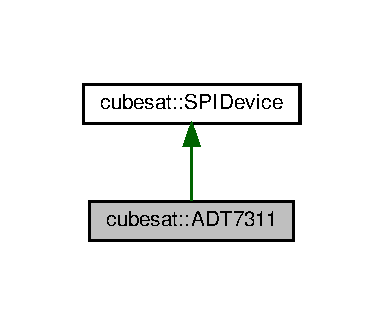
\includegraphics[width=184pt]{classcubesat_1_1ADT7311__inherit__graph}
\end{center}
\end{figure}


Collaboration diagram for cubesat\+:\+:A\+D\+T7311\+:\nopagebreak
\begin{figure}[H]
\begin{center}
\leavevmode
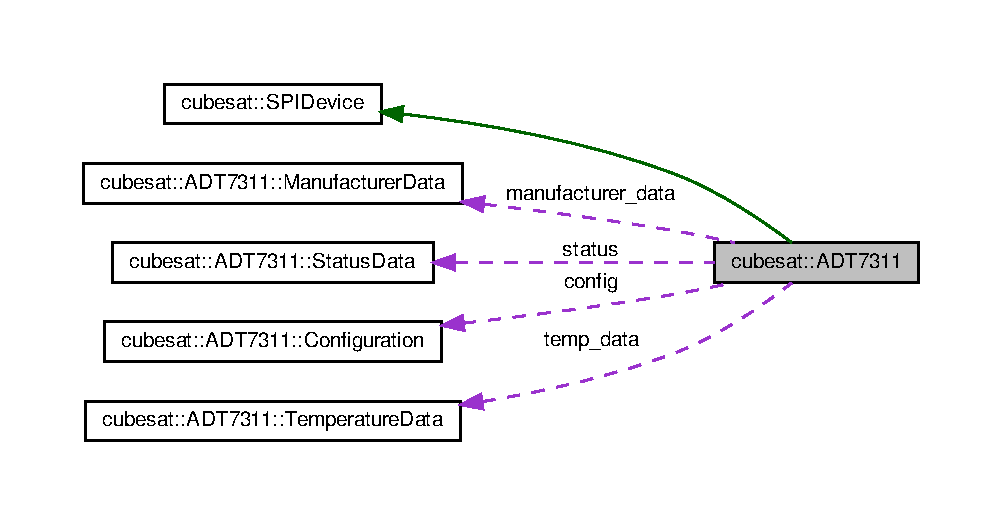
\includegraphics[width=350pt]{classcubesat_1_1ADT7311__coll__graph}
\end{center}
\end{figure}
\subsection*{Classes}
\begin{DoxyCompactItemize}
\item 
union \hyperlink{unioncubesat_1_1ADT7311_1_1Configuration}{Configuration}
\begin{DoxyCompactList}\small\item\em \hyperlink{unioncubesat_1_1ADT7311_1_1Configuration}{Configuration} flags. \end{DoxyCompactList}\item 
union \hyperlink{unioncubesat_1_1ADT7311_1_1ManufacturerData}{Manufacturer\+Data}
\begin{DoxyCompactList}\small\item\em Stores data from the Manufacturer ID register. \end{DoxyCompactList}\item 
union \hyperlink{unioncubesat_1_1ADT7311_1_1StatusData}{Status\+Data}
\begin{DoxyCompactList}\small\item\em Stores data from the Status register. \end{DoxyCompactList}\item 
union \hyperlink{unioncubesat_1_1ADT7311_1_1TemperatureData}{Temperature\+Data}
\begin{DoxyCompactList}\small\item\em Stores temperature data for 13-\/bit resolution mode. \end{DoxyCompactList}\end{DoxyCompactItemize}
\subsection*{Public Types}
\begin{DoxyCompactItemize}
\item 
enum \hyperlink{classcubesat_1_1ADT7311_a0c841a239b3da653d4304377b3e83b45}{Register} \+: uint8\+\_\+t \{ \newline
\hyperlink{classcubesat_1_1ADT7311_a0c841a239b3da653d4304377b3e83b45aec53a8c4f07baed5d8825072c89799be}{Register\+::\+Status} = 0x00, 
\hyperlink{classcubesat_1_1ADT7311_a0c841a239b3da653d4304377b3e83b45afa535ffb25e1fd20341652f9be21e06e}{Register\+::\+Config} = 0x01, 
\hyperlink{classcubesat_1_1ADT7311_a0c841a239b3da653d4304377b3e83b45aee7a8e262285ed49ea1b4e4ae11525bd}{Register\+::\+Temperature} = 0x02, 
\hyperlink{classcubesat_1_1ADT7311_a0c841a239b3da653d4304377b3e83b45aa7d89735574041405dafefe7c2c15afb}{Register\+::\+Manufacturer\+\_\+\+ID} = 0x03, 
\newline
\hyperlink{classcubesat_1_1ADT7311_a0c841a239b3da653d4304377b3e83b45ad7a94d133d1316be5d89f1cd8796b7fa}{Register\+::\+Crit\+Set\+Point} = 0x04, 
\hyperlink{classcubesat_1_1ADT7311_a0c841a239b3da653d4304377b3e83b45aa904db05d93ac11f90d0c6dabdbca25c}{Register\+::\+Hyst\+Set\+Point} = 0x05, 
\hyperlink{classcubesat_1_1ADT7311_a0c841a239b3da653d4304377b3e83b45a0c6f114f7df080df2f10b75e96223dc3}{Register\+::\+High\+Set\+Point} = 0x06, 
\hyperlink{classcubesat_1_1ADT7311_a0c841a239b3da653d4304377b3e83b45a4011b21f421577265c398f33412b0216}{Register\+::\+Low\+Set\+Point} = 0x07
 \}\begin{DoxyCompactList}\small\item\em Register addresses. \end{DoxyCompactList}
\end{DoxyCompactItemize}
\subsection*{Public Member Functions}
\begin{DoxyCompactItemize}
\item 
\hyperlink{classcubesat_1_1ADT7311_a78925b45d39fe44bd7cf1fb706a6d5c1}{A\+D\+T7311} ()
\item 
\hyperlink{classcubesat_1_1ADT7311_ae20c3e2e7668a0b93494dd1e2fb89d8d}{A\+D\+T7311} (unsigned int \hyperlink{classcubesat_1_1SPIDevice_a4b4e91bed3762e7c7e4399fba3cb386d}{bus}, unsigned int \hyperlink{classcubesat_1_1SPIDevice_aa771ccb034a870a9188e63600fd4b40a}{device})
\begin{DoxyCompactList}\small\item\em Constructs a new \hyperlink{classcubesat_1_1ADT7311}{A\+D\+T7311} object with the given bus and device address. \end{DoxyCompactList}\item 
virtual \hyperlink{classcubesat_1_1ADT7311_a2f45a357a557098fcf9d72b6087e731c}{$\sim$\+A\+D\+T7311} ()
\begin{DoxyCompactList}\small\item\em Destructor. \end{DoxyCompactList}\item 
virtual int \hyperlink{classcubesat_1_1ADT7311_ac8ddceb62b008effe3f4521bbbe154f7}{Open} () override
\item 
void \hyperlink{classcubesat_1_1ADT7311_a30816e820813a843a945583572676c13}{Read\+State} ()
\begin{DoxyCompactList}\small\item\em Reads and stores information from the device. \end{DoxyCompactList}\item 
void \hyperlink{classcubesat_1_1ADT7311_adaafd79f27e3929eeba00c0a185d5b32}{Set\+Configuration} (\hyperlink{unioncubesat_1_1ADT7311_1_1Configuration}{Configuration} \&\hyperlink{classcubesat_1_1ADT7311_aa14e2538b100b5427358cf21fff183e6}{config})
\begin{DoxyCompactList}\small\item\em Writes to the configuration register. \end{DoxyCompactList}\item 
void \hyperlink{classcubesat_1_1ADT7311_a52ef57ca7df4c0f53ed0f98be1c1defd}{Set\+Low\+Setpoint} (int16\+\_\+t temp)
\begin{DoxyCompactList}\small\item\em Writes to the low setpoint register. \end{DoxyCompactList}\item 
void \hyperlink{classcubesat_1_1ADT7311_a6e2fef4825d733d11fed423e0c19edcd}{Set\+High\+Setpoint} (int16\+\_\+t temp)
\begin{DoxyCompactList}\small\item\em Writes to the high setpoint register. \end{DoxyCompactList}\item 
void \hyperlink{classcubesat_1_1ADT7311_a769bd9152682b5ebd7408d1796116b71}{Set\+Hyst\+Setpoint} (uint8\+\_\+t temp)
\begin{DoxyCompactList}\small\item\em Writes to the hyst. setpoint register. \end{DoxyCompactList}\item 
void \hyperlink{classcubesat_1_1ADT7311_a5351ef5f5982332d1a8a08677f93e859}{Set\+Crit\+Setpoint} (int16\+\_\+t temp)
\begin{DoxyCompactList}\small\item\em Writes to the critical setpoint register. \end{DoxyCompactList}\item 
int16\+\_\+t \hyperlink{classcubesat_1_1ADT7311_a4d2ab8dec28559cd1d2a2030b2b828d2}{Get\+Low\+Setpoint} () const
\begin{DoxyCompactList}\small\item\em Retrieves the low setpoint value. \end{DoxyCompactList}\item 
int16\+\_\+t \hyperlink{classcubesat_1_1ADT7311_adb40c389c5e36aa4c2f0e59712df9333}{Get\+High\+Setpoint} () const
\begin{DoxyCompactList}\small\item\em Retrieves the high setpoint value. \end{DoxyCompactList}\item 
int16\+\_\+t \hyperlink{classcubesat_1_1ADT7311_ace49d19de024ba042aa8f9cfd6aee526}{Get\+Crit\+Setpoint} () const
\begin{DoxyCompactList}\small\item\em Retrieves the critical setpoint value. \end{DoxyCompactList}\item 
uint8\+\_\+t \hyperlink{classcubesat_1_1ADT7311_a9e7fd53a9da8c18626f766cafa2afe76}{Get\+Hyst\+Setpoint} () const
\begin{DoxyCompactList}\small\item\em Retrieves the hyst. setpoint value. \end{DoxyCompactList}\item 
float \hyperlink{classcubesat_1_1ADT7311_ae9d908dd010582e8c1fe6b56826bbcbc}{Get\+Temperature} () const
\begin{DoxyCompactList}\small\item\em Returns the latest temperature reading. \end{DoxyCompactList}\item 
bool \hyperlink{classcubesat_1_1ADT7311_aa72c15f502541eb8fbfff33b77a27423}{Get\+Low\+Temp\+Flag} () const
\begin{DoxyCompactList}\small\item\em Checks if the low temperature flag was triggered. \end{DoxyCompactList}\item 
bool \hyperlink{classcubesat_1_1ADT7311_a7c4ec1475995dd4461ad8813eeebc384}{Get\+High\+Temp\+Flag} () const
\begin{DoxyCompactList}\small\item\em Checks if the high temperature flag was triggered. \end{DoxyCompactList}\item 
bool \hyperlink{classcubesat_1_1ADT7311_ad82d5473a3f07b5cb85cc4af670bba28}{Get\+Crit\+Temp\+Flag} () const
\begin{DoxyCompactList}\small\item\em Checks if the critical temperature flag was triggered. \end{DoxyCompactList}\item 
\hyperlink{unioncubesat_1_1ADT7311_1_1Configuration}{Configuration} \hyperlink{classcubesat_1_1ADT7311_af51b8fd845ccdabb5be82263025de820}{Get\+Configuration} () const
\item 
\hyperlink{unioncubesat_1_1ADT7311_1_1TemperatureData}{Temperature\+Data} \hyperlink{classcubesat_1_1ADT7311_a84b567fb73e84dca956b9129a020f7ed}{Get\+Temperature\+Register} () const
\item 
\hyperlink{unioncubesat_1_1ADT7311_1_1StatusData}{Status\+Data} \hyperlink{classcubesat_1_1ADT7311_abb9e10d67c752e460f50c964cae84661}{Get\+Status\+Register} () const
\item 
\hyperlink{unioncubesat_1_1ADT7311_1_1ManufacturerData}{Manufacturer\+Data} \hyperlink{classcubesat_1_1ADT7311_a7bee01cf24697f23b6e6ec236fab7966}{Get\+Manufacturer\+Register} () const
\item 
uint16\+\_\+t \hyperlink{classcubesat_1_1ADT7311_a504905f3649b3013f3f2d1ffe3676376}{Get\+Crit\+Setpoint\+Register} () const
\item 
uint8\+\_\+t \hyperlink{classcubesat_1_1ADT7311_a8b2cf374d18a6bc05a8529a4e667face}{Get\+Hyst\+Setpoint\+Register} () const
\item 
uint16\+\_\+t \hyperlink{classcubesat_1_1ADT7311_a1cc3625e29758f775de262aaea89b0f1}{Get\+Low\+Setpoint\+Register} () const
\item 
uint16\+\_\+t \hyperlink{classcubesat_1_1ADT7311_a97830a383f0149caf364a5e135d75835}{Get\+High\+Setpoint\+Register} () const
\end{DoxyCompactItemize}
\subsection*{Private Types}
\begin{DoxyCompactItemize}
\item 
enum \hyperlink{classcubesat_1_1ADT7311_a4a6cb79b6b3ec095455c94b20c9ca59e}{Command\+Mode} \+: uint8\+\_\+t \{ \hyperlink{classcubesat_1_1ADT7311_a4a6cb79b6b3ec095455c94b20c9ca59ead4d157343baa33cf5c433a363aee8da3}{Write} = 0, 
\hyperlink{classcubesat_1_1ADT7311_a4a6cb79b6b3ec095455c94b20c9ca59eabcbc3270c2b985ad1692355475b67986}{Read} = 1
 \}
\end{DoxyCompactItemize}
\subsection*{Private Member Functions}
\begin{DoxyCompactItemize}
\item 
uint8\+\_\+t \hyperlink{classcubesat_1_1ADT7311_afa5e19c1e97ce0623c658120f3c02027}{Get\+Command} (\hyperlink{classcubesat_1_1ADT7311_a4a6cb79b6b3ec095455c94b20c9ca59e}{Command\+Mode} \hyperlink{classcubesat_1_1SPIDevice_ac69ac6b9e9ac9ed194384a3fa07ecbde}{mode}, \hyperlink{classcubesat_1_1ADT7311_a0c841a239b3da653d4304377b3e83b45}{Register} reg)
\item 
void \hyperlink{classcubesat_1_1ADT7311_acfb6dbbe3616e39449808880f96f610c}{Write8\+Bit} (\hyperlink{classcubesat_1_1ADT7311_a0c841a239b3da653d4304377b3e83b45}{Register} reg, uint8\+\_\+t value)
\item 
void \hyperlink{classcubesat_1_1ADT7311_a78f061f3e7a5a4f060868b53839c7af6}{Write16\+Bit} (\hyperlink{classcubesat_1_1ADT7311_a0c841a239b3da653d4304377b3e83b45}{Register} reg, uint16\+\_\+t value)
\item 
uint8\+\_\+t \hyperlink{classcubesat_1_1ADT7311_a0f0c46f2a75ebb5661e27c3340b089a4}{Read8\+Bit} (\hyperlink{classcubesat_1_1ADT7311_a0c841a239b3da653d4304377b3e83b45}{Register} reg)
\item 
uint16\+\_\+t \hyperlink{classcubesat_1_1ADT7311_a9147cb2c01b121fe0576eb36c9fcc18f}{Read16\+Bit} (\hyperlink{classcubesat_1_1ADT7311_a0c841a239b3da653d4304377b3e83b45}{Register} reg)
\end{DoxyCompactItemize}
\subsection*{Private Attributes}
\begin{DoxyCompactItemize}
\item 
\hyperlink{unioncubesat_1_1ADT7311_1_1Configuration}{Configuration} \hyperlink{classcubesat_1_1ADT7311_aa14e2538b100b5427358cf21fff183e6}{config}
\item 
\hyperlink{unioncubesat_1_1ADT7311_1_1StatusData}{Status\+Data} \hyperlink{classcubesat_1_1ADT7311_a4d64ee91316d0a3f44384f57bee01d17}{status}
\item 
\hyperlink{unioncubesat_1_1ADT7311_1_1TemperatureData}{Temperature\+Data} \hyperlink{classcubesat_1_1ADT7311_a8045af6862135c6796ea97b95e431705}{temp\+\_\+data}
\item 
\hyperlink{unioncubesat_1_1ADT7311_1_1ManufacturerData}{Manufacturer\+Data} \hyperlink{classcubesat_1_1ADT7311_adca4665892622e13f6dc7405528697d6}{manufacturer\+\_\+data}
\item 
uint16\+\_\+t \hyperlink{classcubesat_1_1ADT7311_a5239e3277f763a5d9cbdda84fc6476b1}{low\+\_\+setpoint}
\item 
uint16\+\_\+t \hyperlink{classcubesat_1_1ADT7311_a24bf458335fd8dce02f43f0d66ec323a}{high\+\_\+setpoint}
\item 
uint16\+\_\+t \hyperlink{classcubesat_1_1ADT7311_ab79d199972c7f14cab10015034cf6b52}{crit\+\_\+setpoint}
\item 
uint8\+\_\+t \hyperlink{classcubesat_1_1ADT7311_a486d810e54eae5c266a2c640725a4885}{hyst\+\_\+setpoint}
\end{DoxyCompactItemize}
\subsection*{Additional Inherited Members}


\subsection{Detailed Description}
Provides access to the \hyperlink{classcubesat_1_1ADT7311}{A\+D\+T7311} temperature sensor. 

\subsection{Member Enumeration Documentation}
\mbox{\Hypertarget{classcubesat_1_1ADT7311_a4a6cb79b6b3ec095455c94b20c9ca59e}\label{classcubesat_1_1ADT7311_a4a6cb79b6b3ec095455c94b20c9ca59e}} 
\index{cubesat\+::\+A\+D\+T7311@{cubesat\+::\+A\+D\+T7311}!Command\+Mode@{Command\+Mode}}
\index{Command\+Mode@{Command\+Mode}!cubesat\+::\+A\+D\+T7311@{cubesat\+::\+A\+D\+T7311}}
\subsubsection{\texorpdfstring{Command\+Mode}{CommandMode}}
{\footnotesize\ttfamily enum \hyperlink{classcubesat_1_1ADT7311_a4a6cb79b6b3ec095455c94b20c9ca59e}{cubesat\+::\+A\+D\+T7311\+::\+Command\+Mode} \+: uint8\+\_\+t\hspace{0.3cm}{\ttfamily [private]}}

\begin{DoxyEnumFields}{Enumerator}
\raisebox{\heightof{T}}[0pt][0pt]{\index{Write@{Write}!cubesat\+::\+A\+D\+T7311@{cubesat\+::\+A\+D\+T7311}}\index{cubesat\+::\+A\+D\+T7311@{cubesat\+::\+A\+D\+T7311}!Write@{Write}}}\mbox{\Hypertarget{classcubesat_1_1ADT7311_a4a6cb79b6b3ec095455c94b20c9ca59ead4d157343baa33cf5c433a363aee8da3}\label{classcubesat_1_1ADT7311_a4a6cb79b6b3ec095455c94b20c9ca59ead4d157343baa33cf5c433a363aee8da3}} 
Write&\\
\hline

\raisebox{\heightof{T}}[0pt][0pt]{\index{Read@{Read}!cubesat\+::\+A\+D\+T7311@{cubesat\+::\+A\+D\+T7311}}\index{cubesat\+::\+A\+D\+T7311@{cubesat\+::\+A\+D\+T7311}!Read@{Read}}}\mbox{\Hypertarget{classcubesat_1_1ADT7311_a4a6cb79b6b3ec095455c94b20c9ca59eabcbc3270c2b985ad1692355475b67986}\label{classcubesat_1_1ADT7311_a4a6cb79b6b3ec095455c94b20c9ca59eabcbc3270c2b985ad1692355475b67986}} 
Read&\\
\hline

\end{DoxyEnumFields}
\mbox{\Hypertarget{classcubesat_1_1ADT7311_a0c841a239b3da653d4304377b3e83b45}\label{classcubesat_1_1ADT7311_a0c841a239b3da653d4304377b3e83b45}} 
\index{cubesat\+::\+A\+D\+T7311@{cubesat\+::\+A\+D\+T7311}!Register@{Register}}
\index{Register@{Register}!cubesat\+::\+A\+D\+T7311@{cubesat\+::\+A\+D\+T7311}}
\subsubsection{\texorpdfstring{Register}{Register}}
{\footnotesize\ttfamily enum \hyperlink{classcubesat_1_1ADT7311_a0c841a239b3da653d4304377b3e83b45}{cubesat\+::\+A\+D\+T7311\+::\+Register} \+: uint8\+\_\+t\hspace{0.3cm}{\ttfamily [strong]}}



Register addresses. 

\begin{DoxyEnumFields}{Enumerator}
\raisebox{\heightof{T}}[0pt][0pt]{\index{Status@{Status}!cubesat\+::\+A\+D\+T7311@{cubesat\+::\+A\+D\+T7311}}\index{cubesat\+::\+A\+D\+T7311@{cubesat\+::\+A\+D\+T7311}!Status@{Status}}}\mbox{\Hypertarget{classcubesat_1_1ADT7311_a0c841a239b3da653d4304377b3e83b45aec53a8c4f07baed5d8825072c89799be}\label{classcubesat_1_1ADT7311_a0c841a239b3da653d4304377b3e83b45aec53a8c4f07baed5d8825072c89799be}} 
Status&\\
\hline

\raisebox{\heightof{T}}[0pt][0pt]{\index{Config@{Config}!cubesat\+::\+A\+D\+T7311@{cubesat\+::\+A\+D\+T7311}}\index{cubesat\+::\+A\+D\+T7311@{cubesat\+::\+A\+D\+T7311}!Config@{Config}}}\mbox{\Hypertarget{classcubesat_1_1ADT7311_a0c841a239b3da653d4304377b3e83b45afa535ffb25e1fd20341652f9be21e06e}\label{classcubesat_1_1ADT7311_a0c841a239b3da653d4304377b3e83b45afa535ffb25e1fd20341652f9be21e06e}} 
Config&\\
\hline

\raisebox{\heightof{T}}[0pt][0pt]{\index{Temperature@{Temperature}!cubesat\+::\+A\+D\+T7311@{cubesat\+::\+A\+D\+T7311}}\index{cubesat\+::\+A\+D\+T7311@{cubesat\+::\+A\+D\+T7311}!Temperature@{Temperature}}}\mbox{\Hypertarget{classcubesat_1_1ADT7311_a0c841a239b3da653d4304377b3e83b45aee7a8e262285ed49ea1b4e4ae11525bd}\label{classcubesat_1_1ADT7311_a0c841a239b3da653d4304377b3e83b45aee7a8e262285ed49ea1b4e4ae11525bd}} 
Temperature&\\
\hline

\raisebox{\heightof{T}}[0pt][0pt]{\index{Manufacturer\+\_\+\+ID@{Manufacturer\+\_\+\+ID}!cubesat\+::\+A\+D\+T7311@{cubesat\+::\+A\+D\+T7311}}\index{cubesat\+::\+A\+D\+T7311@{cubesat\+::\+A\+D\+T7311}!Manufacturer\+\_\+\+ID@{Manufacturer\+\_\+\+ID}}}\mbox{\Hypertarget{classcubesat_1_1ADT7311_a0c841a239b3da653d4304377b3e83b45aa7d89735574041405dafefe7c2c15afb}\label{classcubesat_1_1ADT7311_a0c841a239b3da653d4304377b3e83b45aa7d89735574041405dafefe7c2c15afb}} 
Manufacturer\+\_\+\+ID&\\
\hline

\raisebox{\heightof{T}}[0pt][0pt]{\index{Crit\+Set\+Point@{Crit\+Set\+Point}!cubesat\+::\+A\+D\+T7311@{cubesat\+::\+A\+D\+T7311}}\index{cubesat\+::\+A\+D\+T7311@{cubesat\+::\+A\+D\+T7311}!Crit\+Set\+Point@{Crit\+Set\+Point}}}\mbox{\Hypertarget{classcubesat_1_1ADT7311_a0c841a239b3da653d4304377b3e83b45ad7a94d133d1316be5d89f1cd8796b7fa}\label{classcubesat_1_1ADT7311_a0c841a239b3da653d4304377b3e83b45ad7a94d133d1316be5d89f1cd8796b7fa}} 
Crit\+Set\+Point&\\
\hline

\raisebox{\heightof{T}}[0pt][0pt]{\index{Hyst\+Set\+Point@{Hyst\+Set\+Point}!cubesat\+::\+A\+D\+T7311@{cubesat\+::\+A\+D\+T7311}}\index{cubesat\+::\+A\+D\+T7311@{cubesat\+::\+A\+D\+T7311}!Hyst\+Set\+Point@{Hyst\+Set\+Point}}}\mbox{\Hypertarget{classcubesat_1_1ADT7311_a0c841a239b3da653d4304377b3e83b45aa904db05d93ac11f90d0c6dabdbca25c}\label{classcubesat_1_1ADT7311_a0c841a239b3da653d4304377b3e83b45aa904db05d93ac11f90d0c6dabdbca25c}} 
Hyst\+Set\+Point&\\
\hline

\raisebox{\heightof{T}}[0pt][0pt]{\index{High\+Set\+Point@{High\+Set\+Point}!cubesat\+::\+A\+D\+T7311@{cubesat\+::\+A\+D\+T7311}}\index{cubesat\+::\+A\+D\+T7311@{cubesat\+::\+A\+D\+T7311}!High\+Set\+Point@{High\+Set\+Point}}}\mbox{\Hypertarget{classcubesat_1_1ADT7311_a0c841a239b3da653d4304377b3e83b45a0c6f114f7df080df2f10b75e96223dc3}\label{classcubesat_1_1ADT7311_a0c841a239b3da653d4304377b3e83b45a0c6f114f7df080df2f10b75e96223dc3}} 
High\+Set\+Point&\\
\hline

\raisebox{\heightof{T}}[0pt][0pt]{\index{Low\+Set\+Point@{Low\+Set\+Point}!cubesat\+::\+A\+D\+T7311@{cubesat\+::\+A\+D\+T7311}}\index{cubesat\+::\+A\+D\+T7311@{cubesat\+::\+A\+D\+T7311}!Low\+Set\+Point@{Low\+Set\+Point}}}\mbox{\Hypertarget{classcubesat_1_1ADT7311_a0c841a239b3da653d4304377b3e83b45a4011b21f421577265c398f33412b0216}\label{classcubesat_1_1ADT7311_a0c841a239b3da653d4304377b3e83b45a4011b21f421577265c398f33412b0216}} 
Low\+Set\+Point&\\
\hline

\end{DoxyEnumFields}


\subsection{Constructor \& Destructor Documentation}
\mbox{\Hypertarget{classcubesat_1_1ADT7311_a78925b45d39fe44bd7cf1fb706a6d5c1}\label{classcubesat_1_1ADT7311_a78925b45d39fe44bd7cf1fb706a6d5c1}} 
\index{cubesat\+::\+A\+D\+T7311@{cubesat\+::\+A\+D\+T7311}!A\+D\+T7311@{A\+D\+T7311}}
\index{A\+D\+T7311@{A\+D\+T7311}!cubesat\+::\+A\+D\+T7311@{cubesat\+::\+A\+D\+T7311}}
\subsubsection{\texorpdfstring{A\+D\+T7311()}{ADT7311()}\hspace{0.1cm}{\footnotesize\ttfamily [1/2]}}
{\footnotesize\ttfamily cubesat\+::\+A\+D\+T7311\+::\+A\+D\+T7311 (\begin{DoxyParamCaption}{ }\end{DoxyParamCaption})\hspace{0.3cm}{\ttfamily [inline]}}

\mbox{\Hypertarget{classcubesat_1_1ADT7311_ae20c3e2e7668a0b93494dd1e2fb89d8d}\label{classcubesat_1_1ADT7311_ae20c3e2e7668a0b93494dd1e2fb89d8d}} 
\index{cubesat\+::\+A\+D\+T7311@{cubesat\+::\+A\+D\+T7311}!A\+D\+T7311@{A\+D\+T7311}}
\index{A\+D\+T7311@{A\+D\+T7311}!cubesat\+::\+A\+D\+T7311@{cubesat\+::\+A\+D\+T7311}}
\subsubsection{\texorpdfstring{A\+D\+T7311()}{ADT7311()}\hspace{0.1cm}{\footnotesize\ttfamily [2/2]}}
{\footnotesize\ttfamily A\+D\+T7311\+::\+A\+D\+T7311 (\begin{DoxyParamCaption}\item[{unsigned int}]{bus,  }\item[{unsigned int}]{device }\end{DoxyParamCaption})}



Constructs a new \hyperlink{classcubesat_1_1ADT7311}{A\+D\+T7311} object with the given bus and device address. 


\begin{DoxyParams}{Parameters}
{\em bus} & The bus address \\
\hline
{\em device} & The device address \\
\hline
\end{DoxyParams}
\mbox{\Hypertarget{classcubesat_1_1ADT7311_a2f45a357a557098fcf9d72b6087e731c}\label{classcubesat_1_1ADT7311_a2f45a357a557098fcf9d72b6087e731c}} 
\index{cubesat\+::\+A\+D\+T7311@{cubesat\+::\+A\+D\+T7311}!````~A\+D\+T7311@{$\sim$\+A\+D\+T7311}}
\index{````~A\+D\+T7311@{$\sim$\+A\+D\+T7311}!cubesat\+::\+A\+D\+T7311@{cubesat\+::\+A\+D\+T7311}}
\subsubsection{\texorpdfstring{$\sim$\+A\+D\+T7311()}{~ADT7311()}}
{\footnotesize\ttfamily A\+D\+T7311\+::$\sim$\+A\+D\+T7311 (\begin{DoxyParamCaption}{ }\end{DoxyParamCaption})\hspace{0.3cm}{\ttfamily [virtual]}}



Destructor. 



\subsection{Member Function Documentation}
\mbox{\Hypertarget{classcubesat_1_1ADT7311_afa5e19c1e97ce0623c658120f3c02027}\label{classcubesat_1_1ADT7311_afa5e19c1e97ce0623c658120f3c02027}} 
\index{cubesat\+::\+A\+D\+T7311@{cubesat\+::\+A\+D\+T7311}!Get\+Command@{Get\+Command}}
\index{Get\+Command@{Get\+Command}!cubesat\+::\+A\+D\+T7311@{cubesat\+::\+A\+D\+T7311}}
\subsubsection{\texorpdfstring{Get\+Command()}{GetCommand()}}
{\footnotesize\ttfamily uint8\+\_\+t A\+D\+T7311\+::\+Get\+Command (\begin{DoxyParamCaption}\item[{\hyperlink{classcubesat_1_1ADT7311_a4a6cb79b6b3ec095455c94b20c9ca59e}{Command\+Mode}}]{mode,  }\item[{\hyperlink{classcubesat_1_1ADT7311_a0c841a239b3da653d4304377b3e83b45}{Register}}]{reg }\end{DoxyParamCaption})\hspace{0.3cm}{\ttfamily [private]}}

\mbox{\Hypertarget{classcubesat_1_1ADT7311_af51b8fd845ccdabb5be82263025de820}\label{classcubesat_1_1ADT7311_af51b8fd845ccdabb5be82263025de820}} 
\index{cubesat\+::\+A\+D\+T7311@{cubesat\+::\+A\+D\+T7311}!Get\+Configuration@{Get\+Configuration}}
\index{Get\+Configuration@{Get\+Configuration}!cubesat\+::\+A\+D\+T7311@{cubesat\+::\+A\+D\+T7311}}
\subsubsection{\texorpdfstring{Get\+Configuration()}{GetConfiguration()}}
{\footnotesize\ttfamily \hyperlink{unioncubesat_1_1ADT7311_1_1Configuration}{Configuration} cubesat\+::\+A\+D\+T7311\+::\+Get\+Configuration (\begin{DoxyParamCaption}{ }\end{DoxyParamCaption}) const\hspace{0.3cm}{\ttfamily [inline]}}

\mbox{\Hypertarget{classcubesat_1_1ADT7311_ace49d19de024ba042aa8f9cfd6aee526}\label{classcubesat_1_1ADT7311_ace49d19de024ba042aa8f9cfd6aee526}} 
\index{cubesat\+::\+A\+D\+T7311@{cubesat\+::\+A\+D\+T7311}!Get\+Crit\+Setpoint@{Get\+Crit\+Setpoint}}
\index{Get\+Crit\+Setpoint@{Get\+Crit\+Setpoint}!cubesat\+::\+A\+D\+T7311@{cubesat\+::\+A\+D\+T7311}}
\subsubsection{\texorpdfstring{Get\+Crit\+Setpoint()}{GetCritSetpoint()}}
{\footnotesize\ttfamily int16\+\_\+t cubesat\+::\+A\+D\+T7311\+::\+Get\+Crit\+Setpoint (\begin{DoxyParamCaption}{ }\end{DoxyParamCaption}) const\hspace{0.3cm}{\ttfamily [inline]}}



Retrieves the critical setpoint value. 

\begin{DoxyReturn}{Returns}
The critical setpoint in celcius 
\end{DoxyReturn}
\mbox{\Hypertarget{classcubesat_1_1ADT7311_a504905f3649b3013f3f2d1ffe3676376}\label{classcubesat_1_1ADT7311_a504905f3649b3013f3f2d1ffe3676376}} 
\index{cubesat\+::\+A\+D\+T7311@{cubesat\+::\+A\+D\+T7311}!Get\+Crit\+Setpoint\+Register@{Get\+Crit\+Setpoint\+Register}}
\index{Get\+Crit\+Setpoint\+Register@{Get\+Crit\+Setpoint\+Register}!cubesat\+::\+A\+D\+T7311@{cubesat\+::\+A\+D\+T7311}}
\subsubsection{\texorpdfstring{Get\+Crit\+Setpoint\+Register()}{GetCritSetpointRegister()}}
{\footnotesize\ttfamily uint16\+\_\+t cubesat\+::\+A\+D\+T7311\+::\+Get\+Crit\+Setpoint\+Register (\begin{DoxyParamCaption}{ }\end{DoxyParamCaption}) const\hspace{0.3cm}{\ttfamily [inline]}}

\mbox{\Hypertarget{classcubesat_1_1ADT7311_ad82d5473a3f07b5cb85cc4af670bba28}\label{classcubesat_1_1ADT7311_ad82d5473a3f07b5cb85cc4af670bba28}} 
\index{cubesat\+::\+A\+D\+T7311@{cubesat\+::\+A\+D\+T7311}!Get\+Crit\+Temp\+Flag@{Get\+Crit\+Temp\+Flag}}
\index{Get\+Crit\+Temp\+Flag@{Get\+Crit\+Temp\+Flag}!cubesat\+::\+A\+D\+T7311@{cubesat\+::\+A\+D\+T7311}}
\subsubsection{\texorpdfstring{Get\+Crit\+Temp\+Flag()}{GetCritTempFlag()}}
{\footnotesize\ttfamily bool cubesat\+::\+A\+D\+T7311\+::\+Get\+Crit\+Temp\+Flag (\begin{DoxyParamCaption}{ }\end{DoxyParamCaption}) const\hspace{0.3cm}{\ttfamily [inline]}}



Checks if the critical temperature flag was triggered. 

\begin{DoxyReturn}{Returns}
True if set, false if not 
\end{DoxyReturn}
\mbox{\Hypertarget{classcubesat_1_1ADT7311_adb40c389c5e36aa4c2f0e59712df9333}\label{classcubesat_1_1ADT7311_adb40c389c5e36aa4c2f0e59712df9333}} 
\index{cubesat\+::\+A\+D\+T7311@{cubesat\+::\+A\+D\+T7311}!Get\+High\+Setpoint@{Get\+High\+Setpoint}}
\index{Get\+High\+Setpoint@{Get\+High\+Setpoint}!cubesat\+::\+A\+D\+T7311@{cubesat\+::\+A\+D\+T7311}}
\subsubsection{\texorpdfstring{Get\+High\+Setpoint()}{GetHighSetpoint()}}
{\footnotesize\ttfamily int16\+\_\+t cubesat\+::\+A\+D\+T7311\+::\+Get\+High\+Setpoint (\begin{DoxyParamCaption}{ }\end{DoxyParamCaption}) const\hspace{0.3cm}{\ttfamily [inline]}}



Retrieves the high setpoint value. 

\begin{DoxyReturn}{Returns}
The high setpoint in celcius 
\end{DoxyReturn}
\mbox{\Hypertarget{classcubesat_1_1ADT7311_a97830a383f0149caf364a5e135d75835}\label{classcubesat_1_1ADT7311_a97830a383f0149caf364a5e135d75835}} 
\index{cubesat\+::\+A\+D\+T7311@{cubesat\+::\+A\+D\+T7311}!Get\+High\+Setpoint\+Register@{Get\+High\+Setpoint\+Register}}
\index{Get\+High\+Setpoint\+Register@{Get\+High\+Setpoint\+Register}!cubesat\+::\+A\+D\+T7311@{cubesat\+::\+A\+D\+T7311}}
\subsubsection{\texorpdfstring{Get\+High\+Setpoint\+Register()}{GetHighSetpointRegister()}}
{\footnotesize\ttfamily uint16\+\_\+t cubesat\+::\+A\+D\+T7311\+::\+Get\+High\+Setpoint\+Register (\begin{DoxyParamCaption}{ }\end{DoxyParamCaption}) const\hspace{0.3cm}{\ttfamily [inline]}}

\mbox{\Hypertarget{classcubesat_1_1ADT7311_a7c4ec1475995dd4461ad8813eeebc384}\label{classcubesat_1_1ADT7311_a7c4ec1475995dd4461ad8813eeebc384}} 
\index{cubesat\+::\+A\+D\+T7311@{cubesat\+::\+A\+D\+T7311}!Get\+High\+Temp\+Flag@{Get\+High\+Temp\+Flag}}
\index{Get\+High\+Temp\+Flag@{Get\+High\+Temp\+Flag}!cubesat\+::\+A\+D\+T7311@{cubesat\+::\+A\+D\+T7311}}
\subsubsection{\texorpdfstring{Get\+High\+Temp\+Flag()}{GetHighTempFlag()}}
{\footnotesize\ttfamily bool cubesat\+::\+A\+D\+T7311\+::\+Get\+High\+Temp\+Flag (\begin{DoxyParamCaption}{ }\end{DoxyParamCaption}) const\hspace{0.3cm}{\ttfamily [inline]}}



Checks if the high temperature flag was triggered. 

\begin{DoxyReturn}{Returns}
True if set, false if not 
\end{DoxyReturn}
\mbox{\Hypertarget{classcubesat_1_1ADT7311_a9e7fd53a9da8c18626f766cafa2afe76}\label{classcubesat_1_1ADT7311_a9e7fd53a9da8c18626f766cafa2afe76}} 
\index{cubesat\+::\+A\+D\+T7311@{cubesat\+::\+A\+D\+T7311}!Get\+Hyst\+Setpoint@{Get\+Hyst\+Setpoint}}
\index{Get\+Hyst\+Setpoint@{Get\+Hyst\+Setpoint}!cubesat\+::\+A\+D\+T7311@{cubesat\+::\+A\+D\+T7311}}
\subsubsection{\texorpdfstring{Get\+Hyst\+Setpoint()}{GetHystSetpoint()}}
{\footnotesize\ttfamily uint8\+\_\+t cubesat\+::\+A\+D\+T7311\+::\+Get\+Hyst\+Setpoint (\begin{DoxyParamCaption}{ }\end{DoxyParamCaption}) const\hspace{0.3cm}{\ttfamily [inline]}}



Retrieves the hyst. setpoint value. 

\begin{DoxyReturn}{Returns}
The hyst. setpoint in celcius 
\end{DoxyReturn}
\mbox{\Hypertarget{classcubesat_1_1ADT7311_a8b2cf374d18a6bc05a8529a4e667face}\label{classcubesat_1_1ADT7311_a8b2cf374d18a6bc05a8529a4e667face}} 
\index{cubesat\+::\+A\+D\+T7311@{cubesat\+::\+A\+D\+T7311}!Get\+Hyst\+Setpoint\+Register@{Get\+Hyst\+Setpoint\+Register}}
\index{Get\+Hyst\+Setpoint\+Register@{Get\+Hyst\+Setpoint\+Register}!cubesat\+::\+A\+D\+T7311@{cubesat\+::\+A\+D\+T7311}}
\subsubsection{\texorpdfstring{Get\+Hyst\+Setpoint\+Register()}{GetHystSetpointRegister()}}
{\footnotesize\ttfamily uint8\+\_\+t cubesat\+::\+A\+D\+T7311\+::\+Get\+Hyst\+Setpoint\+Register (\begin{DoxyParamCaption}{ }\end{DoxyParamCaption}) const\hspace{0.3cm}{\ttfamily [inline]}}

\mbox{\Hypertarget{classcubesat_1_1ADT7311_a4d2ab8dec28559cd1d2a2030b2b828d2}\label{classcubesat_1_1ADT7311_a4d2ab8dec28559cd1d2a2030b2b828d2}} 
\index{cubesat\+::\+A\+D\+T7311@{cubesat\+::\+A\+D\+T7311}!Get\+Low\+Setpoint@{Get\+Low\+Setpoint}}
\index{Get\+Low\+Setpoint@{Get\+Low\+Setpoint}!cubesat\+::\+A\+D\+T7311@{cubesat\+::\+A\+D\+T7311}}
\subsubsection{\texorpdfstring{Get\+Low\+Setpoint()}{GetLowSetpoint()}}
{\footnotesize\ttfamily int16\+\_\+t cubesat\+::\+A\+D\+T7311\+::\+Get\+Low\+Setpoint (\begin{DoxyParamCaption}{ }\end{DoxyParamCaption}) const\hspace{0.3cm}{\ttfamily [inline]}}



Retrieves the low setpoint value. 

\begin{DoxyReturn}{Returns}
The low setpoint in celcius 
\end{DoxyReturn}
\mbox{\Hypertarget{classcubesat_1_1ADT7311_a1cc3625e29758f775de262aaea89b0f1}\label{classcubesat_1_1ADT7311_a1cc3625e29758f775de262aaea89b0f1}} 
\index{cubesat\+::\+A\+D\+T7311@{cubesat\+::\+A\+D\+T7311}!Get\+Low\+Setpoint\+Register@{Get\+Low\+Setpoint\+Register}}
\index{Get\+Low\+Setpoint\+Register@{Get\+Low\+Setpoint\+Register}!cubesat\+::\+A\+D\+T7311@{cubesat\+::\+A\+D\+T7311}}
\subsubsection{\texorpdfstring{Get\+Low\+Setpoint\+Register()}{GetLowSetpointRegister()}}
{\footnotesize\ttfamily uint16\+\_\+t cubesat\+::\+A\+D\+T7311\+::\+Get\+Low\+Setpoint\+Register (\begin{DoxyParamCaption}{ }\end{DoxyParamCaption}) const\hspace{0.3cm}{\ttfamily [inline]}}

\mbox{\Hypertarget{classcubesat_1_1ADT7311_aa72c15f502541eb8fbfff33b77a27423}\label{classcubesat_1_1ADT7311_aa72c15f502541eb8fbfff33b77a27423}} 
\index{cubesat\+::\+A\+D\+T7311@{cubesat\+::\+A\+D\+T7311}!Get\+Low\+Temp\+Flag@{Get\+Low\+Temp\+Flag}}
\index{Get\+Low\+Temp\+Flag@{Get\+Low\+Temp\+Flag}!cubesat\+::\+A\+D\+T7311@{cubesat\+::\+A\+D\+T7311}}
\subsubsection{\texorpdfstring{Get\+Low\+Temp\+Flag()}{GetLowTempFlag()}}
{\footnotesize\ttfamily bool cubesat\+::\+A\+D\+T7311\+::\+Get\+Low\+Temp\+Flag (\begin{DoxyParamCaption}{ }\end{DoxyParamCaption}) const\hspace{0.3cm}{\ttfamily [inline]}}



Checks if the low temperature flag was triggered. 

\begin{DoxyReturn}{Returns}
True if set, false if not 
\end{DoxyReturn}
\mbox{\Hypertarget{classcubesat_1_1ADT7311_a7bee01cf24697f23b6e6ec236fab7966}\label{classcubesat_1_1ADT7311_a7bee01cf24697f23b6e6ec236fab7966}} 
\index{cubesat\+::\+A\+D\+T7311@{cubesat\+::\+A\+D\+T7311}!Get\+Manufacturer\+Register@{Get\+Manufacturer\+Register}}
\index{Get\+Manufacturer\+Register@{Get\+Manufacturer\+Register}!cubesat\+::\+A\+D\+T7311@{cubesat\+::\+A\+D\+T7311}}
\subsubsection{\texorpdfstring{Get\+Manufacturer\+Register()}{GetManufacturerRegister()}}
{\footnotesize\ttfamily \hyperlink{unioncubesat_1_1ADT7311_1_1ManufacturerData}{Manufacturer\+Data} cubesat\+::\+A\+D\+T7311\+::\+Get\+Manufacturer\+Register (\begin{DoxyParamCaption}{ }\end{DoxyParamCaption}) const\hspace{0.3cm}{\ttfamily [inline]}}

\mbox{\Hypertarget{classcubesat_1_1ADT7311_abb9e10d67c752e460f50c964cae84661}\label{classcubesat_1_1ADT7311_abb9e10d67c752e460f50c964cae84661}} 
\index{cubesat\+::\+A\+D\+T7311@{cubesat\+::\+A\+D\+T7311}!Get\+Status\+Register@{Get\+Status\+Register}}
\index{Get\+Status\+Register@{Get\+Status\+Register}!cubesat\+::\+A\+D\+T7311@{cubesat\+::\+A\+D\+T7311}}
\subsubsection{\texorpdfstring{Get\+Status\+Register()}{GetStatusRegister()}}
{\footnotesize\ttfamily \hyperlink{unioncubesat_1_1ADT7311_1_1StatusData}{Status\+Data} cubesat\+::\+A\+D\+T7311\+::\+Get\+Status\+Register (\begin{DoxyParamCaption}{ }\end{DoxyParamCaption}) const\hspace{0.3cm}{\ttfamily [inline]}}

\mbox{\Hypertarget{classcubesat_1_1ADT7311_ae9d908dd010582e8c1fe6b56826bbcbc}\label{classcubesat_1_1ADT7311_ae9d908dd010582e8c1fe6b56826bbcbc}} 
\index{cubesat\+::\+A\+D\+T7311@{cubesat\+::\+A\+D\+T7311}!Get\+Temperature@{Get\+Temperature}}
\index{Get\+Temperature@{Get\+Temperature}!cubesat\+::\+A\+D\+T7311@{cubesat\+::\+A\+D\+T7311}}
\subsubsection{\texorpdfstring{Get\+Temperature()}{GetTemperature()}}
{\footnotesize\ttfamily float A\+D\+T7311\+::\+Get\+Temperature (\begin{DoxyParamCaption}{ }\end{DoxyParamCaption}) const}



Returns the latest temperature reading. 

\begin{DoxyReturn}{Returns}
The temperature in celcius 
\end{DoxyReturn}
\mbox{\Hypertarget{classcubesat_1_1ADT7311_a84b567fb73e84dca956b9129a020f7ed}\label{classcubesat_1_1ADT7311_a84b567fb73e84dca956b9129a020f7ed}} 
\index{cubesat\+::\+A\+D\+T7311@{cubesat\+::\+A\+D\+T7311}!Get\+Temperature\+Register@{Get\+Temperature\+Register}}
\index{Get\+Temperature\+Register@{Get\+Temperature\+Register}!cubesat\+::\+A\+D\+T7311@{cubesat\+::\+A\+D\+T7311}}
\subsubsection{\texorpdfstring{Get\+Temperature\+Register()}{GetTemperatureRegister()}}
{\footnotesize\ttfamily \hyperlink{unioncubesat_1_1ADT7311_1_1TemperatureData}{Temperature\+Data} cubesat\+::\+A\+D\+T7311\+::\+Get\+Temperature\+Register (\begin{DoxyParamCaption}{ }\end{DoxyParamCaption}) const\hspace{0.3cm}{\ttfamily [inline]}}

\mbox{\Hypertarget{classcubesat_1_1ADT7311_ac8ddceb62b008effe3f4521bbbe154f7}\label{classcubesat_1_1ADT7311_ac8ddceb62b008effe3f4521bbbe154f7}} 
\index{cubesat\+::\+A\+D\+T7311@{cubesat\+::\+A\+D\+T7311}!Open@{Open}}
\index{Open@{Open}!cubesat\+::\+A\+D\+T7311@{cubesat\+::\+A\+D\+T7311}}
\subsubsection{\texorpdfstring{Open()}{Open()}}
{\footnotesize\ttfamily int A\+D\+T7311\+::\+Open (\begin{DoxyParamCaption}{ }\end{DoxyParamCaption})\hspace{0.3cm}{\ttfamily [override]}, {\ttfamily [virtual]}}

This method opens the file connection to the S\+PI device. \begin{DoxyReturn}{Returns}
0 on a successful open of the file 
\end{DoxyReturn}


Reimplemented from \hyperlink{classcubesat_1_1SPIDevice_a2467a2271529579bdeaf0ffb6078b253}{cubesat\+::\+S\+P\+I\+Device}.

\mbox{\Hypertarget{classcubesat_1_1ADT7311_a9147cb2c01b121fe0576eb36c9fcc18f}\label{classcubesat_1_1ADT7311_a9147cb2c01b121fe0576eb36c9fcc18f}} 
\index{cubesat\+::\+A\+D\+T7311@{cubesat\+::\+A\+D\+T7311}!Read16\+Bit@{Read16\+Bit}}
\index{Read16\+Bit@{Read16\+Bit}!cubesat\+::\+A\+D\+T7311@{cubesat\+::\+A\+D\+T7311}}
\subsubsection{\texorpdfstring{Read16\+Bit()}{Read16Bit()}}
{\footnotesize\ttfamily uint16\+\_\+t A\+D\+T7311\+::\+Read16\+Bit (\begin{DoxyParamCaption}\item[{\hyperlink{classcubesat_1_1ADT7311_a0c841a239b3da653d4304377b3e83b45}{Register}}]{reg }\end{DoxyParamCaption})\hspace{0.3cm}{\ttfamily [private]}}

\mbox{\Hypertarget{classcubesat_1_1ADT7311_a0f0c46f2a75ebb5661e27c3340b089a4}\label{classcubesat_1_1ADT7311_a0f0c46f2a75ebb5661e27c3340b089a4}} 
\index{cubesat\+::\+A\+D\+T7311@{cubesat\+::\+A\+D\+T7311}!Read8\+Bit@{Read8\+Bit}}
\index{Read8\+Bit@{Read8\+Bit}!cubesat\+::\+A\+D\+T7311@{cubesat\+::\+A\+D\+T7311}}
\subsubsection{\texorpdfstring{Read8\+Bit()}{Read8Bit()}}
{\footnotesize\ttfamily uint8\+\_\+t A\+D\+T7311\+::\+Read8\+Bit (\begin{DoxyParamCaption}\item[{\hyperlink{classcubesat_1_1ADT7311_a0c841a239b3da653d4304377b3e83b45}{Register}}]{reg }\end{DoxyParamCaption})\hspace{0.3cm}{\ttfamily [private]}}

\mbox{\Hypertarget{classcubesat_1_1ADT7311_a30816e820813a843a945583572676c13}\label{classcubesat_1_1ADT7311_a30816e820813a843a945583572676c13}} 
\index{cubesat\+::\+A\+D\+T7311@{cubesat\+::\+A\+D\+T7311}!Read\+State@{Read\+State}}
\index{Read\+State@{Read\+State}!cubesat\+::\+A\+D\+T7311@{cubesat\+::\+A\+D\+T7311}}
\subsubsection{\texorpdfstring{Read\+State()}{ReadState()}}
{\footnotesize\ttfamily void A\+D\+T7311\+::\+Read\+State (\begin{DoxyParamCaption}{ }\end{DoxyParamCaption})}



Reads and stores information from the device. 

\mbox{\Hypertarget{classcubesat_1_1ADT7311_adaafd79f27e3929eeba00c0a185d5b32}\label{classcubesat_1_1ADT7311_adaafd79f27e3929eeba00c0a185d5b32}} 
\index{cubesat\+::\+A\+D\+T7311@{cubesat\+::\+A\+D\+T7311}!Set\+Configuration@{Set\+Configuration}}
\index{Set\+Configuration@{Set\+Configuration}!cubesat\+::\+A\+D\+T7311@{cubesat\+::\+A\+D\+T7311}}
\subsubsection{\texorpdfstring{Set\+Configuration()}{SetConfiguration()}}
{\footnotesize\ttfamily void A\+D\+T7311\+::\+Set\+Configuration (\begin{DoxyParamCaption}\item[{\hyperlink{unioncubesat_1_1ADT7311_1_1Configuration}{Configuration} \&}]{config }\end{DoxyParamCaption})}



Writes to the configuration register. 


\begin{DoxyParams}{Parameters}
{\em config} & The configuration data. \\
\hline
\end{DoxyParams}
\mbox{\Hypertarget{classcubesat_1_1ADT7311_a5351ef5f5982332d1a8a08677f93e859}\label{classcubesat_1_1ADT7311_a5351ef5f5982332d1a8a08677f93e859}} 
\index{cubesat\+::\+A\+D\+T7311@{cubesat\+::\+A\+D\+T7311}!Set\+Crit\+Setpoint@{Set\+Crit\+Setpoint}}
\index{Set\+Crit\+Setpoint@{Set\+Crit\+Setpoint}!cubesat\+::\+A\+D\+T7311@{cubesat\+::\+A\+D\+T7311}}
\subsubsection{\texorpdfstring{Set\+Crit\+Setpoint()}{SetCritSetpoint()}}
{\footnotesize\ttfamily void A\+D\+T7311\+::\+Set\+Crit\+Setpoint (\begin{DoxyParamCaption}\item[{int16\+\_\+t}]{temp }\end{DoxyParamCaption})}



Writes to the critical setpoint register. 


\begin{DoxyParams}{Parameters}
{\em temp} & The critical temperature in celcius \\
\hline
\end{DoxyParams}
\mbox{\Hypertarget{classcubesat_1_1ADT7311_a6e2fef4825d733d11fed423e0c19edcd}\label{classcubesat_1_1ADT7311_a6e2fef4825d733d11fed423e0c19edcd}} 
\index{cubesat\+::\+A\+D\+T7311@{cubesat\+::\+A\+D\+T7311}!Set\+High\+Setpoint@{Set\+High\+Setpoint}}
\index{Set\+High\+Setpoint@{Set\+High\+Setpoint}!cubesat\+::\+A\+D\+T7311@{cubesat\+::\+A\+D\+T7311}}
\subsubsection{\texorpdfstring{Set\+High\+Setpoint()}{SetHighSetpoint()}}
{\footnotesize\ttfamily void A\+D\+T7311\+::\+Set\+High\+Setpoint (\begin{DoxyParamCaption}\item[{int16\+\_\+t}]{temp }\end{DoxyParamCaption})}



Writes to the high setpoint register. 


\begin{DoxyParams}{Parameters}
{\em temp} & The high setpoint temperature in celcius \\
\hline
\end{DoxyParams}
\mbox{\Hypertarget{classcubesat_1_1ADT7311_a769bd9152682b5ebd7408d1796116b71}\label{classcubesat_1_1ADT7311_a769bd9152682b5ebd7408d1796116b71}} 
\index{cubesat\+::\+A\+D\+T7311@{cubesat\+::\+A\+D\+T7311}!Set\+Hyst\+Setpoint@{Set\+Hyst\+Setpoint}}
\index{Set\+Hyst\+Setpoint@{Set\+Hyst\+Setpoint}!cubesat\+::\+A\+D\+T7311@{cubesat\+::\+A\+D\+T7311}}
\subsubsection{\texorpdfstring{Set\+Hyst\+Setpoint()}{SetHystSetpoint()}}
{\footnotesize\ttfamily void A\+D\+T7311\+::\+Set\+Hyst\+Setpoint (\begin{DoxyParamCaption}\item[{uint8\+\_\+t}]{temp }\end{DoxyParamCaption})}



Writes to the hyst. setpoint register. 


\begin{DoxyParams}{Parameters}
{\em temp} & The hyst. temperature in celcius \\
\hline
\end{DoxyParams}
\mbox{\Hypertarget{classcubesat_1_1ADT7311_a52ef57ca7df4c0f53ed0f98be1c1defd}\label{classcubesat_1_1ADT7311_a52ef57ca7df4c0f53ed0f98be1c1defd}} 
\index{cubesat\+::\+A\+D\+T7311@{cubesat\+::\+A\+D\+T7311}!Set\+Low\+Setpoint@{Set\+Low\+Setpoint}}
\index{Set\+Low\+Setpoint@{Set\+Low\+Setpoint}!cubesat\+::\+A\+D\+T7311@{cubesat\+::\+A\+D\+T7311}}
\subsubsection{\texorpdfstring{Set\+Low\+Setpoint()}{SetLowSetpoint()}}
{\footnotesize\ttfamily void A\+D\+T7311\+::\+Set\+Low\+Setpoint (\begin{DoxyParamCaption}\item[{int16\+\_\+t}]{temp }\end{DoxyParamCaption})}



Writes to the low setpoint register. 


\begin{DoxyParams}{Parameters}
{\em temp} & The low setpoint temperature in celcius \\
\hline
\end{DoxyParams}
\mbox{\Hypertarget{classcubesat_1_1ADT7311_a78f061f3e7a5a4f060868b53839c7af6}\label{classcubesat_1_1ADT7311_a78f061f3e7a5a4f060868b53839c7af6}} 
\index{cubesat\+::\+A\+D\+T7311@{cubesat\+::\+A\+D\+T7311}!Write16\+Bit@{Write16\+Bit}}
\index{Write16\+Bit@{Write16\+Bit}!cubesat\+::\+A\+D\+T7311@{cubesat\+::\+A\+D\+T7311}}
\subsubsection{\texorpdfstring{Write16\+Bit()}{Write16Bit()}}
{\footnotesize\ttfamily void A\+D\+T7311\+::\+Write16\+Bit (\begin{DoxyParamCaption}\item[{\hyperlink{classcubesat_1_1ADT7311_a0c841a239b3da653d4304377b3e83b45}{Register}}]{reg,  }\item[{uint16\+\_\+t}]{value }\end{DoxyParamCaption})\hspace{0.3cm}{\ttfamily [private]}}

\mbox{\Hypertarget{classcubesat_1_1ADT7311_acfb6dbbe3616e39449808880f96f610c}\label{classcubesat_1_1ADT7311_acfb6dbbe3616e39449808880f96f610c}} 
\index{cubesat\+::\+A\+D\+T7311@{cubesat\+::\+A\+D\+T7311}!Write8\+Bit@{Write8\+Bit}}
\index{Write8\+Bit@{Write8\+Bit}!cubesat\+::\+A\+D\+T7311@{cubesat\+::\+A\+D\+T7311}}
\subsubsection{\texorpdfstring{Write8\+Bit()}{Write8Bit()}}
{\footnotesize\ttfamily void A\+D\+T7311\+::\+Write8\+Bit (\begin{DoxyParamCaption}\item[{\hyperlink{classcubesat_1_1ADT7311_a0c841a239b3da653d4304377b3e83b45}{Register}}]{reg,  }\item[{uint8\+\_\+t}]{value }\end{DoxyParamCaption})\hspace{0.3cm}{\ttfamily [private]}}



\subsection{Member Data Documentation}
\mbox{\Hypertarget{classcubesat_1_1ADT7311_aa14e2538b100b5427358cf21fff183e6}\label{classcubesat_1_1ADT7311_aa14e2538b100b5427358cf21fff183e6}} 
\index{cubesat\+::\+A\+D\+T7311@{cubesat\+::\+A\+D\+T7311}!config@{config}}
\index{config@{config}!cubesat\+::\+A\+D\+T7311@{cubesat\+::\+A\+D\+T7311}}
\subsubsection{\texorpdfstring{config}{config}}
{\footnotesize\ttfamily \hyperlink{unioncubesat_1_1ADT7311_1_1Configuration}{Configuration} cubesat\+::\+A\+D\+T7311\+::config\hspace{0.3cm}{\ttfamily [private]}}

\mbox{\Hypertarget{classcubesat_1_1ADT7311_ab79d199972c7f14cab10015034cf6b52}\label{classcubesat_1_1ADT7311_ab79d199972c7f14cab10015034cf6b52}} 
\index{cubesat\+::\+A\+D\+T7311@{cubesat\+::\+A\+D\+T7311}!crit\+\_\+setpoint@{crit\+\_\+setpoint}}
\index{crit\+\_\+setpoint@{crit\+\_\+setpoint}!cubesat\+::\+A\+D\+T7311@{cubesat\+::\+A\+D\+T7311}}
\subsubsection{\texorpdfstring{crit\+\_\+setpoint}{crit\_setpoint}}
{\footnotesize\ttfamily uint16\+\_\+t cubesat\+::\+A\+D\+T7311\+::crit\+\_\+setpoint\hspace{0.3cm}{\ttfamily [private]}}

\mbox{\Hypertarget{classcubesat_1_1ADT7311_a24bf458335fd8dce02f43f0d66ec323a}\label{classcubesat_1_1ADT7311_a24bf458335fd8dce02f43f0d66ec323a}} 
\index{cubesat\+::\+A\+D\+T7311@{cubesat\+::\+A\+D\+T7311}!high\+\_\+setpoint@{high\+\_\+setpoint}}
\index{high\+\_\+setpoint@{high\+\_\+setpoint}!cubesat\+::\+A\+D\+T7311@{cubesat\+::\+A\+D\+T7311}}
\subsubsection{\texorpdfstring{high\+\_\+setpoint}{high\_setpoint}}
{\footnotesize\ttfamily uint16\+\_\+t cubesat\+::\+A\+D\+T7311\+::high\+\_\+setpoint\hspace{0.3cm}{\ttfamily [private]}}

\mbox{\Hypertarget{classcubesat_1_1ADT7311_a486d810e54eae5c266a2c640725a4885}\label{classcubesat_1_1ADT7311_a486d810e54eae5c266a2c640725a4885}} 
\index{cubesat\+::\+A\+D\+T7311@{cubesat\+::\+A\+D\+T7311}!hyst\+\_\+setpoint@{hyst\+\_\+setpoint}}
\index{hyst\+\_\+setpoint@{hyst\+\_\+setpoint}!cubesat\+::\+A\+D\+T7311@{cubesat\+::\+A\+D\+T7311}}
\subsubsection{\texorpdfstring{hyst\+\_\+setpoint}{hyst\_setpoint}}
{\footnotesize\ttfamily uint8\+\_\+t cubesat\+::\+A\+D\+T7311\+::hyst\+\_\+setpoint\hspace{0.3cm}{\ttfamily [private]}}

\mbox{\Hypertarget{classcubesat_1_1ADT7311_a5239e3277f763a5d9cbdda84fc6476b1}\label{classcubesat_1_1ADT7311_a5239e3277f763a5d9cbdda84fc6476b1}} 
\index{cubesat\+::\+A\+D\+T7311@{cubesat\+::\+A\+D\+T7311}!low\+\_\+setpoint@{low\+\_\+setpoint}}
\index{low\+\_\+setpoint@{low\+\_\+setpoint}!cubesat\+::\+A\+D\+T7311@{cubesat\+::\+A\+D\+T7311}}
\subsubsection{\texorpdfstring{low\+\_\+setpoint}{low\_setpoint}}
{\footnotesize\ttfamily uint16\+\_\+t cubesat\+::\+A\+D\+T7311\+::low\+\_\+setpoint\hspace{0.3cm}{\ttfamily [private]}}

\mbox{\Hypertarget{classcubesat_1_1ADT7311_adca4665892622e13f6dc7405528697d6}\label{classcubesat_1_1ADT7311_adca4665892622e13f6dc7405528697d6}} 
\index{cubesat\+::\+A\+D\+T7311@{cubesat\+::\+A\+D\+T7311}!manufacturer\+\_\+data@{manufacturer\+\_\+data}}
\index{manufacturer\+\_\+data@{manufacturer\+\_\+data}!cubesat\+::\+A\+D\+T7311@{cubesat\+::\+A\+D\+T7311}}
\subsubsection{\texorpdfstring{manufacturer\+\_\+data}{manufacturer\_data}}
{\footnotesize\ttfamily \hyperlink{unioncubesat_1_1ADT7311_1_1ManufacturerData}{Manufacturer\+Data} cubesat\+::\+A\+D\+T7311\+::manufacturer\+\_\+data\hspace{0.3cm}{\ttfamily [private]}}

\mbox{\Hypertarget{classcubesat_1_1ADT7311_a4d64ee91316d0a3f44384f57bee01d17}\label{classcubesat_1_1ADT7311_a4d64ee91316d0a3f44384f57bee01d17}} 
\index{cubesat\+::\+A\+D\+T7311@{cubesat\+::\+A\+D\+T7311}!status@{status}}
\index{status@{status}!cubesat\+::\+A\+D\+T7311@{cubesat\+::\+A\+D\+T7311}}
\subsubsection{\texorpdfstring{status}{status}}
{\footnotesize\ttfamily \hyperlink{unioncubesat_1_1ADT7311_1_1StatusData}{Status\+Data} cubesat\+::\+A\+D\+T7311\+::status\hspace{0.3cm}{\ttfamily [private]}}

\mbox{\Hypertarget{classcubesat_1_1ADT7311_a8045af6862135c6796ea97b95e431705}\label{classcubesat_1_1ADT7311_a8045af6862135c6796ea97b95e431705}} 
\index{cubesat\+::\+A\+D\+T7311@{cubesat\+::\+A\+D\+T7311}!temp\+\_\+data@{temp\+\_\+data}}
\index{temp\+\_\+data@{temp\+\_\+data}!cubesat\+::\+A\+D\+T7311@{cubesat\+::\+A\+D\+T7311}}
\subsubsection{\texorpdfstring{temp\+\_\+data}{temp\_data}}
{\footnotesize\ttfamily \hyperlink{unioncubesat_1_1ADT7311_1_1TemperatureData}{Temperature\+Data} cubesat\+::\+A\+D\+T7311\+::temp\+\_\+data\hspace{0.3cm}{\ttfamily [private]}}



The documentation for this class was generated from the following files\+:\begin{DoxyCompactItemize}
\item 
/home/osboxes/cosmos/source/projects/cubesat-\/kit/include/device/\hyperlink{ADT7311_8h}{A\+D\+T7311.\+h}\item 
/home/osboxes/cosmos/source/projects/cubesat-\/kit/source/device/\hyperlink{ADT7311_8cpp}{A\+D\+T7311.\+cpp}\end{DoxyCompactItemize}

\hypertarget{structcubesat_1_1SimpleAgent_1_1ArgumentedRequestData}{}\section{cubesat\+:\+:Simple\+Agent\+:\+:Argumented\+Request\+Data Struct Reference}
\label{structcubesat_1_1SimpleAgent_1_1ArgumentedRequestData}\index{cubesat\+::\+Simple\+Agent\+::\+Argumented\+Request\+Data@{cubesat\+::\+Simple\+Agent\+::\+Argumented\+Request\+Data}}


Stores data for a request with arguments.  




{\ttfamily \#include $<$Simple\+Agent.\+h$>$}

\subsection*{Public Attributes}
\begin{DoxyCompactItemize}
\item 
\hyperlink{namespacecubesat_a4fb5bf4788a49408c2c979bb82ae4fe1}{Argumented\+Request} \hyperlink{structcubesat_1_1SimpleAgent_1_1ArgumentedRequestData_a5a0f01a14de16fc318825f9d389818f8}{callback}
\end{DoxyCompactItemize}


\subsection{Detailed Description}
Stores data for a request with arguments. 

\subsection{Member Data Documentation}
\mbox{\Hypertarget{structcubesat_1_1SimpleAgent_1_1ArgumentedRequestData_a5a0f01a14de16fc318825f9d389818f8}\label{structcubesat_1_1SimpleAgent_1_1ArgumentedRequestData_a5a0f01a14de16fc318825f9d389818f8}} 
\index{cubesat\+::\+Simple\+Agent\+::\+Argumented\+Request\+Data@{cubesat\+::\+Simple\+Agent\+::\+Argumented\+Request\+Data}!callback@{callback}}
\index{callback@{callback}!cubesat\+::\+Simple\+Agent\+::\+Argumented\+Request\+Data@{cubesat\+::\+Simple\+Agent\+::\+Argumented\+Request\+Data}}
\subsubsection{\texorpdfstring{callback}{callback}}
{\footnotesize\ttfamily \hyperlink{namespacecubesat_a4fb5bf4788a49408c2c979bb82ae4fe1}{Argumented\+Request} cubesat\+::\+Simple\+Agent\+::\+Argumented\+Request\+Data\+::callback}



The documentation for this struct was generated from the following file\+:\begin{DoxyCompactItemize}
\item 
/home/osboxes/cosmos/source/projects/cubesat-\/kit/include/utility/\hyperlink{SimpleAgent_8h}{Simple\+Agent.\+h}\end{DoxyCompactItemize}

\hypertarget{classcubesat_1_1Battery}{}\section{cubesat\+:\+:Battery Class Reference}
\label{classcubesat_1_1Battery}\index{cubesat\+::\+Battery@{cubesat\+::\+Battery}}


{\ttfamily \#include $<$Device.\+h$>$}



Inheritance diagram for cubesat\+:\+:Battery\+:
\nopagebreak
\begin{figure}[H]
\begin{center}
\leavevmode
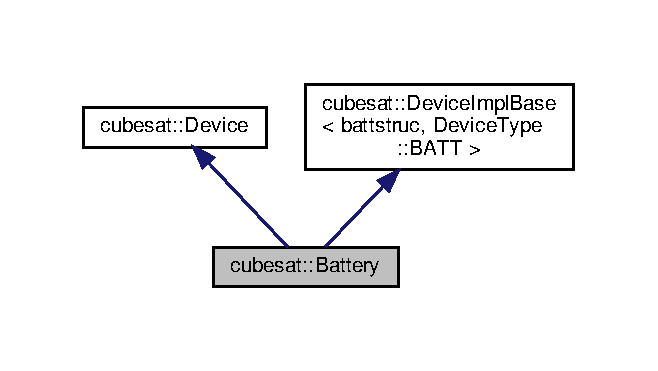
\includegraphics[width=316pt]{classcubesat_1_1Battery__inherit__graph}
\end{center}
\end{figure}


Collaboration diagram for cubesat\+:\+:Battery\+:
\nopagebreak
\begin{figure}[H]
\begin{center}
\leavevmode
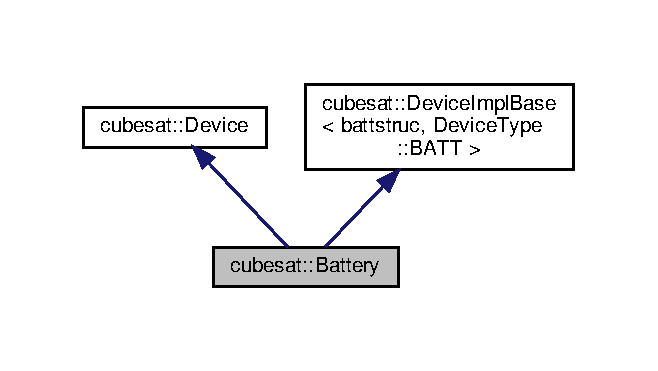
\includegraphics[width=316pt]{classcubesat_1_1Battery__coll__graph}
\end{center}
\end{figure}
\subsection*{Public Member Functions}
\begin{DoxyCompactItemize}
\item 
\hyperlink{classcubesat_1_1Battery_a2c27589782cfbb60129eb2a98a8ee0f4}{Battery} (Agent $\ast$\hyperlink{classcubesat_1_1Device_a8499108eccaf7375bea8ead0182391a6}{agent}, int \hyperlink{classcubesat_1_1Device_a1deca725b01f8ef37e49662da6db4e53}{cindex}, int \hyperlink{classcubesat_1_1Device_a8a2b3d6d7400e6796c31705058172982}{dindex})
\item 
virtual \hyperlink{classcubesat_1_1Battery_aa57aef1e0d1094eba5c7167156936607}{$\sim$\+Battery} ()
\item 
\hyperlink{classcubesat_1_1Battery_ad85cb4924badf1334a5f49edc8d5553c}{\+\_\+\+Add\+Property} (temperature, temp)
\item 
\hyperlink{classcubesat_1_1Battery_ace4f8ae340d704a56e2605792f084b57}{\+\_\+\+Add\+Property} (utc, utc)
\item 
\hyperlink{classcubesat_1_1Battery_a5c04c3be3f27e6476d1d36f95aebbc1a}{\+\_\+\+Add\+Property} (voltage, volt)
\item 
\hyperlink{classcubesat_1_1Battery_a0d8d177978d071aa3fb5012656fa2011}{\+\_\+\+Add\+Property} (current, amp)
\item 
\hyperlink{classcubesat_1_1Battery_a4141a2442d1b8f1dee5fb4925a11b17c}{\+\_\+\+Add\+Property} (power, power)
\item 
\hyperlink{classcubesat_1_1Battery_a9714a7dbbb19768ee8d2d1ea1b3011cd}{\+\_\+\+Add\+Property} (enabled, enabled)
\item 
\hyperlink{classcubesat_1_1Battery_a668dabc1438e3ad246e0d3168739a5ec}{\+\_\+\+Add\+Property} (percentage, percentage)
\item 
\hyperlink{classcubesat_1_1Battery_a2682885fce26c9b7d982b5ca57faaf17}{\+\_\+\+Add\+Property} (capacity, capacity)
\item 
\hyperlink{classcubesat_1_1Battery_ad81af4425073ae604a62d34a63f55506}{\+\_\+\+Add\+Property} (charge, charge)
\item 
\hyperlink{classcubesat_1_1Battery_a04d91c0ec695dfdedc33e5f3e4c74383}{\+\_\+\+Add\+Property} (efficiency, efficiency)
\item 
\hyperlink{classcubesat_1_1Battery_a0fb694ff309d0be2bbb1fc4d362c2984}{\+\_\+\+Add\+Property} (time\+\_\+remaining, time\+\_\+remaining)
\end{DoxyCompactItemize}
\subsection*{Additional Inherited Members}


\subsection{Constructor \& Destructor Documentation}
\mbox{\Hypertarget{classcubesat_1_1Battery_a2c27589782cfbb60129eb2a98a8ee0f4}\label{classcubesat_1_1Battery_a2c27589782cfbb60129eb2a98a8ee0f4}} 
\index{cubesat\+::\+Battery@{cubesat\+::\+Battery}!Battery@{Battery}}
\index{Battery@{Battery}!cubesat\+::\+Battery@{cubesat\+::\+Battery}}
\subsubsection{\texorpdfstring{Battery()}{Battery()}}
{\footnotesize\ttfamily cubesat\+::\+Battery\+::\+Battery (\begin{DoxyParamCaption}\item[{Agent $\ast$}]{agent,  }\item[{int}]{cindex,  }\item[{int}]{dindex }\end{DoxyParamCaption})\hspace{0.3cm}{\ttfamily [inline]}}

\mbox{\Hypertarget{classcubesat_1_1Battery_aa57aef1e0d1094eba5c7167156936607}\label{classcubesat_1_1Battery_aa57aef1e0d1094eba5c7167156936607}} 
\index{cubesat\+::\+Battery@{cubesat\+::\+Battery}!````~Battery@{$\sim$\+Battery}}
\index{````~Battery@{$\sim$\+Battery}!cubesat\+::\+Battery@{cubesat\+::\+Battery}}
\subsubsection{\texorpdfstring{$\sim$\+Battery()}{~Battery()}}
{\footnotesize\ttfamily virtual cubesat\+::\+Battery\+::$\sim$\+Battery (\begin{DoxyParamCaption}{ }\end{DoxyParamCaption})\hspace{0.3cm}{\ttfamily [inline]}, {\ttfamily [virtual]}}



\subsection{Member Function Documentation}
\mbox{\Hypertarget{classcubesat_1_1Battery_ad85cb4924badf1334a5f49edc8d5553c}\label{classcubesat_1_1Battery_ad85cb4924badf1334a5f49edc8d5553c}} 
\index{cubesat\+::\+Battery@{cubesat\+::\+Battery}!\+\_\+\+Add\+Property@{\+\_\+\+Add\+Property}}
\index{\+\_\+\+Add\+Property@{\+\_\+\+Add\+Property}!cubesat\+::\+Battery@{cubesat\+::\+Battery}}
\subsubsection{\texorpdfstring{\+\_\+\+Add\+Property()}{\_AddProperty()}\hspace{0.1cm}{\footnotesize\ttfamily [1/11]}}
{\footnotesize\ttfamily cubesat\+::\+Battery\+::\+\_\+\+Add\+Property (\begin{DoxyParamCaption}\item[{temperature}]{,  }\item[{temp}]{ }\end{DoxyParamCaption})}

\mbox{\Hypertarget{classcubesat_1_1Battery_ace4f8ae340d704a56e2605792f084b57}\label{classcubesat_1_1Battery_ace4f8ae340d704a56e2605792f084b57}} 
\index{cubesat\+::\+Battery@{cubesat\+::\+Battery}!\+\_\+\+Add\+Property@{\+\_\+\+Add\+Property}}
\index{\+\_\+\+Add\+Property@{\+\_\+\+Add\+Property}!cubesat\+::\+Battery@{cubesat\+::\+Battery}}
\subsubsection{\texorpdfstring{\+\_\+\+Add\+Property()}{\_AddProperty()}\hspace{0.1cm}{\footnotesize\ttfamily [2/11]}}
{\footnotesize\ttfamily cubesat\+::\+Battery\+::\+\_\+\+Add\+Property (\begin{DoxyParamCaption}\item[{utc}]{,  }\item[{utc}]{ }\end{DoxyParamCaption})}

\mbox{\Hypertarget{classcubesat_1_1Battery_a5c04c3be3f27e6476d1d36f95aebbc1a}\label{classcubesat_1_1Battery_a5c04c3be3f27e6476d1d36f95aebbc1a}} 
\index{cubesat\+::\+Battery@{cubesat\+::\+Battery}!\+\_\+\+Add\+Property@{\+\_\+\+Add\+Property}}
\index{\+\_\+\+Add\+Property@{\+\_\+\+Add\+Property}!cubesat\+::\+Battery@{cubesat\+::\+Battery}}
\subsubsection{\texorpdfstring{\+\_\+\+Add\+Property()}{\_AddProperty()}\hspace{0.1cm}{\footnotesize\ttfamily [3/11]}}
{\footnotesize\ttfamily cubesat\+::\+Battery\+::\+\_\+\+Add\+Property (\begin{DoxyParamCaption}\item[{voltage}]{,  }\item[{volt}]{ }\end{DoxyParamCaption})}

\mbox{\Hypertarget{classcubesat_1_1Battery_a0d8d177978d071aa3fb5012656fa2011}\label{classcubesat_1_1Battery_a0d8d177978d071aa3fb5012656fa2011}} 
\index{cubesat\+::\+Battery@{cubesat\+::\+Battery}!\+\_\+\+Add\+Property@{\+\_\+\+Add\+Property}}
\index{\+\_\+\+Add\+Property@{\+\_\+\+Add\+Property}!cubesat\+::\+Battery@{cubesat\+::\+Battery}}
\subsubsection{\texorpdfstring{\+\_\+\+Add\+Property()}{\_AddProperty()}\hspace{0.1cm}{\footnotesize\ttfamily [4/11]}}
{\footnotesize\ttfamily cubesat\+::\+Battery\+::\+\_\+\+Add\+Property (\begin{DoxyParamCaption}\item[{current}]{,  }\item[{amp}]{ }\end{DoxyParamCaption})}

\mbox{\Hypertarget{classcubesat_1_1Battery_a4141a2442d1b8f1dee5fb4925a11b17c}\label{classcubesat_1_1Battery_a4141a2442d1b8f1dee5fb4925a11b17c}} 
\index{cubesat\+::\+Battery@{cubesat\+::\+Battery}!\+\_\+\+Add\+Property@{\+\_\+\+Add\+Property}}
\index{\+\_\+\+Add\+Property@{\+\_\+\+Add\+Property}!cubesat\+::\+Battery@{cubesat\+::\+Battery}}
\subsubsection{\texorpdfstring{\+\_\+\+Add\+Property()}{\_AddProperty()}\hspace{0.1cm}{\footnotesize\ttfamily [5/11]}}
{\footnotesize\ttfamily cubesat\+::\+Battery\+::\+\_\+\+Add\+Property (\begin{DoxyParamCaption}\item[{power}]{,  }\item[{power}]{ }\end{DoxyParamCaption})}

\mbox{\Hypertarget{classcubesat_1_1Battery_a9714a7dbbb19768ee8d2d1ea1b3011cd}\label{classcubesat_1_1Battery_a9714a7dbbb19768ee8d2d1ea1b3011cd}} 
\index{cubesat\+::\+Battery@{cubesat\+::\+Battery}!\+\_\+\+Add\+Property@{\+\_\+\+Add\+Property}}
\index{\+\_\+\+Add\+Property@{\+\_\+\+Add\+Property}!cubesat\+::\+Battery@{cubesat\+::\+Battery}}
\subsubsection{\texorpdfstring{\+\_\+\+Add\+Property()}{\_AddProperty()}\hspace{0.1cm}{\footnotesize\ttfamily [6/11]}}
{\footnotesize\ttfamily cubesat\+::\+Battery\+::\+\_\+\+Add\+Property (\begin{DoxyParamCaption}\item[{enabled}]{,  }\item[{enabled}]{ }\end{DoxyParamCaption})}

\mbox{\Hypertarget{classcubesat_1_1Battery_a668dabc1438e3ad246e0d3168739a5ec}\label{classcubesat_1_1Battery_a668dabc1438e3ad246e0d3168739a5ec}} 
\index{cubesat\+::\+Battery@{cubesat\+::\+Battery}!\+\_\+\+Add\+Property@{\+\_\+\+Add\+Property}}
\index{\+\_\+\+Add\+Property@{\+\_\+\+Add\+Property}!cubesat\+::\+Battery@{cubesat\+::\+Battery}}
\subsubsection{\texorpdfstring{\+\_\+\+Add\+Property()}{\_AddProperty()}\hspace{0.1cm}{\footnotesize\ttfamily [7/11]}}
{\footnotesize\ttfamily cubesat\+::\+Battery\+::\+\_\+\+Add\+Property (\begin{DoxyParamCaption}\item[{percentage}]{,  }\item[{percentage}]{ }\end{DoxyParamCaption})}

\mbox{\Hypertarget{classcubesat_1_1Battery_a2682885fce26c9b7d982b5ca57faaf17}\label{classcubesat_1_1Battery_a2682885fce26c9b7d982b5ca57faaf17}} 
\index{cubesat\+::\+Battery@{cubesat\+::\+Battery}!\+\_\+\+Add\+Property@{\+\_\+\+Add\+Property}}
\index{\+\_\+\+Add\+Property@{\+\_\+\+Add\+Property}!cubesat\+::\+Battery@{cubesat\+::\+Battery}}
\subsubsection{\texorpdfstring{\+\_\+\+Add\+Property()}{\_AddProperty()}\hspace{0.1cm}{\footnotesize\ttfamily [8/11]}}
{\footnotesize\ttfamily cubesat\+::\+Battery\+::\+\_\+\+Add\+Property (\begin{DoxyParamCaption}\item[{capacity}]{,  }\item[{capacity}]{ }\end{DoxyParamCaption})}

\mbox{\Hypertarget{classcubesat_1_1Battery_ad81af4425073ae604a62d34a63f55506}\label{classcubesat_1_1Battery_ad81af4425073ae604a62d34a63f55506}} 
\index{cubesat\+::\+Battery@{cubesat\+::\+Battery}!\+\_\+\+Add\+Property@{\+\_\+\+Add\+Property}}
\index{\+\_\+\+Add\+Property@{\+\_\+\+Add\+Property}!cubesat\+::\+Battery@{cubesat\+::\+Battery}}
\subsubsection{\texorpdfstring{\+\_\+\+Add\+Property()}{\_AddProperty()}\hspace{0.1cm}{\footnotesize\ttfamily [9/11]}}
{\footnotesize\ttfamily cubesat\+::\+Battery\+::\+\_\+\+Add\+Property (\begin{DoxyParamCaption}\item[{charge}]{,  }\item[{charge}]{ }\end{DoxyParamCaption})}

\mbox{\Hypertarget{classcubesat_1_1Battery_a04d91c0ec695dfdedc33e5f3e4c74383}\label{classcubesat_1_1Battery_a04d91c0ec695dfdedc33e5f3e4c74383}} 
\index{cubesat\+::\+Battery@{cubesat\+::\+Battery}!\+\_\+\+Add\+Property@{\+\_\+\+Add\+Property}}
\index{\+\_\+\+Add\+Property@{\+\_\+\+Add\+Property}!cubesat\+::\+Battery@{cubesat\+::\+Battery}}
\subsubsection{\texorpdfstring{\+\_\+\+Add\+Property()}{\_AddProperty()}\hspace{0.1cm}{\footnotesize\ttfamily [10/11]}}
{\footnotesize\ttfamily cubesat\+::\+Battery\+::\+\_\+\+Add\+Property (\begin{DoxyParamCaption}\item[{efficiency}]{,  }\item[{efficiency}]{ }\end{DoxyParamCaption})}

\mbox{\Hypertarget{classcubesat_1_1Battery_a0fb694ff309d0be2bbb1fc4d362c2984}\label{classcubesat_1_1Battery_a0fb694ff309d0be2bbb1fc4d362c2984}} 
\index{cubesat\+::\+Battery@{cubesat\+::\+Battery}!\+\_\+\+Add\+Property@{\+\_\+\+Add\+Property}}
\index{\+\_\+\+Add\+Property@{\+\_\+\+Add\+Property}!cubesat\+::\+Battery@{cubesat\+::\+Battery}}
\subsubsection{\texorpdfstring{\+\_\+\+Add\+Property()}{\_AddProperty()}\hspace{0.1cm}{\footnotesize\ttfamily [11/11]}}
{\footnotesize\ttfamily cubesat\+::\+Battery\+::\+\_\+\+Add\+Property (\begin{DoxyParamCaption}\item[{time\+\_\+remaining}]{,  }\item[{time\+\_\+remaining}]{ }\end{DoxyParamCaption})}



The documentation for this class was generated from the following file\+:\begin{DoxyCompactItemize}
\item 
/home/osboxes/cosmos/source/projects/cubesat-\/kit/include/utility/\hyperlink{Device_8h}{Device.\+h}\end{DoxyCompactItemize}

\hypertarget{structcubesat_1_1Node_1_1BatteryCapacity}{}\section{cubesat\+:\+:Node\+:\+:Battery\+Capacity Struct Reference}
\label{structcubesat_1_1Node_1_1BatteryCapacity}\index{cubesat\+::\+Node\+::\+Battery\+Capacity@{cubesat\+::\+Node\+::\+Battery\+Capacity}}


{\ttfamily \#include $<$Device\+Detail.\+h$>$}



Inheritance diagram for cubesat\+:\+:Node\+:\+:Battery\+Capacity\+:
\nopagebreak
\begin{figure}[H]
\begin{center}
\leavevmode
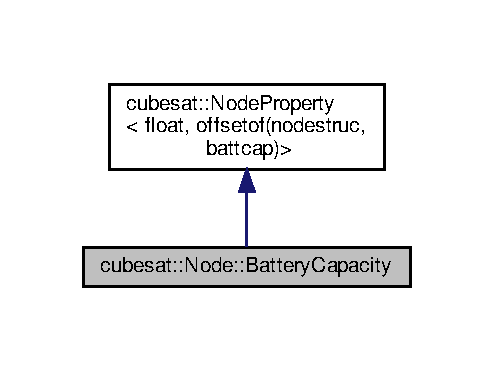
\includegraphics[width=237pt]{structcubesat_1_1Node_1_1BatteryCapacity__inherit__graph}
\end{center}
\end{figure}


Collaboration diagram for cubesat\+:\+:Node\+:\+:Battery\+Capacity\+:
\nopagebreak
\begin{figure}[H]
\begin{center}
\leavevmode
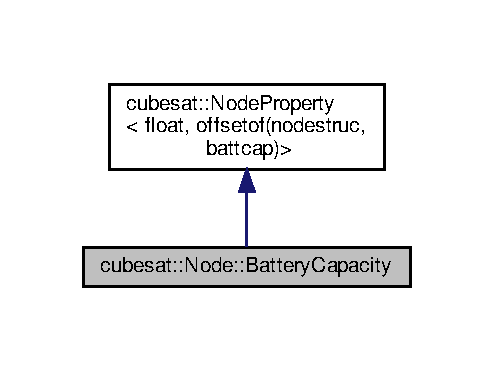
\includegraphics[width=237pt]{structcubesat_1_1Node_1_1BatteryCapacity__coll__graph}
\end{center}
\end{figure}
\subsection*{Static Public Attributes}
\begin{DoxyCompactItemize}
\item 
static constexpr auto \hyperlink{structcubesat_1_1Node_1_1BatteryCapacity_a2e14eaa079b2b98d34cc7f35f649ba1d}{key} = \char`\"{}node\+\_\+battcap\char`\"{}
\item 
static constexpr const char $\ast$ \hyperlink{structcubesat_1_1Node_1_1BatteryCapacity_a5e60db41b41d845dae7415be9eb258c7}{name} = \char`\"{}Battery Capacity\char`\"{}
\end{DoxyCompactItemize}
\subsection*{Additional Inherited Members}


\subsection{Member Data Documentation}
\mbox{\Hypertarget{structcubesat_1_1Node_1_1BatteryCapacity_a2e14eaa079b2b98d34cc7f35f649ba1d}\label{structcubesat_1_1Node_1_1BatteryCapacity_a2e14eaa079b2b98d34cc7f35f649ba1d}} 
\index{cubesat\+::\+Node\+::\+Battery\+Capacity@{cubesat\+::\+Node\+::\+Battery\+Capacity}!key@{key}}
\index{key@{key}!cubesat\+::\+Node\+::\+Battery\+Capacity@{cubesat\+::\+Node\+::\+Battery\+Capacity}}
\subsubsection{\texorpdfstring{key}{key}}
{\footnotesize\ttfamily constexpr auto cubesat\+::\+Node\+::\+Battery\+Capacity\+::key = \char`\"{}node\+\_\+battcap\char`\"{}\hspace{0.3cm}{\ttfamily [static]}}

\mbox{\Hypertarget{structcubesat_1_1Node_1_1BatteryCapacity_a5e60db41b41d845dae7415be9eb258c7}\label{structcubesat_1_1Node_1_1BatteryCapacity_a5e60db41b41d845dae7415be9eb258c7}} 
\index{cubesat\+::\+Node\+::\+Battery\+Capacity@{cubesat\+::\+Node\+::\+Battery\+Capacity}!name@{name}}
\index{name@{name}!cubesat\+::\+Node\+::\+Battery\+Capacity@{cubesat\+::\+Node\+::\+Battery\+Capacity}}
\subsubsection{\texorpdfstring{name}{name}}
{\footnotesize\ttfamily constexpr const char$\ast$ cubesat\+::\+Node\+::\+Battery\+Capacity\+::name = \char`\"{}Battery Capacity\char`\"{}\hspace{0.3cm}{\ttfamily [static]}}



The documentation for this struct was generated from the following file\+:\begin{DoxyCompactItemize}
\item 
/home/osboxes/cosmos/source/projects/cubesat-\/kit/include/utility/\hyperlink{DeviceDetail_8h}{Device\+Detail.\+h}\end{DoxyCompactItemize}

\hypertarget{structcubesat_1_1Node_1_1BatteryCharge}{}\section{cubesat\+:\+:Node\+:\+:Battery\+Charge Struct Reference}
\label{structcubesat_1_1Node_1_1BatteryCharge}\index{cubesat\+::\+Node\+::\+Battery\+Charge@{cubesat\+::\+Node\+::\+Battery\+Charge}}


{\ttfamily \#include $<$Device\+Detail.\+h$>$}



Inheritance diagram for cubesat\+:\+:Node\+:\+:Battery\+Charge\+:
\nopagebreak
\begin{figure}[H]
\begin{center}
\leavevmode
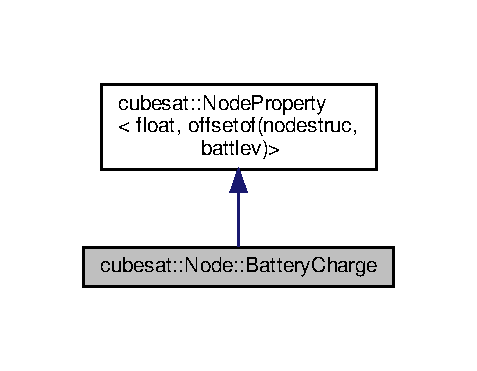
\includegraphics[width=229pt]{structcubesat_1_1Node_1_1BatteryCharge__inherit__graph}
\end{center}
\end{figure}


Collaboration diagram for cubesat\+:\+:Node\+:\+:Battery\+Charge\+:
\nopagebreak
\begin{figure}[H]
\begin{center}
\leavevmode
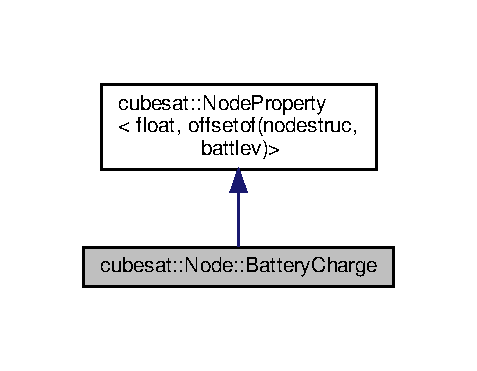
\includegraphics[width=229pt]{structcubesat_1_1Node_1_1BatteryCharge__coll__graph}
\end{center}
\end{figure}
\subsection*{Static Public Attributes}
\begin{DoxyCompactItemize}
\item 
static constexpr auto \hyperlink{structcubesat_1_1Node_1_1BatteryCharge_a587e3d823545b63cf86a1ebac8742605}{key} = \char`\"{}node\+\_\+battlev\char`\"{}
\item 
static constexpr const char $\ast$ \hyperlink{structcubesat_1_1Node_1_1BatteryCharge_a84060aceda01007b961d8beaca73fc41}{name} = \char`\"{}Battery Charge\char`\"{}
\end{DoxyCompactItemize}
\subsection*{Additional Inherited Members}


\subsection{Member Data Documentation}
\mbox{\Hypertarget{structcubesat_1_1Node_1_1BatteryCharge_a587e3d823545b63cf86a1ebac8742605}\label{structcubesat_1_1Node_1_1BatteryCharge_a587e3d823545b63cf86a1ebac8742605}} 
\index{cubesat\+::\+Node\+::\+Battery\+Charge@{cubesat\+::\+Node\+::\+Battery\+Charge}!key@{key}}
\index{key@{key}!cubesat\+::\+Node\+::\+Battery\+Charge@{cubesat\+::\+Node\+::\+Battery\+Charge}}
\subsubsection{\texorpdfstring{key}{key}}
{\footnotesize\ttfamily constexpr auto cubesat\+::\+Node\+::\+Battery\+Charge\+::key = \char`\"{}node\+\_\+battlev\char`\"{}\hspace{0.3cm}{\ttfamily [static]}}

\mbox{\Hypertarget{structcubesat_1_1Node_1_1BatteryCharge_a84060aceda01007b961d8beaca73fc41}\label{structcubesat_1_1Node_1_1BatteryCharge_a84060aceda01007b961d8beaca73fc41}} 
\index{cubesat\+::\+Node\+::\+Battery\+Charge@{cubesat\+::\+Node\+::\+Battery\+Charge}!name@{name}}
\index{name@{name}!cubesat\+::\+Node\+::\+Battery\+Charge@{cubesat\+::\+Node\+::\+Battery\+Charge}}
\subsubsection{\texorpdfstring{name}{name}}
{\footnotesize\ttfamily constexpr const char$\ast$ cubesat\+::\+Node\+::\+Battery\+Charge\+::name = \char`\"{}Battery Charge\char`\"{}\hspace{0.3cm}{\ttfamily [static]}}



The documentation for this struct was generated from the following file\+:\begin{DoxyCompactItemize}
\item 
/home/osboxes/cosmos/source/projects/cubesat-\/kit/include/utility/\hyperlink{DeviceDetail_8h}{Device\+Detail.\+h}\end{DoxyCompactItemize}

\hypertarget{classcubesat_1_1Camera}{}\section{cubesat\+:\+:Camera Class Reference}
\label{classcubesat_1_1Camera}\index{cubesat\+::\+Camera@{cubesat\+::\+Camera}}


{\ttfamily \#include $<$Device.\+h$>$}



Inheritance diagram for cubesat\+:\+:Camera\+:
\nopagebreak
\begin{figure}[H]
\begin{center}
\leavevmode
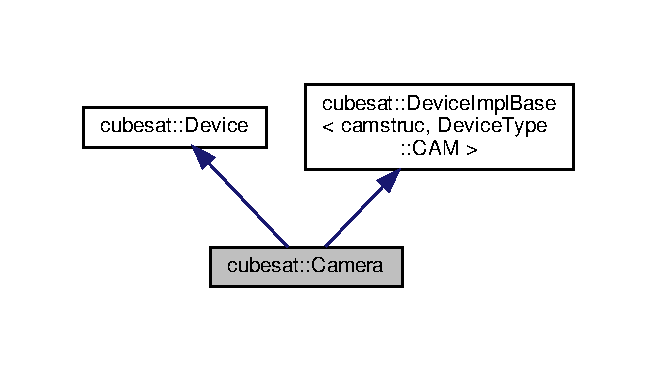
\includegraphics[width=316pt]{classcubesat_1_1Camera__inherit__graph}
\end{center}
\end{figure}


Collaboration diagram for cubesat\+:\+:Camera\+:
\nopagebreak
\begin{figure}[H]
\begin{center}
\leavevmode
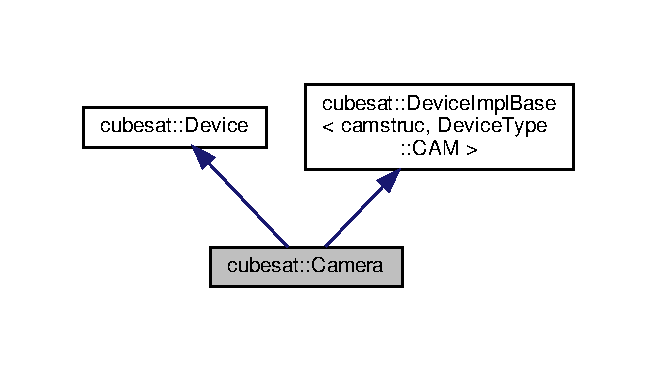
\includegraphics[width=316pt]{classcubesat_1_1Camera__coll__graph}
\end{center}
\end{figure}
\subsection*{Public Member Functions}
\begin{DoxyCompactItemize}
\item 
\hyperlink{classcubesat_1_1Camera_ae1731bde4ac0f35492e17b1319c4840e}{Camera} (Agent $\ast$\hyperlink{classcubesat_1_1Device_a8499108eccaf7375bea8ead0182391a6}{agent}, int \hyperlink{classcubesat_1_1Device_a1deca725b01f8ef37e49662da6db4e53}{cindex}, int \hyperlink{classcubesat_1_1Device_a8a2b3d6d7400e6796c31705058172982}{dindex})
\item 
virtual \hyperlink{classcubesat_1_1Camera_a8341dc6e32e8578a75e6fbe9ed6d1234}{$\sim$\+Camera} ()
\item 
\hyperlink{classcubesat_1_1Camera_a4f716ff4fcce35b24596c0b81c103efb}{\+\_\+\+Add\+Property} (temperature, temp)
\item 
\hyperlink{classcubesat_1_1Camera_a2f84cf3b74e6c46765c5b557d72bd39c}{\+\_\+\+Add\+Property} (utc, utc)
\item 
\hyperlink{classcubesat_1_1Camera_a849d2605913ca6f995b79d90dd260db6}{\+\_\+\+Add\+Property} (voltage, volt)
\item 
\hyperlink{classcubesat_1_1Camera_a2586b6fceabbf85db5842e6e16351b93}{\+\_\+\+Add\+Property} (current, amp)
\item 
\hyperlink{classcubesat_1_1Camera_a0465aa58841962ef8be4e8c5523194ec}{\+\_\+\+Add\+Property} (power, power)
\item 
\hyperlink{classcubesat_1_1Camera_afa9900e8a42e4b91f82e7bf005e6c28d}{\+\_\+\+Add\+Property} (enabled, enabled)
\item 
\hyperlink{classcubesat_1_1Camera_af54a43e0cf808c26f32c8b8096ebc3f7}{\+\_\+\+Add\+Property} (pixel\+\_\+width, pwidth)
\item 
\hyperlink{classcubesat_1_1Camera_a29cd2ba4b65f32cb43e7e96fe242d258}{\+\_\+\+Add\+Property} (pixel\+\_\+height, pheight)
\item 
\hyperlink{classcubesat_1_1Camera_aad0910a49f04446c5f5266b37262692e}{\+\_\+\+Add\+Property} (width, width)
\item 
\hyperlink{classcubesat_1_1Camera_aeed37c12ee4119bf54fc7124fba19b97}{\+\_\+\+Add\+Property} (height, height)
\item 
\hyperlink{classcubesat_1_1Camera_a136f46ab3e38b076adba6c4d718a80ab}{\+\_\+\+Add\+Property} (focal\+\_\+length, flength)
\end{DoxyCompactItemize}
\subsection*{Additional Inherited Members}


\subsection{Constructor \& Destructor Documentation}
\mbox{\Hypertarget{classcubesat_1_1Camera_ae1731bde4ac0f35492e17b1319c4840e}\label{classcubesat_1_1Camera_ae1731bde4ac0f35492e17b1319c4840e}} 
\index{cubesat\+::\+Camera@{cubesat\+::\+Camera}!Camera@{Camera}}
\index{Camera@{Camera}!cubesat\+::\+Camera@{cubesat\+::\+Camera}}
\subsubsection{\texorpdfstring{Camera()}{Camera()}}
{\footnotesize\ttfamily cubesat\+::\+Camera\+::\+Camera (\begin{DoxyParamCaption}\item[{Agent $\ast$}]{agent,  }\item[{int}]{cindex,  }\item[{int}]{dindex }\end{DoxyParamCaption})\hspace{0.3cm}{\ttfamily [inline]}}

\mbox{\Hypertarget{classcubesat_1_1Camera_a8341dc6e32e8578a75e6fbe9ed6d1234}\label{classcubesat_1_1Camera_a8341dc6e32e8578a75e6fbe9ed6d1234}} 
\index{cubesat\+::\+Camera@{cubesat\+::\+Camera}!````~Camera@{$\sim$\+Camera}}
\index{````~Camera@{$\sim$\+Camera}!cubesat\+::\+Camera@{cubesat\+::\+Camera}}
\subsubsection{\texorpdfstring{$\sim$\+Camera()}{~Camera()}}
{\footnotesize\ttfamily virtual cubesat\+::\+Camera\+::$\sim$\+Camera (\begin{DoxyParamCaption}{ }\end{DoxyParamCaption})\hspace{0.3cm}{\ttfamily [inline]}, {\ttfamily [virtual]}}



\subsection{Member Function Documentation}
\mbox{\Hypertarget{classcubesat_1_1Camera_a4f716ff4fcce35b24596c0b81c103efb}\label{classcubesat_1_1Camera_a4f716ff4fcce35b24596c0b81c103efb}} 
\index{cubesat\+::\+Camera@{cubesat\+::\+Camera}!\+\_\+\+Add\+Property@{\+\_\+\+Add\+Property}}
\index{\+\_\+\+Add\+Property@{\+\_\+\+Add\+Property}!cubesat\+::\+Camera@{cubesat\+::\+Camera}}
\subsubsection{\texorpdfstring{\+\_\+\+Add\+Property()}{\_AddProperty()}\hspace{0.1cm}{\footnotesize\ttfamily [1/11]}}
{\footnotesize\ttfamily cubesat\+::\+Camera\+::\+\_\+\+Add\+Property (\begin{DoxyParamCaption}\item[{temperature}]{,  }\item[{temp}]{ }\end{DoxyParamCaption})}

\mbox{\Hypertarget{classcubesat_1_1Camera_a2f84cf3b74e6c46765c5b557d72bd39c}\label{classcubesat_1_1Camera_a2f84cf3b74e6c46765c5b557d72bd39c}} 
\index{cubesat\+::\+Camera@{cubesat\+::\+Camera}!\+\_\+\+Add\+Property@{\+\_\+\+Add\+Property}}
\index{\+\_\+\+Add\+Property@{\+\_\+\+Add\+Property}!cubesat\+::\+Camera@{cubesat\+::\+Camera}}
\subsubsection{\texorpdfstring{\+\_\+\+Add\+Property()}{\_AddProperty()}\hspace{0.1cm}{\footnotesize\ttfamily [2/11]}}
{\footnotesize\ttfamily cubesat\+::\+Camera\+::\+\_\+\+Add\+Property (\begin{DoxyParamCaption}\item[{utc}]{,  }\item[{utc}]{ }\end{DoxyParamCaption})}

\mbox{\Hypertarget{classcubesat_1_1Camera_a849d2605913ca6f995b79d90dd260db6}\label{classcubesat_1_1Camera_a849d2605913ca6f995b79d90dd260db6}} 
\index{cubesat\+::\+Camera@{cubesat\+::\+Camera}!\+\_\+\+Add\+Property@{\+\_\+\+Add\+Property}}
\index{\+\_\+\+Add\+Property@{\+\_\+\+Add\+Property}!cubesat\+::\+Camera@{cubesat\+::\+Camera}}
\subsubsection{\texorpdfstring{\+\_\+\+Add\+Property()}{\_AddProperty()}\hspace{0.1cm}{\footnotesize\ttfamily [3/11]}}
{\footnotesize\ttfamily cubesat\+::\+Camera\+::\+\_\+\+Add\+Property (\begin{DoxyParamCaption}\item[{voltage}]{,  }\item[{volt}]{ }\end{DoxyParamCaption})}

\mbox{\Hypertarget{classcubesat_1_1Camera_a2586b6fceabbf85db5842e6e16351b93}\label{classcubesat_1_1Camera_a2586b6fceabbf85db5842e6e16351b93}} 
\index{cubesat\+::\+Camera@{cubesat\+::\+Camera}!\+\_\+\+Add\+Property@{\+\_\+\+Add\+Property}}
\index{\+\_\+\+Add\+Property@{\+\_\+\+Add\+Property}!cubesat\+::\+Camera@{cubesat\+::\+Camera}}
\subsubsection{\texorpdfstring{\+\_\+\+Add\+Property()}{\_AddProperty()}\hspace{0.1cm}{\footnotesize\ttfamily [4/11]}}
{\footnotesize\ttfamily cubesat\+::\+Camera\+::\+\_\+\+Add\+Property (\begin{DoxyParamCaption}\item[{current}]{,  }\item[{amp}]{ }\end{DoxyParamCaption})}

\mbox{\Hypertarget{classcubesat_1_1Camera_a0465aa58841962ef8be4e8c5523194ec}\label{classcubesat_1_1Camera_a0465aa58841962ef8be4e8c5523194ec}} 
\index{cubesat\+::\+Camera@{cubesat\+::\+Camera}!\+\_\+\+Add\+Property@{\+\_\+\+Add\+Property}}
\index{\+\_\+\+Add\+Property@{\+\_\+\+Add\+Property}!cubesat\+::\+Camera@{cubesat\+::\+Camera}}
\subsubsection{\texorpdfstring{\+\_\+\+Add\+Property()}{\_AddProperty()}\hspace{0.1cm}{\footnotesize\ttfamily [5/11]}}
{\footnotesize\ttfamily cubesat\+::\+Camera\+::\+\_\+\+Add\+Property (\begin{DoxyParamCaption}\item[{power}]{,  }\item[{power}]{ }\end{DoxyParamCaption})}

\mbox{\Hypertarget{classcubesat_1_1Camera_afa9900e8a42e4b91f82e7bf005e6c28d}\label{classcubesat_1_1Camera_afa9900e8a42e4b91f82e7bf005e6c28d}} 
\index{cubesat\+::\+Camera@{cubesat\+::\+Camera}!\+\_\+\+Add\+Property@{\+\_\+\+Add\+Property}}
\index{\+\_\+\+Add\+Property@{\+\_\+\+Add\+Property}!cubesat\+::\+Camera@{cubesat\+::\+Camera}}
\subsubsection{\texorpdfstring{\+\_\+\+Add\+Property()}{\_AddProperty()}\hspace{0.1cm}{\footnotesize\ttfamily [6/11]}}
{\footnotesize\ttfamily cubesat\+::\+Camera\+::\+\_\+\+Add\+Property (\begin{DoxyParamCaption}\item[{enabled}]{,  }\item[{enabled}]{ }\end{DoxyParamCaption})}

\mbox{\Hypertarget{classcubesat_1_1Camera_af54a43e0cf808c26f32c8b8096ebc3f7}\label{classcubesat_1_1Camera_af54a43e0cf808c26f32c8b8096ebc3f7}} 
\index{cubesat\+::\+Camera@{cubesat\+::\+Camera}!\+\_\+\+Add\+Property@{\+\_\+\+Add\+Property}}
\index{\+\_\+\+Add\+Property@{\+\_\+\+Add\+Property}!cubesat\+::\+Camera@{cubesat\+::\+Camera}}
\subsubsection{\texorpdfstring{\+\_\+\+Add\+Property()}{\_AddProperty()}\hspace{0.1cm}{\footnotesize\ttfamily [7/11]}}
{\footnotesize\ttfamily cubesat\+::\+Camera\+::\+\_\+\+Add\+Property (\begin{DoxyParamCaption}\item[{pixel\+\_\+width}]{,  }\item[{pwidth}]{ }\end{DoxyParamCaption})}

\mbox{\Hypertarget{classcubesat_1_1Camera_a29cd2ba4b65f32cb43e7e96fe242d258}\label{classcubesat_1_1Camera_a29cd2ba4b65f32cb43e7e96fe242d258}} 
\index{cubesat\+::\+Camera@{cubesat\+::\+Camera}!\+\_\+\+Add\+Property@{\+\_\+\+Add\+Property}}
\index{\+\_\+\+Add\+Property@{\+\_\+\+Add\+Property}!cubesat\+::\+Camera@{cubesat\+::\+Camera}}
\subsubsection{\texorpdfstring{\+\_\+\+Add\+Property()}{\_AddProperty()}\hspace{0.1cm}{\footnotesize\ttfamily [8/11]}}
{\footnotesize\ttfamily cubesat\+::\+Camera\+::\+\_\+\+Add\+Property (\begin{DoxyParamCaption}\item[{pixel\+\_\+height}]{,  }\item[{pheight}]{ }\end{DoxyParamCaption})}

\mbox{\Hypertarget{classcubesat_1_1Camera_aad0910a49f04446c5f5266b37262692e}\label{classcubesat_1_1Camera_aad0910a49f04446c5f5266b37262692e}} 
\index{cubesat\+::\+Camera@{cubesat\+::\+Camera}!\+\_\+\+Add\+Property@{\+\_\+\+Add\+Property}}
\index{\+\_\+\+Add\+Property@{\+\_\+\+Add\+Property}!cubesat\+::\+Camera@{cubesat\+::\+Camera}}
\subsubsection{\texorpdfstring{\+\_\+\+Add\+Property()}{\_AddProperty()}\hspace{0.1cm}{\footnotesize\ttfamily [9/11]}}
{\footnotesize\ttfamily cubesat\+::\+Camera\+::\+\_\+\+Add\+Property (\begin{DoxyParamCaption}\item[{width}]{,  }\item[{width}]{ }\end{DoxyParamCaption})}

\mbox{\Hypertarget{classcubesat_1_1Camera_aeed37c12ee4119bf54fc7124fba19b97}\label{classcubesat_1_1Camera_aeed37c12ee4119bf54fc7124fba19b97}} 
\index{cubesat\+::\+Camera@{cubesat\+::\+Camera}!\+\_\+\+Add\+Property@{\+\_\+\+Add\+Property}}
\index{\+\_\+\+Add\+Property@{\+\_\+\+Add\+Property}!cubesat\+::\+Camera@{cubesat\+::\+Camera}}
\subsubsection{\texorpdfstring{\+\_\+\+Add\+Property()}{\_AddProperty()}\hspace{0.1cm}{\footnotesize\ttfamily [10/11]}}
{\footnotesize\ttfamily cubesat\+::\+Camera\+::\+\_\+\+Add\+Property (\begin{DoxyParamCaption}\item[{height}]{,  }\item[{height}]{ }\end{DoxyParamCaption})}

\mbox{\Hypertarget{classcubesat_1_1Camera_a136f46ab3e38b076adba6c4d718a80ab}\label{classcubesat_1_1Camera_a136f46ab3e38b076adba6c4d718a80ab}} 
\index{cubesat\+::\+Camera@{cubesat\+::\+Camera}!\+\_\+\+Add\+Property@{\+\_\+\+Add\+Property}}
\index{\+\_\+\+Add\+Property@{\+\_\+\+Add\+Property}!cubesat\+::\+Camera@{cubesat\+::\+Camera}}
\subsubsection{\texorpdfstring{\+\_\+\+Add\+Property()}{\_AddProperty()}\hspace{0.1cm}{\footnotesize\ttfamily [11/11]}}
{\footnotesize\ttfamily cubesat\+::\+Camera\+::\+\_\+\+Add\+Property (\begin{DoxyParamCaption}\item[{focal\+\_\+length}]{,  }\item[{flength}]{ }\end{DoxyParamCaption})}



The documentation for this class was generated from the following file\+:\begin{DoxyCompactItemize}
\item 
/home/osboxes/cosmos/source/projects/cubesat-\/kit/include/utility/\hyperlink{Device_8h}{Device.\+h}\end{DoxyCompactItemize}

\hypertarget{classcubesat_1_1ChipSelect}{}\section{cubesat\+:\+:Chip\+Select Class Reference}
\label{classcubesat_1_1ChipSelect}\index{cubesat\+::\+Chip\+Select@{cubesat\+::\+Chip\+Select}}


{\ttfamily \#include $<$Chip\+Select.\+h$>$}

\subsection*{Public Member Functions}
\begin{DoxyCompactItemize}
\item 
\hyperlink{classcubesat_1_1ChipSelect_a18fb93813dc66313c0ebdea468f61366}{Chip\+Select} (const std\+::vector$<$ std\+::string $>$ \&\hyperlink{classcubesat_1_1ChipSelect_ae6285a5edb25a1dbecce248bf1ac241d}{cs\+\_\+pin\+\_\+keys})
\begin{DoxyCompactList}\small\item\em Creates a \hyperlink{classcubesat_1_1ChipSelect}{Chip\+Select} object. \end{DoxyCompactList}\item 
void \hyperlink{classcubesat_1_1ChipSelect_ab173c06bea583f833b11bae2a305701d}{Acquire} (unsigned int address)
\begin{DoxyCompactList}\small\item\em Selects a chip at the given address. \end{DoxyCompactList}\end{DoxyCompactItemize}
\subsection*{Private Attributes}
\begin{DoxyCompactItemize}
\item 
std\+::vector$<$ std\+::string $>$ \hyperlink{classcubesat_1_1ChipSelect_ae6285a5edb25a1dbecce248bf1ac241d}{cs\+\_\+pin\+\_\+keys}
\begin{DoxyCompactList}\small\item\em The Beagle\+Bone \hyperlink{classcubesat_1_1GPIO}{G\+P\+IO} pin keys (e.\+g. P9\+\_\+14) \end{DoxyCompactList}\item 
std\+::vector$<$ \hyperlink{classcubesat_1_1GPIO}{G\+P\+IO} $>$ \hyperlink{classcubesat_1_1ChipSelect_a549f890313f33099ac514679d86501a4}{cs\+\_\+gpios}
\begin{DoxyCompactList}\small\item\em The Beagle\+Bone G\+P\+I\+Os. \end{DoxyCompactList}\end{DoxyCompactItemize}


\subsection{Constructor \& Destructor Documentation}
\mbox{\Hypertarget{classcubesat_1_1ChipSelect_a18fb93813dc66313c0ebdea468f61366}\label{classcubesat_1_1ChipSelect_a18fb93813dc66313c0ebdea468f61366}} 
\index{cubesat\+::\+Chip\+Select@{cubesat\+::\+Chip\+Select}!Chip\+Select@{Chip\+Select}}
\index{Chip\+Select@{Chip\+Select}!cubesat\+::\+Chip\+Select@{cubesat\+::\+Chip\+Select}}
\subsubsection{\texorpdfstring{Chip\+Select()}{ChipSelect()}}
{\footnotesize\ttfamily cubesat\+::\+Chip\+Select\+::\+Chip\+Select (\begin{DoxyParamCaption}\item[{const std\+::vector$<$ std\+::string $>$ \&}]{cs\+\_\+pin\+\_\+keys }\end{DoxyParamCaption})\hspace{0.3cm}{\ttfamily [inline]}}



Creates a \hyperlink{classcubesat_1_1ChipSelect}{Chip\+Select} object. 


\begin{DoxyParams}{Parameters}
{\em cs\+\_\+pin\+\_\+keys} & The pin keys, stored in big endian order \\
\hline
\end{DoxyParams}


\subsection{Member Function Documentation}
\mbox{\Hypertarget{classcubesat_1_1ChipSelect_ab173c06bea583f833b11bae2a305701d}\label{classcubesat_1_1ChipSelect_ab173c06bea583f833b11bae2a305701d}} 
\index{cubesat\+::\+Chip\+Select@{cubesat\+::\+Chip\+Select}!Acquire@{Acquire}}
\index{Acquire@{Acquire}!cubesat\+::\+Chip\+Select@{cubesat\+::\+Chip\+Select}}
\subsubsection{\texorpdfstring{Acquire()}{Acquire()}}
{\footnotesize\ttfamily void cubesat\+::\+Chip\+Select\+::\+Acquire (\begin{DoxyParamCaption}\item[{unsigned int}]{address }\end{DoxyParamCaption})\hspace{0.3cm}{\ttfamily [inline]}}



Selects a chip at the given address. 


\begin{DoxyParams}{Parameters}
{\em address} & The address (big endian) \\
\hline
\end{DoxyParams}


\subsection{Member Data Documentation}
\mbox{\Hypertarget{classcubesat_1_1ChipSelect_a549f890313f33099ac514679d86501a4}\label{classcubesat_1_1ChipSelect_a549f890313f33099ac514679d86501a4}} 
\index{cubesat\+::\+Chip\+Select@{cubesat\+::\+Chip\+Select}!cs\+\_\+gpios@{cs\+\_\+gpios}}
\index{cs\+\_\+gpios@{cs\+\_\+gpios}!cubesat\+::\+Chip\+Select@{cubesat\+::\+Chip\+Select}}
\subsubsection{\texorpdfstring{cs\+\_\+gpios}{cs\_gpios}}
{\footnotesize\ttfamily std\+::vector$<$\hyperlink{classcubesat_1_1GPIO}{G\+P\+IO}$>$ cubesat\+::\+Chip\+Select\+::cs\+\_\+gpios\hspace{0.3cm}{\ttfamily [private]}}



The Beagle\+Bone G\+P\+I\+Os. 

\mbox{\Hypertarget{classcubesat_1_1ChipSelect_ae6285a5edb25a1dbecce248bf1ac241d}\label{classcubesat_1_1ChipSelect_ae6285a5edb25a1dbecce248bf1ac241d}} 
\index{cubesat\+::\+Chip\+Select@{cubesat\+::\+Chip\+Select}!cs\+\_\+pin\+\_\+keys@{cs\+\_\+pin\+\_\+keys}}
\index{cs\+\_\+pin\+\_\+keys@{cs\+\_\+pin\+\_\+keys}!cubesat\+::\+Chip\+Select@{cubesat\+::\+Chip\+Select}}
\subsubsection{\texorpdfstring{cs\+\_\+pin\+\_\+keys}{cs\_pin\_keys}}
{\footnotesize\ttfamily std\+::vector$<$std\+::string$>$ cubesat\+::\+Chip\+Select\+::cs\+\_\+pin\+\_\+keys\hspace{0.3cm}{\ttfamily [private]}}



The Beagle\+Bone \hyperlink{classcubesat_1_1GPIO}{G\+P\+IO} pin keys (e.\+g. P9\+\_\+14) 



The documentation for this class was generated from the following file\+:\begin{DoxyCompactItemize}
\item 
/home/osboxes/cosmos/source/projects/cubesat-\/kit/include/device/\hyperlink{ChipSelect_8h}{Chip\+Select.\+h}\end{DoxyCompactItemize}

\hypertarget{unioncubesat_1_1OPT3001_1_1Configuration}{}\section{cubesat\+:\+:O\+P\+T3001\+:\+:Configuration Union Reference}
\label{unioncubesat_1_1OPT3001_1_1Configuration}\index{cubesat\+::\+O\+P\+T3001\+::\+Configuration@{cubesat\+::\+O\+P\+T3001\+::\+Configuration}}


\hyperlink{unioncubesat_1_1OPT3001_1_1Configuration}{Configuration} flags corresponding to the configuration register on the device.  




{\ttfamily \#include $<$O\+P\+T3001.\+h$>$}

\subsection*{Public Attributes}
\begin{DoxyCompactItemize}
\item 
\begin{tabbing}
xx\=xx\=xx\=xx\=xx\=xx\=xx\=xx\=xx\=\kill
struct \{\\
\>uint8\_t \hyperlink{unioncubesat_1_1OPT3001_1_1Configuration_aba3ee5b0e9c2a28707cec7979287da18}{FaultCount}: 2\\
\>uint8\_t \hyperlink{unioncubesat_1_1OPT3001_1_1Configuration_a0b7f2e67d9103f03a9c5ac1d787edaae}{MaskExponent}: 1\\
\>uint8\_t \hyperlink{unioncubesat_1_1OPT3001_1_1Configuration_a9be11aa37945c839ecbdbb82b110306c}{Polarity}: 1\\
\>uint8\_t \hyperlink{unioncubesat_1_1OPT3001_1_1Configuration_ab7abbbb5c58ffcc98b43e820e17580dd}{Latch}: 1\\
\>uint8\_t \hyperlink{unioncubesat_1_1OPT3001_1_1Configuration_a4e210133a90a7bbdf90273cfa53d4c6b}{FlagLow}: 1\\
\>uint8\_t \hyperlink{unioncubesat_1_1OPT3001_1_1Configuration_a6a4c40221beb13c4d839bc290849f2e8}{FlagHigh}: 1\\
\>uint8\_t \hyperlink{unioncubesat_1_1OPT3001_1_1Configuration_a1aca1b929f8e213896685d1981c8fe4a}{ConversionReady}: 1\\
\>uint8\_t \hyperlink{unioncubesat_1_1OPT3001_1_1Configuration_a5515ab2a3c0910b2f4df52ecc533527c}{OverflowFlag}: 1\\
\>uint8\_t \hyperlink{unioncubesat_1_1OPT3001_1_1Configuration_a18d5dc05b1f00f195631034d66fa46d1}{ModeOfConversionOperation}: 2\\
\>uint8\_t \hyperlink{unioncubesat_1_1OPT3001_1_1Configuration_ab978a7d7505ad3a69112c6cd437b595e}{ConversionTime}: 1\\
\>uint8\_t \hyperlink{unioncubesat_1_1OPT3001_1_1Configuration_a2f55f001b9254f9937781848c3354d9e}{RangeNumber}: 4\\
\}; \\

\end{tabbing}\item 
uint16\+\_\+t \hyperlink{unioncubesat_1_1OPT3001_1_1Configuration_a0ff485276b8cd27662ad0331e3c54b5b}{raw\+\_\+data}
\end{DoxyCompactItemize}


\subsection{Detailed Description}
\hyperlink{unioncubesat_1_1OPT3001_1_1Configuration}{Configuration} flags corresponding to the configuration register on the device. 

\subsection{Member Data Documentation}
\mbox{\Hypertarget{unioncubesat_1_1OPT3001_1_1Configuration_a0d4a4f269f0d67a8e73a15af42747aa7}\label{unioncubesat_1_1OPT3001_1_1Configuration_a0d4a4f269f0d67a8e73a15af42747aa7}} 
\subsubsection{\texorpdfstring{"@9}{@9}}
{\footnotesize\ttfamily struct \{ ... \} }

\mbox{\Hypertarget{unioncubesat_1_1OPT3001_1_1Configuration_a1aca1b929f8e213896685d1981c8fe4a}\label{unioncubesat_1_1OPT3001_1_1Configuration_a1aca1b929f8e213896685d1981c8fe4a}} 
\index{cubesat\+::\+O\+P\+T3001\+::\+Configuration@{cubesat\+::\+O\+P\+T3001\+::\+Configuration}!Conversion\+Ready@{Conversion\+Ready}}
\index{Conversion\+Ready@{Conversion\+Ready}!cubesat\+::\+O\+P\+T3001\+::\+Configuration@{cubesat\+::\+O\+P\+T3001\+::\+Configuration}}
\subsubsection{\texorpdfstring{Conversion\+Ready}{ConversionReady}}
{\footnotesize\ttfamily uint8\+\_\+t cubesat\+::\+O\+P\+T3001\+::\+Configuration\+::\+Conversion\+Ready}

\mbox{\Hypertarget{unioncubesat_1_1OPT3001_1_1Configuration_ab978a7d7505ad3a69112c6cd437b595e}\label{unioncubesat_1_1OPT3001_1_1Configuration_ab978a7d7505ad3a69112c6cd437b595e}} 
\index{cubesat\+::\+O\+P\+T3001\+::\+Configuration@{cubesat\+::\+O\+P\+T3001\+::\+Configuration}!Conversion\+Time@{Conversion\+Time}}
\index{Conversion\+Time@{Conversion\+Time}!cubesat\+::\+O\+P\+T3001\+::\+Configuration@{cubesat\+::\+O\+P\+T3001\+::\+Configuration}}
\subsubsection{\texorpdfstring{Conversion\+Time}{ConversionTime}}
{\footnotesize\ttfamily uint8\+\_\+t cubesat\+::\+O\+P\+T3001\+::\+Configuration\+::\+Conversion\+Time}

\mbox{\Hypertarget{unioncubesat_1_1OPT3001_1_1Configuration_aba3ee5b0e9c2a28707cec7979287da18}\label{unioncubesat_1_1OPT3001_1_1Configuration_aba3ee5b0e9c2a28707cec7979287da18}} 
\index{cubesat\+::\+O\+P\+T3001\+::\+Configuration@{cubesat\+::\+O\+P\+T3001\+::\+Configuration}!Fault\+Count@{Fault\+Count}}
\index{Fault\+Count@{Fault\+Count}!cubesat\+::\+O\+P\+T3001\+::\+Configuration@{cubesat\+::\+O\+P\+T3001\+::\+Configuration}}
\subsubsection{\texorpdfstring{Fault\+Count}{FaultCount}}
{\footnotesize\ttfamily uint8\+\_\+t cubesat\+::\+O\+P\+T3001\+::\+Configuration\+::\+Fault\+Count}

\mbox{\Hypertarget{unioncubesat_1_1OPT3001_1_1Configuration_a6a4c40221beb13c4d839bc290849f2e8}\label{unioncubesat_1_1OPT3001_1_1Configuration_a6a4c40221beb13c4d839bc290849f2e8}} 
\index{cubesat\+::\+O\+P\+T3001\+::\+Configuration@{cubesat\+::\+O\+P\+T3001\+::\+Configuration}!Flag\+High@{Flag\+High}}
\index{Flag\+High@{Flag\+High}!cubesat\+::\+O\+P\+T3001\+::\+Configuration@{cubesat\+::\+O\+P\+T3001\+::\+Configuration}}
\subsubsection{\texorpdfstring{Flag\+High}{FlagHigh}}
{\footnotesize\ttfamily uint8\+\_\+t cubesat\+::\+O\+P\+T3001\+::\+Configuration\+::\+Flag\+High}

\mbox{\Hypertarget{unioncubesat_1_1OPT3001_1_1Configuration_a4e210133a90a7bbdf90273cfa53d4c6b}\label{unioncubesat_1_1OPT3001_1_1Configuration_a4e210133a90a7bbdf90273cfa53d4c6b}} 
\index{cubesat\+::\+O\+P\+T3001\+::\+Configuration@{cubesat\+::\+O\+P\+T3001\+::\+Configuration}!Flag\+Low@{Flag\+Low}}
\index{Flag\+Low@{Flag\+Low}!cubesat\+::\+O\+P\+T3001\+::\+Configuration@{cubesat\+::\+O\+P\+T3001\+::\+Configuration}}
\subsubsection{\texorpdfstring{Flag\+Low}{FlagLow}}
{\footnotesize\ttfamily uint8\+\_\+t cubesat\+::\+O\+P\+T3001\+::\+Configuration\+::\+Flag\+Low}

\mbox{\Hypertarget{unioncubesat_1_1OPT3001_1_1Configuration_ab7abbbb5c58ffcc98b43e820e17580dd}\label{unioncubesat_1_1OPT3001_1_1Configuration_ab7abbbb5c58ffcc98b43e820e17580dd}} 
\index{cubesat\+::\+O\+P\+T3001\+::\+Configuration@{cubesat\+::\+O\+P\+T3001\+::\+Configuration}!Latch@{Latch}}
\index{Latch@{Latch}!cubesat\+::\+O\+P\+T3001\+::\+Configuration@{cubesat\+::\+O\+P\+T3001\+::\+Configuration}}
\subsubsection{\texorpdfstring{Latch}{Latch}}
{\footnotesize\ttfamily uint8\+\_\+t cubesat\+::\+O\+P\+T3001\+::\+Configuration\+::\+Latch}

\mbox{\Hypertarget{unioncubesat_1_1OPT3001_1_1Configuration_a0b7f2e67d9103f03a9c5ac1d787edaae}\label{unioncubesat_1_1OPT3001_1_1Configuration_a0b7f2e67d9103f03a9c5ac1d787edaae}} 
\index{cubesat\+::\+O\+P\+T3001\+::\+Configuration@{cubesat\+::\+O\+P\+T3001\+::\+Configuration}!Mask\+Exponent@{Mask\+Exponent}}
\index{Mask\+Exponent@{Mask\+Exponent}!cubesat\+::\+O\+P\+T3001\+::\+Configuration@{cubesat\+::\+O\+P\+T3001\+::\+Configuration}}
\subsubsection{\texorpdfstring{Mask\+Exponent}{MaskExponent}}
{\footnotesize\ttfamily uint8\+\_\+t cubesat\+::\+O\+P\+T3001\+::\+Configuration\+::\+Mask\+Exponent}

\mbox{\Hypertarget{unioncubesat_1_1OPT3001_1_1Configuration_a18d5dc05b1f00f195631034d66fa46d1}\label{unioncubesat_1_1OPT3001_1_1Configuration_a18d5dc05b1f00f195631034d66fa46d1}} 
\index{cubesat\+::\+O\+P\+T3001\+::\+Configuration@{cubesat\+::\+O\+P\+T3001\+::\+Configuration}!Mode\+Of\+Conversion\+Operation@{Mode\+Of\+Conversion\+Operation}}
\index{Mode\+Of\+Conversion\+Operation@{Mode\+Of\+Conversion\+Operation}!cubesat\+::\+O\+P\+T3001\+::\+Configuration@{cubesat\+::\+O\+P\+T3001\+::\+Configuration}}
\subsubsection{\texorpdfstring{Mode\+Of\+Conversion\+Operation}{ModeOfConversionOperation}}
{\footnotesize\ttfamily uint8\+\_\+t cubesat\+::\+O\+P\+T3001\+::\+Configuration\+::\+Mode\+Of\+Conversion\+Operation}

\mbox{\Hypertarget{unioncubesat_1_1OPT3001_1_1Configuration_a5515ab2a3c0910b2f4df52ecc533527c}\label{unioncubesat_1_1OPT3001_1_1Configuration_a5515ab2a3c0910b2f4df52ecc533527c}} 
\index{cubesat\+::\+O\+P\+T3001\+::\+Configuration@{cubesat\+::\+O\+P\+T3001\+::\+Configuration}!Overflow\+Flag@{Overflow\+Flag}}
\index{Overflow\+Flag@{Overflow\+Flag}!cubesat\+::\+O\+P\+T3001\+::\+Configuration@{cubesat\+::\+O\+P\+T3001\+::\+Configuration}}
\subsubsection{\texorpdfstring{Overflow\+Flag}{OverflowFlag}}
{\footnotesize\ttfamily uint8\+\_\+t cubesat\+::\+O\+P\+T3001\+::\+Configuration\+::\+Overflow\+Flag}

\mbox{\Hypertarget{unioncubesat_1_1OPT3001_1_1Configuration_a9be11aa37945c839ecbdbb82b110306c}\label{unioncubesat_1_1OPT3001_1_1Configuration_a9be11aa37945c839ecbdbb82b110306c}} 
\index{cubesat\+::\+O\+P\+T3001\+::\+Configuration@{cubesat\+::\+O\+P\+T3001\+::\+Configuration}!Polarity@{Polarity}}
\index{Polarity@{Polarity}!cubesat\+::\+O\+P\+T3001\+::\+Configuration@{cubesat\+::\+O\+P\+T3001\+::\+Configuration}}
\subsubsection{\texorpdfstring{Polarity}{Polarity}}
{\footnotesize\ttfamily uint8\+\_\+t cubesat\+::\+O\+P\+T3001\+::\+Configuration\+::\+Polarity}

\mbox{\Hypertarget{unioncubesat_1_1OPT3001_1_1Configuration_a2f55f001b9254f9937781848c3354d9e}\label{unioncubesat_1_1OPT3001_1_1Configuration_a2f55f001b9254f9937781848c3354d9e}} 
\index{cubesat\+::\+O\+P\+T3001\+::\+Configuration@{cubesat\+::\+O\+P\+T3001\+::\+Configuration}!Range\+Number@{Range\+Number}}
\index{Range\+Number@{Range\+Number}!cubesat\+::\+O\+P\+T3001\+::\+Configuration@{cubesat\+::\+O\+P\+T3001\+::\+Configuration}}
\subsubsection{\texorpdfstring{Range\+Number}{RangeNumber}}
{\footnotesize\ttfamily uint8\+\_\+t cubesat\+::\+O\+P\+T3001\+::\+Configuration\+::\+Range\+Number}

\mbox{\Hypertarget{unioncubesat_1_1OPT3001_1_1Configuration_a0ff485276b8cd27662ad0331e3c54b5b}\label{unioncubesat_1_1OPT3001_1_1Configuration_a0ff485276b8cd27662ad0331e3c54b5b}} 
\index{cubesat\+::\+O\+P\+T3001\+::\+Configuration@{cubesat\+::\+O\+P\+T3001\+::\+Configuration}!raw\+\_\+data@{raw\+\_\+data}}
\index{raw\+\_\+data@{raw\+\_\+data}!cubesat\+::\+O\+P\+T3001\+::\+Configuration@{cubesat\+::\+O\+P\+T3001\+::\+Configuration}}
\subsubsection{\texorpdfstring{raw\+\_\+data}{raw\_data}}
{\footnotesize\ttfamily uint16\+\_\+t cubesat\+::\+O\+P\+T3001\+::\+Configuration\+::raw\+\_\+data}



The documentation for this union was generated from the following file\+:\begin{DoxyCompactItemize}
\item 
/home/osboxes/cosmos/source/projects/cubesat-\/kit/include/device/\hyperlink{OPT3001_8h}{O\+P\+T3001.\+h}\end{DoxyCompactItemize}

\hypertarget{unioncubesat_1_1ADT7311_1_1Configuration}{}\section{cubesat\+:\+:A\+D\+T7311\+:\+:Configuration Union Reference}
\label{unioncubesat_1_1ADT7311_1_1Configuration}\index{cubesat\+::\+A\+D\+T7311\+::\+Configuration@{cubesat\+::\+A\+D\+T7311\+::\+Configuration}}


\hyperlink{unioncubesat_1_1ADT7311_1_1Configuration}{Configuration} flags.  




{\ttfamily \#include $<$A\+D\+T7311.\+h$>$}

\subsection*{Public Attributes}
\begin{DoxyCompactItemize}
\item 
uint8\+\_\+t \hyperlink{unioncubesat_1_1ADT7311_1_1Configuration_a4f6ac27286d83a2939d6c4fbc78d27e0}{raw\+\_\+data}
\item 
\begin{tabbing}
xx\=xx\=xx\=xx\=xx\=xx\=xx\=xx\=xx\=\kill
struct \{\\
\>uint8\_t \hyperlink{unioncubesat_1_1ADT7311_1_1Configuration_ad7b39750de3e965bf6502713f30e5dab}{fault\_queue}: 2\\
\>uint8\_t \hyperlink{unioncubesat_1_1ADT7311_1_1Configuration_a0f4c938f5789778b0e874df96f438303}{ct\_pin\_polarity}: 1\\
\>uint8\_t \hyperlink{unioncubesat_1_1ADT7311_1_1Configuration_aaab5bfe3db6f136c461629c0e8fb9aa3}{int\_pin\_polarity}: 1\\
\>uint8\_t \hyperlink{unioncubesat_1_1ADT7311_1_1Configuration_a3f5b4523c359277cd63a02f97664cbfc}{int\_ct\_mode}: 1\\
\>uint8\_t \hyperlink{unioncubesat_1_1ADT7311_1_1Configuration_a5e41dfda654cd1b6937c36057d689f1a}{operation\_mode}: 2\\
\>uint8\_t \hyperlink{unioncubesat_1_1ADT7311_1_1Configuration_a9a2f180d08ac0b67adadd3e8a7f134e8}{resolution}: 1\\
\}; \\

\end{tabbing}\end{DoxyCompactItemize}


\subsection{Detailed Description}
\hyperlink{unioncubesat_1_1ADT7311_1_1Configuration}{Configuration} flags. 

\subsection{Member Data Documentation}
\mbox{\Hypertarget{unioncubesat_1_1ADT7311_1_1Configuration_ab2174ba85e14738db3a55f430256e1ce}\label{unioncubesat_1_1ADT7311_1_1Configuration_ab2174ba85e14738db3a55f430256e1ce}} 
\subsubsection{\texorpdfstring{"@1}{@1}}
{\footnotesize\ttfamily struct \{ ... \} }

\mbox{\Hypertarget{unioncubesat_1_1ADT7311_1_1Configuration_a0f4c938f5789778b0e874df96f438303}\label{unioncubesat_1_1ADT7311_1_1Configuration_a0f4c938f5789778b0e874df96f438303}} 
\index{cubesat\+::\+A\+D\+T7311\+::\+Configuration@{cubesat\+::\+A\+D\+T7311\+::\+Configuration}!ct\+\_\+pin\+\_\+polarity@{ct\+\_\+pin\+\_\+polarity}}
\index{ct\+\_\+pin\+\_\+polarity@{ct\+\_\+pin\+\_\+polarity}!cubesat\+::\+A\+D\+T7311\+::\+Configuration@{cubesat\+::\+A\+D\+T7311\+::\+Configuration}}
\subsubsection{\texorpdfstring{ct\+\_\+pin\+\_\+polarity}{ct\_pin\_polarity}}
{\footnotesize\ttfamily uint8\+\_\+t cubesat\+::\+A\+D\+T7311\+::\+Configuration\+::ct\+\_\+pin\+\_\+polarity}

\mbox{\Hypertarget{unioncubesat_1_1ADT7311_1_1Configuration_ad7b39750de3e965bf6502713f30e5dab}\label{unioncubesat_1_1ADT7311_1_1Configuration_ad7b39750de3e965bf6502713f30e5dab}} 
\index{cubesat\+::\+A\+D\+T7311\+::\+Configuration@{cubesat\+::\+A\+D\+T7311\+::\+Configuration}!fault\+\_\+queue@{fault\+\_\+queue}}
\index{fault\+\_\+queue@{fault\+\_\+queue}!cubesat\+::\+A\+D\+T7311\+::\+Configuration@{cubesat\+::\+A\+D\+T7311\+::\+Configuration}}
\subsubsection{\texorpdfstring{fault\+\_\+queue}{fault\_queue}}
{\footnotesize\ttfamily uint8\+\_\+t cubesat\+::\+A\+D\+T7311\+::\+Configuration\+::fault\+\_\+queue}

\mbox{\Hypertarget{unioncubesat_1_1ADT7311_1_1Configuration_a3f5b4523c359277cd63a02f97664cbfc}\label{unioncubesat_1_1ADT7311_1_1Configuration_a3f5b4523c359277cd63a02f97664cbfc}} 
\index{cubesat\+::\+A\+D\+T7311\+::\+Configuration@{cubesat\+::\+A\+D\+T7311\+::\+Configuration}!int\+\_\+ct\+\_\+mode@{int\+\_\+ct\+\_\+mode}}
\index{int\+\_\+ct\+\_\+mode@{int\+\_\+ct\+\_\+mode}!cubesat\+::\+A\+D\+T7311\+::\+Configuration@{cubesat\+::\+A\+D\+T7311\+::\+Configuration}}
\subsubsection{\texorpdfstring{int\+\_\+ct\+\_\+mode}{int\_ct\_mode}}
{\footnotesize\ttfamily uint8\+\_\+t cubesat\+::\+A\+D\+T7311\+::\+Configuration\+::int\+\_\+ct\+\_\+mode}

\mbox{\Hypertarget{unioncubesat_1_1ADT7311_1_1Configuration_aaab5bfe3db6f136c461629c0e8fb9aa3}\label{unioncubesat_1_1ADT7311_1_1Configuration_aaab5bfe3db6f136c461629c0e8fb9aa3}} 
\index{cubesat\+::\+A\+D\+T7311\+::\+Configuration@{cubesat\+::\+A\+D\+T7311\+::\+Configuration}!int\+\_\+pin\+\_\+polarity@{int\+\_\+pin\+\_\+polarity}}
\index{int\+\_\+pin\+\_\+polarity@{int\+\_\+pin\+\_\+polarity}!cubesat\+::\+A\+D\+T7311\+::\+Configuration@{cubesat\+::\+A\+D\+T7311\+::\+Configuration}}
\subsubsection{\texorpdfstring{int\+\_\+pin\+\_\+polarity}{int\_pin\_polarity}}
{\footnotesize\ttfamily uint8\+\_\+t cubesat\+::\+A\+D\+T7311\+::\+Configuration\+::int\+\_\+pin\+\_\+polarity}

\mbox{\Hypertarget{unioncubesat_1_1ADT7311_1_1Configuration_a5e41dfda654cd1b6937c36057d689f1a}\label{unioncubesat_1_1ADT7311_1_1Configuration_a5e41dfda654cd1b6937c36057d689f1a}} 
\index{cubesat\+::\+A\+D\+T7311\+::\+Configuration@{cubesat\+::\+A\+D\+T7311\+::\+Configuration}!operation\+\_\+mode@{operation\+\_\+mode}}
\index{operation\+\_\+mode@{operation\+\_\+mode}!cubesat\+::\+A\+D\+T7311\+::\+Configuration@{cubesat\+::\+A\+D\+T7311\+::\+Configuration}}
\subsubsection{\texorpdfstring{operation\+\_\+mode}{operation\_mode}}
{\footnotesize\ttfamily uint8\+\_\+t cubesat\+::\+A\+D\+T7311\+::\+Configuration\+::operation\+\_\+mode}

\mbox{\Hypertarget{unioncubesat_1_1ADT7311_1_1Configuration_a4f6ac27286d83a2939d6c4fbc78d27e0}\label{unioncubesat_1_1ADT7311_1_1Configuration_a4f6ac27286d83a2939d6c4fbc78d27e0}} 
\index{cubesat\+::\+A\+D\+T7311\+::\+Configuration@{cubesat\+::\+A\+D\+T7311\+::\+Configuration}!raw\+\_\+data@{raw\+\_\+data}}
\index{raw\+\_\+data@{raw\+\_\+data}!cubesat\+::\+A\+D\+T7311\+::\+Configuration@{cubesat\+::\+A\+D\+T7311\+::\+Configuration}}
\subsubsection{\texorpdfstring{raw\+\_\+data}{raw\_data}}
{\footnotesize\ttfamily uint8\+\_\+t cubesat\+::\+A\+D\+T7311\+::\+Configuration\+::raw\+\_\+data}

\mbox{\Hypertarget{unioncubesat_1_1ADT7311_1_1Configuration_a9a2f180d08ac0b67adadd3e8a7f134e8}\label{unioncubesat_1_1ADT7311_1_1Configuration_a9a2f180d08ac0b67adadd3e8a7f134e8}} 
\index{cubesat\+::\+A\+D\+T7311\+::\+Configuration@{cubesat\+::\+A\+D\+T7311\+::\+Configuration}!resolution@{resolution}}
\index{resolution@{resolution}!cubesat\+::\+A\+D\+T7311\+::\+Configuration@{cubesat\+::\+A\+D\+T7311\+::\+Configuration}}
\subsubsection{\texorpdfstring{resolution}{resolution}}
{\footnotesize\ttfamily uint8\+\_\+t cubesat\+::\+A\+D\+T7311\+::\+Configuration\+::resolution}



The documentation for this union was generated from the following file\+:\begin{DoxyCompactItemize}
\item 
/home/osboxes/cosmos/source/projects/cubesat-\/kit/include/device/\hyperlink{ADT7311_8h}{A\+D\+T7311.\+h}\end{DoxyCompactItemize}

\hypertarget{classcubesat_1_1CPU}{}\section{cubesat\+:\+:C\+PU Class Reference}
\label{classcubesat_1_1CPU}\index{cubesat\+::\+C\+PU@{cubesat\+::\+C\+PU}}


{\ttfamily \#include $<$Device.\+h$>$}



Inheritance diagram for cubesat\+:\+:C\+PU\+:
\nopagebreak
\begin{figure}[H]
\begin{center}
\leavevmode
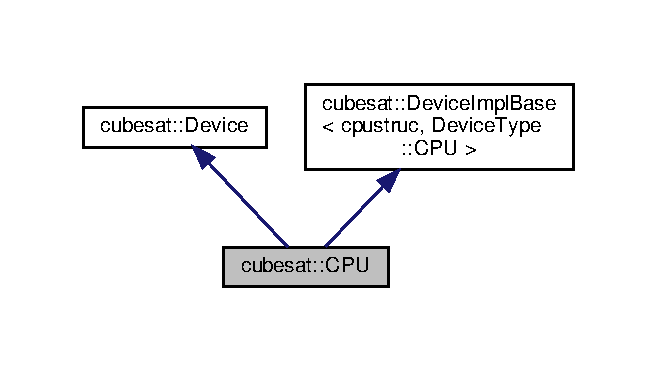
\includegraphics[width=316pt]{classcubesat_1_1CPU__inherit__graph}
\end{center}
\end{figure}


Collaboration diagram for cubesat\+:\+:C\+PU\+:
\nopagebreak
\begin{figure}[H]
\begin{center}
\leavevmode
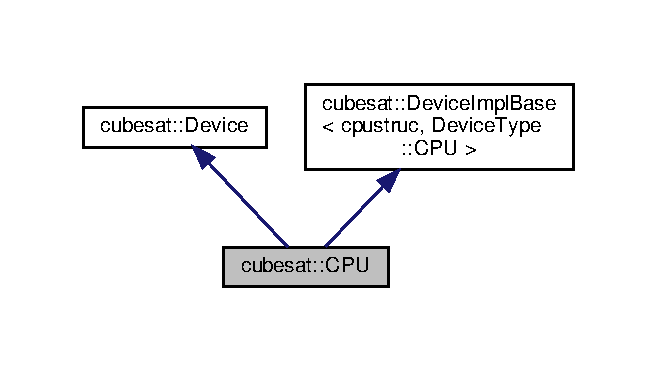
\includegraphics[width=316pt]{classcubesat_1_1CPU__coll__graph}
\end{center}
\end{figure}
\subsection*{Public Member Functions}
\begin{DoxyCompactItemize}
\item 
\hyperlink{classcubesat_1_1CPU_af4d1cfc8a8a5883e651d22c5da12bc23}{C\+PU} (Agent $\ast$\hyperlink{classcubesat_1_1Device_a8499108eccaf7375bea8ead0182391a6}{agent}, int \hyperlink{classcubesat_1_1Device_a1deca725b01f8ef37e49662da6db4e53}{cindex}, int \hyperlink{classcubesat_1_1Device_a8a2b3d6d7400e6796c31705058172982}{dindex})
\item 
virtual \hyperlink{classcubesat_1_1CPU_afb4d0426e2b66c2cee37b77256b9887c}{$\sim$\+C\+PU} ()
\item 
\hyperlink{classcubesat_1_1CPU_a3802b1fceaccca9c8f934c8913bafb45}{\+\_\+\+Add\+Property} (temperature, temp)
\item 
\hyperlink{classcubesat_1_1CPU_ab2bfa609208db1d82154958556295bd7}{\+\_\+\+Add\+Property} (utc, utc)
\item 
\hyperlink{classcubesat_1_1CPU_a3839c4adb3b7deee883e9eebb7dbabad}{\+\_\+\+Add\+Property} (voltage, volt)
\item 
\hyperlink{classcubesat_1_1CPU_a4c9c7a77cf05ac277a6f9f6cb4eb22b2}{\+\_\+\+Add\+Property} (current, amp)
\item 
\hyperlink{classcubesat_1_1CPU_a3663370bc4f9da2a493d3d1d66b892db}{\+\_\+\+Add\+Property} (power, power)
\item 
\hyperlink{classcubesat_1_1CPU_a40d2785d2983d97f9054b320aed84fb6}{\+\_\+\+Add\+Property} (enabled, enabled)
\item 
\hyperlink{classcubesat_1_1CPU_ab0f0b9d475b69dc603ec6242e9a3c074}{\+\_\+\+Add\+Property} (up\+\_\+time, uptime)
\item 
\hyperlink{classcubesat_1_1CPU_a7d1eae11f0dd0f5cffe7eb756ff33187}{\+\_\+\+Add\+Property} (load, load)
\item 
\hyperlink{classcubesat_1_1CPU_a74f8bced81fc233d90e485f1edcbe37b}{\+\_\+\+Add\+Property} (max\+\_\+load, maxload)
\item 
\hyperlink{classcubesat_1_1CPU_afdfc978336cfe4b2390d7f2520041761}{\+\_\+\+Add\+Property} (max\+\_\+memory, maxgib)
\item 
\hyperlink{classcubesat_1_1CPU_a087450dc4ceb02b01420e5a3b894bc95}{\+\_\+\+Add\+Property} (memory\+\_\+usage, gib)
\item 
\hyperlink{classcubesat_1_1CPU_a478fa66d93190e603a0ebfde468a2fb4}{\+\_\+\+Add\+Property} (boot\+\_\+count, boot\+\_\+count)
\end{DoxyCompactItemize}
\subsection*{Additional Inherited Members}


\subsection{Constructor \& Destructor Documentation}
\mbox{\Hypertarget{classcubesat_1_1CPU_af4d1cfc8a8a5883e651d22c5da12bc23}\label{classcubesat_1_1CPU_af4d1cfc8a8a5883e651d22c5da12bc23}} 
\index{cubesat\+::\+C\+PU@{cubesat\+::\+C\+PU}!C\+PU@{C\+PU}}
\index{C\+PU@{C\+PU}!cubesat\+::\+C\+PU@{cubesat\+::\+C\+PU}}
\subsubsection{\texorpdfstring{C\+P\+U()}{CPU()}}
{\footnotesize\ttfamily cubesat\+::\+C\+P\+U\+::\+C\+PU (\begin{DoxyParamCaption}\item[{Agent $\ast$}]{agent,  }\item[{int}]{cindex,  }\item[{int}]{dindex }\end{DoxyParamCaption})\hspace{0.3cm}{\ttfamily [inline]}}

\mbox{\Hypertarget{classcubesat_1_1CPU_afb4d0426e2b66c2cee37b77256b9887c}\label{classcubesat_1_1CPU_afb4d0426e2b66c2cee37b77256b9887c}} 
\index{cubesat\+::\+C\+PU@{cubesat\+::\+C\+PU}!````~C\+PU@{$\sim$\+C\+PU}}
\index{````~C\+PU@{$\sim$\+C\+PU}!cubesat\+::\+C\+PU@{cubesat\+::\+C\+PU}}
\subsubsection{\texorpdfstring{$\sim$\+C\+P\+U()}{~CPU()}}
{\footnotesize\ttfamily virtual cubesat\+::\+C\+P\+U\+::$\sim$\+C\+PU (\begin{DoxyParamCaption}{ }\end{DoxyParamCaption})\hspace{0.3cm}{\ttfamily [inline]}, {\ttfamily [virtual]}}



\subsection{Member Function Documentation}
\mbox{\Hypertarget{classcubesat_1_1CPU_a3802b1fceaccca9c8f934c8913bafb45}\label{classcubesat_1_1CPU_a3802b1fceaccca9c8f934c8913bafb45}} 
\index{cubesat\+::\+C\+PU@{cubesat\+::\+C\+PU}!\+\_\+\+Add\+Property@{\+\_\+\+Add\+Property}}
\index{\+\_\+\+Add\+Property@{\+\_\+\+Add\+Property}!cubesat\+::\+C\+PU@{cubesat\+::\+C\+PU}}
\subsubsection{\texorpdfstring{\+\_\+\+Add\+Property()}{\_AddProperty()}\hspace{0.1cm}{\footnotesize\ttfamily [1/12]}}
{\footnotesize\ttfamily cubesat\+::\+C\+P\+U\+::\+\_\+\+Add\+Property (\begin{DoxyParamCaption}\item[{temperature}]{,  }\item[{temp}]{ }\end{DoxyParamCaption})}

\mbox{\Hypertarget{classcubesat_1_1CPU_ab2bfa609208db1d82154958556295bd7}\label{classcubesat_1_1CPU_ab2bfa609208db1d82154958556295bd7}} 
\index{cubesat\+::\+C\+PU@{cubesat\+::\+C\+PU}!\+\_\+\+Add\+Property@{\+\_\+\+Add\+Property}}
\index{\+\_\+\+Add\+Property@{\+\_\+\+Add\+Property}!cubesat\+::\+C\+PU@{cubesat\+::\+C\+PU}}
\subsubsection{\texorpdfstring{\+\_\+\+Add\+Property()}{\_AddProperty()}\hspace{0.1cm}{\footnotesize\ttfamily [2/12]}}
{\footnotesize\ttfamily cubesat\+::\+C\+P\+U\+::\+\_\+\+Add\+Property (\begin{DoxyParamCaption}\item[{utc}]{,  }\item[{utc}]{ }\end{DoxyParamCaption})}

\mbox{\Hypertarget{classcubesat_1_1CPU_a3839c4adb3b7deee883e9eebb7dbabad}\label{classcubesat_1_1CPU_a3839c4adb3b7deee883e9eebb7dbabad}} 
\index{cubesat\+::\+C\+PU@{cubesat\+::\+C\+PU}!\+\_\+\+Add\+Property@{\+\_\+\+Add\+Property}}
\index{\+\_\+\+Add\+Property@{\+\_\+\+Add\+Property}!cubesat\+::\+C\+PU@{cubesat\+::\+C\+PU}}
\subsubsection{\texorpdfstring{\+\_\+\+Add\+Property()}{\_AddProperty()}\hspace{0.1cm}{\footnotesize\ttfamily [3/12]}}
{\footnotesize\ttfamily cubesat\+::\+C\+P\+U\+::\+\_\+\+Add\+Property (\begin{DoxyParamCaption}\item[{voltage}]{,  }\item[{volt}]{ }\end{DoxyParamCaption})}

\mbox{\Hypertarget{classcubesat_1_1CPU_a4c9c7a77cf05ac277a6f9f6cb4eb22b2}\label{classcubesat_1_1CPU_a4c9c7a77cf05ac277a6f9f6cb4eb22b2}} 
\index{cubesat\+::\+C\+PU@{cubesat\+::\+C\+PU}!\+\_\+\+Add\+Property@{\+\_\+\+Add\+Property}}
\index{\+\_\+\+Add\+Property@{\+\_\+\+Add\+Property}!cubesat\+::\+C\+PU@{cubesat\+::\+C\+PU}}
\subsubsection{\texorpdfstring{\+\_\+\+Add\+Property()}{\_AddProperty()}\hspace{0.1cm}{\footnotesize\ttfamily [4/12]}}
{\footnotesize\ttfamily cubesat\+::\+C\+P\+U\+::\+\_\+\+Add\+Property (\begin{DoxyParamCaption}\item[{current}]{,  }\item[{amp}]{ }\end{DoxyParamCaption})}

\mbox{\Hypertarget{classcubesat_1_1CPU_a3663370bc4f9da2a493d3d1d66b892db}\label{classcubesat_1_1CPU_a3663370bc4f9da2a493d3d1d66b892db}} 
\index{cubesat\+::\+C\+PU@{cubesat\+::\+C\+PU}!\+\_\+\+Add\+Property@{\+\_\+\+Add\+Property}}
\index{\+\_\+\+Add\+Property@{\+\_\+\+Add\+Property}!cubesat\+::\+C\+PU@{cubesat\+::\+C\+PU}}
\subsubsection{\texorpdfstring{\+\_\+\+Add\+Property()}{\_AddProperty()}\hspace{0.1cm}{\footnotesize\ttfamily [5/12]}}
{\footnotesize\ttfamily cubesat\+::\+C\+P\+U\+::\+\_\+\+Add\+Property (\begin{DoxyParamCaption}\item[{power}]{,  }\item[{power}]{ }\end{DoxyParamCaption})}

\mbox{\Hypertarget{classcubesat_1_1CPU_a40d2785d2983d97f9054b320aed84fb6}\label{classcubesat_1_1CPU_a40d2785d2983d97f9054b320aed84fb6}} 
\index{cubesat\+::\+C\+PU@{cubesat\+::\+C\+PU}!\+\_\+\+Add\+Property@{\+\_\+\+Add\+Property}}
\index{\+\_\+\+Add\+Property@{\+\_\+\+Add\+Property}!cubesat\+::\+C\+PU@{cubesat\+::\+C\+PU}}
\subsubsection{\texorpdfstring{\+\_\+\+Add\+Property()}{\_AddProperty()}\hspace{0.1cm}{\footnotesize\ttfamily [6/12]}}
{\footnotesize\ttfamily cubesat\+::\+C\+P\+U\+::\+\_\+\+Add\+Property (\begin{DoxyParamCaption}\item[{enabled}]{,  }\item[{enabled}]{ }\end{DoxyParamCaption})}

\mbox{\Hypertarget{classcubesat_1_1CPU_ab0f0b9d475b69dc603ec6242e9a3c074}\label{classcubesat_1_1CPU_ab0f0b9d475b69dc603ec6242e9a3c074}} 
\index{cubesat\+::\+C\+PU@{cubesat\+::\+C\+PU}!\+\_\+\+Add\+Property@{\+\_\+\+Add\+Property}}
\index{\+\_\+\+Add\+Property@{\+\_\+\+Add\+Property}!cubesat\+::\+C\+PU@{cubesat\+::\+C\+PU}}
\subsubsection{\texorpdfstring{\+\_\+\+Add\+Property()}{\_AddProperty()}\hspace{0.1cm}{\footnotesize\ttfamily [7/12]}}
{\footnotesize\ttfamily cubesat\+::\+C\+P\+U\+::\+\_\+\+Add\+Property (\begin{DoxyParamCaption}\item[{up\+\_\+time}]{,  }\item[{uptime}]{ }\end{DoxyParamCaption})}

\mbox{\Hypertarget{classcubesat_1_1CPU_a7d1eae11f0dd0f5cffe7eb756ff33187}\label{classcubesat_1_1CPU_a7d1eae11f0dd0f5cffe7eb756ff33187}} 
\index{cubesat\+::\+C\+PU@{cubesat\+::\+C\+PU}!\+\_\+\+Add\+Property@{\+\_\+\+Add\+Property}}
\index{\+\_\+\+Add\+Property@{\+\_\+\+Add\+Property}!cubesat\+::\+C\+PU@{cubesat\+::\+C\+PU}}
\subsubsection{\texorpdfstring{\+\_\+\+Add\+Property()}{\_AddProperty()}\hspace{0.1cm}{\footnotesize\ttfamily [8/12]}}
{\footnotesize\ttfamily cubesat\+::\+C\+P\+U\+::\+\_\+\+Add\+Property (\begin{DoxyParamCaption}\item[{load}]{,  }\item[{load}]{ }\end{DoxyParamCaption})}

\mbox{\Hypertarget{classcubesat_1_1CPU_a74f8bced81fc233d90e485f1edcbe37b}\label{classcubesat_1_1CPU_a74f8bced81fc233d90e485f1edcbe37b}} 
\index{cubesat\+::\+C\+PU@{cubesat\+::\+C\+PU}!\+\_\+\+Add\+Property@{\+\_\+\+Add\+Property}}
\index{\+\_\+\+Add\+Property@{\+\_\+\+Add\+Property}!cubesat\+::\+C\+PU@{cubesat\+::\+C\+PU}}
\subsubsection{\texorpdfstring{\+\_\+\+Add\+Property()}{\_AddProperty()}\hspace{0.1cm}{\footnotesize\ttfamily [9/12]}}
{\footnotesize\ttfamily cubesat\+::\+C\+P\+U\+::\+\_\+\+Add\+Property (\begin{DoxyParamCaption}\item[{max\+\_\+load}]{,  }\item[{maxload}]{ }\end{DoxyParamCaption})}

\mbox{\Hypertarget{classcubesat_1_1CPU_afdfc978336cfe4b2390d7f2520041761}\label{classcubesat_1_1CPU_afdfc978336cfe4b2390d7f2520041761}} 
\index{cubesat\+::\+C\+PU@{cubesat\+::\+C\+PU}!\+\_\+\+Add\+Property@{\+\_\+\+Add\+Property}}
\index{\+\_\+\+Add\+Property@{\+\_\+\+Add\+Property}!cubesat\+::\+C\+PU@{cubesat\+::\+C\+PU}}
\subsubsection{\texorpdfstring{\+\_\+\+Add\+Property()}{\_AddProperty()}\hspace{0.1cm}{\footnotesize\ttfamily [10/12]}}
{\footnotesize\ttfamily cubesat\+::\+C\+P\+U\+::\+\_\+\+Add\+Property (\begin{DoxyParamCaption}\item[{max\+\_\+memory}]{,  }\item[{maxgib}]{ }\end{DoxyParamCaption})}

\mbox{\Hypertarget{classcubesat_1_1CPU_a087450dc4ceb02b01420e5a3b894bc95}\label{classcubesat_1_1CPU_a087450dc4ceb02b01420e5a3b894bc95}} 
\index{cubesat\+::\+C\+PU@{cubesat\+::\+C\+PU}!\+\_\+\+Add\+Property@{\+\_\+\+Add\+Property}}
\index{\+\_\+\+Add\+Property@{\+\_\+\+Add\+Property}!cubesat\+::\+C\+PU@{cubesat\+::\+C\+PU}}
\subsubsection{\texorpdfstring{\+\_\+\+Add\+Property()}{\_AddProperty()}\hspace{0.1cm}{\footnotesize\ttfamily [11/12]}}
{\footnotesize\ttfamily cubesat\+::\+C\+P\+U\+::\+\_\+\+Add\+Property (\begin{DoxyParamCaption}\item[{memory\+\_\+usage}]{,  }\item[{gib}]{ }\end{DoxyParamCaption})}

\mbox{\Hypertarget{classcubesat_1_1CPU_a478fa66d93190e603a0ebfde468a2fb4}\label{classcubesat_1_1CPU_a478fa66d93190e603a0ebfde468a2fb4}} 
\index{cubesat\+::\+C\+PU@{cubesat\+::\+C\+PU}!\+\_\+\+Add\+Property@{\+\_\+\+Add\+Property}}
\index{\+\_\+\+Add\+Property@{\+\_\+\+Add\+Property}!cubesat\+::\+C\+PU@{cubesat\+::\+C\+PU}}
\subsubsection{\texorpdfstring{\+\_\+\+Add\+Property()}{\_AddProperty()}\hspace{0.1cm}{\footnotesize\ttfamily [12/12]}}
{\footnotesize\ttfamily cubesat\+::\+C\+P\+U\+::\+\_\+\+Add\+Property (\begin{DoxyParamCaption}\item[{boot\+\_\+count}]{,  }\item[{boot\+\_\+count}]{ }\end{DoxyParamCaption})}



The documentation for this class was generated from the following file\+:\begin{DoxyCompactItemize}
\item 
/home/osboxes/cosmos/source/projects/cubesat-\/kit/include/utility/\hyperlink{Device_8h}{Device.\+h}\end{DoxyCompactItemize}

\hypertarget{classcubesat_1_1CustomDevice}{}\section{cubesat\+:\+:Custom\+Device Class Reference}
\label{classcubesat_1_1CustomDevice}\index{cubesat\+::\+Custom\+Device@{cubesat\+::\+Custom\+Device}}


{\ttfamily \#include $<$Device.\+h$>$}



Inheritance diagram for cubesat\+:\+:Custom\+Device\+:
\nopagebreak
\begin{figure}[H]
\begin{center}
\leavevmode
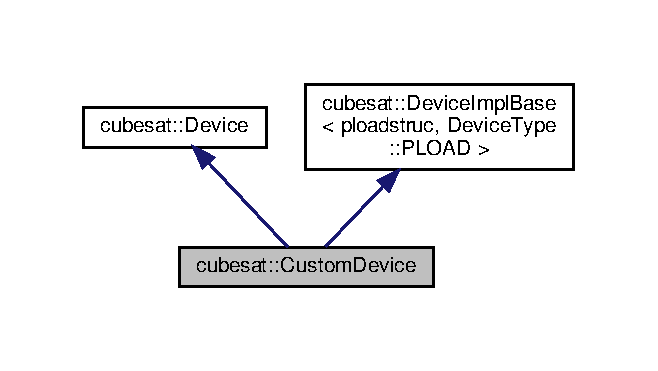
\includegraphics[width=316pt]{classcubesat_1_1CustomDevice__inherit__graph}
\end{center}
\end{figure}


Collaboration diagram for cubesat\+:\+:Custom\+Device\+:
\nopagebreak
\begin{figure}[H]
\begin{center}
\leavevmode
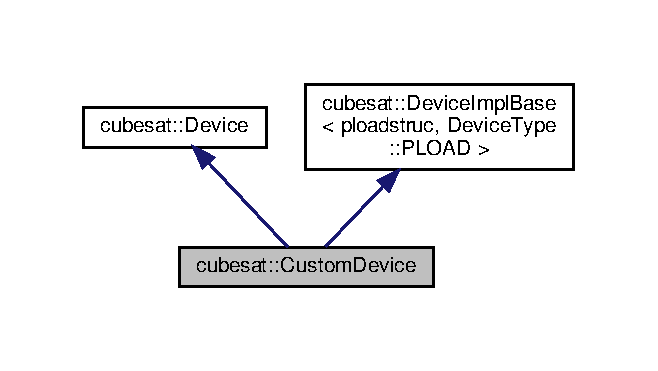
\includegraphics[width=316pt]{classcubesat_1_1CustomDevice__coll__graph}
\end{center}
\end{figure}
\subsection*{Public Member Functions}
\begin{DoxyCompactItemize}
\item 
\hyperlink{classcubesat_1_1CustomDevice_a4f4beb9537b183cfad81ce08ebaea622}{Custom\+Device} (Agent $\ast$\hyperlink{classcubesat_1_1Device_a8499108eccaf7375bea8ead0182391a6}{agent}, int \hyperlink{classcubesat_1_1Device_a1deca725b01f8ef37e49662da6db4e53}{cindex}, int \hyperlink{classcubesat_1_1Device_a8a2b3d6d7400e6796c31705058172982}{dindex})
\item 
virtual \hyperlink{classcubesat_1_1CustomDevice_afd2d3db110cc3c67a635f2cdf76db81e}{$\sim$\+Custom\+Device} ()
\item 
\hyperlink{classcubesat_1_1CustomDevice_a2db96c92e03c4f4217e0217764fd4147}{\+\_\+\+Add\+Property} (temperature, temp)
\item 
\hyperlink{classcubesat_1_1CustomDevice_a44680935c5a224147a965fe97289d13c}{\+\_\+\+Add\+Property} (utc, utc)
\item 
\hyperlink{classcubesat_1_1CustomDevice_a3a15eff13cba7ca61bb845fdc2e26655}{\+\_\+\+Add\+Property} (voltage, volt)
\item 
\hyperlink{classcubesat_1_1CustomDevice_a99fcae6764531a5e3b8a7e5957704461}{\+\_\+\+Add\+Property} (current, amp)
\item 
\hyperlink{classcubesat_1_1CustomDevice_a08d07a6fd08acc7064301ea4d9f927a3}{\+\_\+\+Add\+Property} (power, power)
\item 
\hyperlink{classcubesat_1_1CustomDevice_adde28cab76c394ba807623d328bca1b1}{\+\_\+\+Add\+Property} (enabled, enabled)
\end{DoxyCompactItemize}
\subsection*{Additional Inherited Members}


\subsection{Constructor \& Destructor Documentation}
\mbox{\Hypertarget{classcubesat_1_1CustomDevice_a4f4beb9537b183cfad81ce08ebaea622}\label{classcubesat_1_1CustomDevice_a4f4beb9537b183cfad81ce08ebaea622}} 
\index{cubesat\+::\+Custom\+Device@{cubesat\+::\+Custom\+Device}!Custom\+Device@{Custom\+Device}}
\index{Custom\+Device@{Custom\+Device}!cubesat\+::\+Custom\+Device@{cubesat\+::\+Custom\+Device}}
\subsubsection{\texorpdfstring{Custom\+Device()}{CustomDevice()}}
{\footnotesize\ttfamily cubesat\+::\+Custom\+Device\+::\+Custom\+Device (\begin{DoxyParamCaption}\item[{Agent $\ast$}]{agent,  }\item[{int}]{cindex,  }\item[{int}]{dindex }\end{DoxyParamCaption})\hspace{0.3cm}{\ttfamily [inline]}}

\mbox{\Hypertarget{classcubesat_1_1CustomDevice_afd2d3db110cc3c67a635f2cdf76db81e}\label{classcubesat_1_1CustomDevice_afd2d3db110cc3c67a635f2cdf76db81e}} 
\index{cubesat\+::\+Custom\+Device@{cubesat\+::\+Custom\+Device}!````~Custom\+Device@{$\sim$\+Custom\+Device}}
\index{````~Custom\+Device@{$\sim$\+Custom\+Device}!cubesat\+::\+Custom\+Device@{cubesat\+::\+Custom\+Device}}
\subsubsection{\texorpdfstring{$\sim$\+Custom\+Device()}{~CustomDevice()}}
{\footnotesize\ttfamily virtual cubesat\+::\+Custom\+Device\+::$\sim$\+Custom\+Device (\begin{DoxyParamCaption}{ }\end{DoxyParamCaption})\hspace{0.3cm}{\ttfamily [inline]}, {\ttfamily [virtual]}}



\subsection{Member Function Documentation}
\mbox{\Hypertarget{classcubesat_1_1CustomDevice_a2db96c92e03c4f4217e0217764fd4147}\label{classcubesat_1_1CustomDevice_a2db96c92e03c4f4217e0217764fd4147}} 
\index{cubesat\+::\+Custom\+Device@{cubesat\+::\+Custom\+Device}!\+\_\+\+Add\+Property@{\+\_\+\+Add\+Property}}
\index{\+\_\+\+Add\+Property@{\+\_\+\+Add\+Property}!cubesat\+::\+Custom\+Device@{cubesat\+::\+Custom\+Device}}
\subsubsection{\texorpdfstring{\+\_\+\+Add\+Property()}{\_AddProperty()}\hspace{0.1cm}{\footnotesize\ttfamily [1/6]}}
{\footnotesize\ttfamily cubesat\+::\+Custom\+Device\+::\+\_\+\+Add\+Property (\begin{DoxyParamCaption}\item[{temperature}]{,  }\item[{temp}]{ }\end{DoxyParamCaption})}

\mbox{\Hypertarget{classcubesat_1_1CustomDevice_a44680935c5a224147a965fe97289d13c}\label{classcubesat_1_1CustomDevice_a44680935c5a224147a965fe97289d13c}} 
\index{cubesat\+::\+Custom\+Device@{cubesat\+::\+Custom\+Device}!\+\_\+\+Add\+Property@{\+\_\+\+Add\+Property}}
\index{\+\_\+\+Add\+Property@{\+\_\+\+Add\+Property}!cubesat\+::\+Custom\+Device@{cubesat\+::\+Custom\+Device}}
\subsubsection{\texorpdfstring{\+\_\+\+Add\+Property()}{\_AddProperty()}\hspace{0.1cm}{\footnotesize\ttfamily [2/6]}}
{\footnotesize\ttfamily cubesat\+::\+Custom\+Device\+::\+\_\+\+Add\+Property (\begin{DoxyParamCaption}\item[{utc}]{,  }\item[{utc}]{ }\end{DoxyParamCaption})}

\mbox{\Hypertarget{classcubesat_1_1CustomDevice_a3a15eff13cba7ca61bb845fdc2e26655}\label{classcubesat_1_1CustomDevice_a3a15eff13cba7ca61bb845fdc2e26655}} 
\index{cubesat\+::\+Custom\+Device@{cubesat\+::\+Custom\+Device}!\+\_\+\+Add\+Property@{\+\_\+\+Add\+Property}}
\index{\+\_\+\+Add\+Property@{\+\_\+\+Add\+Property}!cubesat\+::\+Custom\+Device@{cubesat\+::\+Custom\+Device}}
\subsubsection{\texorpdfstring{\+\_\+\+Add\+Property()}{\_AddProperty()}\hspace{0.1cm}{\footnotesize\ttfamily [3/6]}}
{\footnotesize\ttfamily cubesat\+::\+Custom\+Device\+::\+\_\+\+Add\+Property (\begin{DoxyParamCaption}\item[{voltage}]{,  }\item[{volt}]{ }\end{DoxyParamCaption})}

\mbox{\Hypertarget{classcubesat_1_1CustomDevice_a99fcae6764531a5e3b8a7e5957704461}\label{classcubesat_1_1CustomDevice_a99fcae6764531a5e3b8a7e5957704461}} 
\index{cubesat\+::\+Custom\+Device@{cubesat\+::\+Custom\+Device}!\+\_\+\+Add\+Property@{\+\_\+\+Add\+Property}}
\index{\+\_\+\+Add\+Property@{\+\_\+\+Add\+Property}!cubesat\+::\+Custom\+Device@{cubesat\+::\+Custom\+Device}}
\subsubsection{\texorpdfstring{\+\_\+\+Add\+Property()}{\_AddProperty()}\hspace{0.1cm}{\footnotesize\ttfamily [4/6]}}
{\footnotesize\ttfamily cubesat\+::\+Custom\+Device\+::\+\_\+\+Add\+Property (\begin{DoxyParamCaption}\item[{current}]{,  }\item[{amp}]{ }\end{DoxyParamCaption})}

\mbox{\Hypertarget{classcubesat_1_1CustomDevice_a08d07a6fd08acc7064301ea4d9f927a3}\label{classcubesat_1_1CustomDevice_a08d07a6fd08acc7064301ea4d9f927a3}} 
\index{cubesat\+::\+Custom\+Device@{cubesat\+::\+Custom\+Device}!\+\_\+\+Add\+Property@{\+\_\+\+Add\+Property}}
\index{\+\_\+\+Add\+Property@{\+\_\+\+Add\+Property}!cubesat\+::\+Custom\+Device@{cubesat\+::\+Custom\+Device}}
\subsubsection{\texorpdfstring{\+\_\+\+Add\+Property()}{\_AddProperty()}\hspace{0.1cm}{\footnotesize\ttfamily [5/6]}}
{\footnotesize\ttfamily cubesat\+::\+Custom\+Device\+::\+\_\+\+Add\+Property (\begin{DoxyParamCaption}\item[{power}]{,  }\item[{power}]{ }\end{DoxyParamCaption})}

\mbox{\Hypertarget{classcubesat_1_1CustomDevice_adde28cab76c394ba807623d328bca1b1}\label{classcubesat_1_1CustomDevice_adde28cab76c394ba807623d328bca1b1}} 
\index{cubesat\+::\+Custom\+Device@{cubesat\+::\+Custom\+Device}!\+\_\+\+Add\+Property@{\+\_\+\+Add\+Property}}
\index{\+\_\+\+Add\+Property@{\+\_\+\+Add\+Property}!cubesat\+::\+Custom\+Device@{cubesat\+::\+Custom\+Device}}
\subsubsection{\texorpdfstring{\+\_\+\+Add\+Property()}{\_AddProperty()}\hspace{0.1cm}{\footnotesize\ttfamily [6/6]}}
{\footnotesize\ttfamily cubesat\+::\+Custom\+Device\+::\+\_\+\+Add\+Property (\begin{DoxyParamCaption}\item[{enabled}]{,  }\item[{enabled}]{ }\end{DoxyParamCaption})}



The documentation for this class was generated from the following file\+:\begin{DoxyCompactItemize}
\item 
/home/osboxes/cosmos/source/projects/cubesat-\/kit/include/utility/\hyperlink{Device_8h}{Device.\+h}\end{DoxyCompactItemize}

\hypertarget{structcubesat_1_1Device_1_1CustomProperty}{}\section{cubesat\+:\+:Device\+:\+:Custom\+Property Struct Reference}
\label{structcubesat_1_1Device_1_1CustomProperty}\index{cubesat\+::\+Device\+::\+Custom\+Property@{cubesat\+::\+Device\+::\+Custom\+Property}}
\subsection*{Public Member Functions}
\begin{DoxyCompactItemize}
\item 
\hyperlink{structcubesat_1_1Device_1_1CustomProperty_a25a532733331b17d7320ea491f0a5d9d}{Custom\+Property} ()
\item 
\hyperlink{structcubesat_1_1Device_1_1CustomProperty_a2e47a4d6fa0897143547282a9917d6f6}{Custom\+Property} (const \hyperlink{structcubesat_1_1Device_1_1CustomProperty}{Custom\+Property} \&other)=delete
\item 
\hyperlink{structcubesat_1_1Device_1_1CustomProperty_a95fbf77d154d897d33e629c5734ca299}{$\sim$\+Custom\+Property} ()
\item 
{\footnotesize template$<$typename T $>$ }\\bool \hyperlink{structcubesat_1_1Device_1_1CustomProperty_a1de276a5b24206e3bbcd6417dd9ef513}{Type\+Matches} ()
\item 
{\footnotesize template$<$typename T $>$ }\\void \hyperlink{structcubesat_1_1Device_1_1CustomProperty_abba6f25cccf279e9e69820978546abf9}{Load} (T value\+\_\+)
\item 
{\footnotesize template$<$typename T $>$ }\\void \hyperlink{structcubesat_1_1Device_1_1CustomProperty_a4cd2124bf2c57ea23c2b8b217377422c}{Set} (T value\+\_\+)
\end{DoxyCompactItemize}
\subsection*{Public Attributes}
\begin{DoxyCompactItemize}
\item 
void $\ast$ \hyperlink{structcubesat_1_1Device_1_1CustomProperty_a6e11ec1c5cfdd9c392f60260eecb6698}{value}
\item 
\hyperlink{namespacecubesat_ab5c769503b8a77bc90a47ca8705f2f86}{Property\+ID} \hyperlink{structcubesat_1_1Device_1_1CustomProperty_ac9cd21a36cd666169540dc5acda390b3}{value\+\_\+type}
\end{DoxyCompactItemize}


\subsection{Constructor \& Destructor Documentation}
\mbox{\Hypertarget{structcubesat_1_1Device_1_1CustomProperty_a25a532733331b17d7320ea491f0a5d9d}\label{structcubesat_1_1Device_1_1CustomProperty_a25a532733331b17d7320ea491f0a5d9d}} 
\index{cubesat\+::\+Device\+::\+Custom\+Property@{cubesat\+::\+Device\+::\+Custom\+Property}!Custom\+Property@{Custom\+Property}}
\index{Custom\+Property@{Custom\+Property}!cubesat\+::\+Device\+::\+Custom\+Property@{cubesat\+::\+Device\+::\+Custom\+Property}}
\subsubsection{\texorpdfstring{Custom\+Property()}{CustomProperty()}\hspace{0.1cm}{\footnotesize\ttfamily [1/2]}}
{\footnotesize\ttfamily cubesat\+::\+Device\+::\+Custom\+Property\+::\+Custom\+Property (\begin{DoxyParamCaption}{ }\end{DoxyParamCaption})\hspace{0.3cm}{\ttfamily [inline]}}

\mbox{\Hypertarget{structcubesat_1_1Device_1_1CustomProperty_a2e47a4d6fa0897143547282a9917d6f6}\label{structcubesat_1_1Device_1_1CustomProperty_a2e47a4d6fa0897143547282a9917d6f6}} 
\index{cubesat\+::\+Device\+::\+Custom\+Property@{cubesat\+::\+Device\+::\+Custom\+Property}!Custom\+Property@{Custom\+Property}}
\index{Custom\+Property@{Custom\+Property}!cubesat\+::\+Device\+::\+Custom\+Property@{cubesat\+::\+Device\+::\+Custom\+Property}}
\subsubsection{\texorpdfstring{Custom\+Property()}{CustomProperty()}\hspace{0.1cm}{\footnotesize\ttfamily [2/2]}}
{\footnotesize\ttfamily cubesat\+::\+Device\+::\+Custom\+Property\+::\+Custom\+Property (\begin{DoxyParamCaption}\item[{const \hyperlink{structcubesat_1_1Device_1_1CustomProperty}{Custom\+Property} \&}]{other }\end{DoxyParamCaption})\hspace{0.3cm}{\ttfamily [delete]}}

\mbox{\Hypertarget{structcubesat_1_1Device_1_1CustomProperty_a95fbf77d154d897d33e629c5734ca299}\label{structcubesat_1_1Device_1_1CustomProperty_a95fbf77d154d897d33e629c5734ca299}} 
\index{cubesat\+::\+Device\+::\+Custom\+Property@{cubesat\+::\+Device\+::\+Custom\+Property}!````~Custom\+Property@{$\sim$\+Custom\+Property}}
\index{````~Custom\+Property@{$\sim$\+Custom\+Property}!cubesat\+::\+Device\+::\+Custom\+Property@{cubesat\+::\+Device\+::\+Custom\+Property}}
\subsubsection{\texorpdfstring{$\sim$\+Custom\+Property()}{~CustomProperty()}}
{\footnotesize\ttfamily cubesat\+::\+Device\+::\+Custom\+Property\+::$\sim$\+Custom\+Property (\begin{DoxyParamCaption}{ }\end{DoxyParamCaption})\hspace{0.3cm}{\ttfamily [inline]}}



\subsection{Member Function Documentation}
\mbox{\Hypertarget{structcubesat_1_1Device_1_1CustomProperty_abba6f25cccf279e9e69820978546abf9}\label{structcubesat_1_1Device_1_1CustomProperty_abba6f25cccf279e9e69820978546abf9}} 
\index{cubesat\+::\+Device\+::\+Custom\+Property@{cubesat\+::\+Device\+::\+Custom\+Property}!Load@{Load}}
\index{Load@{Load}!cubesat\+::\+Device\+::\+Custom\+Property@{cubesat\+::\+Device\+::\+Custom\+Property}}
\subsubsection{\texorpdfstring{Load()}{Load()}}
{\footnotesize\ttfamily template$<$typename T $>$ \\
void cubesat\+::\+Device\+::\+Custom\+Property\+::\+Load (\begin{DoxyParamCaption}\item[{T}]{value\+\_\+ }\end{DoxyParamCaption})\hspace{0.3cm}{\ttfamily [inline]}}

\mbox{\Hypertarget{structcubesat_1_1Device_1_1CustomProperty_a4cd2124bf2c57ea23c2b8b217377422c}\label{structcubesat_1_1Device_1_1CustomProperty_a4cd2124bf2c57ea23c2b8b217377422c}} 
\index{cubesat\+::\+Device\+::\+Custom\+Property@{cubesat\+::\+Device\+::\+Custom\+Property}!Set@{Set}}
\index{Set@{Set}!cubesat\+::\+Device\+::\+Custom\+Property@{cubesat\+::\+Device\+::\+Custom\+Property}}
\subsubsection{\texorpdfstring{Set()}{Set()}}
{\footnotesize\ttfamily template$<$typename T $>$ \\
void cubesat\+::\+Device\+::\+Custom\+Property\+::\+Set (\begin{DoxyParamCaption}\item[{T}]{value\+\_\+ }\end{DoxyParamCaption})\hspace{0.3cm}{\ttfamily [inline]}}

\mbox{\Hypertarget{structcubesat_1_1Device_1_1CustomProperty_a1de276a5b24206e3bbcd6417dd9ef513}\label{structcubesat_1_1Device_1_1CustomProperty_a1de276a5b24206e3bbcd6417dd9ef513}} 
\index{cubesat\+::\+Device\+::\+Custom\+Property@{cubesat\+::\+Device\+::\+Custom\+Property}!Type\+Matches@{Type\+Matches}}
\index{Type\+Matches@{Type\+Matches}!cubesat\+::\+Device\+::\+Custom\+Property@{cubesat\+::\+Device\+::\+Custom\+Property}}
\subsubsection{\texorpdfstring{Type\+Matches()}{TypeMatches()}}
{\footnotesize\ttfamily template$<$typename T $>$ \\
bool cubesat\+::\+Device\+::\+Custom\+Property\+::\+Type\+Matches (\begin{DoxyParamCaption}{ }\end{DoxyParamCaption})\hspace{0.3cm}{\ttfamily [inline]}}



\subsection{Member Data Documentation}
\mbox{\Hypertarget{structcubesat_1_1Device_1_1CustomProperty_a6e11ec1c5cfdd9c392f60260eecb6698}\label{structcubesat_1_1Device_1_1CustomProperty_a6e11ec1c5cfdd9c392f60260eecb6698}} 
\index{cubesat\+::\+Device\+::\+Custom\+Property@{cubesat\+::\+Device\+::\+Custom\+Property}!value@{value}}
\index{value@{value}!cubesat\+::\+Device\+::\+Custom\+Property@{cubesat\+::\+Device\+::\+Custom\+Property}}
\subsubsection{\texorpdfstring{value}{value}}
{\footnotesize\ttfamily void$\ast$ cubesat\+::\+Device\+::\+Custom\+Property\+::value}

\mbox{\Hypertarget{structcubesat_1_1Device_1_1CustomProperty_ac9cd21a36cd666169540dc5acda390b3}\label{structcubesat_1_1Device_1_1CustomProperty_ac9cd21a36cd666169540dc5acda390b3}} 
\index{cubesat\+::\+Device\+::\+Custom\+Property@{cubesat\+::\+Device\+::\+Custom\+Property}!value\+\_\+type@{value\+\_\+type}}
\index{value\+\_\+type@{value\+\_\+type}!cubesat\+::\+Device\+::\+Custom\+Property@{cubesat\+::\+Device\+::\+Custom\+Property}}
\subsubsection{\texorpdfstring{value\+\_\+type}{value\_type}}
{\footnotesize\ttfamily \hyperlink{namespacecubesat_ab5c769503b8a77bc90a47ca8705f2f86}{Property\+ID} cubesat\+::\+Device\+::\+Custom\+Property\+::value\+\_\+type}



The documentation for this struct was generated from the following file\+:\begin{DoxyCompactItemize}
\item 
/home/osboxes/cosmos/source/projects/cubesat-\/kit/include/utility/\hyperlink{Device_8h}{Device.\+h}\end{DoxyCompactItemize}

\hypertarget{classcubesat_1_1Device}{}\section{cubesat\+:\+:Device Class Reference}
\label{classcubesat_1_1Device}\index{cubesat\+::\+Device@{cubesat\+::\+Device}}


Holds information about a device, and allows for properties to be posted in an agent\textquotesingle{}s state of health message.  




{\ttfamily \#include $<$Device.\+h$>$}



Inheritance diagram for cubesat\+:\+:Device\+:
\nopagebreak
\begin{figure}[H]
\begin{center}
\leavevmode
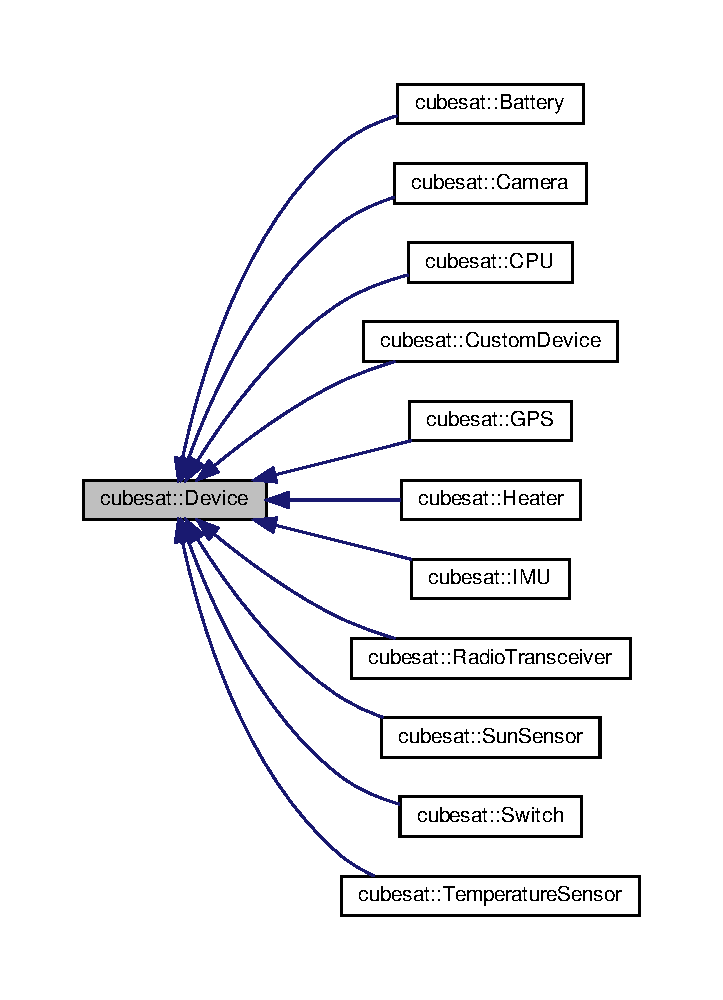
\includegraphics[width=347pt]{classcubesat_1_1Device__inherit__graph}
\end{center}
\end{figure}
\subsection*{Classes}
\begin{DoxyCompactItemize}
\item 
struct \hyperlink{structcubesat_1_1Device_1_1CustomProperty}{Custom\+Property}
\item 
struct \hyperlink{structcubesat_1_1Device_1_1PostedProperty}{Posted\+Property}
\end{DoxyCompactItemize}
\subsection*{Public Member Functions}
\begin{DoxyCompactItemize}
\item 
\hyperlink{classcubesat_1_1Device_a19869b78d586dff676fa6ef25ccaa779}{Device} (Agent $\ast$\hyperlink{classcubesat_1_1Device_a8499108eccaf7375bea8ead0182391a6}{agent}, int \hyperlink{classcubesat_1_1Device_a1deca725b01f8ef37e49662da6db4e53}{cindex}, int \hyperlink{classcubesat_1_1Device_a8a2b3d6d7400e6796c31705058172982}{dindex}, const std\+::string \&\hyperlink{classcubesat_1_1Device_a90904a89fe9cf559e50028a7d0cb878f}{cosmos\+\_\+device\+\_\+name})
\begin{DoxyCompactList}\small\item\em Creates a new device. \end{DoxyCompactList}\item 
virtual \hyperlink{classcubesat_1_1Device_a60a17b504ad734b977d4d87b2f0151f0}{$\sim$\+Device} ()
\item 
{\footnotesize template$<$typename \+\_\+\+Property\+Type $>$ }\\void \hyperlink{classcubesat_1_1Device_a307f4f199eb01b10e44e3b6a42034349}{Post} (const \+\_\+\+Property\+Type \&property)
\begin{DoxyCompactList}\small\item\em Posts a property to the state of health message. \end{DoxyCompactList}\item 
void \hyperlink{classcubesat_1_1Device_ae273ac30edc470b3623853d74fd22e90}{Store\+Posted\+Properties} (std\+::vector$<$ std\+::string $>$ \&keys)
\begin{DoxyCompactList}\small\item\em Adds all posted properties to the given vector. \end{DoxyCompactList}\item 
bool \hyperlink{classcubesat_1_1Device_a7174eacedcecf65bbf2d7ad0f28d10e1}{Custom\+Property\+Exists} (const std\+::string \&name)
\begin{DoxyCompactList}\small\item\em Checks if a custom property with the given name exists. \end{DoxyCompactList}\item 
{\footnotesize template$<$typename T $>$ }\\void \hyperlink{classcubesat_1_1Device_a586d450c984461a04503e895758cafcb}{Set\+Custom\+Property} (const std\+::string \&name, T value)
\begin{DoxyCompactList}\small\item\em Stores a custom property. \end{DoxyCompactList}\item 
{\footnotesize template$<$typename T $>$ }\\T \& \hyperlink{classcubesat_1_1Device_abdd7840e18fc3fe8127641819817450d}{Get\+Custom\+Property} (const std\+::string \&name)
\begin{DoxyCompactList}\small\item\em Retrieves a custom property from this device. \end{DoxyCompactList}\item 
void \hyperlink{classcubesat_1_1Device_ac93bdbe5c92221c158dfc58b60518956}{Debug\+Print} ()
\begin{DoxyCompactList}\small\item\em Prints information about this device. \end{DoxyCompactList}\item 
void \hyperlink{classcubesat_1_1Device_a2bc1682e91b0e2cce693bd7f2f88f052}{Get\+Debug\+String} (std\+::stringstream \&ss)
\begin{DoxyCompactList}\small\item\em Prints information about this device to an std\+:stringstream. \end{DoxyCompactList}\item 
void \hyperlink{classcubesat_1_1Device_a90374e827bf35d0ec47d5983b55a892b}{Set\+Name} (const std\+::string \&\hyperlink{classcubesat_1_1Device_abb55814f123cad387d84a0802da29bd7}{device\+\_\+name})
\item 
const std\+::string \& \hyperlink{classcubesat_1_1Device_a599328b0664f0ea2099e3ca1de79779f}{Get\+Name} () const
\end{DoxyCompactItemize}
\subsection*{Protected Member Functions}
\begin{DoxyCompactItemize}
\item 
std\+::string \hyperlink{classcubesat_1_1Device_ad658ff2e014f927a65673a15e15ae4ba}{Get\+C\+O\+S\+M\+O\+S\+Property\+Name} (const std\+::string \&cosmos\+\_\+property\+\_\+name)
\end{DoxyCompactItemize}
\subsection*{Protected Attributes}
\begin{DoxyCompactItemize}
\item 
Agent $\ast$ \hyperlink{classcubesat_1_1Device_a8499108eccaf7375bea8ead0182391a6}{agent}
\item 
int \hyperlink{classcubesat_1_1Device_a1deca725b01f8ef37e49662da6db4e53}{cindex}
\item 
int \hyperlink{classcubesat_1_1Device_a8a2b3d6d7400e6796c31705058172982}{dindex}
\item 
std\+::string \hyperlink{classcubesat_1_1Device_abb55814f123cad387d84a0802da29bd7}{device\+\_\+name}
\item 
std\+::string \hyperlink{classcubesat_1_1Device_a90904a89fe9cf559e50028a7d0cb878f}{cosmos\+\_\+device\+\_\+name}
\item 
std\+::unordered\+\_\+map$<$ \hyperlink{namespacecubesat_ab5c769503b8a77bc90a47ca8705f2f86}{Property\+ID}, \hyperlink{structcubesat_1_1Device_1_1PostedProperty}{Posted\+Property} $>$ \hyperlink{classcubesat_1_1Device_aa12c15d56be320bc229860435d978daa}{cosmos\+\_\+properties}
\item 
std\+::unordered\+\_\+map$<$ std\+::string, \hyperlink{structcubesat_1_1Device_1_1CustomProperty}{Custom\+Property} $>$ \hyperlink{classcubesat_1_1Device_ac33865cb515998cebccdc6186f70921d}{custom\+\_\+properties}
\end{DoxyCompactItemize}


\subsection{Detailed Description}
Holds information about a device, and allows for properties to be posted in an agent\textquotesingle{}s state of health message. 

\subsection{Constructor \& Destructor Documentation}
\mbox{\Hypertarget{classcubesat_1_1Device_a19869b78d586dff676fa6ef25ccaa779}\label{classcubesat_1_1Device_a19869b78d586dff676fa6ef25ccaa779}} 
\index{cubesat\+::\+Device@{cubesat\+::\+Device}!Device@{Device}}
\index{Device@{Device}!cubesat\+::\+Device@{cubesat\+::\+Device}}
\subsubsection{\texorpdfstring{Device()}{Device()}}
{\footnotesize\ttfamily cubesat\+::\+Device\+::\+Device (\begin{DoxyParamCaption}\item[{Agent $\ast$}]{agent,  }\item[{int}]{cindex,  }\item[{int}]{dindex,  }\item[{const std\+::string \&}]{cosmos\+\_\+device\+\_\+name }\end{DoxyParamCaption})\hspace{0.3cm}{\ttfamily [inline]}}



Creates a new device. 


\begin{DoxyParams}{Parameters}
{\em agent} & The C\+O\+S\+M\+OS agent this device belongs to \\
\hline
{\em cindex} & The C\+O\+S\+M\+OS component index of this device \\
\hline
{\em dindex} & The C\+O\+S\+M\+OS device index of this device \\
\hline
{\em cosmos\+\_\+device\+\_\+name} & The C\+O\+S\+M\+OS name for this device \\
\hline
\end{DoxyParams}
\mbox{\Hypertarget{classcubesat_1_1Device_a60a17b504ad734b977d4d87b2f0151f0}\label{classcubesat_1_1Device_a60a17b504ad734b977d4d87b2f0151f0}} 
\index{cubesat\+::\+Device@{cubesat\+::\+Device}!````~Device@{$\sim$\+Device}}
\index{````~Device@{$\sim$\+Device}!cubesat\+::\+Device@{cubesat\+::\+Device}}
\subsubsection{\texorpdfstring{$\sim$\+Device()}{~Device()}}
{\footnotesize\ttfamily virtual cubesat\+::\+Device\+::$\sim$\+Device (\begin{DoxyParamCaption}{ }\end{DoxyParamCaption})\hspace{0.3cm}{\ttfamily [inline]}, {\ttfamily [virtual]}}



\subsection{Member Function Documentation}
\mbox{\Hypertarget{classcubesat_1_1Device_a7174eacedcecf65bbf2d7ad0f28d10e1}\label{classcubesat_1_1Device_a7174eacedcecf65bbf2d7ad0f28d10e1}} 
\index{cubesat\+::\+Device@{cubesat\+::\+Device}!Custom\+Property\+Exists@{Custom\+Property\+Exists}}
\index{Custom\+Property\+Exists@{Custom\+Property\+Exists}!cubesat\+::\+Device@{cubesat\+::\+Device}}
\subsubsection{\texorpdfstring{Custom\+Property\+Exists()}{CustomPropertyExists()}}
{\footnotesize\ttfamily bool cubesat\+::\+Device\+::\+Custom\+Property\+Exists (\begin{DoxyParamCaption}\item[{const std\+::string \&}]{name }\end{DoxyParamCaption})\hspace{0.3cm}{\ttfamily [inline]}}



Checks if a custom property with the given name exists. 


\begin{DoxyParams}{Parameters}
{\em name} & The property name \\
\hline
\end{DoxyParams}
\begin{DoxyReturn}{Returns}
True if the property has been previous set 
\end{DoxyReturn}
\mbox{\Hypertarget{classcubesat_1_1Device_ac93bdbe5c92221c158dfc58b60518956}\label{classcubesat_1_1Device_ac93bdbe5c92221c158dfc58b60518956}} 
\index{cubesat\+::\+Device@{cubesat\+::\+Device}!Debug\+Print@{Debug\+Print}}
\index{Debug\+Print@{Debug\+Print}!cubesat\+::\+Device@{cubesat\+::\+Device}}
\subsubsection{\texorpdfstring{Debug\+Print()}{DebugPrint()}}
{\footnotesize\ttfamily void cubesat\+::\+Device\+::\+Debug\+Print (\begin{DoxyParamCaption}{ }\end{DoxyParamCaption})\hspace{0.3cm}{\ttfamily [inline]}}



Prints information about this device. 

\mbox{\Hypertarget{classcubesat_1_1Device_ad658ff2e014f927a65673a15e15ae4ba}\label{classcubesat_1_1Device_ad658ff2e014f927a65673a15e15ae4ba}} 
\index{cubesat\+::\+Device@{cubesat\+::\+Device}!Get\+C\+O\+S\+M\+O\+S\+Property\+Name@{Get\+C\+O\+S\+M\+O\+S\+Property\+Name}}
\index{Get\+C\+O\+S\+M\+O\+S\+Property\+Name@{Get\+C\+O\+S\+M\+O\+S\+Property\+Name}!cubesat\+::\+Device@{cubesat\+::\+Device}}
\subsubsection{\texorpdfstring{Get\+C\+O\+S\+M\+O\+S\+Property\+Name()}{GetCOSMOSPropertyName()}}
{\footnotesize\ttfamily std\+::string cubesat\+::\+Device\+::\+Get\+C\+O\+S\+M\+O\+S\+Property\+Name (\begin{DoxyParamCaption}\item[{const std\+::string \&}]{cosmos\+\_\+property\+\_\+name }\end{DoxyParamCaption})\hspace{0.3cm}{\ttfamily [inline]}, {\ttfamily [protected]}}

\mbox{\Hypertarget{classcubesat_1_1Device_abdd7840e18fc3fe8127641819817450d}\label{classcubesat_1_1Device_abdd7840e18fc3fe8127641819817450d}} 
\index{cubesat\+::\+Device@{cubesat\+::\+Device}!Get\+Custom\+Property@{Get\+Custom\+Property}}
\index{Get\+Custom\+Property@{Get\+Custom\+Property}!cubesat\+::\+Device@{cubesat\+::\+Device}}
\subsubsection{\texorpdfstring{Get\+Custom\+Property()}{GetCustomProperty()}}
{\footnotesize\ttfamily template$<$typename T $>$ \\
T\& cubesat\+::\+Device\+::\+Get\+Custom\+Property (\begin{DoxyParamCaption}\item[{const std\+::string \&}]{name }\end{DoxyParamCaption})\hspace{0.3cm}{\ttfamily [inline]}}



Retrieves a custom property from this device. 


\begin{DoxyTemplParams}{Template Parameters}
{\em T} & The value type. This M\+U\+ST match the one supplied in \hyperlink{classcubesat_1_1Device_a586d450c984461a04503e895758cafcb}{Device\+::\+Set\+Custom\+Property()}. \\
\hline
\end{DoxyTemplParams}

\begin{DoxyParams}{Parameters}
{\em name} & The property name \\
\hline
\end{DoxyParams}
\begin{DoxyReturn}{Returns}
The property. 
\end{DoxyReturn}
\mbox{\Hypertarget{classcubesat_1_1Device_a2bc1682e91b0e2cce693bd7f2f88f052}\label{classcubesat_1_1Device_a2bc1682e91b0e2cce693bd7f2f88f052}} 
\index{cubesat\+::\+Device@{cubesat\+::\+Device}!Get\+Debug\+String@{Get\+Debug\+String}}
\index{Get\+Debug\+String@{Get\+Debug\+String}!cubesat\+::\+Device@{cubesat\+::\+Device}}
\subsubsection{\texorpdfstring{Get\+Debug\+String()}{GetDebugString()}}
{\footnotesize\ttfamily void cubesat\+::\+Device\+::\+Get\+Debug\+String (\begin{DoxyParamCaption}\item[{std\+::stringstream \&}]{ss }\end{DoxyParamCaption})\hspace{0.3cm}{\ttfamily [inline]}}



Prints information about this device to an std\+:stringstream. 


\begin{DoxyParams}{Parameters}
{\em ss} & The output stream \\
\hline
\end{DoxyParams}
\mbox{\Hypertarget{classcubesat_1_1Device_a599328b0664f0ea2099e3ca1de79779f}\label{classcubesat_1_1Device_a599328b0664f0ea2099e3ca1de79779f}} 
\index{cubesat\+::\+Device@{cubesat\+::\+Device}!Get\+Name@{Get\+Name}}
\index{Get\+Name@{Get\+Name}!cubesat\+::\+Device@{cubesat\+::\+Device}}
\subsubsection{\texorpdfstring{Get\+Name()}{GetName()}}
{\footnotesize\ttfamily const std\+::string\& cubesat\+::\+Device\+::\+Get\+Name (\begin{DoxyParamCaption}{ }\end{DoxyParamCaption}) const\hspace{0.3cm}{\ttfamily [inline]}}

\mbox{\Hypertarget{classcubesat_1_1Device_a307f4f199eb01b10e44e3b6a42034349}\label{classcubesat_1_1Device_a307f4f199eb01b10e44e3b6a42034349}} 
\index{cubesat\+::\+Device@{cubesat\+::\+Device}!Post@{Post}}
\index{Post@{Post}!cubesat\+::\+Device@{cubesat\+::\+Device}}
\subsubsection{\texorpdfstring{Post()}{Post()}}
{\footnotesize\ttfamily template$<$typename \+\_\+\+Property\+Type $>$ \\
void cubesat\+::\+Device\+::\+Post (\begin{DoxyParamCaption}\item[{const \+\_\+\+Property\+Type \&}]{property }\end{DoxyParamCaption})\hspace{0.3cm}{\ttfamily [inline]}}



Posts a property to the state of health message. 


\begin{DoxyTemplParams}{Template Parameters}
{\em \+\_\+\+Property\+Type} & The type of property, automatically inferred from the argument. \\
\hline
\end{DoxyTemplParams}

\begin{DoxyParams}{Parameters}
{\em property} & The property to post \\
\hline
\end{DoxyParams}
\mbox{\Hypertarget{classcubesat_1_1Device_a586d450c984461a04503e895758cafcb}\label{classcubesat_1_1Device_a586d450c984461a04503e895758cafcb}} 
\index{cubesat\+::\+Device@{cubesat\+::\+Device}!Set\+Custom\+Property@{Set\+Custom\+Property}}
\index{Set\+Custom\+Property@{Set\+Custom\+Property}!cubesat\+::\+Device@{cubesat\+::\+Device}}
\subsubsection{\texorpdfstring{Set\+Custom\+Property()}{SetCustomProperty()}}
{\footnotesize\ttfamily template$<$typename T $>$ \\
void cubesat\+::\+Device\+::\+Set\+Custom\+Property (\begin{DoxyParamCaption}\item[{const std\+::string \&}]{name,  }\item[{T}]{value }\end{DoxyParamCaption})\hspace{0.3cm}{\ttfamily [inline]}}



Stores a custom property. 


\begin{DoxyTemplParams}{Template Parameters}
{\em T} & The value type \\
\hline
\end{DoxyTemplParams}

\begin{DoxyParams}{Parameters}
{\em name} & The property name \\
\hline
{\em value} & The value to store \\
\hline
\end{DoxyParams}
\mbox{\Hypertarget{classcubesat_1_1Device_a90374e827bf35d0ec47d5983b55a892b}\label{classcubesat_1_1Device_a90374e827bf35d0ec47d5983b55a892b}} 
\index{cubesat\+::\+Device@{cubesat\+::\+Device}!Set\+Name@{Set\+Name}}
\index{Set\+Name@{Set\+Name}!cubesat\+::\+Device@{cubesat\+::\+Device}}
\subsubsection{\texorpdfstring{Set\+Name()}{SetName()}}
{\footnotesize\ttfamily void cubesat\+::\+Device\+::\+Set\+Name (\begin{DoxyParamCaption}\item[{const std\+::string \&}]{device\+\_\+name }\end{DoxyParamCaption})\hspace{0.3cm}{\ttfamily [inline]}}

\mbox{\Hypertarget{classcubesat_1_1Device_ae273ac30edc470b3623853d74fd22e90}\label{classcubesat_1_1Device_ae273ac30edc470b3623853d74fd22e90}} 
\index{cubesat\+::\+Device@{cubesat\+::\+Device}!Store\+Posted\+Properties@{Store\+Posted\+Properties}}
\index{Store\+Posted\+Properties@{Store\+Posted\+Properties}!cubesat\+::\+Device@{cubesat\+::\+Device}}
\subsubsection{\texorpdfstring{Store\+Posted\+Properties()}{StorePostedProperties()}}
{\footnotesize\ttfamily void cubesat\+::\+Device\+::\+Store\+Posted\+Properties (\begin{DoxyParamCaption}\item[{std\+::vector$<$ std\+::string $>$ \&}]{keys }\end{DoxyParamCaption})\hspace{0.3cm}{\ttfamily [inline]}}



Adds all posted properties to the given vector. 


\begin{DoxyParams}{Parameters}
{\em keys} & The vector of properties to add to \\
\hline
\end{DoxyParams}


\subsection{Member Data Documentation}
\mbox{\Hypertarget{classcubesat_1_1Device_a8499108eccaf7375bea8ead0182391a6}\label{classcubesat_1_1Device_a8499108eccaf7375bea8ead0182391a6}} 
\index{cubesat\+::\+Device@{cubesat\+::\+Device}!agent@{agent}}
\index{agent@{agent}!cubesat\+::\+Device@{cubesat\+::\+Device}}
\subsubsection{\texorpdfstring{agent}{agent}}
{\footnotesize\ttfamily Agent$\ast$ cubesat\+::\+Device\+::agent\hspace{0.3cm}{\ttfamily [protected]}}

\mbox{\Hypertarget{classcubesat_1_1Device_a1deca725b01f8ef37e49662da6db4e53}\label{classcubesat_1_1Device_a1deca725b01f8ef37e49662da6db4e53}} 
\index{cubesat\+::\+Device@{cubesat\+::\+Device}!cindex@{cindex}}
\index{cindex@{cindex}!cubesat\+::\+Device@{cubesat\+::\+Device}}
\subsubsection{\texorpdfstring{cindex}{cindex}}
{\footnotesize\ttfamily int cubesat\+::\+Device\+::cindex\hspace{0.3cm}{\ttfamily [protected]}}

\mbox{\Hypertarget{classcubesat_1_1Device_a90904a89fe9cf559e50028a7d0cb878f}\label{classcubesat_1_1Device_a90904a89fe9cf559e50028a7d0cb878f}} 
\index{cubesat\+::\+Device@{cubesat\+::\+Device}!cosmos\+\_\+device\+\_\+name@{cosmos\+\_\+device\+\_\+name}}
\index{cosmos\+\_\+device\+\_\+name@{cosmos\+\_\+device\+\_\+name}!cubesat\+::\+Device@{cubesat\+::\+Device}}
\subsubsection{\texorpdfstring{cosmos\+\_\+device\+\_\+name}{cosmos\_device\_name}}
{\footnotesize\ttfamily std\+::string cubesat\+::\+Device\+::cosmos\+\_\+device\+\_\+name\hspace{0.3cm}{\ttfamily [protected]}}

\mbox{\Hypertarget{classcubesat_1_1Device_aa12c15d56be320bc229860435d978daa}\label{classcubesat_1_1Device_aa12c15d56be320bc229860435d978daa}} 
\index{cubesat\+::\+Device@{cubesat\+::\+Device}!cosmos\+\_\+properties@{cosmos\+\_\+properties}}
\index{cosmos\+\_\+properties@{cosmos\+\_\+properties}!cubesat\+::\+Device@{cubesat\+::\+Device}}
\subsubsection{\texorpdfstring{cosmos\+\_\+properties}{cosmos\_properties}}
{\footnotesize\ttfamily std\+::unordered\+\_\+map$<$\hyperlink{namespacecubesat_ab5c769503b8a77bc90a47ca8705f2f86}{Property\+ID}, \hyperlink{structcubesat_1_1Device_1_1PostedProperty}{Posted\+Property}$>$ cubesat\+::\+Device\+::cosmos\+\_\+properties\hspace{0.3cm}{\ttfamily [protected]}}

\mbox{\Hypertarget{classcubesat_1_1Device_ac33865cb515998cebccdc6186f70921d}\label{classcubesat_1_1Device_ac33865cb515998cebccdc6186f70921d}} 
\index{cubesat\+::\+Device@{cubesat\+::\+Device}!custom\+\_\+properties@{custom\+\_\+properties}}
\index{custom\+\_\+properties@{custom\+\_\+properties}!cubesat\+::\+Device@{cubesat\+::\+Device}}
\subsubsection{\texorpdfstring{custom\+\_\+properties}{custom\_properties}}
{\footnotesize\ttfamily std\+::unordered\+\_\+map$<$std\+::string, \hyperlink{structcubesat_1_1Device_1_1CustomProperty}{Custom\+Property}$>$ cubesat\+::\+Device\+::custom\+\_\+properties\hspace{0.3cm}{\ttfamily [protected]}}

\mbox{\Hypertarget{classcubesat_1_1Device_abb55814f123cad387d84a0802da29bd7}\label{classcubesat_1_1Device_abb55814f123cad387d84a0802da29bd7}} 
\index{cubesat\+::\+Device@{cubesat\+::\+Device}!device\+\_\+name@{device\+\_\+name}}
\index{device\+\_\+name@{device\+\_\+name}!cubesat\+::\+Device@{cubesat\+::\+Device}}
\subsubsection{\texorpdfstring{device\+\_\+name}{device\_name}}
{\footnotesize\ttfamily std\+::string cubesat\+::\+Device\+::device\+\_\+name\hspace{0.3cm}{\ttfamily [protected]}}

\mbox{\Hypertarget{classcubesat_1_1Device_a8a2b3d6d7400e6796c31705058172982}\label{classcubesat_1_1Device_a8a2b3d6d7400e6796c31705058172982}} 
\index{cubesat\+::\+Device@{cubesat\+::\+Device}!dindex@{dindex}}
\index{dindex@{dindex}!cubesat\+::\+Device@{cubesat\+::\+Device}}
\subsubsection{\texorpdfstring{dindex}{dindex}}
{\footnotesize\ttfamily int cubesat\+::\+Device\+::dindex\hspace{0.3cm}{\ttfamily [protected]}}



The documentation for this class was generated from the following file\+:\begin{DoxyCompactItemize}
\item 
/home/osboxes/cosmos/source/projects/cubesat-\/kit/include/utility/\hyperlink{Device_8h}{Device.\+h}\end{DoxyCompactItemize}

\hypertarget{structDeviceAddress}{}\section{Device\+Address Struct Reference}
\label{structDeviceAddress}\index{Device\+Address@{Device\+Address}}
\subsection*{Public Attributes}
\begin{DoxyCompactItemize}
\item 
uint8\+\_\+t \hyperlink{structDeviceAddress_aa5ae1627b9690a177d9b46787a0f9eef}{i2c\+\_\+bus}
\item 
uint8\+\_\+t \hyperlink{structDeviceAddress_a63153bb919e8b5c48ed2d8bef569279d}{dev\+\_\+addr}
\item 
uint8\+\_\+t \hyperlink{structDeviceAddress_a729177b7e8fc025a1be314e9470ef78f}{spi\+\_\+bus}
\end{DoxyCompactItemize}


\subsection{Member Data Documentation}
\mbox{\Hypertarget{structDeviceAddress_a63153bb919e8b5c48ed2d8bef569279d}\label{structDeviceAddress_a63153bb919e8b5c48ed2d8bef569279d}} 
\index{Device\+Address@{Device\+Address}!dev\+\_\+addr@{dev\+\_\+addr}}
\index{dev\+\_\+addr@{dev\+\_\+addr}!Device\+Address@{Device\+Address}}
\subsubsection{\texorpdfstring{dev\+\_\+addr}{dev\_addr}}
{\footnotesize\ttfamily uint8\+\_\+t Device\+Address\+::dev\+\_\+addr}

\mbox{\Hypertarget{structDeviceAddress_aa5ae1627b9690a177d9b46787a0f9eef}\label{structDeviceAddress_aa5ae1627b9690a177d9b46787a0f9eef}} 
\index{Device\+Address@{Device\+Address}!i2c\+\_\+bus@{i2c\+\_\+bus}}
\index{i2c\+\_\+bus@{i2c\+\_\+bus}!Device\+Address@{Device\+Address}}
\subsubsection{\texorpdfstring{i2c\+\_\+bus}{i2c\_bus}}
{\footnotesize\ttfamily uint8\+\_\+t Device\+Address\+::i2c\+\_\+bus}

\mbox{\Hypertarget{structDeviceAddress_a729177b7e8fc025a1be314e9470ef78f}\label{structDeviceAddress_a729177b7e8fc025a1be314e9470ef78f}} 
\index{Device\+Address@{Device\+Address}!spi\+\_\+bus@{spi\+\_\+bus}}
\index{spi\+\_\+bus@{spi\+\_\+bus}!Device\+Address@{Device\+Address}}
\subsubsection{\texorpdfstring{spi\+\_\+bus}{spi\_bus}}
{\footnotesize\ttfamily uint8\+\_\+t Device\+Address\+::spi\+\_\+bus}



The documentation for this struct was generated from the following files\+:\begin{DoxyCompactItemize}
\item 
/home/osboxes/cosmos/source/projects/cubesat-\/kit/source/agents/\hyperlink{agent__sun_8cpp}{agent\+\_\+sun.\+cpp}\item 
/home/osboxes/cosmos/source/projects/cubesat-\/kit/source/agents/\hyperlink{agent__temp_8cpp}{agent\+\_\+temp.\+cpp}\end{DoxyCompactItemize}

\hypertarget{classcubesat_1_1DeviceAlreadyExistsException}{}\section{cubesat\+:\+:Device\+Already\+Exists\+Exception Class Reference}
\label{classcubesat_1_1DeviceAlreadyExistsException}\index{cubesat\+::\+Device\+Already\+Exists\+Exception@{cubesat\+::\+Device\+Already\+Exists\+Exception}}


{\ttfamily \#include $<$Exceptions.\+h$>$}



Inheritance diagram for cubesat\+:\+:Device\+Already\+Exists\+Exception\+:\nopagebreak
\begin{figure}[H]
\begin{center}
\leavevmode
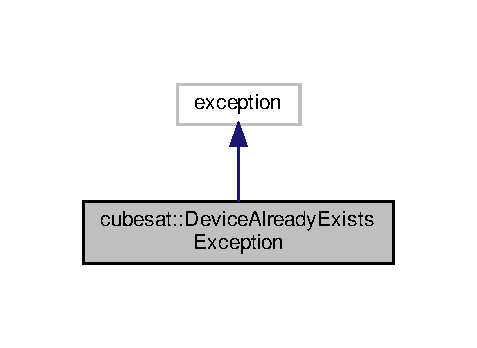
\includegraphics[width=229pt]{classcubesat_1_1DeviceAlreadyExistsException__inherit__graph}
\end{center}
\end{figure}


Collaboration diagram for cubesat\+:\+:Device\+Already\+Exists\+Exception\+:\nopagebreak
\begin{figure}[H]
\begin{center}
\leavevmode
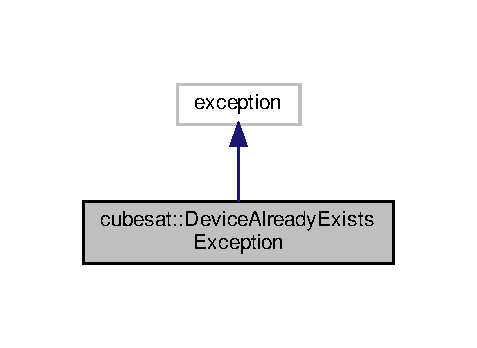
\includegraphics[width=229pt]{classcubesat_1_1DeviceAlreadyExistsException__coll__graph}
\end{center}
\end{figure}
\subsection*{Public Member Functions}
\begin{DoxyCompactItemize}
\item 
\hyperlink{classcubesat_1_1DeviceAlreadyExistsException_a98774fd7ef2f0c8ae21834aa31509261}{Device\+Already\+Exists\+Exception} (const std\+::string \&device\+\_\+name)
\item 
virtual const char $\ast$ \hyperlink{classcubesat_1_1DeviceAlreadyExistsException_a414ac8b05f5219189998541c0e8c15c0}{what} () const  throw ()
\end{DoxyCompactItemize}
\subsection*{Private Attributes}
\begin{DoxyCompactItemize}
\item 
std\+::string \hyperlink{classcubesat_1_1DeviceAlreadyExistsException_a23f9b3de4f6d97af9997336d61f06f31}{error\+\_\+msg}
\end{DoxyCompactItemize}


\subsection{Detailed Description}
Thrown if the user attempts to create a device with a name that is already taken 

\subsection{Constructor \& Destructor Documentation}
\mbox{\Hypertarget{classcubesat_1_1DeviceAlreadyExistsException_a98774fd7ef2f0c8ae21834aa31509261}\label{classcubesat_1_1DeviceAlreadyExistsException_a98774fd7ef2f0c8ae21834aa31509261}} 
\index{cubesat\+::\+Device\+Already\+Exists\+Exception@{cubesat\+::\+Device\+Already\+Exists\+Exception}!Device\+Already\+Exists\+Exception@{Device\+Already\+Exists\+Exception}}
\index{Device\+Already\+Exists\+Exception@{Device\+Already\+Exists\+Exception}!cubesat\+::\+Device\+Already\+Exists\+Exception@{cubesat\+::\+Device\+Already\+Exists\+Exception}}
\subsubsection{\texorpdfstring{Device\+Already\+Exists\+Exception()}{DeviceAlreadyExistsException()}}
{\footnotesize\ttfamily cubesat\+::\+Device\+Already\+Exists\+Exception\+::\+Device\+Already\+Exists\+Exception (\begin{DoxyParamCaption}\item[{const std\+::string \&}]{device\+\_\+name }\end{DoxyParamCaption})\hspace{0.3cm}{\ttfamily [inline]}}



\subsection{Member Function Documentation}
\mbox{\Hypertarget{classcubesat_1_1DeviceAlreadyExistsException_a414ac8b05f5219189998541c0e8c15c0}\label{classcubesat_1_1DeviceAlreadyExistsException_a414ac8b05f5219189998541c0e8c15c0}} 
\index{cubesat\+::\+Device\+Already\+Exists\+Exception@{cubesat\+::\+Device\+Already\+Exists\+Exception}!what@{what}}
\index{what@{what}!cubesat\+::\+Device\+Already\+Exists\+Exception@{cubesat\+::\+Device\+Already\+Exists\+Exception}}
\subsubsection{\texorpdfstring{what()}{what()}}
{\footnotesize\ttfamily virtual const char$\ast$ cubesat\+::\+Device\+Already\+Exists\+Exception\+::what (\begin{DoxyParamCaption}{ }\end{DoxyParamCaption}) const throw  ) \hspace{0.3cm}{\ttfamily [inline]}, {\ttfamily [virtual]}}



\subsection{Member Data Documentation}
\mbox{\Hypertarget{classcubesat_1_1DeviceAlreadyExistsException_a23f9b3de4f6d97af9997336d61f06f31}\label{classcubesat_1_1DeviceAlreadyExistsException_a23f9b3de4f6d97af9997336d61f06f31}} 
\index{cubesat\+::\+Device\+Already\+Exists\+Exception@{cubesat\+::\+Device\+Already\+Exists\+Exception}!error\+\_\+msg@{error\+\_\+msg}}
\index{error\+\_\+msg@{error\+\_\+msg}!cubesat\+::\+Device\+Already\+Exists\+Exception@{cubesat\+::\+Device\+Already\+Exists\+Exception}}
\subsubsection{\texorpdfstring{error\+\_\+msg}{error\_msg}}
{\footnotesize\ttfamily std\+::string cubesat\+::\+Device\+Already\+Exists\+Exception\+::error\+\_\+msg\hspace{0.3cm}{\ttfamily [private]}}



The documentation for this class was generated from the following file\+:\begin{DoxyCompactItemize}
\item 
/home/osboxes/cosmos/source/projects/cubesat-\/kit/include/utility/\hyperlink{Exceptions_8h}{Exceptions.\+h}\end{DoxyCompactItemize}

\hypertarget{unioncubesat_1_1OPT3001_1_1DeviceID}{}\section{cubesat\+:\+:O\+P\+T3001\+:\+:Device\+ID Union Reference}
\label{unioncubesat_1_1OPT3001_1_1DeviceID}\index{cubesat\+::\+O\+P\+T3001\+::\+Device\+ID@{cubesat\+::\+O\+P\+T3001\+::\+Device\+ID}}


Stores data pulled from the result register.  




{\ttfamily \#include $<$O\+P\+T3001.\+h$>$}

\subsection*{Public Attributes}
\begin{DoxyCompactItemize}
\item 
uint16\+\_\+t \hyperlink{unioncubesat_1_1OPT3001_1_1DeviceID_a07b4ae0da0b4162505e0e39131c7df95}{raw\+\_\+data}
\item 
\begin{tabbing}
xx\=xx\=xx\=xx\=xx\=xx\=xx\=xx\=xx\=\kill
struct \{\\
\>uint16\_t \hyperlink{unioncubesat_1_1OPT3001_1_1DeviceID_aca9343080bb1903c2ef7c8a8b1e980e9}{result}: 12\\
\}; \\

\end{tabbing}\end{DoxyCompactItemize}


\subsection{Detailed Description}
Stores data pulled from the result register. 

\subsection{Member Data Documentation}
\mbox{\Hypertarget{unioncubesat_1_1OPT3001_1_1DeviceID_ad92a3d1a63e939ebb55d6c97cf7ebffe}\label{unioncubesat_1_1OPT3001_1_1DeviceID_ad92a3d1a63e939ebb55d6c97cf7ebffe}} 
\subsubsection{\texorpdfstring{"@11}{@11}}
{\footnotesize\ttfamily struct \{ ... \} }

\mbox{\Hypertarget{unioncubesat_1_1OPT3001_1_1DeviceID_a07b4ae0da0b4162505e0e39131c7df95}\label{unioncubesat_1_1OPT3001_1_1DeviceID_a07b4ae0da0b4162505e0e39131c7df95}} 
\index{cubesat\+::\+O\+P\+T3001\+::\+Device\+ID@{cubesat\+::\+O\+P\+T3001\+::\+Device\+ID}!raw\+\_\+data@{raw\+\_\+data}}
\index{raw\+\_\+data@{raw\+\_\+data}!cubesat\+::\+O\+P\+T3001\+::\+Device\+ID@{cubesat\+::\+O\+P\+T3001\+::\+Device\+ID}}
\subsubsection{\texorpdfstring{raw\+\_\+data}{raw\_data}}
{\footnotesize\ttfamily uint16\+\_\+t cubesat\+::\+O\+P\+T3001\+::\+Device\+I\+D\+::raw\+\_\+data}

\mbox{\Hypertarget{unioncubesat_1_1OPT3001_1_1DeviceID_aca9343080bb1903c2ef7c8a8b1e980e9}\label{unioncubesat_1_1OPT3001_1_1DeviceID_aca9343080bb1903c2ef7c8a8b1e980e9}} 
\index{cubesat\+::\+O\+P\+T3001\+::\+Device\+ID@{cubesat\+::\+O\+P\+T3001\+::\+Device\+ID}!result@{result}}
\index{result@{result}!cubesat\+::\+O\+P\+T3001\+::\+Device\+ID@{cubesat\+::\+O\+P\+T3001\+::\+Device\+ID}}
\subsubsection{\texorpdfstring{result}{result}}
{\footnotesize\ttfamily uint16\+\_\+t cubesat\+::\+O\+P\+T3001\+::\+Device\+I\+D\+::result}



The documentation for this union was generated from the following file\+:\begin{DoxyCompactItemize}
\item 
/home/osboxes/cosmos/source/projects/cubesat-\/kit/include/device/\hyperlink{OPT3001_8h}{O\+P\+T3001.\+h}\end{DoxyCompactItemize}

\hypertarget{structcubesat_1_1DeviceImplBase}{}\section{cubesat\+:\+:Device\+Impl\+Base$<$ Device\+Struc\+Type, type\+\_\+ $>$ Struct Template Reference}
\label{structcubesat_1_1DeviceImplBase}\index{cubesat\+::\+Device\+Impl\+Base$<$ Device\+Struc\+Type, type\+\_\+ $>$@{cubesat\+::\+Device\+Impl\+Base$<$ Device\+Struc\+Type, type\+\_\+ $>$}}


{\ttfamily \#include $<$Device.\+h$>$}

\subsection*{Public Types}
\begin{DoxyCompactItemize}
\item 
using \hyperlink{structcubesat_1_1DeviceImplBase_a3b5c876c695495c8af41d14d7e15c37d}{\+\_\+\+\_\+\+Device\+Struc} = Device\+Struc\+Type
\end{DoxyCompactItemize}
\subsection*{Static Public Attributes}
\begin{DoxyCompactItemize}
\item 
static constexpr Device\+Type \hyperlink{structcubesat_1_1DeviceImplBase_a89e98fe7649db65d02679b06aa84d7c9}{type} = type\+\_\+
\end{DoxyCompactItemize}


\subsection{Member Typedef Documentation}
\mbox{\Hypertarget{structcubesat_1_1DeviceImplBase_a3b5c876c695495c8af41d14d7e15c37d}\label{structcubesat_1_1DeviceImplBase_a3b5c876c695495c8af41d14d7e15c37d}} 
\index{cubesat\+::\+Device\+Impl\+Base@{cubesat\+::\+Device\+Impl\+Base}!\+\_\+\+\_\+\+Device\+Struc@{\+\_\+\+\_\+\+Device\+Struc}}
\index{\+\_\+\+\_\+\+Device\+Struc@{\+\_\+\+\_\+\+Device\+Struc}!cubesat\+::\+Device\+Impl\+Base@{cubesat\+::\+Device\+Impl\+Base}}
\subsubsection{\texorpdfstring{\+\_\+\+\_\+\+Device\+Struc}{\_\_DeviceStruc}}
{\footnotesize\ttfamily template$<$typename Device\+Struc\+Type, Device\+Type type\+\_\+$>$ \\
using \hyperlink{structcubesat_1_1DeviceImplBase}{cubesat\+::\+Device\+Impl\+Base}$<$ Device\+Struc\+Type, type\+\_\+ $>$\+::\hyperlink{structcubesat_1_1DeviceImplBase_a3b5c876c695495c8af41d14d7e15c37d}{\+\_\+\+\_\+\+Device\+Struc} =  Device\+Struc\+Type}



\subsection{Member Data Documentation}
\mbox{\Hypertarget{structcubesat_1_1DeviceImplBase_a89e98fe7649db65d02679b06aa84d7c9}\label{structcubesat_1_1DeviceImplBase_a89e98fe7649db65d02679b06aa84d7c9}} 
\index{cubesat\+::\+Device\+Impl\+Base@{cubesat\+::\+Device\+Impl\+Base}!type@{type}}
\index{type@{type}!cubesat\+::\+Device\+Impl\+Base@{cubesat\+::\+Device\+Impl\+Base}}
\subsubsection{\texorpdfstring{type}{type}}
{\footnotesize\ttfamily template$<$typename Device\+Struc\+Type, Device\+Type type\+\_\+$>$ \\
constexpr Device\+Type \hyperlink{structcubesat_1_1DeviceImplBase}{cubesat\+::\+Device\+Impl\+Base}$<$ Device\+Struc\+Type, type\+\_\+ $>$\+::type = type\+\_\+\hspace{0.3cm}{\ttfamily [static]}}



The documentation for this struct was generated from the following file\+:\begin{DoxyCompactItemize}
\item 
/home/osboxes/cosmos/source/projects/cubesat-\/kit/include/utility/\hyperlink{Device_8h}{Device.\+h}\end{DoxyCompactItemize}

\hypertarget{classcubesat_1_1GPIO}{}\section{cubesat\+:\+:G\+P\+IO Class Reference}
\label{classcubesat_1_1GPIO}\index{cubesat\+::\+G\+P\+IO@{cubesat\+::\+G\+P\+IO}}


{\ttfamily \#include $<$G\+P\+I\+O.\+h$>$}



Inheritance diagram for cubesat\+:\+:G\+P\+IO\+:\nopagebreak
\begin{figure}[H]
\begin{center}
\leavevmode
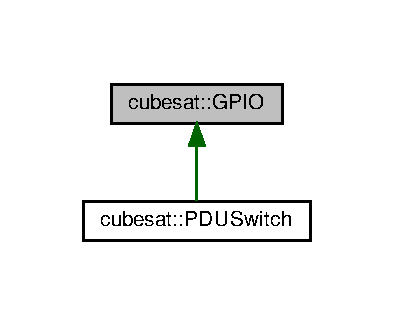
\includegraphics[width=189pt]{classcubesat_1_1GPIO__inherit__graph}
\end{center}
\end{figure}


Collaboration diagram for cubesat\+:\+:G\+P\+IO\+:\nopagebreak
\begin{figure}[H]
\begin{center}
\leavevmode
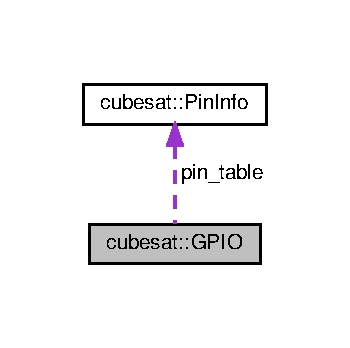
\includegraphics[width=168pt]{classcubesat_1_1GPIO__coll__graph}
\end{center}
\end{figure}
\subsection*{Public Member Functions}
\begin{DoxyCompactItemize}
\item 
\hyperlink{classcubesat_1_1GPIO_ae37721459fb7d477c095f60daaf3cd58}{G\+P\+IO} ()
\item 
\hyperlink{classcubesat_1_1GPIO_aeacb853859e7ca4d8d72999bc0cffb0f}{G\+P\+IO} (\hyperlink{namespacecubesat_af928ed4b56ef60d75953a91225b37a00}{Pin} \hyperlink{classcubesat_1_1GPIO_af3e219ff169f027626becf1797a02c50}{pin})
\item 
\hyperlink{classcubesat_1_1GPIO_aab35cd38f7fb1cec4ee7c5b1ff4adc13}{G\+P\+IO} (const char $\ast$pin\+\_\+key)
\item 
virtual \hyperlink{classcubesat_1_1GPIO_ae8205f95f108a15a612485b6358031a1}{$\sim$\+G\+P\+IO} ()
\item 
\hyperlink{namespacecubesat_a0c9368193169b1a4ca3aa1ba47331abf}{G\+P\+I\+O\+Mode} \hyperlink{classcubesat_1_1GPIO_a1aacbbd48883285a4730ec7167b1487d}{Set\+Mode} (\hyperlink{namespacecubesat_a0c9368193169b1a4ca3aa1ba47331abf}{G\+P\+I\+O\+Mode} mode)
\item 
\hyperlink{namespacecubesat_a0c9368193169b1a4ca3aa1ba47331abf}{G\+P\+I\+O\+Mode} \hyperlink{classcubesat_1_1GPIO_a6c9fa56927c168d8db8b1dd62fbc4cde}{Get\+Mode} ()
\item 
\hyperlink{namespacecubesat_ac60a35ee01913deca5e771944eb902ed}{G\+P\+I\+O\+Value} \hyperlink{classcubesat_1_1GPIO_a27eaf22ac52502400ffeddf7c90506ed}{Digital\+Write} (\hyperlink{namespacecubesat_ac60a35ee01913deca5e771944eb902ed}{G\+P\+I\+O\+Value} value)
\item 
\hyperlink{namespacecubesat_ac60a35ee01913deca5e771944eb902ed}{G\+P\+I\+O\+Value} \hyperlink{classcubesat_1_1GPIO_a427ef463f54d768e8d9b6abc449c5d9f}{Digital\+Read} ()
\item 
const char $\ast$ \hyperlink{classcubesat_1_1GPIO_af6aca76f5db71a14b69157360f7c070d}{Get\+Pin\+Key} () const
\item 
int \hyperlink{classcubesat_1_1GPIO_a865c8e0987a8f728a42aa5e2d9dd2241}{Get\+Pin\+Number} () const
\end{DoxyCompactItemize}
\subsection*{Static Public Member Functions}
\begin{DoxyCompactItemize}
\item 
static \hyperlink{namespacecubesat_af928ed4b56ef60d75953a91225b37a00}{Pin} \hyperlink{classcubesat_1_1GPIO_a0681d886f2a688683575716119e4af7a}{Get\+Pin\+By\+Key} (const char $\ast$key)
\item 
static \hyperlink{namespacecubesat_af928ed4b56ef60d75953a91225b37a00}{Pin} \hyperlink{classcubesat_1_1GPIO_afaa49b223ab1f338d279938a826eba2d}{Get\+Pin\+By\+Name} (const char $\ast$name)
\item 
static const char $\ast$ \hyperlink{classcubesat_1_1GPIO_a676a794c2d2f2f636c7a23f71613e48e}{Get\+Name\+By\+Pin} (\hyperlink{namespacecubesat_af928ed4b56ef60d75953a91225b37a00}{Pin} \hyperlink{classcubesat_1_1GPIO_af3e219ff169f027626becf1797a02c50}{pin})
\item 
static const char $\ast$ \hyperlink{classcubesat_1_1GPIO_a3df734f0471cf7e7038c186c80b14995}{Get\+Key\+By\+Pin} (\hyperlink{namespacecubesat_af928ed4b56ef60d75953a91225b37a00}{Pin} \hyperlink{classcubesat_1_1GPIO_af3e219ff169f027626becf1797a02c50}{pin})
\end{DoxyCompactItemize}
\subsection*{Protected Attributes}
\begin{DoxyCompactItemize}
\item 
\hyperlink{namespacecubesat_af928ed4b56ef60d75953a91225b37a00}{Pin} \hyperlink{classcubesat_1_1GPIO_af3e219ff169f027626becf1797a02c50}{pin}
\end{DoxyCompactItemize}
\subsection*{Static Protected Attributes}
\begin{DoxyCompactItemize}
\item 
static \hyperlink{structcubesat_1_1PinInfo}{Pin\+Info} \hyperlink{classcubesat_1_1GPIO_a799d772718448f641fa2d4a3a18e60ac}{pin\+\_\+table} \mbox{[}97\mbox{]}
\end{DoxyCompactItemize}


\subsection{Constructor \& Destructor Documentation}
\mbox{\Hypertarget{classcubesat_1_1GPIO_ae37721459fb7d477c095f60daaf3cd58}\label{classcubesat_1_1GPIO_ae37721459fb7d477c095f60daaf3cd58}} 
\index{cubesat\+::\+G\+P\+IO@{cubesat\+::\+G\+P\+IO}!G\+P\+IO@{G\+P\+IO}}
\index{G\+P\+IO@{G\+P\+IO}!cubesat\+::\+G\+P\+IO@{cubesat\+::\+G\+P\+IO}}
\subsubsection{\texorpdfstring{G\+P\+I\+O()}{GPIO()}\hspace{0.1cm}{\footnotesize\ttfamily [1/3]}}
{\footnotesize\ttfamily cubesat\+::\+G\+P\+I\+O\+::\+G\+P\+IO (\begin{DoxyParamCaption}{ }\end{DoxyParamCaption})\hspace{0.3cm}{\ttfamily [inline]}}

\mbox{\Hypertarget{classcubesat_1_1GPIO_aeacb853859e7ca4d8d72999bc0cffb0f}\label{classcubesat_1_1GPIO_aeacb853859e7ca4d8d72999bc0cffb0f}} 
\index{cubesat\+::\+G\+P\+IO@{cubesat\+::\+G\+P\+IO}!G\+P\+IO@{G\+P\+IO}}
\index{G\+P\+IO@{G\+P\+IO}!cubesat\+::\+G\+P\+IO@{cubesat\+::\+G\+P\+IO}}
\subsubsection{\texorpdfstring{G\+P\+I\+O()}{GPIO()}\hspace{0.1cm}{\footnotesize\ttfamily [2/3]}}
{\footnotesize\ttfamily G\+P\+I\+O\+::\+G\+P\+IO (\begin{DoxyParamCaption}\item[{\hyperlink{namespacecubesat_af928ed4b56ef60d75953a91225b37a00}{Pin}}]{pin }\end{DoxyParamCaption})}

\mbox{\Hypertarget{classcubesat_1_1GPIO_aab35cd38f7fb1cec4ee7c5b1ff4adc13}\label{classcubesat_1_1GPIO_aab35cd38f7fb1cec4ee7c5b1ff4adc13}} 
\index{cubesat\+::\+G\+P\+IO@{cubesat\+::\+G\+P\+IO}!G\+P\+IO@{G\+P\+IO}}
\index{G\+P\+IO@{G\+P\+IO}!cubesat\+::\+G\+P\+IO@{cubesat\+::\+G\+P\+IO}}
\subsubsection{\texorpdfstring{G\+P\+I\+O()}{GPIO()}\hspace{0.1cm}{\footnotesize\ttfamily [3/3]}}
{\footnotesize\ttfamily G\+P\+I\+O\+::\+G\+P\+IO (\begin{DoxyParamCaption}\item[{const char $\ast$}]{pin\+\_\+key }\end{DoxyParamCaption})}

\mbox{\Hypertarget{classcubesat_1_1GPIO_ae8205f95f108a15a612485b6358031a1}\label{classcubesat_1_1GPIO_ae8205f95f108a15a612485b6358031a1}} 
\index{cubesat\+::\+G\+P\+IO@{cubesat\+::\+G\+P\+IO}!````~G\+P\+IO@{$\sim$\+G\+P\+IO}}
\index{````~G\+P\+IO@{$\sim$\+G\+P\+IO}!cubesat\+::\+G\+P\+IO@{cubesat\+::\+G\+P\+IO}}
\subsubsection{\texorpdfstring{$\sim$\+G\+P\+I\+O()}{~GPIO()}}
{\footnotesize\ttfamily G\+P\+I\+O\+::$\sim$\+G\+P\+IO (\begin{DoxyParamCaption}{ }\end{DoxyParamCaption})\hspace{0.3cm}{\ttfamily [virtual]}}



\subsection{Member Function Documentation}
\mbox{\Hypertarget{classcubesat_1_1GPIO_a427ef463f54d768e8d9b6abc449c5d9f}\label{classcubesat_1_1GPIO_a427ef463f54d768e8d9b6abc449c5d9f}} 
\index{cubesat\+::\+G\+P\+IO@{cubesat\+::\+G\+P\+IO}!Digital\+Read@{Digital\+Read}}
\index{Digital\+Read@{Digital\+Read}!cubesat\+::\+G\+P\+IO@{cubesat\+::\+G\+P\+IO}}
\subsubsection{\texorpdfstring{Digital\+Read()}{DigitalRead()}}
{\footnotesize\ttfamily \hyperlink{namespacecubesat_ac60a35ee01913deca5e771944eb902ed}{G\+P\+I\+O\+Value} G\+P\+I\+O\+::\+Digital\+Read (\begin{DoxyParamCaption}{ }\end{DoxyParamCaption})}

\mbox{\Hypertarget{classcubesat_1_1GPIO_a27eaf22ac52502400ffeddf7c90506ed}\label{classcubesat_1_1GPIO_a27eaf22ac52502400ffeddf7c90506ed}} 
\index{cubesat\+::\+G\+P\+IO@{cubesat\+::\+G\+P\+IO}!Digital\+Write@{Digital\+Write}}
\index{Digital\+Write@{Digital\+Write}!cubesat\+::\+G\+P\+IO@{cubesat\+::\+G\+P\+IO}}
\subsubsection{\texorpdfstring{Digital\+Write()}{DigitalWrite()}}
{\footnotesize\ttfamily \hyperlink{namespacecubesat_ac60a35ee01913deca5e771944eb902ed}{G\+P\+I\+O\+Value} G\+P\+I\+O\+::\+Digital\+Write (\begin{DoxyParamCaption}\item[{\hyperlink{namespacecubesat_ac60a35ee01913deca5e771944eb902ed}{G\+P\+I\+O\+Value}}]{value }\end{DoxyParamCaption})}

\mbox{\Hypertarget{classcubesat_1_1GPIO_a3df734f0471cf7e7038c186c80b14995}\label{classcubesat_1_1GPIO_a3df734f0471cf7e7038c186c80b14995}} 
\index{cubesat\+::\+G\+P\+IO@{cubesat\+::\+G\+P\+IO}!Get\+Key\+By\+Pin@{Get\+Key\+By\+Pin}}
\index{Get\+Key\+By\+Pin@{Get\+Key\+By\+Pin}!cubesat\+::\+G\+P\+IO@{cubesat\+::\+G\+P\+IO}}
\subsubsection{\texorpdfstring{Get\+Key\+By\+Pin()}{GetKeyByPin()}}
{\footnotesize\ttfamily const char $\ast$ G\+P\+I\+O\+::\+Get\+Key\+By\+Pin (\begin{DoxyParamCaption}\item[{\hyperlink{namespacecubesat_af928ed4b56ef60d75953a91225b37a00}{Pin}}]{pin }\end{DoxyParamCaption})\hspace{0.3cm}{\ttfamily [static]}}

\mbox{\Hypertarget{classcubesat_1_1GPIO_a6c9fa56927c168d8db8b1dd62fbc4cde}\label{classcubesat_1_1GPIO_a6c9fa56927c168d8db8b1dd62fbc4cde}} 
\index{cubesat\+::\+G\+P\+IO@{cubesat\+::\+G\+P\+IO}!Get\+Mode@{Get\+Mode}}
\index{Get\+Mode@{Get\+Mode}!cubesat\+::\+G\+P\+IO@{cubesat\+::\+G\+P\+IO}}
\subsubsection{\texorpdfstring{Get\+Mode()}{GetMode()}}
{\footnotesize\ttfamily \hyperlink{namespacecubesat_a0c9368193169b1a4ca3aa1ba47331abf}{G\+P\+I\+O\+Mode} G\+P\+I\+O\+::\+Get\+Mode (\begin{DoxyParamCaption}{ }\end{DoxyParamCaption})}

\mbox{\Hypertarget{classcubesat_1_1GPIO_a676a794c2d2f2f636c7a23f71613e48e}\label{classcubesat_1_1GPIO_a676a794c2d2f2f636c7a23f71613e48e}} 
\index{cubesat\+::\+G\+P\+IO@{cubesat\+::\+G\+P\+IO}!Get\+Name\+By\+Pin@{Get\+Name\+By\+Pin}}
\index{Get\+Name\+By\+Pin@{Get\+Name\+By\+Pin}!cubesat\+::\+G\+P\+IO@{cubesat\+::\+G\+P\+IO}}
\subsubsection{\texorpdfstring{Get\+Name\+By\+Pin()}{GetNameByPin()}}
{\footnotesize\ttfamily const char $\ast$ G\+P\+I\+O\+::\+Get\+Name\+By\+Pin (\begin{DoxyParamCaption}\item[{\hyperlink{namespacecubesat_af928ed4b56ef60d75953a91225b37a00}{Pin}}]{pin }\end{DoxyParamCaption})\hspace{0.3cm}{\ttfamily [static]}}

\mbox{\Hypertarget{classcubesat_1_1GPIO_a0681d886f2a688683575716119e4af7a}\label{classcubesat_1_1GPIO_a0681d886f2a688683575716119e4af7a}} 
\index{cubesat\+::\+G\+P\+IO@{cubesat\+::\+G\+P\+IO}!Get\+Pin\+By\+Key@{Get\+Pin\+By\+Key}}
\index{Get\+Pin\+By\+Key@{Get\+Pin\+By\+Key}!cubesat\+::\+G\+P\+IO@{cubesat\+::\+G\+P\+IO}}
\subsubsection{\texorpdfstring{Get\+Pin\+By\+Key()}{GetPinByKey()}}
{\footnotesize\ttfamily \hyperlink{namespacecubesat_af928ed4b56ef60d75953a91225b37a00}{Pin} G\+P\+I\+O\+::\+Get\+Pin\+By\+Key (\begin{DoxyParamCaption}\item[{const char $\ast$}]{key }\end{DoxyParamCaption})\hspace{0.3cm}{\ttfamily [static]}}

\mbox{\Hypertarget{classcubesat_1_1GPIO_afaa49b223ab1f338d279938a826eba2d}\label{classcubesat_1_1GPIO_afaa49b223ab1f338d279938a826eba2d}} 
\index{cubesat\+::\+G\+P\+IO@{cubesat\+::\+G\+P\+IO}!Get\+Pin\+By\+Name@{Get\+Pin\+By\+Name}}
\index{Get\+Pin\+By\+Name@{Get\+Pin\+By\+Name}!cubesat\+::\+G\+P\+IO@{cubesat\+::\+G\+P\+IO}}
\subsubsection{\texorpdfstring{Get\+Pin\+By\+Name()}{GetPinByName()}}
{\footnotesize\ttfamily \hyperlink{namespacecubesat_af928ed4b56ef60d75953a91225b37a00}{Pin} G\+P\+I\+O\+::\+Get\+Pin\+By\+Name (\begin{DoxyParamCaption}\item[{const char $\ast$}]{name }\end{DoxyParamCaption})\hspace{0.3cm}{\ttfamily [static]}}

\mbox{\Hypertarget{classcubesat_1_1GPIO_af6aca76f5db71a14b69157360f7c070d}\label{classcubesat_1_1GPIO_af6aca76f5db71a14b69157360f7c070d}} 
\index{cubesat\+::\+G\+P\+IO@{cubesat\+::\+G\+P\+IO}!Get\+Pin\+Key@{Get\+Pin\+Key}}
\index{Get\+Pin\+Key@{Get\+Pin\+Key}!cubesat\+::\+G\+P\+IO@{cubesat\+::\+G\+P\+IO}}
\subsubsection{\texorpdfstring{Get\+Pin\+Key()}{GetPinKey()}}
{\footnotesize\ttfamily const char$\ast$ cubesat\+::\+G\+P\+I\+O\+::\+Get\+Pin\+Key (\begin{DoxyParamCaption}{ }\end{DoxyParamCaption}) const\hspace{0.3cm}{\ttfamily [inline]}}

\mbox{\Hypertarget{classcubesat_1_1GPIO_a865c8e0987a8f728a42aa5e2d9dd2241}\label{classcubesat_1_1GPIO_a865c8e0987a8f728a42aa5e2d9dd2241}} 
\index{cubesat\+::\+G\+P\+IO@{cubesat\+::\+G\+P\+IO}!Get\+Pin\+Number@{Get\+Pin\+Number}}
\index{Get\+Pin\+Number@{Get\+Pin\+Number}!cubesat\+::\+G\+P\+IO@{cubesat\+::\+G\+P\+IO}}
\subsubsection{\texorpdfstring{Get\+Pin\+Number()}{GetPinNumber()}}
{\footnotesize\ttfamily int cubesat\+::\+G\+P\+I\+O\+::\+Get\+Pin\+Number (\begin{DoxyParamCaption}{ }\end{DoxyParamCaption}) const\hspace{0.3cm}{\ttfamily [inline]}}

\mbox{\Hypertarget{classcubesat_1_1GPIO_a1aacbbd48883285a4730ec7167b1487d}\label{classcubesat_1_1GPIO_a1aacbbd48883285a4730ec7167b1487d}} 
\index{cubesat\+::\+G\+P\+IO@{cubesat\+::\+G\+P\+IO}!Set\+Mode@{Set\+Mode}}
\index{Set\+Mode@{Set\+Mode}!cubesat\+::\+G\+P\+IO@{cubesat\+::\+G\+P\+IO}}
\subsubsection{\texorpdfstring{Set\+Mode()}{SetMode()}}
{\footnotesize\ttfamily \hyperlink{namespacecubesat_a0c9368193169b1a4ca3aa1ba47331abf}{G\+P\+I\+O\+Mode} G\+P\+I\+O\+::\+Set\+Mode (\begin{DoxyParamCaption}\item[{\hyperlink{namespacecubesat_a0c9368193169b1a4ca3aa1ba47331abf}{G\+P\+I\+O\+Mode}}]{mode }\end{DoxyParamCaption})}



\subsection{Member Data Documentation}
\mbox{\Hypertarget{classcubesat_1_1GPIO_af3e219ff169f027626becf1797a02c50}\label{classcubesat_1_1GPIO_af3e219ff169f027626becf1797a02c50}} 
\index{cubesat\+::\+G\+P\+IO@{cubesat\+::\+G\+P\+IO}!pin@{pin}}
\index{pin@{pin}!cubesat\+::\+G\+P\+IO@{cubesat\+::\+G\+P\+IO}}
\subsubsection{\texorpdfstring{pin}{pin}}
{\footnotesize\ttfamily \hyperlink{namespacecubesat_af928ed4b56ef60d75953a91225b37a00}{Pin} cubesat\+::\+G\+P\+I\+O\+::pin\hspace{0.3cm}{\ttfamily [protected]}}

\mbox{\Hypertarget{classcubesat_1_1GPIO_a799d772718448f641fa2d4a3a18e60ac}\label{classcubesat_1_1GPIO_a799d772718448f641fa2d4a3a18e60ac}} 
\index{cubesat\+::\+G\+P\+IO@{cubesat\+::\+G\+P\+IO}!pin\+\_\+table@{pin\+\_\+table}}
\index{pin\+\_\+table@{pin\+\_\+table}!cubesat\+::\+G\+P\+IO@{cubesat\+::\+G\+P\+IO}}
\subsubsection{\texorpdfstring{pin\+\_\+table}{pin\_table}}
{\footnotesize\ttfamily \hyperlink{structcubesat_1_1PinInfo}{Pin\+Info} G\+P\+I\+O\+::pin\+\_\+table\hspace{0.3cm}{\ttfamily [static]}, {\ttfamily [protected]}}



The documentation for this class was generated from the following files\+:\begin{DoxyCompactItemize}
\item 
/home/osboxes/cosmos/source/projects/cubesat-\/kit/include/device/\hyperlink{GPIO_8h}{G\+P\+I\+O.\+h}\item 
/home/osboxes/cosmos/source/projects/cubesat-\/kit/source/device/\hyperlink{GPIO_8cpp}{G\+P\+I\+O.\+cpp}\end{DoxyCompactItemize}

\hypertarget{classcubesat_1_1GPS}{}\section{cubesat\+:\+:G\+PS Class Reference}
\label{classcubesat_1_1GPS}\index{cubesat\+::\+G\+PS@{cubesat\+::\+G\+PS}}


{\ttfamily \#include $<$Device.\+h$>$}



Inheritance diagram for cubesat\+:\+:G\+PS\+:
\nopagebreak
\begin{figure}[H]
\begin{center}
\leavevmode
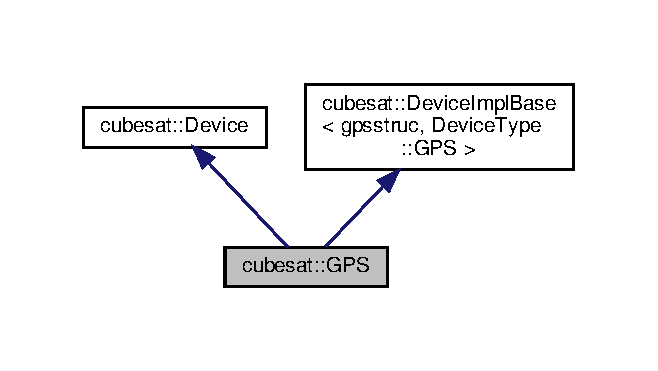
\includegraphics[width=316pt]{classcubesat_1_1GPS__inherit__graph}
\end{center}
\end{figure}


Collaboration diagram for cubesat\+:\+:G\+PS\+:
\nopagebreak
\begin{figure}[H]
\begin{center}
\leavevmode
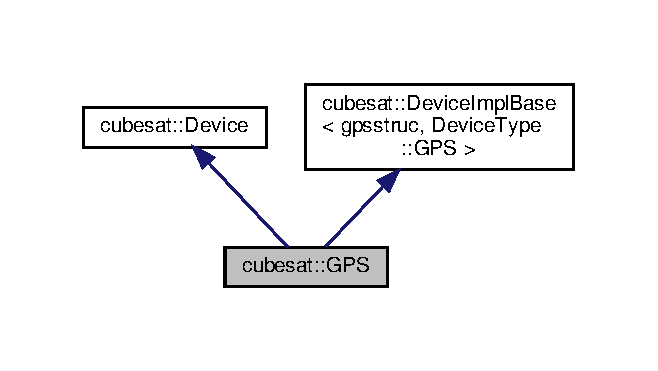
\includegraphics[width=316pt]{classcubesat_1_1GPS__coll__graph}
\end{center}
\end{figure}
\subsection*{Public Member Functions}
\begin{DoxyCompactItemize}
\item 
\hyperlink{classcubesat_1_1GPS_a033475ed836181ce17e2280a0ac6c78a}{G\+PS} (Agent $\ast$\hyperlink{classcubesat_1_1Device_a8499108eccaf7375bea8ead0182391a6}{agent}, int \hyperlink{classcubesat_1_1Device_a1deca725b01f8ef37e49662da6db4e53}{cindex}, int \hyperlink{classcubesat_1_1Device_a8a2b3d6d7400e6796c31705058172982}{dindex})
\item 
virtual \hyperlink{classcubesat_1_1GPS_a85ee6eba278200dddd5587c4cf2944fd}{$\sim$\+G\+PS} ()
\item 
\hyperlink{classcubesat_1_1GPS_ad360460187cc59936dd5b3be9e910cf3}{\+\_\+\+Add\+Property} (temperature, temp)
\item 
\hyperlink{classcubesat_1_1GPS_a0e85bdda2dc5cfcd0d637743ee8c9d0a}{\+\_\+\+Add\+Property} (utc, utc)
\item 
\hyperlink{classcubesat_1_1GPS_ac76d9e1915875a65690dffde32ef8618}{\+\_\+\+Add\+Property} (voltage, volt)
\item 
\hyperlink{classcubesat_1_1GPS_a55cc7f5abbd30fb9d1411718eb31b5a0}{\+\_\+\+Add\+Property} (current, amp)
\item 
\hyperlink{classcubesat_1_1GPS_a56c7d2ec1d4d8d93349d7a39b0de0346}{\+\_\+\+Add\+Property} (power, power)
\item 
\hyperlink{classcubesat_1_1GPS_afc908fc649610221f240f583baf18e7d}{\+\_\+\+Add\+Property} (enabled, enabled)
\item 
\hyperlink{classcubesat_1_1GPS_a525f1fcbadb25e45fe71ea5ac8ec5dd9}{\+\_\+\+Add\+Property} (satellites\+\_\+used, sats\+\_\+used)
\item 
\hyperlink{classcubesat_1_1GPS_a66df85c7601286f73b82d561b0755686}{\+\_\+\+Add\+Property} (location, geods)
\item 
\hyperlink{classcubesat_1_1GPS_a0e881f5aa0f080d69da97a0b03b35c5d}{\+\_\+\+Add\+Property} (velocity, geocv)
\end{DoxyCompactItemize}
\subsection*{Additional Inherited Members}


\subsection{Constructor \& Destructor Documentation}
\mbox{\Hypertarget{classcubesat_1_1GPS_a033475ed836181ce17e2280a0ac6c78a}\label{classcubesat_1_1GPS_a033475ed836181ce17e2280a0ac6c78a}} 
\index{cubesat\+::\+G\+PS@{cubesat\+::\+G\+PS}!G\+PS@{G\+PS}}
\index{G\+PS@{G\+PS}!cubesat\+::\+G\+PS@{cubesat\+::\+G\+PS}}
\subsubsection{\texorpdfstring{G\+P\+S()}{GPS()}}
{\footnotesize\ttfamily cubesat\+::\+G\+P\+S\+::\+G\+PS (\begin{DoxyParamCaption}\item[{Agent $\ast$}]{agent,  }\item[{int}]{cindex,  }\item[{int}]{dindex }\end{DoxyParamCaption})\hspace{0.3cm}{\ttfamily [inline]}}

\mbox{\Hypertarget{classcubesat_1_1GPS_a85ee6eba278200dddd5587c4cf2944fd}\label{classcubesat_1_1GPS_a85ee6eba278200dddd5587c4cf2944fd}} 
\index{cubesat\+::\+G\+PS@{cubesat\+::\+G\+PS}!````~G\+PS@{$\sim$\+G\+PS}}
\index{````~G\+PS@{$\sim$\+G\+PS}!cubesat\+::\+G\+PS@{cubesat\+::\+G\+PS}}
\subsubsection{\texorpdfstring{$\sim$\+G\+P\+S()}{~GPS()}}
{\footnotesize\ttfamily virtual cubesat\+::\+G\+P\+S\+::$\sim$\+G\+PS (\begin{DoxyParamCaption}{ }\end{DoxyParamCaption})\hspace{0.3cm}{\ttfamily [inline]}, {\ttfamily [virtual]}}



\subsection{Member Function Documentation}
\mbox{\Hypertarget{classcubesat_1_1GPS_ad360460187cc59936dd5b3be9e910cf3}\label{classcubesat_1_1GPS_ad360460187cc59936dd5b3be9e910cf3}} 
\index{cubesat\+::\+G\+PS@{cubesat\+::\+G\+PS}!\+\_\+\+Add\+Property@{\+\_\+\+Add\+Property}}
\index{\+\_\+\+Add\+Property@{\+\_\+\+Add\+Property}!cubesat\+::\+G\+PS@{cubesat\+::\+G\+PS}}
\subsubsection{\texorpdfstring{\+\_\+\+Add\+Property()}{\_AddProperty()}\hspace{0.1cm}{\footnotesize\ttfamily [1/9]}}
{\footnotesize\ttfamily cubesat\+::\+G\+P\+S\+::\+\_\+\+Add\+Property (\begin{DoxyParamCaption}\item[{temperature}]{,  }\item[{temp}]{ }\end{DoxyParamCaption})}

\mbox{\Hypertarget{classcubesat_1_1GPS_a0e85bdda2dc5cfcd0d637743ee8c9d0a}\label{classcubesat_1_1GPS_a0e85bdda2dc5cfcd0d637743ee8c9d0a}} 
\index{cubesat\+::\+G\+PS@{cubesat\+::\+G\+PS}!\+\_\+\+Add\+Property@{\+\_\+\+Add\+Property}}
\index{\+\_\+\+Add\+Property@{\+\_\+\+Add\+Property}!cubesat\+::\+G\+PS@{cubesat\+::\+G\+PS}}
\subsubsection{\texorpdfstring{\+\_\+\+Add\+Property()}{\_AddProperty()}\hspace{0.1cm}{\footnotesize\ttfamily [2/9]}}
{\footnotesize\ttfamily cubesat\+::\+G\+P\+S\+::\+\_\+\+Add\+Property (\begin{DoxyParamCaption}\item[{utc}]{,  }\item[{utc}]{ }\end{DoxyParamCaption})}

\mbox{\Hypertarget{classcubesat_1_1GPS_ac76d9e1915875a65690dffde32ef8618}\label{classcubesat_1_1GPS_ac76d9e1915875a65690dffde32ef8618}} 
\index{cubesat\+::\+G\+PS@{cubesat\+::\+G\+PS}!\+\_\+\+Add\+Property@{\+\_\+\+Add\+Property}}
\index{\+\_\+\+Add\+Property@{\+\_\+\+Add\+Property}!cubesat\+::\+G\+PS@{cubesat\+::\+G\+PS}}
\subsubsection{\texorpdfstring{\+\_\+\+Add\+Property()}{\_AddProperty()}\hspace{0.1cm}{\footnotesize\ttfamily [3/9]}}
{\footnotesize\ttfamily cubesat\+::\+G\+P\+S\+::\+\_\+\+Add\+Property (\begin{DoxyParamCaption}\item[{voltage}]{,  }\item[{volt}]{ }\end{DoxyParamCaption})}

\mbox{\Hypertarget{classcubesat_1_1GPS_a55cc7f5abbd30fb9d1411718eb31b5a0}\label{classcubesat_1_1GPS_a55cc7f5abbd30fb9d1411718eb31b5a0}} 
\index{cubesat\+::\+G\+PS@{cubesat\+::\+G\+PS}!\+\_\+\+Add\+Property@{\+\_\+\+Add\+Property}}
\index{\+\_\+\+Add\+Property@{\+\_\+\+Add\+Property}!cubesat\+::\+G\+PS@{cubesat\+::\+G\+PS}}
\subsubsection{\texorpdfstring{\+\_\+\+Add\+Property()}{\_AddProperty()}\hspace{0.1cm}{\footnotesize\ttfamily [4/9]}}
{\footnotesize\ttfamily cubesat\+::\+G\+P\+S\+::\+\_\+\+Add\+Property (\begin{DoxyParamCaption}\item[{current}]{,  }\item[{amp}]{ }\end{DoxyParamCaption})}

\mbox{\Hypertarget{classcubesat_1_1GPS_a56c7d2ec1d4d8d93349d7a39b0de0346}\label{classcubesat_1_1GPS_a56c7d2ec1d4d8d93349d7a39b0de0346}} 
\index{cubesat\+::\+G\+PS@{cubesat\+::\+G\+PS}!\+\_\+\+Add\+Property@{\+\_\+\+Add\+Property}}
\index{\+\_\+\+Add\+Property@{\+\_\+\+Add\+Property}!cubesat\+::\+G\+PS@{cubesat\+::\+G\+PS}}
\subsubsection{\texorpdfstring{\+\_\+\+Add\+Property()}{\_AddProperty()}\hspace{0.1cm}{\footnotesize\ttfamily [5/9]}}
{\footnotesize\ttfamily cubesat\+::\+G\+P\+S\+::\+\_\+\+Add\+Property (\begin{DoxyParamCaption}\item[{power}]{,  }\item[{power}]{ }\end{DoxyParamCaption})}

\mbox{\Hypertarget{classcubesat_1_1GPS_afc908fc649610221f240f583baf18e7d}\label{classcubesat_1_1GPS_afc908fc649610221f240f583baf18e7d}} 
\index{cubesat\+::\+G\+PS@{cubesat\+::\+G\+PS}!\+\_\+\+Add\+Property@{\+\_\+\+Add\+Property}}
\index{\+\_\+\+Add\+Property@{\+\_\+\+Add\+Property}!cubesat\+::\+G\+PS@{cubesat\+::\+G\+PS}}
\subsubsection{\texorpdfstring{\+\_\+\+Add\+Property()}{\_AddProperty()}\hspace{0.1cm}{\footnotesize\ttfamily [6/9]}}
{\footnotesize\ttfamily cubesat\+::\+G\+P\+S\+::\+\_\+\+Add\+Property (\begin{DoxyParamCaption}\item[{enabled}]{,  }\item[{enabled}]{ }\end{DoxyParamCaption})}

\mbox{\Hypertarget{classcubesat_1_1GPS_a525f1fcbadb25e45fe71ea5ac8ec5dd9}\label{classcubesat_1_1GPS_a525f1fcbadb25e45fe71ea5ac8ec5dd9}} 
\index{cubesat\+::\+G\+PS@{cubesat\+::\+G\+PS}!\+\_\+\+Add\+Property@{\+\_\+\+Add\+Property}}
\index{\+\_\+\+Add\+Property@{\+\_\+\+Add\+Property}!cubesat\+::\+G\+PS@{cubesat\+::\+G\+PS}}
\subsubsection{\texorpdfstring{\+\_\+\+Add\+Property()}{\_AddProperty()}\hspace{0.1cm}{\footnotesize\ttfamily [7/9]}}
{\footnotesize\ttfamily cubesat\+::\+G\+P\+S\+::\+\_\+\+Add\+Property (\begin{DoxyParamCaption}\item[{satellites\+\_\+used}]{,  }\item[{sats\+\_\+used}]{ }\end{DoxyParamCaption})}

\mbox{\Hypertarget{classcubesat_1_1GPS_a66df85c7601286f73b82d561b0755686}\label{classcubesat_1_1GPS_a66df85c7601286f73b82d561b0755686}} 
\index{cubesat\+::\+G\+PS@{cubesat\+::\+G\+PS}!\+\_\+\+Add\+Property@{\+\_\+\+Add\+Property}}
\index{\+\_\+\+Add\+Property@{\+\_\+\+Add\+Property}!cubesat\+::\+G\+PS@{cubesat\+::\+G\+PS}}
\subsubsection{\texorpdfstring{\+\_\+\+Add\+Property()}{\_AddProperty()}\hspace{0.1cm}{\footnotesize\ttfamily [8/9]}}
{\footnotesize\ttfamily cubesat\+::\+G\+P\+S\+::\+\_\+\+Add\+Property (\begin{DoxyParamCaption}\item[{location}]{,  }\item[{geods}]{ }\end{DoxyParamCaption})}

\mbox{\Hypertarget{classcubesat_1_1GPS_a0e881f5aa0f080d69da97a0b03b35c5d}\label{classcubesat_1_1GPS_a0e881f5aa0f080d69da97a0b03b35c5d}} 
\index{cubesat\+::\+G\+PS@{cubesat\+::\+G\+PS}!\+\_\+\+Add\+Property@{\+\_\+\+Add\+Property}}
\index{\+\_\+\+Add\+Property@{\+\_\+\+Add\+Property}!cubesat\+::\+G\+PS@{cubesat\+::\+G\+PS}}
\subsubsection{\texorpdfstring{\+\_\+\+Add\+Property()}{\_AddProperty()}\hspace{0.1cm}{\footnotesize\ttfamily [9/9]}}
{\footnotesize\ttfamily cubesat\+::\+G\+P\+S\+::\+\_\+\+Add\+Property (\begin{DoxyParamCaption}\item[{velocity}]{,  }\item[{geocv}]{ }\end{DoxyParamCaption})}



The documentation for this class was generated from the following file\+:\begin{DoxyCompactItemize}
\item 
/home/osboxes/cosmos/source/projects/cubesat-\/kit/include/utility/\hyperlink{Device_8h}{Device.\+h}\end{DoxyCompactItemize}

\hypertarget{classcubesat_1_1Heater}{}\section{cubesat\+:\+:Heater Class Reference}
\label{classcubesat_1_1Heater}\index{cubesat\+::\+Heater@{cubesat\+::\+Heater}}


{\ttfamily \#include $<$Device.\+h$>$}



Inheritance diagram for cubesat\+:\+:Heater\+:
\nopagebreak
\begin{figure}[H]
\begin{center}
\leavevmode
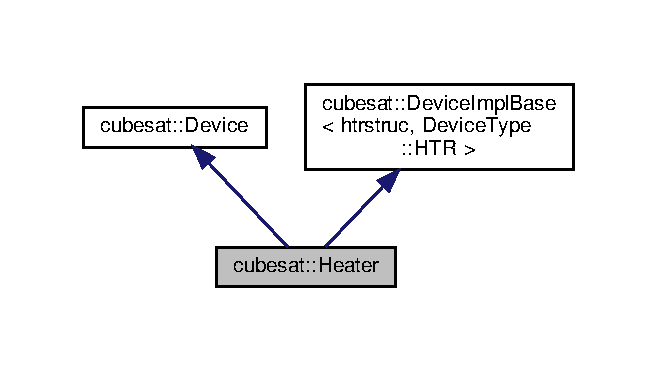
\includegraphics[width=316pt]{classcubesat_1_1Heater__inherit__graph}
\end{center}
\end{figure}


Collaboration diagram for cubesat\+:\+:Heater\+:
\nopagebreak
\begin{figure}[H]
\begin{center}
\leavevmode
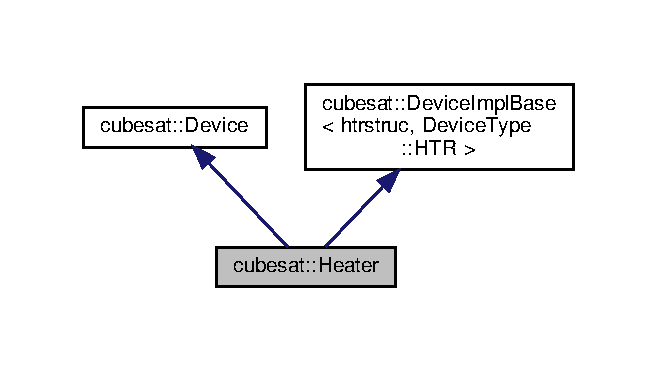
\includegraphics[width=316pt]{classcubesat_1_1Heater__coll__graph}
\end{center}
\end{figure}
\subsection*{Public Member Functions}
\begin{DoxyCompactItemize}
\item 
\hyperlink{classcubesat_1_1Heater_ad66d360dfab4e5b0a3b1ca61167295f3}{Heater} (Agent $\ast$\hyperlink{classcubesat_1_1Device_a8499108eccaf7375bea8ead0182391a6}{agent}, int \hyperlink{classcubesat_1_1Device_a1deca725b01f8ef37e49662da6db4e53}{cindex}, int \hyperlink{classcubesat_1_1Device_a8a2b3d6d7400e6796c31705058172982}{dindex})
\item 
virtual \hyperlink{classcubesat_1_1Heater_a806f58caf9b9a74c20d1a426f5b339e4}{$\sim$\+Heater} ()
\item 
\hyperlink{classcubesat_1_1Heater_ab8f6bb7b9d46622677e6fbf5f70a05d1}{\+\_\+\+Add\+Property} (utc, utc)
\begin{DoxyCompactList}\small\item\em The timestamp for this device. \end{DoxyCompactList}\item 
\hyperlink{classcubesat_1_1Heater_a98f2dda11d692b8dae418764e6efd865}{\+\_\+\+Add\+Property} (voltage, volt)
\item 
\hyperlink{classcubesat_1_1Heater_a0ed9b05c35f70645dcbb759d221553b6}{\+\_\+\+Add\+Property} (current, amp)
\item 
\hyperlink{classcubesat_1_1Heater_a0fc3d2d1e7be729233941badd87132dc}{\+\_\+\+Add\+Property} (power, power)
\item 
\hyperlink{classcubesat_1_1Heater_aec846009881794b1594b21544730e52e}{\+\_\+\+Add\+Property} (enabled, enabled)
\end{DoxyCompactItemize}
\subsection*{Additional Inherited Members}


\subsection{Constructor \& Destructor Documentation}
\mbox{\Hypertarget{classcubesat_1_1Heater_ad66d360dfab4e5b0a3b1ca61167295f3}\label{classcubesat_1_1Heater_ad66d360dfab4e5b0a3b1ca61167295f3}} 
\index{cubesat\+::\+Heater@{cubesat\+::\+Heater}!Heater@{Heater}}
\index{Heater@{Heater}!cubesat\+::\+Heater@{cubesat\+::\+Heater}}
\subsubsection{\texorpdfstring{Heater()}{Heater()}}
{\footnotesize\ttfamily cubesat\+::\+Heater\+::\+Heater (\begin{DoxyParamCaption}\item[{Agent $\ast$}]{agent,  }\item[{int}]{cindex,  }\item[{int}]{dindex }\end{DoxyParamCaption})\hspace{0.3cm}{\ttfamily [inline]}}

\mbox{\Hypertarget{classcubesat_1_1Heater_a806f58caf9b9a74c20d1a426f5b339e4}\label{classcubesat_1_1Heater_a806f58caf9b9a74c20d1a426f5b339e4}} 
\index{cubesat\+::\+Heater@{cubesat\+::\+Heater}!````~Heater@{$\sim$\+Heater}}
\index{````~Heater@{$\sim$\+Heater}!cubesat\+::\+Heater@{cubesat\+::\+Heater}}
\subsubsection{\texorpdfstring{$\sim$\+Heater()}{~Heater()}}
{\footnotesize\ttfamily virtual cubesat\+::\+Heater\+::$\sim$\+Heater (\begin{DoxyParamCaption}{ }\end{DoxyParamCaption})\hspace{0.3cm}{\ttfamily [inline]}, {\ttfamily [virtual]}}



\subsection{Member Function Documentation}
\mbox{\Hypertarget{classcubesat_1_1Heater_ab8f6bb7b9d46622677e6fbf5f70a05d1}\label{classcubesat_1_1Heater_ab8f6bb7b9d46622677e6fbf5f70a05d1}} 
\index{cubesat\+::\+Heater@{cubesat\+::\+Heater}!\+\_\+\+Add\+Property@{\+\_\+\+Add\+Property}}
\index{\+\_\+\+Add\+Property@{\+\_\+\+Add\+Property}!cubesat\+::\+Heater@{cubesat\+::\+Heater}}
\subsubsection{\texorpdfstring{\+\_\+\+Add\+Property()}{\_AddProperty()}\hspace{0.1cm}{\footnotesize\ttfamily [1/5]}}
{\footnotesize\ttfamily cubesat\+::\+Heater\+::\+\_\+\+Add\+Property (\begin{DoxyParamCaption}\item[{utc}]{,  }\item[{utc}]{ }\end{DoxyParamCaption})}



The timestamp for this device. 

\mbox{\Hypertarget{classcubesat_1_1Heater_a98f2dda11d692b8dae418764e6efd865}\label{classcubesat_1_1Heater_a98f2dda11d692b8dae418764e6efd865}} 
\index{cubesat\+::\+Heater@{cubesat\+::\+Heater}!\+\_\+\+Add\+Property@{\+\_\+\+Add\+Property}}
\index{\+\_\+\+Add\+Property@{\+\_\+\+Add\+Property}!cubesat\+::\+Heater@{cubesat\+::\+Heater}}
\subsubsection{\texorpdfstring{\+\_\+\+Add\+Property()}{\_AddProperty()}\hspace{0.1cm}{\footnotesize\ttfamily [2/5]}}
{\footnotesize\ttfamily cubesat\+::\+Heater\+::\+\_\+\+Add\+Property (\begin{DoxyParamCaption}\item[{voltage}]{,  }\item[{volt}]{ }\end{DoxyParamCaption})}

\mbox{\Hypertarget{classcubesat_1_1Heater_a0ed9b05c35f70645dcbb759d221553b6}\label{classcubesat_1_1Heater_a0ed9b05c35f70645dcbb759d221553b6}} 
\index{cubesat\+::\+Heater@{cubesat\+::\+Heater}!\+\_\+\+Add\+Property@{\+\_\+\+Add\+Property}}
\index{\+\_\+\+Add\+Property@{\+\_\+\+Add\+Property}!cubesat\+::\+Heater@{cubesat\+::\+Heater}}
\subsubsection{\texorpdfstring{\+\_\+\+Add\+Property()}{\_AddProperty()}\hspace{0.1cm}{\footnotesize\ttfamily [3/5]}}
{\footnotesize\ttfamily cubesat\+::\+Heater\+::\+\_\+\+Add\+Property (\begin{DoxyParamCaption}\item[{current}]{,  }\item[{amp}]{ }\end{DoxyParamCaption})}

\mbox{\Hypertarget{classcubesat_1_1Heater_a0fc3d2d1e7be729233941badd87132dc}\label{classcubesat_1_1Heater_a0fc3d2d1e7be729233941badd87132dc}} 
\index{cubesat\+::\+Heater@{cubesat\+::\+Heater}!\+\_\+\+Add\+Property@{\+\_\+\+Add\+Property}}
\index{\+\_\+\+Add\+Property@{\+\_\+\+Add\+Property}!cubesat\+::\+Heater@{cubesat\+::\+Heater}}
\subsubsection{\texorpdfstring{\+\_\+\+Add\+Property()}{\_AddProperty()}\hspace{0.1cm}{\footnotesize\ttfamily [4/5]}}
{\footnotesize\ttfamily cubesat\+::\+Heater\+::\+\_\+\+Add\+Property (\begin{DoxyParamCaption}\item[{power}]{,  }\item[{power}]{ }\end{DoxyParamCaption})}

\mbox{\Hypertarget{classcubesat_1_1Heater_aec846009881794b1594b21544730e52e}\label{classcubesat_1_1Heater_aec846009881794b1594b21544730e52e}} 
\index{cubesat\+::\+Heater@{cubesat\+::\+Heater}!\+\_\+\+Add\+Property@{\+\_\+\+Add\+Property}}
\index{\+\_\+\+Add\+Property@{\+\_\+\+Add\+Property}!cubesat\+::\+Heater@{cubesat\+::\+Heater}}
\subsubsection{\texorpdfstring{\+\_\+\+Add\+Property()}{\_AddProperty()}\hspace{0.1cm}{\footnotesize\ttfamily [5/5]}}
{\footnotesize\ttfamily cubesat\+::\+Heater\+::\+\_\+\+Add\+Property (\begin{DoxyParamCaption}\item[{enabled}]{,  }\item[{enabled}]{ }\end{DoxyParamCaption})}



The documentation for this class was generated from the following file\+:\begin{DoxyCompactItemize}
\item 
/home/osboxes/cosmos/source/projects/cubesat-\/kit/include/utility/\hyperlink{Device_8h}{Device.\+h}\end{DoxyCompactItemize}

\hypertarget{classcubesat_1_1I2CDevice}{}\section{cubesat\+:\+:I2\+C\+Device Class Reference}
\label{classcubesat_1_1I2CDevice}\index{cubesat\+::\+I2\+C\+Device@{cubesat\+::\+I2\+C\+Device}}


{\ttfamily \#include $<$I2\+C\+Device.\+h$>$}



Inheritance diagram for cubesat\+:\+:I2\+C\+Device\+:\nopagebreak
\begin{figure}[H]
\begin{center}
\leavevmode
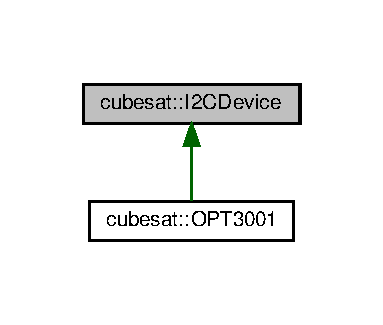
\includegraphics[width=184pt]{classcubesat_1_1I2CDevice__inherit__graph}
\end{center}
\end{figure}
\subsection*{Public Member Functions}
\begin{DoxyCompactItemize}
\item 
\hyperlink{classcubesat_1_1I2CDevice_afa6d28cbaab65cfc2ad60a63bc95d30d}{I2\+C\+Device} ()
\item 
\hyperlink{classcubesat_1_1I2CDevice_a9fad0233c906bdbbe9b66ceaacfbb35e}{I2\+C\+Device} (uint8\+\_\+t \hyperlink{classcubesat_1_1I2CDevice_acc13c6328bb7f29ddc5b9436d6b40816}{bus}, uint8\+\_\+t \hyperlink{classcubesat_1_1I2CDevice_a59cdefbd8b9720d194254c617f5c9b07}{device})
\item 
virtual \hyperlink{classcubesat_1_1I2CDevice_aebf54d150dca31a5bd8ddd524cb5bb00}{$\sim$\+I2\+C\+Device} ()
\item 
virtual int \hyperlink{classcubesat_1_1I2CDevice_a9a3ac852fdca8da83bcf5d771c710264}{Open} ()
\item 
virtual void \hyperlink{classcubesat_1_1I2CDevice_a09c6fe7b6318662e4438ee52c21cee20}{Close} ()
\item 
bool \hyperlink{classcubesat_1_1I2CDevice_abcc65de8ac56247998f20a0023351959}{Is\+Open} () const
\item 
int \hyperlink{classcubesat_1_1I2CDevice_aae688e4c62fafe205028fc0301492b40}{Get\+Bus\+Addr} () const
\item 
int \hyperlink{classcubesat_1_1I2CDevice_a9621077493039877b663245a0491c3fa}{Get\+Device\+Addr} () const
\item 
std\+::string \hyperlink{classcubesat_1_1I2CDevice_aa5919f5bdade4ad2d4ca5b54894350b7}{Get\+Device\+Path} () const
\item 
virtual int \hyperlink{classcubesat_1_1I2CDevice_a4c961bc762deb1388a541f148de32b7e}{Write} (uint8\+\_\+t value)
\item 
virtual int \hyperlink{classcubesat_1_1I2CDevice_ae80e31206a3b08754ca9649326c7e682}{Write\+Register} (uint8\+\_\+t register\+\_\+addr, uint16\+\_\+t value)
\item 
virtual int \hyperlink{classcubesat_1_1I2CDevice_ade46491355547ba50c00a078527dff93}{Read\+Registers} (uint8\+\_\+t $\ast$out, uint8\+\_\+t first\+\_\+addr, uint8\+\_\+t len)
\item 
virtual uint16\+\_\+t \hyperlink{classcubesat_1_1I2CDevice_a398afc2399a0c9164398ee8fdb759669}{Read\+Register} (uint8\+\_\+t register\+\_\+addr)
\end{DoxyCompactItemize}
\subsection*{Private Attributes}
\begin{DoxyCompactItemize}
\item 
int \hyperlink{classcubesat_1_1I2CDevice_acc13c6328bb7f29ddc5b9436d6b40816}{bus}
\item 
int \hyperlink{classcubesat_1_1I2CDevice_a59cdefbd8b9720d194254c617f5c9b07}{device}
\item 
int \hyperlink{classcubesat_1_1I2CDevice_aea3a1fc10a89f78e12f6a905dfa7deb1}{file}
\item 
bool \hyperlink{classcubesat_1_1I2CDevice_a6d247df5f1726283a1783810305c2699}{is\+\_\+open} = false
\end{DoxyCompactItemize}


\subsection{Constructor \& Destructor Documentation}
\mbox{\Hypertarget{classcubesat_1_1I2CDevice_afa6d28cbaab65cfc2ad60a63bc95d30d}\label{classcubesat_1_1I2CDevice_afa6d28cbaab65cfc2ad60a63bc95d30d}} 
\index{cubesat\+::\+I2\+C\+Device@{cubesat\+::\+I2\+C\+Device}!I2\+C\+Device@{I2\+C\+Device}}
\index{I2\+C\+Device@{I2\+C\+Device}!cubesat\+::\+I2\+C\+Device@{cubesat\+::\+I2\+C\+Device}}
\subsubsection{\texorpdfstring{I2\+C\+Device()}{I2CDevice()}\hspace{0.1cm}{\footnotesize\ttfamily [1/2]}}
{\footnotesize\ttfamily I2\+C\+Device\+::\+I2\+C\+Device (\begin{DoxyParamCaption}{ }\end{DoxyParamCaption})}

\mbox{\Hypertarget{classcubesat_1_1I2CDevice_a9fad0233c906bdbbe9b66ceaacfbb35e}\label{classcubesat_1_1I2CDevice_a9fad0233c906bdbbe9b66ceaacfbb35e}} 
\index{cubesat\+::\+I2\+C\+Device@{cubesat\+::\+I2\+C\+Device}!I2\+C\+Device@{I2\+C\+Device}}
\index{I2\+C\+Device@{I2\+C\+Device}!cubesat\+::\+I2\+C\+Device@{cubesat\+::\+I2\+C\+Device}}
\subsubsection{\texorpdfstring{I2\+C\+Device()}{I2CDevice()}\hspace{0.1cm}{\footnotesize\ttfamily [2/2]}}
{\footnotesize\ttfamily I2\+C\+Device\+::\+I2\+C\+Device (\begin{DoxyParamCaption}\item[{uint8\+\_\+t}]{bus,  }\item[{uint8\+\_\+t}]{device }\end{DoxyParamCaption})}

Constructor for the \hyperlink{classcubesat_1_1I2CDevice}{I2\+C\+Device} class. It requires the bus number and device number. The constructor opens a file handle to the I2C device, which is destroyed when the destructor is called 
\begin{DoxyParams}{Parameters}
{\em bus} & The bus number. Usually 0 or 1 on the B\+BB \\
\hline
{\em device} & The device ID on the bus. \\
\hline
\end{DoxyParams}
\mbox{\Hypertarget{classcubesat_1_1I2CDevice_aebf54d150dca31a5bd8ddd524cb5bb00}\label{classcubesat_1_1I2CDevice_aebf54d150dca31a5bd8ddd524cb5bb00}} 
\index{cubesat\+::\+I2\+C\+Device@{cubesat\+::\+I2\+C\+Device}!````~I2\+C\+Device@{$\sim$\+I2\+C\+Device}}
\index{````~I2\+C\+Device@{$\sim$\+I2\+C\+Device}!cubesat\+::\+I2\+C\+Device@{cubesat\+::\+I2\+C\+Device}}
\subsubsection{\texorpdfstring{$\sim$\+I2\+C\+Device()}{~I2CDevice()}}
{\footnotesize\ttfamily I2\+C\+Device\+::$\sim$\+I2\+C\+Device (\begin{DoxyParamCaption}{ }\end{DoxyParamCaption})\hspace{0.3cm}{\ttfamily [virtual]}}

Closes the file on destruction, provided that it has not already been closed. 

\subsection{Member Function Documentation}
\mbox{\Hypertarget{classcubesat_1_1I2CDevice_a09c6fe7b6318662e4438ee52c21cee20}\label{classcubesat_1_1I2CDevice_a09c6fe7b6318662e4438ee52c21cee20}} 
\index{cubesat\+::\+I2\+C\+Device@{cubesat\+::\+I2\+C\+Device}!Close@{Close}}
\index{Close@{Close}!cubesat\+::\+I2\+C\+Device@{cubesat\+::\+I2\+C\+Device}}
\subsubsection{\texorpdfstring{Close()}{Close()}}
{\footnotesize\ttfamily void I2\+C\+Device\+::\+Close (\begin{DoxyParamCaption}{ }\end{DoxyParamCaption})\hspace{0.3cm}{\ttfamily [virtual]}}

Close the file handles and sets a temporary state to -\/1. \mbox{\Hypertarget{classcubesat_1_1I2CDevice_aae688e4c62fafe205028fc0301492b40}\label{classcubesat_1_1I2CDevice_aae688e4c62fafe205028fc0301492b40}} 
\index{cubesat\+::\+I2\+C\+Device@{cubesat\+::\+I2\+C\+Device}!Get\+Bus\+Addr@{Get\+Bus\+Addr}}
\index{Get\+Bus\+Addr@{Get\+Bus\+Addr}!cubesat\+::\+I2\+C\+Device@{cubesat\+::\+I2\+C\+Device}}
\subsubsection{\texorpdfstring{Get\+Bus\+Addr()}{GetBusAddr()}}
{\footnotesize\ttfamily int cubesat\+::\+I2\+C\+Device\+::\+Get\+Bus\+Addr (\begin{DoxyParamCaption}{ }\end{DoxyParamCaption}) const\hspace{0.3cm}{\ttfamily [inline]}}

\mbox{\Hypertarget{classcubesat_1_1I2CDevice_a9621077493039877b663245a0491c3fa}\label{classcubesat_1_1I2CDevice_a9621077493039877b663245a0491c3fa}} 
\index{cubesat\+::\+I2\+C\+Device@{cubesat\+::\+I2\+C\+Device}!Get\+Device\+Addr@{Get\+Device\+Addr}}
\index{Get\+Device\+Addr@{Get\+Device\+Addr}!cubesat\+::\+I2\+C\+Device@{cubesat\+::\+I2\+C\+Device}}
\subsubsection{\texorpdfstring{Get\+Device\+Addr()}{GetDeviceAddr()}}
{\footnotesize\ttfamily int cubesat\+::\+I2\+C\+Device\+::\+Get\+Device\+Addr (\begin{DoxyParamCaption}{ }\end{DoxyParamCaption}) const\hspace{0.3cm}{\ttfamily [inline]}}

\mbox{\Hypertarget{classcubesat_1_1I2CDevice_aa5919f5bdade4ad2d4ca5b54894350b7}\label{classcubesat_1_1I2CDevice_aa5919f5bdade4ad2d4ca5b54894350b7}} 
\index{cubesat\+::\+I2\+C\+Device@{cubesat\+::\+I2\+C\+Device}!Get\+Device\+Path@{Get\+Device\+Path}}
\index{Get\+Device\+Path@{Get\+Device\+Path}!cubesat\+::\+I2\+C\+Device@{cubesat\+::\+I2\+C\+Device}}
\subsubsection{\texorpdfstring{Get\+Device\+Path()}{GetDevicePath()}}
{\footnotesize\ttfamily std\+::string I2\+C\+Device\+::\+Get\+Device\+Path (\begin{DoxyParamCaption}{ }\end{DoxyParamCaption}) const}

\mbox{\Hypertarget{classcubesat_1_1I2CDevice_abcc65de8ac56247998f20a0023351959}\label{classcubesat_1_1I2CDevice_abcc65de8ac56247998f20a0023351959}} 
\index{cubesat\+::\+I2\+C\+Device@{cubesat\+::\+I2\+C\+Device}!Is\+Open@{Is\+Open}}
\index{Is\+Open@{Is\+Open}!cubesat\+::\+I2\+C\+Device@{cubesat\+::\+I2\+C\+Device}}
\subsubsection{\texorpdfstring{Is\+Open()}{IsOpen()}}
{\footnotesize\ttfamily bool cubesat\+::\+I2\+C\+Device\+::\+Is\+Open (\begin{DoxyParamCaption}{ }\end{DoxyParamCaption}) const\hspace{0.3cm}{\ttfamily [inline]}}

\mbox{\Hypertarget{classcubesat_1_1I2CDevice_a9a3ac852fdca8da83bcf5d771c710264}\label{classcubesat_1_1I2CDevice_a9a3ac852fdca8da83bcf5d771c710264}} 
\index{cubesat\+::\+I2\+C\+Device@{cubesat\+::\+I2\+C\+Device}!Open@{Open}}
\index{Open@{Open}!cubesat\+::\+I2\+C\+Device@{cubesat\+::\+I2\+C\+Device}}
\subsubsection{\texorpdfstring{Open()}{Open()}}
{\footnotesize\ttfamily int I2\+C\+Device\+::\+Open (\begin{DoxyParamCaption}{ }\end{DoxyParamCaption})\hspace{0.3cm}{\ttfamily [virtual]}}

Open a connection to an I2C device \begin{DoxyReturn}{Returns}
-\/1 on failure to open to the bus or device, 0 on success. 
\end{DoxyReturn}
\mbox{\Hypertarget{classcubesat_1_1I2CDevice_a398afc2399a0c9164398ee8fdb759669}\label{classcubesat_1_1I2CDevice_a398afc2399a0c9164398ee8fdb759669}} 
\index{cubesat\+::\+I2\+C\+Device@{cubesat\+::\+I2\+C\+Device}!Read\+Register@{Read\+Register}}
\index{Read\+Register@{Read\+Register}!cubesat\+::\+I2\+C\+Device@{cubesat\+::\+I2\+C\+Device}}
\subsubsection{\texorpdfstring{Read\+Register()}{ReadRegister()}}
{\footnotesize\ttfamily uint16\+\_\+t I2\+C\+Device\+::\+Read\+Register (\begin{DoxyParamCaption}\item[{uint8\+\_\+t}]{register\+Address }\end{DoxyParamCaption})\hspace{0.3cm}{\ttfamily [virtual]}}

Read a single register value from the address on the device. 
\begin{DoxyParams}{Parameters}
{\em register\+Address} & the address to read from \\
\hline
\end{DoxyParams}
\begin{DoxyReturn}{Returns}
the byte value at the register address. 
\end{DoxyReturn}
\mbox{\Hypertarget{classcubesat_1_1I2CDevice_ade46491355547ba50c00a078527dff93}\label{classcubesat_1_1I2CDevice_ade46491355547ba50c00a078527dff93}} 
\index{cubesat\+::\+I2\+C\+Device@{cubesat\+::\+I2\+C\+Device}!Read\+Registers@{Read\+Registers}}
\index{Read\+Registers@{Read\+Registers}!cubesat\+::\+I2\+C\+Device@{cubesat\+::\+I2\+C\+Device}}
\subsubsection{\texorpdfstring{Read\+Registers()}{ReadRegisters()}}
{\footnotesize\ttfamily int I2\+C\+Device\+::\+Read\+Registers (\begin{DoxyParamCaption}\item[{uint8\+\_\+t $\ast$}]{out,  }\item[{uint8\+\_\+t}]{first\+\_\+addr,  }\item[{uint8\+\_\+t}]{len }\end{DoxyParamCaption})\hspace{0.3cm}{\ttfamily [virtual]}}

Method to read a number of registers from a single device. This is much more efficient than reading the registers individually. The from address is the starting address to read from, which defaults to 0x00. 
\begin{DoxyParams}{Parameters}
{\em number} & the number of registers to read from the device \\
\hline
{\em from\+Address} & the starting address to read from \\
\hline
\end{DoxyParams}
\begin{DoxyReturn}{Returns}
a pointer of type unsigned char$\ast$ that points to the first element in the block of registers 
\end{DoxyReturn}
\mbox{\Hypertarget{classcubesat_1_1I2CDevice_a4c961bc762deb1388a541f148de32b7e}\label{classcubesat_1_1I2CDevice_a4c961bc762deb1388a541f148de32b7e}} 
\index{cubesat\+::\+I2\+C\+Device@{cubesat\+::\+I2\+C\+Device}!Write@{Write}}
\index{Write@{Write}!cubesat\+::\+I2\+C\+Device@{cubesat\+::\+I2\+C\+Device}}
\subsubsection{\texorpdfstring{Write()}{Write()}}
{\footnotesize\ttfamily int I2\+C\+Device\+::\+Write (\begin{DoxyParamCaption}\item[{uint8\+\_\+t}]{value }\end{DoxyParamCaption})\hspace{0.3cm}{\ttfamily [virtual]}}

Write a single value to the I2C device. Used to set up the device to read from a particular address. 
\begin{DoxyParams}{Parameters}
{\em value} & the value to write to the device \\
\hline
\end{DoxyParams}
\begin{DoxyReturn}{Returns}
-\/1 on failure to write, 0 on success. 
\end{DoxyReturn}
\mbox{\Hypertarget{classcubesat_1_1I2CDevice_ae80e31206a3b08754ca9649326c7e682}\label{classcubesat_1_1I2CDevice_ae80e31206a3b08754ca9649326c7e682}} 
\index{cubesat\+::\+I2\+C\+Device@{cubesat\+::\+I2\+C\+Device}!Write\+Register@{Write\+Register}}
\index{Write\+Register@{Write\+Register}!cubesat\+::\+I2\+C\+Device@{cubesat\+::\+I2\+C\+Device}}
\subsubsection{\texorpdfstring{Write\+Register()}{WriteRegister()}}
{\footnotesize\ttfamily int I2\+C\+Device\+::\+Write\+Register (\begin{DoxyParamCaption}\item[{uint8\+\_\+t}]{register\+Address,  }\item[{uint16\+\_\+t}]{value }\end{DoxyParamCaption})\hspace{0.3cm}{\ttfamily [virtual]}}

Write a single byte value to a single register. 
\begin{DoxyParams}{Parameters}
{\em register\+Address} & The register address \\
\hline
{\em value} & The value to be written to the register \\
\hline
\end{DoxyParams}
\begin{DoxyReturn}{Returns}
-\/1 on failure to write, 0 on success. 
\end{DoxyReturn}


\subsection{Member Data Documentation}
\mbox{\Hypertarget{classcubesat_1_1I2CDevice_acc13c6328bb7f29ddc5b9436d6b40816}\label{classcubesat_1_1I2CDevice_acc13c6328bb7f29ddc5b9436d6b40816}} 
\index{cubesat\+::\+I2\+C\+Device@{cubesat\+::\+I2\+C\+Device}!bus@{bus}}
\index{bus@{bus}!cubesat\+::\+I2\+C\+Device@{cubesat\+::\+I2\+C\+Device}}
\subsubsection{\texorpdfstring{bus}{bus}}
{\footnotesize\ttfamily int cubesat\+::\+I2\+C\+Device\+::bus\hspace{0.3cm}{\ttfamily [private]}}

\mbox{\Hypertarget{classcubesat_1_1I2CDevice_a59cdefbd8b9720d194254c617f5c9b07}\label{classcubesat_1_1I2CDevice_a59cdefbd8b9720d194254c617f5c9b07}} 
\index{cubesat\+::\+I2\+C\+Device@{cubesat\+::\+I2\+C\+Device}!device@{device}}
\index{device@{device}!cubesat\+::\+I2\+C\+Device@{cubesat\+::\+I2\+C\+Device}}
\subsubsection{\texorpdfstring{device}{device}}
{\footnotesize\ttfamily int cubesat\+::\+I2\+C\+Device\+::device\hspace{0.3cm}{\ttfamily [private]}}

\mbox{\Hypertarget{classcubesat_1_1I2CDevice_aea3a1fc10a89f78e12f6a905dfa7deb1}\label{classcubesat_1_1I2CDevice_aea3a1fc10a89f78e12f6a905dfa7deb1}} 
\index{cubesat\+::\+I2\+C\+Device@{cubesat\+::\+I2\+C\+Device}!file@{file}}
\index{file@{file}!cubesat\+::\+I2\+C\+Device@{cubesat\+::\+I2\+C\+Device}}
\subsubsection{\texorpdfstring{file}{file}}
{\footnotesize\ttfamily int cubesat\+::\+I2\+C\+Device\+::file\hspace{0.3cm}{\ttfamily [private]}}

\mbox{\Hypertarget{classcubesat_1_1I2CDevice_a6d247df5f1726283a1783810305c2699}\label{classcubesat_1_1I2CDevice_a6d247df5f1726283a1783810305c2699}} 
\index{cubesat\+::\+I2\+C\+Device@{cubesat\+::\+I2\+C\+Device}!is\+\_\+open@{is\+\_\+open}}
\index{is\+\_\+open@{is\+\_\+open}!cubesat\+::\+I2\+C\+Device@{cubesat\+::\+I2\+C\+Device}}
\subsubsection{\texorpdfstring{is\+\_\+open}{is\_open}}
{\footnotesize\ttfamily bool cubesat\+::\+I2\+C\+Device\+::is\+\_\+open = false\hspace{0.3cm}{\ttfamily [private]}}



The documentation for this class was generated from the following files\+:\begin{DoxyCompactItemize}
\item 
/home/osboxes/cosmos/source/projects/cubesat-\/kit/include/device/\hyperlink{I2CDevice_8h}{I2\+C\+Device.\+h}\item 
/home/osboxes/cosmos/source/projects/cubesat-\/kit/source/device/\hyperlink{I2CDevice_8cpp}{I2\+C\+Device.\+cpp}\end{DoxyCompactItemize}

\hypertarget{classcubesat_1_1IMU}{}\section{cubesat\+:\+:I\+MU Class Reference}
\label{classcubesat_1_1IMU}\index{cubesat\+::\+I\+MU@{cubesat\+::\+I\+MU}}


{\ttfamily \#include $<$Device.\+h$>$}



Inheritance diagram for cubesat\+:\+:I\+MU\+:
\nopagebreak
\begin{figure}[H]
\begin{center}
\leavevmode
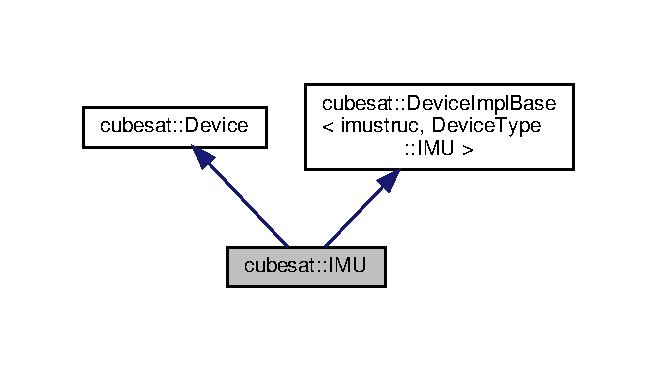
\includegraphics[width=316pt]{classcubesat_1_1IMU__inherit__graph}
\end{center}
\end{figure}


Collaboration diagram for cubesat\+:\+:I\+MU\+:
\nopagebreak
\begin{figure}[H]
\begin{center}
\leavevmode
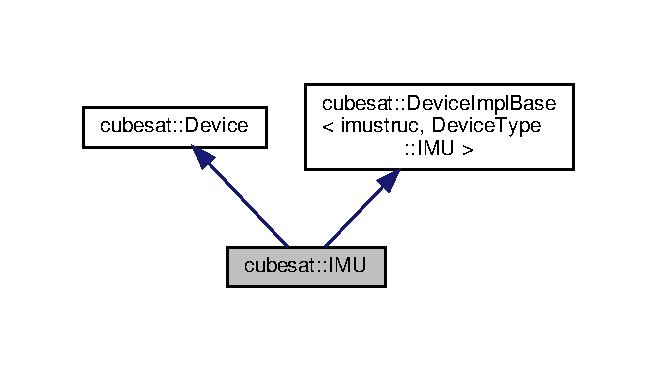
\includegraphics[width=316pt]{classcubesat_1_1IMU__coll__graph}
\end{center}
\end{figure}
\subsection*{Public Member Functions}
\begin{DoxyCompactItemize}
\item 
\hyperlink{classcubesat_1_1IMU_a1064c287bc98ce3d4042c1a08b59ca2b}{I\+MU} (Agent $\ast$\hyperlink{classcubesat_1_1Device_a8499108eccaf7375bea8ead0182391a6}{agent}, int \hyperlink{classcubesat_1_1Device_a1deca725b01f8ef37e49662da6db4e53}{cindex}, int \hyperlink{classcubesat_1_1Device_a8a2b3d6d7400e6796c31705058172982}{dindex})
\item 
virtual \hyperlink{classcubesat_1_1IMU_af9587ba377181ff65d9a3ef5bc19bb24}{$\sim$\+I\+MU} ()
\item 
\hyperlink{classcubesat_1_1IMU_ac48481fb52ed8c9155ccea48484738a2}{\+\_\+\+Add\+Property} (temperature, temp)
\item 
\hyperlink{classcubesat_1_1IMU_af384f6d5ac565eeb51c5f8ec50773845}{\+\_\+\+Add\+Property} (utc, utc)
\item 
\hyperlink{classcubesat_1_1IMU_a9b5f473c643c654fa963aa756296e186}{\+\_\+\+Add\+Property} (voltage, volt)
\item 
\hyperlink{classcubesat_1_1IMU_ab6d6a9261f4c761ffead00a40ffd731f}{\+\_\+\+Add\+Property} (current, amp)
\item 
\hyperlink{classcubesat_1_1IMU_ad3eaf019d8e56033e3a9a4a94775f814}{\+\_\+\+Add\+Property} (power, power)
\item 
\hyperlink{classcubesat_1_1IMU_ae66574a8d8e15c58e3ccd8193e59adea}{\+\_\+\+Add\+Property} (enabled, enabled)
\item 
\hyperlink{classcubesat_1_1IMU_aa6aeefd6704b05dfd59ca1476099aed7}{\+\_\+\+Add\+Property} (magnetic\+\_\+field, mag)
\item 
\hyperlink{classcubesat_1_1IMU_aedeb160bf398d47205b0206f1ee96fb7}{\+\_\+\+Add\+Property} (acceleration, accel)
\item 
\hyperlink{classcubesat_1_1IMU_aace8a3f33f5c953bbdd456ccf77c9d8a}{\+\_\+\+Add\+Property} (angular\+\_\+velocity, omega)
\end{DoxyCompactItemize}
\subsection*{Additional Inherited Members}


\subsection{Constructor \& Destructor Documentation}
\mbox{\Hypertarget{classcubesat_1_1IMU_a1064c287bc98ce3d4042c1a08b59ca2b}\label{classcubesat_1_1IMU_a1064c287bc98ce3d4042c1a08b59ca2b}} 
\index{cubesat\+::\+I\+MU@{cubesat\+::\+I\+MU}!I\+MU@{I\+MU}}
\index{I\+MU@{I\+MU}!cubesat\+::\+I\+MU@{cubesat\+::\+I\+MU}}
\subsubsection{\texorpdfstring{I\+M\+U()}{IMU()}}
{\footnotesize\ttfamily cubesat\+::\+I\+M\+U\+::\+I\+MU (\begin{DoxyParamCaption}\item[{Agent $\ast$}]{agent,  }\item[{int}]{cindex,  }\item[{int}]{dindex }\end{DoxyParamCaption})\hspace{0.3cm}{\ttfamily [inline]}}

\mbox{\Hypertarget{classcubesat_1_1IMU_af9587ba377181ff65d9a3ef5bc19bb24}\label{classcubesat_1_1IMU_af9587ba377181ff65d9a3ef5bc19bb24}} 
\index{cubesat\+::\+I\+MU@{cubesat\+::\+I\+MU}!````~I\+MU@{$\sim$\+I\+MU}}
\index{````~I\+MU@{$\sim$\+I\+MU}!cubesat\+::\+I\+MU@{cubesat\+::\+I\+MU}}
\subsubsection{\texorpdfstring{$\sim$\+I\+M\+U()}{~IMU()}}
{\footnotesize\ttfamily virtual cubesat\+::\+I\+M\+U\+::$\sim$\+I\+MU (\begin{DoxyParamCaption}{ }\end{DoxyParamCaption})\hspace{0.3cm}{\ttfamily [inline]}, {\ttfamily [virtual]}}



\subsection{Member Function Documentation}
\mbox{\Hypertarget{classcubesat_1_1IMU_ac48481fb52ed8c9155ccea48484738a2}\label{classcubesat_1_1IMU_ac48481fb52ed8c9155ccea48484738a2}} 
\index{cubesat\+::\+I\+MU@{cubesat\+::\+I\+MU}!\+\_\+\+Add\+Property@{\+\_\+\+Add\+Property}}
\index{\+\_\+\+Add\+Property@{\+\_\+\+Add\+Property}!cubesat\+::\+I\+MU@{cubesat\+::\+I\+MU}}
\subsubsection{\texorpdfstring{\+\_\+\+Add\+Property()}{\_AddProperty()}\hspace{0.1cm}{\footnotesize\ttfamily [1/9]}}
{\footnotesize\ttfamily cubesat\+::\+I\+M\+U\+::\+\_\+\+Add\+Property (\begin{DoxyParamCaption}\item[{temperature}]{,  }\item[{temp}]{ }\end{DoxyParamCaption})}

\mbox{\Hypertarget{classcubesat_1_1IMU_af384f6d5ac565eeb51c5f8ec50773845}\label{classcubesat_1_1IMU_af384f6d5ac565eeb51c5f8ec50773845}} 
\index{cubesat\+::\+I\+MU@{cubesat\+::\+I\+MU}!\+\_\+\+Add\+Property@{\+\_\+\+Add\+Property}}
\index{\+\_\+\+Add\+Property@{\+\_\+\+Add\+Property}!cubesat\+::\+I\+MU@{cubesat\+::\+I\+MU}}
\subsubsection{\texorpdfstring{\+\_\+\+Add\+Property()}{\_AddProperty()}\hspace{0.1cm}{\footnotesize\ttfamily [2/9]}}
{\footnotesize\ttfamily cubesat\+::\+I\+M\+U\+::\+\_\+\+Add\+Property (\begin{DoxyParamCaption}\item[{utc}]{,  }\item[{utc}]{ }\end{DoxyParamCaption})}

\mbox{\Hypertarget{classcubesat_1_1IMU_a9b5f473c643c654fa963aa756296e186}\label{classcubesat_1_1IMU_a9b5f473c643c654fa963aa756296e186}} 
\index{cubesat\+::\+I\+MU@{cubesat\+::\+I\+MU}!\+\_\+\+Add\+Property@{\+\_\+\+Add\+Property}}
\index{\+\_\+\+Add\+Property@{\+\_\+\+Add\+Property}!cubesat\+::\+I\+MU@{cubesat\+::\+I\+MU}}
\subsubsection{\texorpdfstring{\+\_\+\+Add\+Property()}{\_AddProperty()}\hspace{0.1cm}{\footnotesize\ttfamily [3/9]}}
{\footnotesize\ttfamily cubesat\+::\+I\+M\+U\+::\+\_\+\+Add\+Property (\begin{DoxyParamCaption}\item[{voltage}]{,  }\item[{volt}]{ }\end{DoxyParamCaption})}

\mbox{\Hypertarget{classcubesat_1_1IMU_ab6d6a9261f4c761ffead00a40ffd731f}\label{classcubesat_1_1IMU_ab6d6a9261f4c761ffead00a40ffd731f}} 
\index{cubesat\+::\+I\+MU@{cubesat\+::\+I\+MU}!\+\_\+\+Add\+Property@{\+\_\+\+Add\+Property}}
\index{\+\_\+\+Add\+Property@{\+\_\+\+Add\+Property}!cubesat\+::\+I\+MU@{cubesat\+::\+I\+MU}}
\subsubsection{\texorpdfstring{\+\_\+\+Add\+Property()}{\_AddProperty()}\hspace{0.1cm}{\footnotesize\ttfamily [4/9]}}
{\footnotesize\ttfamily cubesat\+::\+I\+M\+U\+::\+\_\+\+Add\+Property (\begin{DoxyParamCaption}\item[{current}]{,  }\item[{amp}]{ }\end{DoxyParamCaption})}

\mbox{\Hypertarget{classcubesat_1_1IMU_ad3eaf019d8e56033e3a9a4a94775f814}\label{classcubesat_1_1IMU_ad3eaf019d8e56033e3a9a4a94775f814}} 
\index{cubesat\+::\+I\+MU@{cubesat\+::\+I\+MU}!\+\_\+\+Add\+Property@{\+\_\+\+Add\+Property}}
\index{\+\_\+\+Add\+Property@{\+\_\+\+Add\+Property}!cubesat\+::\+I\+MU@{cubesat\+::\+I\+MU}}
\subsubsection{\texorpdfstring{\+\_\+\+Add\+Property()}{\_AddProperty()}\hspace{0.1cm}{\footnotesize\ttfamily [5/9]}}
{\footnotesize\ttfamily cubesat\+::\+I\+M\+U\+::\+\_\+\+Add\+Property (\begin{DoxyParamCaption}\item[{power}]{,  }\item[{power}]{ }\end{DoxyParamCaption})}

\mbox{\Hypertarget{classcubesat_1_1IMU_ae66574a8d8e15c58e3ccd8193e59adea}\label{classcubesat_1_1IMU_ae66574a8d8e15c58e3ccd8193e59adea}} 
\index{cubesat\+::\+I\+MU@{cubesat\+::\+I\+MU}!\+\_\+\+Add\+Property@{\+\_\+\+Add\+Property}}
\index{\+\_\+\+Add\+Property@{\+\_\+\+Add\+Property}!cubesat\+::\+I\+MU@{cubesat\+::\+I\+MU}}
\subsubsection{\texorpdfstring{\+\_\+\+Add\+Property()}{\_AddProperty()}\hspace{0.1cm}{\footnotesize\ttfamily [6/9]}}
{\footnotesize\ttfamily cubesat\+::\+I\+M\+U\+::\+\_\+\+Add\+Property (\begin{DoxyParamCaption}\item[{enabled}]{,  }\item[{enabled}]{ }\end{DoxyParamCaption})}

\mbox{\Hypertarget{classcubesat_1_1IMU_aa6aeefd6704b05dfd59ca1476099aed7}\label{classcubesat_1_1IMU_aa6aeefd6704b05dfd59ca1476099aed7}} 
\index{cubesat\+::\+I\+MU@{cubesat\+::\+I\+MU}!\+\_\+\+Add\+Property@{\+\_\+\+Add\+Property}}
\index{\+\_\+\+Add\+Property@{\+\_\+\+Add\+Property}!cubesat\+::\+I\+MU@{cubesat\+::\+I\+MU}}
\subsubsection{\texorpdfstring{\+\_\+\+Add\+Property()}{\_AddProperty()}\hspace{0.1cm}{\footnotesize\ttfamily [7/9]}}
{\footnotesize\ttfamily cubesat\+::\+I\+M\+U\+::\+\_\+\+Add\+Property (\begin{DoxyParamCaption}\item[{magnetic\+\_\+field}]{,  }\item[{mag}]{ }\end{DoxyParamCaption})}

\mbox{\Hypertarget{classcubesat_1_1IMU_aedeb160bf398d47205b0206f1ee96fb7}\label{classcubesat_1_1IMU_aedeb160bf398d47205b0206f1ee96fb7}} 
\index{cubesat\+::\+I\+MU@{cubesat\+::\+I\+MU}!\+\_\+\+Add\+Property@{\+\_\+\+Add\+Property}}
\index{\+\_\+\+Add\+Property@{\+\_\+\+Add\+Property}!cubesat\+::\+I\+MU@{cubesat\+::\+I\+MU}}
\subsubsection{\texorpdfstring{\+\_\+\+Add\+Property()}{\_AddProperty()}\hspace{0.1cm}{\footnotesize\ttfamily [8/9]}}
{\footnotesize\ttfamily cubesat\+::\+I\+M\+U\+::\+\_\+\+Add\+Property (\begin{DoxyParamCaption}\item[{acceleration}]{,  }\item[{accel}]{ }\end{DoxyParamCaption})}

\mbox{\Hypertarget{classcubesat_1_1IMU_aace8a3f33f5c953bbdd456ccf77c9d8a}\label{classcubesat_1_1IMU_aace8a3f33f5c953bbdd456ccf77c9d8a}} 
\index{cubesat\+::\+I\+MU@{cubesat\+::\+I\+MU}!\+\_\+\+Add\+Property@{\+\_\+\+Add\+Property}}
\index{\+\_\+\+Add\+Property@{\+\_\+\+Add\+Property}!cubesat\+::\+I\+MU@{cubesat\+::\+I\+MU}}
\subsubsection{\texorpdfstring{\+\_\+\+Add\+Property()}{\_AddProperty()}\hspace{0.1cm}{\footnotesize\ttfamily [9/9]}}
{\footnotesize\ttfamily cubesat\+::\+I\+M\+U\+::\+\_\+\+Add\+Property (\begin{DoxyParamCaption}\item[{angular\+\_\+velocity}]{,  }\item[{omega}]{ }\end{DoxyParamCaption})}



The documentation for this class was generated from the following file\+:\begin{DoxyCompactItemize}
\item 
/home/osboxes/cosmos/source/projects/cubesat-\/kit/include/utility/\hyperlink{Device_8h}{Device.\+h}\end{DoxyCompactItemize}

\hypertarget{classcubesat_1_1KHLVA0504}{}\section{cubesat\+:\+:K\+H\+L\+V\+A0504 Class Reference}
\label{classcubesat_1_1KHLVA0504}\index{cubesat\+::\+K\+H\+L\+V\+A0504@{cubesat\+::\+K\+H\+L\+V\+A0504}}


{\ttfamily \#include $<$K\+H\+L\+V\+A0504.\+h$>$}

\subsection*{Public Member Functions}
\begin{DoxyCompactItemize}
\item 
void \hyperlink{classcubesat_1_1KHLVA0504_a6aa41de16a51df29cf4ba99cf6533bba}{Enable} ()
\item 
void \hyperlink{classcubesat_1_1KHLVA0504_aa9ca7967617d398e01c07b6d00d1f7fe}{Disable} ()
\end{DoxyCompactItemize}


\subsection{Member Function Documentation}
\mbox{\Hypertarget{classcubesat_1_1KHLVA0504_aa9ca7967617d398e01c07b6d00d1f7fe}\label{classcubesat_1_1KHLVA0504_aa9ca7967617d398e01c07b6d00d1f7fe}} 
\index{cubesat\+::\+K\+H\+L\+V\+A0504@{cubesat\+::\+K\+H\+L\+V\+A0504}!Disable@{Disable}}
\index{Disable@{Disable}!cubesat\+::\+K\+H\+L\+V\+A0504@{cubesat\+::\+K\+H\+L\+V\+A0504}}
\subsubsection{\texorpdfstring{Disable()}{Disable()}}
{\footnotesize\ttfamily void cubesat\+::\+K\+H\+L\+V\+A0504\+::\+Disable (\begin{DoxyParamCaption}{ }\end{DoxyParamCaption})}

\mbox{\Hypertarget{classcubesat_1_1KHLVA0504_a6aa41de16a51df29cf4ba99cf6533bba}\label{classcubesat_1_1KHLVA0504_a6aa41de16a51df29cf4ba99cf6533bba}} 
\index{cubesat\+::\+K\+H\+L\+V\+A0504@{cubesat\+::\+K\+H\+L\+V\+A0504}!Enable@{Enable}}
\index{Enable@{Enable}!cubesat\+::\+K\+H\+L\+V\+A0504@{cubesat\+::\+K\+H\+L\+V\+A0504}}
\subsubsection{\texorpdfstring{Enable()}{Enable()}}
{\footnotesize\ttfamily void cubesat\+::\+K\+H\+L\+V\+A0504\+::\+Enable (\begin{DoxyParamCaption}{ }\end{DoxyParamCaption})}



The documentation for this class was generated from the following file\+:\begin{DoxyCompactItemize}
\item 
/home/osboxes/cosmos/source/projects/cubesat-\/kit/include/device/\hyperlink{KHLVA0504_8h}{K\+H\+L\+V\+A0504.\+h}\end{DoxyCompactItemize}

\hypertarget{structcubesat_1_1Location}{}\section{cubesat\+:\+:Location Struct Reference}
\label{structcubesat_1_1Location}\index{cubesat\+::\+Location@{cubesat\+::\+Location}}


{\ttfamily \#include $<$Types.\+h$>$}

\subsection*{Public Member Functions}
\begin{DoxyCompactItemize}
\item 
\hyperlink{structcubesat_1_1Location_a9de50e8e989fed1771825ff03e53a3a9}{Location} ()
\item 
\hyperlink{structcubesat_1_1Location_a5bb8201f3d6b276e19b4767fd9bfc7dd}{Location} (double \hyperlink{structcubesat_1_1Location_af14b920a59e1ac2ebdb613e46010fd7e}{latitude}, double \hyperlink{structcubesat_1_1Location_a52b9b8a55bdc7c4c8841e331b2bf981a}{longitude}, double \hyperlink{structcubesat_1_1Location_af010a12e2d638d3a47f2cad83811d95a}{altitude})
\item 
\hyperlink{structcubesat_1_1Location_ac6e05f08da64e8dad865013bcbc27223}{Location} (const gvector \&vec)
\item 
\hyperlink{structcubesat_1_1Location_aeeb4a12c93c721cec692882710cc0823}{operator gvector} () const
\end{DoxyCompactItemize}
\subsection*{Public Attributes}
\begin{DoxyCompactItemize}
\item 
double \hyperlink{structcubesat_1_1Location_af14b920a59e1ac2ebdb613e46010fd7e}{latitude}
\item 
double \hyperlink{structcubesat_1_1Location_a52b9b8a55bdc7c4c8841e331b2bf981a}{longitude}
\item 
double \hyperlink{structcubesat_1_1Location_af010a12e2d638d3a47f2cad83811d95a}{altitude}
\end{DoxyCompactItemize}


\subsection{Constructor \& Destructor Documentation}
\mbox{\Hypertarget{structcubesat_1_1Location_a9de50e8e989fed1771825ff03e53a3a9}\label{structcubesat_1_1Location_a9de50e8e989fed1771825ff03e53a3a9}} 
\index{cubesat\+::\+Location@{cubesat\+::\+Location}!Location@{Location}}
\index{Location@{Location}!cubesat\+::\+Location@{cubesat\+::\+Location}}
\subsubsection{\texorpdfstring{Location()}{Location()}\hspace{0.1cm}{\footnotesize\ttfamily [1/3]}}
{\footnotesize\ttfamily cubesat\+::\+Location\+::\+Location (\begin{DoxyParamCaption}{ }\end{DoxyParamCaption})\hspace{0.3cm}{\ttfamily [inline]}}

\mbox{\Hypertarget{structcubesat_1_1Location_a5bb8201f3d6b276e19b4767fd9bfc7dd}\label{structcubesat_1_1Location_a5bb8201f3d6b276e19b4767fd9bfc7dd}} 
\index{cubesat\+::\+Location@{cubesat\+::\+Location}!Location@{Location}}
\index{Location@{Location}!cubesat\+::\+Location@{cubesat\+::\+Location}}
\subsubsection{\texorpdfstring{Location()}{Location()}\hspace{0.1cm}{\footnotesize\ttfamily [2/3]}}
{\footnotesize\ttfamily cubesat\+::\+Location\+::\+Location (\begin{DoxyParamCaption}\item[{double}]{latitude,  }\item[{double}]{longitude,  }\item[{double}]{altitude }\end{DoxyParamCaption})\hspace{0.3cm}{\ttfamily [inline]}}

\mbox{\Hypertarget{structcubesat_1_1Location_ac6e05f08da64e8dad865013bcbc27223}\label{structcubesat_1_1Location_ac6e05f08da64e8dad865013bcbc27223}} 
\index{cubesat\+::\+Location@{cubesat\+::\+Location}!Location@{Location}}
\index{Location@{Location}!cubesat\+::\+Location@{cubesat\+::\+Location}}
\subsubsection{\texorpdfstring{Location()}{Location()}\hspace{0.1cm}{\footnotesize\ttfamily [3/3]}}
{\footnotesize\ttfamily cubesat\+::\+Location\+::\+Location (\begin{DoxyParamCaption}\item[{const gvector \&}]{vec }\end{DoxyParamCaption})\hspace{0.3cm}{\ttfamily [inline]}}



\subsection{Member Function Documentation}
\mbox{\Hypertarget{structcubesat_1_1Location_aeeb4a12c93c721cec692882710cc0823}\label{structcubesat_1_1Location_aeeb4a12c93c721cec692882710cc0823}} 
\index{cubesat\+::\+Location@{cubesat\+::\+Location}!operator gvector@{operator gvector}}
\index{operator gvector@{operator gvector}!cubesat\+::\+Location@{cubesat\+::\+Location}}
\subsubsection{\texorpdfstring{operator gvector()}{operator gvector()}}
{\footnotesize\ttfamily cubesat\+::\+Location\+::operator gvector (\begin{DoxyParamCaption}{ }\end{DoxyParamCaption}) const\hspace{0.3cm}{\ttfamily [inline]}}



\subsection{Member Data Documentation}
\mbox{\Hypertarget{structcubesat_1_1Location_af010a12e2d638d3a47f2cad83811d95a}\label{structcubesat_1_1Location_af010a12e2d638d3a47f2cad83811d95a}} 
\index{cubesat\+::\+Location@{cubesat\+::\+Location}!altitude@{altitude}}
\index{altitude@{altitude}!cubesat\+::\+Location@{cubesat\+::\+Location}}
\subsubsection{\texorpdfstring{altitude}{altitude}}
{\footnotesize\ttfamily double cubesat\+::\+Location\+::altitude}

\mbox{\Hypertarget{structcubesat_1_1Location_af14b920a59e1ac2ebdb613e46010fd7e}\label{structcubesat_1_1Location_af14b920a59e1ac2ebdb613e46010fd7e}} 
\index{cubesat\+::\+Location@{cubesat\+::\+Location}!latitude@{latitude}}
\index{latitude@{latitude}!cubesat\+::\+Location@{cubesat\+::\+Location}}
\subsubsection{\texorpdfstring{latitude}{latitude}}
{\footnotesize\ttfamily double cubesat\+::\+Location\+::latitude}

\mbox{\Hypertarget{structcubesat_1_1Location_a52b9b8a55bdc7c4c8841e331b2bf981a}\label{structcubesat_1_1Location_a52b9b8a55bdc7c4c8841e331b2bf981a}} 
\index{cubesat\+::\+Location@{cubesat\+::\+Location}!longitude@{longitude}}
\index{longitude@{longitude}!cubesat\+::\+Location@{cubesat\+::\+Location}}
\subsubsection{\texorpdfstring{longitude}{longitude}}
{\footnotesize\ttfamily double cubesat\+::\+Location\+::longitude}



The documentation for this struct was generated from the following file\+:\begin{DoxyCompactItemize}
\item 
/home/osboxes/cosmos/source/projects/cubesat-\/kit/include/utility/\hyperlink{Types_8h}{Types.\+h}\end{DoxyCompactItemize}

\hypertarget{unioncubesat_1_1ADT7311_1_1ManufacturerData}{}\section{cubesat\+:\+:A\+D\+T7311\+:\+:Manufacturer\+Data Union Reference}
\label{unioncubesat_1_1ADT7311_1_1ManufacturerData}\index{cubesat\+::\+A\+D\+T7311\+::\+Manufacturer\+Data@{cubesat\+::\+A\+D\+T7311\+::\+Manufacturer\+Data}}


Stores data from the Manufacturer ID register.  




{\ttfamily \#include $<$A\+D\+T7311.\+h$>$}

\subsection*{Public Attributes}
\begin{DoxyCompactItemize}
\item 
uint8\+\_\+t \hyperlink{unioncubesat_1_1ADT7311_1_1ManufacturerData_a020fb0b501cad0bf19424a65654fde11}{raw\+\_\+data}
\item 
\begin{tabbing}
xx\=xx\=xx\=xx\=xx\=xx\=xx\=xx\=xx\=\kill
struct \{\\
\>uint8\_t \hyperlink{unioncubesat_1_1ADT7311_1_1ManufacturerData_a7558c7378e095c03e018e0d2c23d6b16}{revision\_id}: 3\\
\>uint8\_t \hyperlink{unioncubesat_1_1ADT7311_1_1ManufacturerData_a3c8ac9331622f2950347f8a271f55090}{manufacturer\_id}: 5\\
\}; \\

\end{tabbing}\end{DoxyCompactItemize}


\subsection{Detailed Description}
Stores data from the Manufacturer ID register. 

\subsection{Member Data Documentation}
\mbox{\Hypertarget{unioncubesat_1_1ADT7311_1_1ManufacturerData_a96d2d46f618cbad947f2286568fa4a7d}\label{unioncubesat_1_1ADT7311_1_1ManufacturerData_a96d2d46f618cbad947f2286568fa4a7d}} 
\subsubsection{\texorpdfstring{"@7}{@7}}
{\footnotesize\ttfamily struct \{ ... \} }

\mbox{\Hypertarget{unioncubesat_1_1ADT7311_1_1ManufacturerData_a3c8ac9331622f2950347f8a271f55090}\label{unioncubesat_1_1ADT7311_1_1ManufacturerData_a3c8ac9331622f2950347f8a271f55090}} 
\index{cubesat\+::\+A\+D\+T7311\+::\+Manufacturer\+Data@{cubesat\+::\+A\+D\+T7311\+::\+Manufacturer\+Data}!manufacturer\+\_\+id@{manufacturer\+\_\+id}}
\index{manufacturer\+\_\+id@{manufacturer\+\_\+id}!cubesat\+::\+A\+D\+T7311\+::\+Manufacturer\+Data@{cubesat\+::\+A\+D\+T7311\+::\+Manufacturer\+Data}}
\subsubsection{\texorpdfstring{manufacturer\+\_\+id}{manufacturer\_id}}
{\footnotesize\ttfamily uint8\+\_\+t cubesat\+::\+A\+D\+T7311\+::\+Manufacturer\+Data\+::manufacturer\+\_\+id}

\mbox{\Hypertarget{unioncubesat_1_1ADT7311_1_1ManufacturerData_a020fb0b501cad0bf19424a65654fde11}\label{unioncubesat_1_1ADT7311_1_1ManufacturerData_a020fb0b501cad0bf19424a65654fde11}} 
\index{cubesat\+::\+A\+D\+T7311\+::\+Manufacturer\+Data@{cubesat\+::\+A\+D\+T7311\+::\+Manufacturer\+Data}!raw\+\_\+data@{raw\+\_\+data}}
\index{raw\+\_\+data@{raw\+\_\+data}!cubesat\+::\+A\+D\+T7311\+::\+Manufacturer\+Data@{cubesat\+::\+A\+D\+T7311\+::\+Manufacturer\+Data}}
\subsubsection{\texorpdfstring{raw\+\_\+data}{raw\_data}}
{\footnotesize\ttfamily uint8\+\_\+t cubesat\+::\+A\+D\+T7311\+::\+Manufacturer\+Data\+::raw\+\_\+data}

\mbox{\Hypertarget{unioncubesat_1_1ADT7311_1_1ManufacturerData_a7558c7378e095c03e018e0d2c23d6b16}\label{unioncubesat_1_1ADT7311_1_1ManufacturerData_a7558c7378e095c03e018e0d2c23d6b16}} 
\index{cubesat\+::\+A\+D\+T7311\+::\+Manufacturer\+Data@{cubesat\+::\+A\+D\+T7311\+::\+Manufacturer\+Data}!revision\+\_\+id@{revision\+\_\+id}}
\index{revision\+\_\+id@{revision\+\_\+id}!cubesat\+::\+A\+D\+T7311\+::\+Manufacturer\+Data@{cubesat\+::\+A\+D\+T7311\+::\+Manufacturer\+Data}}
\subsubsection{\texorpdfstring{revision\+\_\+id}{revision\_id}}
{\footnotesize\ttfamily uint8\+\_\+t cubesat\+::\+A\+D\+T7311\+::\+Manufacturer\+Data\+::revision\+\_\+id}



The documentation for this union was generated from the following file\+:\begin{DoxyCompactItemize}
\item 
/home/osboxes/cosmos/source/projects/cubesat-\/kit/include/device/\hyperlink{ADT7311_8h}{A\+D\+T7311.\+h}\end{DoxyCompactItemize}

\hypertarget{structcubesat_1_1Node_1_1Mass}{}\section{cubesat\+:\+:Node\+:\+:Mass Struct Reference}
\label{structcubesat_1_1Node_1_1Mass}\index{cubesat\+::\+Node\+::\+Mass@{cubesat\+::\+Node\+::\+Mass}}


{\ttfamily \#include $<$Device\+Detail.\+h$>$}



Inheritance diagram for cubesat\+:\+:Node\+:\+:Mass\+:
\nopagebreak
\begin{figure}[H]
\begin{center}
\leavevmode
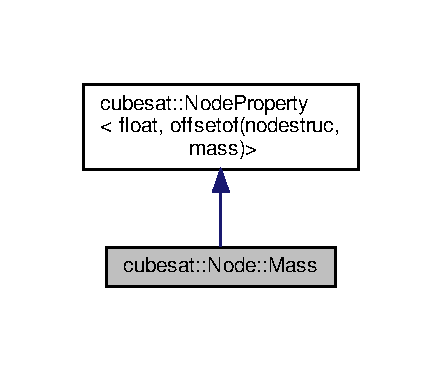
\includegraphics[width=212pt]{structcubesat_1_1Node_1_1Mass__inherit__graph}
\end{center}
\end{figure}


Collaboration diagram for cubesat\+:\+:Node\+:\+:Mass\+:
\nopagebreak
\begin{figure}[H]
\begin{center}
\leavevmode
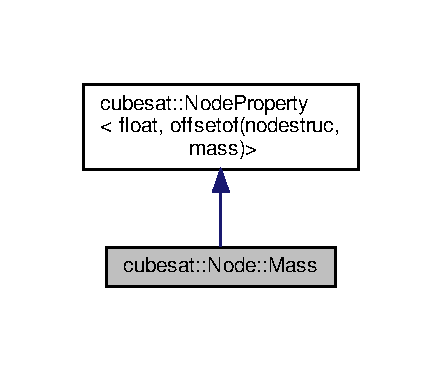
\includegraphics[width=212pt]{structcubesat_1_1Node_1_1Mass__coll__graph}
\end{center}
\end{figure}
\subsection*{Static Public Attributes}
\begin{DoxyCompactItemize}
\item 
static constexpr auto \hyperlink{structcubesat_1_1Node_1_1Mass_a4d87240a8d3d25bfeb5ec3e04bcdd6c4}{key} = \char`\"{}node\+\_\+mass\char`\"{}
\item 
static constexpr const char $\ast$ \hyperlink{structcubesat_1_1Node_1_1Mass_a032a7d325e46b57cd6ba184e1555d95b}{name} = \char`\"{}Mass\char`\"{}
\end{DoxyCompactItemize}
\subsection*{Additional Inherited Members}


\subsection{Member Data Documentation}
\mbox{\Hypertarget{structcubesat_1_1Node_1_1Mass_a4d87240a8d3d25bfeb5ec3e04bcdd6c4}\label{structcubesat_1_1Node_1_1Mass_a4d87240a8d3d25bfeb5ec3e04bcdd6c4}} 
\index{cubesat\+::\+Node\+::\+Mass@{cubesat\+::\+Node\+::\+Mass}!key@{key}}
\index{key@{key}!cubesat\+::\+Node\+::\+Mass@{cubesat\+::\+Node\+::\+Mass}}
\subsubsection{\texorpdfstring{key}{key}}
{\footnotesize\ttfamily constexpr auto cubesat\+::\+Node\+::\+Mass\+::key = \char`\"{}node\+\_\+mass\char`\"{}\hspace{0.3cm}{\ttfamily [static]}}

\mbox{\Hypertarget{structcubesat_1_1Node_1_1Mass_a032a7d325e46b57cd6ba184e1555d95b}\label{structcubesat_1_1Node_1_1Mass_a032a7d325e46b57cd6ba184e1555d95b}} 
\index{cubesat\+::\+Node\+::\+Mass@{cubesat\+::\+Node\+::\+Mass}!name@{name}}
\index{name@{name}!cubesat\+::\+Node\+::\+Mass@{cubesat\+::\+Node\+::\+Mass}}
\subsubsection{\texorpdfstring{name}{name}}
{\footnotesize\ttfamily constexpr const char$\ast$ cubesat\+::\+Node\+::\+Mass\+::name = \char`\"{}Mass\char`\"{}\hspace{0.3cm}{\ttfamily [static]}}



The documentation for this struct was generated from the following file\+:\begin{DoxyCompactItemize}
\item 
/home/osboxes/cosmos/source/projects/cubesat-\/kit/include/utility/\hyperlink{DeviceDetail_8h}{Device\+Detail.\+h}\end{DoxyCompactItemize}

\hypertarget{structcubesat_1_1PyCubed_1_1MessageHandler}{}\section{cubesat\+:\+:Py\+Cubed\+:\+:Message\+Handler Struct Reference}
\label{structcubesat_1_1PyCubed_1_1MessageHandler}\index{cubesat\+::\+Py\+Cubed\+::\+Message\+Handler@{cubesat\+::\+Py\+Cubed\+::\+Message\+Handler}}


Collaboration diagram for cubesat\+:\+:Py\+Cubed\+:\+:Message\+Handler\+:
\nopagebreak
\begin{figure}[H]
\begin{center}
\leavevmode
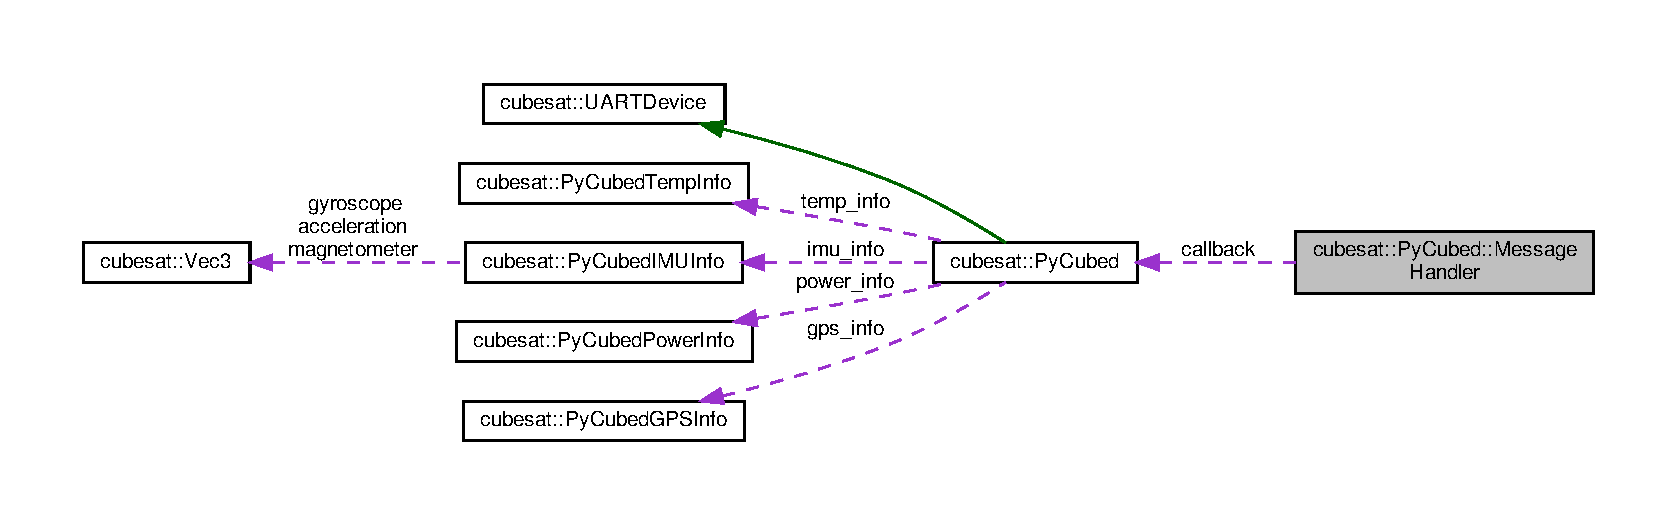
\includegraphics[width=350pt]{structcubesat_1_1PyCubed_1_1MessageHandler__coll__graph}
\end{center}
\end{figure}
\subsection*{Public Attributes}
\begin{DoxyCompactItemize}
\item 
\hyperlink{namespacecubesat_a3b98f17d41bf0e37fe0d382b897f9692}{Py\+Cubed\+Message\+Handler\+Callback} \hyperlink{structcubesat_1_1PyCubed_1_1MessageHandler_a9c4a599d7224add95ab56e915095497e}{callback}
\item 
unsigned int \hyperlink{structcubesat_1_1PyCubed_1_1MessageHandler_a42724ac13a929837460a2d1923f47514}{num\+\_\+args}
\end{DoxyCompactItemize}


\subsection{Member Data Documentation}
\mbox{\Hypertarget{structcubesat_1_1PyCubed_1_1MessageHandler_a9c4a599d7224add95ab56e915095497e}\label{structcubesat_1_1PyCubed_1_1MessageHandler_a9c4a599d7224add95ab56e915095497e}} 
\index{cubesat\+::\+Py\+Cubed\+::\+Message\+Handler@{cubesat\+::\+Py\+Cubed\+::\+Message\+Handler}!callback@{callback}}
\index{callback@{callback}!cubesat\+::\+Py\+Cubed\+::\+Message\+Handler@{cubesat\+::\+Py\+Cubed\+::\+Message\+Handler}}
\subsubsection{\texorpdfstring{callback}{callback}}
{\footnotesize\ttfamily \hyperlink{namespacecubesat_a3b98f17d41bf0e37fe0d382b897f9692}{Py\+Cubed\+Message\+Handler\+Callback} cubesat\+::\+Py\+Cubed\+::\+Message\+Handler\+::callback}

\mbox{\Hypertarget{structcubesat_1_1PyCubed_1_1MessageHandler_a42724ac13a929837460a2d1923f47514}\label{structcubesat_1_1PyCubed_1_1MessageHandler_a42724ac13a929837460a2d1923f47514}} 
\index{cubesat\+::\+Py\+Cubed\+::\+Message\+Handler@{cubesat\+::\+Py\+Cubed\+::\+Message\+Handler}!num\+\_\+args@{num\+\_\+args}}
\index{num\+\_\+args@{num\+\_\+args}!cubesat\+::\+Py\+Cubed\+::\+Message\+Handler@{cubesat\+::\+Py\+Cubed\+::\+Message\+Handler}}
\subsubsection{\texorpdfstring{num\+\_\+args}{num\_args}}
{\footnotesize\ttfamily unsigned int cubesat\+::\+Py\+Cubed\+::\+Message\+Handler\+::num\+\_\+args}



The documentation for this struct was generated from the following file\+:\begin{DoxyCompactItemize}
\item 
/home/osboxes/cosmos/source/projects/cubesat-\/kit/include/device/\hyperlink{PyCubed_8h}{Py\+Cubed.\+h}\end{DoxyCompactItemize}

\hypertarget{structcubesat_1_1PyCubed_1_1MessageParser}{}\section{cubesat\+:\+:Py\+Cubed\+:\+:Message\+Parser Struct Reference}
\label{structcubesat_1_1PyCubed_1_1MessageParser}\index{cubesat\+::\+Py\+Cubed\+::\+Message\+Parser@{cubesat\+::\+Py\+Cubed\+::\+Message\+Parser}}


Collaboration diagram for cubesat\+:\+:Py\+Cubed\+:\+:Message\+Parser\+:
\nopagebreak
\begin{figure}[H]
\begin{center}
\leavevmode
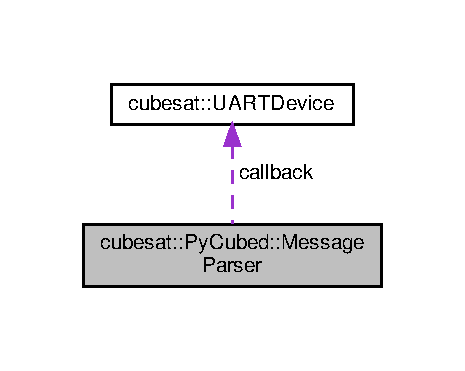
\includegraphics[width=223pt]{structcubesat_1_1PyCubed_1_1MessageParser__coll__graph}
\end{center}
\end{figure}
\subsection*{Public Attributes}
\begin{DoxyCompactItemize}
\item 
\hyperlink{namespacecubesat_ad7197c1bfb09998ced84827cb0dd1680}{Py\+Cubed\+Message\+Parser\+Callback} \hyperlink{structcubesat_1_1PyCubed_1_1MessageParser_aebe4576060c45c177677017e55f1a2db}{callback}
\end{DoxyCompactItemize}


\subsection{Member Data Documentation}
\mbox{\Hypertarget{structcubesat_1_1PyCubed_1_1MessageParser_aebe4576060c45c177677017e55f1a2db}\label{structcubesat_1_1PyCubed_1_1MessageParser_aebe4576060c45c177677017e55f1a2db}} 
\index{cubesat\+::\+Py\+Cubed\+::\+Message\+Parser@{cubesat\+::\+Py\+Cubed\+::\+Message\+Parser}!callback@{callback}}
\index{callback@{callback}!cubesat\+::\+Py\+Cubed\+::\+Message\+Parser@{cubesat\+::\+Py\+Cubed\+::\+Message\+Parser}}
\subsubsection{\texorpdfstring{callback}{callback}}
{\footnotesize\ttfamily \hyperlink{namespacecubesat_ad7197c1bfb09998ced84827cb0dd1680}{Py\+Cubed\+Message\+Parser\+Callback} cubesat\+::\+Py\+Cubed\+::\+Message\+Parser\+::callback}



The documentation for this struct was generated from the following file\+:\begin{DoxyCompactItemize}
\item 
/home/osboxes/cosmos/source/projects/cubesat-\/kit/include/device/\hyperlink{PyCubed_8h}{Py\+Cubed.\+h}\end{DoxyCompactItemize}

\hypertarget{structcubesat_1_1PyCubed_1_1MessageSender}{}\section{cubesat\+:\+:Py\+Cubed\+:\+:Message\+Sender Struct Reference}
\label{structcubesat_1_1PyCubed_1_1MessageSender}\index{cubesat\+::\+Py\+Cubed\+::\+Message\+Sender@{cubesat\+::\+Py\+Cubed\+::\+Message\+Sender}}
\subsection*{Public Attributes}
\begin{DoxyCompactItemize}
\item 
\hyperlink{namespacecubesat_a0cd8f3b1ff80acfd36cac73e8eb12b88}{Py\+Cubed\+Message\+Sender} \hyperlink{structcubesat_1_1PyCubed_1_1MessageSender_a42196732fdc5f0b25f988148ae419a57}{callback}
\end{DoxyCompactItemize}


\subsection{Member Data Documentation}
\mbox{\Hypertarget{structcubesat_1_1PyCubed_1_1MessageSender_a42196732fdc5f0b25f988148ae419a57}\label{structcubesat_1_1PyCubed_1_1MessageSender_a42196732fdc5f0b25f988148ae419a57}} 
\index{cubesat\+::\+Py\+Cubed\+::\+Message\+Sender@{cubesat\+::\+Py\+Cubed\+::\+Message\+Sender}!callback@{callback}}
\index{callback@{callback}!cubesat\+::\+Py\+Cubed\+::\+Message\+Sender@{cubesat\+::\+Py\+Cubed\+::\+Message\+Sender}}
\subsubsection{\texorpdfstring{callback}{callback}}
{\footnotesize\ttfamily \hyperlink{namespacecubesat_a0cd8f3b1ff80acfd36cac73e8eb12b88}{Py\+Cubed\+Message\+Sender} cubesat\+::\+Py\+Cubed\+::\+Message\+Sender\+::callback}



The documentation for this struct was generated from the following file\+:\begin{DoxyCompactItemize}
\item 
/home/osboxes/cosmos/source/projects/cubesat-\/kit/include/device/\hyperlink{PyCubed_8h}{Py\+Cubed.\+h}\end{DoxyCompactItemize}

\hypertarget{structcubesat_1_1Node_1_1MomentOfInertia}{}\section{cubesat\+:\+:Node\+:\+:Moment\+Of\+Inertia Struct Reference}
\label{structcubesat_1_1Node_1_1MomentOfInertia}\index{cubesat\+::\+Node\+::\+Moment\+Of\+Inertia@{cubesat\+::\+Node\+::\+Moment\+Of\+Inertia}}


{\ttfamily \#include $<$Device\+Detail.\+h$>$}



Inheritance diagram for cubesat\+:\+:Node\+:\+:Moment\+Of\+Inertia\+:
\nopagebreak
\begin{figure}[H]
\begin{center}
\leavevmode
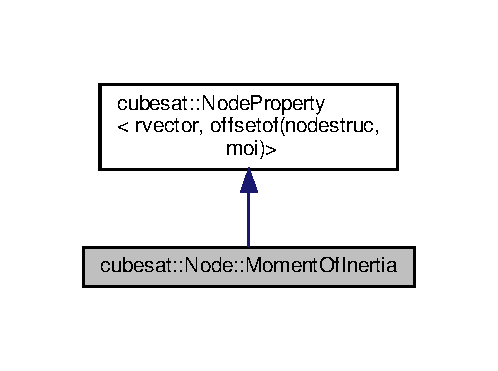
\includegraphics[width=239pt]{structcubesat_1_1Node_1_1MomentOfInertia__inherit__graph}
\end{center}
\end{figure}


Collaboration diagram for cubesat\+:\+:Node\+:\+:Moment\+Of\+Inertia\+:
\nopagebreak
\begin{figure}[H]
\begin{center}
\leavevmode
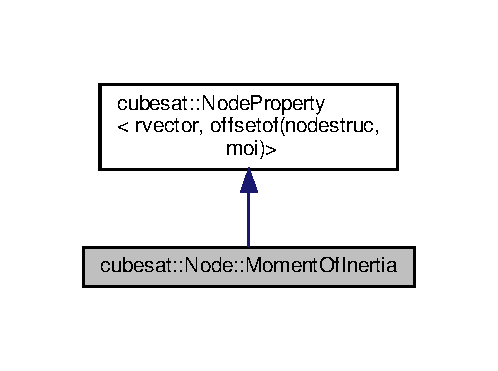
\includegraphics[width=239pt]{structcubesat_1_1Node_1_1MomentOfInertia__coll__graph}
\end{center}
\end{figure}
\subsection*{Static Public Attributes}
\begin{DoxyCompactItemize}
\item 
static constexpr auto \hyperlink{structcubesat_1_1Node_1_1MomentOfInertia_a728df4de3784819e48a002826e3b7d6e}{key} = \char`\"{}node\+\_\+moi\char`\"{}
\item 
static constexpr const char $\ast$ \hyperlink{structcubesat_1_1Node_1_1MomentOfInertia_aa2921ca8e0670caa8de1e09b47a82917}{name} = \char`\"{}Moment of Inertia\char`\"{}
\end{DoxyCompactItemize}
\subsection*{Additional Inherited Members}


\subsection{Member Data Documentation}
\mbox{\Hypertarget{structcubesat_1_1Node_1_1MomentOfInertia_a728df4de3784819e48a002826e3b7d6e}\label{structcubesat_1_1Node_1_1MomentOfInertia_a728df4de3784819e48a002826e3b7d6e}} 
\index{cubesat\+::\+Node\+::\+Moment\+Of\+Inertia@{cubesat\+::\+Node\+::\+Moment\+Of\+Inertia}!key@{key}}
\index{key@{key}!cubesat\+::\+Node\+::\+Moment\+Of\+Inertia@{cubesat\+::\+Node\+::\+Moment\+Of\+Inertia}}
\subsubsection{\texorpdfstring{key}{key}}
{\footnotesize\ttfamily constexpr auto cubesat\+::\+Node\+::\+Moment\+Of\+Inertia\+::key = \char`\"{}node\+\_\+moi\char`\"{}\hspace{0.3cm}{\ttfamily [static]}}

\mbox{\Hypertarget{structcubesat_1_1Node_1_1MomentOfInertia_aa2921ca8e0670caa8de1e09b47a82917}\label{structcubesat_1_1Node_1_1MomentOfInertia_aa2921ca8e0670caa8de1e09b47a82917}} 
\index{cubesat\+::\+Node\+::\+Moment\+Of\+Inertia@{cubesat\+::\+Node\+::\+Moment\+Of\+Inertia}!name@{name}}
\index{name@{name}!cubesat\+::\+Node\+::\+Moment\+Of\+Inertia@{cubesat\+::\+Node\+::\+Moment\+Of\+Inertia}}
\subsubsection{\texorpdfstring{name}{name}}
{\footnotesize\ttfamily constexpr const char$\ast$ cubesat\+::\+Node\+::\+Moment\+Of\+Inertia\+::name = \char`\"{}Moment of Inertia\char`\"{}\hspace{0.3cm}{\ttfamily [static]}}



The documentation for this struct was generated from the following file\+:\begin{DoxyCompactItemize}
\item 
/home/osboxes/cosmos/source/projects/cubesat-\/kit/include/utility/\hyperlink{DeviceDetail_8h}{Device\+Detail.\+h}\end{DoxyCompactItemize}

\hypertarget{classcubesat_1_1MultipleSimpleAgentException}{}\section{cubesat\+:\+:Multiple\+Simple\+Agent\+Exception Class Reference}
\label{classcubesat_1_1MultipleSimpleAgentException}\index{cubesat\+::\+Multiple\+Simple\+Agent\+Exception@{cubesat\+::\+Multiple\+Simple\+Agent\+Exception}}


Thrown if the user attempts to create a second \hyperlink{classcubesat_1_1SimpleAgent}{Simple\+Agent} in the same process.  




{\ttfamily \#include $<$Exceptions.\+h$>$}



Inheritance diagram for cubesat\+:\+:Multiple\+Simple\+Agent\+Exception\+:\nopagebreak
\begin{figure}[H]
\begin{center}
\leavevmode
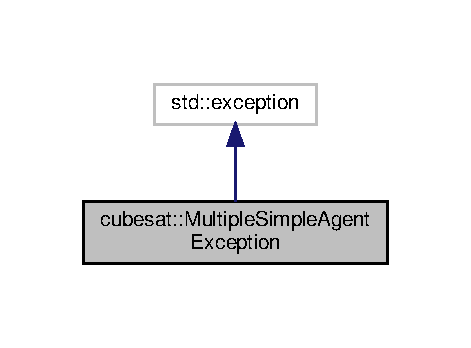
\includegraphics[width=226pt]{classcubesat_1_1MultipleSimpleAgentException__inherit__graph}
\end{center}
\end{figure}


Collaboration diagram for cubesat\+:\+:Multiple\+Simple\+Agent\+Exception\+:\nopagebreak
\begin{figure}[H]
\begin{center}
\leavevmode
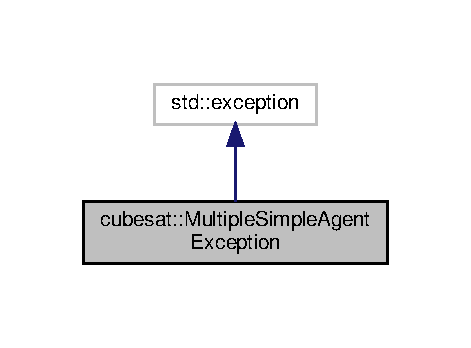
\includegraphics[width=226pt]{classcubesat_1_1MultipleSimpleAgentException__coll__graph}
\end{center}
\end{figure}
\subsection*{Public Member Functions}
\begin{DoxyCompactItemize}
\item 
\hyperlink{classcubesat_1_1MultipleSimpleAgentException_a5af0ba65456487dd0c08e5e0c764cccf}{Multiple\+Simple\+Agent\+Exception} (const std\+::string \&msg)
\item 
virtual const char $\ast$ \hyperlink{classcubesat_1_1MultipleSimpleAgentException_a01fc1d1216da063be9c5cf49e7885265}{what} () const  throw ()
\end{DoxyCompactItemize}
\subsection*{Private Attributes}
\begin{DoxyCompactItemize}
\item 
std\+::string \hyperlink{classcubesat_1_1MultipleSimpleAgentException_ab7a3c4ac9d8c35c62d5d91395c8d4576}{error\+\_\+msg}
\end{DoxyCompactItemize}


\subsection{Detailed Description}
Thrown if the user attempts to create a second \hyperlink{classcubesat_1_1SimpleAgent}{Simple\+Agent} in the same process. 

\subsection{Constructor \& Destructor Documentation}
\mbox{\Hypertarget{classcubesat_1_1MultipleSimpleAgentException_a5af0ba65456487dd0c08e5e0c764cccf}\label{classcubesat_1_1MultipleSimpleAgentException_a5af0ba65456487dd0c08e5e0c764cccf}} 
\index{cubesat\+::\+Multiple\+Simple\+Agent\+Exception@{cubesat\+::\+Multiple\+Simple\+Agent\+Exception}!Multiple\+Simple\+Agent\+Exception@{Multiple\+Simple\+Agent\+Exception}}
\index{Multiple\+Simple\+Agent\+Exception@{Multiple\+Simple\+Agent\+Exception}!cubesat\+::\+Multiple\+Simple\+Agent\+Exception@{cubesat\+::\+Multiple\+Simple\+Agent\+Exception}}
\subsubsection{\texorpdfstring{Multiple\+Simple\+Agent\+Exception()}{MultipleSimpleAgentException()}}
{\footnotesize\ttfamily cubesat\+::\+Multiple\+Simple\+Agent\+Exception\+::\+Multiple\+Simple\+Agent\+Exception (\begin{DoxyParamCaption}\item[{const std\+::string \&}]{msg }\end{DoxyParamCaption})\hspace{0.3cm}{\ttfamily [inline]}}



\subsection{Member Function Documentation}
\mbox{\Hypertarget{classcubesat_1_1MultipleSimpleAgentException_a01fc1d1216da063be9c5cf49e7885265}\label{classcubesat_1_1MultipleSimpleAgentException_a01fc1d1216da063be9c5cf49e7885265}} 
\index{cubesat\+::\+Multiple\+Simple\+Agent\+Exception@{cubesat\+::\+Multiple\+Simple\+Agent\+Exception}!what@{what}}
\index{what@{what}!cubesat\+::\+Multiple\+Simple\+Agent\+Exception@{cubesat\+::\+Multiple\+Simple\+Agent\+Exception}}
\subsubsection{\texorpdfstring{what()}{what()}}
{\footnotesize\ttfamily virtual const char$\ast$ cubesat\+::\+Multiple\+Simple\+Agent\+Exception\+::what (\begin{DoxyParamCaption}{ }\end{DoxyParamCaption}) const throw  ) \hspace{0.3cm}{\ttfamily [inline]}, {\ttfamily [virtual]}}



\subsection{Member Data Documentation}
\mbox{\Hypertarget{classcubesat_1_1MultipleSimpleAgentException_ab7a3c4ac9d8c35c62d5d91395c8d4576}\label{classcubesat_1_1MultipleSimpleAgentException_ab7a3c4ac9d8c35c62d5d91395c8d4576}} 
\index{cubesat\+::\+Multiple\+Simple\+Agent\+Exception@{cubesat\+::\+Multiple\+Simple\+Agent\+Exception}!error\+\_\+msg@{error\+\_\+msg}}
\index{error\+\_\+msg@{error\+\_\+msg}!cubesat\+::\+Multiple\+Simple\+Agent\+Exception@{cubesat\+::\+Multiple\+Simple\+Agent\+Exception}}
\subsubsection{\texorpdfstring{error\+\_\+msg}{error\_msg}}
{\footnotesize\ttfamily std\+::string cubesat\+::\+Multiple\+Simple\+Agent\+Exception\+::error\+\_\+msg\hspace{0.3cm}{\ttfamily [private]}}



The documentation for this class was generated from the following file\+:\begin{DoxyCompactItemize}
\item 
/home/osboxes/cosmos/source/projects/cubesat-\/kit/include/utility/\hyperlink{Exceptions_8h}{Exceptions.\+h}\end{DoxyCompactItemize}

\hypertarget{structcubesat_1_1SimpleAgent_1_1NodeProperty}{}\section{cubesat\+:\+:Simple\+Agent\+:\+:Node\+Property Struct Reference}
\label{structcubesat_1_1SimpleAgent_1_1NodeProperty}\index{cubesat\+::\+Simple\+Agent\+::\+Node\+Property@{cubesat\+::\+Simple\+Agent\+::\+Node\+Property}}


Represents a C\+O\+S\+M\+OS node property.  




{\ttfamily \#include $<$Simple\+Agent.\+h$>$}

\subsection*{Public Member Functions}
\begin{DoxyCompactItemize}
\item 
\hyperlink{structcubesat_1_1SimpleAgent_1_1NodeProperty_a381db507c0ff0f09dd6ad5f4b93743a8}{Node\+Property} ()
\begin{DoxyCompactList}\small\item\em A default constructor is required for std\+::unordered\+\_\+map. \end{DoxyCompactList}\item 
\hyperlink{structcubesat_1_1SimpleAgent_1_1NodeProperty_aa79f92a0bebd44ca9339780dd682d69d}{Node\+Property} (const std\+::string \&\hyperlink{structcubesat_1_1SimpleAgent_1_1NodeProperty_aede92ae1ce895354a2cd9995cd7a8d6f}{value\+\_\+string}, const std\+::string \&\hyperlink{structcubesat_1_1SimpleAgent_1_1NodeProperty_a6d3e8b9ad7ceba4dadbb90c036c3bd15}{cosmos\+\_\+name}, const std\+::string \&\hyperlink{structcubesat_1_1SimpleAgent_1_1NodeProperty_a7251c568d143b84af02872dcc812b29c}{readable\+\_\+name}, bool \hyperlink{structcubesat_1_1SimpleAgent_1_1NodeProperty_a4e346ca338dcf56d731b5455895afa39}{post})
\end{DoxyCompactItemize}
\subsection*{Public Attributes}
\begin{DoxyCompactItemize}
\item 
std\+::string \hyperlink{structcubesat_1_1SimpleAgent_1_1NodeProperty_a6d3e8b9ad7ceba4dadbb90c036c3bd15}{cosmos\+\_\+name}
\begin{DoxyCompactList}\small\item\em The C\+O\+S\+M\+OS name of the property (e.\+g. node\+\_\+battcap) \end{DoxyCompactList}\item 
std\+::string \hyperlink{structcubesat_1_1SimpleAgent_1_1NodeProperty_a7251c568d143b84af02872dcc812b29c}{readable\+\_\+name}
\begin{DoxyCompactList}\small\item\em The readable name of the property (e.\+g. \hyperlink{classcubesat_1_1Battery}{Battery} Capacity) \end{DoxyCompactList}\item 
std\+::string \hyperlink{structcubesat_1_1SimpleAgent_1_1NodeProperty_aede92ae1ce895354a2cd9995cd7a8d6f}{value\+\_\+string}
\begin{DoxyCompactList}\small\item\em The value of the property represented as a string. \end{DoxyCompactList}\item 
bool \hyperlink{structcubesat_1_1SimpleAgent_1_1NodeProperty_a4e346ca338dcf56d731b5455895afa39}{post}
\begin{DoxyCompactList}\small\item\em Whether or not the property should be posted in the state of health string. \end{DoxyCompactList}\end{DoxyCompactItemize}


\subsection{Detailed Description}
Represents a C\+O\+S\+M\+OS node property. 

\subsection{Constructor \& Destructor Documentation}
\mbox{\Hypertarget{structcubesat_1_1SimpleAgent_1_1NodeProperty_a381db507c0ff0f09dd6ad5f4b93743a8}\label{structcubesat_1_1SimpleAgent_1_1NodeProperty_a381db507c0ff0f09dd6ad5f4b93743a8}} 
\index{cubesat\+::\+Simple\+Agent\+::\+Node\+Property@{cubesat\+::\+Simple\+Agent\+::\+Node\+Property}!Node\+Property@{Node\+Property}}
\index{Node\+Property@{Node\+Property}!cubesat\+::\+Simple\+Agent\+::\+Node\+Property@{cubesat\+::\+Simple\+Agent\+::\+Node\+Property}}
\subsubsection{\texorpdfstring{Node\+Property()}{NodeProperty()}\hspace{0.1cm}{\footnotesize\ttfamily [1/2]}}
{\footnotesize\ttfamily cubesat\+::\+Simple\+Agent\+::\+Node\+Property\+::\+Node\+Property (\begin{DoxyParamCaption}{ }\end{DoxyParamCaption})\hspace{0.3cm}{\ttfamily [inline]}}



A default constructor is required for std\+::unordered\+\_\+map. 

\mbox{\Hypertarget{structcubesat_1_1SimpleAgent_1_1NodeProperty_aa79f92a0bebd44ca9339780dd682d69d}\label{structcubesat_1_1SimpleAgent_1_1NodeProperty_aa79f92a0bebd44ca9339780dd682d69d}} 
\index{cubesat\+::\+Simple\+Agent\+::\+Node\+Property@{cubesat\+::\+Simple\+Agent\+::\+Node\+Property}!Node\+Property@{Node\+Property}}
\index{Node\+Property@{Node\+Property}!cubesat\+::\+Simple\+Agent\+::\+Node\+Property@{cubesat\+::\+Simple\+Agent\+::\+Node\+Property}}
\subsubsection{\texorpdfstring{Node\+Property()}{NodeProperty()}\hspace{0.1cm}{\footnotesize\ttfamily [2/2]}}
{\footnotesize\ttfamily cubesat\+::\+Simple\+Agent\+::\+Node\+Property\+::\+Node\+Property (\begin{DoxyParamCaption}\item[{const std\+::string \&}]{value\+\_\+string,  }\item[{const std\+::string \&}]{cosmos\+\_\+name,  }\item[{const std\+::string \&}]{readable\+\_\+name,  }\item[{bool}]{post }\end{DoxyParamCaption})\hspace{0.3cm}{\ttfamily [inline]}}



\subsection{Member Data Documentation}
\mbox{\Hypertarget{structcubesat_1_1SimpleAgent_1_1NodeProperty_a6d3e8b9ad7ceba4dadbb90c036c3bd15}\label{structcubesat_1_1SimpleAgent_1_1NodeProperty_a6d3e8b9ad7ceba4dadbb90c036c3bd15}} 
\index{cubesat\+::\+Simple\+Agent\+::\+Node\+Property@{cubesat\+::\+Simple\+Agent\+::\+Node\+Property}!cosmos\+\_\+name@{cosmos\+\_\+name}}
\index{cosmos\+\_\+name@{cosmos\+\_\+name}!cubesat\+::\+Simple\+Agent\+::\+Node\+Property@{cubesat\+::\+Simple\+Agent\+::\+Node\+Property}}
\subsubsection{\texorpdfstring{cosmos\+\_\+name}{cosmos\_name}}
{\footnotesize\ttfamily std\+::string cubesat\+::\+Simple\+Agent\+::\+Node\+Property\+::cosmos\+\_\+name}



The C\+O\+S\+M\+OS name of the property (e.\+g. node\+\_\+battcap) 

\mbox{\Hypertarget{structcubesat_1_1SimpleAgent_1_1NodeProperty_a4e346ca338dcf56d731b5455895afa39}\label{structcubesat_1_1SimpleAgent_1_1NodeProperty_a4e346ca338dcf56d731b5455895afa39}} 
\index{cubesat\+::\+Simple\+Agent\+::\+Node\+Property@{cubesat\+::\+Simple\+Agent\+::\+Node\+Property}!post@{post}}
\index{post@{post}!cubesat\+::\+Simple\+Agent\+::\+Node\+Property@{cubesat\+::\+Simple\+Agent\+::\+Node\+Property}}
\subsubsection{\texorpdfstring{post}{post}}
{\footnotesize\ttfamily bool cubesat\+::\+Simple\+Agent\+::\+Node\+Property\+::post}



Whether or not the property should be posted in the state of health string. 

\mbox{\Hypertarget{structcubesat_1_1SimpleAgent_1_1NodeProperty_a7251c568d143b84af02872dcc812b29c}\label{structcubesat_1_1SimpleAgent_1_1NodeProperty_a7251c568d143b84af02872dcc812b29c}} 
\index{cubesat\+::\+Simple\+Agent\+::\+Node\+Property@{cubesat\+::\+Simple\+Agent\+::\+Node\+Property}!readable\+\_\+name@{readable\+\_\+name}}
\index{readable\+\_\+name@{readable\+\_\+name}!cubesat\+::\+Simple\+Agent\+::\+Node\+Property@{cubesat\+::\+Simple\+Agent\+::\+Node\+Property}}
\subsubsection{\texorpdfstring{readable\+\_\+name}{readable\_name}}
{\footnotesize\ttfamily std\+::string cubesat\+::\+Simple\+Agent\+::\+Node\+Property\+::readable\+\_\+name}



The readable name of the property (e.\+g. \hyperlink{classcubesat_1_1Battery}{Battery} Capacity) 

\mbox{\Hypertarget{structcubesat_1_1SimpleAgent_1_1NodeProperty_aede92ae1ce895354a2cd9995cd7a8d6f}\label{structcubesat_1_1SimpleAgent_1_1NodeProperty_aede92ae1ce895354a2cd9995cd7a8d6f}} 
\index{cubesat\+::\+Simple\+Agent\+::\+Node\+Property@{cubesat\+::\+Simple\+Agent\+::\+Node\+Property}!value\+\_\+string@{value\+\_\+string}}
\index{value\+\_\+string@{value\+\_\+string}!cubesat\+::\+Simple\+Agent\+::\+Node\+Property@{cubesat\+::\+Simple\+Agent\+::\+Node\+Property}}
\subsubsection{\texorpdfstring{value\+\_\+string}{value\_string}}
{\footnotesize\ttfamily std\+::string cubesat\+::\+Simple\+Agent\+::\+Node\+Property\+::value\+\_\+string}



The value of the property represented as a string. 



The documentation for this struct was generated from the following file\+:\begin{DoxyCompactItemize}
\item 
/home/osboxes/cosmos/source/projects/cubesat-\/kit/include/utility/\hyperlink{SimpleAgent_8h}{Simple\+Agent.\+h}\end{DoxyCompactItemize}

\hypertarget{structcubesat_1_1NodeProperty}{}\section{cubesat\+:\+:Node\+Property$<$ T, \+\_\+offset $>$ Struct Template Reference}
\label{structcubesat_1_1NodeProperty}\index{cubesat\+::\+Node\+Property$<$ T, \+\_\+offset $>$@{cubesat\+::\+Node\+Property$<$ T, \+\_\+offset $>$}}


{\ttfamily \#include $<$Device\+Detail.\+h$>$}

\subsection*{Public Types}
\begin{DoxyCompactItemize}
\item 
using \hyperlink{structcubesat_1_1NodeProperty_a8d6d9fdbd56b8fdc2fe2c3b80f54846a}{Value\+Type} = T
\begin{DoxyCompactList}\small\item\em The value type. \end{DoxyCompactList}\end{DoxyCompactItemize}
\subsection*{Static Public Attributes}
\begin{DoxyCompactItemize}
\item 
static constexpr size\+\_\+t \hyperlink{structcubesat_1_1NodeProperty_a028759af3a77611ebdcbd3e4f352bfa0}{offset} = \+\_\+offset
\begin{DoxyCompactList}\small\item\em The byte offset to the property member. \end{DoxyCompactList}\end{DoxyCompactItemize}


\subsection{Member Typedef Documentation}
\mbox{\Hypertarget{structcubesat_1_1NodeProperty_a8d6d9fdbd56b8fdc2fe2c3b80f54846a}\label{structcubesat_1_1NodeProperty_a8d6d9fdbd56b8fdc2fe2c3b80f54846a}} 
\index{cubesat\+::\+Node\+Property@{cubesat\+::\+Node\+Property}!Value\+Type@{Value\+Type}}
\index{Value\+Type@{Value\+Type}!cubesat\+::\+Node\+Property@{cubesat\+::\+Node\+Property}}
\subsubsection{\texorpdfstring{Value\+Type}{ValueType}}
{\footnotesize\ttfamily template$<$typename T, size\+\_\+t \+\_\+offset$>$ \\
using \hyperlink{structcubesat_1_1NodeProperty}{cubesat\+::\+Node\+Property}$<$ T, \+\_\+offset $>$\+::\hyperlink{structcubesat_1_1NodeProperty_a8d6d9fdbd56b8fdc2fe2c3b80f54846a}{Value\+Type} =  T}



The value type. 



\subsection{Member Data Documentation}
\mbox{\Hypertarget{structcubesat_1_1NodeProperty_a028759af3a77611ebdcbd3e4f352bfa0}\label{structcubesat_1_1NodeProperty_a028759af3a77611ebdcbd3e4f352bfa0}} 
\index{cubesat\+::\+Node\+Property@{cubesat\+::\+Node\+Property}!offset@{offset}}
\index{offset@{offset}!cubesat\+::\+Node\+Property@{cubesat\+::\+Node\+Property}}
\subsubsection{\texorpdfstring{offset}{offset}}
{\footnotesize\ttfamily template$<$typename T, size\+\_\+t \+\_\+offset$>$ \\
constexpr size\+\_\+t \hyperlink{structcubesat_1_1NodeProperty}{cubesat\+::\+Node\+Property}$<$ T, \+\_\+offset $>$\+::offset = \+\_\+offset\hspace{0.3cm}{\ttfamily [static]}}



The byte offset to the property member. 



The documentation for this struct was generated from the following file\+:\begin{DoxyCompactItemize}
\item 
/home/osboxes/cosmos/source/projects/cubesat-\/kit/include/utility/\hyperlink{DeviceDetail_8h}{Device\+Detail.\+h}\end{DoxyCompactItemize}

\hypertarget{structcubesat_1_1SimpleAgent_1_1NonArgumentedRequestData}{}\section{cubesat\+:\+:Simple\+Agent\+:\+:Non\+Argumented\+Request\+Data Struct Reference}
\label{structcubesat_1_1SimpleAgent_1_1NonArgumentedRequestData}\index{cubesat\+::\+Simple\+Agent\+::\+Non\+Argumented\+Request\+Data@{cubesat\+::\+Simple\+Agent\+::\+Non\+Argumented\+Request\+Data}}


Stores data for a request with no arguments.  




{\ttfamily \#include $<$Simple\+Agent.\+h$>$}

\subsection*{Public Attributes}
\begin{DoxyCompactItemize}
\item 
\hyperlink{namespacecubesat_a494b2feec3d999510e5772da5c0b354c}{Non\+Argumented\+Request} \hyperlink{structcubesat_1_1SimpleAgent_1_1NonArgumentedRequestData_abda7d359fbd1212e306fe42b6bb5923f}{callback}
\end{DoxyCompactItemize}


\subsection{Detailed Description}
Stores data for a request with no arguments. 

\subsection{Member Data Documentation}
\mbox{\Hypertarget{structcubesat_1_1SimpleAgent_1_1NonArgumentedRequestData_abda7d359fbd1212e306fe42b6bb5923f}\label{structcubesat_1_1SimpleAgent_1_1NonArgumentedRequestData_abda7d359fbd1212e306fe42b6bb5923f}} 
\index{cubesat\+::\+Simple\+Agent\+::\+Non\+Argumented\+Request\+Data@{cubesat\+::\+Simple\+Agent\+::\+Non\+Argumented\+Request\+Data}!callback@{callback}}
\index{callback@{callback}!cubesat\+::\+Simple\+Agent\+::\+Non\+Argumented\+Request\+Data@{cubesat\+::\+Simple\+Agent\+::\+Non\+Argumented\+Request\+Data}}
\subsubsection{\texorpdfstring{callback}{callback}}
{\footnotesize\ttfamily \hyperlink{namespacecubesat_a494b2feec3d999510e5772da5c0b354c}{Non\+Argumented\+Request} cubesat\+::\+Simple\+Agent\+::\+Non\+Argumented\+Request\+Data\+::callback}



The documentation for this struct was generated from the following file\+:\begin{DoxyCompactItemize}
\item 
/home/osboxes/cosmos/source/projects/cubesat-\/kit/include/utility/\hyperlink{SimpleAgent_8h}{Simple\+Agent.\+h}\end{DoxyCompactItemize}

\hypertarget{classcubesat_1_1NonExistentPropertyException}{}\section{cubesat\+:\+:Non\+Existent\+Property\+Exception Class Reference}
\label{classcubesat_1_1NonExistentPropertyException}\index{cubesat\+::\+Non\+Existent\+Property\+Exception@{cubesat\+::\+Non\+Existent\+Property\+Exception}}


Thrown if a non-\/existent property is accessed.  




{\ttfamily \#include $<$Exceptions.\+h$>$}



Inheritance diagram for cubesat\+:\+:Non\+Existent\+Property\+Exception\+:\nopagebreak
\begin{figure}[H]
\begin{center}
\leavevmode
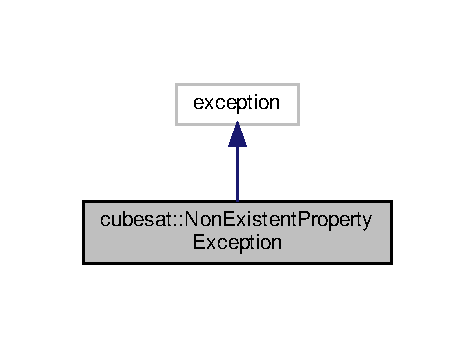
\includegraphics[width=228pt]{classcubesat_1_1NonExistentPropertyException__inherit__graph}
\end{center}
\end{figure}


Collaboration diagram for cubesat\+:\+:Non\+Existent\+Property\+Exception\+:\nopagebreak
\begin{figure}[H]
\begin{center}
\leavevmode
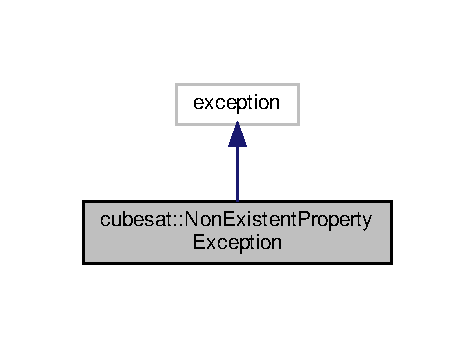
\includegraphics[width=228pt]{classcubesat_1_1NonExistentPropertyException__coll__graph}
\end{center}
\end{figure}
\subsection*{Public Member Functions}
\begin{DoxyCompactItemize}
\item 
\hyperlink{classcubesat_1_1NonExistentPropertyException_ac2d60c530b7838ec136e68193caad115}{Non\+Existent\+Property\+Exception} (const std\+::string \&prop\+\_\+name)
\item 
virtual const char $\ast$ \hyperlink{classcubesat_1_1NonExistentPropertyException_a160909d63d9d602a4151e32d8719ec58}{what} () const  throw ()
\end{DoxyCompactItemize}
\subsection*{Private Attributes}
\begin{DoxyCompactItemize}
\item 
std\+::string \hyperlink{classcubesat_1_1NonExistentPropertyException_a31c5141863cf737c22e0c1f5a8b05375}{error\+\_\+msg}
\end{DoxyCompactItemize}


\subsection{Detailed Description}
Thrown if a non-\/existent property is accessed. 

\subsection{Constructor \& Destructor Documentation}
\mbox{\Hypertarget{classcubesat_1_1NonExistentPropertyException_ac2d60c530b7838ec136e68193caad115}\label{classcubesat_1_1NonExistentPropertyException_ac2d60c530b7838ec136e68193caad115}} 
\index{cubesat\+::\+Non\+Existent\+Property\+Exception@{cubesat\+::\+Non\+Existent\+Property\+Exception}!Non\+Existent\+Property\+Exception@{Non\+Existent\+Property\+Exception}}
\index{Non\+Existent\+Property\+Exception@{Non\+Existent\+Property\+Exception}!cubesat\+::\+Non\+Existent\+Property\+Exception@{cubesat\+::\+Non\+Existent\+Property\+Exception}}
\subsubsection{\texorpdfstring{Non\+Existent\+Property\+Exception()}{NonExistentPropertyException()}}
{\footnotesize\ttfamily cubesat\+::\+Non\+Existent\+Property\+Exception\+::\+Non\+Existent\+Property\+Exception (\begin{DoxyParamCaption}\item[{const std\+::string \&}]{prop\+\_\+name }\end{DoxyParamCaption})\hspace{0.3cm}{\ttfamily [inline]}}



\subsection{Member Function Documentation}
\mbox{\Hypertarget{classcubesat_1_1NonExistentPropertyException_a160909d63d9d602a4151e32d8719ec58}\label{classcubesat_1_1NonExistentPropertyException_a160909d63d9d602a4151e32d8719ec58}} 
\index{cubesat\+::\+Non\+Existent\+Property\+Exception@{cubesat\+::\+Non\+Existent\+Property\+Exception}!what@{what}}
\index{what@{what}!cubesat\+::\+Non\+Existent\+Property\+Exception@{cubesat\+::\+Non\+Existent\+Property\+Exception}}
\subsubsection{\texorpdfstring{what()}{what()}}
{\footnotesize\ttfamily virtual const char$\ast$ cubesat\+::\+Non\+Existent\+Property\+Exception\+::what (\begin{DoxyParamCaption}{ }\end{DoxyParamCaption}) const throw  ) \hspace{0.3cm}{\ttfamily [inline]}, {\ttfamily [virtual]}}



\subsection{Member Data Documentation}
\mbox{\Hypertarget{classcubesat_1_1NonExistentPropertyException_a31c5141863cf737c22e0c1f5a8b05375}\label{classcubesat_1_1NonExistentPropertyException_a31c5141863cf737c22e0c1f5a8b05375}} 
\index{cubesat\+::\+Non\+Existent\+Property\+Exception@{cubesat\+::\+Non\+Existent\+Property\+Exception}!error\+\_\+msg@{error\+\_\+msg}}
\index{error\+\_\+msg@{error\+\_\+msg}!cubesat\+::\+Non\+Existent\+Property\+Exception@{cubesat\+::\+Non\+Existent\+Property\+Exception}}
\subsubsection{\texorpdfstring{error\+\_\+msg}{error\_msg}}
{\footnotesize\ttfamily std\+::string cubesat\+::\+Non\+Existent\+Property\+Exception\+::error\+\_\+msg\hspace{0.3cm}{\ttfamily [private]}}



The documentation for this class was generated from the following file\+:\begin{DoxyCompactItemize}
\item 
/home/osboxes/cosmos/source/projects/cubesat-\/kit/include/utility/\hyperlink{Exceptions_8h}{Exceptions.\+h}\end{DoxyCompactItemize}

\hypertarget{classcubesat_1_1OPT3001}{}\section{cubesat\+:\+:O\+P\+T3001 Class Reference}
\label{classcubesat_1_1OPT3001}\index{cubesat\+::\+O\+P\+T3001@{cubesat\+::\+O\+P\+T3001}}


Provides access to the \hyperlink{classcubesat_1_1OPT3001}{O\+P\+T3001} temperature sensor.  




{\ttfamily \#include $<$O\+P\+T3001.\+h$>$}



Inheritance diagram for cubesat\+:\+:O\+P\+T3001\+:\nopagebreak
\begin{figure}[H]
\begin{center}
\leavevmode
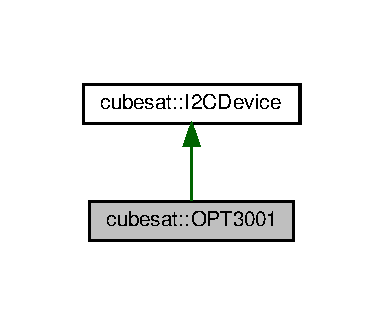
\includegraphics[width=184pt]{classcubesat_1_1OPT3001__inherit__graph}
\end{center}
\end{figure}


Collaboration diagram for cubesat\+:\+:O\+P\+T3001\+:\nopagebreak
\begin{figure}[H]
\begin{center}
\leavevmode
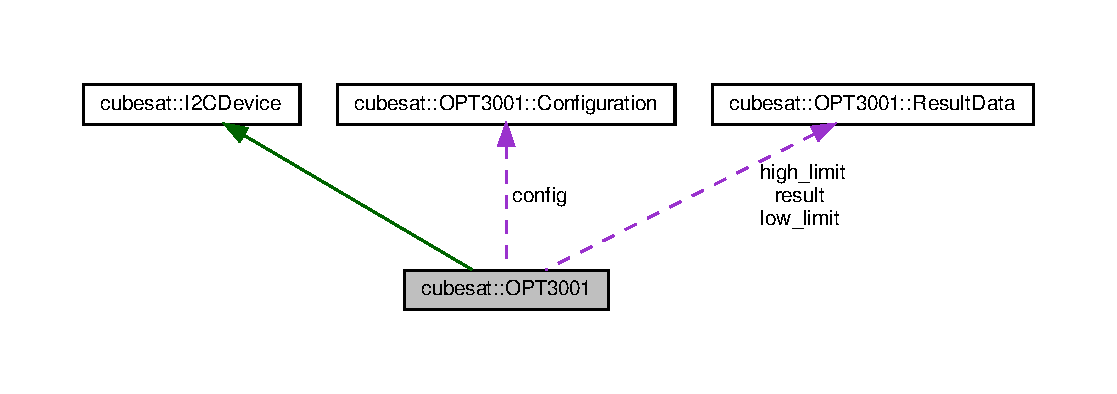
\includegraphics[width=350pt]{classcubesat_1_1OPT3001__coll__graph}
\end{center}
\end{figure}
\subsection*{Classes}
\begin{DoxyCompactItemize}
\item 
union \hyperlink{unioncubesat_1_1OPT3001_1_1Configuration}{Configuration}
\begin{DoxyCompactList}\small\item\em \hyperlink{unioncubesat_1_1OPT3001_1_1Configuration}{Configuration} flags corresponding to the configuration register on the device. \end{DoxyCompactList}\item 
union \hyperlink{unioncubesat_1_1OPT3001_1_1DeviceID}{Device\+ID}
\begin{DoxyCompactList}\small\item\em Stores data pulled from the result register. \end{DoxyCompactList}\item 
union \hyperlink{unioncubesat_1_1OPT3001_1_1ResultData}{Result\+Data}
\begin{DoxyCompactList}\small\item\em Stores data pulled from the result register. \end{DoxyCompactList}\end{DoxyCompactItemize}
\subsection*{Public Types}
\begin{DoxyCompactItemize}
\item 
enum \hyperlink{classcubesat_1_1OPT3001_af8ded2d0275e87105725928dc0485ad7}{Register} \+: uint8\+\_\+t \{ \newline
\hyperlink{classcubesat_1_1OPT3001_af8ded2d0275e87105725928dc0485ad7a8eea62084ca7e541d918e823422bd82e}{Register\+::\+Result} = 0x00, 
\hyperlink{classcubesat_1_1OPT3001_af8ded2d0275e87105725928dc0485ad7afa535ffb25e1fd20341652f9be21e06e}{Register\+::\+Config} = 0x01, 
\hyperlink{classcubesat_1_1OPT3001_af8ded2d0275e87105725928dc0485ad7adc3cf632a3bd74f489cf2c107ed4828b}{Register\+::\+Low\+Limit} = 0x02, 
\hyperlink{classcubesat_1_1OPT3001_af8ded2d0275e87105725928dc0485ad7aad4a6d393859661965ecfede46dcc2af}{Register\+::\+High\+Limit} = 0x03, 
\newline
\hyperlink{classcubesat_1_1OPT3001_af8ded2d0275e87105725928dc0485ad7ac0bd7654d5b278e65f21cf4e9153fdb4}{Register\+::\+Manufacturer} = 0x7E, 
\hyperlink{classcubesat_1_1OPT3001_af8ded2d0275e87105725928dc0485ad7ae1227e600b90b8a261c760fbaaaa5c97}{Register\+::\+Device\+ID} = 0x7F
 \}\begin{DoxyCompactList}\small\item\em Register addresses. \end{DoxyCompactList}
\end{DoxyCompactItemize}
\subsection*{Public Member Functions}
\begin{DoxyCompactItemize}
\item 
\hyperlink{classcubesat_1_1OPT3001_af8e948ecc4d4979484f226c48dcf4285}{O\+P\+T3001} ()
\item 
\hyperlink{classcubesat_1_1OPT3001_a0c985e7f3634b077e4b3955cb3c41b95}{O\+P\+T3001} (uint8\+\_\+t \hyperlink{classcubesat_1_1I2CDevice_acc13c6328bb7f29ddc5b9436d6b40816}{bus}, uint8\+\_\+t \hyperlink{classcubesat_1_1I2CDevice_a59cdefbd8b9720d194254c617f5c9b07}{device})
\begin{DoxyCompactList}\small\item\em Constructs a new \hyperlink{classcubesat_1_1OPT3001}{O\+P\+T3001} with the given bus and device numbers. \end{DoxyCompactList}\item 
\hyperlink{classcubesat_1_1OPT3001_ad2a4f35373ae73e42635ec261dc86e56}{O\+P\+T3001} (const \hyperlink{classcubesat_1_1OPT3001}{O\+P\+T3001} \&other)=delete
\item 
virtual \hyperlink{classcubesat_1_1OPT3001_af852a60be53aa8585ff8d1346ec5fa76}{$\sim$\+O\+P\+T3001} ()
\begin{DoxyCompactList}\small\item\em Destructor. \end{DoxyCompactList}\item 
void \hyperlink{classcubesat_1_1OPT3001_afb44b36406326e3af20a4cf63602baa7}{Read\+State} ()
\begin{DoxyCompactList}\small\item\em Updates information by reading device registers. \end{DoxyCompactList}\item 
bool \hyperlink{classcubesat_1_1OPT3001_a6df0cf4e46e38bbe9909f8e905b7540e}{Set\+Configuration} (\hyperlink{unioncubesat_1_1OPT3001_1_1Configuration}{Configuration} \hyperlink{classcubesat_1_1OPT3001_acf76526638ac9210adb947fa6b4b155f}{config})
\begin{DoxyCompactList}\small\item\em Writes the configuration data. \end{DoxyCompactList}\item 
\hyperlink{unioncubesat_1_1OPT3001_1_1Configuration}{Configuration} \hyperlink{classcubesat_1_1OPT3001_a19a22f506667bae934b78e588db9db70}{Get\+Configuration} () const
\begin{DoxyCompactList}\small\item\em Returns configuration details for this device. \end{DoxyCompactList}\item 
float \hyperlink{classcubesat_1_1OPT3001_a087a57d80f6e3f8d1ba8a0972e30e588}{Get\+Lux} () const
\begin{DoxyCompactList}\small\item\em Retrieves the latest lux reading. \end{DoxyCompactList}\item 
float \hyperlink{classcubesat_1_1OPT3001_a014e0389a3877b2fb4536c925579afd0}{Get\+High\+Limit} () const
\begin{DoxyCompactList}\small\item\em Retrieves the upper limit for lux. \end{DoxyCompactList}\item 
float \hyperlink{classcubesat_1_1OPT3001_acb7a4c2d524e89542598e09d4ba9237d}{Get\+Low\+Limit} () const
\begin{DoxyCompactList}\small\item\em Retrieves the lower limit for lux. \end{DoxyCompactList}\item 
\hyperlink{unioncubesat_1_1OPT3001_1_1ResultData}{Result\+Data} \hyperlink{classcubesat_1_1OPT3001_a0ae711185114bda442826f2afb8e5abe}{Get\+Result\+Register} () const
\item 
\hyperlink{unioncubesat_1_1OPT3001_1_1ResultData}{Result\+Data} \hyperlink{classcubesat_1_1OPT3001_a179490e36d96c976a174cc27ff9c56fe}{Get\+Low\+Limit\+Register} () const
\item 
\hyperlink{unioncubesat_1_1OPT3001_1_1ResultData}{Result\+Data} \hyperlink{classcubesat_1_1OPT3001_a2d6066e4ab634e0c1fa8094ec220be44}{Get\+High\+Limit\+Register} () const
\item 
uint16\+\_\+t \hyperlink{classcubesat_1_1OPT3001_a7d97464978c89d00212fa391e7c700d9}{Get\+Manufacturer\+ID} () const
\item 
uint16\+\_\+t \hyperlink{classcubesat_1_1OPT3001_adc2eb69ceb5e0f3448b06f199d2ec985}{Get\+Device\+ID} () const
\end{DoxyCompactItemize}
\subsection*{Private Attributes}
\begin{DoxyCompactItemize}
\item 
\hyperlink{unioncubesat_1_1OPT3001_1_1ResultData}{Result\+Data} \hyperlink{classcubesat_1_1OPT3001_a7eee3af72ef6914189ba433416388a8f}{result}
\item 
\hyperlink{unioncubesat_1_1OPT3001_1_1ResultData}{Result\+Data} \hyperlink{classcubesat_1_1OPT3001_a199e1dbf3a86211403e3f9bd286c27c5}{low\+\_\+limit}
\item 
\hyperlink{unioncubesat_1_1OPT3001_1_1ResultData}{Result\+Data} \hyperlink{classcubesat_1_1OPT3001_a8845a818c246527edaa414ddf59ff9a6}{high\+\_\+limit}
\item 
\hyperlink{unioncubesat_1_1OPT3001_1_1Configuration}{Configuration} \hyperlink{classcubesat_1_1OPT3001_acf76526638ac9210adb947fa6b4b155f}{config}
\item 
uint16\+\_\+t \hyperlink{classcubesat_1_1OPT3001_a5b5aa666cb00efe6f26d440965d055a7}{manufacturer\+\_\+id}
\item 
uint16\+\_\+t \hyperlink{classcubesat_1_1OPT3001_ab7240590fe1e63a4b4884ccdd603c243}{device\+\_\+id}
\end{DoxyCompactItemize}
\subsection*{Additional Inherited Members}


\subsection{Detailed Description}
Provides access to the \hyperlink{classcubesat_1_1OPT3001}{O\+P\+T3001} temperature sensor. 

\subsection{Member Enumeration Documentation}
\mbox{\Hypertarget{classcubesat_1_1OPT3001_af8ded2d0275e87105725928dc0485ad7}\label{classcubesat_1_1OPT3001_af8ded2d0275e87105725928dc0485ad7}} 
\index{cubesat\+::\+O\+P\+T3001@{cubesat\+::\+O\+P\+T3001}!Register@{Register}}
\index{Register@{Register}!cubesat\+::\+O\+P\+T3001@{cubesat\+::\+O\+P\+T3001}}
\subsubsection{\texorpdfstring{Register}{Register}}
{\footnotesize\ttfamily enum \hyperlink{classcubesat_1_1OPT3001_af8ded2d0275e87105725928dc0485ad7}{cubesat\+::\+O\+P\+T3001\+::\+Register} \+: uint8\+\_\+t\hspace{0.3cm}{\ttfamily [strong]}}



Register addresses. 

\begin{DoxyEnumFields}{Enumerator}
\raisebox{\heightof{T}}[0pt][0pt]{\index{Result@{Result}!cubesat\+::\+O\+P\+T3001@{cubesat\+::\+O\+P\+T3001}}\index{cubesat\+::\+O\+P\+T3001@{cubesat\+::\+O\+P\+T3001}!Result@{Result}}}\mbox{\Hypertarget{classcubesat_1_1OPT3001_af8ded2d0275e87105725928dc0485ad7a8eea62084ca7e541d918e823422bd82e}\label{classcubesat_1_1OPT3001_af8ded2d0275e87105725928dc0485ad7a8eea62084ca7e541d918e823422bd82e}} 
Result&\\
\hline

\raisebox{\heightof{T}}[0pt][0pt]{\index{Config@{Config}!cubesat\+::\+O\+P\+T3001@{cubesat\+::\+O\+P\+T3001}}\index{cubesat\+::\+O\+P\+T3001@{cubesat\+::\+O\+P\+T3001}!Config@{Config}}}\mbox{\Hypertarget{classcubesat_1_1OPT3001_af8ded2d0275e87105725928dc0485ad7afa535ffb25e1fd20341652f9be21e06e}\label{classcubesat_1_1OPT3001_af8ded2d0275e87105725928dc0485ad7afa535ffb25e1fd20341652f9be21e06e}} 
Config&\\
\hline

\raisebox{\heightof{T}}[0pt][0pt]{\index{Low\+Limit@{Low\+Limit}!cubesat\+::\+O\+P\+T3001@{cubesat\+::\+O\+P\+T3001}}\index{cubesat\+::\+O\+P\+T3001@{cubesat\+::\+O\+P\+T3001}!Low\+Limit@{Low\+Limit}}}\mbox{\Hypertarget{classcubesat_1_1OPT3001_af8ded2d0275e87105725928dc0485ad7adc3cf632a3bd74f489cf2c107ed4828b}\label{classcubesat_1_1OPT3001_af8ded2d0275e87105725928dc0485ad7adc3cf632a3bd74f489cf2c107ed4828b}} 
Low\+Limit&\\
\hline

\raisebox{\heightof{T}}[0pt][0pt]{\index{High\+Limit@{High\+Limit}!cubesat\+::\+O\+P\+T3001@{cubesat\+::\+O\+P\+T3001}}\index{cubesat\+::\+O\+P\+T3001@{cubesat\+::\+O\+P\+T3001}!High\+Limit@{High\+Limit}}}\mbox{\Hypertarget{classcubesat_1_1OPT3001_af8ded2d0275e87105725928dc0485ad7aad4a6d393859661965ecfede46dcc2af}\label{classcubesat_1_1OPT3001_af8ded2d0275e87105725928dc0485ad7aad4a6d393859661965ecfede46dcc2af}} 
High\+Limit&\\
\hline

\raisebox{\heightof{T}}[0pt][0pt]{\index{Manufacturer@{Manufacturer}!cubesat\+::\+O\+P\+T3001@{cubesat\+::\+O\+P\+T3001}}\index{cubesat\+::\+O\+P\+T3001@{cubesat\+::\+O\+P\+T3001}!Manufacturer@{Manufacturer}}}\mbox{\Hypertarget{classcubesat_1_1OPT3001_af8ded2d0275e87105725928dc0485ad7ac0bd7654d5b278e65f21cf4e9153fdb4}\label{classcubesat_1_1OPT3001_af8ded2d0275e87105725928dc0485ad7ac0bd7654d5b278e65f21cf4e9153fdb4}} 
Manufacturer&\\
\hline

\raisebox{\heightof{T}}[0pt][0pt]{\index{Device\+ID@{Device\+ID}!cubesat\+::\+O\+P\+T3001@{cubesat\+::\+O\+P\+T3001}}\index{cubesat\+::\+O\+P\+T3001@{cubesat\+::\+O\+P\+T3001}!Device\+ID@{Device\+ID}}}\mbox{\Hypertarget{classcubesat_1_1OPT3001_af8ded2d0275e87105725928dc0485ad7ae1227e600b90b8a261c760fbaaaa5c97}\label{classcubesat_1_1OPT3001_af8ded2d0275e87105725928dc0485ad7ae1227e600b90b8a261c760fbaaaa5c97}} 
Device\+ID&\\
\hline

\end{DoxyEnumFields}


\subsection{Constructor \& Destructor Documentation}
\mbox{\Hypertarget{classcubesat_1_1OPT3001_af8e948ecc4d4979484f226c48dcf4285}\label{classcubesat_1_1OPT3001_af8e948ecc4d4979484f226c48dcf4285}} 
\index{cubesat\+::\+O\+P\+T3001@{cubesat\+::\+O\+P\+T3001}!O\+P\+T3001@{O\+P\+T3001}}
\index{O\+P\+T3001@{O\+P\+T3001}!cubesat\+::\+O\+P\+T3001@{cubesat\+::\+O\+P\+T3001}}
\subsubsection{\texorpdfstring{O\+P\+T3001()}{OPT3001()}\hspace{0.1cm}{\footnotesize\ttfamily [1/3]}}
{\footnotesize\ttfamily O\+P\+T3001\+::\+O\+P\+T3001 (\begin{DoxyParamCaption}{ }\end{DoxyParamCaption})}

\mbox{\Hypertarget{classcubesat_1_1OPT3001_a0c985e7f3634b077e4b3955cb3c41b95}\label{classcubesat_1_1OPT3001_a0c985e7f3634b077e4b3955cb3c41b95}} 
\index{cubesat\+::\+O\+P\+T3001@{cubesat\+::\+O\+P\+T3001}!O\+P\+T3001@{O\+P\+T3001}}
\index{O\+P\+T3001@{O\+P\+T3001}!cubesat\+::\+O\+P\+T3001@{cubesat\+::\+O\+P\+T3001}}
\subsubsection{\texorpdfstring{O\+P\+T3001()}{OPT3001()}\hspace{0.1cm}{\footnotesize\ttfamily [2/3]}}
{\footnotesize\ttfamily O\+P\+T3001\+::\+O\+P\+T3001 (\begin{DoxyParamCaption}\item[{uint8\+\_\+t}]{bus,  }\item[{uint8\+\_\+t}]{device }\end{DoxyParamCaption})}



Constructs a new \hyperlink{classcubesat_1_1OPT3001}{O\+P\+T3001} with the given bus and device numbers. 


\begin{DoxyParams}{Parameters}
{\em bus} & The I2C bus number \\
\hline
{\em device} & The device address \\
\hline
\end{DoxyParams}
\mbox{\Hypertarget{classcubesat_1_1OPT3001_ad2a4f35373ae73e42635ec261dc86e56}\label{classcubesat_1_1OPT3001_ad2a4f35373ae73e42635ec261dc86e56}} 
\index{cubesat\+::\+O\+P\+T3001@{cubesat\+::\+O\+P\+T3001}!O\+P\+T3001@{O\+P\+T3001}}
\index{O\+P\+T3001@{O\+P\+T3001}!cubesat\+::\+O\+P\+T3001@{cubesat\+::\+O\+P\+T3001}}
\subsubsection{\texorpdfstring{O\+P\+T3001()}{OPT3001()}\hspace{0.1cm}{\footnotesize\ttfamily [3/3]}}
{\footnotesize\ttfamily cubesat\+::\+O\+P\+T3001\+::\+O\+P\+T3001 (\begin{DoxyParamCaption}\item[{const \hyperlink{classcubesat_1_1OPT3001}{O\+P\+T3001} \&}]{other }\end{DoxyParamCaption})\hspace{0.3cm}{\ttfamily [delete]}}

\mbox{\Hypertarget{classcubesat_1_1OPT3001_af852a60be53aa8585ff8d1346ec5fa76}\label{classcubesat_1_1OPT3001_af852a60be53aa8585ff8d1346ec5fa76}} 
\index{cubesat\+::\+O\+P\+T3001@{cubesat\+::\+O\+P\+T3001}!````~O\+P\+T3001@{$\sim$\+O\+P\+T3001}}
\index{````~O\+P\+T3001@{$\sim$\+O\+P\+T3001}!cubesat\+::\+O\+P\+T3001@{cubesat\+::\+O\+P\+T3001}}
\subsubsection{\texorpdfstring{$\sim$\+O\+P\+T3001()}{~OPT3001()}}
{\footnotesize\ttfamily O\+P\+T3001\+::$\sim$\+O\+P\+T3001 (\begin{DoxyParamCaption}{ }\end{DoxyParamCaption})\hspace{0.3cm}{\ttfamily [virtual]}}



Destructor. 



\subsection{Member Function Documentation}
\mbox{\Hypertarget{classcubesat_1_1OPT3001_a19a22f506667bae934b78e588db9db70}\label{classcubesat_1_1OPT3001_a19a22f506667bae934b78e588db9db70}} 
\index{cubesat\+::\+O\+P\+T3001@{cubesat\+::\+O\+P\+T3001}!Get\+Configuration@{Get\+Configuration}}
\index{Get\+Configuration@{Get\+Configuration}!cubesat\+::\+O\+P\+T3001@{cubesat\+::\+O\+P\+T3001}}
\subsubsection{\texorpdfstring{Get\+Configuration()}{GetConfiguration()}}
{\footnotesize\ttfamily \hyperlink{unioncubesat_1_1OPT3001_1_1Configuration}{Configuration} cubesat\+::\+O\+P\+T3001\+::\+Get\+Configuration (\begin{DoxyParamCaption}{ }\end{DoxyParamCaption}) const\hspace{0.3cm}{\ttfamily [inline]}}



Returns configuration details for this device. 

\begin{DoxyReturn}{Returns}
The configuration 
\end{DoxyReturn}
\mbox{\Hypertarget{classcubesat_1_1OPT3001_adc2eb69ceb5e0f3448b06f199d2ec985}\label{classcubesat_1_1OPT3001_adc2eb69ceb5e0f3448b06f199d2ec985}} 
\index{cubesat\+::\+O\+P\+T3001@{cubesat\+::\+O\+P\+T3001}!Get\+Device\+ID@{Get\+Device\+ID}}
\index{Get\+Device\+ID@{Get\+Device\+ID}!cubesat\+::\+O\+P\+T3001@{cubesat\+::\+O\+P\+T3001}}
\subsubsection{\texorpdfstring{Get\+Device\+I\+D()}{GetDeviceID()}}
{\footnotesize\ttfamily uint16\+\_\+t cubesat\+::\+O\+P\+T3001\+::\+Get\+Device\+ID (\begin{DoxyParamCaption}{ }\end{DoxyParamCaption}) const\hspace{0.3cm}{\ttfamily [inline]}}

\mbox{\Hypertarget{classcubesat_1_1OPT3001_a014e0389a3877b2fb4536c925579afd0}\label{classcubesat_1_1OPT3001_a014e0389a3877b2fb4536c925579afd0}} 
\index{cubesat\+::\+O\+P\+T3001@{cubesat\+::\+O\+P\+T3001}!Get\+High\+Limit@{Get\+High\+Limit}}
\index{Get\+High\+Limit@{Get\+High\+Limit}!cubesat\+::\+O\+P\+T3001@{cubesat\+::\+O\+P\+T3001}}
\subsubsection{\texorpdfstring{Get\+High\+Limit()}{GetHighLimit()}}
{\footnotesize\ttfamily float O\+P\+T3001\+::\+Get\+High\+Limit (\begin{DoxyParamCaption}{ }\end{DoxyParamCaption}) const}



Retrieves the upper limit for lux. 

\begin{DoxyReturn}{Returns}
The upper limit 
\end{DoxyReturn}
\mbox{\Hypertarget{classcubesat_1_1OPT3001_a2d6066e4ab634e0c1fa8094ec220be44}\label{classcubesat_1_1OPT3001_a2d6066e4ab634e0c1fa8094ec220be44}} 
\index{cubesat\+::\+O\+P\+T3001@{cubesat\+::\+O\+P\+T3001}!Get\+High\+Limit\+Register@{Get\+High\+Limit\+Register}}
\index{Get\+High\+Limit\+Register@{Get\+High\+Limit\+Register}!cubesat\+::\+O\+P\+T3001@{cubesat\+::\+O\+P\+T3001}}
\subsubsection{\texorpdfstring{Get\+High\+Limit\+Register()}{GetHighLimitRegister()}}
{\footnotesize\ttfamily \hyperlink{unioncubesat_1_1OPT3001_1_1ResultData}{Result\+Data} cubesat\+::\+O\+P\+T3001\+::\+Get\+High\+Limit\+Register (\begin{DoxyParamCaption}{ }\end{DoxyParamCaption}) const\hspace{0.3cm}{\ttfamily [inline]}}

\mbox{\Hypertarget{classcubesat_1_1OPT3001_acb7a4c2d524e89542598e09d4ba9237d}\label{classcubesat_1_1OPT3001_acb7a4c2d524e89542598e09d4ba9237d}} 
\index{cubesat\+::\+O\+P\+T3001@{cubesat\+::\+O\+P\+T3001}!Get\+Low\+Limit@{Get\+Low\+Limit}}
\index{Get\+Low\+Limit@{Get\+Low\+Limit}!cubesat\+::\+O\+P\+T3001@{cubesat\+::\+O\+P\+T3001}}
\subsubsection{\texorpdfstring{Get\+Low\+Limit()}{GetLowLimit()}}
{\footnotesize\ttfamily float O\+P\+T3001\+::\+Get\+Low\+Limit (\begin{DoxyParamCaption}{ }\end{DoxyParamCaption}) const}



Retrieves the lower limit for lux. 

\begin{DoxyReturn}{Returns}
The lower limit 
\end{DoxyReturn}
\mbox{\Hypertarget{classcubesat_1_1OPT3001_a179490e36d96c976a174cc27ff9c56fe}\label{classcubesat_1_1OPT3001_a179490e36d96c976a174cc27ff9c56fe}} 
\index{cubesat\+::\+O\+P\+T3001@{cubesat\+::\+O\+P\+T3001}!Get\+Low\+Limit\+Register@{Get\+Low\+Limit\+Register}}
\index{Get\+Low\+Limit\+Register@{Get\+Low\+Limit\+Register}!cubesat\+::\+O\+P\+T3001@{cubesat\+::\+O\+P\+T3001}}
\subsubsection{\texorpdfstring{Get\+Low\+Limit\+Register()}{GetLowLimitRegister()}}
{\footnotesize\ttfamily \hyperlink{unioncubesat_1_1OPT3001_1_1ResultData}{Result\+Data} cubesat\+::\+O\+P\+T3001\+::\+Get\+Low\+Limit\+Register (\begin{DoxyParamCaption}{ }\end{DoxyParamCaption}) const\hspace{0.3cm}{\ttfamily [inline]}}

\mbox{\Hypertarget{classcubesat_1_1OPT3001_a087a57d80f6e3f8d1ba8a0972e30e588}\label{classcubesat_1_1OPT3001_a087a57d80f6e3f8d1ba8a0972e30e588}} 
\index{cubesat\+::\+O\+P\+T3001@{cubesat\+::\+O\+P\+T3001}!Get\+Lux@{Get\+Lux}}
\index{Get\+Lux@{Get\+Lux}!cubesat\+::\+O\+P\+T3001@{cubesat\+::\+O\+P\+T3001}}
\subsubsection{\texorpdfstring{Get\+Lux()}{GetLux()}}
{\footnotesize\ttfamily float O\+P\+T3001\+::\+Get\+Lux (\begin{DoxyParamCaption}{ }\end{DoxyParamCaption}) const}



Retrieves the latest lux reading. 

\begin{DoxyReturn}{Returns}
The lux 
\end{DoxyReturn}
\mbox{\Hypertarget{classcubesat_1_1OPT3001_a7d97464978c89d00212fa391e7c700d9}\label{classcubesat_1_1OPT3001_a7d97464978c89d00212fa391e7c700d9}} 
\index{cubesat\+::\+O\+P\+T3001@{cubesat\+::\+O\+P\+T3001}!Get\+Manufacturer\+ID@{Get\+Manufacturer\+ID}}
\index{Get\+Manufacturer\+ID@{Get\+Manufacturer\+ID}!cubesat\+::\+O\+P\+T3001@{cubesat\+::\+O\+P\+T3001}}
\subsubsection{\texorpdfstring{Get\+Manufacturer\+I\+D()}{GetManufacturerID()}}
{\footnotesize\ttfamily uint16\+\_\+t cubesat\+::\+O\+P\+T3001\+::\+Get\+Manufacturer\+ID (\begin{DoxyParamCaption}{ }\end{DoxyParamCaption}) const\hspace{0.3cm}{\ttfamily [inline]}}

\mbox{\Hypertarget{classcubesat_1_1OPT3001_a0ae711185114bda442826f2afb8e5abe}\label{classcubesat_1_1OPT3001_a0ae711185114bda442826f2afb8e5abe}} 
\index{cubesat\+::\+O\+P\+T3001@{cubesat\+::\+O\+P\+T3001}!Get\+Result\+Register@{Get\+Result\+Register}}
\index{Get\+Result\+Register@{Get\+Result\+Register}!cubesat\+::\+O\+P\+T3001@{cubesat\+::\+O\+P\+T3001}}
\subsubsection{\texorpdfstring{Get\+Result\+Register()}{GetResultRegister()}}
{\footnotesize\ttfamily \hyperlink{unioncubesat_1_1OPT3001_1_1ResultData}{Result\+Data} cubesat\+::\+O\+P\+T3001\+::\+Get\+Result\+Register (\begin{DoxyParamCaption}{ }\end{DoxyParamCaption}) const\hspace{0.3cm}{\ttfamily [inline]}}

\mbox{\Hypertarget{classcubesat_1_1OPT3001_afb44b36406326e3af20a4cf63602baa7}\label{classcubesat_1_1OPT3001_afb44b36406326e3af20a4cf63602baa7}} 
\index{cubesat\+::\+O\+P\+T3001@{cubesat\+::\+O\+P\+T3001}!Read\+State@{Read\+State}}
\index{Read\+State@{Read\+State}!cubesat\+::\+O\+P\+T3001@{cubesat\+::\+O\+P\+T3001}}
\subsubsection{\texorpdfstring{Read\+State()}{ReadState()}}
{\footnotesize\ttfamily void O\+P\+T3001\+::\+Read\+State (\begin{DoxyParamCaption}{ }\end{DoxyParamCaption})}



Updates information by reading device registers. 

\mbox{\Hypertarget{classcubesat_1_1OPT3001_a6df0cf4e46e38bbe9909f8e905b7540e}\label{classcubesat_1_1OPT3001_a6df0cf4e46e38bbe9909f8e905b7540e}} 
\index{cubesat\+::\+O\+P\+T3001@{cubesat\+::\+O\+P\+T3001}!Set\+Configuration@{Set\+Configuration}}
\index{Set\+Configuration@{Set\+Configuration}!cubesat\+::\+O\+P\+T3001@{cubesat\+::\+O\+P\+T3001}}
\subsubsection{\texorpdfstring{Set\+Configuration()}{SetConfiguration()}}
{\footnotesize\ttfamily bool O\+P\+T3001\+::\+Set\+Configuration (\begin{DoxyParamCaption}\item[{\hyperlink{unioncubesat_1_1OPT3001_1_1Configuration}{Configuration}}]{config }\end{DoxyParamCaption})}



Writes the configuration data. 


\begin{DoxyParams}{Parameters}
{\em config} & The configuration to use \\
\hline
\end{DoxyParams}


\subsection{Member Data Documentation}
\mbox{\Hypertarget{classcubesat_1_1OPT3001_acf76526638ac9210adb947fa6b4b155f}\label{classcubesat_1_1OPT3001_acf76526638ac9210adb947fa6b4b155f}} 
\index{cubesat\+::\+O\+P\+T3001@{cubesat\+::\+O\+P\+T3001}!config@{config}}
\index{config@{config}!cubesat\+::\+O\+P\+T3001@{cubesat\+::\+O\+P\+T3001}}
\subsubsection{\texorpdfstring{config}{config}}
{\footnotesize\ttfamily \hyperlink{unioncubesat_1_1OPT3001_1_1Configuration}{Configuration} cubesat\+::\+O\+P\+T3001\+::config\hspace{0.3cm}{\ttfamily [private]}}

\mbox{\Hypertarget{classcubesat_1_1OPT3001_ab7240590fe1e63a4b4884ccdd603c243}\label{classcubesat_1_1OPT3001_ab7240590fe1e63a4b4884ccdd603c243}} 
\index{cubesat\+::\+O\+P\+T3001@{cubesat\+::\+O\+P\+T3001}!device\+\_\+id@{device\+\_\+id}}
\index{device\+\_\+id@{device\+\_\+id}!cubesat\+::\+O\+P\+T3001@{cubesat\+::\+O\+P\+T3001}}
\subsubsection{\texorpdfstring{device\+\_\+id}{device\_id}}
{\footnotesize\ttfamily uint16\+\_\+t cubesat\+::\+O\+P\+T3001\+::device\+\_\+id\hspace{0.3cm}{\ttfamily [private]}}

\mbox{\Hypertarget{classcubesat_1_1OPT3001_a8845a818c246527edaa414ddf59ff9a6}\label{classcubesat_1_1OPT3001_a8845a818c246527edaa414ddf59ff9a6}} 
\index{cubesat\+::\+O\+P\+T3001@{cubesat\+::\+O\+P\+T3001}!high\+\_\+limit@{high\+\_\+limit}}
\index{high\+\_\+limit@{high\+\_\+limit}!cubesat\+::\+O\+P\+T3001@{cubesat\+::\+O\+P\+T3001}}
\subsubsection{\texorpdfstring{high\+\_\+limit}{high\_limit}}
{\footnotesize\ttfamily \hyperlink{unioncubesat_1_1OPT3001_1_1ResultData}{Result\+Data} cubesat\+::\+O\+P\+T3001\+::high\+\_\+limit\hspace{0.3cm}{\ttfamily [private]}}

\mbox{\Hypertarget{classcubesat_1_1OPT3001_a199e1dbf3a86211403e3f9bd286c27c5}\label{classcubesat_1_1OPT3001_a199e1dbf3a86211403e3f9bd286c27c5}} 
\index{cubesat\+::\+O\+P\+T3001@{cubesat\+::\+O\+P\+T3001}!low\+\_\+limit@{low\+\_\+limit}}
\index{low\+\_\+limit@{low\+\_\+limit}!cubesat\+::\+O\+P\+T3001@{cubesat\+::\+O\+P\+T3001}}
\subsubsection{\texorpdfstring{low\+\_\+limit}{low\_limit}}
{\footnotesize\ttfamily \hyperlink{unioncubesat_1_1OPT3001_1_1ResultData}{Result\+Data} cubesat\+::\+O\+P\+T3001\+::low\+\_\+limit\hspace{0.3cm}{\ttfamily [private]}}

\mbox{\Hypertarget{classcubesat_1_1OPT3001_a5b5aa666cb00efe6f26d440965d055a7}\label{classcubesat_1_1OPT3001_a5b5aa666cb00efe6f26d440965d055a7}} 
\index{cubesat\+::\+O\+P\+T3001@{cubesat\+::\+O\+P\+T3001}!manufacturer\+\_\+id@{manufacturer\+\_\+id}}
\index{manufacturer\+\_\+id@{manufacturer\+\_\+id}!cubesat\+::\+O\+P\+T3001@{cubesat\+::\+O\+P\+T3001}}
\subsubsection{\texorpdfstring{manufacturer\+\_\+id}{manufacturer\_id}}
{\footnotesize\ttfamily uint16\+\_\+t cubesat\+::\+O\+P\+T3001\+::manufacturer\+\_\+id\hspace{0.3cm}{\ttfamily [private]}}

\mbox{\Hypertarget{classcubesat_1_1OPT3001_a7eee3af72ef6914189ba433416388a8f}\label{classcubesat_1_1OPT3001_a7eee3af72ef6914189ba433416388a8f}} 
\index{cubesat\+::\+O\+P\+T3001@{cubesat\+::\+O\+P\+T3001}!result@{result}}
\index{result@{result}!cubesat\+::\+O\+P\+T3001@{cubesat\+::\+O\+P\+T3001}}
\subsubsection{\texorpdfstring{result}{result}}
{\footnotesize\ttfamily \hyperlink{unioncubesat_1_1OPT3001_1_1ResultData}{Result\+Data} cubesat\+::\+O\+P\+T3001\+::result\hspace{0.3cm}{\ttfamily [private]}}



The documentation for this class was generated from the following files\+:\begin{DoxyCompactItemize}
\item 
/home/osboxes/cosmos/source/projects/cubesat-\/kit/include/device/\hyperlink{OPT3001_8h}{O\+P\+T3001.\+h}\item 
/home/osboxes/cosmos/source/projects/cubesat-\/kit/source/device/\hyperlink{OPT3001_8cpp}{O\+P\+T3001.\+cpp}\end{DoxyCompactItemize}

\hypertarget{classcubesat_1_1PDUSwitch}{}\section{cubesat\+:\+:P\+D\+U\+Switch Class Reference}
\label{classcubesat_1_1PDUSwitch}\index{cubesat\+::\+P\+D\+U\+Switch@{cubesat\+::\+P\+D\+U\+Switch}}


A class for controlling the switched lines to the E\+PS. Inherits from the \hyperlink{classcubesat_1_1GPIO}{G\+P\+IO} class.  




{\ttfamily \#include $<$switch.\+h$>$}



Inheritance diagram for cubesat\+:\+:P\+D\+U\+Switch\+:\nopagebreak
\begin{figure}[H]
\begin{center}
\leavevmode
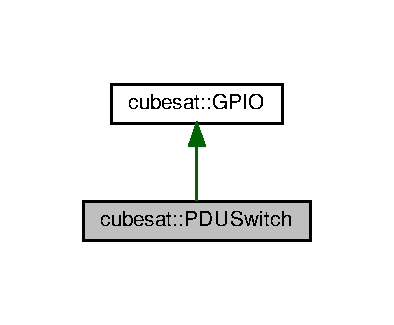
\includegraphics[width=189pt]{classcubesat_1_1PDUSwitch__inherit__graph}
\end{center}
\end{figure}


Collaboration diagram for cubesat\+:\+:P\+D\+U\+Switch\+:\nopagebreak
\begin{figure}[H]
\begin{center}
\leavevmode
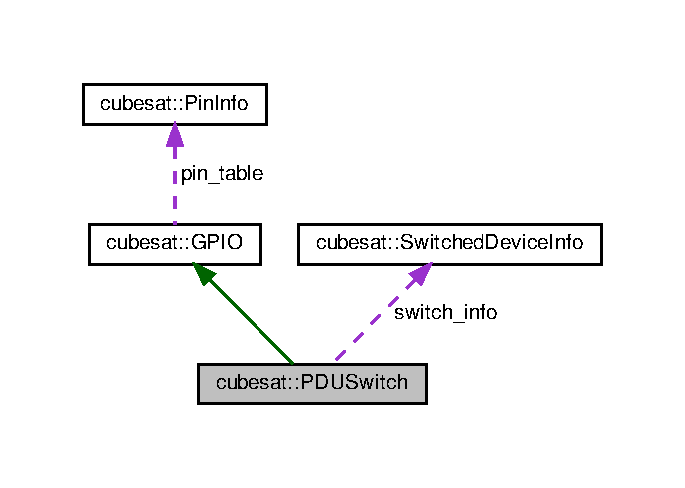
\includegraphics[width=329pt]{classcubesat_1_1PDUSwitch__coll__graph}
\end{center}
\end{figure}
\subsection*{Public Member Functions}
\begin{DoxyCompactItemize}
\item 
\hyperlink{classcubesat_1_1PDUSwitch_a025fa4903a5ae0044948a1c0dc608674}{P\+D\+U\+Switch} (const char $\ast$\hyperlink{classcubesat_1_1PDUSwitch_a2e3a4106c80a9151f795ca3ede55c64f}{name})
\item 
virtual \hyperlink{classcubesat_1_1PDUSwitch_a793dcaa10a20d99985d60d5f432fcbb7}{$\sim$\+P\+D\+U\+Switch} ()
\item 
bool \hyperlink{classcubesat_1_1PDUSwitch_a4312e39a47e11819759e0b0c2d4ab9fe}{Is\+Valid} () const
\item 
\hyperlink{namespacecubesat_a61ab3c9f315851c6eaaf5ad28f97f2e3}{Switch\+State} \hyperlink{classcubesat_1_1PDUSwitch_aca5fd10f2f780e96a5f3cd8601cb21d5}{Set\+State} (\hyperlink{namespacecubesat_a61ab3c9f315851c6eaaf5ad28f97f2e3}{Switch\+State} state)
\begin{DoxyCompactList}\small\item\em Sets the state of the switch. \end{DoxyCompactList}\item 
\hyperlink{namespacecubesat_a61ab3c9f315851c6eaaf5ad28f97f2e3}{Switch\+State} \hyperlink{classcubesat_1_1PDUSwitch_aff0ea06469487418b2fa0e865b74b248}{Get\+State} ()
\begin{DoxyCompactList}\small\item\em Returns the state of the switch. \end{DoxyCompactList}\end{DoxyCompactItemize}
\subsection*{Static Public Member Functions}
\begin{DoxyCompactItemize}
\item 
static const char $\ast$ \hyperlink{classcubesat_1_1PDUSwitch_aa326a238525f39182313fba2dbfb159e}{Get\+Switch\+Name} (\hyperlink{namespacecubesat_a4343cdc3d5f03bad7a16bac6c47cd1ca}{Switch\+ID} \hyperlink{classcubesat_1_1PDUSwitch_a4f528e19179a2a6c07437fc892ca3a73}{switch\+\_\+id})
\item 
static \hyperlink{namespacecubesat_a4343cdc3d5f03bad7a16bac6c47cd1ca}{Switch\+ID} \hyperlink{classcubesat_1_1PDUSwitch_aca06324f41be9ad19fc01dacbbd301e7}{Get\+Switch\+ID} (const char $\ast$switch\+\_\+name)
\item 
static const char $\ast$ \hyperlink{classcubesat_1_1PDUSwitch_a09632cb39b09610b088e3865517d3e4b}{Get\+Switch\+Pin\+Key} (\hyperlink{namespacecubesat_a4343cdc3d5f03bad7a16bac6c47cd1ca}{Switch\+ID} \hyperlink{classcubesat_1_1PDUSwitch_a4f528e19179a2a6c07437fc892ca3a73}{switch\+\_\+id})
\item 
static int \hyperlink{classcubesat_1_1PDUSwitch_a9f3774f4d48d228b066cf441e342661b}{Get\+Switch\+Pin} (\hyperlink{namespacecubesat_a4343cdc3d5f03bad7a16bac6c47cd1ca}{Switch\+ID} \hyperlink{classcubesat_1_1PDUSwitch_a4f528e19179a2a6c07437fc892ca3a73}{switch\+\_\+id})
\item 
static int \hyperlink{classcubesat_1_1PDUSwitch_a8ea76538610e321324eff6bcab2d9ce2}{Get\+Switch\+Pin} (const char $\ast$switch\+\_\+name)
\end{DoxyCompactItemize}
\subsection*{Private Attributes}
\begin{DoxyCompactItemize}
\item 
const char $\ast$ \hyperlink{classcubesat_1_1PDUSwitch_a2e3a4106c80a9151f795ca3ede55c64f}{name}
\item 
\hyperlink{namespacecubesat_a4343cdc3d5f03bad7a16bac6c47cd1ca}{Switch\+ID} \hyperlink{classcubesat_1_1PDUSwitch_a4f528e19179a2a6c07437fc892ca3a73}{switch\+\_\+id}
\end{DoxyCompactItemize}
\subsection*{Static Private Attributes}
\begin{DoxyCompactItemize}
\item 
static \hyperlink{structcubesat_1_1SwitchedDeviceInfo}{Switched\+Device\+Info} \hyperlink{classcubesat_1_1PDUSwitch_ae0f99c4f70fdec9ffca767441bd427db}{switch\+\_\+info} \mbox{[}\hyperlink{switch_8h_ad7db8926cbb872ec36c2e94db869235f}{S\+W\+I\+T\+C\+H\+\_\+\+C\+O\+U\+NT}+1\mbox{]}
\end{DoxyCompactItemize}
\subsection*{Additional Inherited Members}


\subsection{Detailed Description}
A class for controlling the switched lines to the E\+PS. Inherits from the \hyperlink{classcubesat_1_1GPIO}{G\+P\+IO} class. 

\subsection{Constructor \& Destructor Documentation}
\mbox{\Hypertarget{classcubesat_1_1PDUSwitch_a025fa4903a5ae0044948a1c0dc608674}\label{classcubesat_1_1PDUSwitch_a025fa4903a5ae0044948a1c0dc608674}} 
\index{cubesat\+::\+P\+D\+U\+Switch@{cubesat\+::\+P\+D\+U\+Switch}!P\+D\+U\+Switch@{P\+D\+U\+Switch}}
\index{P\+D\+U\+Switch@{P\+D\+U\+Switch}!cubesat\+::\+P\+D\+U\+Switch@{cubesat\+::\+P\+D\+U\+Switch}}
\subsubsection{\texorpdfstring{P\+D\+U\+Switch()}{PDUSwitch()}}
{\footnotesize\ttfamily P\+D\+U\+Switch\+::\+P\+D\+U\+Switch (\begin{DoxyParamCaption}\item[{const char $\ast$}]{name }\end{DoxyParamCaption})}

\mbox{\Hypertarget{classcubesat_1_1PDUSwitch_a793dcaa10a20d99985d60d5f432fcbb7}\label{classcubesat_1_1PDUSwitch_a793dcaa10a20d99985d60d5f432fcbb7}} 
\index{cubesat\+::\+P\+D\+U\+Switch@{cubesat\+::\+P\+D\+U\+Switch}!````~P\+D\+U\+Switch@{$\sim$\+P\+D\+U\+Switch}}
\index{````~P\+D\+U\+Switch@{$\sim$\+P\+D\+U\+Switch}!cubesat\+::\+P\+D\+U\+Switch@{cubesat\+::\+P\+D\+U\+Switch}}
\subsubsection{\texorpdfstring{$\sim$\+P\+D\+U\+Switch()}{~PDUSwitch()}}
{\footnotesize\ttfamily P\+D\+U\+Switch\+::$\sim$\+P\+D\+U\+Switch (\begin{DoxyParamCaption}{ }\end{DoxyParamCaption})\hspace{0.3cm}{\ttfamily [virtual]}}



\subsection{Member Function Documentation}
\mbox{\Hypertarget{classcubesat_1_1PDUSwitch_aff0ea06469487418b2fa0e865b74b248}\label{classcubesat_1_1PDUSwitch_aff0ea06469487418b2fa0e865b74b248}} 
\index{cubesat\+::\+P\+D\+U\+Switch@{cubesat\+::\+P\+D\+U\+Switch}!Get\+State@{Get\+State}}
\index{Get\+State@{Get\+State}!cubesat\+::\+P\+D\+U\+Switch@{cubesat\+::\+P\+D\+U\+Switch}}
\subsubsection{\texorpdfstring{Get\+State()}{GetState()}}
{\footnotesize\ttfamily \hyperlink{namespacecubesat_a61ab3c9f315851c6eaaf5ad28f97f2e3}{Switch\+State} P\+D\+U\+Switch\+::\+Get\+State (\begin{DoxyParamCaption}{ }\end{DoxyParamCaption})}



Returns the state of the switch. 

\begin{DoxyReturn}{Returns}
The state of the switch 
\end{DoxyReturn}
\mbox{\Hypertarget{classcubesat_1_1PDUSwitch_aca06324f41be9ad19fc01dacbbd301e7}\label{classcubesat_1_1PDUSwitch_aca06324f41be9ad19fc01dacbbd301e7}} 
\index{cubesat\+::\+P\+D\+U\+Switch@{cubesat\+::\+P\+D\+U\+Switch}!Get\+Switch\+ID@{Get\+Switch\+ID}}
\index{Get\+Switch\+ID@{Get\+Switch\+ID}!cubesat\+::\+P\+D\+U\+Switch@{cubesat\+::\+P\+D\+U\+Switch}}
\subsubsection{\texorpdfstring{Get\+Switch\+I\+D()}{GetSwitchID()}}
{\footnotesize\ttfamily \hyperlink{namespacecubesat_a4343cdc3d5f03bad7a16bac6c47cd1ca}{Switch\+ID} P\+D\+U\+Switch\+::\+Get\+Switch\+ID (\begin{DoxyParamCaption}\item[{const char $\ast$}]{switch\+\_\+name }\end{DoxyParamCaption})\hspace{0.3cm}{\ttfamily [static]}}

\mbox{\Hypertarget{classcubesat_1_1PDUSwitch_aa326a238525f39182313fba2dbfb159e}\label{classcubesat_1_1PDUSwitch_aa326a238525f39182313fba2dbfb159e}} 
\index{cubesat\+::\+P\+D\+U\+Switch@{cubesat\+::\+P\+D\+U\+Switch}!Get\+Switch\+Name@{Get\+Switch\+Name}}
\index{Get\+Switch\+Name@{Get\+Switch\+Name}!cubesat\+::\+P\+D\+U\+Switch@{cubesat\+::\+P\+D\+U\+Switch}}
\subsubsection{\texorpdfstring{Get\+Switch\+Name()}{GetSwitchName()}}
{\footnotesize\ttfamily const char $\ast$ P\+D\+U\+Switch\+::\+Get\+Switch\+Name (\begin{DoxyParamCaption}\item[{\hyperlink{namespacecubesat_a4343cdc3d5f03bad7a16bac6c47cd1ca}{Switch\+ID}}]{switch\+\_\+id }\end{DoxyParamCaption})\hspace{0.3cm}{\ttfamily [static]}}

\mbox{\Hypertarget{classcubesat_1_1PDUSwitch_a9f3774f4d48d228b066cf441e342661b}\label{classcubesat_1_1PDUSwitch_a9f3774f4d48d228b066cf441e342661b}} 
\index{cubesat\+::\+P\+D\+U\+Switch@{cubesat\+::\+P\+D\+U\+Switch}!Get\+Switch\+Pin@{Get\+Switch\+Pin}}
\index{Get\+Switch\+Pin@{Get\+Switch\+Pin}!cubesat\+::\+P\+D\+U\+Switch@{cubesat\+::\+P\+D\+U\+Switch}}
\subsubsection{\texorpdfstring{Get\+Switch\+Pin()}{GetSwitchPin()}\hspace{0.1cm}{\footnotesize\ttfamily [1/2]}}
{\footnotesize\ttfamily int P\+D\+U\+Switch\+::\+Get\+Switch\+Pin (\begin{DoxyParamCaption}\item[{\hyperlink{namespacecubesat_a4343cdc3d5f03bad7a16bac6c47cd1ca}{Switch\+ID}}]{switch\+\_\+id }\end{DoxyParamCaption})\hspace{0.3cm}{\ttfamily [static]}}

\mbox{\Hypertarget{classcubesat_1_1PDUSwitch_a8ea76538610e321324eff6bcab2d9ce2}\label{classcubesat_1_1PDUSwitch_a8ea76538610e321324eff6bcab2d9ce2}} 
\index{cubesat\+::\+P\+D\+U\+Switch@{cubesat\+::\+P\+D\+U\+Switch}!Get\+Switch\+Pin@{Get\+Switch\+Pin}}
\index{Get\+Switch\+Pin@{Get\+Switch\+Pin}!cubesat\+::\+P\+D\+U\+Switch@{cubesat\+::\+P\+D\+U\+Switch}}
\subsubsection{\texorpdfstring{Get\+Switch\+Pin()}{GetSwitchPin()}\hspace{0.1cm}{\footnotesize\ttfamily [2/2]}}
{\footnotesize\ttfamily int P\+D\+U\+Switch\+::\+Get\+Switch\+Pin (\begin{DoxyParamCaption}\item[{const char $\ast$}]{switch\+\_\+name }\end{DoxyParamCaption})\hspace{0.3cm}{\ttfamily [static]}}

\mbox{\Hypertarget{classcubesat_1_1PDUSwitch_a09632cb39b09610b088e3865517d3e4b}\label{classcubesat_1_1PDUSwitch_a09632cb39b09610b088e3865517d3e4b}} 
\index{cubesat\+::\+P\+D\+U\+Switch@{cubesat\+::\+P\+D\+U\+Switch}!Get\+Switch\+Pin\+Key@{Get\+Switch\+Pin\+Key}}
\index{Get\+Switch\+Pin\+Key@{Get\+Switch\+Pin\+Key}!cubesat\+::\+P\+D\+U\+Switch@{cubesat\+::\+P\+D\+U\+Switch}}
\subsubsection{\texorpdfstring{Get\+Switch\+Pin\+Key()}{GetSwitchPinKey()}}
{\footnotesize\ttfamily const char $\ast$ P\+D\+U\+Switch\+::\+Get\+Switch\+Pin\+Key (\begin{DoxyParamCaption}\item[{\hyperlink{namespacecubesat_a4343cdc3d5f03bad7a16bac6c47cd1ca}{Switch\+ID}}]{switch\+\_\+id }\end{DoxyParamCaption})\hspace{0.3cm}{\ttfamily [static]}}

\mbox{\Hypertarget{classcubesat_1_1PDUSwitch_a4312e39a47e11819759e0b0c2d4ab9fe}\label{classcubesat_1_1PDUSwitch_a4312e39a47e11819759e0b0c2d4ab9fe}} 
\index{cubesat\+::\+P\+D\+U\+Switch@{cubesat\+::\+P\+D\+U\+Switch}!Is\+Valid@{Is\+Valid}}
\index{Is\+Valid@{Is\+Valid}!cubesat\+::\+P\+D\+U\+Switch@{cubesat\+::\+P\+D\+U\+Switch}}
\subsubsection{\texorpdfstring{Is\+Valid()}{IsValid()}}
{\footnotesize\ttfamily bool cubesat\+::\+P\+D\+U\+Switch\+::\+Is\+Valid (\begin{DoxyParamCaption}{ }\end{DoxyParamCaption}) const\hspace{0.3cm}{\ttfamily [inline]}}

\mbox{\Hypertarget{classcubesat_1_1PDUSwitch_aca5fd10f2f780e96a5f3cd8601cb21d5}\label{classcubesat_1_1PDUSwitch_aca5fd10f2f780e96a5f3cd8601cb21d5}} 
\index{cubesat\+::\+P\+D\+U\+Switch@{cubesat\+::\+P\+D\+U\+Switch}!Set\+State@{Set\+State}}
\index{Set\+State@{Set\+State}!cubesat\+::\+P\+D\+U\+Switch@{cubesat\+::\+P\+D\+U\+Switch}}
\subsubsection{\texorpdfstring{Set\+State()}{SetState()}}
{\footnotesize\ttfamily \hyperlink{namespacecubesat_a61ab3c9f315851c6eaaf5ad28f97f2e3}{Switch\+State} P\+D\+U\+Switch\+::\+Set\+State (\begin{DoxyParamCaption}\item[{\hyperlink{namespacecubesat_a61ab3c9f315851c6eaaf5ad28f97f2e3}{Switch\+State}}]{state }\end{DoxyParamCaption})}



Sets the state of the switch. 


\begin{DoxyParams}{Parameters}
{\em state} & The state of the switch \\
\hline
\end{DoxyParams}
\begin{DoxyReturn}{Returns}
The state the switch was set to 
\end{DoxyReturn}


\subsection{Member Data Documentation}
\mbox{\Hypertarget{classcubesat_1_1PDUSwitch_a2e3a4106c80a9151f795ca3ede55c64f}\label{classcubesat_1_1PDUSwitch_a2e3a4106c80a9151f795ca3ede55c64f}} 
\index{cubesat\+::\+P\+D\+U\+Switch@{cubesat\+::\+P\+D\+U\+Switch}!name@{name}}
\index{name@{name}!cubesat\+::\+P\+D\+U\+Switch@{cubesat\+::\+P\+D\+U\+Switch}}
\subsubsection{\texorpdfstring{name}{name}}
{\footnotesize\ttfamily const char$\ast$ cubesat\+::\+P\+D\+U\+Switch\+::name\hspace{0.3cm}{\ttfamily [private]}}

\mbox{\Hypertarget{classcubesat_1_1PDUSwitch_a4f528e19179a2a6c07437fc892ca3a73}\label{classcubesat_1_1PDUSwitch_a4f528e19179a2a6c07437fc892ca3a73}} 
\index{cubesat\+::\+P\+D\+U\+Switch@{cubesat\+::\+P\+D\+U\+Switch}!switch\+\_\+id@{switch\+\_\+id}}
\index{switch\+\_\+id@{switch\+\_\+id}!cubesat\+::\+P\+D\+U\+Switch@{cubesat\+::\+P\+D\+U\+Switch}}
\subsubsection{\texorpdfstring{switch\+\_\+id}{switch\_id}}
{\footnotesize\ttfamily \hyperlink{namespacecubesat_a4343cdc3d5f03bad7a16bac6c47cd1ca}{Switch\+ID} cubesat\+::\+P\+D\+U\+Switch\+::switch\+\_\+id\hspace{0.3cm}{\ttfamily [private]}}

\mbox{\Hypertarget{classcubesat_1_1PDUSwitch_ae0f99c4f70fdec9ffca767441bd427db}\label{classcubesat_1_1PDUSwitch_ae0f99c4f70fdec9ffca767441bd427db}} 
\index{cubesat\+::\+P\+D\+U\+Switch@{cubesat\+::\+P\+D\+U\+Switch}!switch\+\_\+info@{switch\+\_\+info}}
\index{switch\+\_\+info@{switch\+\_\+info}!cubesat\+::\+P\+D\+U\+Switch@{cubesat\+::\+P\+D\+U\+Switch}}
\subsubsection{\texorpdfstring{switch\+\_\+info}{switch\_info}}
{\footnotesize\ttfamily \hyperlink{structcubesat_1_1SwitchedDeviceInfo}{Switched\+Device\+Info} P\+D\+U\+Switch\+::switch\+\_\+info\hspace{0.3cm}{\ttfamily [static]}, {\ttfamily [private]}}

{\bfseries Initial value\+:}
\begin{DoxyCode}
= \{
    \{\hyperlink{switch_8h_a128560820edeca7416767b0278974f97}{SWITCH\_HEATER\_NAME}, \hyperlink{switch_8h_ac4a41c3b8145477d4d658f975adfc5de}{SWITCH\_HEATER\_KEY}\},
    \{\hyperlink{switch_8h_ab87f0daf3c993cbb43485e40fd11a584}{SWITCH\_TEMPSENSOR\_NAME}, \hyperlink{switch_8h_a34ce8812e308ab41e84a54561ab5e29d}{SWITCH\_TEMPSENSOR\_KEY}\},
    \{\hyperlink{switch_8h_a079b325f48bc449963b8f5c0b84c1455}{SWITCH\_SUNSENSOR\_NAME}, \hyperlink{switch_8h_a0e876cac82ae0ac174eb90ee8f919288}{SWITCH\_SUNSENSOR\_KEY}\},
    \{NULL, NULL\}
\}
\end{DoxyCode}


The documentation for this class was generated from the following files\+:\begin{DoxyCompactItemize}
\item 
/home/osboxes/cosmos/source/projects/cubesat-\/kit/include/device/\hyperlink{switch_8h}{switch.\+h}\item 
/home/osboxes/cosmos/source/projects/cubesat-\/kit/source/device/\hyperlink{switch_8cpp}{switch.\+cpp}\end{DoxyCompactItemize}

\hypertarget{structcubesat_1_1PinInfo}{}\section{cubesat\+:\+:Pin\+Info Struct Reference}
\label{structcubesat_1_1PinInfo}\index{cubesat\+::\+Pin\+Info@{cubesat\+::\+Pin\+Info}}


{\ttfamily \#include $<$G\+P\+I\+O.\+h$>$}

\subsection*{Public Attributes}
\begin{DoxyCompactItemize}
\item 
const char $\ast$ \hyperlink{structcubesat_1_1PinInfo_aa3d90d09c4265b07b2fe523300d89d2b}{name}
\item 
const char $\ast$ \hyperlink{structcubesat_1_1PinInfo_a5336be9370a0ae23256fbe715217dc9b}{key}
\item 
\hyperlink{namespacecubesat_af928ed4b56ef60d75953a91225b37a00}{Pin} \hyperlink{structcubesat_1_1PinInfo_ab81fbc40928199ff436a40b58e780ce4}{gpio}
\item 
int \hyperlink{structcubesat_1_1PinInfo_a7f8c9d7e69fea74ccec40ed3cbbbac4b}{pwm\+\_\+mux\+\_\+mode}
\item 
int \hyperlink{structcubesat_1_1PinInfo_aeae977c2657f5e26cd112272255ef276}{ain}
\item 
int \hyperlink{structcubesat_1_1PinInfo_aab65aaa102e8b854c5f928f1adb30a37}{is\+Allocated\+By\+Default}
\end{DoxyCompactItemize}


\subsection{Member Data Documentation}
\mbox{\Hypertarget{structcubesat_1_1PinInfo_aeae977c2657f5e26cd112272255ef276}\label{structcubesat_1_1PinInfo_aeae977c2657f5e26cd112272255ef276}} 
\index{cubesat\+::\+Pin\+Info@{cubesat\+::\+Pin\+Info}!ain@{ain}}
\index{ain@{ain}!cubesat\+::\+Pin\+Info@{cubesat\+::\+Pin\+Info}}
\subsubsection{\texorpdfstring{ain}{ain}}
{\footnotesize\ttfamily int cubesat\+::\+Pin\+Info\+::ain}

\mbox{\Hypertarget{structcubesat_1_1PinInfo_ab81fbc40928199ff436a40b58e780ce4}\label{structcubesat_1_1PinInfo_ab81fbc40928199ff436a40b58e780ce4}} 
\index{cubesat\+::\+Pin\+Info@{cubesat\+::\+Pin\+Info}!gpio@{gpio}}
\index{gpio@{gpio}!cubesat\+::\+Pin\+Info@{cubesat\+::\+Pin\+Info}}
\subsubsection{\texorpdfstring{gpio}{gpio}}
{\footnotesize\ttfamily \hyperlink{namespacecubesat_af928ed4b56ef60d75953a91225b37a00}{Pin} cubesat\+::\+Pin\+Info\+::gpio}

\mbox{\Hypertarget{structcubesat_1_1PinInfo_aab65aaa102e8b854c5f928f1adb30a37}\label{structcubesat_1_1PinInfo_aab65aaa102e8b854c5f928f1adb30a37}} 
\index{cubesat\+::\+Pin\+Info@{cubesat\+::\+Pin\+Info}!is\+Allocated\+By\+Default@{is\+Allocated\+By\+Default}}
\index{is\+Allocated\+By\+Default@{is\+Allocated\+By\+Default}!cubesat\+::\+Pin\+Info@{cubesat\+::\+Pin\+Info}}
\subsubsection{\texorpdfstring{is\+Allocated\+By\+Default}{isAllocatedByDefault}}
{\footnotesize\ttfamily int cubesat\+::\+Pin\+Info\+::is\+Allocated\+By\+Default}

\mbox{\Hypertarget{structcubesat_1_1PinInfo_a5336be9370a0ae23256fbe715217dc9b}\label{structcubesat_1_1PinInfo_a5336be9370a0ae23256fbe715217dc9b}} 
\index{cubesat\+::\+Pin\+Info@{cubesat\+::\+Pin\+Info}!key@{key}}
\index{key@{key}!cubesat\+::\+Pin\+Info@{cubesat\+::\+Pin\+Info}}
\subsubsection{\texorpdfstring{key}{key}}
{\footnotesize\ttfamily const char$\ast$ cubesat\+::\+Pin\+Info\+::key}

\mbox{\Hypertarget{structcubesat_1_1PinInfo_aa3d90d09c4265b07b2fe523300d89d2b}\label{structcubesat_1_1PinInfo_aa3d90d09c4265b07b2fe523300d89d2b}} 
\index{cubesat\+::\+Pin\+Info@{cubesat\+::\+Pin\+Info}!name@{name}}
\index{name@{name}!cubesat\+::\+Pin\+Info@{cubesat\+::\+Pin\+Info}}
\subsubsection{\texorpdfstring{name}{name}}
{\footnotesize\ttfamily const char$\ast$ cubesat\+::\+Pin\+Info\+::name}

\mbox{\Hypertarget{structcubesat_1_1PinInfo_a7f8c9d7e69fea74ccec40ed3cbbbac4b}\label{structcubesat_1_1PinInfo_a7f8c9d7e69fea74ccec40ed3cbbbac4b}} 
\index{cubesat\+::\+Pin\+Info@{cubesat\+::\+Pin\+Info}!pwm\+\_\+mux\+\_\+mode@{pwm\+\_\+mux\+\_\+mode}}
\index{pwm\+\_\+mux\+\_\+mode@{pwm\+\_\+mux\+\_\+mode}!cubesat\+::\+Pin\+Info@{cubesat\+::\+Pin\+Info}}
\subsubsection{\texorpdfstring{pwm\+\_\+mux\+\_\+mode}{pwm\_mux\_mode}}
{\footnotesize\ttfamily int cubesat\+::\+Pin\+Info\+::pwm\+\_\+mux\+\_\+mode}



The documentation for this struct was generated from the following file\+:\begin{DoxyCompactItemize}
\item 
/home/osboxes/cosmos/source/projects/cubesat-\/kit/include/device/\hyperlink{GPIO_8h}{G\+P\+I\+O.\+h}\end{DoxyCompactItemize}

\hypertarget{structcubesat_1_1Device_1_1PostedProperty}{}\section{cubesat\+:\+:Device\+:\+:Posted\+Property Struct Reference}
\label{structcubesat_1_1Device_1_1PostedProperty}\index{cubesat\+::\+Device\+::\+Posted\+Property@{cubesat\+::\+Device\+::\+Posted\+Property}}
\subsection*{Public Attributes}
\begin{DoxyCompactItemize}
\item 
std\+::string \hyperlink{structcubesat_1_1Device_1_1PostedProperty_a566da00f8a06588980f3661bc7ab0442}{readable\+\_\+name}
\item 
std\+::string \hyperlink{structcubesat_1_1Device_1_1PostedProperty_a8bc44aa9e44c60a7d6371325de7ac285}{cosmos\+\_\+name}
\end{DoxyCompactItemize}


\subsection{Member Data Documentation}
\mbox{\Hypertarget{structcubesat_1_1Device_1_1PostedProperty_a8bc44aa9e44c60a7d6371325de7ac285}\label{structcubesat_1_1Device_1_1PostedProperty_a8bc44aa9e44c60a7d6371325de7ac285}} 
\index{cubesat\+::\+Device\+::\+Posted\+Property@{cubesat\+::\+Device\+::\+Posted\+Property}!cosmos\+\_\+name@{cosmos\+\_\+name}}
\index{cosmos\+\_\+name@{cosmos\+\_\+name}!cubesat\+::\+Device\+::\+Posted\+Property@{cubesat\+::\+Device\+::\+Posted\+Property}}
\subsubsection{\texorpdfstring{cosmos\+\_\+name}{cosmos\_name}}
{\footnotesize\ttfamily std\+::string cubesat\+::\+Device\+::\+Posted\+Property\+::cosmos\+\_\+name}

\mbox{\Hypertarget{structcubesat_1_1Device_1_1PostedProperty_a566da00f8a06588980f3661bc7ab0442}\label{structcubesat_1_1Device_1_1PostedProperty_a566da00f8a06588980f3661bc7ab0442}} 
\index{cubesat\+::\+Device\+::\+Posted\+Property@{cubesat\+::\+Device\+::\+Posted\+Property}!readable\+\_\+name@{readable\+\_\+name}}
\index{readable\+\_\+name@{readable\+\_\+name}!cubesat\+::\+Device\+::\+Posted\+Property@{cubesat\+::\+Device\+::\+Posted\+Property}}
\subsubsection{\texorpdfstring{readable\+\_\+name}{readable\_name}}
{\footnotesize\ttfamily std\+::string cubesat\+::\+Device\+::\+Posted\+Property\+::readable\+\_\+name}



The documentation for this struct was generated from the following file\+:\begin{DoxyCompactItemize}
\item 
/home/osboxes/cosmos/source/projects/cubesat-\/kit/include/utility/\hyperlink{Device_8h}{Device.\+h}\end{DoxyCompactItemize}

\hypertarget{structcubesat_1_1Node_1_1PowerGeneration}{}\section{cubesat\+:\+:Node\+:\+:Power\+Generation Struct Reference}
\label{structcubesat_1_1Node_1_1PowerGeneration}\index{cubesat\+::\+Node\+::\+Power\+Generation@{cubesat\+::\+Node\+::\+Power\+Generation}}


{\ttfamily \#include $<$Device\+Detail.\+h$>$}



Inheritance diagram for cubesat\+:\+:Node\+:\+:Power\+Generation\+:
\nopagebreak
\begin{figure}[H]
\begin{center}
\leavevmode
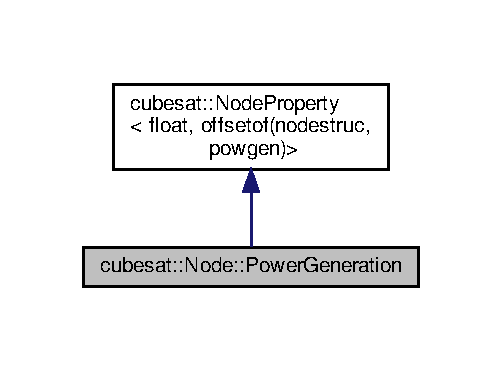
\includegraphics[width=241pt]{structcubesat_1_1Node_1_1PowerGeneration__inherit__graph}
\end{center}
\end{figure}


Collaboration diagram for cubesat\+:\+:Node\+:\+:Power\+Generation\+:
\nopagebreak
\begin{figure}[H]
\begin{center}
\leavevmode
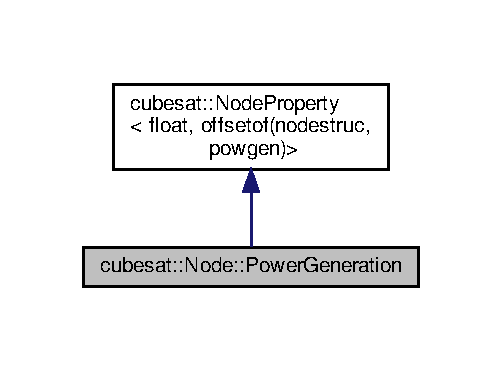
\includegraphics[width=241pt]{structcubesat_1_1Node_1_1PowerGeneration__coll__graph}
\end{center}
\end{figure}
\subsection*{Static Public Attributes}
\begin{DoxyCompactItemize}
\item 
static constexpr auto \hyperlink{structcubesat_1_1Node_1_1PowerGeneration_af48c2b095fe2982e99d16e3c291ccc87}{key} = \char`\"{}node\+\_\+powgen\char`\"{}
\item 
static constexpr const char $\ast$ \hyperlink{structcubesat_1_1Node_1_1PowerGeneration_a076b9debf2e98be02ead5aae6d5f23f2}{name} = \char`\"{}Power Generation\char`\"{}
\end{DoxyCompactItemize}
\subsection*{Additional Inherited Members}


\subsection{Member Data Documentation}
\mbox{\Hypertarget{structcubesat_1_1Node_1_1PowerGeneration_af48c2b095fe2982e99d16e3c291ccc87}\label{structcubesat_1_1Node_1_1PowerGeneration_af48c2b095fe2982e99d16e3c291ccc87}} 
\index{cubesat\+::\+Node\+::\+Power\+Generation@{cubesat\+::\+Node\+::\+Power\+Generation}!key@{key}}
\index{key@{key}!cubesat\+::\+Node\+::\+Power\+Generation@{cubesat\+::\+Node\+::\+Power\+Generation}}
\subsubsection{\texorpdfstring{key}{key}}
{\footnotesize\ttfamily constexpr auto cubesat\+::\+Node\+::\+Power\+Generation\+::key = \char`\"{}node\+\_\+powgen\char`\"{}\hspace{0.3cm}{\ttfamily [static]}}

\mbox{\Hypertarget{structcubesat_1_1Node_1_1PowerGeneration_a076b9debf2e98be02ead5aae6d5f23f2}\label{structcubesat_1_1Node_1_1PowerGeneration_a076b9debf2e98be02ead5aae6d5f23f2}} 
\index{cubesat\+::\+Node\+::\+Power\+Generation@{cubesat\+::\+Node\+::\+Power\+Generation}!name@{name}}
\index{name@{name}!cubesat\+::\+Node\+::\+Power\+Generation@{cubesat\+::\+Node\+::\+Power\+Generation}}
\subsubsection{\texorpdfstring{name}{name}}
{\footnotesize\ttfamily constexpr const char$\ast$ cubesat\+::\+Node\+::\+Power\+Generation\+::name = \char`\"{}Power Generation\char`\"{}\hspace{0.3cm}{\ttfamily [static]}}



The documentation for this struct was generated from the following file\+:\begin{DoxyCompactItemize}
\item 
/home/osboxes/cosmos/source/projects/cubesat-\/kit/include/utility/\hyperlink{DeviceDetail_8h}{Device\+Detail.\+h}\end{DoxyCompactItemize}

\hypertarget{structcubesat_1_1Node_1_1PowerUse}{}\section{cubesat\+:\+:Node\+:\+:Power\+Use Struct Reference}
\label{structcubesat_1_1Node_1_1PowerUse}\index{cubesat\+::\+Node\+::\+Power\+Use@{cubesat\+::\+Node\+::\+Power\+Use}}


{\ttfamily \#include $<$Device\+Detail.\+h$>$}



Inheritance diagram for cubesat\+:\+:Node\+:\+:Power\+Use\+:
\nopagebreak
\begin{figure}[H]
\begin{center}
\leavevmode
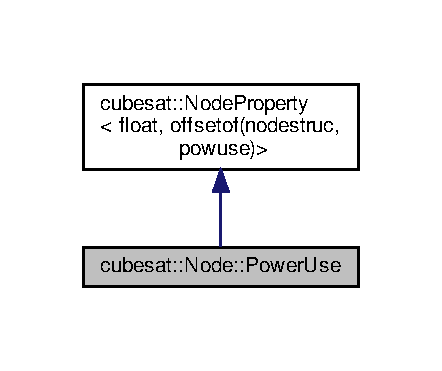
\includegraphics[width=212pt]{structcubesat_1_1Node_1_1PowerUse__inherit__graph}
\end{center}
\end{figure}


Collaboration diagram for cubesat\+:\+:Node\+:\+:Power\+Use\+:
\nopagebreak
\begin{figure}[H]
\begin{center}
\leavevmode
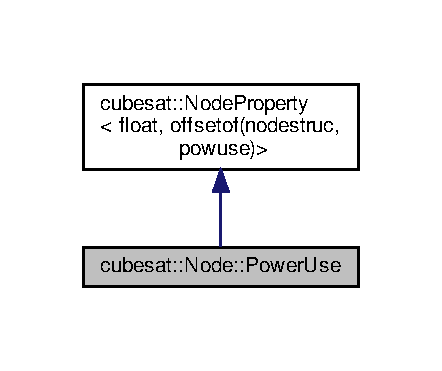
\includegraphics[width=212pt]{structcubesat_1_1Node_1_1PowerUse__coll__graph}
\end{center}
\end{figure}
\subsection*{Static Public Attributes}
\begin{DoxyCompactItemize}
\item 
static constexpr auto \hyperlink{structcubesat_1_1Node_1_1PowerUse_ab7c371f173e9a45244ebf968353f0950}{key} = \char`\"{}node\+\_\+powuse\char`\"{}
\item 
static constexpr const char $\ast$ \hyperlink{structcubesat_1_1Node_1_1PowerUse_a585c9a22ac829b783f35656c4d9a7df6}{name} = \char`\"{}Power Use\char`\"{}
\end{DoxyCompactItemize}
\subsection*{Additional Inherited Members}


\subsection{Member Data Documentation}
\mbox{\Hypertarget{structcubesat_1_1Node_1_1PowerUse_ab7c371f173e9a45244ebf968353f0950}\label{structcubesat_1_1Node_1_1PowerUse_ab7c371f173e9a45244ebf968353f0950}} 
\index{cubesat\+::\+Node\+::\+Power\+Use@{cubesat\+::\+Node\+::\+Power\+Use}!key@{key}}
\index{key@{key}!cubesat\+::\+Node\+::\+Power\+Use@{cubesat\+::\+Node\+::\+Power\+Use}}
\subsubsection{\texorpdfstring{key}{key}}
{\footnotesize\ttfamily constexpr auto cubesat\+::\+Node\+::\+Power\+Use\+::key = \char`\"{}node\+\_\+powuse\char`\"{}\hspace{0.3cm}{\ttfamily [static]}}

\mbox{\Hypertarget{structcubesat_1_1Node_1_1PowerUse_a585c9a22ac829b783f35656c4d9a7df6}\label{structcubesat_1_1Node_1_1PowerUse_a585c9a22ac829b783f35656c4d9a7df6}} 
\index{cubesat\+::\+Node\+::\+Power\+Use@{cubesat\+::\+Node\+::\+Power\+Use}!name@{name}}
\index{name@{name}!cubesat\+::\+Node\+::\+Power\+Use@{cubesat\+::\+Node\+::\+Power\+Use}}
\subsubsection{\texorpdfstring{name}{name}}
{\footnotesize\ttfamily constexpr const char$\ast$ cubesat\+::\+Node\+::\+Power\+Use\+::name = \char`\"{}Power Use\char`\"{}\hspace{0.3cm}{\ttfamily [static]}}



The documentation for this struct was generated from the following file\+:\begin{DoxyCompactItemize}
\item 
/home/osboxes/cosmos/source/projects/cubesat-\/kit/include/utility/\hyperlink{DeviceDetail_8h}{Device\+Detail.\+h}\end{DoxyCompactItemize}

\hypertarget{structcubesat_1_1Property}{}\section{cubesat\+:\+:Property$<$ device\+\_\+struc, offset $>$ Struct Template Reference}
\label{structcubesat_1_1Property}\index{cubesat\+::\+Property$<$ device\+\_\+struc, offset $>$@{cubesat\+::\+Property$<$ device\+\_\+struc, offset $>$}}


{\ttfamily \#include $<$Device\+Detail.\+h$>$}

\subsection*{Public Types}
\begin{DoxyCompactItemize}
\item 
using \hyperlink{structcubesat_1_1Property_abde80e33ecde1656ac9035d4b52477ce}{Meta\+Data} = \hyperlink{structcubesat_1_1PropertyMeta}{Property\+Meta}$<$ device\+\_\+struc, offset $>$
\begin{DoxyCompactList}\small\item\em The \hyperlink{structcubesat_1_1PropertyMeta}{Property\+Meta} type for this property. \end{DoxyCompactList}\item 
using \hyperlink{structcubesat_1_1Property_a01cc6c681c8f3dcb97f16d186a04ca73}{Member\+Type} = typename \hyperlink{structcubesat_1_1PropertyMeta}{Property\+Meta}$<$ device\+\_\+struc, offset $>$\+::\hyperlink{structcubesat_1_1Property_a01cc6c681c8f3dcb97f16d186a04ca73}{Member\+Type}
\begin{DoxyCompactList}\small\item\em The actual member type used in the device\+\_\+struc declaration. \end{DoxyCompactList}\item 
using \hyperlink{structcubesat_1_1Property_a24aaec6241faac15f50c63bb6c972fd4}{Value\+Type} = typename \hyperlink{structcubesat_1_1PropertyMeta}{Property\+Meta}$<$ device\+\_\+struc, offset $>$\+::\hyperlink{structcubesat_1_1Property_a24aaec6241faac15f50c63bb6c972fd4}{Value\+Type}
\begin{DoxyCompactList}\small\item\em The value type expected (may or may not be the same as the Member\+Type) \end{DoxyCompactList}\end{DoxyCompactItemize}
\subsection*{Public Member Functions}
\begin{DoxyCompactItemize}
\item 
\hyperlink{structcubesat_1_1Property_a12f691402fdf35461ddad1c88a6142d8}{Property} (Agent $\ast$\hyperlink{structcubesat_1_1Property_a04415356b5a01900753d1fb26987ace8}{agent}, int \hyperlink{structcubesat_1_1Property_a69c661b3e78deee31af23956fc6130c5}{cindex})
\item 
\hyperlink{structcubesat_1_1Property}{Property} \& \hyperlink{structcubesat_1_1Property_a5aa93e37bf7adaa56ac3a9fba407e12c}{operator=} (\hyperlink{structcubesat_1_1Property_a24aaec6241faac15f50c63bb6c972fd4}{Value\+Type} value)
\begin{DoxyCompactList}\small\item\em Stores the given value in the C\+O\+S\+M\+OS namespace. \end{DoxyCompactList}\item 
\hyperlink{structcubesat_1_1Property_ac8aa543ac4a3ea760a2291ad408b34ff}{operator Value\+Type} ()
\begin{DoxyCompactList}\small\item\em Retrieves the value in the C\+O\+S\+M\+OS namespace. \end{DoxyCompactList}\end{DoxyCompactItemize}
\subsection*{Private Attributes}
\begin{DoxyCompactItemize}
\item 
Agent $\ast$ \hyperlink{structcubesat_1_1Property_a04415356b5a01900753d1fb26987ace8}{agent}
\begin{DoxyCompactList}\small\item\em The agent used to access the C\+O\+S\+M\+OS namespace. \end{DoxyCompactList}\item 
int \hyperlink{structcubesat_1_1Property_a69c661b3e78deee31af23956fc6130c5}{cindex}
\begin{DoxyCompactList}\small\item\em The component index of the device this property belongs to. \end{DoxyCompactList}\end{DoxyCompactItemize}


\subsection{Member Typedef Documentation}
\mbox{\Hypertarget{structcubesat_1_1Property_a01cc6c681c8f3dcb97f16d186a04ca73}\label{structcubesat_1_1Property_a01cc6c681c8f3dcb97f16d186a04ca73}} 
\index{cubesat\+::\+Property@{cubesat\+::\+Property}!Member\+Type@{Member\+Type}}
\index{Member\+Type@{Member\+Type}!cubesat\+::\+Property@{cubesat\+::\+Property}}
\subsubsection{\texorpdfstring{Member\+Type}{MemberType}}
{\footnotesize\ttfamily template$<$typename device\+\_\+struc , size\+\_\+t offset$>$ \\
using \hyperlink{structcubesat_1_1Property}{cubesat\+::\+Property}$<$ device\+\_\+struc, offset $>$\+::\hyperlink{structcubesat_1_1Property_a01cc6c681c8f3dcb97f16d186a04ca73}{Member\+Type} =  typename \hyperlink{structcubesat_1_1PropertyMeta}{Property\+Meta}$<$device\+\_\+struc, offset$>$\+::\hyperlink{structcubesat_1_1Property_a01cc6c681c8f3dcb97f16d186a04ca73}{Member\+Type}}



The actual member type used in the device\+\_\+struc declaration. 

\mbox{\Hypertarget{structcubesat_1_1Property_abde80e33ecde1656ac9035d4b52477ce}\label{structcubesat_1_1Property_abde80e33ecde1656ac9035d4b52477ce}} 
\index{cubesat\+::\+Property@{cubesat\+::\+Property}!Meta\+Data@{Meta\+Data}}
\index{Meta\+Data@{Meta\+Data}!cubesat\+::\+Property@{cubesat\+::\+Property}}
\subsubsection{\texorpdfstring{Meta\+Data}{MetaData}}
{\footnotesize\ttfamily template$<$typename device\+\_\+struc , size\+\_\+t offset$>$ \\
using \hyperlink{structcubesat_1_1Property}{cubesat\+::\+Property}$<$ device\+\_\+struc, offset $>$\+::\hyperlink{structcubesat_1_1Property_abde80e33ecde1656ac9035d4b52477ce}{Meta\+Data} =  \hyperlink{structcubesat_1_1PropertyMeta}{Property\+Meta}$<$device\+\_\+struc, offset$>$}



The \hyperlink{structcubesat_1_1PropertyMeta}{Property\+Meta} type for this property. 

\mbox{\Hypertarget{structcubesat_1_1Property_a24aaec6241faac15f50c63bb6c972fd4}\label{structcubesat_1_1Property_a24aaec6241faac15f50c63bb6c972fd4}} 
\index{cubesat\+::\+Property@{cubesat\+::\+Property}!Value\+Type@{Value\+Type}}
\index{Value\+Type@{Value\+Type}!cubesat\+::\+Property@{cubesat\+::\+Property}}
\subsubsection{\texorpdfstring{Value\+Type}{ValueType}}
{\footnotesize\ttfamily template$<$typename device\+\_\+struc , size\+\_\+t offset$>$ \\
using \hyperlink{structcubesat_1_1Property}{cubesat\+::\+Property}$<$ device\+\_\+struc, offset $>$\+::\hyperlink{structcubesat_1_1Property_a24aaec6241faac15f50c63bb6c972fd4}{Value\+Type} =  typename \hyperlink{structcubesat_1_1PropertyMeta}{Property\+Meta}$<$device\+\_\+struc, offset$>$\+::\hyperlink{structcubesat_1_1Property_a24aaec6241faac15f50c63bb6c972fd4}{Value\+Type}}



The value type expected (may or may not be the same as the Member\+Type) 



\subsection{Constructor \& Destructor Documentation}
\mbox{\Hypertarget{structcubesat_1_1Property_a12f691402fdf35461ddad1c88a6142d8}\label{structcubesat_1_1Property_a12f691402fdf35461ddad1c88a6142d8}} 
\index{cubesat\+::\+Property@{cubesat\+::\+Property}!Property@{Property}}
\index{Property@{Property}!cubesat\+::\+Property@{cubesat\+::\+Property}}
\subsubsection{\texorpdfstring{Property()}{Property()}}
{\footnotesize\ttfamily template$<$typename device\+\_\+struc , size\+\_\+t offset$>$ \\
\hyperlink{structcubesat_1_1Property}{cubesat\+::\+Property}$<$ device\+\_\+struc, offset $>$\+::\hyperlink{structcubesat_1_1Property}{Property} (\begin{DoxyParamCaption}\item[{Agent $\ast$}]{agent,  }\item[{int}]{cindex }\end{DoxyParamCaption})\hspace{0.3cm}{\ttfamily [inline]}}



\subsection{Member Function Documentation}
\mbox{\Hypertarget{structcubesat_1_1Property_ac8aa543ac4a3ea760a2291ad408b34ff}\label{structcubesat_1_1Property_ac8aa543ac4a3ea760a2291ad408b34ff}} 
\index{cubesat\+::\+Property@{cubesat\+::\+Property}!operator Value\+Type@{operator Value\+Type}}
\index{operator Value\+Type@{operator Value\+Type}!cubesat\+::\+Property@{cubesat\+::\+Property}}
\subsubsection{\texorpdfstring{operator Value\+Type()}{operator ValueType()}}
{\footnotesize\ttfamily template$<$typename device\+\_\+struc , size\+\_\+t offset$>$ \\
\hyperlink{structcubesat_1_1Property}{cubesat\+::\+Property}$<$ device\+\_\+struc, offset $>$\+::operator \hyperlink{structcubesat_1_1Property_a24aaec6241faac15f50c63bb6c972fd4}{Value\+Type} (\begin{DoxyParamCaption}{ }\end{DoxyParamCaption})\hspace{0.3cm}{\ttfamily [inline]}}



Retrieves the value in the C\+O\+S\+M\+OS namespace. 

\mbox{\Hypertarget{structcubesat_1_1Property_a5aa93e37bf7adaa56ac3a9fba407e12c}\label{structcubesat_1_1Property_a5aa93e37bf7adaa56ac3a9fba407e12c}} 
\index{cubesat\+::\+Property@{cubesat\+::\+Property}!operator=@{operator=}}
\index{operator=@{operator=}!cubesat\+::\+Property@{cubesat\+::\+Property}}
\subsubsection{\texorpdfstring{operator=()}{operator=()}}
{\footnotesize\ttfamily template$<$typename device\+\_\+struc , size\+\_\+t offset$>$ \\
\hyperlink{structcubesat_1_1Property}{Property}\& \hyperlink{structcubesat_1_1Property}{cubesat\+::\+Property}$<$ device\+\_\+struc, offset $>$\+::operator= (\begin{DoxyParamCaption}\item[{\hyperlink{structcubesat_1_1Property_a24aaec6241faac15f50c63bb6c972fd4}{Value\+Type}}]{value }\end{DoxyParamCaption})\hspace{0.3cm}{\ttfamily [inline]}}



Stores the given value in the C\+O\+S\+M\+OS namespace. 



\subsection{Member Data Documentation}
\mbox{\Hypertarget{structcubesat_1_1Property_a04415356b5a01900753d1fb26987ace8}\label{structcubesat_1_1Property_a04415356b5a01900753d1fb26987ace8}} 
\index{cubesat\+::\+Property@{cubesat\+::\+Property}!agent@{agent}}
\index{agent@{agent}!cubesat\+::\+Property@{cubesat\+::\+Property}}
\subsubsection{\texorpdfstring{agent}{agent}}
{\footnotesize\ttfamily template$<$typename device\+\_\+struc , size\+\_\+t offset$>$ \\
Agent$\ast$ \hyperlink{structcubesat_1_1Property}{cubesat\+::\+Property}$<$ device\+\_\+struc, offset $>$\+::agent\hspace{0.3cm}{\ttfamily [private]}}



The agent used to access the C\+O\+S\+M\+OS namespace. 

\mbox{\Hypertarget{structcubesat_1_1Property_a69c661b3e78deee31af23956fc6130c5}\label{structcubesat_1_1Property_a69c661b3e78deee31af23956fc6130c5}} 
\index{cubesat\+::\+Property@{cubesat\+::\+Property}!cindex@{cindex}}
\index{cindex@{cindex}!cubesat\+::\+Property@{cubesat\+::\+Property}}
\subsubsection{\texorpdfstring{cindex}{cindex}}
{\footnotesize\ttfamily template$<$typename device\+\_\+struc , size\+\_\+t offset$>$ \\
int \hyperlink{structcubesat_1_1Property}{cubesat\+::\+Property}$<$ device\+\_\+struc, offset $>$\+::cindex\hspace{0.3cm}{\ttfamily [private]}}



The component index of the device this property belongs to. 



The documentation for this struct was generated from the following file\+:\begin{DoxyCompactItemize}
\item 
/home/osboxes/cosmos/source/projects/cubesat-\/kit/include/utility/\hyperlink{DeviceDetail_8h}{Device\+Detail.\+h}\end{DoxyCompactItemize}

\hypertarget{structcubesat_1_1PropertyMeta}{}\section{cubesat\+:\+:Property\+Meta$<$ device\+\_\+struc, offset $>$ Struct Template Reference}
\label{structcubesat_1_1PropertyMeta}\index{cubesat\+::\+Property\+Meta$<$ device\+\_\+struc, offset $>$@{cubesat\+::\+Property\+Meta$<$ device\+\_\+struc, offset $>$}}


Holds information about a C\+O\+S\+M\+OS property.  




{\ttfamily \#include $<$Device\+Detail.\+h$>$}



\subsection{Detailed Description}
\subsubsection*{template$<$typename device\+\_\+struc, size\+\_\+t offset$>$\newline
struct cubesat\+::\+Property\+Meta$<$ device\+\_\+struc, offset $>$}

Holds information about a C\+O\+S\+M\+OS property. 


\begin{DoxyTemplParams}{Template Parameters}
{\em device\+\_\+struc} & The C\+O\+S\+M\+OS device struc this property belongs to \\
\hline
{\em offset} & The offset in bytes of the property variable to the beginning of the device\+\_\+struc \\
\hline
\end{DoxyTemplParams}


The documentation for this struct was generated from the following file\+:\begin{DoxyCompactItemize}
\item 
/home/osboxes/cosmos/source/projects/cubesat-\/kit/include/utility/\hyperlink{DeviceDetail_8h}{Device\+Detail.\+h}\end{DoxyCompactItemize}

\hypertarget{classcubesat_1_1PyCubed}{}\section{cubesat\+:\+:Py\+Cubed Class Reference}
\label{classcubesat_1_1PyCubed}\index{cubesat\+::\+Py\+Cubed@{cubesat\+::\+Py\+Cubed}}


Provides access to the \hyperlink{classcubesat_1_1PyCubed}{Py\+Cubed} mainboard.  




{\ttfamily \#include $<$Py\+Cubed.\+h$>$}



Inheritance diagram for cubesat\+:\+:Py\+Cubed\+:\nopagebreak
\begin{figure}[H]
\begin{center}
\leavevmode
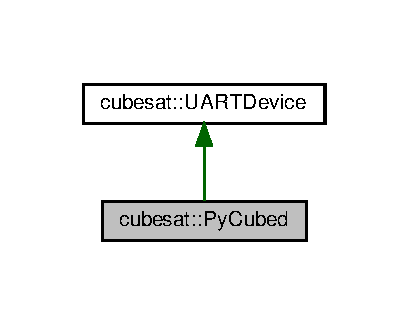
\includegraphics[width=196pt]{classcubesat_1_1PyCubed__inherit__graph}
\end{center}
\end{figure}


Collaboration diagram for cubesat\+:\+:Py\+Cubed\+:
\nopagebreak
\begin{figure}[H]
\begin{center}
\leavevmode
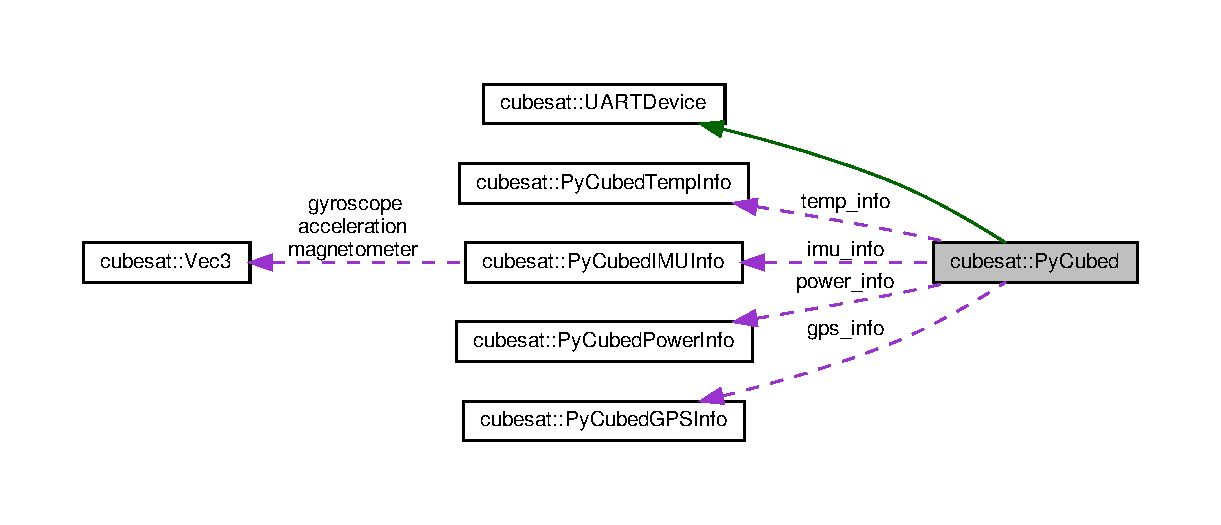
\includegraphics[width=350pt]{classcubesat_1_1PyCubed__coll__graph}
\end{center}
\end{figure}
\subsection*{Classes}
\begin{DoxyCompactItemize}
\item 
struct \hyperlink{structcubesat_1_1PyCubed_1_1MessageHandler}{Message\+Handler}
\item 
struct \hyperlink{structcubesat_1_1PyCubed_1_1MessageParser}{Message\+Parser}
\item 
struct \hyperlink{structcubesat_1_1PyCubed_1_1MessageSender}{Message\+Sender}
\end{DoxyCompactItemize}
\subsection*{Public Member Functions}
\begin{DoxyCompactItemize}
\item 
\hyperlink{classcubesat_1_1PyCubed_a30b6d7ca9cc3d8d4151eca7525c9dc61}{Py\+Cubed} (uint8\+\_\+t bus, unsigned int baud)
\begin{DoxyCompactList}\small\item\em Constructs a \hyperlink{classcubesat_1_1PyCubed}{Py\+Cubed} object using the given bus and device numbers. \end{DoxyCompactList}\item 
virtual \hyperlink{classcubesat_1_1PyCubed_ae9a69fbb6fb5df1d15984b0e11727aaa}{$\sim$\+Py\+Cubed} ()
\begin{DoxyCompactList}\small\item\em Destructor. \end{DoxyCompactList}\item 
bool \hyperlink{classcubesat_1_1PyCubed_a18980909f0eac65f0977be35336a533c}{Send\+Message} (const std\+::string \&message\+\_\+type\+\_\+str, const std\+::vector$<$ std\+::string $>$ \&args)
\begin{DoxyCompactList}\small\item\em Sends a typical (non-\/binary) message to the \hyperlink{classcubesat_1_1PyCubed}{Py\+Cubed}. \end{DoxyCompactList}\item 
void \hyperlink{classcubesat_1_1PyCubed_a1607d57f2cd19bd3b75a2c3dbbfa4955}{Add\+Message\+Handler} (const std\+::string \&message\+\_\+type\+\_\+str, \hyperlink{namespacecubesat_a3b98f17d41bf0e37fe0d382b897f9692}{Py\+Cubed\+Message\+Handler\+Callback} callback, int num\+\_\+args)
\begin{DoxyCompactList}\small\item\em Adds a message handler. \end{DoxyCompactList}\item 
void \hyperlink{classcubesat_1_1PyCubed_a7ed5f976ac8923ac539a863d89df4776}{Add\+Message\+Parser} (const std\+::string \&message\+\_\+type\+\_\+str, \hyperlink{namespacecubesat_ad7197c1bfb09998ced84827cb0dd1680}{Py\+Cubed\+Message\+Parser\+Callback} callback)
\begin{DoxyCompactList}\small\item\em Adds a message parser. \end{DoxyCompactList}\item 
bool \hyperlink{classcubesat_1_1PyCubed_afa1170644bf62745e36fcf6a479bbbee}{Startup\+Confirmation} ()
\begin{DoxyCompactList}\small\item\em Sends a message that startup was successful. \end{DoxyCompactList}\item 
bool \hyperlink{classcubesat_1_1PyCubed_a0c707ebefe9fd00e2d1e602209c1e5a6}{Handoff} ()
\begin{DoxyCompactList}\small\item\em Sends a handoff confirmation message. \end{DoxyCompactList}\item 
bool \hyperlink{classcubesat_1_1PyCubed_a1156a3504ba2c8ad1f7b6622ff9f286c}{Kill\+Radio} ()
\begin{DoxyCompactList}\small\item\em Sends a message to kill the radio. \end{DoxyCompactList}\item 
void \hyperlink{classcubesat_1_1PyCubed_acfbc0579ac92c5ef15ccf27f78bbd721}{Set\+Shutdown\+Callback} (\hyperlink{namespacecubesat_abcc8eedef699fb7e3f433200cc25e181}{Py\+Cubed\+Shutdown\+Callback} callback)
\begin{DoxyCompactList}\small\item\em Sets the callback function for when shutdown is requested. \end{DoxyCompactList}\item 
\hyperlink{structcubesat_1_1PyCubedIMUInfo}{Py\+Cubed\+I\+M\+U\+Info} \hyperlink{classcubesat_1_1PyCubed_a74fd4657765351e136367592db3e3445}{Get\+I\+M\+U\+Info} () const
\begin{DoxyCompactList}\small\item\em Returns the latest \hyperlink{classcubesat_1_1IMU}{I\+MU} information received. \end{DoxyCompactList}\item 
\hyperlink{structcubesat_1_1PyCubedGPSInfo}{Py\+Cubed\+G\+P\+S\+Info} \hyperlink{classcubesat_1_1PyCubed_a9590d2e77b63e536062209b91a393d22}{Get\+G\+P\+S\+Info} () const
\begin{DoxyCompactList}\small\item\em Returns the latest \hyperlink{classcubesat_1_1GPS}{G\+PS} information received. \end{DoxyCompactList}\item 
\hyperlink{structcubesat_1_1PyCubedTempInfo}{Py\+Cubed\+Temp\+Info} \hyperlink{classcubesat_1_1PyCubed_a1eb8a72d0782680b320a336a301927a4}{Get\+Temp\+Info} () const
\begin{DoxyCompactList}\small\item\em Returns the latest temperature information received. \end{DoxyCompactList}\item 
\hyperlink{structcubesat_1_1PyCubedPowerInfo}{Py\+Cubed\+Power\+Info} \hyperlink{classcubesat_1_1PyCubed_ae934c1fb36fbf3865ee884401dc11aaa}{Get\+Power\+Info} () const
\begin{DoxyCompactList}\small\item\em Returns the latest power information received. \end{DoxyCompactList}\item 
int \hyperlink{classcubesat_1_1PyCubed_a60887bc5d94a8f58ac1d59db50397268}{Pop\+Incoming\+Packet} (\hyperlink{structcubesat_1_1PyCubedPacket}{Py\+Cubed\+Packet} \&packet)
\begin{DoxyCompactList}\small\item\em Pops the newest radio packet from the incoming queue. \end{DoxyCompactList}\item 
int \hyperlink{classcubesat_1_1PyCubed_ab662a7193869909f84e7f61abff835d4}{Telecommand\+Outbound\+Packet} (\hyperlink{structcubesat_1_1PyCubedDataPacket}{Py\+Cubed\+Data\+Packet} packet)
\begin{DoxyCompactList}\small\item\em Sends a packet to the radio. \end{DoxyCompactList}\item 
int \hyperlink{classcubesat_1_1PyCubed_a1f9dcecafbef5dc0b285aa34c7e6a81c}{Receive\+Messages} ()
\begin{DoxyCompactList}\small\item\em Polls the \hyperlink{classcubesat_1_1PyCubed}{Py\+Cubed} device for received messages. \end{DoxyCompactList}\item 
bool \hyperlink{classcubesat_1_1PyCubed_a1a112a9d5f28f5a5cf1be27cd12d3cda}{Receive\+Next\+Message} ()
\begin{DoxyCompactList}\small\item\em Receives the next message available. \end{DoxyCompactList}\end{DoxyCompactItemize}
\subsection*{Static Private Member Functions}
\begin{DoxyCompactItemize}
\item 
static bool \hyperlink{classcubesat_1_1PyCubed_ac58a739fdf572f272776164304dc951f}{Parser\+\_\+\+P\+KT} (\hyperlink{classcubesat_1_1UARTDevice}{U\+A\+R\+T\+Device} \&uart, \hyperlink{classcubesat_1_1PyCubed}{Py\+Cubed} \&\hyperlink{pycubed__test_8cpp_ae8c4c37e7742557f28bffebe72eeef5e}{pycubed})
\begin{DoxyCompactList}\small\item\em Radio packet parser. \end{DoxyCompactList}\item 
static bool \hyperlink{classcubesat_1_1PyCubed_a1813883ff40761bffd3bdadbeac3c0ce}{Handler\+\_\+\+P\+ST} (std\+::vector$<$ std\+::string $>$ args, \hyperlink{classcubesat_1_1PyCubed}{Py\+Cubed} \&\hyperlink{pycubed__test_8cpp_ae8c4c37e7742557f28bffebe72eeef5e}{pycubed})
\begin{DoxyCompactList}\small\item\em \hyperlink{classcubesat_1_1PyCubed}{Py\+Cubed} status handler. \end{DoxyCompactList}\item 
static bool \hyperlink{classcubesat_1_1PyCubed_a4b4e36d9d30fc8c95030bdb8f6946c5e}{Handler\+\_\+\+I\+MU} (std\+::vector$<$ std\+::string $>$ args, \hyperlink{classcubesat_1_1PyCubed}{Py\+Cubed} \&\hyperlink{pycubed__test_8cpp_ae8c4c37e7742557f28bffebe72eeef5e}{pycubed})
\begin{DoxyCompactList}\small\item\em \hyperlink{classcubesat_1_1IMU}{I\+MU} handler. \end{DoxyCompactList}\item 
static bool \hyperlink{classcubesat_1_1PyCubed_a60c99d1ef8b6a6b4e5721f18348b60dd}{Handler\+\_\+\+G\+PS} (std\+::vector$<$ std\+::string $>$ args, \hyperlink{classcubesat_1_1PyCubed}{Py\+Cubed} \&\hyperlink{pycubed__test_8cpp_ae8c4c37e7742557f28bffebe72eeef5e}{pycubed})
\begin{DoxyCompactList}\small\item\em \hyperlink{classcubesat_1_1GPS}{G\+PS} handler. \end{DoxyCompactList}\item 
static bool \hyperlink{classcubesat_1_1PyCubed_a29cb9887d439e8fe784ebf9bc66187d9}{Handler\+\_\+\+T\+MP} (std\+::vector$<$ std\+::string $>$ args, \hyperlink{classcubesat_1_1PyCubed}{Py\+Cubed} \&\hyperlink{pycubed__test_8cpp_ae8c4c37e7742557f28bffebe72eeef5e}{pycubed})
\begin{DoxyCompactList}\small\item\em Temperature handler. \end{DoxyCompactList}\item 
static bool \hyperlink{classcubesat_1_1PyCubed_aeeecb0e4d2632827980174128aed304a}{Handler\+\_\+\+P\+WR} (std\+::vector$<$ std\+::string $>$ args, \hyperlink{classcubesat_1_1PyCubed}{Py\+Cubed} \&\hyperlink{pycubed__test_8cpp_ae8c4c37e7742557f28bffebe72eeef5e}{pycubed})
\begin{DoxyCompactList}\small\item\em Power handler. \end{DoxyCompactList}\end{DoxyCompactItemize}
\subsection*{Private Attributes}
\begin{DoxyCompactItemize}
\item 
\hyperlink{namespacecubesat_abcc8eedef699fb7e3f433200cc25e181}{Py\+Cubed\+Shutdown\+Callback} \hyperlink{classcubesat_1_1PyCubed_abcdb5ea9c3b544a261a3aa2ec395836f}{shutdown\+\_\+callback}
\begin{DoxyCompactList}\small\item\em The shutdown callback function. \end{DoxyCompactList}\item 
\hyperlink{namespacecubesat_a378b098737c521b2e13df70ad8ddc0ba}{Py\+Cubed\+Receive\+File\+Callback} \hyperlink{classcubesat_1_1PyCubed_a7becf9e9df5a296a53f7f4228c28451a}{receive\+\_\+file\+\_\+callback}
\begin{DoxyCompactList}\small\item\em The file receive callback. \end{DoxyCompactList}\item 
\hyperlink{structcubesat_1_1PyCubedIMUInfo}{Py\+Cubed\+I\+M\+U\+Info} \hyperlink{classcubesat_1_1PyCubed_a8ecd72592ea8f3287a520e2ac834878c}{imu\+\_\+info}
\begin{DoxyCompactList}\small\item\em Holds the last received \hyperlink{classcubesat_1_1IMU}{I\+MU} information. \end{DoxyCompactList}\item 
\hyperlink{structcubesat_1_1PyCubedGPSInfo}{Py\+Cubed\+G\+P\+S\+Info} \hyperlink{classcubesat_1_1PyCubed_a0129f71b136ecc13fc378356431ccad0}{gps\+\_\+info}
\begin{DoxyCompactList}\small\item\em Holds the last received \hyperlink{classcubesat_1_1GPS}{G\+PS} information. \end{DoxyCompactList}\item 
\hyperlink{structcubesat_1_1PyCubedTempInfo}{Py\+Cubed\+Temp\+Info} \hyperlink{classcubesat_1_1PyCubed_a5508151b5f50200754c0a10efcc0445c}{temp\+\_\+info}
\begin{DoxyCompactList}\small\item\em Holds the last received temperature information. \end{DoxyCompactList}\item 
\hyperlink{structcubesat_1_1PyCubedPowerInfo}{Py\+Cubed\+Power\+Info} \hyperlink{classcubesat_1_1PyCubed_ac1feae4409faf165aafdc38489918db3}{power\+\_\+info}
\begin{DoxyCompactList}\small\item\em Holds the last received power information. \end{DoxyCompactList}\item 
std\+::queue$<$ \hyperlink{structcubesat_1_1PyCubedPacket}{Py\+Cubed\+Packet} $>$ \hyperlink{classcubesat_1_1PyCubed_a909673179f44b10128f01bd579bc13ba}{incoming\+\_\+packets}
\begin{DoxyCompactList}\small\item\em Holds the incoming radio packets. \end{DoxyCompactList}\item 
std\+::unordered\+\_\+map$<$ std\+::string, \hyperlink{structcubesat_1_1PyCubed_1_1MessageParser}{Message\+Parser} $>$ \hyperlink{classcubesat_1_1PyCubed_a284d1cfcdd19675e2b96913018192928}{parsers}
\begin{DoxyCompactList}\small\item\em The added message parsers. \end{DoxyCompactList}\item 
std\+::unordered\+\_\+map$<$ std\+::string, \hyperlink{structcubesat_1_1PyCubed_1_1MessageHandler}{Message\+Handler} $>$ \hyperlink{classcubesat_1_1PyCubed_aacc466db4b35e383eedd385db64522a1}{handlers}
\begin{DoxyCompactList}\small\item\em The added message handlers. \end{DoxyCompactList}\end{DoxyCompactItemize}
\subsection*{Additional Inherited Members}


\subsection{Detailed Description}
Provides access to the \hyperlink{classcubesat_1_1PyCubed}{Py\+Cubed} mainboard. 

\subsection{Constructor \& Destructor Documentation}
\mbox{\Hypertarget{classcubesat_1_1PyCubed_a30b6d7ca9cc3d8d4151eca7525c9dc61}\label{classcubesat_1_1PyCubed_a30b6d7ca9cc3d8d4151eca7525c9dc61}} 
\index{cubesat\+::\+Py\+Cubed@{cubesat\+::\+Py\+Cubed}!Py\+Cubed@{Py\+Cubed}}
\index{Py\+Cubed@{Py\+Cubed}!cubesat\+::\+Py\+Cubed@{cubesat\+::\+Py\+Cubed}}
\subsubsection{\texorpdfstring{Py\+Cubed()}{PyCubed()}}
{\footnotesize\ttfamily Py\+Cubed\+::\+Py\+Cubed (\begin{DoxyParamCaption}\item[{uint8\+\_\+t}]{bus,  }\item[{unsigned int}]{baud }\end{DoxyParamCaption})}



Constructs a \hyperlink{classcubesat_1_1PyCubed}{Py\+Cubed} object using the given bus and device numbers. 


\begin{DoxyParams}{Parameters}
{\em bus} & The U\+A\+RT bus number to use \\
\hline
{\em device} & The device number to use \\
\hline
\end{DoxyParams}
\mbox{\Hypertarget{classcubesat_1_1PyCubed_ae9a69fbb6fb5df1d15984b0e11727aaa}\label{classcubesat_1_1PyCubed_ae9a69fbb6fb5df1d15984b0e11727aaa}} 
\index{cubesat\+::\+Py\+Cubed@{cubesat\+::\+Py\+Cubed}!````~Py\+Cubed@{$\sim$\+Py\+Cubed}}
\index{````~Py\+Cubed@{$\sim$\+Py\+Cubed}!cubesat\+::\+Py\+Cubed@{cubesat\+::\+Py\+Cubed}}
\subsubsection{\texorpdfstring{$\sim$\+Py\+Cubed()}{~PyCubed()}}
{\footnotesize\ttfamily Py\+Cubed\+::$\sim$\+Py\+Cubed (\begin{DoxyParamCaption}{ }\end{DoxyParamCaption})\hspace{0.3cm}{\ttfamily [virtual]}}



Destructor. 



\subsection{Member Function Documentation}
\mbox{\Hypertarget{classcubesat_1_1PyCubed_a1607d57f2cd19bd3b75a2c3dbbfa4955}\label{classcubesat_1_1PyCubed_a1607d57f2cd19bd3b75a2c3dbbfa4955}} 
\index{cubesat\+::\+Py\+Cubed@{cubesat\+::\+Py\+Cubed}!Add\+Message\+Handler@{Add\+Message\+Handler}}
\index{Add\+Message\+Handler@{Add\+Message\+Handler}!cubesat\+::\+Py\+Cubed@{cubesat\+::\+Py\+Cubed}}
\subsubsection{\texorpdfstring{Add\+Message\+Handler()}{AddMessageHandler()}}
{\footnotesize\ttfamily void cubesat\+::\+Py\+Cubed\+::\+Add\+Message\+Handler (\begin{DoxyParamCaption}\item[{const std\+::string \&}]{message\+\_\+type\+\_\+str,  }\item[{\hyperlink{namespacecubesat_a3b98f17d41bf0e37fe0d382b897f9692}{Py\+Cubed\+Message\+Handler\+Callback}}]{callback,  }\item[{int}]{num\+\_\+args }\end{DoxyParamCaption})\hspace{0.3cm}{\ttfamily [inline]}}



Adds a message handler. 


\begin{DoxyParams}{Parameters}
{\em message\+\_\+type\+\_\+str} & The message type string to add support for \\
\hline
{\em callback} & The function to call when this message type is received \\
\hline
{\em num\+\_\+args} & The number of arguments expected \\
\hline
\end{DoxyParams}
\mbox{\Hypertarget{classcubesat_1_1PyCubed_a7ed5f976ac8923ac539a863d89df4776}\label{classcubesat_1_1PyCubed_a7ed5f976ac8923ac539a863d89df4776}} 
\index{cubesat\+::\+Py\+Cubed@{cubesat\+::\+Py\+Cubed}!Add\+Message\+Parser@{Add\+Message\+Parser}}
\index{Add\+Message\+Parser@{Add\+Message\+Parser}!cubesat\+::\+Py\+Cubed@{cubesat\+::\+Py\+Cubed}}
\subsubsection{\texorpdfstring{Add\+Message\+Parser()}{AddMessageParser()}}
{\footnotesize\ttfamily void cubesat\+::\+Py\+Cubed\+::\+Add\+Message\+Parser (\begin{DoxyParamCaption}\item[{const std\+::string \&}]{message\+\_\+type\+\_\+str,  }\item[{\hyperlink{namespacecubesat_ad7197c1bfb09998ced84827cb0dd1680}{Py\+Cubed\+Message\+Parser\+Callback}}]{callback }\end{DoxyParamCaption})\hspace{0.3cm}{\ttfamily [inline]}}



Adds a message parser. 


\begin{DoxyParams}{Parameters}
{\em message\+\_\+type\+\_\+str} & The message type string to add support for \\
\hline
{\em callback} & The function to call when this message type is received \\
\hline
\end{DoxyParams}
\mbox{\Hypertarget{classcubesat_1_1PyCubed_a9590d2e77b63e536062209b91a393d22}\label{classcubesat_1_1PyCubed_a9590d2e77b63e536062209b91a393d22}} 
\index{cubesat\+::\+Py\+Cubed@{cubesat\+::\+Py\+Cubed}!Get\+G\+P\+S\+Info@{Get\+G\+P\+S\+Info}}
\index{Get\+G\+P\+S\+Info@{Get\+G\+P\+S\+Info}!cubesat\+::\+Py\+Cubed@{cubesat\+::\+Py\+Cubed}}
\subsubsection{\texorpdfstring{Get\+G\+P\+S\+Info()}{GetGPSInfo()}}
{\footnotesize\ttfamily \hyperlink{structcubesat_1_1PyCubedGPSInfo}{Py\+Cubed\+G\+P\+S\+Info} cubesat\+::\+Py\+Cubed\+::\+Get\+G\+P\+S\+Info (\begin{DoxyParamCaption}{ }\end{DoxyParamCaption}) const\hspace{0.3cm}{\ttfamily [inline]}}



Returns the latest \hyperlink{classcubesat_1_1GPS}{G\+PS} information received. 

\begin{DoxyReturn}{Returns}
The \hyperlink{classcubesat_1_1GPS}{G\+PS} information 
\end{DoxyReturn}
\mbox{\Hypertarget{classcubesat_1_1PyCubed_a74fd4657765351e136367592db3e3445}\label{classcubesat_1_1PyCubed_a74fd4657765351e136367592db3e3445}} 
\index{cubesat\+::\+Py\+Cubed@{cubesat\+::\+Py\+Cubed}!Get\+I\+M\+U\+Info@{Get\+I\+M\+U\+Info}}
\index{Get\+I\+M\+U\+Info@{Get\+I\+M\+U\+Info}!cubesat\+::\+Py\+Cubed@{cubesat\+::\+Py\+Cubed}}
\subsubsection{\texorpdfstring{Get\+I\+M\+U\+Info()}{GetIMUInfo()}}
{\footnotesize\ttfamily \hyperlink{structcubesat_1_1PyCubedIMUInfo}{Py\+Cubed\+I\+M\+U\+Info} cubesat\+::\+Py\+Cubed\+::\+Get\+I\+M\+U\+Info (\begin{DoxyParamCaption}{ }\end{DoxyParamCaption}) const\hspace{0.3cm}{\ttfamily [inline]}}



Returns the latest \hyperlink{classcubesat_1_1IMU}{I\+MU} information received. 

\begin{DoxyReturn}{Returns}
The \hyperlink{classcubesat_1_1IMU}{I\+MU} information 
\end{DoxyReturn}
\mbox{\Hypertarget{classcubesat_1_1PyCubed_ae934c1fb36fbf3865ee884401dc11aaa}\label{classcubesat_1_1PyCubed_ae934c1fb36fbf3865ee884401dc11aaa}} 
\index{cubesat\+::\+Py\+Cubed@{cubesat\+::\+Py\+Cubed}!Get\+Power\+Info@{Get\+Power\+Info}}
\index{Get\+Power\+Info@{Get\+Power\+Info}!cubesat\+::\+Py\+Cubed@{cubesat\+::\+Py\+Cubed}}
\subsubsection{\texorpdfstring{Get\+Power\+Info()}{GetPowerInfo()}}
{\footnotesize\ttfamily \hyperlink{structcubesat_1_1PyCubedPowerInfo}{Py\+Cubed\+Power\+Info} cubesat\+::\+Py\+Cubed\+::\+Get\+Power\+Info (\begin{DoxyParamCaption}{ }\end{DoxyParamCaption}) const\hspace{0.3cm}{\ttfamily [inline]}}



Returns the latest power information received. 

\begin{DoxyReturn}{Returns}
The power information 
\end{DoxyReturn}
\mbox{\Hypertarget{classcubesat_1_1PyCubed_a1eb8a72d0782680b320a336a301927a4}\label{classcubesat_1_1PyCubed_a1eb8a72d0782680b320a336a301927a4}} 
\index{cubesat\+::\+Py\+Cubed@{cubesat\+::\+Py\+Cubed}!Get\+Temp\+Info@{Get\+Temp\+Info}}
\index{Get\+Temp\+Info@{Get\+Temp\+Info}!cubesat\+::\+Py\+Cubed@{cubesat\+::\+Py\+Cubed}}
\subsubsection{\texorpdfstring{Get\+Temp\+Info()}{GetTempInfo()}}
{\footnotesize\ttfamily \hyperlink{structcubesat_1_1PyCubedTempInfo}{Py\+Cubed\+Temp\+Info} cubesat\+::\+Py\+Cubed\+::\+Get\+Temp\+Info (\begin{DoxyParamCaption}{ }\end{DoxyParamCaption}) const\hspace{0.3cm}{\ttfamily [inline]}}



Returns the latest temperature information received. 

\begin{DoxyReturn}{Returns}
The temperature information 
\end{DoxyReturn}
\mbox{\Hypertarget{classcubesat_1_1PyCubed_a60c99d1ef8b6a6b4e5721f18348b60dd}\label{classcubesat_1_1PyCubed_a60c99d1ef8b6a6b4e5721f18348b60dd}} 
\index{cubesat\+::\+Py\+Cubed@{cubesat\+::\+Py\+Cubed}!Handler\+\_\+\+G\+PS@{Handler\+\_\+\+G\+PS}}
\index{Handler\+\_\+\+G\+PS@{Handler\+\_\+\+G\+PS}!cubesat\+::\+Py\+Cubed@{cubesat\+::\+Py\+Cubed}}
\subsubsection{\texorpdfstring{Handler\+\_\+\+G\+P\+S()}{Handler\_GPS()}}
{\footnotesize\ttfamily bool Py\+Cubed\+::\+Handler\+\_\+\+G\+PS (\begin{DoxyParamCaption}\item[{std\+::vector$<$ std\+::string $>$}]{args,  }\item[{\hyperlink{classcubesat_1_1PyCubed}{Py\+Cubed} \&}]{pycubed }\end{DoxyParamCaption})\hspace{0.3cm}{\ttfamily [static]}, {\ttfamily [private]}}



\hyperlink{classcubesat_1_1GPS}{G\+PS} handler. 

\mbox{\Hypertarget{classcubesat_1_1PyCubed_a4b4e36d9d30fc8c95030bdb8f6946c5e}\label{classcubesat_1_1PyCubed_a4b4e36d9d30fc8c95030bdb8f6946c5e}} 
\index{cubesat\+::\+Py\+Cubed@{cubesat\+::\+Py\+Cubed}!Handler\+\_\+\+I\+MU@{Handler\+\_\+\+I\+MU}}
\index{Handler\+\_\+\+I\+MU@{Handler\+\_\+\+I\+MU}!cubesat\+::\+Py\+Cubed@{cubesat\+::\+Py\+Cubed}}
\subsubsection{\texorpdfstring{Handler\+\_\+\+I\+M\+U()}{Handler\_IMU()}}
{\footnotesize\ttfamily bool Py\+Cubed\+::\+Handler\+\_\+\+I\+MU (\begin{DoxyParamCaption}\item[{std\+::vector$<$ std\+::string $>$}]{args,  }\item[{\hyperlink{classcubesat_1_1PyCubed}{Py\+Cubed} \&}]{pycubed }\end{DoxyParamCaption})\hspace{0.3cm}{\ttfamily [static]}, {\ttfamily [private]}}



\hyperlink{classcubesat_1_1IMU}{I\+MU} handler. 

\mbox{\Hypertarget{classcubesat_1_1PyCubed_a1813883ff40761bffd3bdadbeac3c0ce}\label{classcubesat_1_1PyCubed_a1813883ff40761bffd3bdadbeac3c0ce}} 
\index{cubesat\+::\+Py\+Cubed@{cubesat\+::\+Py\+Cubed}!Handler\+\_\+\+P\+ST@{Handler\+\_\+\+P\+ST}}
\index{Handler\+\_\+\+P\+ST@{Handler\+\_\+\+P\+ST}!cubesat\+::\+Py\+Cubed@{cubesat\+::\+Py\+Cubed}}
\subsubsection{\texorpdfstring{Handler\+\_\+\+P\+S\+T()}{Handler\_PST()}}
{\footnotesize\ttfamily bool Py\+Cubed\+::\+Handler\+\_\+\+P\+ST (\begin{DoxyParamCaption}\item[{std\+::vector$<$ std\+::string $>$}]{args,  }\item[{\hyperlink{classcubesat_1_1PyCubed}{Py\+Cubed} \&}]{pycubed }\end{DoxyParamCaption})\hspace{0.3cm}{\ttfamily [static]}, {\ttfamily [private]}}



\hyperlink{classcubesat_1_1PyCubed}{Py\+Cubed} status handler. 

\mbox{\Hypertarget{classcubesat_1_1PyCubed_aeeecb0e4d2632827980174128aed304a}\label{classcubesat_1_1PyCubed_aeeecb0e4d2632827980174128aed304a}} 
\index{cubesat\+::\+Py\+Cubed@{cubesat\+::\+Py\+Cubed}!Handler\+\_\+\+P\+WR@{Handler\+\_\+\+P\+WR}}
\index{Handler\+\_\+\+P\+WR@{Handler\+\_\+\+P\+WR}!cubesat\+::\+Py\+Cubed@{cubesat\+::\+Py\+Cubed}}
\subsubsection{\texorpdfstring{Handler\+\_\+\+P\+W\+R()}{Handler\_PWR()}}
{\footnotesize\ttfamily bool Py\+Cubed\+::\+Handler\+\_\+\+P\+WR (\begin{DoxyParamCaption}\item[{std\+::vector$<$ std\+::string $>$}]{args,  }\item[{\hyperlink{classcubesat_1_1PyCubed}{Py\+Cubed} \&}]{pycubed }\end{DoxyParamCaption})\hspace{0.3cm}{\ttfamily [static]}, {\ttfamily [private]}}



Power handler. 

\mbox{\Hypertarget{classcubesat_1_1PyCubed_a29cb9887d439e8fe784ebf9bc66187d9}\label{classcubesat_1_1PyCubed_a29cb9887d439e8fe784ebf9bc66187d9}} 
\index{cubesat\+::\+Py\+Cubed@{cubesat\+::\+Py\+Cubed}!Handler\+\_\+\+T\+MP@{Handler\+\_\+\+T\+MP}}
\index{Handler\+\_\+\+T\+MP@{Handler\+\_\+\+T\+MP}!cubesat\+::\+Py\+Cubed@{cubesat\+::\+Py\+Cubed}}
\subsubsection{\texorpdfstring{Handler\+\_\+\+T\+M\+P()}{Handler\_TMP()}}
{\footnotesize\ttfamily bool Py\+Cubed\+::\+Handler\+\_\+\+T\+MP (\begin{DoxyParamCaption}\item[{std\+::vector$<$ std\+::string $>$}]{args,  }\item[{\hyperlink{classcubesat_1_1PyCubed}{Py\+Cubed} \&}]{pycubed }\end{DoxyParamCaption})\hspace{0.3cm}{\ttfamily [static]}, {\ttfamily [private]}}



Temperature handler. 

\mbox{\Hypertarget{classcubesat_1_1PyCubed_a0c707ebefe9fd00e2d1e602209c1e5a6}\label{classcubesat_1_1PyCubed_a0c707ebefe9fd00e2d1e602209c1e5a6}} 
\index{cubesat\+::\+Py\+Cubed@{cubesat\+::\+Py\+Cubed}!Handoff@{Handoff}}
\index{Handoff@{Handoff}!cubesat\+::\+Py\+Cubed@{cubesat\+::\+Py\+Cubed}}
\subsubsection{\texorpdfstring{Handoff()}{Handoff()}}
{\footnotesize\ttfamily bool cubesat\+::\+Py\+Cubed\+::\+Handoff (\begin{DoxyParamCaption}{ }\end{DoxyParamCaption})\hspace{0.3cm}{\ttfamily [inline]}}



Sends a handoff confirmation message. 

\begin{DoxyReturn}{Returns}
The status of the operation 
\end{DoxyReturn}
\mbox{\Hypertarget{classcubesat_1_1PyCubed_a1156a3504ba2c8ad1f7b6622ff9f286c}\label{classcubesat_1_1PyCubed_a1156a3504ba2c8ad1f7b6622ff9f286c}} 
\index{cubesat\+::\+Py\+Cubed@{cubesat\+::\+Py\+Cubed}!Kill\+Radio@{Kill\+Radio}}
\index{Kill\+Radio@{Kill\+Radio}!cubesat\+::\+Py\+Cubed@{cubesat\+::\+Py\+Cubed}}
\subsubsection{\texorpdfstring{Kill\+Radio()}{KillRadio()}}
{\footnotesize\ttfamily bool cubesat\+::\+Py\+Cubed\+::\+Kill\+Radio (\begin{DoxyParamCaption}{ }\end{DoxyParamCaption})\hspace{0.3cm}{\ttfamily [inline]}}



Sends a message to kill the radio. 

\begin{DoxyReturn}{Returns}
The status of the operation 
\end{DoxyReturn}
\mbox{\Hypertarget{classcubesat_1_1PyCubed_ac58a739fdf572f272776164304dc951f}\label{classcubesat_1_1PyCubed_ac58a739fdf572f272776164304dc951f}} 
\index{cubesat\+::\+Py\+Cubed@{cubesat\+::\+Py\+Cubed}!Parser\+\_\+\+P\+KT@{Parser\+\_\+\+P\+KT}}
\index{Parser\+\_\+\+P\+KT@{Parser\+\_\+\+P\+KT}!cubesat\+::\+Py\+Cubed@{cubesat\+::\+Py\+Cubed}}
\subsubsection{\texorpdfstring{Parser\+\_\+\+P\+K\+T()}{Parser\_PKT()}}
{\footnotesize\ttfamily bool Py\+Cubed\+::\+Parser\+\_\+\+P\+KT (\begin{DoxyParamCaption}\item[{\hyperlink{classcubesat_1_1UARTDevice}{U\+A\+R\+T\+Device} \&}]{uart,  }\item[{\hyperlink{classcubesat_1_1PyCubed}{Py\+Cubed} \&}]{pycubed }\end{DoxyParamCaption})\hspace{0.3cm}{\ttfamily [static]}, {\ttfamily [private]}}



Radio packet parser. 

\mbox{\Hypertarget{classcubesat_1_1PyCubed_a60887bc5d94a8f58ac1d59db50397268}\label{classcubesat_1_1PyCubed_a60887bc5d94a8f58ac1d59db50397268}} 
\index{cubesat\+::\+Py\+Cubed@{cubesat\+::\+Py\+Cubed}!Pop\+Incoming\+Packet@{Pop\+Incoming\+Packet}}
\index{Pop\+Incoming\+Packet@{Pop\+Incoming\+Packet}!cubesat\+::\+Py\+Cubed@{cubesat\+::\+Py\+Cubed}}
\subsubsection{\texorpdfstring{Pop\+Incoming\+Packet()}{PopIncomingPacket()}}
{\footnotesize\ttfamily int Py\+Cubed\+::\+Pop\+Incoming\+Packet (\begin{DoxyParamCaption}\item[{\hyperlink{structcubesat_1_1PyCubedPacket}{Py\+Cubed\+Packet} \&}]{packet }\end{DoxyParamCaption})}



Pops the newest radio packet from the incoming queue. 


\begin{DoxyParams}{Parameters}
{\em packet} & The output variable for the packet \\
\hline
\end{DoxyParams}
\begin{DoxyReturn}{Returns}
The packet size 
\end{DoxyReturn}
\mbox{\Hypertarget{classcubesat_1_1PyCubed_a1f9dcecafbef5dc0b285aa34c7e6a81c}\label{classcubesat_1_1PyCubed_a1f9dcecafbef5dc0b285aa34c7e6a81c}} 
\index{cubesat\+::\+Py\+Cubed@{cubesat\+::\+Py\+Cubed}!Receive\+Messages@{Receive\+Messages}}
\index{Receive\+Messages@{Receive\+Messages}!cubesat\+::\+Py\+Cubed@{cubesat\+::\+Py\+Cubed}}
\subsubsection{\texorpdfstring{Receive\+Messages()}{ReceiveMessages()}}
{\footnotesize\ttfamily int Py\+Cubed\+::\+Receive\+Messages (\begin{DoxyParamCaption}{ }\end{DoxyParamCaption})}



Polls the \hyperlink{classcubesat_1_1PyCubed}{Py\+Cubed} device for received messages. 

\begin{DoxyReturn}{Returns}
The number of messages received 
\end{DoxyReturn}
\mbox{\Hypertarget{classcubesat_1_1PyCubed_a1a112a9d5f28f5a5cf1be27cd12d3cda}\label{classcubesat_1_1PyCubed_a1a112a9d5f28f5a5cf1be27cd12d3cda}} 
\index{cubesat\+::\+Py\+Cubed@{cubesat\+::\+Py\+Cubed}!Receive\+Next\+Message@{Receive\+Next\+Message}}
\index{Receive\+Next\+Message@{Receive\+Next\+Message}!cubesat\+::\+Py\+Cubed@{cubesat\+::\+Py\+Cubed}}
\subsubsection{\texorpdfstring{Receive\+Next\+Message()}{ReceiveNextMessage()}}
{\footnotesize\ttfamily bool Py\+Cubed\+::\+Receive\+Next\+Message (\begin{DoxyParamCaption}{ }\end{DoxyParamCaption})}



Receives the next message available. 

\begin{DoxyReturn}{Returns}
True if the message was read successfully 
\end{DoxyReturn}
\mbox{\Hypertarget{classcubesat_1_1PyCubed_a18980909f0eac65f0977be35336a533c}\label{classcubesat_1_1PyCubed_a18980909f0eac65f0977be35336a533c}} 
\index{cubesat\+::\+Py\+Cubed@{cubesat\+::\+Py\+Cubed}!Send\+Message@{Send\+Message}}
\index{Send\+Message@{Send\+Message}!cubesat\+::\+Py\+Cubed@{cubesat\+::\+Py\+Cubed}}
\subsubsection{\texorpdfstring{Send\+Message()}{SendMessage()}}
{\footnotesize\ttfamily bool Py\+Cubed\+::\+Send\+Message (\begin{DoxyParamCaption}\item[{const std\+::string \&}]{message\+\_\+type\+\_\+str,  }\item[{const std\+::vector$<$ std\+::string $>$ \&}]{args }\end{DoxyParamCaption})}



Sends a typical (non-\/binary) message to the \hyperlink{classcubesat_1_1PyCubed}{Py\+Cubed}. 


\begin{DoxyParams}{Parameters}
{\em message\+\_\+type\+\_\+str} & The message type string \\
\hline
{\em args} & The string arguments to write \\
\hline
\end{DoxyParams}
\begin{DoxyReturn}{Returns}
True upon success 
\end{DoxyReturn}
\mbox{\Hypertarget{classcubesat_1_1PyCubed_acfbc0579ac92c5ef15ccf27f78bbd721}\label{classcubesat_1_1PyCubed_acfbc0579ac92c5ef15ccf27f78bbd721}} 
\index{cubesat\+::\+Py\+Cubed@{cubesat\+::\+Py\+Cubed}!Set\+Shutdown\+Callback@{Set\+Shutdown\+Callback}}
\index{Set\+Shutdown\+Callback@{Set\+Shutdown\+Callback}!cubesat\+::\+Py\+Cubed@{cubesat\+::\+Py\+Cubed}}
\subsubsection{\texorpdfstring{Set\+Shutdown\+Callback()}{SetShutdownCallback()}}
{\footnotesize\ttfamily void cubesat\+::\+Py\+Cubed\+::\+Set\+Shutdown\+Callback (\begin{DoxyParamCaption}\item[{\hyperlink{namespacecubesat_abcc8eedef699fb7e3f433200cc25e181}{Py\+Cubed\+Shutdown\+Callback}}]{callback }\end{DoxyParamCaption})\hspace{0.3cm}{\ttfamily [inline]}}



Sets the callback function for when shutdown is requested. 


\begin{DoxyParams}{Parameters}
{\em callback} & The function to call \\
\hline
\end{DoxyParams}
\mbox{\Hypertarget{classcubesat_1_1PyCubed_afa1170644bf62745e36fcf6a479bbbee}\label{classcubesat_1_1PyCubed_afa1170644bf62745e36fcf6a479bbbee}} 
\index{cubesat\+::\+Py\+Cubed@{cubesat\+::\+Py\+Cubed}!Startup\+Confirmation@{Startup\+Confirmation}}
\index{Startup\+Confirmation@{Startup\+Confirmation}!cubesat\+::\+Py\+Cubed@{cubesat\+::\+Py\+Cubed}}
\subsubsection{\texorpdfstring{Startup\+Confirmation()}{StartupConfirmation()}}
{\footnotesize\ttfamily bool cubesat\+::\+Py\+Cubed\+::\+Startup\+Confirmation (\begin{DoxyParamCaption}{ }\end{DoxyParamCaption})\hspace{0.3cm}{\ttfamily [inline]}}



Sends a message that startup was successful. 

\begin{DoxyReturn}{Returns}
The status of the operation 
\end{DoxyReturn}
\mbox{\Hypertarget{classcubesat_1_1PyCubed_ab662a7193869909f84e7f61abff835d4}\label{classcubesat_1_1PyCubed_ab662a7193869909f84e7f61abff835d4}} 
\index{cubesat\+::\+Py\+Cubed@{cubesat\+::\+Py\+Cubed}!Telecommand\+Outbound\+Packet@{Telecommand\+Outbound\+Packet}}
\index{Telecommand\+Outbound\+Packet@{Telecommand\+Outbound\+Packet}!cubesat\+::\+Py\+Cubed@{cubesat\+::\+Py\+Cubed}}
\subsubsection{\texorpdfstring{Telecommand\+Outbound\+Packet()}{TelecommandOutboundPacket()}}
{\footnotesize\ttfamily int Py\+Cubed\+::\+Telecommand\+Outbound\+Packet (\begin{DoxyParamCaption}\item[{\hyperlink{structcubesat_1_1PyCubedDataPacket}{Py\+Cubed\+Data\+Packet}}]{packet }\end{DoxyParamCaption})}



Sends a packet to the radio. 


\begin{DoxyParams}{Parameters}
{\em packet} & The packet \\
\hline
\end{DoxyParams}
\begin{DoxyReturn}{Returns}
The number of bytes written 
\end{DoxyReturn}


\subsection{Member Data Documentation}
\mbox{\Hypertarget{classcubesat_1_1PyCubed_a0129f71b136ecc13fc378356431ccad0}\label{classcubesat_1_1PyCubed_a0129f71b136ecc13fc378356431ccad0}} 
\index{cubesat\+::\+Py\+Cubed@{cubesat\+::\+Py\+Cubed}!gps\+\_\+info@{gps\+\_\+info}}
\index{gps\+\_\+info@{gps\+\_\+info}!cubesat\+::\+Py\+Cubed@{cubesat\+::\+Py\+Cubed}}
\subsubsection{\texorpdfstring{gps\+\_\+info}{gps\_info}}
{\footnotesize\ttfamily \hyperlink{structcubesat_1_1PyCubedGPSInfo}{Py\+Cubed\+G\+P\+S\+Info} cubesat\+::\+Py\+Cubed\+::gps\+\_\+info\hspace{0.3cm}{\ttfamily [private]}}



Holds the last received \hyperlink{classcubesat_1_1GPS}{G\+PS} information. 

\mbox{\Hypertarget{classcubesat_1_1PyCubed_aacc466db4b35e383eedd385db64522a1}\label{classcubesat_1_1PyCubed_aacc466db4b35e383eedd385db64522a1}} 
\index{cubesat\+::\+Py\+Cubed@{cubesat\+::\+Py\+Cubed}!handlers@{handlers}}
\index{handlers@{handlers}!cubesat\+::\+Py\+Cubed@{cubesat\+::\+Py\+Cubed}}
\subsubsection{\texorpdfstring{handlers}{handlers}}
{\footnotesize\ttfamily std\+::unordered\+\_\+map$<$std\+::string, \hyperlink{structcubesat_1_1PyCubed_1_1MessageHandler}{Message\+Handler}$>$ cubesat\+::\+Py\+Cubed\+::handlers\hspace{0.3cm}{\ttfamily [private]}}



The added message handlers. 

\mbox{\Hypertarget{classcubesat_1_1PyCubed_a8ecd72592ea8f3287a520e2ac834878c}\label{classcubesat_1_1PyCubed_a8ecd72592ea8f3287a520e2ac834878c}} 
\index{cubesat\+::\+Py\+Cubed@{cubesat\+::\+Py\+Cubed}!imu\+\_\+info@{imu\+\_\+info}}
\index{imu\+\_\+info@{imu\+\_\+info}!cubesat\+::\+Py\+Cubed@{cubesat\+::\+Py\+Cubed}}
\subsubsection{\texorpdfstring{imu\+\_\+info}{imu\_info}}
{\footnotesize\ttfamily \hyperlink{structcubesat_1_1PyCubedIMUInfo}{Py\+Cubed\+I\+M\+U\+Info} cubesat\+::\+Py\+Cubed\+::imu\+\_\+info\hspace{0.3cm}{\ttfamily [private]}}



Holds the last received \hyperlink{classcubesat_1_1IMU}{I\+MU} information. 

\mbox{\Hypertarget{classcubesat_1_1PyCubed_a909673179f44b10128f01bd579bc13ba}\label{classcubesat_1_1PyCubed_a909673179f44b10128f01bd579bc13ba}} 
\index{cubesat\+::\+Py\+Cubed@{cubesat\+::\+Py\+Cubed}!incoming\+\_\+packets@{incoming\+\_\+packets}}
\index{incoming\+\_\+packets@{incoming\+\_\+packets}!cubesat\+::\+Py\+Cubed@{cubesat\+::\+Py\+Cubed}}
\subsubsection{\texorpdfstring{incoming\+\_\+packets}{incoming\_packets}}
{\footnotesize\ttfamily std\+::queue$<$\hyperlink{structcubesat_1_1PyCubedPacket}{Py\+Cubed\+Packet}$>$ cubesat\+::\+Py\+Cubed\+::incoming\+\_\+packets\hspace{0.3cm}{\ttfamily [private]}}



Holds the incoming radio packets. 

\mbox{\Hypertarget{classcubesat_1_1PyCubed_a284d1cfcdd19675e2b96913018192928}\label{classcubesat_1_1PyCubed_a284d1cfcdd19675e2b96913018192928}} 
\index{cubesat\+::\+Py\+Cubed@{cubesat\+::\+Py\+Cubed}!parsers@{parsers}}
\index{parsers@{parsers}!cubesat\+::\+Py\+Cubed@{cubesat\+::\+Py\+Cubed}}
\subsubsection{\texorpdfstring{parsers}{parsers}}
{\footnotesize\ttfamily std\+::unordered\+\_\+map$<$std\+::string, \hyperlink{structcubesat_1_1PyCubed_1_1MessageParser}{Message\+Parser}$>$ cubesat\+::\+Py\+Cubed\+::parsers\hspace{0.3cm}{\ttfamily [private]}}



The added message parsers. 

\mbox{\Hypertarget{classcubesat_1_1PyCubed_ac1feae4409faf165aafdc38489918db3}\label{classcubesat_1_1PyCubed_ac1feae4409faf165aafdc38489918db3}} 
\index{cubesat\+::\+Py\+Cubed@{cubesat\+::\+Py\+Cubed}!power\+\_\+info@{power\+\_\+info}}
\index{power\+\_\+info@{power\+\_\+info}!cubesat\+::\+Py\+Cubed@{cubesat\+::\+Py\+Cubed}}
\subsubsection{\texorpdfstring{power\+\_\+info}{power\_info}}
{\footnotesize\ttfamily \hyperlink{structcubesat_1_1PyCubedPowerInfo}{Py\+Cubed\+Power\+Info} cubesat\+::\+Py\+Cubed\+::power\+\_\+info\hspace{0.3cm}{\ttfamily [private]}}



Holds the last received power information. 

\mbox{\Hypertarget{classcubesat_1_1PyCubed_a7becf9e9df5a296a53f7f4228c28451a}\label{classcubesat_1_1PyCubed_a7becf9e9df5a296a53f7f4228c28451a}} 
\index{cubesat\+::\+Py\+Cubed@{cubesat\+::\+Py\+Cubed}!receive\+\_\+file\+\_\+callback@{receive\+\_\+file\+\_\+callback}}
\index{receive\+\_\+file\+\_\+callback@{receive\+\_\+file\+\_\+callback}!cubesat\+::\+Py\+Cubed@{cubesat\+::\+Py\+Cubed}}
\subsubsection{\texorpdfstring{receive\+\_\+file\+\_\+callback}{receive\_file\_callback}}
{\footnotesize\ttfamily \hyperlink{namespacecubesat_a378b098737c521b2e13df70ad8ddc0ba}{Py\+Cubed\+Receive\+File\+Callback} cubesat\+::\+Py\+Cubed\+::receive\+\_\+file\+\_\+callback\hspace{0.3cm}{\ttfamily [private]}}



The file receive callback. 

\mbox{\Hypertarget{classcubesat_1_1PyCubed_abcdb5ea9c3b544a261a3aa2ec395836f}\label{classcubesat_1_1PyCubed_abcdb5ea9c3b544a261a3aa2ec395836f}} 
\index{cubesat\+::\+Py\+Cubed@{cubesat\+::\+Py\+Cubed}!shutdown\+\_\+callback@{shutdown\+\_\+callback}}
\index{shutdown\+\_\+callback@{shutdown\+\_\+callback}!cubesat\+::\+Py\+Cubed@{cubesat\+::\+Py\+Cubed}}
\subsubsection{\texorpdfstring{shutdown\+\_\+callback}{shutdown\_callback}}
{\footnotesize\ttfamily \hyperlink{namespacecubesat_abcc8eedef699fb7e3f433200cc25e181}{Py\+Cubed\+Shutdown\+Callback} cubesat\+::\+Py\+Cubed\+::shutdown\+\_\+callback\hspace{0.3cm}{\ttfamily [private]}}



The shutdown callback function. 

\mbox{\Hypertarget{classcubesat_1_1PyCubed_a5508151b5f50200754c0a10efcc0445c}\label{classcubesat_1_1PyCubed_a5508151b5f50200754c0a10efcc0445c}} 
\index{cubesat\+::\+Py\+Cubed@{cubesat\+::\+Py\+Cubed}!temp\+\_\+info@{temp\+\_\+info}}
\index{temp\+\_\+info@{temp\+\_\+info}!cubesat\+::\+Py\+Cubed@{cubesat\+::\+Py\+Cubed}}
\subsubsection{\texorpdfstring{temp\+\_\+info}{temp\_info}}
{\footnotesize\ttfamily \hyperlink{structcubesat_1_1PyCubedTempInfo}{Py\+Cubed\+Temp\+Info} cubesat\+::\+Py\+Cubed\+::temp\+\_\+info\hspace{0.3cm}{\ttfamily [private]}}



Holds the last received temperature information. 



The documentation for this class was generated from the following files\+:\begin{DoxyCompactItemize}
\item 
/home/osboxes/cosmos/source/projects/cubesat-\/kit/include/device/\hyperlink{PyCubed_8h}{Py\+Cubed.\+h}\item 
/home/osboxes/cosmos/source/projects/cubesat-\/kit/source/device/\hyperlink{PyCubed_8cpp}{Py\+Cubed.\+cpp}\end{DoxyCompactItemize}

\hypertarget{structcubesat_1_1PyCubedDataPacket}{}\section{cubesat\+:\+:Py\+Cubed\+Data\+Packet Struct Reference}
\label{structcubesat_1_1PyCubedDataPacket}\index{cubesat\+::\+Py\+Cubed\+Data\+Packet@{cubesat\+::\+Py\+Cubed\+Data\+Packet}}


{\ttfamily \#include $<$Py\+Cubed\+Message.\+h$>$}

\subsection*{Public Attributes}
\begin{DoxyCompactItemize}
\item 
uint32\+\_\+t \hyperlink{structcubesat_1_1PyCubedDataPacket_aa521741e6590fc052cabb5b87fb5d57a}{addr}
\item 
uint16\+\_\+t \hyperlink{structcubesat_1_1PyCubedDataPacket_a1f7624cbfec16d1c0eab76745589fe44}{length}
\item 
vector$<$ uint8\+\_\+t $>$ \hyperlink{structcubesat_1_1PyCubedDataPacket_a07fc6be7a5ae0f4ccee608fb07264e7e}{data}
\item 
bool \hyperlink{structcubesat_1_1PyCubedDataPacket_a14f2c2937052e77ec5951823f1ca8a58}{corrupted}
\end{DoxyCompactItemize}


\subsection{Member Data Documentation}
\mbox{\Hypertarget{structcubesat_1_1PyCubedDataPacket_aa521741e6590fc052cabb5b87fb5d57a}\label{structcubesat_1_1PyCubedDataPacket_aa521741e6590fc052cabb5b87fb5d57a}} 
\index{cubesat\+::\+Py\+Cubed\+Data\+Packet@{cubesat\+::\+Py\+Cubed\+Data\+Packet}!addr@{addr}}
\index{addr@{addr}!cubesat\+::\+Py\+Cubed\+Data\+Packet@{cubesat\+::\+Py\+Cubed\+Data\+Packet}}
\subsubsection{\texorpdfstring{addr}{addr}}
{\footnotesize\ttfamily uint32\+\_\+t cubesat\+::\+Py\+Cubed\+Data\+Packet\+::addr}

\mbox{\Hypertarget{structcubesat_1_1PyCubedDataPacket_a14f2c2937052e77ec5951823f1ca8a58}\label{structcubesat_1_1PyCubedDataPacket_a14f2c2937052e77ec5951823f1ca8a58}} 
\index{cubesat\+::\+Py\+Cubed\+Data\+Packet@{cubesat\+::\+Py\+Cubed\+Data\+Packet}!corrupted@{corrupted}}
\index{corrupted@{corrupted}!cubesat\+::\+Py\+Cubed\+Data\+Packet@{cubesat\+::\+Py\+Cubed\+Data\+Packet}}
\subsubsection{\texorpdfstring{corrupted}{corrupted}}
{\footnotesize\ttfamily bool cubesat\+::\+Py\+Cubed\+Data\+Packet\+::corrupted}

\mbox{\Hypertarget{structcubesat_1_1PyCubedDataPacket_a07fc6be7a5ae0f4ccee608fb07264e7e}\label{structcubesat_1_1PyCubedDataPacket_a07fc6be7a5ae0f4ccee608fb07264e7e}} 
\index{cubesat\+::\+Py\+Cubed\+Data\+Packet@{cubesat\+::\+Py\+Cubed\+Data\+Packet}!data@{data}}
\index{data@{data}!cubesat\+::\+Py\+Cubed\+Data\+Packet@{cubesat\+::\+Py\+Cubed\+Data\+Packet}}
\subsubsection{\texorpdfstring{data}{data}}
{\footnotesize\ttfamily vector$<$uint8\+\_\+t$>$ cubesat\+::\+Py\+Cubed\+Data\+Packet\+::data}

\mbox{\Hypertarget{structcubesat_1_1PyCubedDataPacket_a1f7624cbfec16d1c0eab76745589fe44}\label{structcubesat_1_1PyCubedDataPacket_a1f7624cbfec16d1c0eab76745589fe44}} 
\index{cubesat\+::\+Py\+Cubed\+Data\+Packet@{cubesat\+::\+Py\+Cubed\+Data\+Packet}!length@{length}}
\index{length@{length}!cubesat\+::\+Py\+Cubed\+Data\+Packet@{cubesat\+::\+Py\+Cubed\+Data\+Packet}}
\subsubsection{\texorpdfstring{length}{length}}
{\footnotesize\ttfamily uint16\+\_\+t cubesat\+::\+Py\+Cubed\+Data\+Packet\+::length}



The documentation for this struct was generated from the following file\+:\begin{DoxyCompactItemize}
\item 
/home/osboxes/cosmos/source/projects/cubesat-\/kit/include/device/\hyperlink{PyCubedMessage_8h}{Py\+Cubed\+Message.\+h}\end{DoxyCompactItemize}

\hypertarget{structcubesat_1_1PyCubedGPSInfo}{}\section{cubesat\+:\+:Py\+Cubed\+G\+P\+S\+Info Struct Reference}
\label{structcubesat_1_1PyCubedGPSInfo}\index{cubesat\+::\+Py\+Cubed\+G\+P\+S\+Info@{cubesat\+::\+Py\+Cubed\+G\+P\+S\+Info}}


Holds \hyperlink{classcubesat_1_1GPS}{G\+PS} information.  




{\ttfamily \#include $<$Py\+Cubed\+Message.\+h$>$}

\subsection*{Public Attributes}
\begin{DoxyCompactItemize}
\item 
double \hyperlink{structcubesat_1_1PyCubedGPSInfo_a9b8ffa6900d012699f34d153f7627df0}{utc}
\item 
bool \hyperlink{structcubesat_1_1PyCubedGPSInfo_aceff52264e7dc35b16815a76f64ddf38}{has\+\_\+fix}
\item 
float \hyperlink{structcubesat_1_1PyCubedGPSInfo_ac882635c134690ebe3e3954994813aad}{latitude}
\item 
float \hyperlink{structcubesat_1_1PyCubedGPSInfo_a98f2a6836eb2241c73706275f741ff21}{longitude}
\item 
int \hyperlink{structcubesat_1_1PyCubedGPSInfo_a5d196d291995d333d96619ae42ec8db2}{fix\+\_\+quality}
\item 
int \hyperlink{structcubesat_1_1PyCubedGPSInfo_a44143eae28701400a9207070a1d11313}{sats\+\_\+used}
\item 
float \hyperlink{structcubesat_1_1PyCubedGPSInfo_ab346faa97efc88a47baa7e02c97c1a5c}{altitude}
\item 
float \hyperlink{structcubesat_1_1PyCubedGPSInfo_add984c0de8a29d599599ef53e04c36e4}{speed}
\item 
float \hyperlink{structcubesat_1_1PyCubedGPSInfo_ae3df76da7bda80654e92816ae2ce2102}{azimuth}
\item 
float \hyperlink{structcubesat_1_1PyCubedGPSInfo_a6ad260b32002bc66811b84e9eb4ec153}{horizontal\+\_\+dilution}
\end{DoxyCompactItemize}


\subsection{Detailed Description}
Holds \hyperlink{classcubesat_1_1GPS}{G\+PS} information. 

\subsection{Member Data Documentation}
\mbox{\Hypertarget{structcubesat_1_1PyCubedGPSInfo_ab346faa97efc88a47baa7e02c97c1a5c}\label{structcubesat_1_1PyCubedGPSInfo_ab346faa97efc88a47baa7e02c97c1a5c}} 
\index{cubesat\+::\+Py\+Cubed\+G\+P\+S\+Info@{cubesat\+::\+Py\+Cubed\+G\+P\+S\+Info}!altitude@{altitude}}
\index{altitude@{altitude}!cubesat\+::\+Py\+Cubed\+G\+P\+S\+Info@{cubesat\+::\+Py\+Cubed\+G\+P\+S\+Info}}
\subsubsection{\texorpdfstring{altitude}{altitude}}
{\footnotesize\ttfamily float cubesat\+::\+Py\+Cubed\+G\+P\+S\+Info\+::altitude}

\mbox{\Hypertarget{structcubesat_1_1PyCubedGPSInfo_ae3df76da7bda80654e92816ae2ce2102}\label{structcubesat_1_1PyCubedGPSInfo_ae3df76da7bda80654e92816ae2ce2102}} 
\index{cubesat\+::\+Py\+Cubed\+G\+P\+S\+Info@{cubesat\+::\+Py\+Cubed\+G\+P\+S\+Info}!azimuth@{azimuth}}
\index{azimuth@{azimuth}!cubesat\+::\+Py\+Cubed\+G\+P\+S\+Info@{cubesat\+::\+Py\+Cubed\+G\+P\+S\+Info}}
\subsubsection{\texorpdfstring{azimuth}{azimuth}}
{\footnotesize\ttfamily float cubesat\+::\+Py\+Cubed\+G\+P\+S\+Info\+::azimuth}

\mbox{\Hypertarget{structcubesat_1_1PyCubedGPSInfo_a5d196d291995d333d96619ae42ec8db2}\label{structcubesat_1_1PyCubedGPSInfo_a5d196d291995d333d96619ae42ec8db2}} 
\index{cubesat\+::\+Py\+Cubed\+G\+P\+S\+Info@{cubesat\+::\+Py\+Cubed\+G\+P\+S\+Info}!fix\+\_\+quality@{fix\+\_\+quality}}
\index{fix\+\_\+quality@{fix\+\_\+quality}!cubesat\+::\+Py\+Cubed\+G\+P\+S\+Info@{cubesat\+::\+Py\+Cubed\+G\+P\+S\+Info}}
\subsubsection{\texorpdfstring{fix\+\_\+quality}{fix\_quality}}
{\footnotesize\ttfamily int cubesat\+::\+Py\+Cubed\+G\+P\+S\+Info\+::fix\+\_\+quality}

\mbox{\Hypertarget{structcubesat_1_1PyCubedGPSInfo_aceff52264e7dc35b16815a76f64ddf38}\label{structcubesat_1_1PyCubedGPSInfo_aceff52264e7dc35b16815a76f64ddf38}} 
\index{cubesat\+::\+Py\+Cubed\+G\+P\+S\+Info@{cubesat\+::\+Py\+Cubed\+G\+P\+S\+Info}!has\+\_\+fix@{has\+\_\+fix}}
\index{has\+\_\+fix@{has\+\_\+fix}!cubesat\+::\+Py\+Cubed\+G\+P\+S\+Info@{cubesat\+::\+Py\+Cubed\+G\+P\+S\+Info}}
\subsubsection{\texorpdfstring{has\+\_\+fix}{has\_fix}}
{\footnotesize\ttfamily bool cubesat\+::\+Py\+Cubed\+G\+P\+S\+Info\+::has\+\_\+fix}

\mbox{\Hypertarget{structcubesat_1_1PyCubedGPSInfo_a6ad260b32002bc66811b84e9eb4ec153}\label{structcubesat_1_1PyCubedGPSInfo_a6ad260b32002bc66811b84e9eb4ec153}} 
\index{cubesat\+::\+Py\+Cubed\+G\+P\+S\+Info@{cubesat\+::\+Py\+Cubed\+G\+P\+S\+Info}!horizontal\+\_\+dilution@{horizontal\+\_\+dilution}}
\index{horizontal\+\_\+dilution@{horizontal\+\_\+dilution}!cubesat\+::\+Py\+Cubed\+G\+P\+S\+Info@{cubesat\+::\+Py\+Cubed\+G\+P\+S\+Info}}
\subsubsection{\texorpdfstring{horizontal\+\_\+dilution}{horizontal\_dilution}}
{\footnotesize\ttfamily float cubesat\+::\+Py\+Cubed\+G\+P\+S\+Info\+::horizontal\+\_\+dilution}

\mbox{\Hypertarget{structcubesat_1_1PyCubedGPSInfo_ac882635c134690ebe3e3954994813aad}\label{structcubesat_1_1PyCubedGPSInfo_ac882635c134690ebe3e3954994813aad}} 
\index{cubesat\+::\+Py\+Cubed\+G\+P\+S\+Info@{cubesat\+::\+Py\+Cubed\+G\+P\+S\+Info}!latitude@{latitude}}
\index{latitude@{latitude}!cubesat\+::\+Py\+Cubed\+G\+P\+S\+Info@{cubesat\+::\+Py\+Cubed\+G\+P\+S\+Info}}
\subsubsection{\texorpdfstring{latitude}{latitude}}
{\footnotesize\ttfamily float cubesat\+::\+Py\+Cubed\+G\+P\+S\+Info\+::latitude}

\mbox{\Hypertarget{structcubesat_1_1PyCubedGPSInfo_a98f2a6836eb2241c73706275f741ff21}\label{structcubesat_1_1PyCubedGPSInfo_a98f2a6836eb2241c73706275f741ff21}} 
\index{cubesat\+::\+Py\+Cubed\+G\+P\+S\+Info@{cubesat\+::\+Py\+Cubed\+G\+P\+S\+Info}!longitude@{longitude}}
\index{longitude@{longitude}!cubesat\+::\+Py\+Cubed\+G\+P\+S\+Info@{cubesat\+::\+Py\+Cubed\+G\+P\+S\+Info}}
\subsubsection{\texorpdfstring{longitude}{longitude}}
{\footnotesize\ttfamily float cubesat\+::\+Py\+Cubed\+G\+P\+S\+Info\+::longitude}

\mbox{\Hypertarget{structcubesat_1_1PyCubedGPSInfo_a44143eae28701400a9207070a1d11313}\label{structcubesat_1_1PyCubedGPSInfo_a44143eae28701400a9207070a1d11313}} 
\index{cubesat\+::\+Py\+Cubed\+G\+P\+S\+Info@{cubesat\+::\+Py\+Cubed\+G\+P\+S\+Info}!sats\+\_\+used@{sats\+\_\+used}}
\index{sats\+\_\+used@{sats\+\_\+used}!cubesat\+::\+Py\+Cubed\+G\+P\+S\+Info@{cubesat\+::\+Py\+Cubed\+G\+P\+S\+Info}}
\subsubsection{\texorpdfstring{sats\+\_\+used}{sats\_used}}
{\footnotesize\ttfamily int cubesat\+::\+Py\+Cubed\+G\+P\+S\+Info\+::sats\+\_\+used}

\mbox{\Hypertarget{structcubesat_1_1PyCubedGPSInfo_add984c0de8a29d599599ef53e04c36e4}\label{structcubesat_1_1PyCubedGPSInfo_add984c0de8a29d599599ef53e04c36e4}} 
\index{cubesat\+::\+Py\+Cubed\+G\+P\+S\+Info@{cubesat\+::\+Py\+Cubed\+G\+P\+S\+Info}!speed@{speed}}
\index{speed@{speed}!cubesat\+::\+Py\+Cubed\+G\+P\+S\+Info@{cubesat\+::\+Py\+Cubed\+G\+P\+S\+Info}}
\subsubsection{\texorpdfstring{speed}{speed}}
{\footnotesize\ttfamily float cubesat\+::\+Py\+Cubed\+G\+P\+S\+Info\+::speed}

\mbox{\Hypertarget{structcubesat_1_1PyCubedGPSInfo_a9b8ffa6900d012699f34d153f7627df0}\label{structcubesat_1_1PyCubedGPSInfo_a9b8ffa6900d012699f34d153f7627df0}} 
\index{cubesat\+::\+Py\+Cubed\+G\+P\+S\+Info@{cubesat\+::\+Py\+Cubed\+G\+P\+S\+Info}!utc@{utc}}
\index{utc@{utc}!cubesat\+::\+Py\+Cubed\+G\+P\+S\+Info@{cubesat\+::\+Py\+Cubed\+G\+P\+S\+Info}}
\subsubsection{\texorpdfstring{utc}{utc}}
{\footnotesize\ttfamily double cubesat\+::\+Py\+Cubed\+G\+P\+S\+Info\+::utc}



The documentation for this struct was generated from the following file\+:\begin{DoxyCompactItemize}
\item 
/home/osboxes/cosmos/source/projects/cubesat-\/kit/include/device/\hyperlink{PyCubedMessage_8h}{Py\+Cubed\+Message.\+h}\end{DoxyCompactItemize}

\hypertarget{structcubesat_1_1PyCubedIMUInfo}{}\section{cubesat\+:\+:Py\+Cubed\+I\+M\+U\+Info Struct Reference}
\label{structcubesat_1_1PyCubedIMUInfo}\index{cubesat\+::\+Py\+Cubed\+I\+M\+U\+Info@{cubesat\+::\+Py\+Cubed\+I\+M\+U\+Info}}


Holds \hyperlink{classcubesat_1_1IMU}{I\+MU} information.  




{\ttfamily \#include $<$Py\+Cubed\+Message.\+h$>$}



Collaboration diagram for cubesat\+:\+:Py\+Cubed\+I\+M\+U\+Info\+:
\nopagebreak
\begin{figure}[H]
\begin{center}
\leavevmode
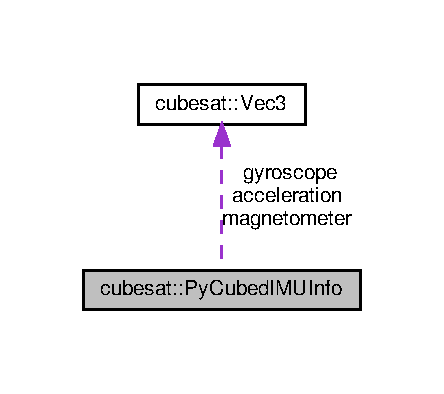
\includegraphics[width=213pt]{structcubesat_1_1PyCubedIMUInfo__coll__graph}
\end{center}
\end{figure}
\subsection*{Public Attributes}
\begin{DoxyCompactItemize}
\item 
double \hyperlink{structcubesat_1_1PyCubedIMUInfo_a3785744217caa5acc457d3f92cd07c7c}{utc}
\item 
\hyperlink{structcubesat_1_1Vec3}{Vec3} \hyperlink{structcubesat_1_1PyCubedIMUInfo_ad0340495c1ab66bb9060444541b33256}{magnetometer}
\item 
\hyperlink{structcubesat_1_1Vec3}{Vec3} \hyperlink{structcubesat_1_1PyCubedIMUInfo_a3b31df3109a4212dde3971da625dcb26}{acceleration}
\item 
\hyperlink{structcubesat_1_1Vec3}{Vec3} \hyperlink{structcubesat_1_1PyCubedIMUInfo_af053687ac00c0d374c092e9f39634756}{gyroscope}
\end{DoxyCompactItemize}


\subsection{Detailed Description}
Holds \hyperlink{classcubesat_1_1IMU}{I\+MU} information. 

\subsection{Member Data Documentation}
\mbox{\Hypertarget{structcubesat_1_1PyCubedIMUInfo_a3b31df3109a4212dde3971da625dcb26}\label{structcubesat_1_1PyCubedIMUInfo_a3b31df3109a4212dde3971da625dcb26}} 
\index{cubesat\+::\+Py\+Cubed\+I\+M\+U\+Info@{cubesat\+::\+Py\+Cubed\+I\+M\+U\+Info}!acceleration@{acceleration}}
\index{acceleration@{acceleration}!cubesat\+::\+Py\+Cubed\+I\+M\+U\+Info@{cubesat\+::\+Py\+Cubed\+I\+M\+U\+Info}}
\subsubsection{\texorpdfstring{acceleration}{acceleration}}
{\footnotesize\ttfamily \hyperlink{structcubesat_1_1Vec3}{Vec3} cubesat\+::\+Py\+Cubed\+I\+M\+U\+Info\+::acceleration}

\mbox{\Hypertarget{structcubesat_1_1PyCubedIMUInfo_af053687ac00c0d374c092e9f39634756}\label{structcubesat_1_1PyCubedIMUInfo_af053687ac00c0d374c092e9f39634756}} 
\index{cubesat\+::\+Py\+Cubed\+I\+M\+U\+Info@{cubesat\+::\+Py\+Cubed\+I\+M\+U\+Info}!gyroscope@{gyroscope}}
\index{gyroscope@{gyroscope}!cubesat\+::\+Py\+Cubed\+I\+M\+U\+Info@{cubesat\+::\+Py\+Cubed\+I\+M\+U\+Info}}
\subsubsection{\texorpdfstring{gyroscope}{gyroscope}}
{\footnotesize\ttfamily \hyperlink{structcubesat_1_1Vec3}{Vec3} cubesat\+::\+Py\+Cubed\+I\+M\+U\+Info\+::gyroscope}

\mbox{\Hypertarget{structcubesat_1_1PyCubedIMUInfo_ad0340495c1ab66bb9060444541b33256}\label{structcubesat_1_1PyCubedIMUInfo_ad0340495c1ab66bb9060444541b33256}} 
\index{cubesat\+::\+Py\+Cubed\+I\+M\+U\+Info@{cubesat\+::\+Py\+Cubed\+I\+M\+U\+Info}!magnetometer@{magnetometer}}
\index{magnetometer@{magnetometer}!cubesat\+::\+Py\+Cubed\+I\+M\+U\+Info@{cubesat\+::\+Py\+Cubed\+I\+M\+U\+Info}}
\subsubsection{\texorpdfstring{magnetometer}{magnetometer}}
{\footnotesize\ttfamily \hyperlink{structcubesat_1_1Vec3}{Vec3} cubesat\+::\+Py\+Cubed\+I\+M\+U\+Info\+::magnetometer}

\mbox{\Hypertarget{structcubesat_1_1PyCubedIMUInfo_a3785744217caa5acc457d3f92cd07c7c}\label{structcubesat_1_1PyCubedIMUInfo_a3785744217caa5acc457d3f92cd07c7c}} 
\index{cubesat\+::\+Py\+Cubed\+I\+M\+U\+Info@{cubesat\+::\+Py\+Cubed\+I\+M\+U\+Info}!utc@{utc}}
\index{utc@{utc}!cubesat\+::\+Py\+Cubed\+I\+M\+U\+Info@{cubesat\+::\+Py\+Cubed\+I\+M\+U\+Info}}
\subsubsection{\texorpdfstring{utc}{utc}}
{\footnotesize\ttfamily double cubesat\+::\+Py\+Cubed\+I\+M\+U\+Info\+::utc}



The documentation for this struct was generated from the following file\+:\begin{DoxyCompactItemize}
\item 
/home/osboxes/cosmos/source/projects/cubesat-\/kit/include/device/\hyperlink{PyCubedMessage_8h}{Py\+Cubed\+Message.\+h}\end{DoxyCompactItemize}

\hypertarget{structcubesat_1_1PyCubedPacket}{}\section{cubesat\+:\+:Py\+Cubed\+Packet Struct Reference}
\label{structcubesat_1_1PyCubedPacket}\index{cubesat\+::\+Py\+Cubed\+Packet@{cubesat\+::\+Py\+Cubed\+Packet}}


{\ttfamily \#include $<$Py\+Cubed\+Message.\+h$>$}



Collaboration diagram for cubesat\+:\+:Py\+Cubed\+Packet\+:\nopagebreak
\begin{figure}[H]
\begin{center}
\leavevmode
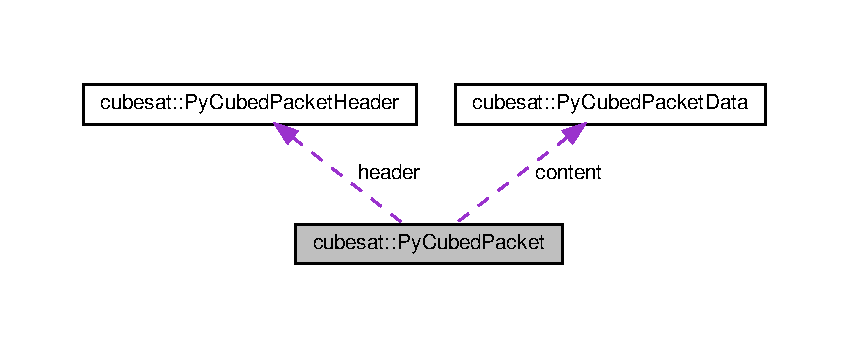
\includegraphics[width=350pt]{structcubesat_1_1PyCubedPacket__coll__graph}
\end{center}
\end{figure}
\subsection*{Public Attributes}
\begin{DoxyCompactItemize}
\item 
\hyperlink{structcubesat_1_1PyCubedPacketHeader}{Py\+Cubed\+Packet\+Header} \hyperlink{structcubesat_1_1PyCubedPacket_a3fee0058b22c1346c8d21b2985c6d49d}{header}
\item 
\hyperlink{structcubesat_1_1PyCubedPacketData}{Py\+Cubed\+Packet\+Data} \hyperlink{structcubesat_1_1PyCubedPacket_af33aeae9a8ae102140146acd32484ba0}{content}
\end{DoxyCompactItemize}


\subsection{Member Data Documentation}
\mbox{\Hypertarget{structcubesat_1_1PyCubedPacket_af33aeae9a8ae102140146acd32484ba0}\label{structcubesat_1_1PyCubedPacket_af33aeae9a8ae102140146acd32484ba0}} 
\index{cubesat\+::\+Py\+Cubed\+Packet@{cubesat\+::\+Py\+Cubed\+Packet}!content@{content}}
\index{content@{content}!cubesat\+::\+Py\+Cubed\+Packet@{cubesat\+::\+Py\+Cubed\+Packet}}
\subsubsection{\texorpdfstring{content}{content}}
{\footnotesize\ttfamily \hyperlink{structcubesat_1_1PyCubedPacketData}{Py\+Cubed\+Packet\+Data} cubesat\+::\+Py\+Cubed\+Packet\+::content}

\mbox{\Hypertarget{structcubesat_1_1PyCubedPacket_a3fee0058b22c1346c8d21b2985c6d49d}\label{structcubesat_1_1PyCubedPacket_a3fee0058b22c1346c8d21b2985c6d49d}} 
\index{cubesat\+::\+Py\+Cubed\+Packet@{cubesat\+::\+Py\+Cubed\+Packet}!header@{header}}
\index{header@{header}!cubesat\+::\+Py\+Cubed\+Packet@{cubesat\+::\+Py\+Cubed\+Packet}}
\subsubsection{\texorpdfstring{header}{header}}
{\footnotesize\ttfamily \hyperlink{structcubesat_1_1PyCubedPacketHeader}{Py\+Cubed\+Packet\+Header} cubesat\+::\+Py\+Cubed\+Packet\+::header}



The documentation for this struct was generated from the following file\+:\begin{DoxyCompactItemize}
\item 
/home/osboxes/cosmos/source/projects/cubesat-\/kit/include/device/\hyperlink{PyCubedMessage_8h}{Py\+Cubed\+Message.\+h}\end{DoxyCompactItemize}

\hypertarget{structcubesat_1_1PyCubedPacketData}{}\section{cubesat\+:\+:Py\+Cubed\+Packet\+Data Struct Reference}
\label{structcubesat_1_1PyCubedPacketData}\index{cubesat\+::\+Py\+Cubed\+Packet\+Data@{cubesat\+::\+Py\+Cubed\+Packet\+Data}}


{\ttfamily \#include $<$Py\+Cubed\+Message.\+h$>$}

\subsection*{Public Attributes}
\begin{DoxyCompactItemize}
\item 
\begin{tabbing}
xx\=xx\=xx\=xx\=xx\=xx\=xx\=xx\=xx\=\kill
union \{\\
\>uint8\_t \hyperlink{structcubesat_1_1PyCubedPacketData_ac838d716cfc7c6252dff158668b6291a}{id\_bytes} \mbox{[}2\mbox{]}\\
\>uint16\_t \hyperlink{structcubesat_1_1PyCubedPacketData_a02926763ed43d1a5fea510f63644b5cf}{message\_type\_id}\\
\}; \\

\end{tabbing}\item 
vector$<$ uint8\+\_\+t $>$ \hyperlink{structcubesat_1_1PyCubedPacketData_a078edbf1fbb4ca6a89a6bacb8e78cdc2}{data}
\end{DoxyCompactItemize}


\subsection{Member Data Documentation}
\mbox{\Hypertarget{structcubesat_1_1PyCubedPacketData_a6daf046ad7c04e04066aff8a637babb0}\label{structcubesat_1_1PyCubedPacketData_a6daf046ad7c04e04066aff8a637babb0}} 
\subsubsection{\texorpdfstring{"@16}{@16}}
{\footnotesize\ttfamily union \{ ... \} }

\mbox{\Hypertarget{structcubesat_1_1PyCubedPacketData_a078edbf1fbb4ca6a89a6bacb8e78cdc2}\label{structcubesat_1_1PyCubedPacketData_a078edbf1fbb4ca6a89a6bacb8e78cdc2}} 
\index{cubesat\+::\+Py\+Cubed\+Packet\+Data@{cubesat\+::\+Py\+Cubed\+Packet\+Data}!data@{data}}
\index{data@{data}!cubesat\+::\+Py\+Cubed\+Packet\+Data@{cubesat\+::\+Py\+Cubed\+Packet\+Data}}
\subsubsection{\texorpdfstring{data}{data}}
{\footnotesize\ttfamily vector$<$uint8\+\_\+t$>$ cubesat\+::\+Py\+Cubed\+Packet\+Data\+::data}

\mbox{\Hypertarget{structcubesat_1_1PyCubedPacketData_ac838d716cfc7c6252dff158668b6291a}\label{structcubesat_1_1PyCubedPacketData_ac838d716cfc7c6252dff158668b6291a}} 
\index{cubesat\+::\+Py\+Cubed\+Packet\+Data@{cubesat\+::\+Py\+Cubed\+Packet\+Data}!id\+\_\+bytes@{id\+\_\+bytes}}
\index{id\+\_\+bytes@{id\+\_\+bytes}!cubesat\+::\+Py\+Cubed\+Packet\+Data@{cubesat\+::\+Py\+Cubed\+Packet\+Data}}
\subsubsection{\texorpdfstring{id\+\_\+bytes}{id\_bytes}}
{\footnotesize\ttfamily uint8\+\_\+t cubesat\+::\+Py\+Cubed\+Packet\+Data\+::id\+\_\+bytes\mbox{[}2\mbox{]}}

\mbox{\Hypertarget{structcubesat_1_1PyCubedPacketData_a02926763ed43d1a5fea510f63644b5cf}\label{structcubesat_1_1PyCubedPacketData_a02926763ed43d1a5fea510f63644b5cf}} 
\index{cubesat\+::\+Py\+Cubed\+Packet\+Data@{cubesat\+::\+Py\+Cubed\+Packet\+Data}!message\+\_\+type\+\_\+id@{message\+\_\+type\+\_\+id}}
\index{message\+\_\+type\+\_\+id@{message\+\_\+type\+\_\+id}!cubesat\+::\+Py\+Cubed\+Packet\+Data@{cubesat\+::\+Py\+Cubed\+Packet\+Data}}
\subsubsection{\texorpdfstring{message\+\_\+type\+\_\+id}{message\_type\_id}}
{\footnotesize\ttfamily uint16\+\_\+t cubesat\+::\+Py\+Cubed\+Packet\+Data\+::message\+\_\+type\+\_\+id}



The documentation for this struct was generated from the following file\+:\begin{DoxyCompactItemize}
\item 
/home/osboxes/cosmos/source/projects/cubesat-\/kit/include/device/\hyperlink{PyCubedMessage_8h}{Py\+Cubed\+Message.\+h}\end{DoxyCompactItemize}

\hypertarget{structcubesat_1_1PyCubedPacketHeader}{}\section{cubesat\+:\+:Py\+Cubed\+Packet\+Header Struct Reference}
\label{structcubesat_1_1PyCubedPacketHeader}\index{cubesat\+::\+Py\+Cubed\+Packet\+Header@{cubesat\+::\+Py\+Cubed\+Packet\+Header}}


{\ttfamily \#include $<$Py\+Cubed\+Message.\+h$>$}

\subsection*{Public Attributes}
\begin{DoxyCompactItemize}
\item 
uint8\+\_\+t \hyperlink{structcubesat_1_1PyCubedPacketHeader_ac287aab87779442ad0b7920688586c8c}{bytes} \mbox{[}6\mbox{]}
\item 
\begin{tabbing}
xx\=xx\=xx\=xx\=xx\=xx\=xx\=xx\=xx\=\kill
struct \{\\
\>unsigned \hyperlink{structcubesat_1_1PyCubedPacketHeader_a254cda485af31555d5ebbf1474c5e6c1}{packet\_version\_number}: 3\\
\>unsigned \hyperlink{structcubesat_1_1PyCubedPacketHeader_ab6dad7185cd28250ff37b256774ea6a1}{packet\_type}: 1\\
\>unsigned \hyperlink{structcubesat_1_1PyCubedPacketHeader_a8b449583c7a24ac7cf6b9b29dc63af7a}{secondary\_header\_flag}: 1\\
\>unsigned \hyperlink{structcubesat_1_1PyCubedPacketHeader_a3b3581160add43f191c6a6859a557c5d}{apid}: 11\\
\>unsigned \hyperlink{structcubesat_1_1PyCubedPacketHeader_a4c803d383516d016a6aa0bea290af55e}{sequence\_flags}: 2\\
\>unsigned \hyperlink{structcubesat_1_1PyCubedPacketHeader_a95a52681056d84fcd39c97e949d3ac57}{sequence\_count}: 14\\
\>unsigned \hyperlink{structcubesat_1_1PyCubedPacketHeader_ad1c206c2f7073dad5b97d7bb26e041b8}{packet\_data\_length}: 16\\
\} \hyperlink{structcubesat_1_1PyCubedPacketHeader_aa1bc03af9a992257c0a19b0a5c596001}{fields}\\

\end{tabbing}\end{DoxyCompactItemize}


\subsection{Member Data Documentation}
\mbox{\Hypertarget{structcubesat_1_1PyCubedPacketHeader_a3b3581160add43f191c6a6859a557c5d}\label{structcubesat_1_1PyCubedPacketHeader_a3b3581160add43f191c6a6859a557c5d}} 
\index{cubesat\+::\+Py\+Cubed\+Packet\+Header@{cubesat\+::\+Py\+Cubed\+Packet\+Header}!apid@{apid}}
\index{apid@{apid}!cubesat\+::\+Py\+Cubed\+Packet\+Header@{cubesat\+::\+Py\+Cubed\+Packet\+Header}}
\subsubsection{\texorpdfstring{apid}{apid}}
{\footnotesize\ttfamily unsigned cubesat\+::\+Py\+Cubed\+Packet\+Header\+::apid}

\mbox{\Hypertarget{structcubesat_1_1PyCubedPacketHeader_ac287aab87779442ad0b7920688586c8c}\label{structcubesat_1_1PyCubedPacketHeader_ac287aab87779442ad0b7920688586c8c}} 
\index{cubesat\+::\+Py\+Cubed\+Packet\+Header@{cubesat\+::\+Py\+Cubed\+Packet\+Header}!bytes@{bytes}}
\index{bytes@{bytes}!cubesat\+::\+Py\+Cubed\+Packet\+Header@{cubesat\+::\+Py\+Cubed\+Packet\+Header}}
\subsubsection{\texorpdfstring{bytes}{bytes}}
{\footnotesize\ttfamily uint8\+\_\+t cubesat\+::\+Py\+Cubed\+Packet\+Header\+::bytes\mbox{[}6\mbox{]}}

\mbox{\Hypertarget{structcubesat_1_1PyCubedPacketHeader_aa1bc03af9a992257c0a19b0a5c596001}\label{structcubesat_1_1PyCubedPacketHeader_aa1bc03af9a992257c0a19b0a5c596001}} 
\index{cubesat\+::\+Py\+Cubed\+Packet\+Header@{cubesat\+::\+Py\+Cubed\+Packet\+Header}!fields@{fields}}
\index{fields@{fields}!cubesat\+::\+Py\+Cubed\+Packet\+Header@{cubesat\+::\+Py\+Cubed\+Packet\+Header}}
\subsubsection{\texorpdfstring{fields}{fields}}
{\footnotesize\ttfamily struct \{ ... \}   cubesat\+::\+Py\+Cubed\+Packet\+Header\+::fields}

\mbox{\Hypertarget{structcubesat_1_1PyCubedPacketHeader_ad1c206c2f7073dad5b97d7bb26e041b8}\label{structcubesat_1_1PyCubedPacketHeader_ad1c206c2f7073dad5b97d7bb26e041b8}} 
\index{cubesat\+::\+Py\+Cubed\+Packet\+Header@{cubesat\+::\+Py\+Cubed\+Packet\+Header}!packet\+\_\+data\+\_\+length@{packet\+\_\+data\+\_\+length}}
\index{packet\+\_\+data\+\_\+length@{packet\+\_\+data\+\_\+length}!cubesat\+::\+Py\+Cubed\+Packet\+Header@{cubesat\+::\+Py\+Cubed\+Packet\+Header}}
\subsubsection{\texorpdfstring{packet\+\_\+data\+\_\+length}{packet\_data\_length}}
{\footnotesize\ttfamily unsigned cubesat\+::\+Py\+Cubed\+Packet\+Header\+::packet\+\_\+data\+\_\+length}

\mbox{\Hypertarget{structcubesat_1_1PyCubedPacketHeader_ab6dad7185cd28250ff37b256774ea6a1}\label{structcubesat_1_1PyCubedPacketHeader_ab6dad7185cd28250ff37b256774ea6a1}} 
\index{cubesat\+::\+Py\+Cubed\+Packet\+Header@{cubesat\+::\+Py\+Cubed\+Packet\+Header}!packet\+\_\+type@{packet\+\_\+type}}
\index{packet\+\_\+type@{packet\+\_\+type}!cubesat\+::\+Py\+Cubed\+Packet\+Header@{cubesat\+::\+Py\+Cubed\+Packet\+Header}}
\subsubsection{\texorpdfstring{packet\+\_\+type}{packet\_type}}
{\footnotesize\ttfamily unsigned cubesat\+::\+Py\+Cubed\+Packet\+Header\+::packet\+\_\+type}

\mbox{\Hypertarget{structcubesat_1_1PyCubedPacketHeader_a254cda485af31555d5ebbf1474c5e6c1}\label{structcubesat_1_1PyCubedPacketHeader_a254cda485af31555d5ebbf1474c5e6c1}} 
\index{cubesat\+::\+Py\+Cubed\+Packet\+Header@{cubesat\+::\+Py\+Cubed\+Packet\+Header}!packet\+\_\+version\+\_\+number@{packet\+\_\+version\+\_\+number}}
\index{packet\+\_\+version\+\_\+number@{packet\+\_\+version\+\_\+number}!cubesat\+::\+Py\+Cubed\+Packet\+Header@{cubesat\+::\+Py\+Cubed\+Packet\+Header}}
\subsubsection{\texorpdfstring{packet\+\_\+version\+\_\+number}{packet\_version\_number}}
{\footnotesize\ttfamily unsigned cubesat\+::\+Py\+Cubed\+Packet\+Header\+::packet\+\_\+version\+\_\+number}

\mbox{\Hypertarget{structcubesat_1_1PyCubedPacketHeader_a8b449583c7a24ac7cf6b9b29dc63af7a}\label{structcubesat_1_1PyCubedPacketHeader_a8b449583c7a24ac7cf6b9b29dc63af7a}} 
\index{cubesat\+::\+Py\+Cubed\+Packet\+Header@{cubesat\+::\+Py\+Cubed\+Packet\+Header}!secondary\+\_\+header\+\_\+flag@{secondary\+\_\+header\+\_\+flag}}
\index{secondary\+\_\+header\+\_\+flag@{secondary\+\_\+header\+\_\+flag}!cubesat\+::\+Py\+Cubed\+Packet\+Header@{cubesat\+::\+Py\+Cubed\+Packet\+Header}}
\subsubsection{\texorpdfstring{secondary\+\_\+header\+\_\+flag}{secondary\_header\_flag}}
{\footnotesize\ttfamily unsigned cubesat\+::\+Py\+Cubed\+Packet\+Header\+::secondary\+\_\+header\+\_\+flag}

\mbox{\Hypertarget{structcubesat_1_1PyCubedPacketHeader_a95a52681056d84fcd39c97e949d3ac57}\label{structcubesat_1_1PyCubedPacketHeader_a95a52681056d84fcd39c97e949d3ac57}} 
\index{cubesat\+::\+Py\+Cubed\+Packet\+Header@{cubesat\+::\+Py\+Cubed\+Packet\+Header}!sequence\+\_\+count@{sequence\+\_\+count}}
\index{sequence\+\_\+count@{sequence\+\_\+count}!cubesat\+::\+Py\+Cubed\+Packet\+Header@{cubesat\+::\+Py\+Cubed\+Packet\+Header}}
\subsubsection{\texorpdfstring{sequence\+\_\+count}{sequence\_count}}
{\footnotesize\ttfamily unsigned cubesat\+::\+Py\+Cubed\+Packet\+Header\+::sequence\+\_\+count}

\mbox{\Hypertarget{structcubesat_1_1PyCubedPacketHeader_a4c803d383516d016a6aa0bea290af55e}\label{structcubesat_1_1PyCubedPacketHeader_a4c803d383516d016a6aa0bea290af55e}} 
\index{cubesat\+::\+Py\+Cubed\+Packet\+Header@{cubesat\+::\+Py\+Cubed\+Packet\+Header}!sequence\+\_\+flags@{sequence\+\_\+flags}}
\index{sequence\+\_\+flags@{sequence\+\_\+flags}!cubesat\+::\+Py\+Cubed\+Packet\+Header@{cubesat\+::\+Py\+Cubed\+Packet\+Header}}
\subsubsection{\texorpdfstring{sequence\+\_\+flags}{sequence\_flags}}
{\footnotesize\ttfamily unsigned cubesat\+::\+Py\+Cubed\+Packet\+Header\+::sequence\+\_\+flags}



The documentation for this struct was generated from the following file\+:\begin{DoxyCompactItemize}
\item 
/home/osboxes/cosmos/source/projects/cubesat-\/kit/include/device/\hyperlink{PyCubedMessage_8h}{Py\+Cubed\+Message.\+h}\end{DoxyCompactItemize}

\hypertarget{structcubesat_1_1PyCubedPowerInfo}{}\section{cubesat\+:\+:Py\+Cubed\+Power\+Info Struct Reference}
\label{structcubesat_1_1PyCubedPowerInfo}\index{cubesat\+::\+Py\+Cubed\+Power\+Info@{cubesat\+::\+Py\+Cubed\+Power\+Info}}


Holds power information.  




{\ttfamily \#include $<$Py\+Cubed\+Message.\+h$>$}

\subsection*{Public Attributes}
\begin{DoxyCompactItemize}
\item 
double \hyperlink{structcubesat_1_1PyCubedPowerInfo_a996ed40659fdb6b6839be93c41916823}{utc}
\item 
float \hyperlink{structcubesat_1_1PyCubedPowerInfo_ac55dcd441743ca47a9c0f928f9786a04}{batt\+\_\+voltage}
\item 
float \hyperlink{structcubesat_1_1PyCubedPowerInfo_a1982f742645b1901fdc1fe3ce655f3cf}{batt\+\_\+current}
\item 
float \hyperlink{structcubesat_1_1PyCubedPowerInfo_a7ed9543532030de641e198378f1eca8c}{sys\+\_\+voltage}
\item 
float \hyperlink{structcubesat_1_1PyCubedPowerInfo_ad424fe069fc2306e899192f1a8a95a3a}{sys\+\_\+current}
\end{DoxyCompactItemize}


\subsection{Detailed Description}
Holds power information. 

\subsection{Member Data Documentation}
\mbox{\Hypertarget{structcubesat_1_1PyCubedPowerInfo_a1982f742645b1901fdc1fe3ce655f3cf}\label{structcubesat_1_1PyCubedPowerInfo_a1982f742645b1901fdc1fe3ce655f3cf}} 
\index{cubesat\+::\+Py\+Cubed\+Power\+Info@{cubesat\+::\+Py\+Cubed\+Power\+Info}!batt\+\_\+current@{batt\+\_\+current}}
\index{batt\+\_\+current@{batt\+\_\+current}!cubesat\+::\+Py\+Cubed\+Power\+Info@{cubesat\+::\+Py\+Cubed\+Power\+Info}}
\subsubsection{\texorpdfstring{batt\+\_\+current}{batt\_current}}
{\footnotesize\ttfamily float cubesat\+::\+Py\+Cubed\+Power\+Info\+::batt\+\_\+current}

\mbox{\Hypertarget{structcubesat_1_1PyCubedPowerInfo_ac55dcd441743ca47a9c0f928f9786a04}\label{structcubesat_1_1PyCubedPowerInfo_ac55dcd441743ca47a9c0f928f9786a04}} 
\index{cubesat\+::\+Py\+Cubed\+Power\+Info@{cubesat\+::\+Py\+Cubed\+Power\+Info}!batt\+\_\+voltage@{batt\+\_\+voltage}}
\index{batt\+\_\+voltage@{batt\+\_\+voltage}!cubesat\+::\+Py\+Cubed\+Power\+Info@{cubesat\+::\+Py\+Cubed\+Power\+Info}}
\subsubsection{\texorpdfstring{batt\+\_\+voltage}{batt\_voltage}}
{\footnotesize\ttfamily float cubesat\+::\+Py\+Cubed\+Power\+Info\+::batt\+\_\+voltage}

\mbox{\Hypertarget{structcubesat_1_1PyCubedPowerInfo_ad424fe069fc2306e899192f1a8a95a3a}\label{structcubesat_1_1PyCubedPowerInfo_ad424fe069fc2306e899192f1a8a95a3a}} 
\index{cubesat\+::\+Py\+Cubed\+Power\+Info@{cubesat\+::\+Py\+Cubed\+Power\+Info}!sys\+\_\+current@{sys\+\_\+current}}
\index{sys\+\_\+current@{sys\+\_\+current}!cubesat\+::\+Py\+Cubed\+Power\+Info@{cubesat\+::\+Py\+Cubed\+Power\+Info}}
\subsubsection{\texorpdfstring{sys\+\_\+current}{sys\_current}}
{\footnotesize\ttfamily float cubesat\+::\+Py\+Cubed\+Power\+Info\+::sys\+\_\+current}

\mbox{\Hypertarget{structcubesat_1_1PyCubedPowerInfo_a7ed9543532030de641e198378f1eca8c}\label{structcubesat_1_1PyCubedPowerInfo_a7ed9543532030de641e198378f1eca8c}} 
\index{cubesat\+::\+Py\+Cubed\+Power\+Info@{cubesat\+::\+Py\+Cubed\+Power\+Info}!sys\+\_\+voltage@{sys\+\_\+voltage}}
\index{sys\+\_\+voltage@{sys\+\_\+voltage}!cubesat\+::\+Py\+Cubed\+Power\+Info@{cubesat\+::\+Py\+Cubed\+Power\+Info}}
\subsubsection{\texorpdfstring{sys\+\_\+voltage}{sys\_voltage}}
{\footnotesize\ttfamily float cubesat\+::\+Py\+Cubed\+Power\+Info\+::sys\+\_\+voltage}

\mbox{\Hypertarget{structcubesat_1_1PyCubedPowerInfo_a996ed40659fdb6b6839be93c41916823}\label{structcubesat_1_1PyCubedPowerInfo_a996ed40659fdb6b6839be93c41916823}} 
\index{cubesat\+::\+Py\+Cubed\+Power\+Info@{cubesat\+::\+Py\+Cubed\+Power\+Info}!utc@{utc}}
\index{utc@{utc}!cubesat\+::\+Py\+Cubed\+Power\+Info@{cubesat\+::\+Py\+Cubed\+Power\+Info}}
\subsubsection{\texorpdfstring{utc}{utc}}
{\footnotesize\ttfamily double cubesat\+::\+Py\+Cubed\+Power\+Info\+::utc}



The documentation for this struct was generated from the following file\+:\begin{DoxyCompactItemize}
\item 
/home/osboxes/cosmos/source/projects/cubesat-\/kit/include/device/\hyperlink{PyCubedMessage_8h}{Py\+Cubed\+Message.\+h}\end{DoxyCompactItemize}

\hypertarget{structcubesat_1_1PyCubedTempInfo}{}\section{cubesat\+:\+:Py\+Cubed\+Temp\+Info Struct Reference}
\label{structcubesat_1_1PyCubedTempInfo}\index{cubesat\+::\+Py\+Cubed\+Temp\+Info@{cubesat\+::\+Py\+Cubed\+Temp\+Info}}


Holds temperature information.  




{\ttfamily \#include $<$Py\+Cubed\+Message.\+h$>$}

\subsection*{Public Attributes}
\begin{DoxyCompactItemize}
\item 
double \hyperlink{structcubesat_1_1PyCubedTempInfo_aa2e137388f0e71ddc9f8f528ec66dd20}{utc}
\item 
float \hyperlink{structcubesat_1_1PyCubedTempInfo_ae0773ca752df2cd590263f0a8d39e404}{cpu\+\_\+temp}
\item 
float \hyperlink{structcubesat_1_1PyCubedTempInfo_ae92b48f3a454931d8653e5b81904363a}{batt\+\_\+temp}
\end{DoxyCompactItemize}


\subsection{Detailed Description}
Holds temperature information. 

\subsection{Member Data Documentation}
\mbox{\Hypertarget{structcubesat_1_1PyCubedTempInfo_ae92b48f3a454931d8653e5b81904363a}\label{structcubesat_1_1PyCubedTempInfo_ae92b48f3a454931d8653e5b81904363a}} 
\index{cubesat\+::\+Py\+Cubed\+Temp\+Info@{cubesat\+::\+Py\+Cubed\+Temp\+Info}!batt\+\_\+temp@{batt\+\_\+temp}}
\index{batt\+\_\+temp@{batt\+\_\+temp}!cubesat\+::\+Py\+Cubed\+Temp\+Info@{cubesat\+::\+Py\+Cubed\+Temp\+Info}}
\subsubsection{\texorpdfstring{batt\+\_\+temp}{batt\_temp}}
{\footnotesize\ttfamily float cubesat\+::\+Py\+Cubed\+Temp\+Info\+::batt\+\_\+temp}

\mbox{\Hypertarget{structcubesat_1_1PyCubedTempInfo_ae0773ca752df2cd590263f0a8d39e404}\label{structcubesat_1_1PyCubedTempInfo_ae0773ca752df2cd590263f0a8d39e404}} 
\index{cubesat\+::\+Py\+Cubed\+Temp\+Info@{cubesat\+::\+Py\+Cubed\+Temp\+Info}!cpu\+\_\+temp@{cpu\+\_\+temp}}
\index{cpu\+\_\+temp@{cpu\+\_\+temp}!cubesat\+::\+Py\+Cubed\+Temp\+Info@{cubesat\+::\+Py\+Cubed\+Temp\+Info}}
\subsubsection{\texorpdfstring{cpu\+\_\+temp}{cpu\_temp}}
{\footnotesize\ttfamily float cubesat\+::\+Py\+Cubed\+Temp\+Info\+::cpu\+\_\+temp}

\mbox{\Hypertarget{structcubesat_1_1PyCubedTempInfo_aa2e137388f0e71ddc9f8f528ec66dd20}\label{structcubesat_1_1PyCubedTempInfo_aa2e137388f0e71ddc9f8f528ec66dd20}} 
\index{cubesat\+::\+Py\+Cubed\+Temp\+Info@{cubesat\+::\+Py\+Cubed\+Temp\+Info}!utc@{utc}}
\index{utc@{utc}!cubesat\+::\+Py\+Cubed\+Temp\+Info@{cubesat\+::\+Py\+Cubed\+Temp\+Info}}
\subsubsection{\texorpdfstring{utc}{utc}}
{\footnotesize\ttfamily double cubesat\+::\+Py\+Cubed\+Temp\+Info\+::utc}



The documentation for this struct was generated from the following file\+:\begin{DoxyCompactItemize}
\item 
/home/osboxes/cosmos/source/projects/cubesat-\/kit/include/device/\hyperlink{PyCubedMessage_8h}{Py\+Cubed\+Message.\+h}\end{DoxyCompactItemize}

\hypertarget{classcubesat_1_1RadioTransceiver}{}\section{cubesat\+:\+:Radio\+Transceiver Class Reference}
\label{classcubesat_1_1RadioTransceiver}\index{cubesat\+::\+Radio\+Transceiver@{cubesat\+::\+Radio\+Transceiver}}


{\ttfamily \#include $<$Device.\+h$>$}



Inheritance diagram for cubesat\+:\+:Radio\+Transceiver\+:
\nopagebreak
\begin{figure}[H]
\begin{center}
\leavevmode
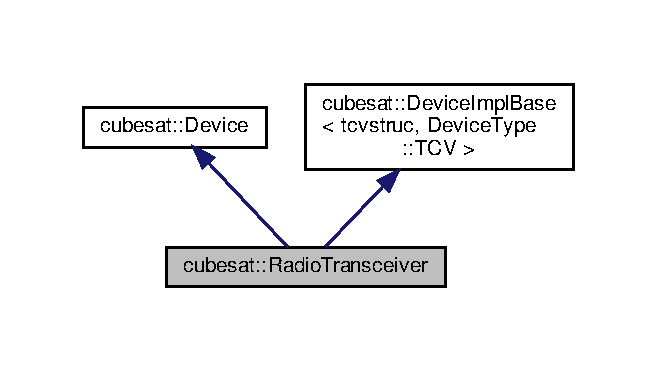
\includegraphics[width=316pt]{classcubesat_1_1RadioTransceiver__inherit__graph}
\end{center}
\end{figure}


Collaboration diagram for cubesat\+:\+:Radio\+Transceiver\+:
\nopagebreak
\begin{figure}[H]
\begin{center}
\leavevmode
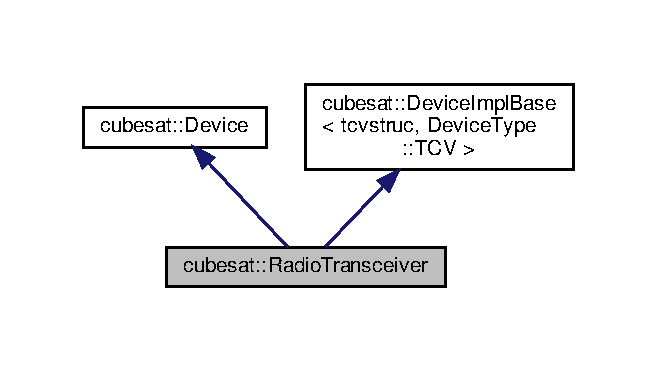
\includegraphics[width=316pt]{classcubesat_1_1RadioTransceiver__coll__graph}
\end{center}
\end{figure}
\subsection*{Public Member Functions}
\begin{DoxyCompactItemize}
\item 
\hyperlink{classcubesat_1_1RadioTransceiver_af785e8d80b098be752539b404186e6cb}{Radio\+Transceiver} (Agent $\ast$\hyperlink{classcubesat_1_1Device_a8499108eccaf7375bea8ead0182391a6}{agent}, int \hyperlink{classcubesat_1_1Device_a1deca725b01f8ef37e49662da6db4e53}{cindex}, int \hyperlink{classcubesat_1_1Device_a8a2b3d6d7400e6796c31705058172982}{dindex})
\item 
virtual \hyperlink{classcubesat_1_1RadioTransceiver_a30988a36b57334c7c24131e1dd1660c0}{$\sim$\+Radio\+Transceiver} ()
\item 
\hyperlink{classcubesat_1_1RadioTransceiver_a580041b634b8ad24443d07e7172977d1}{\+\_\+\+Add\+Property} (temperature, temp)
\item 
\hyperlink{classcubesat_1_1RadioTransceiver_af0269bd98075bf8c19086c107c99c326}{\+\_\+\+Add\+Property} (utc, utc)
\item 
\hyperlink{classcubesat_1_1RadioTransceiver_ae432428cd51ab4dde0bd48da09dcbcb3}{\+\_\+\+Add\+Property} (voltage, volt)
\item 
\hyperlink{classcubesat_1_1RadioTransceiver_ada909dbdb331b383d49952708ed238d7}{\+\_\+\+Add\+Property} (current, amp)
\item 
\hyperlink{classcubesat_1_1RadioTransceiver_a5c3926cb67019211e57ab3a4ef63aa5c}{\+\_\+\+Add\+Property} (power, power)
\item 
\hyperlink{classcubesat_1_1RadioTransceiver_aebed815b814e4e9f88b09d6e2c1a7edb}{\+\_\+\+Add\+Property} (enabled, enabled)
\item 
\hyperlink{classcubesat_1_1RadioTransceiver_a0bd1b6445940d545762f38297cbab769}{\+\_\+\+Add\+Property} (frequency, freq)
\item 
\hyperlink{classcubesat_1_1RadioTransceiver_a304006511eb06938617869b722153a97}{\+\_\+\+Add\+Property} (max\+\_\+frequency, maxfreq)
\item 
\hyperlink{classcubesat_1_1RadioTransceiver_ac7816dfb616ed0730e7f5f0a360bd087}{\+\_\+\+Add\+Property} (min\+\_\+frequency, minfreq)
\item 
\hyperlink{classcubesat_1_1RadioTransceiver_a0862d47cb9a6d2a1144f04a151213ebd}{\+\_\+\+Add\+Property} (power\+\_\+in, powerin)
\item 
\hyperlink{classcubesat_1_1RadioTransceiver_a2f726171eefc33d423083d6efe8f6701}{\+\_\+\+Add\+Property} (power\+\_\+out, powerout)
\item 
\hyperlink{classcubesat_1_1RadioTransceiver_a20d8b9573699dbbd3852d4833ee8e68f}{\+\_\+\+Add\+Property} (max\+\_\+power, maxpower)
\item 
\hyperlink{classcubesat_1_1RadioTransceiver_a6063051de0ead97cca2dd6bf47a63a53}{\+\_\+\+Add\+Property} (bandwidth, band)
\item 
\hyperlink{classcubesat_1_1RadioTransceiver_a1e06f3051377b0df184021daca19475a}{\+\_\+\+Add\+Property} (good\+\_\+packet\+\_\+count, goodcnt)
\item 
\hyperlink{classcubesat_1_1RadioTransceiver_adae4d603a281ba18f4fd0f7583f43371}{\+\_\+\+Add\+Property} (bad\+\_\+packet\+\_\+count, badcnt)
\end{DoxyCompactItemize}
\subsection*{Additional Inherited Members}


\subsection{Constructor \& Destructor Documentation}
\mbox{\Hypertarget{classcubesat_1_1RadioTransceiver_af785e8d80b098be752539b404186e6cb}\label{classcubesat_1_1RadioTransceiver_af785e8d80b098be752539b404186e6cb}} 
\index{cubesat\+::\+Radio\+Transceiver@{cubesat\+::\+Radio\+Transceiver}!Radio\+Transceiver@{Radio\+Transceiver}}
\index{Radio\+Transceiver@{Radio\+Transceiver}!cubesat\+::\+Radio\+Transceiver@{cubesat\+::\+Radio\+Transceiver}}
\subsubsection{\texorpdfstring{Radio\+Transceiver()}{RadioTransceiver()}}
{\footnotesize\ttfamily cubesat\+::\+Radio\+Transceiver\+::\+Radio\+Transceiver (\begin{DoxyParamCaption}\item[{Agent $\ast$}]{agent,  }\item[{int}]{cindex,  }\item[{int}]{dindex }\end{DoxyParamCaption})\hspace{0.3cm}{\ttfamily [inline]}}

\mbox{\Hypertarget{classcubesat_1_1RadioTransceiver_a30988a36b57334c7c24131e1dd1660c0}\label{classcubesat_1_1RadioTransceiver_a30988a36b57334c7c24131e1dd1660c0}} 
\index{cubesat\+::\+Radio\+Transceiver@{cubesat\+::\+Radio\+Transceiver}!````~Radio\+Transceiver@{$\sim$\+Radio\+Transceiver}}
\index{````~Radio\+Transceiver@{$\sim$\+Radio\+Transceiver}!cubesat\+::\+Radio\+Transceiver@{cubesat\+::\+Radio\+Transceiver}}
\subsubsection{\texorpdfstring{$\sim$\+Radio\+Transceiver()}{~RadioTransceiver()}}
{\footnotesize\ttfamily virtual cubesat\+::\+Radio\+Transceiver\+::$\sim$\+Radio\+Transceiver (\begin{DoxyParamCaption}{ }\end{DoxyParamCaption})\hspace{0.3cm}{\ttfamily [inline]}, {\ttfamily [virtual]}}



\subsection{Member Function Documentation}
\mbox{\Hypertarget{classcubesat_1_1RadioTransceiver_a580041b634b8ad24443d07e7172977d1}\label{classcubesat_1_1RadioTransceiver_a580041b634b8ad24443d07e7172977d1}} 
\index{cubesat\+::\+Radio\+Transceiver@{cubesat\+::\+Radio\+Transceiver}!\+\_\+\+Add\+Property@{\+\_\+\+Add\+Property}}
\index{\+\_\+\+Add\+Property@{\+\_\+\+Add\+Property}!cubesat\+::\+Radio\+Transceiver@{cubesat\+::\+Radio\+Transceiver}}
\subsubsection{\texorpdfstring{\+\_\+\+Add\+Property()}{\_AddProperty()}\hspace{0.1cm}{\footnotesize\ttfamily [1/15]}}
{\footnotesize\ttfamily cubesat\+::\+Radio\+Transceiver\+::\+\_\+\+Add\+Property (\begin{DoxyParamCaption}\item[{temperature}]{,  }\item[{temp}]{ }\end{DoxyParamCaption})}

\mbox{\Hypertarget{classcubesat_1_1RadioTransceiver_af0269bd98075bf8c19086c107c99c326}\label{classcubesat_1_1RadioTransceiver_af0269bd98075bf8c19086c107c99c326}} 
\index{cubesat\+::\+Radio\+Transceiver@{cubesat\+::\+Radio\+Transceiver}!\+\_\+\+Add\+Property@{\+\_\+\+Add\+Property}}
\index{\+\_\+\+Add\+Property@{\+\_\+\+Add\+Property}!cubesat\+::\+Radio\+Transceiver@{cubesat\+::\+Radio\+Transceiver}}
\subsubsection{\texorpdfstring{\+\_\+\+Add\+Property()}{\_AddProperty()}\hspace{0.1cm}{\footnotesize\ttfamily [2/15]}}
{\footnotesize\ttfamily cubesat\+::\+Radio\+Transceiver\+::\+\_\+\+Add\+Property (\begin{DoxyParamCaption}\item[{utc}]{,  }\item[{utc}]{ }\end{DoxyParamCaption})}

\mbox{\Hypertarget{classcubesat_1_1RadioTransceiver_ae432428cd51ab4dde0bd48da09dcbcb3}\label{classcubesat_1_1RadioTransceiver_ae432428cd51ab4dde0bd48da09dcbcb3}} 
\index{cubesat\+::\+Radio\+Transceiver@{cubesat\+::\+Radio\+Transceiver}!\+\_\+\+Add\+Property@{\+\_\+\+Add\+Property}}
\index{\+\_\+\+Add\+Property@{\+\_\+\+Add\+Property}!cubesat\+::\+Radio\+Transceiver@{cubesat\+::\+Radio\+Transceiver}}
\subsubsection{\texorpdfstring{\+\_\+\+Add\+Property()}{\_AddProperty()}\hspace{0.1cm}{\footnotesize\ttfamily [3/15]}}
{\footnotesize\ttfamily cubesat\+::\+Radio\+Transceiver\+::\+\_\+\+Add\+Property (\begin{DoxyParamCaption}\item[{voltage}]{,  }\item[{volt}]{ }\end{DoxyParamCaption})}

\mbox{\Hypertarget{classcubesat_1_1RadioTransceiver_ada909dbdb331b383d49952708ed238d7}\label{classcubesat_1_1RadioTransceiver_ada909dbdb331b383d49952708ed238d7}} 
\index{cubesat\+::\+Radio\+Transceiver@{cubesat\+::\+Radio\+Transceiver}!\+\_\+\+Add\+Property@{\+\_\+\+Add\+Property}}
\index{\+\_\+\+Add\+Property@{\+\_\+\+Add\+Property}!cubesat\+::\+Radio\+Transceiver@{cubesat\+::\+Radio\+Transceiver}}
\subsubsection{\texorpdfstring{\+\_\+\+Add\+Property()}{\_AddProperty()}\hspace{0.1cm}{\footnotesize\ttfamily [4/15]}}
{\footnotesize\ttfamily cubesat\+::\+Radio\+Transceiver\+::\+\_\+\+Add\+Property (\begin{DoxyParamCaption}\item[{current}]{,  }\item[{amp}]{ }\end{DoxyParamCaption})}

\mbox{\Hypertarget{classcubesat_1_1RadioTransceiver_a5c3926cb67019211e57ab3a4ef63aa5c}\label{classcubesat_1_1RadioTransceiver_a5c3926cb67019211e57ab3a4ef63aa5c}} 
\index{cubesat\+::\+Radio\+Transceiver@{cubesat\+::\+Radio\+Transceiver}!\+\_\+\+Add\+Property@{\+\_\+\+Add\+Property}}
\index{\+\_\+\+Add\+Property@{\+\_\+\+Add\+Property}!cubesat\+::\+Radio\+Transceiver@{cubesat\+::\+Radio\+Transceiver}}
\subsubsection{\texorpdfstring{\+\_\+\+Add\+Property()}{\_AddProperty()}\hspace{0.1cm}{\footnotesize\ttfamily [5/15]}}
{\footnotesize\ttfamily cubesat\+::\+Radio\+Transceiver\+::\+\_\+\+Add\+Property (\begin{DoxyParamCaption}\item[{power}]{,  }\item[{power}]{ }\end{DoxyParamCaption})}

\mbox{\Hypertarget{classcubesat_1_1RadioTransceiver_aebed815b814e4e9f88b09d6e2c1a7edb}\label{classcubesat_1_1RadioTransceiver_aebed815b814e4e9f88b09d6e2c1a7edb}} 
\index{cubesat\+::\+Radio\+Transceiver@{cubesat\+::\+Radio\+Transceiver}!\+\_\+\+Add\+Property@{\+\_\+\+Add\+Property}}
\index{\+\_\+\+Add\+Property@{\+\_\+\+Add\+Property}!cubesat\+::\+Radio\+Transceiver@{cubesat\+::\+Radio\+Transceiver}}
\subsubsection{\texorpdfstring{\+\_\+\+Add\+Property()}{\_AddProperty()}\hspace{0.1cm}{\footnotesize\ttfamily [6/15]}}
{\footnotesize\ttfamily cubesat\+::\+Radio\+Transceiver\+::\+\_\+\+Add\+Property (\begin{DoxyParamCaption}\item[{enabled}]{,  }\item[{enabled}]{ }\end{DoxyParamCaption})}

\mbox{\Hypertarget{classcubesat_1_1RadioTransceiver_a0bd1b6445940d545762f38297cbab769}\label{classcubesat_1_1RadioTransceiver_a0bd1b6445940d545762f38297cbab769}} 
\index{cubesat\+::\+Radio\+Transceiver@{cubesat\+::\+Radio\+Transceiver}!\+\_\+\+Add\+Property@{\+\_\+\+Add\+Property}}
\index{\+\_\+\+Add\+Property@{\+\_\+\+Add\+Property}!cubesat\+::\+Radio\+Transceiver@{cubesat\+::\+Radio\+Transceiver}}
\subsubsection{\texorpdfstring{\+\_\+\+Add\+Property()}{\_AddProperty()}\hspace{0.1cm}{\footnotesize\ttfamily [7/15]}}
{\footnotesize\ttfamily cubesat\+::\+Radio\+Transceiver\+::\+\_\+\+Add\+Property (\begin{DoxyParamCaption}\item[{frequency}]{,  }\item[{freq}]{ }\end{DoxyParamCaption})}

\mbox{\Hypertarget{classcubesat_1_1RadioTransceiver_a304006511eb06938617869b722153a97}\label{classcubesat_1_1RadioTransceiver_a304006511eb06938617869b722153a97}} 
\index{cubesat\+::\+Radio\+Transceiver@{cubesat\+::\+Radio\+Transceiver}!\+\_\+\+Add\+Property@{\+\_\+\+Add\+Property}}
\index{\+\_\+\+Add\+Property@{\+\_\+\+Add\+Property}!cubesat\+::\+Radio\+Transceiver@{cubesat\+::\+Radio\+Transceiver}}
\subsubsection{\texorpdfstring{\+\_\+\+Add\+Property()}{\_AddProperty()}\hspace{0.1cm}{\footnotesize\ttfamily [8/15]}}
{\footnotesize\ttfamily cubesat\+::\+Radio\+Transceiver\+::\+\_\+\+Add\+Property (\begin{DoxyParamCaption}\item[{max\+\_\+frequency}]{,  }\item[{maxfreq}]{ }\end{DoxyParamCaption})}

\mbox{\Hypertarget{classcubesat_1_1RadioTransceiver_ac7816dfb616ed0730e7f5f0a360bd087}\label{classcubesat_1_1RadioTransceiver_ac7816dfb616ed0730e7f5f0a360bd087}} 
\index{cubesat\+::\+Radio\+Transceiver@{cubesat\+::\+Radio\+Transceiver}!\+\_\+\+Add\+Property@{\+\_\+\+Add\+Property}}
\index{\+\_\+\+Add\+Property@{\+\_\+\+Add\+Property}!cubesat\+::\+Radio\+Transceiver@{cubesat\+::\+Radio\+Transceiver}}
\subsubsection{\texorpdfstring{\+\_\+\+Add\+Property()}{\_AddProperty()}\hspace{0.1cm}{\footnotesize\ttfamily [9/15]}}
{\footnotesize\ttfamily cubesat\+::\+Radio\+Transceiver\+::\+\_\+\+Add\+Property (\begin{DoxyParamCaption}\item[{min\+\_\+frequency}]{,  }\item[{minfreq}]{ }\end{DoxyParamCaption})}

\mbox{\Hypertarget{classcubesat_1_1RadioTransceiver_a0862d47cb9a6d2a1144f04a151213ebd}\label{classcubesat_1_1RadioTransceiver_a0862d47cb9a6d2a1144f04a151213ebd}} 
\index{cubesat\+::\+Radio\+Transceiver@{cubesat\+::\+Radio\+Transceiver}!\+\_\+\+Add\+Property@{\+\_\+\+Add\+Property}}
\index{\+\_\+\+Add\+Property@{\+\_\+\+Add\+Property}!cubesat\+::\+Radio\+Transceiver@{cubesat\+::\+Radio\+Transceiver}}
\subsubsection{\texorpdfstring{\+\_\+\+Add\+Property()}{\_AddProperty()}\hspace{0.1cm}{\footnotesize\ttfamily [10/15]}}
{\footnotesize\ttfamily cubesat\+::\+Radio\+Transceiver\+::\+\_\+\+Add\+Property (\begin{DoxyParamCaption}\item[{power\+\_\+in}]{,  }\item[{powerin}]{ }\end{DoxyParamCaption})}

\mbox{\Hypertarget{classcubesat_1_1RadioTransceiver_a2f726171eefc33d423083d6efe8f6701}\label{classcubesat_1_1RadioTransceiver_a2f726171eefc33d423083d6efe8f6701}} 
\index{cubesat\+::\+Radio\+Transceiver@{cubesat\+::\+Radio\+Transceiver}!\+\_\+\+Add\+Property@{\+\_\+\+Add\+Property}}
\index{\+\_\+\+Add\+Property@{\+\_\+\+Add\+Property}!cubesat\+::\+Radio\+Transceiver@{cubesat\+::\+Radio\+Transceiver}}
\subsubsection{\texorpdfstring{\+\_\+\+Add\+Property()}{\_AddProperty()}\hspace{0.1cm}{\footnotesize\ttfamily [11/15]}}
{\footnotesize\ttfamily cubesat\+::\+Radio\+Transceiver\+::\+\_\+\+Add\+Property (\begin{DoxyParamCaption}\item[{power\+\_\+out}]{,  }\item[{powerout}]{ }\end{DoxyParamCaption})}

\mbox{\Hypertarget{classcubesat_1_1RadioTransceiver_a20d8b9573699dbbd3852d4833ee8e68f}\label{classcubesat_1_1RadioTransceiver_a20d8b9573699dbbd3852d4833ee8e68f}} 
\index{cubesat\+::\+Radio\+Transceiver@{cubesat\+::\+Radio\+Transceiver}!\+\_\+\+Add\+Property@{\+\_\+\+Add\+Property}}
\index{\+\_\+\+Add\+Property@{\+\_\+\+Add\+Property}!cubesat\+::\+Radio\+Transceiver@{cubesat\+::\+Radio\+Transceiver}}
\subsubsection{\texorpdfstring{\+\_\+\+Add\+Property()}{\_AddProperty()}\hspace{0.1cm}{\footnotesize\ttfamily [12/15]}}
{\footnotesize\ttfamily cubesat\+::\+Radio\+Transceiver\+::\+\_\+\+Add\+Property (\begin{DoxyParamCaption}\item[{max\+\_\+power}]{,  }\item[{maxpower}]{ }\end{DoxyParamCaption})}

\mbox{\Hypertarget{classcubesat_1_1RadioTransceiver_a6063051de0ead97cca2dd6bf47a63a53}\label{classcubesat_1_1RadioTransceiver_a6063051de0ead97cca2dd6bf47a63a53}} 
\index{cubesat\+::\+Radio\+Transceiver@{cubesat\+::\+Radio\+Transceiver}!\+\_\+\+Add\+Property@{\+\_\+\+Add\+Property}}
\index{\+\_\+\+Add\+Property@{\+\_\+\+Add\+Property}!cubesat\+::\+Radio\+Transceiver@{cubesat\+::\+Radio\+Transceiver}}
\subsubsection{\texorpdfstring{\+\_\+\+Add\+Property()}{\_AddProperty()}\hspace{0.1cm}{\footnotesize\ttfamily [13/15]}}
{\footnotesize\ttfamily cubesat\+::\+Radio\+Transceiver\+::\+\_\+\+Add\+Property (\begin{DoxyParamCaption}\item[{bandwidth}]{,  }\item[{band}]{ }\end{DoxyParamCaption})}

\mbox{\Hypertarget{classcubesat_1_1RadioTransceiver_a1e06f3051377b0df184021daca19475a}\label{classcubesat_1_1RadioTransceiver_a1e06f3051377b0df184021daca19475a}} 
\index{cubesat\+::\+Radio\+Transceiver@{cubesat\+::\+Radio\+Transceiver}!\+\_\+\+Add\+Property@{\+\_\+\+Add\+Property}}
\index{\+\_\+\+Add\+Property@{\+\_\+\+Add\+Property}!cubesat\+::\+Radio\+Transceiver@{cubesat\+::\+Radio\+Transceiver}}
\subsubsection{\texorpdfstring{\+\_\+\+Add\+Property()}{\_AddProperty()}\hspace{0.1cm}{\footnotesize\ttfamily [14/15]}}
{\footnotesize\ttfamily cubesat\+::\+Radio\+Transceiver\+::\+\_\+\+Add\+Property (\begin{DoxyParamCaption}\item[{good\+\_\+packet\+\_\+count}]{,  }\item[{goodcnt}]{ }\end{DoxyParamCaption})}

\mbox{\Hypertarget{classcubesat_1_1RadioTransceiver_adae4d603a281ba18f4fd0f7583f43371}\label{classcubesat_1_1RadioTransceiver_adae4d603a281ba18f4fd0f7583f43371}} 
\index{cubesat\+::\+Radio\+Transceiver@{cubesat\+::\+Radio\+Transceiver}!\+\_\+\+Add\+Property@{\+\_\+\+Add\+Property}}
\index{\+\_\+\+Add\+Property@{\+\_\+\+Add\+Property}!cubesat\+::\+Radio\+Transceiver@{cubesat\+::\+Radio\+Transceiver}}
\subsubsection{\texorpdfstring{\+\_\+\+Add\+Property()}{\_AddProperty()}\hspace{0.1cm}{\footnotesize\ttfamily [15/15]}}
{\footnotesize\ttfamily cubesat\+::\+Radio\+Transceiver\+::\+\_\+\+Add\+Property (\begin{DoxyParamCaption}\item[{bad\+\_\+packet\+\_\+count}]{,  }\item[{badcnt}]{ }\end{DoxyParamCaption})}



The documentation for this class was generated from the following file\+:\begin{DoxyCompactItemize}
\item 
/home/osboxes/cosmos/source/projects/cubesat-\/kit/include/utility/\hyperlink{Device_8h}{Device.\+h}\end{DoxyCompactItemize}

\hypertarget{classcubesat_1_1RaspberryPi}{}\section{cubesat\+:\+:Raspberry\+Pi Class Reference}
\label{classcubesat_1_1RaspberryPi}\index{cubesat\+::\+Raspberry\+Pi@{cubesat\+::\+Raspberry\+Pi}}


{\ttfamily \#include $<$Raspberry\+Pi.\+h$>$}

\subsection*{Public Member Functions}
\begin{DoxyCompactItemize}
\item 
void \hyperlink{classcubesat_1_1RaspberryPi_a6d6fea9ced78884cf1e8beb2a0f9b2f4}{Send\+File} (const std\+::string \&src, const std\+::string \&dest)
\begin{DoxyCompactList}\small\item\em Uses rsync to synchronize source file with destination file. \end{DoxyCompactList}\end{DoxyCompactItemize}


\subsection{Member Function Documentation}
\mbox{\Hypertarget{classcubesat_1_1RaspberryPi_a6d6fea9ced78884cf1e8beb2a0f9b2f4}\label{classcubesat_1_1RaspberryPi_a6d6fea9ced78884cf1e8beb2a0f9b2f4}} 
\index{cubesat\+::\+Raspberry\+Pi@{cubesat\+::\+Raspberry\+Pi}!Send\+File@{Send\+File}}
\index{Send\+File@{Send\+File}!cubesat\+::\+Raspberry\+Pi@{cubesat\+::\+Raspberry\+Pi}}
\subsubsection{\texorpdfstring{Send\+File()}{SendFile()}}
{\footnotesize\ttfamily void cubesat\+::\+Raspberry\+Pi\+::\+Send\+File (\begin{DoxyParamCaption}\item[{const std\+::string \&}]{src,  }\item[{const std\+::string \&}]{dest }\end{DoxyParamCaption})}



Uses rsync to synchronize source file with destination file. 


\begin{DoxyParams}{Parameters}
{\em src} & The source file \\
\hline
{\em dest} & The destination file \\
\hline
\end{DoxyParams}


The documentation for this class was generated from the following file\+:\begin{DoxyCompactItemize}
\item 
/home/osboxes/cosmos/source/projects/cubesat-\/kit/include/device/\hyperlink{RaspberryPi_8h}{Raspberry\+Pi.\+h}\end{DoxyCompactItemize}

\hypertarget{classcubesat_1_1RemoteAgent}{}\section{cubesat\+:\+:Remote\+Agent Class Reference}
\label{classcubesat_1_1RemoteAgent}\index{cubesat\+::\+Remote\+Agent@{cubesat\+::\+Remote\+Agent}}


A utility class for communicating with agents on seperate processes.  




{\ttfamily \#include $<$Remote\+Agent.\+h$>$}

\subsection*{Public Member Functions}
\begin{DoxyCompactItemize}
\item 
\hyperlink{classcubesat_1_1RemoteAgent_a011f3eddd537166c854dc976f6e04f9b}{Remote\+Agent} ()
\item 
\hyperlink{classcubesat_1_1RemoteAgent_a415c6e6434cbc15c3e0b889c02efbe0a}{Remote\+Agent} (const std\+::string \&\hyperlink{classcubesat_1_1RemoteAgent_ad53ce2f7c8bbe8e8582f82740d5c38fe}{node\+\_\+name}, const std\+::string \&\hyperlink{classcubesat_1_1RemoteAgent_a11c308db5679e300962e8a79b875dba5}{agent\+\_\+name}, Agent $\ast$\hyperlink{classcubesat_1_1RemoteAgent_ab6ebf279927e308af1ecaf81782af2a3}{agent}, beatstruc \hyperlink{classcubesat_1_1RemoteAgent_a56c2e7d52e3ebe7dfe69c4a779f1a375}{beat})
\item 
bool \hyperlink{classcubesat_1_1RemoteAgent_a149ba4f966974d78c265a18921057a6f}{Is\+Open} () const
\begin{DoxyCompactList}\small\item\em Checks if this agent was connected to successfully. \end{DoxyCompactList}\item 
bool \hyperlink{classcubesat_1_1RemoteAgent_a144dbf2aaccbe8cb53f811db1b62cea4}{Connect} (float wait\+\_\+sec=2.\+0f, bool crash\+\_\+if\+\_\+failed=false)
\begin{DoxyCompactList}\small\item\em Attempts to connect to the remote agent. \end{DoxyCompactList}\item 
std\+::unordered\+\_\+map$<$ std\+::string, Json\+::\+Value $>$ \hyperlink{classcubesat_1_1RemoteAgent_afaaaec695eae602bc2a84d6ad88ed7f6}{Get\+C\+O\+S\+M\+O\+S\+Values} (std\+::vector$<$ std\+::string $>$ keys)
\begin{DoxyCompactList}\small\item\em Gets a list of state of health values from a remote agent. \end{DoxyCompactList}\item 
{\footnotesize template$<$typename... Properties, typename... Args$>$ }\\std\+::unordered\+\_\+map$<$ std\+::string, std\+::string $>$ \hyperlink{classcubesat_1_1RemoteAgent_a08ff2ce8cd3114533ea51959f3f8c9ef}{Get\+Properties} (Args... device\+\_\+names\+\_\+)
\item 
{\footnotesize template$<$typename... Args$>$ }\\std\+::string \hyperlink{classcubesat_1_1RemoteAgent_a480b864cabc5b9f5b69833a3bc1c1d2f}{Send\+Request} (std\+::string request\+\_\+name, Args... args)
\begin{DoxyCompactList}\small\item\em Sends a request to the remote agent. \end{DoxyCompactList}\end{DoxyCompactItemize}
\subsection*{Protected Attributes}
\begin{DoxyCompactItemize}
\item 
Agent $\ast$ \hyperlink{classcubesat_1_1RemoteAgent_ab6ebf279927e308af1ecaf81782af2a3}{agent}
\begin{DoxyCompactList}\small\item\em The non-\/remote agent. \end{DoxyCompactList}\item 
beatstruc \hyperlink{classcubesat_1_1RemoteAgent_a56c2e7d52e3ebe7dfe69c4a779f1a375}{beat}
\begin{DoxyCompactList}\small\item\em The heartbeat of the remote agent. \end{DoxyCompactList}\item 
float \hyperlink{classcubesat_1_1RemoteAgent_a22d81c0c42adb6cef33cdef627631f43}{wait\+\_\+time} = 5.\+0f
\begin{DoxyCompactList}\small\item\em The timeout for requests. \end{DoxyCompactList}\item 
std\+::string \hyperlink{classcubesat_1_1RemoteAgent_ad53ce2f7c8bbe8e8582f82740d5c38fe}{node\+\_\+name}
\begin{DoxyCompactList}\small\item\em The name of the node the remote agent is on. \end{DoxyCompactList}\item 
std\+::string \hyperlink{classcubesat_1_1RemoteAgent_a11c308db5679e300962e8a79b875dba5}{agent\+\_\+name}
\begin{DoxyCompactList}\small\item\em The name of the remote agent. \end{DoxyCompactList}\end{DoxyCompactItemize}


\subsection{Detailed Description}
A utility class for communicating with agents on seperate processes. 

\subsection{Constructor \& Destructor Documentation}
\mbox{\Hypertarget{classcubesat_1_1RemoteAgent_a011f3eddd537166c854dc976f6e04f9b}\label{classcubesat_1_1RemoteAgent_a011f3eddd537166c854dc976f6e04f9b}} 
\index{cubesat\+::\+Remote\+Agent@{cubesat\+::\+Remote\+Agent}!Remote\+Agent@{Remote\+Agent}}
\index{Remote\+Agent@{Remote\+Agent}!cubesat\+::\+Remote\+Agent@{cubesat\+::\+Remote\+Agent}}
\subsubsection{\texorpdfstring{Remote\+Agent()}{RemoteAgent()}\hspace{0.1cm}{\footnotesize\ttfamily [1/2]}}
{\footnotesize\ttfamily cubesat\+::\+Remote\+Agent\+::\+Remote\+Agent (\begin{DoxyParamCaption}{ }\end{DoxyParamCaption})\hspace{0.3cm}{\ttfamily [inline]}}

\mbox{\Hypertarget{classcubesat_1_1RemoteAgent_a415c6e6434cbc15c3e0b889c02efbe0a}\label{classcubesat_1_1RemoteAgent_a415c6e6434cbc15c3e0b889c02efbe0a}} 
\index{cubesat\+::\+Remote\+Agent@{cubesat\+::\+Remote\+Agent}!Remote\+Agent@{Remote\+Agent}}
\index{Remote\+Agent@{Remote\+Agent}!cubesat\+::\+Remote\+Agent@{cubesat\+::\+Remote\+Agent}}
\subsubsection{\texorpdfstring{Remote\+Agent()}{RemoteAgent()}\hspace{0.1cm}{\footnotesize\ttfamily [2/2]}}
{\footnotesize\ttfamily cubesat\+::\+Remote\+Agent\+::\+Remote\+Agent (\begin{DoxyParamCaption}\item[{const std\+::string \&}]{node\+\_\+name,  }\item[{const std\+::string \&}]{agent\+\_\+name,  }\item[{Agent $\ast$}]{agent,  }\item[{beatstruc}]{beat }\end{DoxyParamCaption})\hspace{0.3cm}{\ttfamily [inline]}}



\subsection{Member Function Documentation}
\mbox{\Hypertarget{classcubesat_1_1RemoteAgent_a144dbf2aaccbe8cb53f811db1b62cea4}\label{classcubesat_1_1RemoteAgent_a144dbf2aaccbe8cb53f811db1b62cea4}} 
\index{cubesat\+::\+Remote\+Agent@{cubesat\+::\+Remote\+Agent}!Connect@{Connect}}
\index{Connect@{Connect}!cubesat\+::\+Remote\+Agent@{cubesat\+::\+Remote\+Agent}}
\subsubsection{\texorpdfstring{Connect()}{Connect()}}
{\footnotesize\ttfamily bool cubesat\+::\+Remote\+Agent\+::\+Connect (\begin{DoxyParamCaption}\item[{float}]{wait\+\_\+sec = {\ttfamily 2.0f},  }\item[{bool}]{crash\+\_\+if\+\_\+failed = {\ttfamily false} }\end{DoxyParamCaption})\hspace{0.3cm}{\ttfamily [inline]}}



Attempts to connect to the remote agent. 


\begin{DoxyParams}{Parameters}
{\em wait\+\_\+sec} & The maximum duration in seconds to wait \\
\hline
{\em crash\+\_\+if\+\_\+failed} & If true, the program will crash if the agent is not found \\
\hline
\end{DoxyParams}
\begin{DoxyReturn}{Returns}
True if the agent connected successfully 
\end{DoxyReturn}
\mbox{\Hypertarget{classcubesat_1_1RemoteAgent_afaaaec695eae602bc2a84d6ad88ed7f6}\label{classcubesat_1_1RemoteAgent_afaaaec695eae602bc2a84d6ad88ed7f6}} 
\index{cubesat\+::\+Remote\+Agent@{cubesat\+::\+Remote\+Agent}!Get\+C\+O\+S\+M\+O\+S\+Values@{Get\+C\+O\+S\+M\+O\+S\+Values}}
\index{Get\+C\+O\+S\+M\+O\+S\+Values@{Get\+C\+O\+S\+M\+O\+S\+Values}!cubesat\+::\+Remote\+Agent@{cubesat\+::\+Remote\+Agent}}
\subsubsection{\texorpdfstring{Get\+C\+O\+S\+M\+O\+S\+Values()}{GetCOSMOSValues()}}
{\footnotesize\ttfamily std\+::unordered\+\_\+map$<$std\+::string, Json\+::\+Value$>$ cubesat\+::\+Remote\+Agent\+::\+Get\+C\+O\+S\+M\+O\+S\+Values (\begin{DoxyParamCaption}\item[{std\+::vector$<$ std\+::string $>$}]{keys }\end{DoxyParamCaption})\hspace{0.3cm}{\ttfamily [inline]}}



Gets a list of state of health values from a remote agent. 


\begin{DoxyParams}{Parameters}
{\em keys} & A vector of C\+O\+S\+M\+OS namespace names to retrieve \\
\hline
\end{DoxyParams}
\begin{DoxyReturn}{Returns}
A table of values, indexed by the given keys 
\end{DoxyReturn}
\mbox{\Hypertarget{classcubesat_1_1RemoteAgent_a08ff2ce8cd3114533ea51959f3f8c9ef}\label{classcubesat_1_1RemoteAgent_a08ff2ce8cd3114533ea51959f3f8c9ef}} 
\index{cubesat\+::\+Remote\+Agent@{cubesat\+::\+Remote\+Agent}!Get\+Properties@{Get\+Properties}}
\index{Get\+Properties@{Get\+Properties}!cubesat\+::\+Remote\+Agent@{cubesat\+::\+Remote\+Agent}}
\subsubsection{\texorpdfstring{Get\+Properties()}{GetProperties()}}
{\footnotesize\ttfamily template$<$typename... Properties, typename... Args$>$ \\
std\+::unordered\+\_\+map$<$std\+::string, std\+::string$>$ cubesat\+::\+Remote\+Agent\+::\+Get\+Properties (\begin{DoxyParamCaption}\item[{Args...}]{device\+\_\+names\+\_\+ }\end{DoxyParamCaption})\hspace{0.3cm}{\ttfamily [inline]}}

\mbox{\Hypertarget{classcubesat_1_1RemoteAgent_a149ba4f966974d78c265a18921057a6f}\label{classcubesat_1_1RemoteAgent_a149ba4f966974d78c265a18921057a6f}} 
\index{cubesat\+::\+Remote\+Agent@{cubesat\+::\+Remote\+Agent}!Is\+Open@{Is\+Open}}
\index{Is\+Open@{Is\+Open}!cubesat\+::\+Remote\+Agent@{cubesat\+::\+Remote\+Agent}}
\subsubsection{\texorpdfstring{Is\+Open()}{IsOpen()}}
{\footnotesize\ttfamily bool cubesat\+::\+Remote\+Agent\+::\+Is\+Open (\begin{DoxyParamCaption}{ }\end{DoxyParamCaption}) const\hspace{0.3cm}{\ttfamily [inline]}}



Checks if this agent was connected to successfully. 

\begin{DoxyReturn}{Returns}
True if connected 
\end{DoxyReturn}
\mbox{\Hypertarget{classcubesat_1_1RemoteAgent_a480b864cabc5b9f5b69833a3bc1c1d2f}\label{classcubesat_1_1RemoteAgent_a480b864cabc5b9f5b69833a3bc1c1d2f}} 
\index{cubesat\+::\+Remote\+Agent@{cubesat\+::\+Remote\+Agent}!Send\+Request@{Send\+Request}}
\index{Send\+Request@{Send\+Request}!cubesat\+::\+Remote\+Agent@{cubesat\+::\+Remote\+Agent}}
\subsubsection{\texorpdfstring{Send\+Request()}{SendRequest()}}
{\footnotesize\ttfamily template$<$typename... Args$>$ \\
std\+::string cubesat\+::\+Remote\+Agent\+::\+Send\+Request (\begin{DoxyParamCaption}\item[{std\+::string}]{request\+\_\+name,  }\item[{Args...}]{args }\end{DoxyParamCaption})\hspace{0.3cm}{\ttfamily [inline]}}



Sends a request to the remote agent. 


\begin{DoxyParams}{Parameters}
{\em request\+\_\+name} & The name of the request \\
\hline
{\em args} & The arguments to the request \\
\hline
\end{DoxyParams}
\begin{DoxyReturn}{Returns}
The response, or an empty string on failure 
\end{DoxyReturn}


\subsection{Member Data Documentation}
\mbox{\Hypertarget{classcubesat_1_1RemoteAgent_ab6ebf279927e308af1ecaf81782af2a3}\label{classcubesat_1_1RemoteAgent_ab6ebf279927e308af1ecaf81782af2a3}} 
\index{cubesat\+::\+Remote\+Agent@{cubesat\+::\+Remote\+Agent}!agent@{agent}}
\index{agent@{agent}!cubesat\+::\+Remote\+Agent@{cubesat\+::\+Remote\+Agent}}
\subsubsection{\texorpdfstring{agent}{agent}}
{\footnotesize\ttfamily Agent$\ast$ cubesat\+::\+Remote\+Agent\+::agent\hspace{0.3cm}{\ttfamily [protected]}}



The non-\/remote agent. 

\mbox{\Hypertarget{classcubesat_1_1RemoteAgent_a11c308db5679e300962e8a79b875dba5}\label{classcubesat_1_1RemoteAgent_a11c308db5679e300962e8a79b875dba5}} 
\index{cubesat\+::\+Remote\+Agent@{cubesat\+::\+Remote\+Agent}!agent\+\_\+name@{agent\+\_\+name}}
\index{agent\+\_\+name@{agent\+\_\+name}!cubesat\+::\+Remote\+Agent@{cubesat\+::\+Remote\+Agent}}
\subsubsection{\texorpdfstring{agent\+\_\+name}{agent\_name}}
{\footnotesize\ttfamily std\+::string cubesat\+::\+Remote\+Agent\+::agent\+\_\+name\hspace{0.3cm}{\ttfamily [protected]}}



The name of the remote agent. 

\mbox{\Hypertarget{classcubesat_1_1RemoteAgent_a56c2e7d52e3ebe7dfe69c4a779f1a375}\label{classcubesat_1_1RemoteAgent_a56c2e7d52e3ebe7dfe69c4a779f1a375}} 
\index{cubesat\+::\+Remote\+Agent@{cubesat\+::\+Remote\+Agent}!beat@{beat}}
\index{beat@{beat}!cubesat\+::\+Remote\+Agent@{cubesat\+::\+Remote\+Agent}}
\subsubsection{\texorpdfstring{beat}{beat}}
{\footnotesize\ttfamily beatstruc cubesat\+::\+Remote\+Agent\+::beat\hspace{0.3cm}{\ttfamily [protected]}}



The heartbeat of the remote agent. 

\mbox{\Hypertarget{classcubesat_1_1RemoteAgent_ad53ce2f7c8bbe8e8582f82740d5c38fe}\label{classcubesat_1_1RemoteAgent_ad53ce2f7c8bbe8e8582f82740d5c38fe}} 
\index{cubesat\+::\+Remote\+Agent@{cubesat\+::\+Remote\+Agent}!node\+\_\+name@{node\+\_\+name}}
\index{node\+\_\+name@{node\+\_\+name}!cubesat\+::\+Remote\+Agent@{cubesat\+::\+Remote\+Agent}}
\subsubsection{\texorpdfstring{node\+\_\+name}{node\_name}}
{\footnotesize\ttfamily std\+::string cubesat\+::\+Remote\+Agent\+::node\+\_\+name\hspace{0.3cm}{\ttfamily [protected]}}



The name of the node the remote agent is on. 

\mbox{\Hypertarget{classcubesat_1_1RemoteAgent_a22d81c0c42adb6cef33cdef627631f43}\label{classcubesat_1_1RemoteAgent_a22d81c0c42adb6cef33cdef627631f43}} 
\index{cubesat\+::\+Remote\+Agent@{cubesat\+::\+Remote\+Agent}!wait\+\_\+time@{wait\+\_\+time}}
\index{wait\+\_\+time@{wait\+\_\+time}!cubesat\+::\+Remote\+Agent@{cubesat\+::\+Remote\+Agent}}
\subsubsection{\texorpdfstring{wait\+\_\+time}{wait\_time}}
{\footnotesize\ttfamily float cubesat\+::\+Remote\+Agent\+::wait\+\_\+time = 5.\+0f\hspace{0.3cm}{\ttfamily [protected]}}



The timeout for requests. 



The documentation for this class was generated from the following file\+:\begin{DoxyCompactItemize}
\item 
/home/osboxes/cosmos/source/projects/cubesat-\/kit/include/utility/\hyperlink{RemoteAgent_8h}{Remote\+Agent.\+h}\end{DoxyCompactItemize}

\hypertarget{unioncubesat_1_1OPT3001_1_1ResultData}{}\section{cubesat\+:\+:O\+P\+T3001\+:\+:Result\+Data Union Reference}
\label{unioncubesat_1_1OPT3001_1_1ResultData}\index{cubesat\+::\+O\+P\+T3001\+::\+Result\+Data@{cubesat\+::\+O\+P\+T3001\+::\+Result\+Data}}


Stores data pulled from the result register.  




{\ttfamily \#include $<$O\+P\+T3001.\+h$>$}

\subsection*{Public Attributes}
\begin{DoxyCompactItemize}
\item 
uint16\+\_\+t \hyperlink{unioncubesat_1_1OPT3001_1_1ResultData_a5ea98dd31e38211d159635b818bff4f7}{raw\+\_\+data}
\item 
\begin{tabbing}
xx\=xx\=xx\=xx\=xx\=xx\=xx\=xx\=xx\=\kill
struct \{\\
\>uint16\_t \hyperlink{unioncubesat_1_1OPT3001_1_1ResultData_ac5479564c6231cfb6701b1dd5e411d01}{result}: 12\\
\>uint8\_t \hyperlink{unioncubesat_1_1OPT3001_1_1ResultData_acfca7cad4bdd0488cde78fc3944d6465}{exponent}: 4\\
\}; \\

\end{tabbing}\end{DoxyCompactItemize}


\subsection{Detailed Description}
Stores data pulled from the result register. 

\subsection{Member Data Documentation}
\mbox{\Hypertarget{unioncubesat_1_1OPT3001_1_1ResultData_ad760501899e98d60c7d0f5763b0a1c54}\label{unioncubesat_1_1OPT3001_1_1ResultData_ad760501899e98d60c7d0f5763b0a1c54}} 
\subsubsection{\texorpdfstring{"@13}{@13}}
{\footnotesize\ttfamily struct \{ ... \} }

\mbox{\Hypertarget{unioncubesat_1_1OPT3001_1_1ResultData_acfca7cad4bdd0488cde78fc3944d6465}\label{unioncubesat_1_1OPT3001_1_1ResultData_acfca7cad4bdd0488cde78fc3944d6465}} 
\index{cubesat\+::\+O\+P\+T3001\+::\+Result\+Data@{cubesat\+::\+O\+P\+T3001\+::\+Result\+Data}!exponent@{exponent}}
\index{exponent@{exponent}!cubesat\+::\+O\+P\+T3001\+::\+Result\+Data@{cubesat\+::\+O\+P\+T3001\+::\+Result\+Data}}
\subsubsection{\texorpdfstring{exponent}{exponent}}
{\footnotesize\ttfamily uint8\+\_\+t cubesat\+::\+O\+P\+T3001\+::\+Result\+Data\+::exponent}

\mbox{\Hypertarget{unioncubesat_1_1OPT3001_1_1ResultData_a5ea98dd31e38211d159635b818bff4f7}\label{unioncubesat_1_1OPT3001_1_1ResultData_a5ea98dd31e38211d159635b818bff4f7}} 
\index{cubesat\+::\+O\+P\+T3001\+::\+Result\+Data@{cubesat\+::\+O\+P\+T3001\+::\+Result\+Data}!raw\+\_\+data@{raw\+\_\+data}}
\index{raw\+\_\+data@{raw\+\_\+data}!cubesat\+::\+O\+P\+T3001\+::\+Result\+Data@{cubesat\+::\+O\+P\+T3001\+::\+Result\+Data}}
\subsubsection{\texorpdfstring{raw\+\_\+data}{raw\_data}}
{\footnotesize\ttfamily uint16\+\_\+t cubesat\+::\+O\+P\+T3001\+::\+Result\+Data\+::raw\+\_\+data}

\mbox{\Hypertarget{unioncubesat_1_1OPT3001_1_1ResultData_ac5479564c6231cfb6701b1dd5e411d01}\label{unioncubesat_1_1OPT3001_1_1ResultData_ac5479564c6231cfb6701b1dd5e411d01}} 
\index{cubesat\+::\+O\+P\+T3001\+::\+Result\+Data@{cubesat\+::\+O\+P\+T3001\+::\+Result\+Data}!result@{result}}
\index{result@{result}!cubesat\+::\+O\+P\+T3001\+::\+Result\+Data@{cubesat\+::\+O\+P\+T3001\+::\+Result\+Data}}
\subsubsection{\texorpdfstring{result}{result}}
{\footnotesize\ttfamily uint16\+\_\+t cubesat\+::\+O\+P\+T3001\+::\+Result\+Data\+::result}



The documentation for this union was generated from the following file\+:\begin{DoxyCompactItemize}
\item 
/home/osboxes/cosmos/source/projects/cubesat-\/kit/include/device/\hyperlink{OPT3001_8h}{O\+P\+T3001.\+h}\end{DoxyCompactItemize}

\hypertarget{classcubesat_1_1SimpleAgent}{}\section{cubesat\+:\+:Simple\+Agent Class Reference}
\label{classcubesat_1_1SimpleAgent}\index{cubesat\+::\+Simple\+Agent@{cubesat\+::\+Simple\+Agent}}


You guessed it -- it\textquotesingle{}s a simple agent.  




{\ttfamily \#include $<$Simple\+Agent.\+h$>$}



Inheritance diagram for cubesat\+:\+:Simple\+Agent\+:\nopagebreak
\begin{figure}[H]
\begin{center}
\leavevmode
\includegraphics[width=193pt]{classcubesat_1_1SimpleAgent__inherit__graph}
\end{center}
\end{figure}


Collaboration diagram for cubesat\+:\+:Simple\+Agent\+:\nopagebreak
\begin{figure}[H]
\begin{center}
\leavevmode
\includegraphics[width=251pt]{classcubesat_1_1SimpleAgent__coll__graph}
\end{center}
\end{figure}
\subsection*{Classes}
\begin{DoxyCompactItemize}
\item 
struct \hyperlink{structcubesat_1_1SimpleAgent_1_1ArgumentedRequestData}{Argumented\+Request\+Data}
\begin{DoxyCompactList}\small\item\em Stores data for a request with arguments. \end{DoxyCompactList}\item 
struct \hyperlink{structcubesat_1_1SimpleAgent_1_1NodeProperty}{Node\+Property}
\begin{DoxyCompactList}\small\item\em Represents a C\+O\+S\+M\+OS node property. \end{DoxyCompactList}\item 
struct \hyperlink{structcubesat_1_1SimpleAgent_1_1NonArgumentedRequestData}{Non\+Argumented\+Request\+Data}
\begin{DoxyCompactList}\small\item\em Stores data for a request with no arguments. \end{DoxyCompactList}\end{DoxyCompactItemize}
\subsection*{Public Member Functions}
\begin{DoxyCompactItemize}
\item 
\hyperlink{classcubesat_1_1SimpleAgent_a3ebec0e4954f90ecc14c0f964868ce4f}{Simple\+Agent} (const std\+::string \&name, std\+::string node=\hyperlink{cubesat__defs_8h_adce46043c3a8fc68eaee12044efd08e2}{C\+U\+B\+E\+S\+A\+T\+\_\+\+N\+O\+D\+E\+\_\+\+N\+A\+ME}, bool crash\+\_\+if\+\_\+not\+\_\+open=\hyperlink{SimpleAgent_8h_ae0458b189260d62b7f199e0324dc3cc4}{S\+I\+M\+P\+L\+E\+A\+G\+E\+N\+T\+\_\+\+S\+T\+R\+I\+C\+T\+\_\+\+M\+O\+DE})
\begin{DoxyCompactList}\small\item\em Creates a new simple agent with the given name. Don\textquotesingle{}t create multiple instances in one program! \end{DoxyCompactList}\item 
\hyperlink{classcubesat_1_1SimpleAgent_a000fb5fee9de4738ce05c74fb6756ada}{Simple\+Agent} (const \hyperlink{classcubesat_1_1SimpleAgent}{Simple\+Agent} \&)=delete
\begin{DoxyCompactList}\small\item\em Disallow copy construction for safety. \end{DoxyCompactList}\item 
virtual \hyperlink{classcubesat_1_1SimpleAgent_a523833a44e7fbdb9313f4636cf8f308a}{$\sim$\+Simple\+Agent} ()
\item 
Agent $\ast$ \hyperlink{classcubesat_1_1SimpleAgent_a9d74a206851e212870a610f073f4bd69}{Get\+Complex\+Agent} ()
\begin{DoxyCompactList}\small\item\em Returns the original (more complex) version of this agent. \end{DoxyCompactList}\item 
const Agent $\ast$ \hyperlink{classcubesat_1_1SimpleAgent_a4bf4f56ed4ad5c945db1085a95307b3f}{Get\+Complex\+Agent} () const
\begin{DoxyCompactList}\small\item\em Returns the original (more complex) version of this agent. \end{DoxyCompactList}\item 
bool \hyperlink{classcubesat_1_1SimpleAgent_ac3c2c3b1eb7d5f1e858f57aa741be3c6}{Is\+Open} ()
\begin{DoxyCompactList}\small\item\em Checks if the agent has started successfully. \end{DoxyCompactList}\item 
bool \hyperlink{classcubesat_1_1SimpleAgent_a7ab6f2f416e8fb1cb5009c3a23d6805a}{Is\+Open} () const
\begin{DoxyCompactList}\small\item\em Checks if the agent has started successfully. \end{DoxyCompactList}\item 
void \hyperlink{classcubesat_1_1SimpleAgent_a1b7189441b53515286ba3e6358f24edf}{Shutdown} ()
\begin{DoxyCompactList}\small\item\em Shuts down the agent. Calls to \hyperlink{classcubesat_1_1SimpleAgent_a84d504d569e58628a9ae6007c34b8463}{Simple\+Agent\+::\+Start\+Loop()} will then return false. \end{DoxyCompactList}\item 
void \hyperlink{classcubesat_1_1SimpleAgent_a0426d71590286b737e543bb8223dadee}{Crash\+If\+Not\+Open} ()
\begin{DoxyCompactList}\small\item\em Crashes the program if the agent did not start successfully. \end{DoxyCompactList}\item 
void \hyperlink{classcubesat_1_1SimpleAgent_acdb5ed645b45e352a921c630e2f6c67e}{Set\+Loop\+Period} (double period)
\begin{DoxyCompactList}\small\item\em Sets how long the agent should wait between iterations of the main loop (the period). If this method is not called, the period defaults to 1 second. \end{DoxyCompactList}\item 
bool \hyperlink{classcubesat_1_1SimpleAgent_a84d504d569e58628a9ae6007c34b8463}{Start\+Loop} ()
\begin{DoxyCompactList}\small\item\em Signals the beginning of an iteration of the main loop. \end{DoxyCompactList}\item 
bool \hyperlink{classcubesat_1_1SimpleAgent_af347537f1b971c336e651a0e5a423512}{Is\+Running} ()
\begin{DoxyCompactList}\small\item\em Checks if the agent is currently running. \end{DoxyCompactList}\item 
void \hyperlink{classcubesat_1_1SimpleAgent_afe5e23b701690a39695449ee8a4c955a}{Finalize} ()
\begin{DoxyCompactList}\small\item\em Updates this agent\textquotesingle{}s state of health message using the list of posted properties. Call this once you are done adding devices and properties. \end{DoxyCompactList}\item 
\hyperlink{classcubesat_1_1RemoteAgent}{Remote\+Agent} \hyperlink{classcubesat_1_1SimpleAgent_ad4f041659c7c8034b73e10bf19b0b194}{Find\+Agent} (const std\+::string \&name, const std\+::string \&node, float wait\+\_\+sec=2.\+0f, bool crash\+\_\+if\+\_\+failed=false)
\begin{DoxyCompactList}\small\item\em Attempts to connect to an agent running in a different process. \end{DoxyCompactList}\item 
\hyperlink{classcubesat_1_1RemoteAgent}{Remote\+Agent} \hyperlink{classcubesat_1_1SimpleAgent_a55921e8751f7f69c029e60da41ae712c}{Find\+Agent} (const std\+::string \&name, float wait\+\_\+sec=2.\+0f, bool crash\+\_\+if\+\_\+failed=false)
\begin{DoxyCompactList}\small\item\em Attempts to connect to an agent running in a different process on the same node. \end{DoxyCompactList}\item 
bool \hyperlink{classcubesat_1_1SimpleAgent_a3179ea2c99e2a43e528a4a7b80925f57}{Add\+Request} (const std\+::string \&request\+\_\+name, \hyperlink{namespacecubesat_a4fb5bf4788a49408c2c979bb82ae4fe1}{Argumented\+Request} request\+\_\+callback, std\+::string synopsis=\char`\"{}\char`\"{}, std\+::string description=\char`\"{}\char`\"{}, bool crash\+\_\+on\+\_\+error=\hyperlink{SimpleAgent_8h_ae0458b189260d62b7f199e0324dc3cc4}{S\+I\+M\+P\+L\+E\+A\+G\+E\+N\+T\+\_\+\+S\+T\+R\+I\+C\+T\+\_\+\+M\+O\+DE})
\begin{DoxyCompactList}\small\item\em Adds a request to this agent. \end{DoxyCompactList}\item 
bool \hyperlink{classcubesat_1_1SimpleAgent_ac6faf2e25777002281b5833957a8a0b1}{Add\+Request} (const std\+::string \&request\+\_\+name, \hyperlink{namespacecubesat_a494b2feec3d999510e5772da5c0b354c}{Non\+Argumented\+Request} request\+\_\+callback, std\+::string synopsis=\char`\"{}\char`\"{}, std\+::string description=\char`\"{}\char`\"{}, bool crash\+\_\+on\+\_\+error=\hyperlink{SimpleAgent_8h_ae0458b189260d62b7f199e0324dc3cc4}{S\+I\+M\+P\+L\+E\+A\+G\+E\+N\+T\+\_\+\+S\+T\+R\+I\+C\+T\+\_\+\+M\+O\+DE})
\begin{DoxyCompactList}\small\item\em Adds a no-\/argument request to this agent. \end{DoxyCompactList}\item 
bool \hyperlink{classcubesat_1_1SimpleAgent_a58d44d4af7252d0ac0a661b6867be5db}{Add\+Request} (std\+::initializer\+\_\+list$<$ std\+::string $>$ request\+\_\+names, \hyperlink{namespacecubesat_a4fb5bf4788a49408c2c979bb82ae4fe1}{Argumented\+Request} request\+\_\+callback, std\+::string synopsis=\char`\"{}\char`\"{}, std\+::string description=\char`\"{}\char`\"{}, bool crash\+\_\+on\+\_\+error=\hyperlink{SimpleAgent_8h_ae0458b189260d62b7f199e0324dc3cc4}{S\+I\+M\+P\+L\+E\+A\+G\+E\+N\+T\+\_\+\+S\+T\+R\+I\+C\+T\+\_\+\+M\+O\+DE})
\begin{DoxyCompactList}\small\item\em Adds a request to this agent using alias names. \end{DoxyCompactList}\item 
bool \hyperlink{classcubesat_1_1SimpleAgent_a8c69a33729731b63bb0731c4f23a42c7}{Add\+Request} (std\+::initializer\+\_\+list$<$ std\+::string $>$ request\+\_\+names, \hyperlink{namespacecubesat_a494b2feec3d999510e5772da5c0b354c}{Non\+Argumented\+Request} request\+\_\+callback, std\+::string synopsis=\char`\"{}\char`\"{}, std\+::string description=\char`\"{}\char`\"{}, bool crash\+\_\+on\+\_\+error=\hyperlink{SimpleAgent_8h_ae0458b189260d62b7f199e0324dc3cc4}{S\+I\+M\+P\+L\+E\+A\+G\+E\+N\+T\+\_\+\+S\+T\+R\+I\+C\+T\+\_\+\+M\+O\+DE})
\begin{DoxyCompactList}\small\item\em Adds a request to this agent using alias names. \end{DoxyCompactList}\item 
\hyperlink{namespacecubesat_a4fb5bf4788a49408c2c979bb82ae4fe1}{Argumented\+Request} \hyperlink{classcubesat_1_1SimpleAgent_a37b37805a71a3fd9bb424e2abcd1851a}{Get\+Argumented\+Request} (const std\+::string \&name)
\begin{DoxyCompactList}\small\item\em Returns an argumented request callback function. \end{DoxyCompactList}\item 
\hyperlink{namespacecubesat_a494b2feec3d999510e5772da5c0b354c}{Non\+Argumented\+Request} \hyperlink{classcubesat_1_1SimpleAgent_afc59dc5e0fae3f21da25a1bfa89e4758}{Get\+Non\+Argumented\+Request} (const std\+::string \&name)
\begin{DoxyCompactList}\small\item\em Returns a non-\/argumented request callback function. \end{DoxyCompactList}\item 
bool \hyperlink{classcubesat_1_1SimpleAgent_a7e192cc7fea9421f191ef764ebe0433c}{Request\+Exists} (const std\+::string \&request\+\_\+name) const
\begin{DoxyCompactList}\small\item\em Checks if a request with the given name already exists. \end{DoxyCompactList}\item 
{\footnotesize template$<$typename Device\+Type $>$ }\\Device\+Type $\ast$ \hyperlink{classcubesat_1_1SimpleAgent_a17c459d98ae8266de47ce2b71d321de0}{New\+Device} (const std\+::string \&name, bool crash\+\_\+on\+\_\+error=\hyperlink{SimpleAgent_8h_ae0458b189260d62b7f199e0324dc3cc4}{S\+I\+M\+P\+L\+E\+A\+G\+E\+N\+T\+\_\+\+S\+T\+R\+I\+C\+T\+\_\+\+M\+O\+DE})
\begin{DoxyCompactList}\small\item\em Adds a new device to this \hyperlink{classcubesat_1_1SimpleAgent}{Simple\+Agent}. \end{DoxyCompactList}\item 
bool \hyperlink{classcubesat_1_1SimpleAgent_ae542ebdf5093584a4172a6576cc0972d}{Device\+Exists} (const std\+::string \&name) const
\begin{DoxyCompactList}\small\item\em Checks if a device with the given name exists. \end{DoxyCompactList}\item 
{\footnotesize template$<$typename Device\+Type $>$ }\\Device\+Type $\ast$ \hyperlink{classcubesat_1_1SimpleAgent_a9ff584add8f93a0e135bf6a486ddad2b}{Get\+Device} (const std\+::string \&name)
\item 
{\footnotesize template$<$typename \+\_\+\+Node\+Property $>$ }\\void \hyperlink{classcubesat_1_1SimpleAgent_a6de3323c3325a7bf8739b06d33d03043}{Add\+Node\+Property} (typename \+\_\+\+Node\+Property\+::\+Value\+Type value=\+\_\+\+Node\+Property\+::\+Value\+Type())
\begin{DoxyCompactList}\small\item\em Adds and posts a node property. Equivalent to \hyperlink{classcubesat_1_1SimpleAgent_a42fdb89f78e67399925764a75ccc015c}{Simple\+Agent\+::\+Set\+Node\+Property}(..., true) \end{DoxyCompactList}\item 
{\footnotesize template$<$typename \+\_\+\+Node\+Property $>$ }\\void \hyperlink{classcubesat_1_1SimpleAgent_a42fdb89f78e67399925764a75ccc015c}{Set\+Node\+Property} (typename \+\_\+\+Node\+Property\+::\+Value\+Type value, bool post=false)
\begin{DoxyCompactList}\small\item\em Sets a node property. \end{DoxyCompactList}\item 
{\footnotesize template$<$typename \+\_\+\+Node\+Property $>$ }\\\+\_\+\+Node\+Property\+::\+Value\+Type \hyperlink{classcubesat_1_1SimpleAgent_a6bb98053dc51209a14907296ba1670f0}{Get\+Node\+Property} ()
\begin{DoxyCompactList}\small\item\em Retrieves the value of a node property. \end{DoxyCompactList}\item 
void \hyperlink{classcubesat_1_1SimpleAgent_af5c2133bcbb45de986a69343c13ed513}{Debug\+Print} (bool print\+\_\+all=false) const
\begin{DoxyCompactList}\small\item\em Debug\+Print Prints the requests and posted device and node properties for this \hyperlink{classcubesat_1_1SimpleAgent}{Simple\+Agent}. \end{DoxyCompactList}\item 
std\+::string \hyperlink{classcubesat_1_1SimpleAgent_a3fa7d4df2b024aed0c1336ca2c3e9f7c}{Get\+Debug\+String} (bool print\+\_\+all=false) const
\begin{DoxyCompactList}\small\item\em Debug\+Print Gets the requests and posted device and node properties for this \hyperlink{classcubesat_1_1SimpleAgent}{Simple\+Agent} as a formatted string. \end{DoxyCompactList}\end{DoxyCompactItemize}
\subsection*{Static Public Member Functions}
\begin{DoxyCompactItemize}
\item 
static \hyperlink{classcubesat_1_1SimpleAgent}{Simple\+Agent} $\ast$ \hyperlink{classcubesat_1_1SimpleAgent_a0313b247dbfab606a155e69798cfccdd}{Get\+Instance} ()
\begin{DoxyCompactList}\small\item\em Returns the singleton instance of the \hyperlink{classcubesat_1_1SimpleAgent}{Simple\+Agent}. \end{DoxyCompactList}\end{DoxyCompactItemize}
\subsection*{Protected Attributes}
\begin{DoxyCompactItemize}
\item 
std\+::unordered\+\_\+map$<$ std\+::string, \hyperlink{structcubesat_1_1SimpleAgent_1_1ArgumentedRequestData}{Argumented\+Request\+Data} $>$ \hyperlink{classcubesat_1_1SimpleAgent_abd859978c3143de453a17df044ab4f60}{argumented\+\_\+requests}
\begin{DoxyCompactList}\small\item\em A table of user-\/defined request callbacks (those which have arguments) \end{DoxyCompactList}\item 
std\+::unordered\+\_\+map$<$ std\+::string, \hyperlink{structcubesat_1_1SimpleAgent_1_1NonArgumentedRequestData}{Non\+Argumented\+Request\+Data} $>$ \hyperlink{classcubesat_1_1SimpleAgent_aa8d5ffd8623da8252448b78b8391ee43}{non\+\_\+argumented\+\_\+requests}
\begin{DoxyCompactList}\small\item\em A table of user-\/defined request callbacks (this without arguments) \end{DoxyCompactList}\item 
std\+::unordered\+\_\+map$<$ std\+::string, \hyperlink{classcubesat_1_1Device}{Device} $\ast$ $>$ \hyperlink{classcubesat_1_1SimpleAgent_abe6f03f56926b9159134172b9e031f09}{devices}
\begin{DoxyCompactList}\small\item\em A table of user-\/defined devices. \end{DoxyCompactList}\item 
std\+::unordered\+\_\+map$<$ \hyperlink{namespacecubesat_ab5c769503b8a77bc90a47ca8705f2f86}{Property\+ID}, \hyperlink{structcubesat_1_1SimpleAgent_1_1NodeProperty}{Node\+Property} $>$ \hyperlink{classcubesat_1_1SimpleAgent_afaa70738662df0c6a3d0905a3768321e}{node\+\_\+properties}
\begin{DoxyCompactList}\small\item\em A table of user-\/defined node properties. \end{DoxyCompactList}\item 
bool \hyperlink{classcubesat_1_1SimpleAgent_a016886076c10e7c0ba79df9e524b6636}{loop\+\_\+started}
\begin{DoxyCompactList}\small\item\em Indicates whether the first iteration of the main loop has occurred. \end{DoxyCompactList}\end{DoxyCompactItemize}
\subsection*{Static Protected Attributes}
\begin{DoxyCompactItemize}
\item 
static \hyperlink{classcubesat_1_1SimpleAgent}{Simple\+Agent} $\ast$ \hyperlink{classcubesat_1_1SimpleAgent_afce483d51ae5166a7eafb5cedf5e384a}{instance} = nullptr
\begin{DoxyCompactList}\small\item\em The singleton instance of the \hyperlink{classcubesat_1_1SimpleAgent}{Simple\+Agent} class. \end{DoxyCompactList}\end{DoxyCompactItemize}


\subsection{Detailed Description}
You guessed it -- it\textquotesingle{}s a simple agent. 

\subsection{Constructor \& Destructor Documentation}
\mbox{\Hypertarget{classcubesat_1_1SimpleAgent_a3ebec0e4954f90ecc14c0f964868ce4f}\label{classcubesat_1_1SimpleAgent_a3ebec0e4954f90ecc14c0f964868ce4f}} 
\index{cubesat\+::\+Simple\+Agent@{cubesat\+::\+Simple\+Agent}!Simple\+Agent@{Simple\+Agent}}
\index{Simple\+Agent@{Simple\+Agent}!cubesat\+::\+Simple\+Agent@{cubesat\+::\+Simple\+Agent}}
\subsubsection{\texorpdfstring{Simple\+Agent()}{SimpleAgent()}\hspace{0.1cm}{\footnotesize\ttfamily [1/2]}}
{\footnotesize\ttfamily Simple\+Agent\+::\+Simple\+Agent (\begin{DoxyParamCaption}\item[{const std\+::string \&}]{name,  }\item[{std\+::string}]{node = {\ttfamily \hyperlink{cubesat__defs_8h_adce46043c3a8fc68eaee12044efd08e2}{C\+U\+B\+E\+S\+A\+T\+\_\+\+N\+O\+D\+E\+\_\+\+N\+A\+ME}},  }\item[{bool}]{crash\+\_\+if\+\_\+not\+\_\+open = {\ttfamily \hyperlink{SimpleAgent_8h_ae0458b189260d62b7f199e0324dc3cc4}{S\+I\+M\+P\+L\+E\+A\+G\+E\+N\+T\+\_\+\+S\+T\+R\+I\+C\+T\+\_\+\+M\+O\+DE}} }\end{DoxyParamCaption})}



Creates a new simple agent with the given name. Don\textquotesingle{}t create multiple instances in one program! 


\begin{DoxyParams}{Parameters}
{\em name} & The agent name \\
\hline
{\em node} & The node name, defaults to \textquotesingle{}cubesat\textquotesingle{} \\
\hline
{\em crash\+\_\+if\+\_\+not\+\_\+open} & If true, the program will crash on failure to start the agent \\
\hline
\end{DoxyParams}
\mbox{\Hypertarget{classcubesat_1_1SimpleAgent_a000fb5fee9de4738ce05c74fb6756ada}\label{classcubesat_1_1SimpleAgent_a000fb5fee9de4738ce05c74fb6756ada}} 
\index{cubesat\+::\+Simple\+Agent@{cubesat\+::\+Simple\+Agent}!Simple\+Agent@{Simple\+Agent}}
\index{Simple\+Agent@{Simple\+Agent}!cubesat\+::\+Simple\+Agent@{cubesat\+::\+Simple\+Agent}}
\subsubsection{\texorpdfstring{Simple\+Agent()}{SimpleAgent()}\hspace{0.1cm}{\footnotesize\ttfamily [2/2]}}
{\footnotesize\ttfamily cubesat\+::\+Simple\+Agent\+::\+Simple\+Agent (\begin{DoxyParamCaption}\item[{const \hyperlink{classcubesat_1_1SimpleAgent}{Simple\+Agent} \&}]{ }\end{DoxyParamCaption})\hspace{0.3cm}{\ttfamily [delete]}}



Disallow copy construction for safety. 

\mbox{\Hypertarget{classcubesat_1_1SimpleAgent_a523833a44e7fbdb9313f4636cf8f308a}\label{classcubesat_1_1SimpleAgent_a523833a44e7fbdb9313f4636cf8f308a}} 
\index{cubesat\+::\+Simple\+Agent@{cubesat\+::\+Simple\+Agent}!````~Simple\+Agent@{$\sim$\+Simple\+Agent}}
\index{````~Simple\+Agent@{$\sim$\+Simple\+Agent}!cubesat\+::\+Simple\+Agent@{cubesat\+::\+Simple\+Agent}}
\subsubsection{\texorpdfstring{$\sim$\+Simple\+Agent()}{~SimpleAgent()}}
{\footnotesize\ttfamily virtual cubesat\+::\+Simple\+Agent\+::$\sim$\+Simple\+Agent (\begin{DoxyParamCaption}{ }\end{DoxyParamCaption})\hspace{0.3cm}{\ttfamily [inline]}, {\ttfamily [virtual]}}



\subsection{Member Function Documentation}
\mbox{\Hypertarget{classcubesat_1_1SimpleAgent_a6de3323c3325a7bf8739b06d33d03043}\label{classcubesat_1_1SimpleAgent_a6de3323c3325a7bf8739b06d33d03043}} 
\index{cubesat\+::\+Simple\+Agent@{cubesat\+::\+Simple\+Agent}!Add\+Node\+Property@{Add\+Node\+Property}}
\index{Add\+Node\+Property@{Add\+Node\+Property}!cubesat\+::\+Simple\+Agent@{cubesat\+::\+Simple\+Agent}}
\subsubsection{\texorpdfstring{Add\+Node\+Property()}{AddNodeProperty()}}
{\footnotesize\ttfamily template$<$typename \+\_\+\+Node\+Property $>$ \\
void cubesat\+::\+Simple\+Agent\+::\+Add\+Node\+Property (\begin{DoxyParamCaption}\item[{typename \+\_\+\+Node\+Property\+::\+Value\+Type}]{value = {\ttfamily \+\_\+NodeProperty\+:\+:ValueType()} }\end{DoxyParamCaption})\hspace{0.3cm}{\ttfamily [inline]}}



Adds and posts a node property. Equivalent to \hyperlink{classcubesat_1_1SimpleAgent_a42fdb89f78e67399925764a75ccc015c}{Simple\+Agent\+::\+Set\+Node\+Property}(..., true) 


\begin{DoxyTemplParams}{Template Parameters}
{\em \+\_\+\+Node\+Property} & The node property to set (e.\+g. \hyperlink{structcubesat_1_1Node_1_1BatteryCapacity}{Node\+::\+Battery\+Capacity}) \\
\hline
\end{DoxyTemplParams}

\begin{DoxyParams}{Parameters}
{\em value} & The value to store. If not supplied, a default-\/constructed value is used \\
\hline
\end{DoxyParams}
\mbox{\Hypertarget{classcubesat_1_1SimpleAgent_a3179ea2c99e2a43e528a4a7b80925f57}\label{classcubesat_1_1SimpleAgent_a3179ea2c99e2a43e528a4a7b80925f57}} 
\index{cubesat\+::\+Simple\+Agent@{cubesat\+::\+Simple\+Agent}!Add\+Request@{Add\+Request}}
\index{Add\+Request@{Add\+Request}!cubesat\+::\+Simple\+Agent@{cubesat\+::\+Simple\+Agent}}
\subsubsection{\texorpdfstring{Add\+Request()}{AddRequest()}\hspace{0.1cm}{\footnotesize\ttfamily [1/4]}}
{\footnotesize\ttfamily bool Simple\+Agent\+::\+Add\+Request (\begin{DoxyParamCaption}\item[{const std\+::string \&}]{request\+\_\+name,  }\item[{\hyperlink{namespacecubesat_a4fb5bf4788a49408c2c979bb82ae4fe1}{Argumented\+Request}}]{request\+\_\+callback,  }\item[{std\+::string}]{synopsis = {\ttfamily \char`\"{}\char`\"{}},  }\item[{std\+::string}]{description = {\ttfamily \char`\"{}\char`\"{}},  }\item[{bool}]{crash\+\_\+on\+\_\+error = {\ttfamily \hyperlink{SimpleAgent_8h_ae0458b189260d62b7f199e0324dc3cc4}{S\+I\+M\+P\+L\+E\+A\+G\+E\+N\+T\+\_\+\+S\+T\+R\+I\+C\+T\+\_\+\+M\+O\+DE}} }\end{DoxyParamCaption})}



Adds a request to this agent. 


\begin{DoxyParams}{Parameters}
{\em request\+\_\+name} & The name of the request \\
\hline
{\em request\+\_\+callback} & The callback function \\
\hline
{\em synopsis} & A brief description of the request \\
\hline
{\em description} & A detailed description of the request \\
\hline
{\em crash\+\_\+on\+\_\+error} & If true, the program will crash if an error occurs \\
\hline
\end{DoxyParams}
\begin{DoxyReturn}{Returns}
True if successful 
\end{DoxyReturn}
\mbox{\Hypertarget{classcubesat_1_1SimpleAgent_ac6faf2e25777002281b5833957a8a0b1}\label{classcubesat_1_1SimpleAgent_ac6faf2e25777002281b5833957a8a0b1}} 
\index{cubesat\+::\+Simple\+Agent@{cubesat\+::\+Simple\+Agent}!Add\+Request@{Add\+Request}}
\index{Add\+Request@{Add\+Request}!cubesat\+::\+Simple\+Agent@{cubesat\+::\+Simple\+Agent}}
\subsubsection{\texorpdfstring{Add\+Request()}{AddRequest()}\hspace{0.1cm}{\footnotesize\ttfamily [2/4]}}
{\footnotesize\ttfamily bool Simple\+Agent\+::\+Add\+Request (\begin{DoxyParamCaption}\item[{const std\+::string \&}]{request\+\_\+name,  }\item[{\hyperlink{namespacecubesat_a494b2feec3d999510e5772da5c0b354c}{Non\+Argumented\+Request}}]{request\+\_\+callback,  }\item[{std\+::string}]{synopsis = {\ttfamily \char`\"{}\char`\"{}},  }\item[{std\+::string}]{description = {\ttfamily \char`\"{}\char`\"{}},  }\item[{bool}]{crash\+\_\+on\+\_\+error = {\ttfamily \hyperlink{SimpleAgent_8h_ae0458b189260d62b7f199e0324dc3cc4}{S\+I\+M\+P\+L\+E\+A\+G\+E\+N\+T\+\_\+\+S\+T\+R\+I\+C\+T\+\_\+\+M\+O\+DE}} }\end{DoxyParamCaption})}



Adds a no-\/argument request to this agent. 


\begin{DoxyParams}{Parameters}
{\em request\+\_\+name} & The name of the request \\
\hline
{\em request\+\_\+callback} & The callback function \\
\hline
{\em synopsis} & A brief description of the request \\
\hline
{\em description} & A detailed description of the request \\
\hline
{\em crash\+\_\+on\+\_\+error} & If true, the program will crash if an error occurs \\
\hline
\end{DoxyParams}
\begin{DoxyReturn}{Returns}
True if successful 
\end{DoxyReturn}
\mbox{\Hypertarget{classcubesat_1_1SimpleAgent_a58d44d4af7252d0ac0a661b6867be5db}\label{classcubesat_1_1SimpleAgent_a58d44d4af7252d0ac0a661b6867be5db}} 
\index{cubesat\+::\+Simple\+Agent@{cubesat\+::\+Simple\+Agent}!Add\+Request@{Add\+Request}}
\index{Add\+Request@{Add\+Request}!cubesat\+::\+Simple\+Agent@{cubesat\+::\+Simple\+Agent}}
\subsubsection{\texorpdfstring{Add\+Request()}{AddRequest()}\hspace{0.1cm}{\footnotesize\ttfamily [3/4]}}
{\footnotesize\ttfamily bool Simple\+Agent\+::\+Add\+Request (\begin{DoxyParamCaption}\item[{std\+::initializer\+\_\+list$<$ std\+::string $>$}]{request\+\_\+names,  }\item[{\hyperlink{namespacecubesat_a4fb5bf4788a49408c2c979bb82ae4fe1}{Argumented\+Request}}]{request\+\_\+callback,  }\item[{std\+::string}]{synopsis = {\ttfamily \char`\"{}\char`\"{}},  }\item[{std\+::string}]{description = {\ttfamily \char`\"{}\char`\"{}},  }\item[{bool}]{crash\+\_\+on\+\_\+error = {\ttfamily \hyperlink{SimpleAgent_8h_ae0458b189260d62b7f199e0324dc3cc4}{S\+I\+M\+P\+L\+E\+A\+G\+E\+N\+T\+\_\+\+S\+T\+R\+I\+C\+T\+\_\+\+M\+O\+DE}} }\end{DoxyParamCaption})}



Adds a request to this agent using alias names. 


\begin{DoxyParams}{Parameters}
{\em request\+\_\+names} & The alias names of this request \\
\hline
{\em request\+\_\+callback} & The callback function \\
\hline
{\em synopsis} & A brief description of the request \\
\hline
{\em description} & A detailed description of the request \\
\hline
{\em crash\+\_\+on\+\_\+error} & If true, the program will crash if an error occurs \\
\hline
\end{DoxyParams}
\begin{DoxyReturn}{Returns}
True if successful 
\end{DoxyReturn}
\mbox{\Hypertarget{classcubesat_1_1SimpleAgent_a8c69a33729731b63bb0731c4f23a42c7}\label{classcubesat_1_1SimpleAgent_a8c69a33729731b63bb0731c4f23a42c7}} 
\index{cubesat\+::\+Simple\+Agent@{cubesat\+::\+Simple\+Agent}!Add\+Request@{Add\+Request}}
\index{Add\+Request@{Add\+Request}!cubesat\+::\+Simple\+Agent@{cubesat\+::\+Simple\+Agent}}
\subsubsection{\texorpdfstring{Add\+Request()}{AddRequest()}\hspace{0.1cm}{\footnotesize\ttfamily [4/4]}}
{\footnotesize\ttfamily bool Simple\+Agent\+::\+Add\+Request (\begin{DoxyParamCaption}\item[{std\+::initializer\+\_\+list$<$ std\+::string $>$}]{request\+\_\+names,  }\item[{\hyperlink{namespacecubesat_a494b2feec3d999510e5772da5c0b354c}{Non\+Argumented\+Request}}]{request\+\_\+callback,  }\item[{std\+::string}]{synopsis = {\ttfamily \char`\"{}\char`\"{}},  }\item[{std\+::string}]{description = {\ttfamily \char`\"{}\char`\"{}},  }\item[{bool}]{crash\+\_\+on\+\_\+error = {\ttfamily \hyperlink{SimpleAgent_8h_ae0458b189260d62b7f199e0324dc3cc4}{S\+I\+M\+P\+L\+E\+A\+G\+E\+N\+T\+\_\+\+S\+T\+R\+I\+C\+T\+\_\+\+M\+O\+DE}} }\end{DoxyParamCaption})}



Adds a request to this agent using alias names. 


\begin{DoxyParams}{Parameters}
{\em request\+\_\+names} & The alias names of this request \\
\hline
{\em request\+\_\+callback} & The callback function \\
\hline
{\em synopsis} & A brief description of the request \\
\hline
{\em description} & A detailed description of the request \\
\hline
{\em crash\+\_\+on\+\_\+error} & If true, the program will crash if an error occurs \\
\hline
\end{DoxyParams}
\begin{DoxyReturn}{Returns}
True if successful 
\end{DoxyReturn}
\mbox{\Hypertarget{classcubesat_1_1SimpleAgent_a0426d71590286b737e543bb8223dadee}\label{classcubesat_1_1SimpleAgent_a0426d71590286b737e543bb8223dadee}} 
\index{cubesat\+::\+Simple\+Agent@{cubesat\+::\+Simple\+Agent}!Crash\+If\+Not\+Open@{Crash\+If\+Not\+Open}}
\index{Crash\+If\+Not\+Open@{Crash\+If\+Not\+Open}!cubesat\+::\+Simple\+Agent@{cubesat\+::\+Simple\+Agent}}
\subsubsection{\texorpdfstring{Crash\+If\+Not\+Open()}{CrashIfNotOpen()}}
{\footnotesize\ttfamily void Simple\+Agent\+::\+Crash\+If\+Not\+Open (\begin{DoxyParamCaption}{ }\end{DoxyParamCaption})}



Crashes the program if the agent did not start successfully. 

\mbox{\Hypertarget{classcubesat_1_1SimpleAgent_af5c2133bcbb45de986a69343c13ed513}\label{classcubesat_1_1SimpleAgent_af5c2133bcbb45de986a69343c13ed513}} 
\index{cubesat\+::\+Simple\+Agent@{cubesat\+::\+Simple\+Agent}!Debug\+Print@{Debug\+Print}}
\index{Debug\+Print@{Debug\+Print}!cubesat\+::\+Simple\+Agent@{cubesat\+::\+Simple\+Agent}}
\subsubsection{\texorpdfstring{Debug\+Print()}{DebugPrint()}}
{\footnotesize\ttfamily void Simple\+Agent\+::\+Debug\+Print (\begin{DoxyParamCaption}\item[{bool}]{print\+\_\+all = {\ttfamily false} }\end{DoxyParamCaption}) const}



Debug\+Print Prints the requests and posted device and node properties for this \hyperlink{classcubesat_1_1SimpleAgent}{Simple\+Agent}. 


\begin{DoxyParams}{Parameters}
{\em print\+\_\+all} & If true, even non-\/posted properties are printed \\
\hline
\end{DoxyParams}
\mbox{\Hypertarget{classcubesat_1_1SimpleAgent_ae542ebdf5093584a4172a6576cc0972d}\label{classcubesat_1_1SimpleAgent_ae542ebdf5093584a4172a6576cc0972d}} 
\index{cubesat\+::\+Simple\+Agent@{cubesat\+::\+Simple\+Agent}!Device\+Exists@{Device\+Exists}}
\index{Device\+Exists@{Device\+Exists}!cubesat\+::\+Simple\+Agent@{cubesat\+::\+Simple\+Agent}}
\subsubsection{\texorpdfstring{Device\+Exists()}{DeviceExists()}}
{\footnotesize\ttfamily bool cubesat\+::\+Simple\+Agent\+::\+Device\+Exists (\begin{DoxyParamCaption}\item[{const std\+::string \&}]{name }\end{DoxyParamCaption}) const\hspace{0.3cm}{\ttfamily [inline]}}



Checks if a device with the given name exists. 


\begin{DoxyParams}{Parameters}
{\em name} & The device name \\
\hline
\end{DoxyParams}
\begin{DoxyReturn}{Returns}
True if the device already exists 
\end{DoxyReturn}
\mbox{\Hypertarget{classcubesat_1_1SimpleAgent_afe5e23b701690a39695449ee8a4c955a}\label{classcubesat_1_1SimpleAgent_afe5e23b701690a39695449ee8a4c955a}} 
\index{cubesat\+::\+Simple\+Agent@{cubesat\+::\+Simple\+Agent}!Finalize@{Finalize}}
\index{Finalize@{Finalize}!cubesat\+::\+Simple\+Agent@{cubesat\+::\+Simple\+Agent}}
\subsubsection{\texorpdfstring{Finalize()}{Finalize()}}
{\footnotesize\ttfamily void Simple\+Agent\+::\+Finalize (\begin{DoxyParamCaption}{ }\end{DoxyParamCaption})}



Updates this agent\textquotesingle{}s state of health message using the list of posted properties. Call this once you are done adding devices and properties. 

\mbox{\Hypertarget{classcubesat_1_1SimpleAgent_ad4f041659c7c8034b73e10bf19b0b194}\label{classcubesat_1_1SimpleAgent_ad4f041659c7c8034b73e10bf19b0b194}} 
\index{cubesat\+::\+Simple\+Agent@{cubesat\+::\+Simple\+Agent}!Find\+Agent@{Find\+Agent}}
\index{Find\+Agent@{Find\+Agent}!cubesat\+::\+Simple\+Agent@{cubesat\+::\+Simple\+Agent}}
\subsubsection{\texorpdfstring{Find\+Agent()}{FindAgent()}\hspace{0.1cm}{\footnotesize\ttfamily [1/2]}}
{\footnotesize\ttfamily \hyperlink{classcubesat_1_1RemoteAgent}{Remote\+Agent} Simple\+Agent\+::\+Find\+Agent (\begin{DoxyParamCaption}\item[{const std\+::string \&}]{name,  }\item[{const std\+::string \&}]{node,  }\item[{float}]{wait\+\_\+sec = {\ttfamily 2.0f},  }\item[{bool}]{crash\+\_\+if\+\_\+failed = {\ttfamily false} }\end{DoxyParamCaption})}



Attempts to connect to an agent running in a different process. 


\begin{DoxyParams}{Parameters}
{\em name} & The name of the agent \\
\hline
{\em node} & The node the agent is running on. Defaults to the same one as this agent \\
\hline
{\em wait\+\_\+sec} & The timeout duration in seconds \\
\hline
{\em crash\+\_\+if\+\_\+failed} & If true, the program will crash if the agent cannot be found \\
\hline
\end{DoxyParams}
\begin{DoxyReturn}{Returns}
A \hyperlink{classcubesat_1_1RemoteAgent}{cubesat\+::\+Remote\+Agent} object corresponding to the remote agent 
\end{DoxyReturn}
\mbox{\Hypertarget{classcubesat_1_1SimpleAgent_a55921e8751f7f69c029e60da41ae712c}\label{classcubesat_1_1SimpleAgent_a55921e8751f7f69c029e60da41ae712c}} 
\index{cubesat\+::\+Simple\+Agent@{cubesat\+::\+Simple\+Agent}!Find\+Agent@{Find\+Agent}}
\index{Find\+Agent@{Find\+Agent}!cubesat\+::\+Simple\+Agent@{cubesat\+::\+Simple\+Agent}}
\subsubsection{\texorpdfstring{Find\+Agent()}{FindAgent()}\hspace{0.1cm}{\footnotesize\ttfamily [2/2]}}
{\footnotesize\ttfamily \hyperlink{classcubesat_1_1RemoteAgent}{Remote\+Agent} cubesat\+::\+Simple\+Agent\+::\+Find\+Agent (\begin{DoxyParamCaption}\item[{const std\+::string \&}]{name,  }\item[{float}]{wait\+\_\+sec = {\ttfamily 2.0f},  }\item[{bool}]{crash\+\_\+if\+\_\+failed = {\ttfamily false} }\end{DoxyParamCaption})\hspace{0.3cm}{\ttfamily [inline]}}



Attempts to connect to an agent running in a different process on the same node. 


\begin{DoxyParams}{Parameters}
{\em name} & The name of the agent \\
\hline
{\em wait\+\_\+sec} & The timeout duration in seconds \\
\hline
{\em crash\+\_\+if\+\_\+failed} & If true, the program will crash if the agent cannot be found \\
\hline
\end{DoxyParams}
\begin{DoxyReturn}{Returns}
A \hyperlink{classcubesat_1_1RemoteAgent}{cubesat\+::\+Remote\+Agent} object corresponding to the remote agent 
\end{DoxyReturn}
\mbox{\Hypertarget{classcubesat_1_1SimpleAgent_a37b37805a71a3fd9bb424e2abcd1851a}\label{classcubesat_1_1SimpleAgent_a37b37805a71a3fd9bb424e2abcd1851a}} 
\index{cubesat\+::\+Simple\+Agent@{cubesat\+::\+Simple\+Agent}!Get\+Argumented\+Request@{Get\+Argumented\+Request}}
\index{Get\+Argumented\+Request@{Get\+Argumented\+Request}!cubesat\+::\+Simple\+Agent@{cubesat\+::\+Simple\+Agent}}
\subsubsection{\texorpdfstring{Get\+Argumented\+Request()}{GetArgumentedRequest()}}
{\footnotesize\ttfamily \hyperlink{namespacecubesat_a4fb5bf4788a49408c2c979bb82ae4fe1}{Argumented\+Request} cubesat\+::\+Simple\+Agent\+::\+Get\+Argumented\+Request (\begin{DoxyParamCaption}\item[{const std\+::string \&}]{name }\end{DoxyParamCaption})\hspace{0.3cm}{\ttfamily [inline]}}



Returns an argumented request callback function. 


\begin{DoxyParams}{Parameters}
{\em name} & The request name \\
\hline
\end{DoxyParams}
\begin{DoxyReturn}{Returns}
The request callback, or nullptr if it does not exist 
\end{DoxyReturn}
\mbox{\Hypertarget{classcubesat_1_1SimpleAgent_a9d74a206851e212870a610f073f4bd69}\label{classcubesat_1_1SimpleAgent_a9d74a206851e212870a610f073f4bd69}} 
\index{cubesat\+::\+Simple\+Agent@{cubesat\+::\+Simple\+Agent}!Get\+Complex\+Agent@{Get\+Complex\+Agent}}
\index{Get\+Complex\+Agent@{Get\+Complex\+Agent}!cubesat\+::\+Simple\+Agent@{cubesat\+::\+Simple\+Agent}}
\subsubsection{\texorpdfstring{Get\+Complex\+Agent()}{GetComplexAgent()}\hspace{0.1cm}{\footnotesize\ttfamily [1/2]}}
{\footnotesize\ttfamily Agent$\ast$ cubesat\+::\+Simple\+Agent\+::\+Get\+Complex\+Agent (\begin{DoxyParamCaption}{ }\end{DoxyParamCaption})\hspace{0.3cm}{\ttfamily [inline]}}



Returns the original (more complex) version of this agent. 

\begin{DoxyReturn}{Returns}
The original version of this agent 
\end{DoxyReturn}
\mbox{\Hypertarget{classcubesat_1_1SimpleAgent_a4bf4f56ed4ad5c945db1085a95307b3f}\label{classcubesat_1_1SimpleAgent_a4bf4f56ed4ad5c945db1085a95307b3f}} 
\index{cubesat\+::\+Simple\+Agent@{cubesat\+::\+Simple\+Agent}!Get\+Complex\+Agent@{Get\+Complex\+Agent}}
\index{Get\+Complex\+Agent@{Get\+Complex\+Agent}!cubesat\+::\+Simple\+Agent@{cubesat\+::\+Simple\+Agent}}
\subsubsection{\texorpdfstring{Get\+Complex\+Agent()}{GetComplexAgent()}\hspace{0.1cm}{\footnotesize\ttfamily [2/2]}}
{\footnotesize\ttfamily const Agent$\ast$ cubesat\+::\+Simple\+Agent\+::\+Get\+Complex\+Agent (\begin{DoxyParamCaption}{ }\end{DoxyParamCaption}) const\hspace{0.3cm}{\ttfamily [inline]}}



Returns the original (more complex) version of this agent. 

\begin{DoxyReturn}{Returns}
The original version of this agent 
\end{DoxyReturn}
\mbox{\Hypertarget{classcubesat_1_1SimpleAgent_a3fa7d4df2b024aed0c1336ca2c3e9f7c}\label{classcubesat_1_1SimpleAgent_a3fa7d4df2b024aed0c1336ca2c3e9f7c}} 
\index{cubesat\+::\+Simple\+Agent@{cubesat\+::\+Simple\+Agent}!Get\+Debug\+String@{Get\+Debug\+String}}
\index{Get\+Debug\+String@{Get\+Debug\+String}!cubesat\+::\+Simple\+Agent@{cubesat\+::\+Simple\+Agent}}
\subsubsection{\texorpdfstring{Get\+Debug\+String()}{GetDebugString()}}
{\footnotesize\ttfamily std\+::string Simple\+Agent\+::\+Get\+Debug\+String (\begin{DoxyParamCaption}\item[{bool}]{print\+\_\+all = {\ttfamily false} }\end{DoxyParamCaption}) const}



Debug\+Print Gets the requests and posted device and node properties for this \hyperlink{classcubesat_1_1SimpleAgent}{Simple\+Agent} as a formatted string. 


\begin{DoxyParams}{Parameters}
{\em print\+\_\+all} & If true, even non-\/posted properties are printed \\
\hline
\end{DoxyParams}
\begin{DoxyReturn}{Returns}
The formatted string 
\end{DoxyReturn}
\mbox{\Hypertarget{classcubesat_1_1SimpleAgent_a9ff584add8f93a0e135bf6a486ddad2b}\label{classcubesat_1_1SimpleAgent_a9ff584add8f93a0e135bf6a486ddad2b}} 
\index{cubesat\+::\+Simple\+Agent@{cubesat\+::\+Simple\+Agent}!Get\+Device@{Get\+Device}}
\index{Get\+Device@{Get\+Device}!cubesat\+::\+Simple\+Agent@{cubesat\+::\+Simple\+Agent}}
\subsubsection{\texorpdfstring{Get\+Device()}{GetDevice()}}
{\footnotesize\ttfamily template$<$typename Device\+Type $>$ \\
Device\+Type$\ast$ cubesat\+::\+Simple\+Agent\+::\+Get\+Device (\begin{DoxyParamCaption}\item[{const std\+::string \&}]{name }\end{DoxyParamCaption})\hspace{0.3cm}{\ttfamily [inline]}}

\mbox{\Hypertarget{classcubesat_1_1SimpleAgent_a0313b247dbfab606a155e69798cfccdd}\label{classcubesat_1_1SimpleAgent_a0313b247dbfab606a155e69798cfccdd}} 
\index{cubesat\+::\+Simple\+Agent@{cubesat\+::\+Simple\+Agent}!Get\+Instance@{Get\+Instance}}
\index{Get\+Instance@{Get\+Instance}!cubesat\+::\+Simple\+Agent@{cubesat\+::\+Simple\+Agent}}
\subsubsection{\texorpdfstring{Get\+Instance()}{GetInstance()}}
{\footnotesize\ttfamily static \hyperlink{classcubesat_1_1SimpleAgent}{Simple\+Agent}$\ast$ cubesat\+::\+Simple\+Agent\+::\+Get\+Instance (\begin{DoxyParamCaption}{ }\end{DoxyParamCaption})\hspace{0.3cm}{\ttfamily [inline]}, {\ttfamily [static]}}



Returns the singleton instance of the \hyperlink{classcubesat_1_1SimpleAgent}{Simple\+Agent}. 

\begin{DoxyReturn}{Returns}
The \hyperlink{classcubesat_1_1SimpleAgent}{Simple\+Agent} 
\end{DoxyReturn}
\mbox{\Hypertarget{classcubesat_1_1SimpleAgent_a6bb98053dc51209a14907296ba1670f0}\label{classcubesat_1_1SimpleAgent_a6bb98053dc51209a14907296ba1670f0}} 
\index{cubesat\+::\+Simple\+Agent@{cubesat\+::\+Simple\+Agent}!Get\+Node\+Property@{Get\+Node\+Property}}
\index{Get\+Node\+Property@{Get\+Node\+Property}!cubesat\+::\+Simple\+Agent@{cubesat\+::\+Simple\+Agent}}
\subsubsection{\texorpdfstring{Get\+Node\+Property()}{GetNodeProperty()}}
{\footnotesize\ttfamily template$<$typename \+\_\+\+Node\+Property $>$ \\
\+\_\+\+Node\+Property\+::\+Value\+Type cubesat\+::\+Simple\+Agent\+::\+Get\+Node\+Property (\begin{DoxyParamCaption}{ }\end{DoxyParamCaption})\hspace{0.3cm}{\ttfamily [inline]}}



Retrieves the value of a node property. 


\begin{DoxyParams}{Parameters}
{\em \+\_\+\+Node\+Property} & The node property to set (e.\+g. \hyperlink{structcubesat_1_1Node_1_1BatteryCapacity}{Node\+::\+Battery\+Capacity}) \\
\hline
\end{DoxyParams}
\begin{DoxyReturn}{Returns}
The value of the property, or a default-\/construct value if the property was not set 
\end{DoxyReturn}
\mbox{\Hypertarget{classcubesat_1_1SimpleAgent_afc59dc5e0fae3f21da25a1bfa89e4758}\label{classcubesat_1_1SimpleAgent_afc59dc5e0fae3f21da25a1bfa89e4758}} 
\index{cubesat\+::\+Simple\+Agent@{cubesat\+::\+Simple\+Agent}!Get\+Non\+Argumented\+Request@{Get\+Non\+Argumented\+Request}}
\index{Get\+Non\+Argumented\+Request@{Get\+Non\+Argumented\+Request}!cubesat\+::\+Simple\+Agent@{cubesat\+::\+Simple\+Agent}}
\subsubsection{\texorpdfstring{Get\+Non\+Argumented\+Request()}{GetNonArgumentedRequest()}}
{\footnotesize\ttfamily \hyperlink{namespacecubesat_a494b2feec3d999510e5772da5c0b354c}{Non\+Argumented\+Request} cubesat\+::\+Simple\+Agent\+::\+Get\+Non\+Argumented\+Request (\begin{DoxyParamCaption}\item[{const std\+::string \&}]{name }\end{DoxyParamCaption})\hspace{0.3cm}{\ttfamily [inline]}}



Returns a non-\/argumented request callback function. 


\begin{DoxyParams}{Parameters}
{\em name} & The request name \\
\hline
\end{DoxyParams}
\begin{DoxyReturn}{Returns}
The request callback, or nullptr if it does not exist 
\end{DoxyReturn}
\mbox{\Hypertarget{classcubesat_1_1SimpleAgent_ac3c2c3b1eb7d5f1e858f57aa741be3c6}\label{classcubesat_1_1SimpleAgent_ac3c2c3b1eb7d5f1e858f57aa741be3c6}} 
\index{cubesat\+::\+Simple\+Agent@{cubesat\+::\+Simple\+Agent}!Is\+Open@{Is\+Open}}
\index{Is\+Open@{Is\+Open}!cubesat\+::\+Simple\+Agent@{cubesat\+::\+Simple\+Agent}}
\subsubsection{\texorpdfstring{Is\+Open()}{IsOpen()}\hspace{0.1cm}{\footnotesize\ttfamily [1/2]}}
{\footnotesize\ttfamily bool cubesat\+::\+Simple\+Agent\+::\+Is\+Open (\begin{DoxyParamCaption}{ }\end{DoxyParamCaption})\hspace{0.3cm}{\ttfamily [inline]}}



Checks if the agent has started successfully. 

\begin{DoxyReturn}{Returns}
True if the agent started successfully 
\end{DoxyReturn}
\mbox{\Hypertarget{classcubesat_1_1SimpleAgent_a7ab6f2f416e8fb1cb5009c3a23d6805a}\label{classcubesat_1_1SimpleAgent_a7ab6f2f416e8fb1cb5009c3a23d6805a}} 
\index{cubesat\+::\+Simple\+Agent@{cubesat\+::\+Simple\+Agent}!Is\+Open@{Is\+Open}}
\index{Is\+Open@{Is\+Open}!cubesat\+::\+Simple\+Agent@{cubesat\+::\+Simple\+Agent}}
\subsubsection{\texorpdfstring{Is\+Open()}{IsOpen()}\hspace{0.1cm}{\footnotesize\ttfamily [2/2]}}
{\footnotesize\ttfamily bool cubesat\+::\+Simple\+Agent\+::\+Is\+Open (\begin{DoxyParamCaption}{ }\end{DoxyParamCaption}) const\hspace{0.3cm}{\ttfamily [inline]}}



Checks if the agent has started successfully. 

\begin{DoxyReturn}{Returns}
True if the agent started successfully 
\end{DoxyReturn}
\mbox{\Hypertarget{classcubesat_1_1SimpleAgent_af347537f1b971c336e651a0e5a423512}\label{classcubesat_1_1SimpleAgent_af347537f1b971c336e651a0e5a423512}} 
\index{cubesat\+::\+Simple\+Agent@{cubesat\+::\+Simple\+Agent}!Is\+Running@{Is\+Running}}
\index{Is\+Running@{Is\+Running}!cubesat\+::\+Simple\+Agent@{cubesat\+::\+Simple\+Agent}}
\subsubsection{\texorpdfstring{Is\+Running()}{IsRunning()}}
{\footnotesize\ttfamily bool cubesat\+::\+Simple\+Agent\+::\+Is\+Running (\begin{DoxyParamCaption}{ }\end{DoxyParamCaption})\hspace{0.3cm}{\ttfamily [inline]}}



Checks if the agent is currently running. 

\begin{DoxyReturn}{Returns}
True if the agent is running 
\end{DoxyReturn}
\mbox{\Hypertarget{classcubesat_1_1SimpleAgent_a17c459d98ae8266de47ce2b71d321de0}\label{classcubesat_1_1SimpleAgent_a17c459d98ae8266de47ce2b71d321de0}} 
\index{cubesat\+::\+Simple\+Agent@{cubesat\+::\+Simple\+Agent}!New\+Device@{New\+Device}}
\index{New\+Device@{New\+Device}!cubesat\+::\+Simple\+Agent@{cubesat\+::\+Simple\+Agent}}
\subsubsection{\texorpdfstring{New\+Device()}{NewDevice()}}
{\footnotesize\ttfamily template$<$typename Device\+Type $>$ \\
Device\+Type$\ast$ cubesat\+::\+Simple\+Agent\+::\+New\+Device (\begin{DoxyParamCaption}\item[{const std\+::string \&}]{name,  }\item[{bool}]{crash\+\_\+on\+\_\+error = {\ttfamily \hyperlink{SimpleAgent_8h_ae0458b189260d62b7f199e0324dc3cc4}{S\+I\+M\+P\+L\+E\+A\+G\+E\+N\+T\+\_\+\+S\+T\+R\+I\+C\+T\+\_\+\+M\+O\+DE}} }\end{DoxyParamCaption})\hspace{0.3cm}{\ttfamily [inline]}}



Adds a new device to this \hyperlink{classcubesat_1_1SimpleAgent}{Simple\+Agent}. 


\begin{DoxyTemplParams}{Template Parameters}
{\em \+\_\+\+Device\+Type} & The type of device to create (e.\+g. \hyperlink{classcubesat_1_1TemperatureSensor}{Temperature\+Sensor}) \\
\hline
\end{DoxyTemplParams}

\begin{DoxyParams}{Parameters}
{\em name} & The name of the device \\
\hline
{\em crash\+\_\+on\+\_\+error} & If true, the program will crash if an error occurs \\
\hline
\end{DoxyParams}
\begin{DoxyReturn}{Returns}
The new device. Don\textquotesingle{}t delete this! Do you want undefined behavior? Because that\textquotesingle{}s how you get undefined behavior 
\end{DoxyReturn}
\mbox{\Hypertarget{classcubesat_1_1SimpleAgent_a7e192cc7fea9421f191ef764ebe0433c}\label{classcubesat_1_1SimpleAgent_a7e192cc7fea9421f191ef764ebe0433c}} 
\index{cubesat\+::\+Simple\+Agent@{cubesat\+::\+Simple\+Agent}!Request\+Exists@{Request\+Exists}}
\index{Request\+Exists@{Request\+Exists}!cubesat\+::\+Simple\+Agent@{cubesat\+::\+Simple\+Agent}}
\subsubsection{\texorpdfstring{Request\+Exists()}{RequestExists()}}
{\footnotesize\ttfamily bool cubesat\+::\+Simple\+Agent\+::\+Request\+Exists (\begin{DoxyParamCaption}\item[{const std\+::string \&}]{request\+\_\+name }\end{DoxyParamCaption}) const\hspace{0.3cm}{\ttfamily [inline]}}



Checks if a request with the given name already exists. 


\begin{DoxyParams}{Parameters}
{\em request\+\_\+name} & The request name \\
\hline
\end{DoxyParams}
\begin{DoxyReturn}{Returns}
True if the request already exists 
\end{DoxyReturn}
\mbox{\Hypertarget{classcubesat_1_1SimpleAgent_acdb5ed645b45e352a921c630e2f6c67e}\label{classcubesat_1_1SimpleAgent_acdb5ed645b45e352a921c630e2f6c67e}} 
\index{cubesat\+::\+Simple\+Agent@{cubesat\+::\+Simple\+Agent}!Set\+Loop\+Period@{Set\+Loop\+Period}}
\index{Set\+Loop\+Period@{Set\+Loop\+Period}!cubesat\+::\+Simple\+Agent@{cubesat\+::\+Simple\+Agent}}
\subsubsection{\texorpdfstring{Set\+Loop\+Period()}{SetLoopPeriod()}}
{\footnotesize\ttfamily void cubesat\+::\+Simple\+Agent\+::\+Set\+Loop\+Period (\begin{DoxyParamCaption}\item[{double}]{period }\end{DoxyParamCaption})\hspace{0.3cm}{\ttfamily [inline]}}



Sets how long the agent should wait between iterations of the main loop (the period). If this method is not called, the period defaults to 1 second. 


\begin{DoxyParams}{Parameters}
{\em period} & The period in seconds \\
\hline
\end{DoxyParams}
\mbox{\Hypertarget{classcubesat_1_1SimpleAgent_a42fdb89f78e67399925764a75ccc015c}\label{classcubesat_1_1SimpleAgent_a42fdb89f78e67399925764a75ccc015c}} 
\index{cubesat\+::\+Simple\+Agent@{cubesat\+::\+Simple\+Agent}!Set\+Node\+Property@{Set\+Node\+Property}}
\index{Set\+Node\+Property@{Set\+Node\+Property}!cubesat\+::\+Simple\+Agent@{cubesat\+::\+Simple\+Agent}}
\subsubsection{\texorpdfstring{Set\+Node\+Property()}{SetNodeProperty()}}
{\footnotesize\ttfamily template$<$typename \+\_\+\+Node\+Property $>$ \\
void cubesat\+::\+Simple\+Agent\+::\+Set\+Node\+Property (\begin{DoxyParamCaption}\item[{typename \+\_\+\+Node\+Property\+::\+Value\+Type}]{value,  }\item[{bool}]{post = {\ttfamily false} }\end{DoxyParamCaption})\hspace{0.3cm}{\ttfamily [inline]}}



Sets a node property. 


\begin{DoxyTemplParams}{Template Parameters}
{\em \+\_\+\+Node\+Property} & The node property to set (e.\+g. \hyperlink{structcubesat_1_1Node_1_1BatteryCapacity}{Node\+::\+Battery\+Capacity}) \\
\hline
\end{DoxyTemplParams}

\begin{DoxyParams}{Parameters}
{\em value} & The value to store. If not supplied, a default-\/constructed value is used \\
\hline
{\em post} & If true, this property will be posted in the state of health message. If set to true, subsequent calls will not \textquotesingle{}un-\/post\textquotesingle{} the property \\
\hline
\end{DoxyParams}
\mbox{\Hypertarget{classcubesat_1_1SimpleAgent_a1b7189441b53515286ba3e6358f24edf}\label{classcubesat_1_1SimpleAgent_a1b7189441b53515286ba3e6358f24edf}} 
\index{cubesat\+::\+Simple\+Agent@{cubesat\+::\+Simple\+Agent}!Shutdown@{Shutdown}}
\index{Shutdown@{Shutdown}!cubesat\+::\+Simple\+Agent@{cubesat\+::\+Simple\+Agent}}
\subsubsection{\texorpdfstring{Shutdown()}{Shutdown()}}
{\footnotesize\ttfamily void cubesat\+::\+Simple\+Agent\+::\+Shutdown (\begin{DoxyParamCaption}{ }\end{DoxyParamCaption})\hspace{0.3cm}{\ttfamily [inline]}}



Shuts down the agent. Calls to \hyperlink{classcubesat_1_1SimpleAgent_a84d504d569e58628a9ae6007c34b8463}{Simple\+Agent\+::\+Start\+Loop()} will then return false. 

\mbox{\Hypertarget{classcubesat_1_1SimpleAgent_a84d504d569e58628a9ae6007c34b8463}\label{classcubesat_1_1SimpleAgent_a84d504d569e58628a9ae6007c34b8463}} 
\index{cubesat\+::\+Simple\+Agent@{cubesat\+::\+Simple\+Agent}!Start\+Loop@{Start\+Loop}}
\index{Start\+Loop@{Start\+Loop}!cubesat\+::\+Simple\+Agent@{cubesat\+::\+Simple\+Agent}}
\subsubsection{\texorpdfstring{Start\+Loop()}{StartLoop()}}
{\footnotesize\ttfamily bool Simple\+Agent\+::\+Start\+Loop (\begin{DoxyParamCaption}{ }\end{DoxyParamCaption})}



Signals the beginning of an iteration of the main loop. 

\begin{DoxyReturn}{Returns}
True if the agent is running 
\end{DoxyReturn}


\subsection{Member Data Documentation}
\mbox{\Hypertarget{classcubesat_1_1SimpleAgent_abd859978c3143de453a17df044ab4f60}\label{classcubesat_1_1SimpleAgent_abd859978c3143de453a17df044ab4f60}} 
\index{cubesat\+::\+Simple\+Agent@{cubesat\+::\+Simple\+Agent}!argumented\+\_\+requests@{argumented\+\_\+requests}}
\index{argumented\+\_\+requests@{argumented\+\_\+requests}!cubesat\+::\+Simple\+Agent@{cubesat\+::\+Simple\+Agent}}
\subsubsection{\texorpdfstring{argumented\+\_\+requests}{argumented\_requests}}
{\footnotesize\ttfamily std\+::unordered\+\_\+map$<$std\+::string, \hyperlink{structcubesat_1_1SimpleAgent_1_1ArgumentedRequestData}{Argumented\+Request\+Data}$>$ cubesat\+::\+Simple\+Agent\+::argumented\+\_\+requests\hspace{0.3cm}{\ttfamily [protected]}}



A table of user-\/defined request callbacks (those which have arguments) 

\mbox{\Hypertarget{classcubesat_1_1SimpleAgent_abe6f03f56926b9159134172b9e031f09}\label{classcubesat_1_1SimpleAgent_abe6f03f56926b9159134172b9e031f09}} 
\index{cubesat\+::\+Simple\+Agent@{cubesat\+::\+Simple\+Agent}!devices@{devices}}
\index{devices@{devices}!cubesat\+::\+Simple\+Agent@{cubesat\+::\+Simple\+Agent}}
\subsubsection{\texorpdfstring{devices}{devices}}
{\footnotesize\ttfamily std\+::unordered\+\_\+map$<$std\+::string, \hyperlink{classcubesat_1_1Device}{Device}$\ast$$>$ cubesat\+::\+Simple\+Agent\+::devices\hspace{0.3cm}{\ttfamily [protected]}}



A table of user-\/defined devices. 

\mbox{\Hypertarget{classcubesat_1_1SimpleAgent_afce483d51ae5166a7eafb5cedf5e384a}\label{classcubesat_1_1SimpleAgent_afce483d51ae5166a7eafb5cedf5e384a}} 
\index{cubesat\+::\+Simple\+Agent@{cubesat\+::\+Simple\+Agent}!instance@{instance}}
\index{instance@{instance}!cubesat\+::\+Simple\+Agent@{cubesat\+::\+Simple\+Agent}}
\subsubsection{\texorpdfstring{instance}{instance}}
{\footnotesize\ttfamily \hyperlink{classcubesat_1_1SimpleAgent}{Simple\+Agent} $\ast$ Simple\+Agent\+::instance = nullptr\hspace{0.3cm}{\ttfamily [static]}, {\ttfamily [protected]}}



The singleton instance of the \hyperlink{classcubesat_1_1SimpleAgent}{Simple\+Agent} class. 

\mbox{\Hypertarget{classcubesat_1_1SimpleAgent_a016886076c10e7c0ba79df9e524b6636}\label{classcubesat_1_1SimpleAgent_a016886076c10e7c0ba79df9e524b6636}} 
\index{cubesat\+::\+Simple\+Agent@{cubesat\+::\+Simple\+Agent}!loop\+\_\+started@{loop\+\_\+started}}
\index{loop\+\_\+started@{loop\+\_\+started}!cubesat\+::\+Simple\+Agent@{cubesat\+::\+Simple\+Agent}}
\subsubsection{\texorpdfstring{loop\+\_\+started}{loop\_started}}
{\footnotesize\ttfamily bool cubesat\+::\+Simple\+Agent\+::loop\+\_\+started\hspace{0.3cm}{\ttfamily [protected]}}



Indicates whether the first iteration of the main loop has occurred. 

\mbox{\Hypertarget{classcubesat_1_1SimpleAgent_afaa70738662df0c6a3d0905a3768321e}\label{classcubesat_1_1SimpleAgent_afaa70738662df0c6a3d0905a3768321e}} 
\index{cubesat\+::\+Simple\+Agent@{cubesat\+::\+Simple\+Agent}!node\+\_\+properties@{node\+\_\+properties}}
\index{node\+\_\+properties@{node\+\_\+properties}!cubesat\+::\+Simple\+Agent@{cubesat\+::\+Simple\+Agent}}
\subsubsection{\texorpdfstring{node\+\_\+properties}{node\_properties}}
{\footnotesize\ttfamily std\+::unordered\+\_\+map$<$\hyperlink{namespacecubesat_ab5c769503b8a77bc90a47ca8705f2f86}{Property\+ID}, \hyperlink{structcubesat_1_1SimpleAgent_1_1NodeProperty}{Node\+Property}$>$ cubesat\+::\+Simple\+Agent\+::node\+\_\+properties\hspace{0.3cm}{\ttfamily [protected]}}



A table of user-\/defined node properties. 

\mbox{\Hypertarget{classcubesat_1_1SimpleAgent_aa8d5ffd8623da8252448b78b8391ee43}\label{classcubesat_1_1SimpleAgent_aa8d5ffd8623da8252448b78b8391ee43}} 
\index{cubesat\+::\+Simple\+Agent@{cubesat\+::\+Simple\+Agent}!non\+\_\+argumented\+\_\+requests@{non\+\_\+argumented\+\_\+requests}}
\index{non\+\_\+argumented\+\_\+requests@{non\+\_\+argumented\+\_\+requests}!cubesat\+::\+Simple\+Agent@{cubesat\+::\+Simple\+Agent}}
\subsubsection{\texorpdfstring{non\+\_\+argumented\+\_\+requests}{non\_argumented\_requests}}
{\footnotesize\ttfamily std\+::unordered\+\_\+map$<$std\+::string, \hyperlink{structcubesat_1_1SimpleAgent_1_1NonArgumentedRequestData}{Non\+Argumented\+Request\+Data}$>$ cubesat\+::\+Simple\+Agent\+::non\+\_\+argumented\+\_\+requests\hspace{0.3cm}{\ttfamily [protected]}}



A table of user-\/defined request callbacks (this without arguments) 



The documentation for this class was generated from the following files\+:\begin{DoxyCompactItemize}
\item 
/home/osboxes/cosmos/source/projects/cubesat-\/kit/include/utility/\hyperlink{SimpleAgent_8h}{Simple\+Agent.\+h}\item 
/home/osboxes/cosmos/source/projects/cubesat-\/kit/source/utility/\hyperlink{SimpleAgent_8cpp}{Simple\+Agent.\+cpp}\end{DoxyCompactItemize}

\hypertarget{classcubesat_1_1SPIDevice}{}\section{cubesat\+:\+:S\+P\+I\+Device Class Reference}
\label{classcubesat_1_1SPIDevice}\index{cubesat\+::\+S\+P\+I\+Device@{cubesat\+::\+S\+P\+I\+Device}}


Generic S\+PI \hyperlink{classcubesat_1_1Device}{Device} class that can be used to connect to any type of S\+PI device and read or write to its registers.  




{\ttfamily \#include $<$S\+P\+I\+Device.\+h$>$}



Inheritance diagram for cubesat\+:\+:S\+P\+I\+Device\+:\nopagebreak
\begin{figure}[H]
\begin{center}
\leavevmode
\includegraphics[width=184pt]{classcubesat_1_1SPIDevice__inherit__graph}
\end{center}
\end{figure}
\subsection*{Public Types}
\begin{DoxyCompactItemize}
\item 
enum \hyperlink{classcubesat_1_1SPIDevice_a68ceaba3194595c2f995f052a337a6d2}{S\+P\+I\+M\+O\+DE} \{ \hyperlink{classcubesat_1_1SPIDevice_a68ceaba3194595c2f995f052a337a6d2a72e11bc2725c991a91c97e618745c46b}{M\+O\+D\+E0} = 0, 
\hyperlink{classcubesat_1_1SPIDevice_a68ceaba3194595c2f995f052a337a6d2aa9818ce52cbf011d8acc212a692eb38e}{M\+O\+D\+E1} = 1, 
\hyperlink{classcubesat_1_1SPIDevice_a68ceaba3194595c2f995f052a337a6d2ae397160004392bdfc7c9b1fd395048a7}{M\+O\+D\+E2} = 2, 
\hyperlink{classcubesat_1_1SPIDevice_a68ceaba3194595c2f995f052a337a6d2af628b5366e5a3edac47722183d7242b3}{M\+O\+D\+E3} = 3
 \}
\end{DoxyCompactItemize}
\subsection*{Public Member Functions}
\begin{DoxyCompactItemize}
\item 
\hyperlink{classcubesat_1_1SPIDevice_a1ba36c44e2fcb940bb7657ae21769476}{S\+P\+I\+Device} ()
\item 
\hyperlink{classcubesat_1_1SPIDevice_a5079ac1013f2e25e3eb873ba06ed41b1}{S\+P\+I\+Device} (unsigned int \hyperlink{classcubesat_1_1SPIDevice_a4b4e91bed3762e7c7e4399fba3cb386d}{bus}, unsigned int \hyperlink{classcubesat_1_1SPIDevice_aa771ccb034a870a9188e63600fd4b40a}{device})
\item 
virtual \hyperlink{classcubesat_1_1SPIDevice_a4026a0ad0b2f3a70b663a7f29b7e29a4}{$\sim$\+S\+P\+I\+Device} ()
\item 
virtual int \hyperlink{classcubesat_1_1SPIDevice_a2467a2271529579bdeaf0ffb6078b253}{Open} ()
\item 
virtual void \hyperlink{classcubesat_1_1SPIDevice_a70a01bc99d4282619ade9c1a50e4dfe5}{Close} ()
\item 
bool \hyperlink{classcubesat_1_1SPIDevice_ae8ec7dd3378f239ab3c8001d68b04f4c}{Is\+Open} () const
\item 
int \hyperlink{classcubesat_1_1SPIDevice_adfb4c589f0417f457e0fd1e4d6cf8364}{Get\+Bus} () const
\item 
int \hyperlink{classcubesat_1_1SPIDevice_af2cac3b367a75f2980f61d6134688a63}{Get\+Device\+Addr} () const
\item 
virtual unsigned char \hyperlink{classcubesat_1_1SPIDevice_ae2630483e262c19ed60c2c6152804e19}{Read\+Register} (unsigned int register\+Address)
\item 
virtual int \hyperlink{classcubesat_1_1SPIDevice_a6626b40abed0d54522424339b47bbe97}{Read\+Registers} (unsigned char $\ast$out, unsigned int number, unsigned int from\+Address=0)
\item 
virtual int \hyperlink{classcubesat_1_1SPIDevice_a97694ab1aef2ec463dcd24001eb513eb}{Write\+Register} (unsigned int register\+Address, unsigned char value)
\item 
virtual void \hyperlink{classcubesat_1_1SPIDevice_a5ae07bf0c830f2c05fc701bbb6a9ad1d}{Debug\+Dump\+Registers} (unsigned int number=0xff)
\item 
virtual int \hyperlink{classcubesat_1_1SPIDevice_a0d2ded1a6813fcb79e1f69bde2db0eb6}{Write} (unsigned char value)
\item 
virtual int \hyperlink{classcubesat_1_1SPIDevice_a68781eba2d69d6552423f5973215be57}{Write} (unsigned char value\mbox{[}$\,$\mbox{]}, int length)
\item 
virtual int \hyperlink{classcubesat_1_1SPIDevice_a43c7d61f64052e2c0a88bcf02a800f89}{Set\+Speed} (uint32\+\_\+t \hyperlink{classcubesat_1_1SPIDevice_a528ce66a8be5dd0df22f7bfab20fda25}{speed})
\item 
virtual int \hyperlink{classcubesat_1_1SPIDevice_a321ab218e4890997ea6bafbd8b8552b5}{Set\+Mode} (\hyperlink{classcubesat_1_1SPIDevice_a68ceaba3194595c2f995f052a337a6d2}{S\+P\+I\+Device\+::\+S\+P\+I\+M\+O\+DE} \hyperlink{classcubesat_1_1SPIDevice_ac69ac6b9e9ac9ed194384a3fa07ecbde}{mode})
\item 
virtual int \hyperlink{classcubesat_1_1SPIDevice_a9b3cfba87ed783827d4d6327fc4144fc}{Set\+Bits\+Per\+Word} (uint8\+\_\+t \hyperlink{classcubesat_1_1SPIDevice_a90b0ab01b41ee231ae0b76327626ad94}{bits})
\item 
virtual int \hyperlink{classcubesat_1_1SPIDevice_abea00136e626117421b2fd62d39404a9}{Transfer} (unsigned char send\mbox{[}$\,$\mbox{]}, unsigned char receive\mbox{[}$\,$\mbox{]}, int length)
\end{DoxyCompactItemize}
\subsection*{Protected Attributes}
\begin{DoxyCompactItemize}
\item 
std\+::string \hyperlink{classcubesat_1_1SPIDevice_a7f77c6e146bb50766894a30b86fcdc69}{filename}
\item 
int \hyperlink{classcubesat_1_1SPIDevice_a5148d986dd64826b359e7952d4e934c2}{file}
\item 
unsigned int \hyperlink{classcubesat_1_1SPIDevice_a4b4e91bed3762e7c7e4399fba3cb386d}{bus}
\item 
unsigned int \hyperlink{classcubesat_1_1SPIDevice_aa771ccb034a870a9188e63600fd4b40a}{device}
\item 
\hyperlink{classcubesat_1_1SPIDevice_a68ceaba3194595c2f995f052a337a6d2}{S\+P\+I\+M\+O\+DE} \hyperlink{classcubesat_1_1SPIDevice_ac69ac6b9e9ac9ed194384a3fa07ecbde}{mode}
\item 
uint8\+\_\+t \hyperlink{classcubesat_1_1SPIDevice_a90b0ab01b41ee231ae0b76327626ad94}{bits}
\item 
uint32\+\_\+t \hyperlink{classcubesat_1_1SPIDevice_a528ce66a8be5dd0df22f7bfab20fda25}{speed}
\item 
uint16\+\_\+t \hyperlink{classcubesat_1_1SPIDevice_a1e885f495c9676ae8238275bfa4b3593}{delay}
\item 
bool \hyperlink{classcubesat_1_1SPIDevice_a5e4f322f5431e85e14a33057c9ec7105}{is\+\_\+open}
\end{DoxyCompactItemize}


\subsection{Detailed Description}
Generic S\+PI \hyperlink{classcubesat_1_1Device}{Device} class that can be used to connect to any type of S\+PI device and read or write to its registers. 

\subsection{Member Enumeration Documentation}
\mbox{\Hypertarget{classcubesat_1_1SPIDevice_a68ceaba3194595c2f995f052a337a6d2}\label{classcubesat_1_1SPIDevice_a68ceaba3194595c2f995f052a337a6d2}} 
\index{cubesat\+::\+S\+P\+I\+Device@{cubesat\+::\+S\+P\+I\+Device}!S\+P\+I\+M\+O\+DE@{S\+P\+I\+M\+O\+DE}}
\index{S\+P\+I\+M\+O\+DE@{S\+P\+I\+M\+O\+DE}!cubesat\+::\+S\+P\+I\+Device@{cubesat\+::\+S\+P\+I\+Device}}
\subsubsection{\texorpdfstring{S\+P\+I\+M\+O\+DE}{SPIMODE}}
{\footnotesize\ttfamily enum \hyperlink{classcubesat_1_1SPIDevice_a68ceaba3194595c2f995f052a337a6d2}{cubesat\+::\+S\+P\+I\+Device\+::\+S\+P\+I\+M\+O\+DE}}

\begin{DoxyEnumFields}{Enumerator}
\raisebox{\heightof{T}}[0pt][0pt]{\index{M\+O\+D\+E0@{M\+O\+D\+E0}!cubesat\+::\+S\+P\+I\+Device@{cubesat\+::\+S\+P\+I\+Device}}\index{cubesat\+::\+S\+P\+I\+Device@{cubesat\+::\+S\+P\+I\+Device}!M\+O\+D\+E0@{M\+O\+D\+E0}}}\mbox{\Hypertarget{classcubesat_1_1SPIDevice_a68ceaba3194595c2f995f052a337a6d2a72e11bc2725c991a91c97e618745c46b}\label{classcubesat_1_1SPIDevice_a68ceaba3194595c2f995f052a337a6d2a72e11bc2725c991a91c97e618745c46b}} 
M\+O\+D\+E0&\\
\hline

\raisebox{\heightof{T}}[0pt][0pt]{\index{M\+O\+D\+E1@{M\+O\+D\+E1}!cubesat\+::\+S\+P\+I\+Device@{cubesat\+::\+S\+P\+I\+Device}}\index{cubesat\+::\+S\+P\+I\+Device@{cubesat\+::\+S\+P\+I\+Device}!M\+O\+D\+E1@{M\+O\+D\+E1}}}\mbox{\Hypertarget{classcubesat_1_1SPIDevice_a68ceaba3194595c2f995f052a337a6d2aa9818ce52cbf011d8acc212a692eb38e}\label{classcubesat_1_1SPIDevice_a68ceaba3194595c2f995f052a337a6d2aa9818ce52cbf011d8acc212a692eb38e}} 
M\+O\+D\+E1&\\
\hline

\raisebox{\heightof{T}}[0pt][0pt]{\index{M\+O\+D\+E2@{M\+O\+D\+E2}!cubesat\+::\+S\+P\+I\+Device@{cubesat\+::\+S\+P\+I\+Device}}\index{cubesat\+::\+S\+P\+I\+Device@{cubesat\+::\+S\+P\+I\+Device}!M\+O\+D\+E2@{M\+O\+D\+E2}}}\mbox{\Hypertarget{classcubesat_1_1SPIDevice_a68ceaba3194595c2f995f052a337a6d2ae397160004392bdfc7c9b1fd395048a7}\label{classcubesat_1_1SPIDevice_a68ceaba3194595c2f995f052a337a6d2ae397160004392bdfc7c9b1fd395048a7}} 
M\+O\+D\+E2&\\
\hline

\raisebox{\heightof{T}}[0pt][0pt]{\index{M\+O\+D\+E3@{M\+O\+D\+E3}!cubesat\+::\+S\+P\+I\+Device@{cubesat\+::\+S\+P\+I\+Device}}\index{cubesat\+::\+S\+P\+I\+Device@{cubesat\+::\+S\+P\+I\+Device}!M\+O\+D\+E3@{M\+O\+D\+E3}}}\mbox{\Hypertarget{classcubesat_1_1SPIDevice_a68ceaba3194595c2f995f052a337a6d2af628b5366e5a3edac47722183d7242b3}\label{classcubesat_1_1SPIDevice_a68ceaba3194595c2f995f052a337a6d2af628b5366e5a3edac47722183d7242b3}} 
M\+O\+D\+E3&\\
\hline

\end{DoxyEnumFields}


\subsection{Constructor \& Destructor Documentation}
\mbox{\Hypertarget{classcubesat_1_1SPIDevice_a1ba36c44e2fcb940bb7657ae21769476}\label{classcubesat_1_1SPIDevice_a1ba36c44e2fcb940bb7657ae21769476}} 
\index{cubesat\+::\+S\+P\+I\+Device@{cubesat\+::\+S\+P\+I\+Device}!S\+P\+I\+Device@{S\+P\+I\+Device}}
\index{S\+P\+I\+Device@{S\+P\+I\+Device}!cubesat\+::\+S\+P\+I\+Device@{cubesat\+::\+S\+P\+I\+Device}}
\subsubsection{\texorpdfstring{S\+P\+I\+Device()}{SPIDevice()}\hspace{0.1cm}{\footnotesize\ttfamily [1/2]}}
{\footnotesize\ttfamily cubesat\+::\+S\+P\+I\+Device\+::\+S\+P\+I\+Device (\begin{DoxyParamCaption}{ }\end{DoxyParamCaption})\hspace{0.3cm}{\ttfamily [inline]}}

\mbox{\Hypertarget{classcubesat_1_1SPIDevice_a5079ac1013f2e25e3eb873ba06ed41b1}\label{classcubesat_1_1SPIDevice_a5079ac1013f2e25e3eb873ba06ed41b1}} 
\index{cubesat\+::\+S\+P\+I\+Device@{cubesat\+::\+S\+P\+I\+Device}!S\+P\+I\+Device@{S\+P\+I\+Device}}
\index{S\+P\+I\+Device@{S\+P\+I\+Device}!cubesat\+::\+S\+P\+I\+Device@{cubesat\+::\+S\+P\+I\+Device}}
\subsubsection{\texorpdfstring{S\+P\+I\+Device()}{SPIDevice()}\hspace{0.1cm}{\footnotesize\ttfamily [2/2]}}
{\footnotesize\ttfamily S\+P\+I\+Device\+::\+S\+P\+I\+Device (\begin{DoxyParamCaption}\item[{unsigned int}]{bus,  }\item[{unsigned int}]{device }\end{DoxyParamCaption})}

The constructor for the \hyperlink{classcubesat_1_1SPIDevice}{S\+P\+I\+Device} that sets up and opens the S\+PI connection. The destructor will close the S\+PI file connection. 
\begin{DoxyParams}{Parameters}
{\em bus} & The S\+PI bus number X (first digit after spidev\+X.\+Y) \\
\hline
{\em device} & The device on the bus Y (second digit after spidev\+X.\+Y) \\
\hline
\end{DoxyParams}
\mbox{\Hypertarget{classcubesat_1_1SPIDevice_a4026a0ad0b2f3a70b663a7f29b7e29a4}\label{classcubesat_1_1SPIDevice_a4026a0ad0b2f3a70b663a7f29b7e29a4}} 
\index{cubesat\+::\+S\+P\+I\+Device@{cubesat\+::\+S\+P\+I\+Device}!````~S\+P\+I\+Device@{$\sim$\+S\+P\+I\+Device}}
\index{````~S\+P\+I\+Device@{$\sim$\+S\+P\+I\+Device}!cubesat\+::\+S\+P\+I\+Device@{cubesat\+::\+S\+P\+I\+Device}}
\subsubsection{\texorpdfstring{$\sim$\+S\+P\+I\+Device()}{~SPIDevice()}}
{\footnotesize\ttfamily S\+P\+I\+Device\+::$\sim$\+S\+P\+I\+Device (\begin{DoxyParamCaption}{ }\end{DoxyParamCaption})\hspace{0.3cm}{\ttfamily [virtual]}}

The destructor closes the S\+PI bus device 

\subsection{Member Function Documentation}
\mbox{\Hypertarget{classcubesat_1_1SPIDevice_a70a01bc99d4282619ade9c1a50e4dfe5}\label{classcubesat_1_1SPIDevice_a70a01bc99d4282619ade9c1a50e4dfe5}} 
\index{cubesat\+::\+S\+P\+I\+Device@{cubesat\+::\+S\+P\+I\+Device}!Close@{Close}}
\index{Close@{Close}!cubesat\+::\+S\+P\+I\+Device@{cubesat\+::\+S\+P\+I\+Device}}
\subsubsection{\texorpdfstring{Close()}{Close()}}
{\footnotesize\ttfamily void S\+P\+I\+Device\+::\+Close (\begin{DoxyParamCaption}{ }\end{DoxyParamCaption})\hspace{0.3cm}{\ttfamily [virtual]}}

Close the S\+PI device \mbox{\Hypertarget{classcubesat_1_1SPIDevice_a5ae07bf0c830f2c05fc701bbb6a9ad1d}\label{classcubesat_1_1SPIDevice_a5ae07bf0c830f2c05fc701bbb6a9ad1d}} 
\index{cubesat\+::\+S\+P\+I\+Device@{cubesat\+::\+S\+P\+I\+Device}!Debug\+Dump\+Registers@{Debug\+Dump\+Registers}}
\index{Debug\+Dump\+Registers@{Debug\+Dump\+Registers}!cubesat\+::\+S\+P\+I\+Device@{cubesat\+::\+S\+P\+I\+Device}}
\subsubsection{\texorpdfstring{Debug\+Dump\+Registers()}{DebugDumpRegisters()}}
{\footnotesize\ttfamily void S\+P\+I\+Device\+::\+Debug\+Dump\+Registers (\begin{DoxyParamCaption}\item[{unsigned int}]{number = {\ttfamily 0xff} }\end{DoxyParamCaption})\hspace{0.3cm}{\ttfamily [virtual]}}

A simple method to dump the registers to the standard output -- useful for debugging 
\begin{DoxyParams}{Parameters}
{\em number} & the number of registers to dump \\
\hline
\end{DoxyParams}
\mbox{\Hypertarget{classcubesat_1_1SPIDevice_adfb4c589f0417f457e0fd1e4d6cf8364}\label{classcubesat_1_1SPIDevice_adfb4c589f0417f457e0fd1e4d6cf8364}} 
\index{cubesat\+::\+S\+P\+I\+Device@{cubesat\+::\+S\+P\+I\+Device}!Get\+Bus@{Get\+Bus}}
\index{Get\+Bus@{Get\+Bus}!cubesat\+::\+S\+P\+I\+Device@{cubesat\+::\+S\+P\+I\+Device}}
\subsubsection{\texorpdfstring{Get\+Bus()}{GetBus()}}
{\footnotesize\ttfamily int cubesat\+::\+S\+P\+I\+Device\+::\+Get\+Bus (\begin{DoxyParamCaption}{ }\end{DoxyParamCaption}) const\hspace{0.3cm}{\ttfamily [inline]}}

\mbox{\Hypertarget{classcubesat_1_1SPIDevice_af2cac3b367a75f2980f61d6134688a63}\label{classcubesat_1_1SPIDevice_af2cac3b367a75f2980f61d6134688a63}} 
\index{cubesat\+::\+S\+P\+I\+Device@{cubesat\+::\+S\+P\+I\+Device}!Get\+Device\+Addr@{Get\+Device\+Addr}}
\index{Get\+Device\+Addr@{Get\+Device\+Addr}!cubesat\+::\+S\+P\+I\+Device@{cubesat\+::\+S\+P\+I\+Device}}
\subsubsection{\texorpdfstring{Get\+Device\+Addr()}{GetDeviceAddr()}}
{\footnotesize\ttfamily int cubesat\+::\+S\+P\+I\+Device\+::\+Get\+Device\+Addr (\begin{DoxyParamCaption}{ }\end{DoxyParamCaption}) const\hspace{0.3cm}{\ttfamily [inline]}}

\mbox{\Hypertarget{classcubesat_1_1SPIDevice_ae8ec7dd3378f239ab3c8001d68b04f4c}\label{classcubesat_1_1SPIDevice_ae8ec7dd3378f239ab3c8001d68b04f4c}} 
\index{cubesat\+::\+S\+P\+I\+Device@{cubesat\+::\+S\+P\+I\+Device}!Is\+Open@{Is\+Open}}
\index{Is\+Open@{Is\+Open}!cubesat\+::\+S\+P\+I\+Device@{cubesat\+::\+S\+P\+I\+Device}}
\subsubsection{\texorpdfstring{Is\+Open()}{IsOpen()}}
{\footnotesize\ttfamily bool cubesat\+::\+S\+P\+I\+Device\+::\+Is\+Open (\begin{DoxyParamCaption}{ }\end{DoxyParamCaption}) const\hspace{0.3cm}{\ttfamily [inline]}}

\mbox{\Hypertarget{classcubesat_1_1SPIDevice_a2467a2271529579bdeaf0ffb6078b253}\label{classcubesat_1_1SPIDevice_a2467a2271529579bdeaf0ffb6078b253}} 
\index{cubesat\+::\+S\+P\+I\+Device@{cubesat\+::\+S\+P\+I\+Device}!Open@{Open}}
\index{Open@{Open}!cubesat\+::\+S\+P\+I\+Device@{cubesat\+::\+S\+P\+I\+Device}}
\subsubsection{\texorpdfstring{Open()}{Open()}}
{\footnotesize\ttfamily int S\+P\+I\+Device\+::\+Open (\begin{DoxyParamCaption}{ }\end{DoxyParamCaption})\hspace{0.3cm}{\ttfamily [virtual]}}

This method opens the file connection to the S\+PI device. \begin{DoxyReturn}{Returns}
0 on a successful open of the file 
\end{DoxyReturn}


Reimplemented in \hyperlink{classcubesat_1_1ADT7311_ac8ddceb62b008effe3f4521bbbe154f7}{cubesat\+::\+A\+D\+T7311}.

\mbox{\Hypertarget{classcubesat_1_1SPIDevice_ae2630483e262c19ed60c2c6152804e19}\label{classcubesat_1_1SPIDevice_ae2630483e262c19ed60c2c6152804e19}} 
\index{cubesat\+::\+S\+P\+I\+Device@{cubesat\+::\+S\+P\+I\+Device}!Read\+Register@{Read\+Register}}
\index{Read\+Register@{Read\+Register}!cubesat\+::\+S\+P\+I\+Device@{cubesat\+::\+S\+P\+I\+Device}}
\subsubsection{\texorpdfstring{Read\+Register()}{ReadRegister()}}
{\footnotesize\ttfamily unsigned char S\+P\+I\+Device\+::\+Read\+Register (\begin{DoxyParamCaption}\item[{unsigned int}]{register\+Address }\end{DoxyParamCaption})\hspace{0.3cm}{\ttfamily [virtual]}}

A method to read a single register at the S\+PI address 
\begin{DoxyParams}{Parameters}
{\em register\+Address} & the address of the register from the device datasheet \\
\hline
\end{DoxyParams}
\begin{DoxyReturn}{Returns}
the character that is returned from the address 
\end{DoxyReturn}
\mbox{\Hypertarget{classcubesat_1_1SPIDevice_a6626b40abed0d54522424339b47bbe97}\label{classcubesat_1_1SPIDevice_a6626b40abed0d54522424339b47bbe97}} 
\index{cubesat\+::\+S\+P\+I\+Device@{cubesat\+::\+S\+P\+I\+Device}!Read\+Registers@{Read\+Registers}}
\index{Read\+Registers@{Read\+Registers}!cubesat\+::\+S\+P\+I\+Device@{cubesat\+::\+S\+P\+I\+Device}}
\subsubsection{\texorpdfstring{Read\+Registers()}{ReadRegisters()}}
{\footnotesize\ttfamily int S\+P\+I\+Device\+::\+Read\+Registers (\begin{DoxyParamCaption}\item[{unsigned char $\ast$}]{out,  }\item[{unsigned int}]{number,  }\item[{unsigned int}]{from\+Address = {\ttfamily 0} }\end{DoxyParamCaption})\hspace{0.3cm}{\ttfamily [virtual]}}

A method to read a number of registers as a data array 
\begin{DoxyParams}{Parameters}
{\em number} & the number of registers to read \\
\hline
{\em from\+Address} & the starting address of the block of data \\
\hline
\end{DoxyParams}
\begin{DoxyReturn}{Returns}
the data array that is returned (memory allocated by the method) 
\end{DoxyReturn}
\mbox{\Hypertarget{classcubesat_1_1SPIDevice_a9b3cfba87ed783827d4d6327fc4144fc}\label{classcubesat_1_1SPIDevice_a9b3cfba87ed783827d4d6327fc4144fc}} 
\index{cubesat\+::\+S\+P\+I\+Device@{cubesat\+::\+S\+P\+I\+Device}!Set\+Bits\+Per\+Word@{Set\+Bits\+Per\+Word}}
\index{Set\+Bits\+Per\+Word@{Set\+Bits\+Per\+Word}!cubesat\+::\+S\+P\+I\+Device@{cubesat\+::\+S\+P\+I\+Device}}
\subsubsection{\texorpdfstring{Set\+Bits\+Per\+Word()}{SetBitsPerWord()}}
{\footnotesize\ttfamily int S\+P\+I\+Device\+::\+Set\+Bits\+Per\+Word (\begin{DoxyParamCaption}\item[{uint8\+\_\+t}]{bits }\end{DoxyParamCaption})\hspace{0.3cm}{\ttfamily [virtual]}}

Set the number of bits per word of the S\+PI bus 
\begin{DoxyParams}{Parameters}
{\em bits} & the number of bits per word \\
\hline
\end{DoxyParams}
\mbox{\Hypertarget{classcubesat_1_1SPIDevice_a321ab218e4890997ea6bafbd8b8552b5}\label{classcubesat_1_1SPIDevice_a321ab218e4890997ea6bafbd8b8552b5}} 
\index{cubesat\+::\+S\+P\+I\+Device@{cubesat\+::\+S\+P\+I\+Device}!Set\+Mode@{Set\+Mode}}
\index{Set\+Mode@{Set\+Mode}!cubesat\+::\+S\+P\+I\+Device@{cubesat\+::\+S\+P\+I\+Device}}
\subsubsection{\texorpdfstring{Set\+Mode()}{SetMode()}}
{\footnotesize\ttfamily int S\+P\+I\+Device\+::\+Set\+Mode (\begin{DoxyParamCaption}\item[{\hyperlink{classcubesat_1_1SPIDevice_a68ceaba3194595c2f995f052a337a6d2}{S\+P\+I\+Device\+::\+S\+P\+I\+M\+O\+DE}}]{mode }\end{DoxyParamCaption})\hspace{0.3cm}{\ttfamily [virtual]}}

Set the mode of the S\+PI bus 
\begin{DoxyParams}{Parameters}
{\em mode} & the enumerated S\+PI mode \\
\hline
\end{DoxyParams}
\mbox{\Hypertarget{classcubesat_1_1SPIDevice_a43c7d61f64052e2c0a88bcf02a800f89}\label{classcubesat_1_1SPIDevice_a43c7d61f64052e2c0a88bcf02a800f89}} 
\index{cubesat\+::\+S\+P\+I\+Device@{cubesat\+::\+S\+P\+I\+Device}!Set\+Speed@{Set\+Speed}}
\index{Set\+Speed@{Set\+Speed}!cubesat\+::\+S\+P\+I\+Device@{cubesat\+::\+S\+P\+I\+Device}}
\subsubsection{\texorpdfstring{Set\+Speed()}{SetSpeed()}}
{\footnotesize\ttfamily int S\+P\+I\+Device\+::\+Set\+Speed (\begin{DoxyParamCaption}\item[{uint32\+\_\+t}]{speed }\end{DoxyParamCaption})\hspace{0.3cm}{\ttfamily [virtual]}}

Set the speed of the S\+PI bus 
\begin{DoxyParams}{Parameters}
{\em speed} & the speed in Hz \\
\hline
\end{DoxyParams}
\mbox{\Hypertarget{classcubesat_1_1SPIDevice_abea00136e626117421b2fd62d39404a9}\label{classcubesat_1_1SPIDevice_abea00136e626117421b2fd62d39404a9}} 
\index{cubesat\+::\+S\+P\+I\+Device@{cubesat\+::\+S\+P\+I\+Device}!Transfer@{Transfer}}
\index{Transfer@{Transfer}!cubesat\+::\+S\+P\+I\+Device@{cubesat\+::\+S\+P\+I\+Device}}
\subsubsection{\texorpdfstring{Transfer()}{Transfer()}}
{\footnotesize\ttfamily int S\+P\+I\+Device\+::\+Transfer (\begin{DoxyParamCaption}\item[{unsigned char}]{send\mbox{[}$\,$\mbox{]},  }\item[{unsigned char}]{receive\mbox{[}$\,$\mbox{]},  }\item[{int}]{length }\end{DoxyParamCaption})\hspace{0.3cm}{\ttfamily [virtual]}}

Generic method to transfer data to and from the S\+PI device. It is used by the following methods to read and write registers. 
\begin{DoxyParams}{Parameters}
{\em send} & The array of data to send to the S\+PI device \\
\hline
{\em receive} & The array of data to receive from the S\+PI device \\
\hline
{\em length} & The length of the array to send \\
\hline
\end{DoxyParams}
\begin{DoxyReturn}{Returns}
-\/1 on failure 
\end{DoxyReturn}
\mbox{\Hypertarget{classcubesat_1_1SPIDevice_a0d2ded1a6813fcb79e1f69bde2db0eb6}\label{classcubesat_1_1SPIDevice_a0d2ded1a6813fcb79e1f69bde2db0eb6}} 
\index{cubesat\+::\+S\+P\+I\+Device@{cubesat\+::\+S\+P\+I\+Device}!Write@{Write}}
\index{Write@{Write}!cubesat\+::\+S\+P\+I\+Device@{cubesat\+::\+S\+P\+I\+Device}}
\subsubsection{\texorpdfstring{Write()}{Write()}\hspace{0.1cm}{\footnotesize\ttfamily [1/2]}}
{\footnotesize\ttfamily int S\+P\+I\+Device\+::\+Write (\begin{DoxyParamCaption}\item[{unsigned char}]{value }\end{DoxyParamCaption})\hspace{0.3cm}{\ttfamily [virtual]}}

A write method that writes a single character to the S\+PI bus 
\begin{DoxyParams}{Parameters}
{\em value} & the value to write to the bus \\
\hline
\end{DoxyParams}
\begin{DoxyReturn}{Returns}
returns 0 if successful 
\end{DoxyReturn}
\mbox{\Hypertarget{classcubesat_1_1SPIDevice_a68781eba2d69d6552423f5973215be57}\label{classcubesat_1_1SPIDevice_a68781eba2d69d6552423f5973215be57}} 
\index{cubesat\+::\+S\+P\+I\+Device@{cubesat\+::\+S\+P\+I\+Device}!Write@{Write}}
\index{Write@{Write}!cubesat\+::\+S\+P\+I\+Device@{cubesat\+::\+S\+P\+I\+Device}}
\subsubsection{\texorpdfstring{Write()}{Write()}\hspace{0.1cm}{\footnotesize\ttfamily [2/2]}}
{\footnotesize\ttfamily int S\+P\+I\+Device\+::\+Write (\begin{DoxyParamCaption}\item[{unsigned char}]{value\mbox{[}$\,$\mbox{]},  }\item[{int}]{length }\end{DoxyParamCaption})\hspace{0.3cm}{\ttfamily [virtual]}}

A write method that writes a block of data of the length to the bus. 
\begin{DoxyParams}{Parameters}
{\em value} & the array of data to write to the device \\
\hline
{\em length} & the length of the data array \\
\hline
\end{DoxyParams}
\begin{DoxyReturn}{Returns}
returns 0 if successful 
\end{DoxyReturn}
\mbox{\Hypertarget{classcubesat_1_1SPIDevice_a97694ab1aef2ec463dcd24001eb513eb}\label{classcubesat_1_1SPIDevice_a97694ab1aef2ec463dcd24001eb513eb}} 
\index{cubesat\+::\+S\+P\+I\+Device@{cubesat\+::\+S\+P\+I\+Device}!Write\+Register@{Write\+Register}}
\index{Write\+Register@{Write\+Register}!cubesat\+::\+S\+P\+I\+Device@{cubesat\+::\+S\+P\+I\+Device}}
\subsubsection{\texorpdfstring{Write\+Register()}{WriteRegister()}}
{\footnotesize\ttfamily int S\+P\+I\+Device\+::\+Write\+Register (\begin{DoxyParamCaption}\item[{unsigned int}]{register\+Address,  }\item[{unsigned char}]{value }\end{DoxyParamCaption})\hspace{0.3cm}{\ttfamily [virtual]}}

Writes a value to a defined register address (check the datasheet for the device) 
\begin{DoxyParams}{Parameters}
{\em register\+Address} & the address of the register to write to \\
\hline
{\em value} & the value to write to the register \\
\hline
\end{DoxyParams}
\begin{DoxyReturn}{Returns}
returns 0 if successful 
\end{DoxyReturn}


\subsection{Member Data Documentation}
\mbox{\Hypertarget{classcubesat_1_1SPIDevice_a90b0ab01b41ee231ae0b76327626ad94}\label{classcubesat_1_1SPIDevice_a90b0ab01b41ee231ae0b76327626ad94}} 
\index{cubesat\+::\+S\+P\+I\+Device@{cubesat\+::\+S\+P\+I\+Device}!bits@{bits}}
\index{bits@{bits}!cubesat\+::\+S\+P\+I\+Device@{cubesat\+::\+S\+P\+I\+Device}}
\subsubsection{\texorpdfstring{bits}{bits}}
{\footnotesize\ttfamily uint8\+\_\+t cubesat\+::\+S\+P\+I\+Device\+::bits\hspace{0.3cm}{\ttfamily [protected]}}

\mbox{\Hypertarget{classcubesat_1_1SPIDevice_a4b4e91bed3762e7c7e4399fba3cb386d}\label{classcubesat_1_1SPIDevice_a4b4e91bed3762e7c7e4399fba3cb386d}} 
\index{cubesat\+::\+S\+P\+I\+Device@{cubesat\+::\+S\+P\+I\+Device}!bus@{bus}}
\index{bus@{bus}!cubesat\+::\+S\+P\+I\+Device@{cubesat\+::\+S\+P\+I\+Device}}
\subsubsection{\texorpdfstring{bus}{bus}}
{\footnotesize\ttfamily unsigned int cubesat\+::\+S\+P\+I\+Device\+::bus\hspace{0.3cm}{\ttfamily [protected]}}

\mbox{\Hypertarget{classcubesat_1_1SPIDevice_a1e885f495c9676ae8238275bfa4b3593}\label{classcubesat_1_1SPIDevice_a1e885f495c9676ae8238275bfa4b3593}} 
\index{cubesat\+::\+S\+P\+I\+Device@{cubesat\+::\+S\+P\+I\+Device}!delay@{delay}}
\index{delay@{delay}!cubesat\+::\+S\+P\+I\+Device@{cubesat\+::\+S\+P\+I\+Device}}
\subsubsection{\texorpdfstring{delay}{delay}}
{\footnotesize\ttfamily uint16\+\_\+t cubesat\+::\+S\+P\+I\+Device\+::delay\hspace{0.3cm}{\ttfamily [protected]}}

\mbox{\Hypertarget{classcubesat_1_1SPIDevice_aa771ccb034a870a9188e63600fd4b40a}\label{classcubesat_1_1SPIDevice_aa771ccb034a870a9188e63600fd4b40a}} 
\index{cubesat\+::\+S\+P\+I\+Device@{cubesat\+::\+S\+P\+I\+Device}!device@{device}}
\index{device@{device}!cubesat\+::\+S\+P\+I\+Device@{cubesat\+::\+S\+P\+I\+Device}}
\subsubsection{\texorpdfstring{device}{device}}
{\footnotesize\ttfamily unsigned int cubesat\+::\+S\+P\+I\+Device\+::device\hspace{0.3cm}{\ttfamily [protected]}}

\mbox{\Hypertarget{classcubesat_1_1SPIDevice_a5148d986dd64826b359e7952d4e934c2}\label{classcubesat_1_1SPIDevice_a5148d986dd64826b359e7952d4e934c2}} 
\index{cubesat\+::\+S\+P\+I\+Device@{cubesat\+::\+S\+P\+I\+Device}!file@{file}}
\index{file@{file}!cubesat\+::\+S\+P\+I\+Device@{cubesat\+::\+S\+P\+I\+Device}}
\subsubsection{\texorpdfstring{file}{file}}
{\footnotesize\ttfamily int cubesat\+::\+S\+P\+I\+Device\+::file\hspace{0.3cm}{\ttfamily [protected]}}

\mbox{\Hypertarget{classcubesat_1_1SPIDevice_a7f77c6e146bb50766894a30b86fcdc69}\label{classcubesat_1_1SPIDevice_a7f77c6e146bb50766894a30b86fcdc69}} 
\index{cubesat\+::\+S\+P\+I\+Device@{cubesat\+::\+S\+P\+I\+Device}!filename@{filename}}
\index{filename@{filename}!cubesat\+::\+S\+P\+I\+Device@{cubesat\+::\+S\+P\+I\+Device}}
\subsubsection{\texorpdfstring{filename}{filename}}
{\footnotesize\ttfamily std\+::string cubesat\+::\+S\+P\+I\+Device\+::filename\hspace{0.3cm}{\ttfamily [protected]}}

\mbox{\Hypertarget{classcubesat_1_1SPIDevice_a5e4f322f5431e85e14a33057c9ec7105}\label{classcubesat_1_1SPIDevice_a5e4f322f5431e85e14a33057c9ec7105}} 
\index{cubesat\+::\+S\+P\+I\+Device@{cubesat\+::\+S\+P\+I\+Device}!is\+\_\+open@{is\+\_\+open}}
\index{is\+\_\+open@{is\+\_\+open}!cubesat\+::\+S\+P\+I\+Device@{cubesat\+::\+S\+P\+I\+Device}}
\subsubsection{\texorpdfstring{is\+\_\+open}{is\_open}}
{\footnotesize\ttfamily bool cubesat\+::\+S\+P\+I\+Device\+::is\+\_\+open\hspace{0.3cm}{\ttfamily [protected]}}

\mbox{\Hypertarget{classcubesat_1_1SPIDevice_ac69ac6b9e9ac9ed194384a3fa07ecbde}\label{classcubesat_1_1SPIDevice_ac69ac6b9e9ac9ed194384a3fa07ecbde}} 
\index{cubesat\+::\+S\+P\+I\+Device@{cubesat\+::\+S\+P\+I\+Device}!mode@{mode}}
\index{mode@{mode}!cubesat\+::\+S\+P\+I\+Device@{cubesat\+::\+S\+P\+I\+Device}}
\subsubsection{\texorpdfstring{mode}{mode}}
{\footnotesize\ttfamily \hyperlink{classcubesat_1_1SPIDevice_a68ceaba3194595c2f995f052a337a6d2}{S\+P\+I\+M\+O\+DE} cubesat\+::\+S\+P\+I\+Device\+::mode\hspace{0.3cm}{\ttfamily [protected]}}

\mbox{\Hypertarget{classcubesat_1_1SPIDevice_a528ce66a8be5dd0df22f7bfab20fda25}\label{classcubesat_1_1SPIDevice_a528ce66a8be5dd0df22f7bfab20fda25}} 
\index{cubesat\+::\+S\+P\+I\+Device@{cubesat\+::\+S\+P\+I\+Device}!speed@{speed}}
\index{speed@{speed}!cubesat\+::\+S\+P\+I\+Device@{cubesat\+::\+S\+P\+I\+Device}}
\subsubsection{\texorpdfstring{speed}{speed}}
{\footnotesize\ttfamily uint32\+\_\+t cubesat\+::\+S\+P\+I\+Device\+::speed\hspace{0.3cm}{\ttfamily [protected]}}



The documentation for this class was generated from the following files\+:\begin{DoxyCompactItemize}
\item 
/home/osboxes/cosmos/source/projects/cubesat-\/kit/include/device/\hyperlink{SPIDevice_8h}{S\+P\+I\+Device.\+h}\item 
/home/osboxes/cosmos/source/projects/cubesat-\/kit/source/device/\hyperlink{SPIDevice_8cpp}{S\+P\+I\+Device.\+cpp}\end{DoxyCompactItemize}

\hypertarget{unioncubesat_1_1ADT7311_1_1StatusData}{}\section{cubesat\+:\+:A\+D\+T7311\+:\+:Status\+Data Union Reference}
\label{unioncubesat_1_1ADT7311_1_1StatusData}\index{cubesat\+::\+A\+D\+T7311\+::\+Status\+Data@{cubesat\+::\+A\+D\+T7311\+::\+Status\+Data}}


Stores data from the Status register.  




{\ttfamily \#include $<$A\+D\+T7311.\+h$>$}

\subsection*{Public Attributes}
\begin{DoxyCompactItemize}
\item 
uint8\+\_\+t \hyperlink{unioncubesat_1_1ADT7311_1_1StatusData_a2c067f56a335b5cae9d8c2ab551fa4f3}{raw\+\_\+data}
\item 
\begin{tabbing}
xx\=xx\=xx\=xx\=xx\=xx\=xx\=xx\=xx\=\kill
struct \{\\
\>uint8\_t \hyperlink{unioncubesat_1_1ADT7311_1_1StatusData_aed11f4422847a5e289115510659a5db4}{\_unused}: 4\\
\>uint8\_t \hyperlink{unioncubesat_1_1ADT7311_1_1StatusData_afd952e46bc4414f328004bb7a14a113d}{low\_flag}: 1\\
\>uint8\_t \hyperlink{unioncubesat_1_1ADT7311_1_1StatusData_ac0cac7d8bf777ed78a8ecb98366bba3f}{high\_flag}: 1\\
\>uint8\_t \hyperlink{unioncubesat_1_1ADT7311_1_1StatusData_aa295ce33b62e7627c6cd9a8f64d92a79}{crit\_flag}: 1\\
\>uint8\_t \hyperlink{unioncubesat_1_1ADT7311_1_1StatusData_afd89be5f37bea7e441f750687982d693}{rdy}: 1\\
\}; \\

\end{tabbing}\end{DoxyCompactItemize}


\subsection{Detailed Description}
Stores data from the Status register. 

\subsection{Member Data Documentation}
\mbox{\Hypertarget{unioncubesat_1_1ADT7311_1_1StatusData_a32f862a77fa292f721b8644e82e439e1}\label{unioncubesat_1_1ADT7311_1_1StatusData_a32f862a77fa292f721b8644e82e439e1}} 
\subsubsection{\texorpdfstring{"@5}{@5}}
{\footnotesize\ttfamily struct \{ ... \} }

\mbox{\Hypertarget{unioncubesat_1_1ADT7311_1_1StatusData_aed11f4422847a5e289115510659a5db4}\label{unioncubesat_1_1ADT7311_1_1StatusData_aed11f4422847a5e289115510659a5db4}} 
\index{cubesat\+::\+A\+D\+T7311\+::\+Status\+Data@{cubesat\+::\+A\+D\+T7311\+::\+Status\+Data}!\+\_\+unused@{\+\_\+unused}}
\index{\+\_\+unused@{\+\_\+unused}!cubesat\+::\+A\+D\+T7311\+::\+Status\+Data@{cubesat\+::\+A\+D\+T7311\+::\+Status\+Data}}
\subsubsection{\texorpdfstring{\+\_\+unused}{\_unused}}
{\footnotesize\ttfamily uint8\+\_\+t cubesat\+::\+A\+D\+T7311\+::\+Status\+Data\+::\+\_\+unused}

\mbox{\Hypertarget{unioncubesat_1_1ADT7311_1_1StatusData_aa295ce33b62e7627c6cd9a8f64d92a79}\label{unioncubesat_1_1ADT7311_1_1StatusData_aa295ce33b62e7627c6cd9a8f64d92a79}} 
\index{cubesat\+::\+A\+D\+T7311\+::\+Status\+Data@{cubesat\+::\+A\+D\+T7311\+::\+Status\+Data}!crit\+\_\+flag@{crit\+\_\+flag}}
\index{crit\+\_\+flag@{crit\+\_\+flag}!cubesat\+::\+A\+D\+T7311\+::\+Status\+Data@{cubesat\+::\+A\+D\+T7311\+::\+Status\+Data}}
\subsubsection{\texorpdfstring{crit\+\_\+flag}{crit\_flag}}
{\footnotesize\ttfamily uint8\+\_\+t cubesat\+::\+A\+D\+T7311\+::\+Status\+Data\+::crit\+\_\+flag}

\mbox{\Hypertarget{unioncubesat_1_1ADT7311_1_1StatusData_ac0cac7d8bf777ed78a8ecb98366bba3f}\label{unioncubesat_1_1ADT7311_1_1StatusData_ac0cac7d8bf777ed78a8ecb98366bba3f}} 
\index{cubesat\+::\+A\+D\+T7311\+::\+Status\+Data@{cubesat\+::\+A\+D\+T7311\+::\+Status\+Data}!high\+\_\+flag@{high\+\_\+flag}}
\index{high\+\_\+flag@{high\+\_\+flag}!cubesat\+::\+A\+D\+T7311\+::\+Status\+Data@{cubesat\+::\+A\+D\+T7311\+::\+Status\+Data}}
\subsubsection{\texorpdfstring{high\+\_\+flag}{high\_flag}}
{\footnotesize\ttfamily uint8\+\_\+t cubesat\+::\+A\+D\+T7311\+::\+Status\+Data\+::high\+\_\+flag}

\mbox{\Hypertarget{unioncubesat_1_1ADT7311_1_1StatusData_afd952e46bc4414f328004bb7a14a113d}\label{unioncubesat_1_1ADT7311_1_1StatusData_afd952e46bc4414f328004bb7a14a113d}} 
\index{cubesat\+::\+A\+D\+T7311\+::\+Status\+Data@{cubesat\+::\+A\+D\+T7311\+::\+Status\+Data}!low\+\_\+flag@{low\+\_\+flag}}
\index{low\+\_\+flag@{low\+\_\+flag}!cubesat\+::\+A\+D\+T7311\+::\+Status\+Data@{cubesat\+::\+A\+D\+T7311\+::\+Status\+Data}}
\subsubsection{\texorpdfstring{low\+\_\+flag}{low\_flag}}
{\footnotesize\ttfamily uint8\+\_\+t cubesat\+::\+A\+D\+T7311\+::\+Status\+Data\+::low\+\_\+flag}

\mbox{\Hypertarget{unioncubesat_1_1ADT7311_1_1StatusData_a2c067f56a335b5cae9d8c2ab551fa4f3}\label{unioncubesat_1_1ADT7311_1_1StatusData_a2c067f56a335b5cae9d8c2ab551fa4f3}} 
\index{cubesat\+::\+A\+D\+T7311\+::\+Status\+Data@{cubesat\+::\+A\+D\+T7311\+::\+Status\+Data}!raw\+\_\+data@{raw\+\_\+data}}
\index{raw\+\_\+data@{raw\+\_\+data}!cubesat\+::\+A\+D\+T7311\+::\+Status\+Data@{cubesat\+::\+A\+D\+T7311\+::\+Status\+Data}}
\subsubsection{\texorpdfstring{raw\+\_\+data}{raw\_data}}
{\footnotesize\ttfamily uint8\+\_\+t cubesat\+::\+A\+D\+T7311\+::\+Status\+Data\+::raw\+\_\+data}

\mbox{\Hypertarget{unioncubesat_1_1ADT7311_1_1StatusData_afd89be5f37bea7e441f750687982d693}\label{unioncubesat_1_1ADT7311_1_1StatusData_afd89be5f37bea7e441f750687982d693}} 
\index{cubesat\+::\+A\+D\+T7311\+::\+Status\+Data@{cubesat\+::\+A\+D\+T7311\+::\+Status\+Data}!rdy@{rdy}}
\index{rdy@{rdy}!cubesat\+::\+A\+D\+T7311\+::\+Status\+Data@{cubesat\+::\+A\+D\+T7311\+::\+Status\+Data}}
\subsubsection{\texorpdfstring{rdy}{rdy}}
{\footnotesize\ttfamily uint8\+\_\+t cubesat\+::\+A\+D\+T7311\+::\+Status\+Data\+::rdy}



The documentation for this union was generated from the following file\+:\begin{DoxyCompactItemize}
\item 
/home/osboxes/cosmos/source/projects/cubesat-\/kit/include/device/\hyperlink{ADT7311_8h}{A\+D\+T7311.\+h}\end{DoxyCompactItemize}

\hypertarget{classcubesat_1_1SunSensor}{}\section{cubesat\+:\+:Sun\+Sensor Class Reference}
\label{classcubesat_1_1SunSensor}\index{cubesat\+::\+Sun\+Sensor@{cubesat\+::\+Sun\+Sensor}}


{\ttfamily \#include $<$Device.\+h$>$}



Inheritance diagram for cubesat\+:\+:Sun\+Sensor\+:
\nopagebreak
\begin{figure}[H]
\begin{center}
\leavevmode
\includegraphics[width=316pt]{classcubesat_1_1SunSensor__inherit__graph}
\end{center}
\end{figure}


Collaboration diagram for cubesat\+:\+:Sun\+Sensor\+:
\nopagebreak
\begin{figure}[H]
\begin{center}
\leavevmode
\includegraphics[width=316pt]{classcubesat_1_1SunSensor__coll__graph}
\end{center}
\end{figure}
\subsection*{Public Member Functions}
\begin{DoxyCompactItemize}
\item 
\hyperlink{classcubesat_1_1SunSensor_ab2ece1cd2b2f74107b486a1e7a5676a4}{Sun\+Sensor} (Agent $\ast$\hyperlink{classcubesat_1_1Device_a8499108eccaf7375bea8ead0182391a6}{agent}, int \hyperlink{classcubesat_1_1Device_a1deca725b01f8ef37e49662da6db4e53}{cindex}, int \hyperlink{classcubesat_1_1Device_a8a2b3d6d7400e6796c31705058172982}{dindex})
\item 
virtual \hyperlink{classcubesat_1_1SunSensor_aa07abb6c1a1ebccbfb089056b1c21cdb}{$\sim$\+Sun\+Sensor} ()
\item 
\hyperlink{classcubesat_1_1SunSensor_a452bee7c86689b163d3702e9c692c59c}{\+\_\+\+Add\+Property} (temperature, temp)
\item 
\hyperlink{classcubesat_1_1SunSensor_a724284a03bf6c4d84a9b13d6d8efe81c}{\+\_\+\+Add\+Property} (utc, utc)
\item 
\hyperlink{classcubesat_1_1SunSensor_ad5ffda42cfe3c9f888a24de4fb33d698}{\+\_\+\+Add\+Property} (voltage, volt)
\item 
\hyperlink{classcubesat_1_1SunSensor_aee109bb5c5ef616b1fb4041ec22afc39}{\+\_\+\+Add\+Property} (current, amp)
\item 
\hyperlink{classcubesat_1_1SunSensor_a14b2a6143a9a07725b73a71b4eea8536}{\+\_\+\+Add\+Property} (power, power)
\item 
\hyperlink{classcubesat_1_1SunSensor_abd429085c8bde7339acbbaf4b1d30e0d}{\+\_\+\+Add\+Property} (enabled, enabled)
\end{DoxyCompactItemize}
\subsection*{Additional Inherited Members}


\subsection{Constructor \& Destructor Documentation}
\mbox{\Hypertarget{classcubesat_1_1SunSensor_ab2ece1cd2b2f74107b486a1e7a5676a4}\label{classcubesat_1_1SunSensor_ab2ece1cd2b2f74107b486a1e7a5676a4}} 
\index{cubesat\+::\+Sun\+Sensor@{cubesat\+::\+Sun\+Sensor}!Sun\+Sensor@{Sun\+Sensor}}
\index{Sun\+Sensor@{Sun\+Sensor}!cubesat\+::\+Sun\+Sensor@{cubesat\+::\+Sun\+Sensor}}
\subsubsection{\texorpdfstring{Sun\+Sensor()}{SunSensor()}}
{\footnotesize\ttfamily cubesat\+::\+Sun\+Sensor\+::\+Sun\+Sensor (\begin{DoxyParamCaption}\item[{Agent $\ast$}]{agent,  }\item[{int}]{cindex,  }\item[{int}]{dindex }\end{DoxyParamCaption})\hspace{0.3cm}{\ttfamily [inline]}}

\mbox{\Hypertarget{classcubesat_1_1SunSensor_aa07abb6c1a1ebccbfb089056b1c21cdb}\label{classcubesat_1_1SunSensor_aa07abb6c1a1ebccbfb089056b1c21cdb}} 
\index{cubesat\+::\+Sun\+Sensor@{cubesat\+::\+Sun\+Sensor}!````~Sun\+Sensor@{$\sim$\+Sun\+Sensor}}
\index{````~Sun\+Sensor@{$\sim$\+Sun\+Sensor}!cubesat\+::\+Sun\+Sensor@{cubesat\+::\+Sun\+Sensor}}
\subsubsection{\texorpdfstring{$\sim$\+Sun\+Sensor()}{~SunSensor()}}
{\footnotesize\ttfamily virtual cubesat\+::\+Sun\+Sensor\+::$\sim$\+Sun\+Sensor (\begin{DoxyParamCaption}{ }\end{DoxyParamCaption})\hspace{0.3cm}{\ttfamily [inline]}, {\ttfamily [virtual]}}



\subsection{Member Function Documentation}
\mbox{\Hypertarget{classcubesat_1_1SunSensor_a452bee7c86689b163d3702e9c692c59c}\label{classcubesat_1_1SunSensor_a452bee7c86689b163d3702e9c692c59c}} 
\index{cubesat\+::\+Sun\+Sensor@{cubesat\+::\+Sun\+Sensor}!\+\_\+\+Add\+Property@{\+\_\+\+Add\+Property}}
\index{\+\_\+\+Add\+Property@{\+\_\+\+Add\+Property}!cubesat\+::\+Sun\+Sensor@{cubesat\+::\+Sun\+Sensor}}
\subsubsection{\texorpdfstring{\+\_\+\+Add\+Property()}{\_AddProperty()}\hspace{0.1cm}{\footnotesize\ttfamily [1/6]}}
{\footnotesize\ttfamily cubesat\+::\+Sun\+Sensor\+::\+\_\+\+Add\+Property (\begin{DoxyParamCaption}\item[{temperature}]{,  }\item[{temp}]{ }\end{DoxyParamCaption})}

\mbox{\Hypertarget{classcubesat_1_1SunSensor_a724284a03bf6c4d84a9b13d6d8efe81c}\label{classcubesat_1_1SunSensor_a724284a03bf6c4d84a9b13d6d8efe81c}} 
\index{cubesat\+::\+Sun\+Sensor@{cubesat\+::\+Sun\+Sensor}!\+\_\+\+Add\+Property@{\+\_\+\+Add\+Property}}
\index{\+\_\+\+Add\+Property@{\+\_\+\+Add\+Property}!cubesat\+::\+Sun\+Sensor@{cubesat\+::\+Sun\+Sensor}}
\subsubsection{\texorpdfstring{\+\_\+\+Add\+Property()}{\_AddProperty()}\hspace{0.1cm}{\footnotesize\ttfamily [2/6]}}
{\footnotesize\ttfamily cubesat\+::\+Sun\+Sensor\+::\+\_\+\+Add\+Property (\begin{DoxyParamCaption}\item[{utc}]{,  }\item[{utc}]{ }\end{DoxyParamCaption})}

\mbox{\Hypertarget{classcubesat_1_1SunSensor_ad5ffda42cfe3c9f888a24de4fb33d698}\label{classcubesat_1_1SunSensor_ad5ffda42cfe3c9f888a24de4fb33d698}} 
\index{cubesat\+::\+Sun\+Sensor@{cubesat\+::\+Sun\+Sensor}!\+\_\+\+Add\+Property@{\+\_\+\+Add\+Property}}
\index{\+\_\+\+Add\+Property@{\+\_\+\+Add\+Property}!cubesat\+::\+Sun\+Sensor@{cubesat\+::\+Sun\+Sensor}}
\subsubsection{\texorpdfstring{\+\_\+\+Add\+Property()}{\_AddProperty()}\hspace{0.1cm}{\footnotesize\ttfamily [3/6]}}
{\footnotesize\ttfamily cubesat\+::\+Sun\+Sensor\+::\+\_\+\+Add\+Property (\begin{DoxyParamCaption}\item[{voltage}]{,  }\item[{volt}]{ }\end{DoxyParamCaption})}

\mbox{\Hypertarget{classcubesat_1_1SunSensor_aee109bb5c5ef616b1fb4041ec22afc39}\label{classcubesat_1_1SunSensor_aee109bb5c5ef616b1fb4041ec22afc39}} 
\index{cubesat\+::\+Sun\+Sensor@{cubesat\+::\+Sun\+Sensor}!\+\_\+\+Add\+Property@{\+\_\+\+Add\+Property}}
\index{\+\_\+\+Add\+Property@{\+\_\+\+Add\+Property}!cubesat\+::\+Sun\+Sensor@{cubesat\+::\+Sun\+Sensor}}
\subsubsection{\texorpdfstring{\+\_\+\+Add\+Property()}{\_AddProperty()}\hspace{0.1cm}{\footnotesize\ttfamily [4/6]}}
{\footnotesize\ttfamily cubesat\+::\+Sun\+Sensor\+::\+\_\+\+Add\+Property (\begin{DoxyParamCaption}\item[{current}]{,  }\item[{amp}]{ }\end{DoxyParamCaption})}

\mbox{\Hypertarget{classcubesat_1_1SunSensor_a14b2a6143a9a07725b73a71b4eea8536}\label{classcubesat_1_1SunSensor_a14b2a6143a9a07725b73a71b4eea8536}} 
\index{cubesat\+::\+Sun\+Sensor@{cubesat\+::\+Sun\+Sensor}!\+\_\+\+Add\+Property@{\+\_\+\+Add\+Property}}
\index{\+\_\+\+Add\+Property@{\+\_\+\+Add\+Property}!cubesat\+::\+Sun\+Sensor@{cubesat\+::\+Sun\+Sensor}}
\subsubsection{\texorpdfstring{\+\_\+\+Add\+Property()}{\_AddProperty()}\hspace{0.1cm}{\footnotesize\ttfamily [5/6]}}
{\footnotesize\ttfamily cubesat\+::\+Sun\+Sensor\+::\+\_\+\+Add\+Property (\begin{DoxyParamCaption}\item[{power}]{,  }\item[{power}]{ }\end{DoxyParamCaption})}

\mbox{\Hypertarget{classcubesat_1_1SunSensor_abd429085c8bde7339acbbaf4b1d30e0d}\label{classcubesat_1_1SunSensor_abd429085c8bde7339acbbaf4b1d30e0d}} 
\index{cubesat\+::\+Sun\+Sensor@{cubesat\+::\+Sun\+Sensor}!\+\_\+\+Add\+Property@{\+\_\+\+Add\+Property}}
\index{\+\_\+\+Add\+Property@{\+\_\+\+Add\+Property}!cubesat\+::\+Sun\+Sensor@{cubesat\+::\+Sun\+Sensor}}
\subsubsection{\texorpdfstring{\+\_\+\+Add\+Property()}{\_AddProperty()}\hspace{0.1cm}{\footnotesize\ttfamily [6/6]}}
{\footnotesize\ttfamily cubesat\+::\+Sun\+Sensor\+::\+\_\+\+Add\+Property (\begin{DoxyParamCaption}\item[{enabled}]{,  }\item[{enabled}]{ }\end{DoxyParamCaption})}



The documentation for this class was generated from the following file\+:\begin{DoxyCompactItemize}
\item 
/home/osboxes/cosmos/source/projects/cubesat-\/kit/include/utility/\hyperlink{Device_8h}{Device.\+h}\end{DoxyCompactItemize}

\hypertarget{classcubesat_1_1Switch}{}\section{cubesat\+:\+:Switch Class Reference}
\label{classcubesat_1_1Switch}\index{cubesat\+::\+Switch@{cubesat\+::\+Switch}}


{\ttfamily \#include $<$Device.\+h$>$}



Inheritance diagram for cubesat\+:\+:Switch\+:
\nopagebreak
\begin{figure}[H]
\begin{center}
\leavevmode
\includegraphics[width=316pt]{classcubesat_1_1Switch__inherit__graph}
\end{center}
\end{figure}


Collaboration diagram for cubesat\+:\+:Switch\+:
\nopagebreak
\begin{figure}[H]
\begin{center}
\leavevmode
\includegraphics[width=316pt]{classcubesat_1_1Switch__coll__graph}
\end{center}
\end{figure}
\subsection*{Public Member Functions}
\begin{DoxyCompactItemize}
\item 
\hyperlink{classcubesat_1_1Switch_ae811a378efccae803369e8d2f8969714}{Switch} (Agent $\ast$\hyperlink{classcubesat_1_1Device_a8499108eccaf7375bea8ead0182391a6}{agent}, int \hyperlink{classcubesat_1_1Device_a1deca725b01f8ef37e49662da6db4e53}{cindex}, int \hyperlink{classcubesat_1_1Device_a8a2b3d6d7400e6796c31705058172982}{dindex})
\item 
virtual \hyperlink{classcubesat_1_1Switch_aa03f15d0d28b820aa30dc6332b04879d}{$\sim$\+Switch} ()
\item 
\hyperlink{classcubesat_1_1Switch_a9c96e1850b9e2dd008c637bf66d97df9}{\+\_\+\+Add\+Property} (temperature, temp)
\item 
\hyperlink{classcubesat_1_1Switch_ac9fc5ea7bddf6f072ca3207fd36881ec}{\+\_\+\+Add\+Property} (utc, utc)
\item 
\hyperlink{classcubesat_1_1Switch_adaaeca378060f385a9fd1e7128878a97}{\+\_\+\+Add\+Property} (voltage, volt)
\item 
\hyperlink{classcubesat_1_1Switch_a7e32d58e56c4b226a37375c359362c00}{\+\_\+\+Add\+Property} (current, amp)
\item 
\hyperlink{classcubesat_1_1Switch_a96d7136a9df4dca5557fd028d7290549}{\+\_\+\+Add\+Property} (power, power)
\item 
\hyperlink{classcubesat_1_1Switch_a8faf933b298ba873587115e42b6d7772}{\+\_\+\+Add\+Property} (enabled, enabled)
\end{DoxyCompactItemize}
\subsection*{Additional Inherited Members}


\subsection{Constructor \& Destructor Documentation}
\mbox{\Hypertarget{classcubesat_1_1Switch_ae811a378efccae803369e8d2f8969714}\label{classcubesat_1_1Switch_ae811a378efccae803369e8d2f8969714}} 
\index{cubesat\+::\+Switch@{cubesat\+::\+Switch}!Switch@{Switch}}
\index{Switch@{Switch}!cubesat\+::\+Switch@{cubesat\+::\+Switch}}
\subsubsection{\texorpdfstring{Switch()}{Switch()}}
{\footnotesize\ttfamily cubesat\+::\+Switch\+::\+Switch (\begin{DoxyParamCaption}\item[{Agent $\ast$}]{agent,  }\item[{int}]{cindex,  }\item[{int}]{dindex }\end{DoxyParamCaption})\hspace{0.3cm}{\ttfamily [inline]}}

\mbox{\Hypertarget{classcubesat_1_1Switch_aa03f15d0d28b820aa30dc6332b04879d}\label{classcubesat_1_1Switch_aa03f15d0d28b820aa30dc6332b04879d}} 
\index{cubesat\+::\+Switch@{cubesat\+::\+Switch}!````~Switch@{$\sim$\+Switch}}
\index{````~Switch@{$\sim$\+Switch}!cubesat\+::\+Switch@{cubesat\+::\+Switch}}
\subsubsection{\texorpdfstring{$\sim$\+Switch()}{~Switch()}}
{\footnotesize\ttfamily virtual cubesat\+::\+Switch\+::$\sim$\+Switch (\begin{DoxyParamCaption}{ }\end{DoxyParamCaption})\hspace{0.3cm}{\ttfamily [inline]}, {\ttfamily [virtual]}}



\subsection{Member Function Documentation}
\mbox{\Hypertarget{classcubesat_1_1Switch_a9c96e1850b9e2dd008c637bf66d97df9}\label{classcubesat_1_1Switch_a9c96e1850b9e2dd008c637bf66d97df9}} 
\index{cubesat\+::\+Switch@{cubesat\+::\+Switch}!\+\_\+\+Add\+Property@{\+\_\+\+Add\+Property}}
\index{\+\_\+\+Add\+Property@{\+\_\+\+Add\+Property}!cubesat\+::\+Switch@{cubesat\+::\+Switch}}
\subsubsection{\texorpdfstring{\+\_\+\+Add\+Property()}{\_AddProperty()}\hspace{0.1cm}{\footnotesize\ttfamily [1/6]}}
{\footnotesize\ttfamily cubesat\+::\+Switch\+::\+\_\+\+Add\+Property (\begin{DoxyParamCaption}\item[{temperature}]{,  }\item[{temp}]{ }\end{DoxyParamCaption})}

\mbox{\Hypertarget{classcubesat_1_1Switch_ac9fc5ea7bddf6f072ca3207fd36881ec}\label{classcubesat_1_1Switch_ac9fc5ea7bddf6f072ca3207fd36881ec}} 
\index{cubesat\+::\+Switch@{cubesat\+::\+Switch}!\+\_\+\+Add\+Property@{\+\_\+\+Add\+Property}}
\index{\+\_\+\+Add\+Property@{\+\_\+\+Add\+Property}!cubesat\+::\+Switch@{cubesat\+::\+Switch}}
\subsubsection{\texorpdfstring{\+\_\+\+Add\+Property()}{\_AddProperty()}\hspace{0.1cm}{\footnotesize\ttfamily [2/6]}}
{\footnotesize\ttfamily cubesat\+::\+Switch\+::\+\_\+\+Add\+Property (\begin{DoxyParamCaption}\item[{utc}]{,  }\item[{utc}]{ }\end{DoxyParamCaption})}

\mbox{\Hypertarget{classcubesat_1_1Switch_adaaeca378060f385a9fd1e7128878a97}\label{classcubesat_1_1Switch_adaaeca378060f385a9fd1e7128878a97}} 
\index{cubesat\+::\+Switch@{cubesat\+::\+Switch}!\+\_\+\+Add\+Property@{\+\_\+\+Add\+Property}}
\index{\+\_\+\+Add\+Property@{\+\_\+\+Add\+Property}!cubesat\+::\+Switch@{cubesat\+::\+Switch}}
\subsubsection{\texorpdfstring{\+\_\+\+Add\+Property()}{\_AddProperty()}\hspace{0.1cm}{\footnotesize\ttfamily [3/6]}}
{\footnotesize\ttfamily cubesat\+::\+Switch\+::\+\_\+\+Add\+Property (\begin{DoxyParamCaption}\item[{voltage}]{,  }\item[{volt}]{ }\end{DoxyParamCaption})}

\mbox{\Hypertarget{classcubesat_1_1Switch_a7e32d58e56c4b226a37375c359362c00}\label{classcubesat_1_1Switch_a7e32d58e56c4b226a37375c359362c00}} 
\index{cubesat\+::\+Switch@{cubesat\+::\+Switch}!\+\_\+\+Add\+Property@{\+\_\+\+Add\+Property}}
\index{\+\_\+\+Add\+Property@{\+\_\+\+Add\+Property}!cubesat\+::\+Switch@{cubesat\+::\+Switch}}
\subsubsection{\texorpdfstring{\+\_\+\+Add\+Property()}{\_AddProperty()}\hspace{0.1cm}{\footnotesize\ttfamily [4/6]}}
{\footnotesize\ttfamily cubesat\+::\+Switch\+::\+\_\+\+Add\+Property (\begin{DoxyParamCaption}\item[{current}]{,  }\item[{amp}]{ }\end{DoxyParamCaption})}

\mbox{\Hypertarget{classcubesat_1_1Switch_a96d7136a9df4dca5557fd028d7290549}\label{classcubesat_1_1Switch_a96d7136a9df4dca5557fd028d7290549}} 
\index{cubesat\+::\+Switch@{cubesat\+::\+Switch}!\+\_\+\+Add\+Property@{\+\_\+\+Add\+Property}}
\index{\+\_\+\+Add\+Property@{\+\_\+\+Add\+Property}!cubesat\+::\+Switch@{cubesat\+::\+Switch}}
\subsubsection{\texorpdfstring{\+\_\+\+Add\+Property()}{\_AddProperty()}\hspace{0.1cm}{\footnotesize\ttfamily [5/6]}}
{\footnotesize\ttfamily cubesat\+::\+Switch\+::\+\_\+\+Add\+Property (\begin{DoxyParamCaption}\item[{power}]{,  }\item[{power}]{ }\end{DoxyParamCaption})}

\mbox{\Hypertarget{classcubesat_1_1Switch_a8faf933b298ba873587115e42b6d7772}\label{classcubesat_1_1Switch_a8faf933b298ba873587115e42b6d7772}} 
\index{cubesat\+::\+Switch@{cubesat\+::\+Switch}!\+\_\+\+Add\+Property@{\+\_\+\+Add\+Property}}
\index{\+\_\+\+Add\+Property@{\+\_\+\+Add\+Property}!cubesat\+::\+Switch@{cubesat\+::\+Switch}}
\subsubsection{\texorpdfstring{\+\_\+\+Add\+Property()}{\_AddProperty()}\hspace{0.1cm}{\footnotesize\ttfamily [6/6]}}
{\footnotesize\ttfamily cubesat\+::\+Switch\+::\+\_\+\+Add\+Property (\begin{DoxyParamCaption}\item[{enabled}]{,  }\item[{enabled}]{ }\end{DoxyParamCaption})}



The documentation for this class was generated from the following file\+:\begin{DoxyCompactItemize}
\item 
/home/osboxes/cosmos/source/projects/cubesat-\/kit/include/utility/\hyperlink{Device_8h}{Device.\+h}\end{DoxyCompactItemize}

\hypertarget{structcubesat_1_1SwitchedDeviceInfo}{}\section{cubesat\+:\+:Switched\+Device\+Info Struct Reference}
\label{structcubesat_1_1SwitchedDeviceInfo}\index{cubesat\+::\+Switched\+Device\+Info@{cubesat\+::\+Switched\+Device\+Info}}


{\ttfamily \#include $<$switch.\+h$>$}

\subsection*{Public Attributes}
\begin{DoxyCompactItemize}
\item 
const char $\ast$ \hyperlink{structcubesat_1_1SwitchedDeviceInfo_af97bff5ec9cd74494f48898e3760f3d2}{name}
\item 
const char $\ast$ \hyperlink{structcubesat_1_1SwitchedDeviceInfo_a371a34c9f27a2296ffe713ca5fd8d2ad}{key}
\end{DoxyCompactItemize}


\subsection{Member Data Documentation}
\mbox{\Hypertarget{structcubesat_1_1SwitchedDeviceInfo_a371a34c9f27a2296ffe713ca5fd8d2ad}\label{structcubesat_1_1SwitchedDeviceInfo_a371a34c9f27a2296ffe713ca5fd8d2ad}} 
\index{cubesat\+::\+Switched\+Device\+Info@{cubesat\+::\+Switched\+Device\+Info}!key@{key}}
\index{key@{key}!cubesat\+::\+Switched\+Device\+Info@{cubesat\+::\+Switched\+Device\+Info}}
\subsubsection{\texorpdfstring{key}{key}}
{\footnotesize\ttfamily const char$\ast$ cubesat\+::\+Switched\+Device\+Info\+::key}

\mbox{\Hypertarget{structcubesat_1_1SwitchedDeviceInfo_af97bff5ec9cd74494f48898e3760f3d2}\label{structcubesat_1_1SwitchedDeviceInfo_af97bff5ec9cd74494f48898e3760f3d2}} 
\index{cubesat\+::\+Switched\+Device\+Info@{cubesat\+::\+Switched\+Device\+Info}!name@{name}}
\index{name@{name}!cubesat\+::\+Switched\+Device\+Info@{cubesat\+::\+Switched\+Device\+Info}}
\subsubsection{\texorpdfstring{name}{name}}
{\footnotesize\ttfamily const char$\ast$ cubesat\+::\+Switched\+Device\+Info\+::name}



The documentation for this struct was generated from the following file\+:\begin{DoxyCompactItemize}
\item 
/home/osboxes/cosmos/source/projects/cubesat-\/kit/include/device/\hyperlink{switch_8h}{switch.\+h}\end{DoxyCompactItemize}

\hypertarget{unioncubesat_1_1ADT7311_1_1TemperatureData}{}\section{cubesat\+:\+:A\+D\+T7311\+:\+:Temperature\+Data Union Reference}
\label{unioncubesat_1_1ADT7311_1_1TemperatureData}\index{cubesat\+::\+A\+D\+T7311\+::\+Temperature\+Data@{cubesat\+::\+A\+D\+T7311\+::\+Temperature\+Data}}


Stores temperature data for 13-\/bit resolution mode.  




{\ttfamily \#include $<$A\+D\+T7311.\+h$>$}

\subsection*{Public Attributes}
\begin{DoxyCompactItemize}
\item 
uint16\+\_\+t \hyperlink{unioncubesat_1_1ADT7311_1_1TemperatureData_ad6e4e6f6ab1c4ad7c4b0aa9edff3b9ab}{raw\+\_\+data}
\item 
\begin{tabbing}
xx\=xx\=xx\=xx\=xx\=xx\=xx\=xx\=xx\=\kill
struct \{\\
\>uint8\_t \hyperlink{unioncubesat_1_1ADT7311_1_1TemperatureData_aa84035bd9ee39fca394d9c116b7adbfb}{low\_flag}: 1\\
\>uint8\_t \hyperlink{unioncubesat_1_1ADT7311_1_1TemperatureData_a6c526b1936ed75ba12c11253961b04f6}{high\_flag}: 1\\
\>uint8\_t \hyperlink{unioncubesat_1_1ADT7311_1_1TemperatureData_a5dc81f911845bc7e4572eaf0d585f0f0}{crit\_flag}: 1\\
\>uint16\_t \hyperlink{unioncubesat_1_1ADT7311_1_1TemperatureData_a13d1b160102ddfb60a5d48b9a57b4e0a}{temperature}: 12\\
\>uint8\_t \hyperlink{unioncubesat_1_1ADT7311_1_1TemperatureData_acce8ba4b4b37829bb6ba63f6563b7f66}{sign}: 1\\
\}; \\

\end{tabbing}\end{DoxyCompactItemize}


\subsection{Detailed Description}
Stores temperature data for 13-\/bit resolution mode. 

\subsection{Member Data Documentation}
\mbox{\Hypertarget{unioncubesat_1_1ADT7311_1_1TemperatureData_a9a840ed8e0b907c37d3403971f30de7a}\label{unioncubesat_1_1ADT7311_1_1TemperatureData_a9a840ed8e0b907c37d3403971f30de7a}} 
\subsubsection{\texorpdfstring{"@3}{@3}}
{\footnotesize\ttfamily struct \{ ... \} }

\mbox{\Hypertarget{unioncubesat_1_1ADT7311_1_1TemperatureData_a5dc81f911845bc7e4572eaf0d585f0f0}\label{unioncubesat_1_1ADT7311_1_1TemperatureData_a5dc81f911845bc7e4572eaf0d585f0f0}} 
\index{cubesat\+::\+A\+D\+T7311\+::\+Temperature\+Data@{cubesat\+::\+A\+D\+T7311\+::\+Temperature\+Data}!crit\+\_\+flag@{crit\+\_\+flag}}
\index{crit\+\_\+flag@{crit\+\_\+flag}!cubesat\+::\+A\+D\+T7311\+::\+Temperature\+Data@{cubesat\+::\+A\+D\+T7311\+::\+Temperature\+Data}}
\subsubsection{\texorpdfstring{crit\+\_\+flag}{crit\_flag}}
{\footnotesize\ttfamily uint8\+\_\+t cubesat\+::\+A\+D\+T7311\+::\+Temperature\+Data\+::crit\+\_\+flag}

\mbox{\Hypertarget{unioncubesat_1_1ADT7311_1_1TemperatureData_a6c526b1936ed75ba12c11253961b04f6}\label{unioncubesat_1_1ADT7311_1_1TemperatureData_a6c526b1936ed75ba12c11253961b04f6}} 
\index{cubesat\+::\+A\+D\+T7311\+::\+Temperature\+Data@{cubesat\+::\+A\+D\+T7311\+::\+Temperature\+Data}!high\+\_\+flag@{high\+\_\+flag}}
\index{high\+\_\+flag@{high\+\_\+flag}!cubesat\+::\+A\+D\+T7311\+::\+Temperature\+Data@{cubesat\+::\+A\+D\+T7311\+::\+Temperature\+Data}}
\subsubsection{\texorpdfstring{high\+\_\+flag}{high\_flag}}
{\footnotesize\ttfamily uint8\+\_\+t cubesat\+::\+A\+D\+T7311\+::\+Temperature\+Data\+::high\+\_\+flag}

\mbox{\Hypertarget{unioncubesat_1_1ADT7311_1_1TemperatureData_aa84035bd9ee39fca394d9c116b7adbfb}\label{unioncubesat_1_1ADT7311_1_1TemperatureData_aa84035bd9ee39fca394d9c116b7adbfb}} 
\index{cubesat\+::\+A\+D\+T7311\+::\+Temperature\+Data@{cubesat\+::\+A\+D\+T7311\+::\+Temperature\+Data}!low\+\_\+flag@{low\+\_\+flag}}
\index{low\+\_\+flag@{low\+\_\+flag}!cubesat\+::\+A\+D\+T7311\+::\+Temperature\+Data@{cubesat\+::\+A\+D\+T7311\+::\+Temperature\+Data}}
\subsubsection{\texorpdfstring{low\+\_\+flag}{low\_flag}}
{\footnotesize\ttfamily uint8\+\_\+t cubesat\+::\+A\+D\+T7311\+::\+Temperature\+Data\+::low\+\_\+flag}

\mbox{\Hypertarget{unioncubesat_1_1ADT7311_1_1TemperatureData_ad6e4e6f6ab1c4ad7c4b0aa9edff3b9ab}\label{unioncubesat_1_1ADT7311_1_1TemperatureData_ad6e4e6f6ab1c4ad7c4b0aa9edff3b9ab}} 
\index{cubesat\+::\+A\+D\+T7311\+::\+Temperature\+Data@{cubesat\+::\+A\+D\+T7311\+::\+Temperature\+Data}!raw\+\_\+data@{raw\+\_\+data}}
\index{raw\+\_\+data@{raw\+\_\+data}!cubesat\+::\+A\+D\+T7311\+::\+Temperature\+Data@{cubesat\+::\+A\+D\+T7311\+::\+Temperature\+Data}}
\subsubsection{\texorpdfstring{raw\+\_\+data}{raw\_data}}
{\footnotesize\ttfamily uint16\+\_\+t cubesat\+::\+A\+D\+T7311\+::\+Temperature\+Data\+::raw\+\_\+data}

\mbox{\Hypertarget{unioncubesat_1_1ADT7311_1_1TemperatureData_acce8ba4b4b37829bb6ba63f6563b7f66}\label{unioncubesat_1_1ADT7311_1_1TemperatureData_acce8ba4b4b37829bb6ba63f6563b7f66}} 
\index{cubesat\+::\+A\+D\+T7311\+::\+Temperature\+Data@{cubesat\+::\+A\+D\+T7311\+::\+Temperature\+Data}!sign@{sign}}
\index{sign@{sign}!cubesat\+::\+A\+D\+T7311\+::\+Temperature\+Data@{cubesat\+::\+A\+D\+T7311\+::\+Temperature\+Data}}
\subsubsection{\texorpdfstring{sign}{sign}}
{\footnotesize\ttfamily uint8\+\_\+t cubesat\+::\+A\+D\+T7311\+::\+Temperature\+Data\+::sign}

\mbox{\Hypertarget{unioncubesat_1_1ADT7311_1_1TemperatureData_a13d1b160102ddfb60a5d48b9a57b4e0a}\label{unioncubesat_1_1ADT7311_1_1TemperatureData_a13d1b160102ddfb60a5d48b9a57b4e0a}} 
\index{cubesat\+::\+A\+D\+T7311\+::\+Temperature\+Data@{cubesat\+::\+A\+D\+T7311\+::\+Temperature\+Data}!temperature@{temperature}}
\index{temperature@{temperature}!cubesat\+::\+A\+D\+T7311\+::\+Temperature\+Data@{cubesat\+::\+A\+D\+T7311\+::\+Temperature\+Data}}
\subsubsection{\texorpdfstring{temperature}{temperature}}
{\footnotesize\ttfamily uint16\+\_\+t cubesat\+::\+A\+D\+T7311\+::\+Temperature\+Data\+::temperature}



The documentation for this union was generated from the following file\+:\begin{DoxyCompactItemize}
\item 
/home/osboxes/cosmos/source/projects/cubesat-\/kit/include/device/\hyperlink{ADT7311_8h}{A\+D\+T7311.\+h}\end{DoxyCompactItemize}

\hypertarget{classcubesat_1_1TemperatureSensor}{}\section{cubesat\+:\+:Temperature\+Sensor Class Reference}
\label{classcubesat_1_1TemperatureSensor}\index{cubesat\+::\+Temperature\+Sensor@{cubesat\+::\+Temperature\+Sensor}}


{\ttfamily \#include $<$Device.\+h$>$}



Inheritance diagram for cubesat\+:\+:Temperature\+Sensor\+:
\nopagebreak
\begin{figure}[H]
\begin{center}
\leavevmode
\includegraphics[width=316pt]{classcubesat_1_1TemperatureSensor__inherit__graph}
\end{center}
\end{figure}


Collaboration diagram for cubesat\+:\+:Temperature\+Sensor\+:
\nopagebreak
\begin{figure}[H]
\begin{center}
\leavevmode
\includegraphics[width=316pt]{classcubesat_1_1TemperatureSensor__coll__graph}
\end{center}
\end{figure}
\subsection*{Public Member Functions}
\begin{DoxyCompactItemize}
\item 
\hyperlink{classcubesat_1_1TemperatureSensor_aa7ca81e3bdb2db2dd3ddc44a7365ee4a}{Temperature\+Sensor} (Agent $\ast$\hyperlink{classcubesat_1_1Device_a8499108eccaf7375bea8ead0182391a6}{agent}, int \hyperlink{classcubesat_1_1Device_a1deca725b01f8ef37e49662da6db4e53}{cindex}, int \hyperlink{classcubesat_1_1Device_a8a2b3d6d7400e6796c31705058172982}{dindex})
\item 
virtual \hyperlink{classcubesat_1_1TemperatureSensor_a523bf4ffa785dd6bc7bcecbca8a1b4ad}{$\sim$\+Temperature\+Sensor} ()
\item 
\hyperlink{classcubesat_1_1TemperatureSensor_a7a191dc0c0869faa901dee9fdbbafa89}{\+\_\+\+Add\+Property} (temperature, temp)
\item 
\hyperlink{classcubesat_1_1TemperatureSensor_a909aded0971edb466e23c1caee1c50dc}{\+\_\+\+Add\+Property} (utc, utc)
\item 
\hyperlink{classcubesat_1_1TemperatureSensor_aa75b140a9c33cc64cb385905d870aa29}{\+\_\+\+Add\+Property} (voltage, volt)
\item 
\hyperlink{classcubesat_1_1TemperatureSensor_a9d85987206dd629c2edf00e400f826bf}{\+\_\+\+Add\+Property} (current, amp)
\item 
\hyperlink{classcubesat_1_1TemperatureSensor_ab8263308c1d38e54f866e35532e22122}{\+\_\+\+Add\+Property} (power, power)
\item 
\hyperlink{classcubesat_1_1TemperatureSensor_a38ae449b0d314d5ee899e7efc7744b79}{\+\_\+\+Add\+Property} (enabled, enabled)
\end{DoxyCompactItemize}
\subsection*{Additional Inherited Members}


\subsection{Constructor \& Destructor Documentation}
\mbox{\Hypertarget{classcubesat_1_1TemperatureSensor_aa7ca81e3bdb2db2dd3ddc44a7365ee4a}\label{classcubesat_1_1TemperatureSensor_aa7ca81e3bdb2db2dd3ddc44a7365ee4a}} 
\index{cubesat\+::\+Temperature\+Sensor@{cubesat\+::\+Temperature\+Sensor}!Temperature\+Sensor@{Temperature\+Sensor}}
\index{Temperature\+Sensor@{Temperature\+Sensor}!cubesat\+::\+Temperature\+Sensor@{cubesat\+::\+Temperature\+Sensor}}
\subsubsection{\texorpdfstring{Temperature\+Sensor()}{TemperatureSensor()}}
{\footnotesize\ttfamily cubesat\+::\+Temperature\+Sensor\+::\+Temperature\+Sensor (\begin{DoxyParamCaption}\item[{Agent $\ast$}]{agent,  }\item[{int}]{cindex,  }\item[{int}]{dindex }\end{DoxyParamCaption})\hspace{0.3cm}{\ttfamily [inline]}}

\mbox{\Hypertarget{classcubesat_1_1TemperatureSensor_a523bf4ffa785dd6bc7bcecbca8a1b4ad}\label{classcubesat_1_1TemperatureSensor_a523bf4ffa785dd6bc7bcecbca8a1b4ad}} 
\index{cubesat\+::\+Temperature\+Sensor@{cubesat\+::\+Temperature\+Sensor}!````~Temperature\+Sensor@{$\sim$\+Temperature\+Sensor}}
\index{````~Temperature\+Sensor@{$\sim$\+Temperature\+Sensor}!cubesat\+::\+Temperature\+Sensor@{cubesat\+::\+Temperature\+Sensor}}
\subsubsection{\texorpdfstring{$\sim$\+Temperature\+Sensor()}{~TemperatureSensor()}}
{\footnotesize\ttfamily virtual cubesat\+::\+Temperature\+Sensor\+::$\sim$\+Temperature\+Sensor (\begin{DoxyParamCaption}{ }\end{DoxyParamCaption})\hspace{0.3cm}{\ttfamily [inline]}, {\ttfamily [virtual]}}



\subsection{Member Function Documentation}
\mbox{\Hypertarget{classcubesat_1_1TemperatureSensor_a7a191dc0c0869faa901dee9fdbbafa89}\label{classcubesat_1_1TemperatureSensor_a7a191dc0c0869faa901dee9fdbbafa89}} 
\index{cubesat\+::\+Temperature\+Sensor@{cubesat\+::\+Temperature\+Sensor}!\+\_\+\+Add\+Property@{\+\_\+\+Add\+Property}}
\index{\+\_\+\+Add\+Property@{\+\_\+\+Add\+Property}!cubesat\+::\+Temperature\+Sensor@{cubesat\+::\+Temperature\+Sensor}}
\subsubsection{\texorpdfstring{\+\_\+\+Add\+Property()}{\_AddProperty()}\hspace{0.1cm}{\footnotesize\ttfamily [1/6]}}
{\footnotesize\ttfamily cubesat\+::\+Temperature\+Sensor\+::\+\_\+\+Add\+Property (\begin{DoxyParamCaption}\item[{temperature}]{,  }\item[{temp}]{ }\end{DoxyParamCaption})}

\mbox{\Hypertarget{classcubesat_1_1TemperatureSensor_a909aded0971edb466e23c1caee1c50dc}\label{classcubesat_1_1TemperatureSensor_a909aded0971edb466e23c1caee1c50dc}} 
\index{cubesat\+::\+Temperature\+Sensor@{cubesat\+::\+Temperature\+Sensor}!\+\_\+\+Add\+Property@{\+\_\+\+Add\+Property}}
\index{\+\_\+\+Add\+Property@{\+\_\+\+Add\+Property}!cubesat\+::\+Temperature\+Sensor@{cubesat\+::\+Temperature\+Sensor}}
\subsubsection{\texorpdfstring{\+\_\+\+Add\+Property()}{\_AddProperty()}\hspace{0.1cm}{\footnotesize\ttfamily [2/6]}}
{\footnotesize\ttfamily cubesat\+::\+Temperature\+Sensor\+::\+\_\+\+Add\+Property (\begin{DoxyParamCaption}\item[{utc}]{,  }\item[{utc}]{ }\end{DoxyParamCaption})}

\mbox{\Hypertarget{classcubesat_1_1TemperatureSensor_aa75b140a9c33cc64cb385905d870aa29}\label{classcubesat_1_1TemperatureSensor_aa75b140a9c33cc64cb385905d870aa29}} 
\index{cubesat\+::\+Temperature\+Sensor@{cubesat\+::\+Temperature\+Sensor}!\+\_\+\+Add\+Property@{\+\_\+\+Add\+Property}}
\index{\+\_\+\+Add\+Property@{\+\_\+\+Add\+Property}!cubesat\+::\+Temperature\+Sensor@{cubesat\+::\+Temperature\+Sensor}}
\subsubsection{\texorpdfstring{\+\_\+\+Add\+Property()}{\_AddProperty()}\hspace{0.1cm}{\footnotesize\ttfamily [3/6]}}
{\footnotesize\ttfamily cubesat\+::\+Temperature\+Sensor\+::\+\_\+\+Add\+Property (\begin{DoxyParamCaption}\item[{voltage}]{,  }\item[{volt}]{ }\end{DoxyParamCaption})}

\mbox{\Hypertarget{classcubesat_1_1TemperatureSensor_a9d85987206dd629c2edf00e400f826bf}\label{classcubesat_1_1TemperatureSensor_a9d85987206dd629c2edf00e400f826bf}} 
\index{cubesat\+::\+Temperature\+Sensor@{cubesat\+::\+Temperature\+Sensor}!\+\_\+\+Add\+Property@{\+\_\+\+Add\+Property}}
\index{\+\_\+\+Add\+Property@{\+\_\+\+Add\+Property}!cubesat\+::\+Temperature\+Sensor@{cubesat\+::\+Temperature\+Sensor}}
\subsubsection{\texorpdfstring{\+\_\+\+Add\+Property()}{\_AddProperty()}\hspace{0.1cm}{\footnotesize\ttfamily [4/6]}}
{\footnotesize\ttfamily cubesat\+::\+Temperature\+Sensor\+::\+\_\+\+Add\+Property (\begin{DoxyParamCaption}\item[{current}]{,  }\item[{amp}]{ }\end{DoxyParamCaption})}

\mbox{\Hypertarget{classcubesat_1_1TemperatureSensor_ab8263308c1d38e54f866e35532e22122}\label{classcubesat_1_1TemperatureSensor_ab8263308c1d38e54f866e35532e22122}} 
\index{cubesat\+::\+Temperature\+Sensor@{cubesat\+::\+Temperature\+Sensor}!\+\_\+\+Add\+Property@{\+\_\+\+Add\+Property}}
\index{\+\_\+\+Add\+Property@{\+\_\+\+Add\+Property}!cubesat\+::\+Temperature\+Sensor@{cubesat\+::\+Temperature\+Sensor}}
\subsubsection{\texorpdfstring{\+\_\+\+Add\+Property()}{\_AddProperty()}\hspace{0.1cm}{\footnotesize\ttfamily [5/6]}}
{\footnotesize\ttfamily cubesat\+::\+Temperature\+Sensor\+::\+\_\+\+Add\+Property (\begin{DoxyParamCaption}\item[{power}]{,  }\item[{power}]{ }\end{DoxyParamCaption})}

\mbox{\Hypertarget{classcubesat_1_1TemperatureSensor_a38ae449b0d314d5ee899e7efc7744b79}\label{classcubesat_1_1TemperatureSensor_a38ae449b0d314d5ee899e7efc7744b79}} 
\index{cubesat\+::\+Temperature\+Sensor@{cubesat\+::\+Temperature\+Sensor}!\+\_\+\+Add\+Property@{\+\_\+\+Add\+Property}}
\index{\+\_\+\+Add\+Property@{\+\_\+\+Add\+Property}!cubesat\+::\+Temperature\+Sensor@{cubesat\+::\+Temperature\+Sensor}}
\subsubsection{\texorpdfstring{\+\_\+\+Add\+Property()}{\_AddProperty()}\hspace{0.1cm}{\footnotesize\ttfamily [6/6]}}
{\footnotesize\ttfamily cubesat\+::\+Temperature\+Sensor\+::\+\_\+\+Add\+Property (\begin{DoxyParamCaption}\item[{enabled}]{,  }\item[{enabled}]{ }\end{DoxyParamCaption})}



The documentation for this class was generated from the following file\+:\begin{DoxyCompactItemize}
\item 
/home/osboxes/cosmos/source/projects/cubesat-\/kit/include/utility/\hyperlink{Device_8h}{Device.\+h}\end{DoxyCompactItemize}

\hypertarget{classcubesat_1_1Time}{}\section{cubesat\+:\+:Time Class Reference}
\label{classcubesat_1_1Time}\index{cubesat\+::\+Time@{cubesat\+::\+Time}}


{\ttfamily \#include $<$Time\+Tools.\+h$>$}

\subsection*{Public Member Functions}
\begin{DoxyCompactItemize}
\item 
\hyperlink{classcubesat_1_1Time_ab355ab7ba4f12dce3e737447dbc1ffba}{Time} ()
\item 
\hyperlink{classcubesat_1_1Time_a1a0e41b512545ca8cbbfcb260efd692c}{Time} (double \hyperlink{classcubesat_1_1Time_a8b8595226e81cc29bdb5d6b32d9a188c}{utc\+\_\+mjd})
\item 
void \hyperlink{classcubesat_1_1Time_ad0620b55df5e9e7b0dd380a77ad966dc}{Get\+Y\+MD} (int32\+\_\+t \&year, int32\+\_\+t \&month, double \&day)
\begin{DoxyCompactList}\small\item\em Converts this time to a year, month, and day. \end{DoxyCompactList}\item 
std\+::string \hyperlink{classcubesat_1_1Time_acd77b6ff171d0961af6b78c2c7c6ffa4}{To\+String} () const
\begin{DoxyCompactList}\small\item\em Returns this time as an I\+SO 8601 formatted string. \end{DoxyCompactList}\item 
double \hyperlink{classcubesat_1_1Time_ad54d680f9f2321e766179135bf3ce31a}{Seconds} () const
\begin{DoxyCompactList}\small\item\em Converts this time to seconds. \end{DoxyCompactList}\item 
double \hyperlink{classcubesat_1_1Time_a41ae440add3b14a482b24ca384343e7a}{Minutes} () const
\begin{DoxyCompactList}\small\item\em Converts this time to minutes. \end{DoxyCompactList}\item 
double \hyperlink{classcubesat_1_1Time_a2f42461d185c800501864e9f01d2cdb6}{Hours} () const
\begin{DoxyCompactList}\small\item\em Converts this time to hours. \end{DoxyCompactList}\item 
double \hyperlink{classcubesat_1_1Time_a7e144b7b0faa263d897f9626344630b7}{Days} () const
\begin{DoxyCompactList}\small\item\em Converts this time to days. \end{DoxyCompactList}\item 
double \hyperlink{classcubesat_1_1Time_a40a9425d3b4217d0ed774a8f055346dc}{Get\+Modified\+Julian\+Day} () const
\begin{DoxyCompactList}\small\item\em Returns the modified Julian day (U\+TC) \end{DoxyCompactList}\item 
\hyperlink{classcubesat_1_1Time_a8a5fbb59414b8e28ef335d89735b8b5f}{operator double} () const
\begin{DoxyCompactList}\small\item\em Returns the modified Julian date (U\+TC) \end{DoxyCompactList}\item 
\hyperlink{classcubesat_1_1Time_aff75f18fae255dac06e7be38e01253b3}{operator std\+::string} () const
\begin{DoxyCompactList}\small\item\em Returns this time as an I\+SO 8601 formatted string. \end{DoxyCompactList}\end{DoxyCompactItemize}
\subsection*{Static Public Member Functions}
\begin{DoxyCompactItemize}
\item 
static \hyperlink{classcubesat_1_1Time}{Time} \hyperlink{classcubesat_1_1Time_a2ae34a0de97cc4bda96cd917ea414a7b}{Now} ()
\end{DoxyCompactItemize}
\subsection*{Private Attributes}
\begin{DoxyCompactItemize}
\item 
double \hyperlink{classcubesat_1_1Time_a8b8595226e81cc29bdb5d6b32d9a188c}{utc\+\_\+mjd}
\end{DoxyCompactItemize}


\subsection{Constructor \& Destructor Documentation}
\mbox{\Hypertarget{classcubesat_1_1Time_ab355ab7ba4f12dce3e737447dbc1ffba}\label{classcubesat_1_1Time_ab355ab7ba4f12dce3e737447dbc1ffba}} 
\index{cubesat\+::\+Time@{cubesat\+::\+Time}!Time@{Time}}
\index{Time@{Time}!cubesat\+::\+Time@{cubesat\+::\+Time}}
\subsubsection{\texorpdfstring{Time()}{Time()}\hspace{0.1cm}{\footnotesize\ttfamily [1/2]}}
{\footnotesize\ttfamily cubesat\+::\+Time\+::\+Time (\begin{DoxyParamCaption}{ }\end{DoxyParamCaption})\hspace{0.3cm}{\ttfamily [inline]}}

\mbox{\Hypertarget{classcubesat_1_1Time_a1a0e41b512545ca8cbbfcb260efd692c}\label{classcubesat_1_1Time_a1a0e41b512545ca8cbbfcb260efd692c}} 
\index{cubesat\+::\+Time@{cubesat\+::\+Time}!Time@{Time}}
\index{Time@{Time}!cubesat\+::\+Time@{cubesat\+::\+Time}}
\subsubsection{\texorpdfstring{Time()}{Time()}\hspace{0.1cm}{\footnotesize\ttfamily [2/2]}}
{\footnotesize\ttfamily cubesat\+::\+Time\+::\+Time (\begin{DoxyParamCaption}\item[{double}]{utc\+\_\+mjd }\end{DoxyParamCaption})\hspace{0.3cm}{\ttfamily [inline]}}



\subsection{Member Function Documentation}
\mbox{\Hypertarget{classcubesat_1_1Time_a7e144b7b0faa263d897f9626344630b7}\label{classcubesat_1_1Time_a7e144b7b0faa263d897f9626344630b7}} 
\index{cubesat\+::\+Time@{cubesat\+::\+Time}!Days@{Days}}
\index{Days@{Days}!cubesat\+::\+Time@{cubesat\+::\+Time}}
\subsubsection{\texorpdfstring{Days()}{Days()}}
{\footnotesize\ttfamily double cubesat\+::\+Time\+::\+Days (\begin{DoxyParamCaption}{ }\end{DoxyParamCaption}) const\hspace{0.3cm}{\ttfamily [inline]}}



Converts this time to days. 

\mbox{\Hypertarget{classcubesat_1_1Time_a40a9425d3b4217d0ed774a8f055346dc}\label{classcubesat_1_1Time_a40a9425d3b4217d0ed774a8f055346dc}} 
\index{cubesat\+::\+Time@{cubesat\+::\+Time}!Get\+Modified\+Julian\+Day@{Get\+Modified\+Julian\+Day}}
\index{Get\+Modified\+Julian\+Day@{Get\+Modified\+Julian\+Day}!cubesat\+::\+Time@{cubesat\+::\+Time}}
\subsubsection{\texorpdfstring{Get\+Modified\+Julian\+Day()}{GetModifiedJulianDay()}}
{\footnotesize\ttfamily double cubesat\+::\+Time\+::\+Get\+Modified\+Julian\+Day (\begin{DoxyParamCaption}{ }\end{DoxyParamCaption}) const\hspace{0.3cm}{\ttfamily [inline]}}



Returns the modified Julian day (U\+TC) 

\mbox{\Hypertarget{classcubesat_1_1Time_ad0620b55df5e9e7b0dd380a77ad966dc}\label{classcubesat_1_1Time_ad0620b55df5e9e7b0dd380a77ad966dc}} 
\index{cubesat\+::\+Time@{cubesat\+::\+Time}!Get\+Y\+MD@{Get\+Y\+MD}}
\index{Get\+Y\+MD@{Get\+Y\+MD}!cubesat\+::\+Time@{cubesat\+::\+Time}}
\subsubsection{\texorpdfstring{Get\+Y\+M\+D()}{GetYMD()}}
{\footnotesize\ttfamily void cubesat\+::\+Time\+::\+Get\+Y\+MD (\begin{DoxyParamCaption}\item[{int32\+\_\+t \&}]{year,  }\item[{int32\+\_\+t \&}]{month,  }\item[{double \&}]{day }\end{DoxyParamCaption})\hspace{0.3cm}{\ttfamily [inline]}}



Converts this time to a year, month, and day. 


\begin{DoxyParams}{Parameters}
{\em year} & The year \\
\hline
{\em month} & The month of the year \\
\hline
{\em day} & The day of the month (fractional) \\
\hline
\end{DoxyParams}
\mbox{\Hypertarget{classcubesat_1_1Time_a2f42461d185c800501864e9f01d2cdb6}\label{classcubesat_1_1Time_a2f42461d185c800501864e9f01d2cdb6}} 
\index{cubesat\+::\+Time@{cubesat\+::\+Time}!Hours@{Hours}}
\index{Hours@{Hours}!cubesat\+::\+Time@{cubesat\+::\+Time}}
\subsubsection{\texorpdfstring{Hours()}{Hours()}}
{\footnotesize\ttfamily double cubesat\+::\+Time\+::\+Hours (\begin{DoxyParamCaption}{ }\end{DoxyParamCaption}) const\hspace{0.3cm}{\ttfamily [inline]}}



Converts this time to hours. 

\mbox{\Hypertarget{classcubesat_1_1Time_a41ae440add3b14a482b24ca384343e7a}\label{classcubesat_1_1Time_a41ae440add3b14a482b24ca384343e7a}} 
\index{cubesat\+::\+Time@{cubesat\+::\+Time}!Minutes@{Minutes}}
\index{Minutes@{Minutes}!cubesat\+::\+Time@{cubesat\+::\+Time}}
\subsubsection{\texorpdfstring{Minutes()}{Minutes()}}
{\footnotesize\ttfamily double cubesat\+::\+Time\+::\+Minutes (\begin{DoxyParamCaption}{ }\end{DoxyParamCaption}) const\hspace{0.3cm}{\ttfamily [inline]}}



Converts this time to minutes. 

\mbox{\Hypertarget{classcubesat_1_1Time_a2ae34a0de97cc4bda96cd917ea414a7b}\label{classcubesat_1_1Time_a2ae34a0de97cc4bda96cd917ea414a7b}} 
\index{cubesat\+::\+Time@{cubesat\+::\+Time}!Now@{Now}}
\index{Now@{Now}!cubesat\+::\+Time@{cubesat\+::\+Time}}
\subsubsection{\texorpdfstring{Now()}{Now()}}
{\footnotesize\ttfamily static \hyperlink{classcubesat_1_1Time}{Time} cubesat\+::\+Time\+::\+Now (\begin{DoxyParamCaption}{ }\end{DoxyParamCaption})\hspace{0.3cm}{\ttfamily [inline]}, {\ttfamily [static]}}

\mbox{\Hypertarget{classcubesat_1_1Time_a8a5fbb59414b8e28ef335d89735b8b5f}\label{classcubesat_1_1Time_a8a5fbb59414b8e28ef335d89735b8b5f}} 
\index{cubesat\+::\+Time@{cubesat\+::\+Time}!operator double@{operator double}}
\index{operator double@{operator double}!cubesat\+::\+Time@{cubesat\+::\+Time}}
\subsubsection{\texorpdfstring{operator double()}{operator double()}}
{\footnotesize\ttfamily cubesat\+::\+Time\+::operator double (\begin{DoxyParamCaption}{ }\end{DoxyParamCaption}) const\hspace{0.3cm}{\ttfamily [inline]}}



Returns the modified Julian date (U\+TC) 

\mbox{\Hypertarget{classcubesat_1_1Time_aff75f18fae255dac06e7be38e01253b3}\label{classcubesat_1_1Time_aff75f18fae255dac06e7be38e01253b3}} 
\index{cubesat\+::\+Time@{cubesat\+::\+Time}!operator std\+::string@{operator std\+::string}}
\index{operator std\+::string@{operator std\+::string}!cubesat\+::\+Time@{cubesat\+::\+Time}}
\subsubsection{\texorpdfstring{operator std\+::string()}{operator std::string()}}
{\footnotesize\ttfamily cubesat\+::\+Time\+::operator std\+::string (\begin{DoxyParamCaption}{ }\end{DoxyParamCaption}) const\hspace{0.3cm}{\ttfamily [inline]}}



Returns this time as an I\+SO 8601 formatted string. 

\mbox{\Hypertarget{classcubesat_1_1Time_ad54d680f9f2321e766179135bf3ce31a}\label{classcubesat_1_1Time_ad54d680f9f2321e766179135bf3ce31a}} 
\index{cubesat\+::\+Time@{cubesat\+::\+Time}!Seconds@{Seconds}}
\index{Seconds@{Seconds}!cubesat\+::\+Time@{cubesat\+::\+Time}}
\subsubsection{\texorpdfstring{Seconds()}{Seconds()}}
{\footnotesize\ttfamily double cubesat\+::\+Time\+::\+Seconds (\begin{DoxyParamCaption}{ }\end{DoxyParamCaption}) const\hspace{0.3cm}{\ttfamily [inline]}}



Converts this time to seconds. 

\mbox{\Hypertarget{classcubesat_1_1Time_acd77b6ff171d0961af6b78c2c7c6ffa4}\label{classcubesat_1_1Time_acd77b6ff171d0961af6b78c2c7c6ffa4}} 
\index{cubesat\+::\+Time@{cubesat\+::\+Time}!To\+String@{To\+String}}
\index{To\+String@{To\+String}!cubesat\+::\+Time@{cubesat\+::\+Time}}
\subsubsection{\texorpdfstring{To\+String()}{ToString()}}
{\footnotesize\ttfamily std\+::string cubesat\+::\+Time\+::\+To\+String (\begin{DoxyParamCaption}{ }\end{DoxyParamCaption}) const\hspace{0.3cm}{\ttfamily [inline]}}



Returns this time as an I\+SO 8601 formatted string. 



\subsection{Member Data Documentation}
\mbox{\Hypertarget{classcubesat_1_1Time_a8b8595226e81cc29bdb5d6b32d9a188c}\label{classcubesat_1_1Time_a8b8595226e81cc29bdb5d6b32d9a188c}} 
\index{cubesat\+::\+Time@{cubesat\+::\+Time}!utc\+\_\+mjd@{utc\+\_\+mjd}}
\index{utc\+\_\+mjd@{utc\+\_\+mjd}!cubesat\+::\+Time@{cubesat\+::\+Time}}
\subsubsection{\texorpdfstring{utc\+\_\+mjd}{utc\_mjd}}
{\footnotesize\ttfamily double cubesat\+::\+Time\+::utc\+\_\+mjd\hspace{0.3cm}{\ttfamily [private]}}



The documentation for this class was generated from the following file\+:\begin{DoxyCompactItemize}
\item 
/home/osboxes/cosmos/source/projects/cubesat-\/kit/include/utility/\hyperlink{TimeTools_8h}{Time\+Tools.\+h}\end{DoxyCompactItemize}

\hypertarget{classcubesat_1_1Timer}{}\section{cubesat\+:\+:Timer Class Reference}
\label{classcubesat_1_1Timer}\index{cubesat\+::\+Timer@{cubesat\+::\+Timer}}


{\ttfamily \#include $<$Time\+Tools.\+h$>$}



Collaboration diagram for cubesat\+:\+:Timer\+:
\nopagebreak
\begin{figure}[H]
\begin{center}
\leavevmode
\includegraphics[width=168pt]{classcubesat_1_1Timer__coll__graph}
\end{center}
\end{figure}
\subsection*{Public Member Functions}
\begin{DoxyCompactItemize}
\item 
void \hyperlink{classcubesat_1_1Timer_a5fe22b19f80d819e4255ca38a3781739}{Start} ()
\begin{DoxyCompactList}\small\item\em Starts the timer. \end{DoxyCompactList}\item 
double \hyperlink{classcubesat_1_1Timer_adf22bfb3a1acada570439abda1bc5741}{Seconds} ()
\end{DoxyCompactItemize}
\subsection*{Private Attributes}
\begin{DoxyCompactItemize}
\item 
\hyperlink{classcubesat_1_1Time}{Time} \hyperlink{classcubesat_1_1Timer_add769135485d41136939ec3d6ed8b1d7}{start\+\_\+time}
\end{DoxyCompactItemize}


\subsection{Member Function Documentation}
\mbox{\Hypertarget{classcubesat_1_1Timer_adf22bfb3a1acada570439abda1bc5741}\label{classcubesat_1_1Timer_adf22bfb3a1acada570439abda1bc5741}} 
\index{cubesat\+::\+Timer@{cubesat\+::\+Timer}!Seconds@{Seconds}}
\index{Seconds@{Seconds}!cubesat\+::\+Timer@{cubesat\+::\+Timer}}
\subsubsection{\texorpdfstring{Seconds()}{Seconds()}}
{\footnotesize\ttfamily double cubesat\+::\+Timer\+::\+Seconds (\begin{DoxyParamCaption}{ }\end{DoxyParamCaption})\hspace{0.3cm}{\ttfamily [inline]}}

Returns the duration between when \hyperlink{classcubesat_1_1Timer_a5fe22b19f80d819e4255ca38a3781739}{Timer\+::\+Start()} was called, and when this function was called \mbox{\Hypertarget{classcubesat_1_1Timer_a5fe22b19f80d819e4255ca38a3781739}\label{classcubesat_1_1Timer_a5fe22b19f80d819e4255ca38a3781739}} 
\index{cubesat\+::\+Timer@{cubesat\+::\+Timer}!Start@{Start}}
\index{Start@{Start}!cubesat\+::\+Timer@{cubesat\+::\+Timer}}
\subsubsection{\texorpdfstring{Start()}{Start()}}
{\footnotesize\ttfamily void cubesat\+::\+Timer\+::\+Start (\begin{DoxyParamCaption}{ }\end{DoxyParamCaption})\hspace{0.3cm}{\ttfamily [inline]}}



Starts the timer. 



\subsection{Member Data Documentation}
\mbox{\Hypertarget{classcubesat_1_1Timer_add769135485d41136939ec3d6ed8b1d7}\label{classcubesat_1_1Timer_add769135485d41136939ec3d6ed8b1d7}} 
\index{cubesat\+::\+Timer@{cubesat\+::\+Timer}!start\+\_\+time@{start\+\_\+time}}
\index{start\+\_\+time@{start\+\_\+time}!cubesat\+::\+Timer@{cubesat\+::\+Timer}}
\subsubsection{\texorpdfstring{start\+\_\+time}{start\_time}}
{\footnotesize\ttfamily \hyperlink{classcubesat_1_1Time}{Time} cubesat\+::\+Timer\+::start\+\_\+time\hspace{0.3cm}{\ttfamily [private]}}



The documentation for this class was generated from the following file\+:\begin{DoxyCompactItemize}
\item 
/home/osboxes/cosmos/source/projects/cubesat-\/kit/include/utility/\hyperlink{TimeTools_8h}{Time\+Tools.\+h}\end{DoxyCompactItemize}

\hypertarget{structcubesat_1_1detail_1_1ToStringDetail}{}\section{cubesat\+:\+:detail\+:\+:To\+String\+Detail$<$ T $>$ Struct Template Reference}
\label{structcubesat_1_1detail_1_1ToStringDetail}\index{cubesat\+::detail\+::\+To\+String\+Detail$<$ T $>$@{cubesat\+::detail\+::\+To\+String\+Detail$<$ T $>$}}


{\ttfamily \#include $<$String\+Tools.\+h$>$}

\subsection*{Static Public Member Functions}
\begin{DoxyCompactItemize}
\item 
static std\+::string \hyperlink{structcubesat_1_1detail_1_1ToStringDetail_a5a34a4bd04a86d411f5291295ce3ce01}{To\+String} (T value)
\end{DoxyCompactItemize}


\subsection{Member Function Documentation}
\mbox{\Hypertarget{structcubesat_1_1detail_1_1ToStringDetail_a5a34a4bd04a86d411f5291295ce3ce01}\label{structcubesat_1_1detail_1_1ToStringDetail_a5a34a4bd04a86d411f5291295ce3ce01}} 
\index{cubesat\+::detail\+::\+To\+String\+Detail@{cubesat\+::detail\+::\+To\+String\+Detail}!To\+String@{To\+String}}
\index{To\+String@{To\+String}!cubesat\+::detail\+::\+To\+String\+Detail@{cubesat\+::detail\+::\+To\+String\+Detail}}
\subsubsection{\texorpdfstring{To\+String()}{ToString()}}
{\footnotesize\ttfamily template$<$typename T $>$ \\
static std\+::string \hyperlink{structcubesat_1_1detail_1_1ToStringDetail}{cubesat\+::detail\+::\+To\+String\+Detail}$<$ T $>$\+::To\+String (\begin{DoxyParamCaption}\item[{T}]{value }\end{DoxyParamCaption})\hspace{0.3cm}{\ttfamily [inline]}, {\ttfamily [static]}}



The documentation for this struct was generated from the following file\+:\begin{DoxyCompactItemize}
\item 
/home/osboxes/cosmos/source/projects/cubesat-\/kit/include/utility/\hyperlink{StringTools_8h}{String\+Tools.\+h}\end{DoxyCompactItemize}

\hypertarget{structcubesat_1_1detail_1_1ToStringDetail_3_01bool_01_4}{}\section{cubesat\+:\+:detail\+:\+:To\+String\+Detail$<$ bool $>$ Struct Template Reference}
\label{structcubesat_1_1detail_1_1ToStringDetail_3_01bool_01_4}\index{cubesat\+::detail\+::\+To\+String\+Detail$<$ bool $>$@{cubesat\+::detail\+::\+To\+String\+Detail$<$ bool $>$}}


{\ttfamily \#include $<$String\+Tools.\+h$>$}

\subsection*{Static Public Member Functions}
\begin{DoxyCompactItemize}
\item 
static std\+::string \hyperlink{structcubesat_1_1detail_1_1ToStringDetail_3_01bool_01_4_a47add48edf0e43f531254c10d7ba95ba}{To\+String} (bool value)
\end{DoxyCompactItemize}


\subsection{Member Function Documentation}
\mbox{\Hypertarget{structcubesat_1_1detail_1_1ToStringDetail_3_01bool_01_4_a47add48edf0e43f531254c10d7ba95ba}\label{structcubesat_1_1detail_1_1ToStringDetail_3_01bool_01_4_a47add48edf0e43f531254c10d7ba95ba}} 
\index{cubesat\+::detail\+::\+To\+String\+Detail$<$ bool $>$@{cubesat\+::detail\+::\+To\+String\+Detail$<$ bool $>$}!To\+String@{To\+String}}
\index{To\+String@{To\+String}!cubesat\+::detail\+::\+To\+String\+Detail$<$ bool $>$@{cubesat\+::detail\+::\+To\+String\+Detail$<$ bool $>$}}
\subsubsection{\texorpdfstring{To\+String()}{ToString()}}
{\footnotesize\ttfamily static std\+::string \hyperlink{structcubesat_1_1detail_1_1ToStringDetail}{cubesat\+::detail\+::\+To\+String\+Detail}$<$ bool $>$\+::To\+String (\begin{DoxyParamCaption}\item[{bool}]{value }\end{DoxyParamCaption})\hspace{0.3cm}{\ttfamily [inline]}, {\ttfamily [static]}}



The documentation for this struct was generated from the following file\+:\begin{DoxyCompactItemize}
\item 
/home/osboxes/cosmos/source/projects/cubesat-\/kit/include/utility/\hyperlink{StringTools_8h}{String\+Tools.\+h}\end{DoxyCompactItemize}

\hypertarget{structcubesat_1_1detail_1_1ToStringDetail_3_01char_01_5_01_4}{}\section{cubesat\+:\+:detail\+:\+:To\+String\+Detail$<$ char $\ast$ $>$ Struct Template Reference}
\label{structcubesat_1_1detail_1_1ToStringDetail_3_01char_01_5_01_4}\index{cubesat\+::detail\+::\+To\+String\+Detail$<$ char $\ast$ $>$@{cubesat\+::detail\+::\+To\+String\+Detail$<$ char $\ast$ $>$}}


{\ttfamily \#include $<$String\+Tools.\+h$>$}

\subsection*{Static Public Member Functions}
\begin{DoxyCompactItemize}
\item 
static std\+::string \hyperlink{structcubesat_1_1detail_1_1ToStringDetail_3_01char_01_5_01_4_affa39d3b68c651db8d2aece034c6735c}{To\+String} (char $\ast$value)
\end{DoxyCompactItemize}


\subsection{Member Function Documentation}
\mbox{\Hypertarget{structcubesat_1_1detail_1_1ToStringDetail_3_01char_01_5_01_4_affa39d3b68c651db8d2aece034c6735c}\label{structcubesat_1_1detail_1_1ToStringDetail_3_01char_01_5_01_4_affa39d3b68c651db8d2aece034c6735c}} 
\index{cubesat\+::detail\+::\+To\+String\+Detail$<$ char $\ast$ $>$@{cubesat\+::detail\+::\+To\+String\+Detail$<$ char $\ast$ $>$}!To\+String@{To\+String}}
\index{To\+String@{To\+String}!cubesat\+::detail\+::\+To\+String\+Detail$<$ char $\ast$ $>$@{cubesat\+::detail\+::\+To\+String\+Detail$<$ char $\ast$ $>$}}
\subsubsection{\texorpdfstring{To\+String()}{ToString()}}
{\footnotesize\ttfamily static std\+::string \hyperlink{structcubesat_1_1detail_1_1ToStringDetail}{cubesat\+::detail\+::\+To\+String\+Detail}$<$ char $\ast$ $>$\+::To\+String (\begin{DoxyParamCaption}\item[{char $\ast$}]{value }\end{DoxyParamCaption})\hspace{0.3cm}{\ttfamily [inline]}, {\ttfamily [static]}}



The documentation for this struct was generated from the following file\+:\begin{DoxyCompactItemize}
\item 
/home/osboxes/cosmos/source/projects/cubesat-\/kit/include/utility/\hyperlink{StringTools_8h}{String\+Tools.\+h}\end{DoxyCompactItemize}

\hypertarget{structcubesat_1_1detail_1_1ToStringDetail_3_01gvector_01_4}{}\section{cubesat\+:\+:detail\+:\+:To\+String\+Detail$<$ gvector $>$ Struct Template Reference}
\label{structcubesat_1_1detail_1_1ToStringDetail_3_01gvector_01_4}\index{cubesat\+::detail\+::\+To\+String\+Detail$<$ gvector $>$@{cubesat\+::detail\+::\+To\+String\+Detail$<$ gvector $>$}}


{\ttfamily \#include $<$String\+Tools.\+h$>$}

\subsection*{Static Public Member Functions}
\begin{DoxyCompactItemize}
\item 
static std\+::string \hyperlink{structcubesat_1_1detail_1_1ToStringDetail_3_01gvector_01_4_a38d11514e20358477129f73f1e27c1da}{To\+String} (gvector value)
\end{DoxyCompactItemize}


\subsection{Member Function Documentation}
\mbox{\Hypertarget{structcubesat_1_1detail_1_1ToStringDetail_3_01gvector_01_4_a38d11514e20358477129f73f1e27c1da}\label{structcubesat_1_1detail_1_1ToStringDetail_3_01gvector_01_4_a38d11514e20358477129f73f1e27c1da}} 
\index{cubesat\+::detail\+::\+To\+String\+Detail$<$ gvector $>$@{cubesat\+::detail\+::\+To\+String\+Detail$<$ gvector $>$}!To\+String@{To\+String}}
\index{To\+String@{To\+String}!cubesat\+::detail\+::\+To\+String\+Detail$<$ gvector $>$@{cubesat\+::detail\+::\+To\+String\+Detail$<$ gvector $>$}}
\subsubsection{\texorpdfstring{To\+String()}{ToString()}}
{\footnotesize\ttfamily static std\+::string \hyperlink{structcubesat_1_1detail_1_1ToStringDetail}{cubesat\+::detail\+::\+To\+String\+Detail}$<$ gvector $>$\+::To\+String (\begin{DoxyParamCaption}\item[{gvector}]{value }\end{DoxyParamCaption})\hspace{0.3cm}{\ttfamily [inline]}, {\ttfamily [static]}}



The documentation for this struct was generated from the following file\+:\begin{DoxyCompactItemize}
\item 
/home/osboxes/cosmos/source/projects/cubesat-\/kit/include/utility/\hyperlink{StringTools_8h}{String\+Tools.\+h}\end{DoxyCompactItemize}

\hypertarget{structcubesat_1_1detail_1_1ToStringDetail_3_01Location_01_4}{}\section{cubesat\+:\+:detail\+:\+:To\+String\+Detail$<$ Location $>$ Struct Template Reference}
\label{structcubesat_1_1detail_1_1ToStringDetail_3_01Location_01_4}\index{cubesat\+::detail\+::\+To\+String\+Detail$<$ Location $>$@{cubesat\+::detail\+::\+To\+String\+Detail$<$ Location $>$}}


{\ttfamily \#include $<$String\+Tools.\+h$>$}

\subsection*{Static Public Member Functions}
\begin{DoxyCompactItemize}
\item 
static std\+::string \hyperlink{structcubesat_1_1detail_1_1ToStringDetail_3_01Location_01_4_a7b3e00b854d29033779cbdcbcb106b6d}{To\+String} (\hyperlink{structcubesat_1_1Location}{Location} value)
\end{DoxyCompactItemize}


\subsection{Member Function Documentation}
\mbox{\Hypertarget{structcubesat_1_1detail_1_1ToStringDetail_3_01Location_01_4_a7b3e00b854d29033779cbdcbcb106b6d}\label{structcubesat_1_1detail_1_1ToStringDetail_3_01Location_01_4_a7b3e00b854d29033779cbdcbcb106b6d}} 
\index{cubesat\+::detail\+::\+To\+String\+Detail$<$ Location $>$@{cubesat\+::detail\+::\+To\+String\+Detail$<$ Location $>$}!To\+String@{To\+String}}
\index{To\+String@{To\+String}!cubesat\+::detail\+::\+To\+String\+Detail$<$ Location $>$@{cubesat\+::detail\+::\+To\+String\+Detail$<$ Location $>$}}
\subsubsection{\texorpdfstring{To\+String()}{ToString()}}
{\footnotesize\ttfamily static std\+::string \hyperlink{structcubesat_1_1detail_1_1ToStringDetail}{cubesat\+::detail\+::\+To\+String\+Detail}$<$ \hyperlink{structcubesat_1_1Location}{Location} $>$\+::To\+String (\begin{DoxyParamCaption}\item[{\hyperlink{structcubesat_1_1Location}{Location}}]{value }\end{DoxyParamCaption})\hspace{0.3cm}{\ttfamily [inline]}, {\ttfamily [static]}}



The documentation for this struct was generated from the following file\+:\begin{DoxyCompactItemize}
\item 
/home/osboxes/cosmos/source/projects/cubesat-\/kit/include/utility/\hyperlink{StringTools_8h}{String\+Tools.\+h}\end{DoxyCompactItemize}

\hypertarget{structcubesat_1_1detail_1_1ToStringDetail_3_01rvector_01_4}{}\section{cubesat\+:\+:detail\+:\+:To\+String\+Detail$<$ rvector $>$ Struct Template Reference}
\label{structcubesat_1_1detail_1_1ToStringDetail_3_01rvector_01_4}\index{cubesat\+::detail\+::\+To\+String\+Detail$<$ rvector $>$@{cubesat\+::detail\+::\+To\+String\+Detail$<$ rvector $>$}}


{\ttfamily \#include $<$String\+Tools.\+h$>$}

\subsection*{Static Public Member Functions}
\begin{DoxyCompactItemize}
\item 
static std\+::string \hyperlink{structcubesat_1_1detail_1_1ToStringDetail_3_01rvector_01_4_af1c849df40e91c693abec04efa678102}{To\+String} (rvector value)
\end{DoxyCompactItemize}


\subsection{Member Function Documentation}
\mbox{\Hypertarget{structcubesat_1_1detail_1_1ToStringDetail_3_01rvector_01_4_af1c849df40e91c693abec04efa678102}\label{structcubesat_1_1detail_1_1ToStringDetail_3_01rvector_01_4_af1c849df40e91c693abec04efa678102}} 
\index{cubesat\+::detail\+::\+To\+String\+Detail$<$ rvector $>$@{cubesat\+::detail\+::\+To\+String\+Detail$<$ rvector $>$}!To\+String@{To\+String}}
\index{To\+String@{To\+String}!cubesat\+::detail\+::\+To\+String\+Detail$<$ rvector $>$@{cubesat\+::detail\+::\+To\+String\+Detail$<$ rvector $>$}}
\subsubsection{\texorpdfstring{To\+String()}{ToString()}}
{\footnotesize\ttfamily static std\+::string \hyperlink{structcubesat_1_1detail_1_1ToStringDetail}{cubesat\+::detail\+::\+To\+String\+Detail}$<$ rvector $>$\+::To\+String (\begin{DoxyParamCaption}\item[{rvector}]{value }\end{DoxyParamCaption})\hspace{0.3cm}{\ttfamily [inline]}, {\ttfamily [static]}}



The documentation for this struct was generated from the following file\+:\begin{DoxyCompactItemize}
\item 
/home/osboxes/cosmos/source/projects/cubesat-\/kit/include/utility/\hyperlink{StringTools_8h}{String\+Tools.\+h}\end{DoxyCompactItemize}

\hypertarget{structcubesat_1_1detail_1_1ToStringDetail_3_01Vec3_01_4}{}\section{cubesat\+:\+:detail\+:\+:To\+String\+Detail$<$ Vec3 $>$ Struct Template Reference}
\label{structcubesat_1_1detail_1_1ToStringDetail_3_01Vec3_01_4}\index{cubesat\+::detail\+::\+To\+String\+Detail$<$ Vec3 $>$@{cubesat\+::detail\+::\+To\+String\+Detail$<$ Vec3 $>$}}


{\ttfamily \#include $<$String\+Tools.\+h$>$}

\subsection*{Static Public Member Functions}
\begin{DoxyCompactItemize}
\item 
static std\+::string \hyperlink{structcubesat_1_1detail_1_1ToStringDetail_3_01Vec3_01_4_a1da2b4984504a5da410e384860c88d4d}{To\+String} (\hyperlink{structcubesat_1_1Vec3}{Vec3} value)
\end{DoxyCompactItemize}


\subsection{Member Function Documentation}
\mbox{\Hypertarget{structcubesat_1_1detail_1_1ToStringDetail_3_01Vec3_01_4_a1da2b4984504a5da410e384860c88d4d}\label{structcubesat_1_1detail_1_1ToStringDetail_3_01Vec3_01_4_a1da2b4984504a5da410e384860c88d4d}} 
\index{cubesat\+::detail\+::\+To\+String\+Detail$<$ Vec3 $>$@{cubesat\+::detail\+::\+To\+String\+Detail$<$ Vec3 $>$}!To\+String@{To\+String}}
\index{To\+String@{To\+String}!cubesat\+::detail\+::\+To\+String\+Detail$<$ Vec3 $>$@{cubesat\+::detail\+::\+To\+String\+Detail$<$ Vec3 $>$}}
\subsubsection{\texorpdfstring{To\+String()}{ToString()}}
{\footnotesize\ttfamily static std\+::string \hyperlink{structcubesat_1_1detail_1_1ToStringDetail}{cubesat\+::detail\+::\+To\+String\+Detail}$<$ \hyperlink{structcubesat_1_1Vec3}{Vec3} $>$\+::To\+String (\begin{DoxyParamCaption}\item[{\hyperlink{structcubesat_1_1Vec3}{Vec3}}]{value }\end{DoxyParamCaption})\hspace{0.3cm}{\ttfamily [inline]}, {\ttfamily [static]}}



The documentation for this struct was generated from the following file\+:\begin{DoxyCompactItemize}
\item 
/home/osboxes/cosmos/source/projects/cubesat-\/kit/include/utility/\hyperlink{StringTools_8h}{String\+Tools.\+h}\end{DoxyCompactItemize}

\hypertarget{classcubesat_1_1TypeMismatchException}{}\section{cubesat\+:\+:Type\+Mismatch\+Exception Class Reference}
\label{classcubesat_1_1TypeMismatchException}\index{cubesat\+::\+Type\+Mismatch\+Exception@{cubesat\+::\+Type\+Mismatch\+Exception}}


Thrown if a non-\/existent property is accessed.  




{\ttfamily \#include $<$Exceptions.\+h$>$}



Inheritance diagram for cubesat\+:\+:Type\+Mismatch\+Exception\+:\nopagebreak
\begin{figure}[H]
\begin{center}
\leavevmode
\includegraphics[width=245pt]{classcubesat_1_1TypeMismatchException__inherit__graph}
\end{center}
\end{figure}


Collaboration diagram for cubesat\+:\+:Type\+Mismatch\+Exception\+:\nopagebreak
\begin{figure}[H]
\begin{center}
\leavevmode
\includegraphics[width=245pt]{classcubesat_1_1TypeMismatchException__coll__graph}
\end{center}
\end{figure}
\subsection*{Public Member Functions}
\begin{DoxyCompactItemize}
\item 
\hyperlink{classcubesat_1_1TypeMismatchException_ac036fa0c7175c5caa05c50df2c7d7fe2}{Type\+Mismatch\+Exception} (const std\+::string \&msg)
\item 
virtual const char $\ast$ \hyperlink{classcubesat_1_1TypeMismatchException_aa4af5e59a7722f33a47bd91b6377da64}{what} () const  throw ()
\end{DoxyCompactItemize}
\subsection*{Private Attributes}
\begin{DoxyCompactItemize}
\item 
std\+::string \hyperlink{classcubesat_1_1TypeMismatchException_a13bdeeacfdf75a481bc1071084c1cf6d}{error\+\_\+msg}
\end{DoxyCompactItemize}


\subsection{Detailed Description}
Thrown if a non-\/existent property is accessed. 

\subsection{Constructor \& Destructor Documentation}
\mbox{\Hypertarget{classcubesat_1_1TypeMismatchException_ac036fa0c7175c5caa05c50df2c7d7fe2}\label{classcubesat_1_1TypeMismatchException_ac036fa0c7175c5caa05c50df2c7d7fe2}} 
\index{cubesat\+::\+Type\+Mismatch\+Exception@{cubesat\+::\+Type\+Mismatch\+Exception}!Type\+Mismatch\+Exception@{Type\+Mismatch\+Exception}}
\index{Type\+Mismatch\+Exception@{Type\+Mismatch\+Exception}!cubesat\+::\+Type\+Mismatch\+Exception@{cubesat\+::\+Type\+Mismatch\+Exception}}
\subsubsection{\texorpdfstring{Type\+Mismatch\+Exception()}{TypeMismatchException()}}
{\footnotesize\ttfamily cubesat\+::\+Type\+Mismatch\+Exception\+::\+Type\+Mismatch\+Exception (\begin{DoxyParamCaption}\item[{const std\+::string \&}]{msg }\end{DoxyParamCaption})\hspace{0.3cm}{\ttfamily [inline]}}



\subsection{Member Function Documentation}
\mbox{\Hypertarget{classcubesat_1_1TypeMismatchException_aa4af5e59a7722f33a47bd91b6377da64}\label{classcubesat_1_1TypeMismatchException_aa4af5e59a7722f33a47bd91b6377da64}} 
\index{cubesat\+::\+Type\+Mismatch\+Exception@{cubesat\+::\+Type\+Mismatch\+Exception}!what@{what}}
\index{what@{what}!cubesat\+::\+Type\+Mismatch\+Exception@{cubesat\+::\+Type\+Mismatch\+Exception}}
\subsubsection{\texorpdfstring{what()}{what()}}
{\footnotesize\ttfamily virtual const char$\ast$ cubesat\+::\+Type\+Mismatch\+Exception\+::what (\begin{DoxyParamCaption}{ }\end{DoxyParamCaption}) const throw  ) \hspace{0.3cm}{\ttfamily [inline]}, {\ttfamily [virtual]}}



\subsection{Member Data Documentation}
\mbox{\Hypertarget{classcubesat_1_1TypeMismatchException_a13bdeeacfdf75a481bc1071084c1cf6d}\label{classcubesat_1_1TypeMismatchException_a13bdeeacfdf75a481bc1071084c1cf6d}} 
\index{cubesat\+::\+Type\+Mismatch\+Exception@{cubesat\+::\+Type\+Mismatch\+Exception}!error\+\_\+msg@{error\+\_\+msg}}
\index{error\+\_\+msg@{error\+\_\+msg}!cubesat\+::\+Type\+Mismatch\+Exception@{cubesat\+::\+Type\+Mismatch\+Exception}}
\subsubsection{\texorpdfstring{error\+\_\+msg}{error\_msg}}
{\footnotesize\ttfamily std\+::string cubesat\+::\+Type\+Mismatch\+Exception\+::error\+\_\+msg\hspace{0.3cm}{\ttfamily [private]}}



The documentation for this class was generated from the following file\+:\begin{DoxyCompactItemize}
\item 
/home/osboxes/cosmos/source/projects/cubesat-\/kit/include/utility/\hyperlink{Exceptions_8h}{Exceptions.\+h}\end{DoxyCompactItemize}

\hypertarget{classcubesat_1_1UARTDevice}{}\section{cubesat\+:\+:U\+A\+R\+T\+Device Class Reference}
\label{classcubesat_1_1UARTDevice}\index{cubesat\+::\+U\+A\+R\+T\+Device@{cubesat\+::\+U\+A\+R\+T\+Device}}


{\ttfamily \#include $<$U\+A\+R\+T\+Device.\+h$>$}



Inheritance diagram for cubesat\+:\+:U\+A\+R\+T\+Device\+:\nopagebreak
\begin{figure}[H]
\begin{center}
\leavevmode
\includegraphics[width=196pt]{classcubesat_1_1UARTDevice__inherit__graph}
\end{center}
\end{figure}
\subsection*{Public Member Functions}
\begin{DoxyCompactItemize}
\item 
\hyperlink{classcubesat_1_1UARTDevice_af648c63f795f89afac21d89352200a35}{U\+A\+R\+T\+Device} ()
\item 
\hyperlink{classcubesat_1_1UARTDevice_afe892b54ee594ad24c4d89239717deab}{U\+A\+R\+T\+Device} (unsigned int \hyperlink{classcubesat_1_1UARTDevice_a19a4104e3e06e3d76a4ea7c2c3ee26ad}{device}, unsigned int \hyperlink{classcubesat_1_1UARTDevice_ab5c12926f749e9bbcae638cd973f8d6f}{baud\+\_\+rate})
\item 
virtual \hyperlink{classcubesat_1_1UARTDevice_a2d29c9d257d0bccd37ed1a46d677fd59}{$\sim$\+U\+A\+R\+T\+Device} ()
\item 
virtual int \hyperlink{classcubesat_1_1UARTDevice_a0aecca41c50292d1fe1707047d358b3c}{Open} ()
\item 
virtual void \hyperlink{classcubesat_1_1UARTDevice_a4f98d284474caac32b0ec06ce8b74c3c}{Close} ()
\item 
bool \hyperlink{classcubesat_1_1UARTDevice_ac2f32d0a2afeec8d86c61bfc110eb2f1}{Is\+Open} () const
\item 
unsigned int \hyperlink{classcubesat_1_1UARTDevice_a20e25102be5f18fff292a4078d9683a3}{Get\+Device\+Number} () const
\item 
std\+::string \hyperlink{classcubesat_1_1UARTDevice_a703a5c7bbfde9765313f2f4c4c41858b}{Get\+Device\+Path} () const
\item 
virtual size\+\_\+t \hyperlink{classcubesat_1_1UARTDevice_a0b1b192b77a10db5971d95bea86a2f75}{In\+Waiting} () const
\item 
virtual void \hyperlink{classcubesat_1_1UARTDevice_a647e8d0903bfbde3b68d88ce51cac8b3}{Write\+Byte} (uint8\+\_\+t byte)
\item 
virtual void \hyperlink{classcubesat_1_1UARTDevice_a3e951a7949b46db693bfff5b31a185b5}{Write} (uint8\+\_\+t byte\mbox{[}$\,$\mbox{]}, unsigned int len)
\item 
virtual size\+\_\+t \hyperlink{classcubesat_1_1UARTDevice_acf792566e68c57746e0dd48d091092ac}{Read} (uint8\+\_\+t out\mbox{[}$\,$\mbox{]}, size\+\_\+t len)
\item 
virtual void \hyperlink{classcubesat_1_1UARTDevice_aa1b4f804458d976a8e3c1a5f69db31af}{Drain} ()
\end{DoxyCompactItemize}
\subsection*{Private Attributes}
\begin{DoxyCompactItemize}
\item 
std\+::string \hyperlink{classcubesat_1_1UARTDevice_a26f9e39eb44dd57e6adbf934bf65dfb4}{filename}
\item 
unsigned int \hyperlink{classcubesat_1_1UARTDevice_a19a4104e3e06e3d76a4ea7c2c3ee26ad}{device}
\item 
unsigned int \hyperlink{classcubesat_1_1UARTDevice_ab5c12926f749e9bbcae638cd973f8d6f}{baud\+\_\+rate}
\item 
int \hyperlink{classcubesat_1_1UARTDevice_a40269dd62c40a4967159e1f6f0be56b8}{file}
\item 
struct termios uart\+Termios \hyperlink{classcubesat_1_1UARTDevice_a3d85748f0c38b743ff4e6e139635c1cf}{old\+Descriptor}
\end{DoxyCompactItemize}


\subsection{Constructor \& Destructor Documentation}
\mbox{\Hypertarget{classcubesat_1_1UARTDevice_af648c63f795f89afac21d89352200a35}\label{classcubesat_1_1UARTDevice_af648c63f795f89afac21d89352200a35}} 
\index{cubesat\+::\+U\+A\+R\+T\+Device@{cubesat\+::\+U\+A\+R\+T\+Device}!U\+A\+R\+T\+Device@{U\+A\+R\+T\+Device}}
\index{U\+A\+R\+T\+Device@{U\+A\+R\+T\+Device}!cubesat\+::\+U\+A\+R\+T\+Device@{cubesat\+::\+U\+A\+R\+T\+Device}}
\subsubsection{\texorpdfstring{U\+A\+R\+T\+Device()}{UARTDevice()}\hspace{0.1cm}{\footnotesize\ttfamily [1/2]}}
{\footnotesize\ttfamily cubesat\+::\+U\+A\+R\+T\+Device\+::\+U\+A\+R\+T\+Device (\begin{DoxyParamCaption}{ }\end{DoxyParamCaption})\hspace{0.3cm}{\ttfamily [inline]}}

\mbox{\Hypertarget{classcubesat_1_1UARTDevice_afe892b54ee594ad24c4d89239717deab}\label{classcubesat_1_1UARTDevice_afe892b54ee594ad24c4d89239717deab}} 
\index{cubesat\+::\+U\+A\+R\+T\+Device@{cubesat\+::\+U\+A\+R\+T\+Device}!U\+A\+R\+T\+Device@{U\+A\+R\+T\+Device}}
\index{U\+A\+R\+T\+Device@{U\+A\+R\+T\+Device}!cubesat\+::\+U\+A\+R\+T\+Device@{cubesat\+::\+U\+A\+R\+T\+Device}}
\subsubsection{\texorpdfstring{U\+A\+R\+T\+Device()}{UARTDevice()}\hspace{0.1cm}{\footnotesize\ttfamily [2/2]}}
{\footnotesize\ttfamily U\+A\+R\+T\+Device\+::\+U\+A\+R\+T\+Device (\begin{DoxyParamCaption}\item[{unsigned int}]{device,  }\item[{unsigned int}]{baud\+\_\+rate }\end{DoxyParamCaption})}

\mbox{\Hypertarget{classcubesat_1_1UARTDevice_a2d29c9d257d0bccd37ed1a46d677fd59}\label{classcubesat_1_1UARTDevice_a2d29c9d257d0bccd37ed1a46d677fd59}} 
\index{cubesat\+::\+U\+A\+R\+T\+Device@{cubesat\+::\+U\+A\+R\+T\+Device}!````~U\+A\+R\+T\+Device@{$\sim$\+U\+A\+R\+T\+Device}}
\index{````~U\+A\+R\+T\+Device@{$\sim$\+U\+A\+R\+T\+Device}!cubesat\+::\+U\+A\+R\+T\+Device@{cubesat\+::\+U\+A\+R\+T\+Device}}
\subsubsection{\texorpdfstring{$\sim$\+U\+A\+R\+T\+Device()}{~UARTDevice()}}
{\footnotesize\ttfamily U\+A\+R\+T\+Device\+::$\sim$\+U\+A\+R\+T\+Device (\begin{DoxyParamCaption}{ }\end{DoxyParamCaption})\hspace{0.3cm}{\ttfamily [virtual]}}



\subsection{Member Function Documentation}
\mbox{\Hypertarget{classcubesat_1_1UARTDevice_a4f98d284474caac32b0ec06ce8b74c3c}\label{classcubesat_1_1UARTDevice_a4f98d284474caac32b0ec06ce8b74c3c}} 
\index{cubesat\+::\+U\+A\+R\+T\+Device@{cubesat\+::\+U\+A\+R\+T\+Device}!Close@{Close}}
\index{Close@{Close}!cubesat\+::\+U\+A\+R\+T\+Device@{cubesat\+::\+U\+A\+R\+T\+Device}}
\subsubsection{\texorpdfstring{Close()}{Close()}}
{\footnotesize\ttfamily void U\+A\+R\+T\+Device\+::\+Close (\begin{DoxyParamCaption}{ }\end{DoxyParamCaption})\hspace{0.3cm}{\ttfamily [virtual]}}

\mbox{\Hypertarget{classcubesat_1_1UARTDevice_aa1b4f804458d976a8e3c1a5f69db31af}\label{classcubesat_1_1UARTDevice_aa1b4f804458d976a8e3c1a5f69db31af}} 
\index{cubesat\+::\+U\+A\+R\+T\+Device@{cubesat\+::\+U\+A\+R\+T\+Device}!Drain@{Drain}}
\index{Drain@{Drain}!cubesat\+::\+U\+A\+R\+T\+Device@{cubesat\+::\+U\+A\+R\+T\+Device}}
\subsubsection{\texorpdfstring{Drain()}{Drain()}}
{\footnotesize\ttfamily void U\+A\+R\+T\+Device\+::\+Drain (\begin{DoxyParamCaption}{ }\end{DoxyParamCaption})\hspace{0.3cm}{\ttfamily [virtual]}}

\mbox{\Hypertarget{classcubesat_1_1UARTDevice_a20e25102be5f18fff292a4078d9683a3}\label{classcubesat_1_1UARTDevice_a20e25102be5f18fff292a4078d9683a3}} 
\index{cubesat\+::\+U\+A\+R\+T\+Device@{cubesat\+::\+U\+A\+R\+T\+Device}!Get\+Device\+Number@{Get\+Device\+Number}}
\index{Get\+Device\+Number@{Get\+Device\+Number}!cubesat\+::\+U\+A\+R\+T\+Device@{cubesat\+::\+U\+A\+R\+T\+Device}}
\subsubsection{\texorpdfstring{Get\+Device\+Number()}{GetDeviceNumber()}}
{\footnotesize\ttfamily unsigned int cubesat\+::\+U\+A\+R\+T\+Device\+::\+Get\+Device\+Number (\begin{DoxyParamCaption}{ }\end{DoxyParamCaption}) const\hspace{0.3cm}{\ttfamily [inline]}}

\mbox{\Hypertarget{classcubesat_1_1UARTDevice_a703a5c7bbfde9765313f2f4c4c41858b}\label{classcubesat_1_1UARTDevice_a703a5c7bbfde9765313f2f4c4c41858b}} 
\index{cubesat\+::\+U\+A\+R\+T\+Device@{cubesat\+::\+U\+A\+R\+T\+Device}!Get\+Device\+Path@{Get\+Device\+Path}}
\index{Get\+Device\+Path@{Get\+Device\+Path}!cubesat\+::\+U\+A\+R\+T\+Device@{cubesat\+::\+U\+A\+R\+T\+Device}}
\subsubsection{\texorpdfstring{Get\+Device\+Path()}{GetDevicePath()}}
{\footnotesize\ttfamily std\+::string cubesat\+::\+U\+A\+R\+T\+Device\+::\+Get\+Device\+Path (\begin{DoxyParamCaption}{ }\end{DoxyParamCaption}) const\hspace{0.3cm}{\ttfamily [inline]}}

\mbox{\Hypertarget{classcubesat_1_1UARTDevice_a0b1b192b77a10db5971d95bea86a2f75}\label{classcubesat_1_1UARTDevice_a0b1b192b77a10db5971d95bea86a2f75}} 
\index{cubesat\+::\+U\+A\+R\+T\+Device@{cubesat\+::\+U\+A\+R\+T\+Device}!In\+Waiting@{In\+Waiting}}
\index{In\+Waiting@{In\+Waiting}!cubesat\+::\+U\+A\+R\+T\+Device@{cubesat\+::\+U\+A\+R\+T\+Device}}
\subsubsection{\texorpdfstring{In\+Waiting()}{InWaiting()}}
{\footnotesize\ttfamily size\+\_\+t U\+A\+R\+T\+Device\+::\+In\+Waiting (\begin{DoxyParamCaption}{ }\end{DoxyParamCaption}) const\hspace{0.3cm}{\ttfamily [virtual]}}

\mbox{\Hypertarget{classcubesat_1_1UARTDevice_ac2f32d0a2afeec8d86c61bfc110eb2f1}\label{classcubesat_1_1UARTDevice_ac2f32d0a2afeec8d86c61bfc110eb2f1}} 
\index{cubesat\+::\+U\+A\+R\+T\+Device@{cubesat\+::\+U\+A\+R\+T\+Device}!Is\+Open@{Is\+Open}}
\index{Is\+Open@{Is\+Open}!cubesat\+::\+U\+A\+R\+T\+Device@{cubesat\+::\+U\+A\+R\+T\+Device}}
\subsubsection{\texorpdfstring{Is\+Open()}{IsOpen()}}
{\footnotesize\ttfamily bool cubesat\+::\+U\+A\+R\+T\+Device\+::\+Is\+Open (\begin{DoxyParamCaption}{ }\end{DoxyParamCaption}) const\hspace{0.3cm}{\ttfamily [inline]}}

\mbox{\Hypertarget{classcubesat_1_1UARTDevice_a0aecca41c50292d1fe1707047d358b3c}\label{classcubesat_1_1UARTDevice_a0aecca41c50292d1fe1707047d358b3c}} 
\index{cubesat\+::\+U\+A\+R\+T\+Device@{cubesat\+::\+U\+A\+R\+T\+Device}!Open@{Open}}
\index{Open@{Open}!cubesat\+::\+U\+A\+R\+T\+Device@{cubesat\+::\+U\+A\+R\+T\+Device}}
\subsubsection{\texorpdfstring{Open()}{Open()}}
{\footnotesize\ttfamily int U\+A\+R\+T\+Device\+::\+Open (\begin{DoxyParamCaption}{ }\end{DoxyParamCaption})\hspace{0.3cm}{\ttfamily [virtual]}}

\mbox{\Hypertarget{classcubesat_1_1UARTDevice_acf792566e68c57746e0dd48d091092ac}\label{classcubesat_1_1UARTDevice_acf792566e68c57746e0dd48d091092ac}} 
\index{cubesat\+::\+U\+A\+R\+T\+Device@{cubesat\+::\+U\+A\+R\+T\+Device}!Read@{Read}}
\index{Read@{Read}!cubesat\+::\+U\+A\+R\+T\+Device@{cubesat\+::\+U\+A\+R\+T\+Device}}
\subsubsection{\texorpdfstring{Read()}{Read()}}
{\footnotesize\ttfamily size\+\_\+t U\+A\+R\+T\+Device\+::\+Read (\begin{DoxyParamCaption}\item[{uint8\+\_\+t}]{out\mbox{[}$\,$\mbox{]},  }\item[{size\+\_\+t}]{len }\end{DoxyParamCaption})\hspace{0.3cm}{\ttfamily [virtual]}}

\mbox{\Hypertarget{classcubesat_1_1UARTDevice_a3e951a7949b46db693bfff5b31a185b5}\label{classcubesat_1_1UARTDevice_a3e951a7949b46db693bfff5b31a185b5}} 
\index{cubesat\+::\+U\+A\+R\+T\+Device@{cubesat\+::\+U\+A\+R\+T\+Device}!Write@{Write}}
\index{Write@{Write}!cubesat\+::\+U\+A\+R\+T\+Device@{cubesat\+::\+U\+A\+R\+T\+Device}}
\subsubsection{\texorpdfstring{Write()}{Write()}}
{\footnotesize\ttfamily void U\+A\+R\+T\+Device\+::\+Write (\begin{DoxyParamCaption}\item[{uint8\+\_\+t}]{byte\mbox{[}$\,$\mbox{]},  }\item[{unsigned int}]{len }\end{DoxyParamCaption})\hspace{0.3cm}{\ttfamily [virtual]}}

\mbox{\Hypertarget{classcubesat_1_1UARTDevice_a647e8d0903bfbde3b68d88ce51cac8b3}\label{classcubesat_1_1UARTDevice_a647e8d0903bfbde3b68d88ce51cac8b3}} 
\index{cubesat\+::\+U\+A\+R\+T\+Device@{cubesat\+::\+U\+A\+R\+T\+Device}!Write\+Byte@{Write\+Byte}}
\index{Write\+Byte@{Write\+Byte}!cubesat\+::\+U\+A\+R\+T\+Device@{cubesat\+::\+U\+A\+R\+T\+Device}}
\subsubsection{\texorpdfstring{Write\+Byte()}{WriteByte()}}
{\footnotesize\ttfamily void U\+A\+R\+T\+Device\+::\+Write\+Byte (\begin{DoxyParamCaption}\item[{uint8\+\_\+t}]{byte }\end{DoxyParamCaption})\hspace{0.3cm}{\ttfamily [virtual]}}



\subsection{Member Data Documentation}
\mbox{\Hypertarget{classcubesat_1_1UARTDevice_ab5c12926f749e9bbcae638cd973f8d6f}\label{classcubesat_1_1UARTDevice_ab5c12926f749e9bbcae638cd973f8d6f}} 
\index{cubesat\+::\+U\+A\+R\+T\+Device@{cubesat\+::\+U\+A\+R\+T\+Device}!baud\+\_\+rate@{baud\+\_\+rate}}
\index{baud\+\_\+rate@{baud\+\_\+rate}!cubesat\+::\+U\+A\+R\+T\+Device@{cubesat\+::\+U\+A\+R\+T\+Device}}
\subsubsection{\texorpdfstring{baud\+\_\+rate}{baud\_rate}}
{\footnotesize\ttfamily unsigned int cubesat\+::\+U\+A\+R\+T\+Device\+::baud\+\_\+rate\hspace{0.3cm}{\ttfamily [private]}}

\mbox{\Hypertarget{classcubesat_1_1UARTDevice_a19a4104e3e06e3d76a4ea7c2c3ee26ad}\label{classcubesat_1_1UARTDevice_a19a4104e3e06e3d76a4ea7c2c3ee26ad}} 
\index{cubesat\+::\+U\+A\+R\+T\+Device@{cubesat\+::\+U\+A\+R\+T\+Device}!device@{device}}
\index{device@{device}!cubesat\+::\+U\+A\+R\+T\+Device@{cubesat\+::\+U\+A\+R\+T\+Device}}
\subsubsection{\texorpdfstring{device}{device}}
{\footnotesize\ttfamily unsigned int cubesat\+::\+U\+A\+R\+T\+Device\+::device\hspace{0.3cm}{\ttfamily [private]}}

\mbox{\Hypertarget{classcubesat_1_1UARTDevice_a40269dd62c40a4967159e1f6f0be56b8}\label{classcubesat_1_1UARTDevice_a40269dd62c40a4967159e1f6f0be56b8}} 
\index{cubesat\+::\+U\+A\+R\+T\+Device@{cubesat\+::\+U\+A\+R\+T\+Device}!file@{file}}
\index{file@{file}!cubesat\+::\+U\+A\+R\+T\+Device@{cubesat\+::\+U\+A\+R\+T\+Device}}
\subsubsection{\texorpdfstring{file}{file}}
{\footnotesize\ttfamily int cubesat\+::\+U\+A\+R\+T\+Device\+::file\hspace{0.3cm}{\ttfamily [private]}}

\mbox{\Hypertarget{classcubesat_1_1UARTDevice_a26f9e39eb44dd57e6adbf934bf65dfb4}\label{classcubesat_1_1UARTDevice_a26f9e39eb44dd57e6adbf934bf65dfb4}} 
\index{cubesat\+::\+U\+A\+R\+T\+Device@{cubesat\+::\+U\+A\+R\+T\+Device}!filename@{filename}}
\index{filename@{filename}!cubesat\+::\+U\+A\+R\+T\+Device@{cubesat\+::\+U\+A\+R\+T\+Device}}
\subsubsection{\texorpdfstring{filename}{filename}}
{\footnotesize\ttfamily std\+::string cubesat\+::\+U\+A\+R\+T\+Device\+::filename\hspace{0.3cm}{\ttfamily [private]}}

\mbox{\Hypertarget{classcubesat_1_1UARTDevice_a3d85748f0c38b743ff4e6e139635c1cf}\label{classcubesat_1_1UARTDevice_a3d85748f0c38b743ff4e6e139635c1cf}} 
\index{cubesat\+::\+U\+A\+R\+T\+Device@{cubesat\+::\+U\+A\+R\+T\+Device}!old\+Descriptor@{old\+Descriptor}}
\index{old\+Descriptor@{old\+Descriptor}!cubesat\+::\+U\+A\+R\+T\+Device@{cubesat\+::\+U\+A\+R\+T\+Device}}
\subsubsection{\texorpdfstring{old\+Descriptor}{oldDescriptor}}
{\footnotesize\ttfamily struct termios uart\+Termios cubesat\+::\+U\+A\+R\+T\+Device\+::old\+Descriptor\hspace{0.3cm}{\ttfamily [private]}}



The documentation for this class was generated from the following files\+:\begin{DoxyCompactItemize}
\item 
/home/osboxes/cosmos/source/projects/cubesat-\/kit/include/device/\hyperlink{UARTDevice_8h}{U\+A\+R\+T\+Device.\+h}\item 
/home/osboxes/cosmos/source/projects/cubesat-\/kit/source/device/\hyperlink{UARTDevice_8cpp}{U\+A\+R\+T\+Device.\+cpp}\end{DoxyCompactItemize}

\hypertarget{structcubesat_1_1Node_1_1UTC}{}\section{cubesat\+:\+:Node\+:\+:U\+TC Struct Reference}
\label{structcubesat_1_1Node_1_1UTC}\index{cubesat\+::\+Node\+::\+U\+TC@{cubesat\+::\+Node\+::\+U\+TC}}


{\ttfamily \#include $<$Device\+Detail.\+h$>$}



Inheritance diagram for cubesat\+:\+:Node\+:\+:U\+TC\+:
\nopagebreak
\begin{figure}[H]
\begin{center}
\leavevmode
\includegraphics[width=222pt]{structcubesat_1_1Node_1_1UTC__inherit__graph}
\end{center}
\end{figure}


Collaboration diagram for cubesat\+:\+:Node\+:\+:U\+TC\+:
\nopagebreak
\begin{figure}[H]
\begin{center}
\leavevmode
\includegraphics[width=222pt]{structcubesat_1_1Node_1_1UTC__coll__graph}
\end{center}
\end{figure}
\subsection*{Static Public Attributes}
\begin{DoxyCompactItemize}
\item 
static constexpr auto \hyperlink{structcubesat_1_1Node_1_1UTC_abc6c259871e7208ca0431fc3d23cefea}{key} = \char`\"{}node\+\_\+utc\char`\"{}
\item 
static constexpr const char $\ast$ \hyperlink{structcubesat_1_1Node_1_1UTC_aac5ffbb9b9d01262dc72cfd1cb06572c}{name} = \char`\"{}U\+TC\char`\"{}
\end{DoxyCompactItemize}
\subsection*{Additional Inherited Members}


\subsection{Member Data Documentation}
\mbox{\Hypertarget{structcubesat_1_1Node_1_1UTC_abc6c259871e7208ca0431fc3d23cefea}\label{structcubesat_1_1Node_1_1UTC_abc6c259871e7208ca0431fc3d23cefea}} 
\index{cubesat\+::\+Node\+::\+U\+TC@{cubesat\+::\+Node\+::\+U\+TC}!key@{key}}
\index{key@{key}!cubesat\+::\+Node\+::\+U\+TC@{cubesat\+::\+Node\+::\+U\+TC}}
\subsubsection{\texorpdfstring{key}{key}}
{\footnotesize\ttfamily constexpr auto cubesat\+::\+Node\+::\+U\+T\+C\+::key = \char`\"{}node\+\_\+utc\char`\"{}\hspace{0.3cm}{\ttfamily [static]}}

\mbox{\Hypertarget{structcubesat_1_1Node_1_1UTC_aac5ffbb9b9d01262dc72cfd1cb06572c}\label{structcubesat_1_1Node_1_1UTC_aac5ffbb9b9d01262dc72cfd1cb06572c}} 
\index{cubesat\+::\+Node\+::\+U\+TC@{cubesat\+::\+Node\+::\+U\+TC}!name@{name}}
\index{name@{name}!cubesat\+::\+Node\+::\+U\+TC@{cubesat\+::\+Node\+::\+U\+TC}}
\subsubsection{\texorpdfstring{name}{name}}
{\footnotesize\ttfamily constexpr const char$\ast$ cubesat\+::\+Node\+::\+U\+T\+C\+::name = \char`\"{}U\+TC\char`\"{}\hspace{0.3cm}{\ttfamily [static]}}



The documentation for this struct was generated from the following file\+:\begin{DoxyCompactItemize}
\item 
/home/osboxes/cosmos/source/projects/cubesat-\/kit/include/utility/\hyperlink{DeviceDetail_8h}{Device\+Detail.\+h}\end{DoxyCompactItemize}

\hypertarget{structcubesat_1_1Vec3}{}\section{cubesat\+:\+:Vec3 Struct Reference}
\label{structcubesat_1_1Vec3}\index{cubesat\+::\+Vec3@{cubesat\+::\+Vec3}}


{\ttfamily \#include $<$Types.\+h$>$}

\subsection*{Public Member Functions}
\begin{DoxyCompactItemize}
\item 
\hyperlink{structcubesat_1_1Vec3_aec3cf560d5c4e7c08e1bc03c79f977e0}{Vec3} ()
\item 
\hyperlink{structcubesat_1_1Vec3_aacaffc6219624847aa535defa95e8afa}{Vec3} (double \hyperlink{structcubesat_1_1Vec3_ab8dbb8bcf992eddef4692cd81d0cee59}{x}, double \hyperlink{structcubesat_1_1Vec3_a1cb7ad90c1fc62bd6c111d77215191bc}{y}, double \hyperlink{structcubesat_1_1Vec3_a1b86ce8ea2819a0a1a018dc31eda6265}{z})
\item 
\hyperlink{structcubesat_1_1Vec3_ad2568fe3bd05d69a9d182925be0593bb}{Vec3} (const rvector \&vec)
\item 
double \hyperlink{structcubesat_1_1Vec3_a12820bea7598591bcab475198f5ee79a}{Dot} (const \hyperlink{structcubesat_1_1Vec3}{Vec3} \&other) const
\item 
\hyperlink{structcubesat_1_1Vec3}{Vec3} \hyperlink{structcubesat_1_1Vec3_a698430b60dd526e9684d0581917d9a62}{Cross} (const \hyperlink{structcubesat_1_1Vec3}{Vec3} \&other)
\begin{DoxyCompactList}\small\item\em Vector cross product. \end{DoxyCompactList}\item 
double \hyperlink{structcubesat_1_1Vec3_ab3e281e138bce0589ad4aaa328fe6b39}{Length} () const
\begin{DoxyCompactList}\small\item\em Vector magnitude. \end{DoxyCompactList}\item 
double \hyperlink{structcubesat_1_1Vec3_aaea2a6f5fb2effb88b791a898c93d58d}{Magnitude} () const
\begin{DoxyCompactList}\small\item\em Vector magnitude. \end{DoxyCompactList}\item 
\hyperlink{structcubesat_1_1Vec3_a23859048647c86ff4a27d58b8ca9567e}{operator rvector} () const
\begin{DoxyCompactList}\small\item\em Conversion operator for rvector. \end{DoxyCompactList}\item 
\hyperlink{structcubesat_1_1Vec3}{Vec3} \hyperlink{structcubesat_1_1Vec3_aec51beef99ddbe4e9cab0f0cb57ec21e}{operator+} (const \hyperlink{structcubesat_1_1Vec3}{Vec3} \&other) const
\begin{DoxyCompactList}\small\item\em Vector addition operator. \end{DoxyCompactList}\item 
\hyperlink{structcubesat_1_1Vec3}{Vec3} \hyperlink{structcubesat_1_1Vec3_ac4773756711cdd4229a0bcf48c6203f5}{operator-\/} (const \hyperlink{structcubesat_1_1Vec3}{Vec3} \&other) const
\begin{DoxyCompactList}\small\item\em Vector subtraction operator. \end{DoxyCompactList}\item 
\hyperlink{structcubesat_1_1Vec3}{Vec3} \hyperlink{structcubesat_1_1Vec3_af9b00c2ed0c783963023e4ceba5b1e1c}{operator$\ast$} (double scalar) const
\begin{DoxyCompactList}\small\item\em Scalar multiplication operator. \end{DoxyCompactList}\item 
\hyperlink{structcubesat_1_1Vec3}{Vec3} \hyperlink{structcubesat_1_1Vec3_a5fe9b0fabe439775202c015e34b0557b}{operator/} (double scalar) const
\begin{DoxyCompactList}\small\item\em Scalar division operator. \end{DoxyCompactList}\item 
\hyperlink{structcubesat_1_1Vec3}{Vec3} \& \hyperlink{structcubesat_1_1Vec3_a6ceb16c57812d7e5185a9bd1f141aa5c}{operator+=} (const \hyperlink{structcubesat_1_1Vec3}{Vec3} \&other)
\begin{DoxyCompactList}\small\item\em Vector addition assignment operator. \end{DoxyCompactList}\item 
\hyperlink{structcubesat_1_1Vec3}{Vec3} \& \hyperlink{structcubesat_1_1Vec3_ac50053dd4f3112bd1e9028dd10d67305}{operator-\/} (const \hyperlink{structcubesat_1_1Vec3}{Vec3} \&other)
\begin{DoxyCompactList}\small\item\em Vector subtraction assignment operator. \end{DoxyCompactList}\item 
\hyperlink{structcubesat_1_1Vec3}{Vec3} \& \hyperlink{structcubesat_1_1Vec3_a6ad7142feff2e98b1ab47d5892f5a5ee}{operator$\ast$=} (double scalar)
\begin{DoxyCompactList}\small\item\em Scalar multiplication assignment operator. \end{DoxyCompactList}\item 
\hyperlink{structcubesat_1_1Vec3}{Vec3} \& \hyperlink{structcubesat_1_1Vec3_a7c915443fdc168992881c3f9efe848a9}{operator/=} (double scalar)
\begin{DoxyCompactList}\small\item\em Scalar division assignment operator. \end{DoxyCompactList}\item 
double \hyperlink{structcubesat_1_1Vec3_ad35576d2c80721fe0d19e3c00dc126bc}{operator$\ast$} (const \hyperlink{structcubesat_1_1Vec3}{Vec3} \&other) const
\begin{DoxyCompactList}\small\item\em Vector dot product operator. \end{DoxyCompactList}\item 
double \hyperlink{structcubesat_1_1Vec3_ac9662dfb3fc8768396f3eec95d88fd90}{operator$\sim$} () const
\begin{DoxyCompactList}\small\item\em Vector magnitude operator. \end{DoxyCompactList}\item 
bool \hyperlink{structcubesat_1_1Vec3_a07e2df1ba6fb654bf2edb42d06ced210}{operator==} (const \hyperlink{structcubesat_1_1Vec3}{Vec3} \&other) const
\item 
bool \hyperlink{structcubesat_1_1Vec3_a8408f1827a8fbe8b38a927d70bee8d54}{operator!=} (const \hyperlink{structcubesat_1_1Vec3}{Vec3} \&other) const
\item 
double \hyperlink{structcubesat_1_1Vec3_a1464c751aea56a9d964d97dafadcec38}{operator\mbox{[}$\,$\mbox{]}} (size\+\_\+t index) const
\end{DoxyCompactItemize}
\subsection*{Public Attributes}
\begin{DoxyCompactItemize}
\item 
double \hyperlink{structcubesat_1_1Vec3_ab8dbb8bcf992eddef4692cd81d0cee59}{x}
\item 
double \hyperlink{structcubesat_1_1Vec3_a1cb7ad90c1fc62bd6c111d77215191bc}{y}
\item 
double \hyperlink{structcubesat_1_1Vec3_a1b86ce8ea2819a0a1a018dc31eda6265}{z}
\end{DoxyCompactItemize}


\subsection{Constructor \& Destructor Documentation}
\mbox{\Hypertarget{structcubesat_1_1Vec3_aec3cf560d5c4e7c08e1bc03c79f977e0}\label{structcubesat_1_1Vec3_aec3cf560d5c4e7c08e1bc03c79f977e0}} 
\index{cubesat\+::\+Vec3@{cubesat\+::\+Vec3}!Vec3@{Vec3}}
\index{Vec3@{Vec3}!cubesat\+::\+Vec3@{cubesat\+::\+Vec3}}
\subsubsection{\texorpdfstring{Vec3()}{Vec3()}\hspace{0.1cm}{\footnotesize\ttfamily [1/3]}}
{\footnotesize\ttfamily cubesat\+::\+Vec3\+::\+Vec3 (\begin{DoxyParamCaption}{ }\end{DoxyParamCaption})\hspace{0.3cm}{\ttfamily [inline]}}

\mbox{\Hypertarget{structcubesat_1_1Vec3_aacaffc6219624847aa535defa95e8afa}\label{structcubesat_1_1Vec3_aacaffc6219624847aa535defa95e8afa}} 
\index{cubesat\+::\+Vec3@{cubesat\+::\+Vec3}!Vec3@{Vec3}}
\index{Vec3@{Vec3}!cubesat\+::\+Vec3@{cubesat\+::\+Vec3}}
\subsubsection{\texorpdfstring{Vec3()}{Vec3()}\hspace{0.1cm}{\footnotesize\ttfamily [2/3]}}
{\footnotesize\ttfamily cubesat\+::\+Vec3\+::\+Vec3 (\begin{DoxyParamCaption}\item[{double}]{x,  }\item[{double}]{y,  }\item[{double}]{z }\end{DoxyParamCaption})\hspace{0.3cm}{\ttfamily [inline]}}

\mbox{\Hypertarget{structcubesat_1_1Vec3_ad2568fe3bd05d69a9d182925be0593bb}\label{structcubesat_1_1Vec3_ad2568fe3bd05d69a9d182925be0593bb}} 
\index{cubesat\+::\+Vec3@{cubesat\+::\+Vec3}!Vec3@{Vec3}}
\index{Vec3@{Vec3}!cubesat\+::\+Vec3@{cubesat\+::\+Vec3}}
\subsubsection{\texorpdfstring{Vec3()}{Vec3()}\hspace{0.1cm}{\footnotesize\ttfamily [3/3]}}
{\footnotesize\ttfamily cubesat\+::\+Vec3\+::\+Vec3 (\begin{DoxyParamCaption}\item[{const rvector \&}]{vec }\end{DoxyParamCaption})\hspace{0.3cm}{\ttfamily [inline]}}



\subsection{Member Function Documentation}
\mbox{\Hypertarget{structcubesat_1_1Vec3_a698430b60dd526e9684d0581917d9a62}\label{structcubesat_1_1Vec3_a698430b60dd526e9684d0581917d9a62}} 
\index{cubesat\+::\+Vec3@{cubesat\+::\+Vec3}!Cross@{Cross}}
\index{Cross@{Cross}!cubesat\+::\+Vec3@{cubesat\+::\+Vec3}}
\subsubsection{\texorpdfstring{Cross()}{Cross()}}
{\footnotesize\ttfamily \hyperlink{structcubesat_1_1Vec3}{Vec3} cubesat\+::\+Vec3\+::\+Cross (\begin{DoxyParamCaption}\item[{const \hyperlink{structcubesat_1_1Vec3}{Vec3} \&}]{other }\end{DoxyParamCaption})\hspace{0.3cm}{\ttfamily [inline]}}



Vector cross product. 

\mbox{\Hypertarget{structcubesat_1_1Vec3_a12820bea7598591bcab475198f5ee79a}\label{structcubesat_1_1Vec3_a12820bea7598591bcab475198f5ee79a}} 
\index{cubesat\+::\+Vec3@{cubesat\+::\+Vec3}!Dot@{Dot}}
\index{Dot@{Dot}!cubesat\+::\+Vec3@{cubesat\+::\+Vec3}}
\subsubsection{\texorpdfstring{Dot()}{Dot()}}
{\footnotesize\ttfamily double cubesat\+::\+Vec3\+::\+Dot (\begin{DoxyParamCaption}\item[{const \hyperlink{structcubesat_1_1Vec3}{Vec3} \&}]{other }\end{DoxyParamCaption}) const\hspace{0.3cm}{\ttfamily [inline]}}

\mbox{\Hypertarget{structcubesat_1_1Vec3_ab3e281e138bce0589ad4aaa328fe6b39}\label{structcubesat_1_1Vec3_ab3e281e138bce0589ad4aaa328fe6b39}} 
\index{cubesat\+::\+Vec3@{cubesat\+::\+Vec3}!Length@{Length}}
\index{Length@{Length}!cubesat\+::\+Vec3@{cubesat\+::\+Vec3}}
\subsubsection{\texorpdfstring{Length()}{Length()}}
{\footnotesize\ttfamily double cubesat\+::\+Vec3\+::\+Length (\begin{DoxyParamCaption}{ }\end{DoxyParamCaption}) const\hspace{0.3cm}{\ttfamily [inline]}}



Vector magnitude. 

\mbox{\Hypertarget{structcubesat_1_1Vec3_aaea2a6f5fb2effb88b791a898c93d58d}\label{structcubesat_1_1Vec3_aaea2a6f5fb2effb88b791a898c93d58d}} 
\index{cubesat\+::\+Vec3@{cubesat\+::\+Vec3}!Magnitude@{Magnitude}}
\index{Magnitude@{Magnitude}!cubesat\+::\+Vec3@{cubesat\+::\+Vec3}}
\subsubsection{\texorpdfstring{Magnitude()}{Magnitude()}}
{\footnotesize\ttfamily double cubesat\+::\+Vec3\+::\+Magnitude (\begin{DoxyParamCaption}{ }\end{DoxyParamCaption}) const\hspace{0.3cm}{\ttfamily [inline]}}



Vector magnitude. 

\mbox{\Hypertarget{structcubesat_1_1Vec3_a23859048647c86ff4a27d58b8ca9567e}\label{structcubesat_1_1Vec3_a23859048647c86ff4a27d58b8ca9567e}} 
\index{cubesat\+::\+Vec3@{cubesat\+::\+Vec3}!operator rvector@{operator rvector}}
\index{operator rvector@{operator rvector}!cubesat\+::\+Vec3@{cubesat\+::\+Vec3}}
\subsubsection{\texorpdfstring{operator rvector()}{operator rvector()}}
{\footnotesize\ttfamily cubesat\+::\+Vec3\+::operator rvector (\begin{DoxyParamCaption}{ }\end{DoxyParamCaption}) const\hspace{0.3cm}{\ttfamily [inline]}}



Conversion operator for rvector. 

\mbox{\Hypertarget{structcubesat_1_1Vec3_a8408f1827a8fbe8b38a927d70bee8d54}\label{structcubesat_1_1Vec3_a8408f1827a8fbe8b38a927d70bee8d54}} 
\index{cubesat\+::\+Vec3@{cubesat\+::\+Vec3}!operator"!=@{operator"!=}}
\index{operator"!=@{operator"!=}!cubesat\+::\+Vec3@{cubesat\+::\+Vec3}}
\subsubsection{\texorpdfstring{operator"!=()}{operator!=()}}
{\footnotesize\ttfamily bool cubesat\+::\+Vec3\+::operator!= (\begin{DoxyParamCaption}\item[{const \hyperlink{structcubesat_1_1Vec3}{Vec3} \&}]{other }\end{DoxyParamCaption}) const\hspace{0.3cm}{\ttfamily [inline]}}

\mbox{\Hypertarget{structcubesat_1_1Vec3_af9b00c2ed0c783963023e4ceba5b1e1c}\label{structcubesat_1_1Vec3_af9b00c2ed0c783963023e4ceba5b1e1c}} 
\index{cubesat\+::\+Vec3@{cubesat\+::\+Vec3}!operator$\ast$@{operator$\ast$}}
\index{operator$\ast$@{operator$\ast$}!cubesat\+::\+Vec3@{cubesat\+::\+Vec3}}
\subsubsection{\texorpdfstring{operator$\ast$()}{operator*()}\hspace{0.1cm}{\footnotesize\ttfamily [1/2]}}
{\footnotesize\ttfamily \hyperlink{structcubesat_1_1Vec3}{Vec3} cubesat\+::\+Vec3\+::operator$\ast$ (\begin{DoxyParamCaption}\item[{double}]{scalar }\end{DoxyParamCaption}) const\hspace{0.3cm}{\ttfamily [inline]}}



Scalar multiplication operator. 

\mbox{\Hypertarget{structcubesat_1_1Vec3_ad35576d2c80721fe0d19e3c00dc126bc}\label{structcubesat_1_1Vec3_ad35576d2c80721fe0d19e3c00dc126bc}} 
\index{cubesat\+::\+Vec3@{cubesat\+::\+Vec3}!operator$\ast$@{operator$\ast$}}
\index{operator$\ast$@{operator$\ast$}!cubesat\+::\+Vec3@{cubesat\+::\+Vec3}}
\subsubsection{\texorpdfstring{operator$\ast$()}{operator*()}\hspace{0.1cm}{\footnotesize\ttfamily [2/2]}}
{\footnotesize\ttfamily double cubesat\+::\+Vec3\+::operator$\ast$ (\begin{DoxyParamCaption}\item[{const \hyperlink{structcubesat_1_1Vec3}{Vec3} \&}]{other }\end{DoxyParamCaption}) const\hspace{0.3cm}{\ttfamily [inline]}}



Vector dot product operator. 

\mbox{\Hypertarget{structcubesat_1_1Vec3_a6ad7142feff2e98b1ab47d5892f5a5ee}\label{structcubesat_1_1Vec3_a6ad7142feff2e98b1ab47d5892f5a5ee}} 
\index{cubesat\+::\+Vec3@{cubesat\+::\+Vec3}!operator$\ast$=@{operator$\ast$=}}
\index{operator$\ast$=@{operator$\ast$=}!cubesat\+::\+Vec3@{cubesat\+::\+Vec3}}
\subsubsection{\texorpdfstring{operator$\ast$=()}{operator*=()}}
{\footnotesize\ttfamily \hyperlink{structcubesat_1_1Vec3}{Vec3}\& cubesat\+::\+Vec3\+::operator$\ast$= (\begin{DoxyParamCaption}\item[{double}]{scalar }\end{DoxyParamCaption})\hspace{0.3cm}{\ttfamily [inline]}}



Scalar multiplication assignment operator. 

\mbox{\Hypertarget{structcubesat_1_1Vec3_aec51beef99ddbe4e9cab0f0cb57ec21e}\label{structcubesat_1_1Vec3_aec51beef99ddbe4e9cab0f0cb57ec21e}} 
\index{cubesat\+::\+Vec3@{cubesat\+::\+Vec3}!operator+@{operator+}}
\index{operator+@{operator+}!cubesat\+::\+Vec3@{cubesat\+::\+Vec3}}
\subsubsection{\texorpdfstring{operator+()}{operator+()}}
{\footnotesize\ttfamily \hyperlink{structcubesat_1_1Vec3}{Vec3} cubesat\+::\+Vec3\+::operator+ (\begin{DoxyParamCaption}\item[{const \hyperlink{structcubesat_1_1Vec3}{Vec3} \&}]{other }\end{DoxyParamCaption}) const\hspace{0.3cm}{\ttfamily [inline]}}



Vector addition operator. 

\mbox{\Hypertarget{structcubesat_1_1Vec3_a6ceb16c57812d7e5185a9bd1f141aa5c}\label{structcubesat_1_1Vec3_a6ceb16c57812d7e5185a9bd1f141aa5c}} 
\index{cubesat\+::\+Vec3@{cubesat\+::\+Vec3}!operator+=@{operator+=}}
\index{operator+=@{operator+=}!cubesat\+::\+Vec3@{cubesat\+::\+Vec3}}
\subsubsection{\texorpdfstring{operator+=()}{operator+=()}}
{\footnotesize\ttfamily \hyperlink{structcubesat_1_1Vec3}{Vec3}\& cubesat\+::\+Vec3\+::operator+= (\begin{DoxyParamCaption}\item[{const \hyperlink{structcubesat_1_1Vec3}{Vec3} \&}]{other }\end{DoxyParamCaption})\hspace{0.3cm}{\ttfamily [inline]}}



Vector addition assignment operator. 

\mbox{\Hypertarget{structcubesat_1_1Vec3_ac4773756711cdd4229a0bcf48c6203f5}\label{structcubesat_1_1Vec3_ac4773756711cdd4229a0bcf48c6203f5}} 
\index{cubesat\+::\+Vec3@{cubesat\+::\+Vec3}!operator-\/@{operator-\/}}
\index{operator-\/@{operator-\/}!cubesat\+::\+Vec3@{cubesat\+::\+Vec3}}
\subsubsection{\texorpdfstring{operator-\/()}{operator-()}\hspace{0.1cm}{\footnotesize\ttfamily [1/2]}}
{\footnotesize\ttfamily \hyperlink{structcubesat_1_1Vec3}{Vec3} cubesat\+::\+Vec3\+::operator-\/ (\begin{DoxyParamCaption}\item[{const \hyperlink{structcubesat_1_1Vec3}{Vec3} \&}]{other }\end{DoxyParamCaption}) const\hspace{0.3cm}{\ttfamily [inline]}}



Vector subtraction operator. 

\mbox{\Hypertarget{structcubesat_1_1Vec3_ac50053dd4f3112bd1e9028dd10d67305}\label{structcubesat_1_1Vec3_ac50053dd4f3112bd1e9028dd10d67305}} 
\index{cubesat\+::\+Vec3@{cubesat\+::\+Vec3}!operator-\/@{operator-\/}}
\index{operator-\/@{operator-\/}!cubesat\+::\+Vec3@{cubesat\+::\+Vec3}}
\subsubsection{\texorpdfstring{operator-\/()}{operator-()}\hspace{0.1cm}{\footnotesize\ttfamily [2/2]}}
{\footnotesize\ttfamily \hyperlink{structcubesat_1_1Vec3}{Vec3}\& cubesat\+::\+Vec3\+::operator-\/ (\begin{DoxyParamCaption}\item[{const \hyperlink{structcubesat_1_1Vec3}{Vec3} \&}]{other }\end{DoxyParamCaption})\hspace{0.3cm}{\ttfamily [inline]}}



Vector subtraction assignment operator. 

\mbox{\Hypertarget{structcubesat_1_1Vec3_a5fe9b0fabe439775202c015e34b0557b}\label{structcubesat_1_1Vec3_a5fe9b0fabe439775202c015e34b0557b}} 
\index{cubesat\+::\+Vec3@{cubesat\+::\+Vec3}!operator/@{operator/}}
\index{operator/@{operator/}!cubesat\+::\+Vec3@{cubesat\+::\+Vec3}}
\subsubsection{\texorpdfstring{operator/()}{operator/()}}
{\footnotesize\ttfamily \hyperlink{structcubesat_1_1Vec3}{Vec3} cubesat\+::\+Vec3\+::operator/ (\begin{DoxyParamCaption}\item[{double}]{scalar }\end{DoxyParamCaption}) const\hspace{0.3cm}{\ttfamily [inline]}}



Scalar division operator. 

\mbox{\Hypertarget{structcubesat_1_1Vec3_a7c915443fdc168992881c3f9efe848a9}\label{structcubesat_1_1Vec3_a7c915443fdc168992881c3f9efe848a9}} 
\index{cubesat\+::\+Vec3@{cubesat\+::\+Vec3}!operator/=@{operator/=}}
\index{operator/=@{operator/=}!cubesat\+::\+Vec3@{cubesat\+::\+Vec3}}
\subsubsection{\texorpdfstring{operator/=()}{operator/=()}}
{\footnotesize\ttfamily \hyperlink{structcubesat_1_1Vec3}{Vec3}\& cubesat\+::\+Vec3\+::operator/= (\begin{DoxyParamCaption}\item[{double}]{scalar }\end{DoxyParamCaption})\hspace{0.3cm}{\ttfamily [inline]}}



Scalar division assignment operator. 

\mbox{\Hypertarget{structcubesat_1_1Vec3_a07e2df1ba6fb654bf2edb42d06ced210}\label{structcubesat_1_1Vec3_a07e2df1ba6fb654bf2edb42d06ced210}} 
\index{cubesat\+::\+Vec3@{cubesat\+::\+Vec3}!operator==@{operator==}}
\index{operator==@{operator==}!cubesat\+::\+Vec3@{cubesat\+::\+Vec3}}
\subsubsection{\texorpdfstring{operator==()}{operator==()}}
{\footnotesize\ttfamily bool cubesat\+::\+Vec3\+::operator== (\begin{DoxyParamCaption}\item[{const \hyperlink{structcubesat_1_1Vec3}{Vec3} \&}]{other }\end{DoxyParamCaption}) const\hspace{0.3cm}{\ttfamily [inline]}}

\mbox{\Hypertarget{structcubesat_1_1Vec3_a1464c751aea56a9d964d97dafadcec38}\label{structcubesat_1_1Vec3_a1464c751aea56a9d964d97dafadcec38}} 
\index{cubesat\+::\+Vec3@{cubesat\+::\+Vec3}!operator\mbox{[}\mbox{]}@{operator[]}}
\index{operator\mbox{[}\mbox{]}@{operator[]}!cubesat\+::\+Vec3@{cubesat\+::\+Vec3}}
\subsubsection{\texorpdfstring{operator[]()}{operator[]()}}
{\footnotesize\ttfamily double cubesat\+::\+Vec3\+::operator\mbox{[}$\,$\mbox{]} (\begin{DoxyParamCaption}\item[{size\+\_\+t}]{index }\end{DoxyParamCaption}) const\hspace{0.3cm}{\ttfamily [inline]}}

\mbox{\Hypertarget{structcubesat_1_1Vec3_ac9662dfb3fc8768396f3eec95d88fd90}\label{structcubesat_1_1Vec3_ac9662dfb3fc8768396f3eec95d88fd90}} 
\index{cubesat\+::\+Vec3@{cubesat\+::\+Vec3}!operator$\sim$@{operator$\sim$}}
\index{operator$\sim$@{operator$\sim$}!cubesat\+::\+Vec3@{cubesat\+::\+Vec3}}
\subsubsection{\texorpdfstring{operator$\sim$()}{operator~()}}
{\footnotesize\ttfamily double cubesat\+::\+Vec3\+::operator$\sim$ (\begin{DoxyParamCaption}{ }\end{DoxyParamCaption}) const\hspace{0.3cm}{\ttfamily [inline]}}



Vector magnitude operator. 



\subsection{Member Data Documentation}
\mbox{\Hypertarget{structcubesat_1_1Vec3_ab8dbb8bcf992eddef4692cd81d0cee59}\label{structcubesat_1_1Vec3_ab8dbb8bcf992eddef4692cd81d0cee59}} 
\index{cubesat\+::\+Vec3@{cubesat\+::\+Vec3}!x@{x}}
\index{x@{x}!cubesat\+::\+Vec3@{cubesat\+::\+Vec3}}
\subsubsection{\texorpdfstring{x}{x}}
{\footnotesize\ttfamily double cubesat\+::\+Vec3\+::x}

\mbox{\Hypertarget{structcubesat_1_1Vec3_a1cb7ad90c1fc62bd6c111d77215191bc}\label{structcubesat_1_1Vec3_a1cb7ad90c1fc62bd6c111d77215191bc}} 
\index{cubesat\+::\+Vec3@{cubesat\+::\+Vec3}!y@{y}}
\index{y@{y}!cubesat\+::\+Vec3@{cubesat\+::\+Vec3}}
\subsubsection{\texorpdfstring{y}{y}}
{\footnotesize\ttfamily double cubesat\+::\+Vec3\+::y}

\mbox{\Hypertarget{structcubesat_1_1Vec3_a1b86ce8ea2819a0a1a018dc31eda6265}\label{structcubesat_1_1Vec3_a1b86ce8ea2819a0a1a018dc31eda6265}} 
\index{cubesat\+::\+Vec3@{cubesat\+::\+Vec3}!z@{z}}
\index{z@{z}!cubesat\+::\+Vec3@{cubesat\+::\+Vec3}}
\subsubsection{\texorpdfstring{z}{z}}
{\footnotesize\ttfamily double cubesat\+::\+Vec3\+::z}



The documentation for this struct was generated from the following file\+:\begin{DoxyCompactItemize}
\item 
/home/osboxes/cosmos/source/projects/cubesat-\/kit/include/utility/\hyperlink{Types_8h}{Types.\+h}\end{DoxyCompactItemize}

\chapter{File Documentation}
\hypertarget{CubeSat_8h}{}\section{/home/osboxes/cosmos/source/projects/cubesat-\/kit/include/\+Cube\+Sat.h File Reference}
\label{CubeSat_8h}\index{/home/osboxes/cosmos/source/projects/cubesat-\/kit/include/\+Cube\+Sat.\+h@{/home/osboxes/cosmos/source/projects/cubesat-\/kit/include/\+Cube\+Sat.\+h}}
{\ttfamily \#include \char`\"{}cubesat\+\_\+defs.\+h\char`\"{}}\newline
{\ttfamily \#include \char`\"{}utility/\+Simple\+Agent.\+h\char`\"{}}\newline
Include dependency graph for Cube\+Sat.\+h\+:
\nopagebreak
\begin{figure}[H]
\begin{center}
\leavevmode
\includegraphics[width=350pt]{CubeSat_8h__incl}
\end{center}
\end{figure}
This graph shows which files directly or indirectly include this file\+:
\nopagebreak
\begin{figure}[H]
\begin{center}
\leavevmode
\includegraphics[width=204pt]{CubeSat_8h__dep__incl}
\end{center}
\end{figure}

\hypertarget{cubesat__defs_8h}{}\section{/home/osboxes/cosmos/source/projects/cubesat-\/kit/include/cubesat\+\_\+defs.h File Reference}
\label{cubesat__defs_8h}\index{/home/osboxes/cosmos/source/projects/cubesat-\/kit/include/cubesat\+\_\+defs.\+h@{/home/osboxes/cosmos/source/projects/cubesat-\/kit/include/cubesat\+\_\+defs.\+h}}
This graph shows which files directly or indirectly include this file\+:
\nopagebreak
\begin{figure}[H]
\begin{center}
\leavevmode
\includegraphics[width=350pt]{cubesat__defs_8h__dep__incl}
\end{center}
\end{figure}
\subsection*{Namespaces}
\begin{DoxyCompactItemize}
\item 
 \hyperlink{namespacecubesat}{cubesat}
\end{DoxyCompactItemize}
\subsection*{Macros}
\begin{DoxyCompactItemize}
\item 
\#define \hyperlink{cubesat__defs_8h_adce46043c3a8fc68eaee12044efd08e2}{C\+U\+B\+E\+S\+A\+T\+\_\+\+N\+O\+D\+E\+\_\+\+N\+A\+ME}~\char`\"{}cubesat\char`\"{}
\item 
\#define \hyperlink{cubesat__defs_8h_a45745968faa4654c71d3e1c91a855bb4}{C\+U\+B\+E\+S\+A\+T\+\_\+\+A\+G\+E\+N\+T\+\_\+\+T\+E\+M\+P\+\_\+\+N\+A\+ME}~\char`\"{}temp\char`\"{}
\item 
\#define \hyperlink{cubesat__defs_8h_a57e8bc05f194943d2aba1bb7eea5379b}{C\+U\+B\+E\+S\+A\+T\+\_\+\+A\+G\+E\+N\+T\+\_\+\+H\+E\+A\+T\+E\+R\+\_\+\+N\+A\+ME}~\char`\"{}heater\char`\"{}
\item 
\#define \hyperlink{cubesat__defs_8h_a12c5dffb5856f15538412e40655e1521}{C\+U\+B\+E\+S\+A\+T\+\_\+\+A\+G\+E\+N\+T\+\_\+\+S\+U\+N\+S\+E\+N\+S\+O\+R\+\_\+\+N\+A\+ME}~\char`\"{}sun\char`\"{}
\item 
\#define \hyperlink{cubesat__defs_8h_a2d5bb4bef48672c4b6c6d58f777ab61a}{C\+U\+B\+E\+S\+A\+T\+\_\+\+A\+G\+E\+N\+T\+\_\+\+S\+W\+I\+T\+C\+H\+\_\+\+N\+A\+ME}~\char`\"{}switch\char`\"{}
\item 
\#define \hyperlink{cubesat__defs_8h_ad505c43246e323a84f873fc0deeda923}{C\+U\+B\+E\+S\+A\+T\+\_\+\+A\+G\+E\+N\+T\+\_\+\+P\+Y\+C\+U\+B\+E\+D\+\_\+\+N\+A\+ME}~\char`\"{}pycubed\char`\"{}
\item 
\#define \hyperlink{cubesat__defs_8h_a937875f4e5b5906e1f93164db0542153}{C\+U\+B\+E\+S\+A\+T\+\_\+\+A\+G\+E\+N\+T\+\_\+\+R\+A\+S\+P\+I\+\_\+\+N\+A\+ME}~\char`\"{}raspi\char`\"{}
\end{DoxyCompactItemize}


\subsection{Macro Definition Documentation}
\mbox{\Hypertarget{cubesat__defs_8h_a57e8bc05f194943d2aba1bb7eea5379b}\label{cubesat__defs_8h_a57e8bc05f194943d2aba1bb7eea5379b}} 
\index{cubesat\+\_\+defs.\+h@{cubesat\+\_\+defs.\+h}!C\+U\+B\+E\+S\+A\+T\+\_\+\+A\+G\+E\+N\+T\+\_\+\+H\+E\+A\+T\+E\+R\+\_\+\+N\+A\+ME@{C\+U\+B\+E\+S\+A\+T\+\_\+\+A\+G\+E\+N\+T\+\_\+\+H\+E\+A\+T\+E\+R\+\_\+\+N\+A\+ME}}
\index{C\+U\+B\+E\+S\+A\+T\+\_\+\+A\+G\+E\+N\+T\+\_\+\+H\+E\+A\+T\+E\+R\+\_\+\+N\+A\+ME@{C\+U\+B\+E\+S\+A\+T\+\_\+\+A\+G\+E\+N\+T\+\_\+\+H\+E\+A\+T\+E\+R\+\_\+\+N\+A\+ME}!cubesat\+\_\+defs.\+h@{cubesat\+\_\+defs.\+h}}
\subsubsection{\texorpdfstring{C\+U\+B\+E\+S\+A\+T\+\_\+\+A\+G\+E\+N\+T\+\_\+\+H\+E\+A\+T\+E\+R\+\_\+\+N\+A\+ME}{CUBESAT\_AGENT\_HEATER\_NAME}}
{\footnotesize\ttfamily \#define C\+U\+B\+E\+S\+A\+T\+\_\+\+A\+G\+E\+N\+T\+\_\+\+H\+E\+A\+T\+E\+R\+\_\+\+N\+A\+ME~\char`\"{}heater\char`\"{}}

\mbox{\Hypertarget{cubesat__defs_8h_ad505c43246e323a84f873fc0deeda923}\label{cubesat__defs_8h_ad505c43246e323a84f873fc0deeda923}} 
\index{cubesat\+\_\+defs.\+h@{cubesat\+\_\+defs.\+h}!C\+U\+B\+E\+S\+A\+T\+\_\+\+A\+G\+E\+N\+T\+\_\+\+P\+Y\+C\+U\+B\+E\+D\+\_\+\+N\+A\+ME@{C\+U\+B\+E\+S\+A\+T\+\_\+\+A\+G\+E\+N\+T\+\_\+\+P\+Y\+C\+U\+B\+E\+D\+\_\+\+N\+A\+ME}}
\index{C\+U\+B\+E\+S\+A\+T\+\_\+\+A\+G\+E\+N\+T\+\_\+\+P\+Y\+C\+U\+B\+E\+D\+\_\+\+N\+A\+ME@{C\+U\+B\+E\+S\+A\+T\+\_\+\+A\+G\+E\+N\+T\+\_\+\+P\+Y\+C\+U\+B\+E\+D\+\_\+\+N\+A\+ME}!cubesat\+\_\+defs.\+h@{cubesat\+\_\+defs.\+h}}
\subsubsection{\texorpdfstring{C\+U\+B\+E\+S\+A\+T\+\_\+\+A\+G\+E\+N\+T\+\_\+\+P\+Y\+C\+U\+B\+E\+D\+\_\+\+N\+A\+ME}{CUBESAT\_AGENT\_PYCUBED\_NAME}}
{\footnotesize\ttfamily \#define C\+U\+B\+E\+S\+A\+T\+\_\+\+A\+G\+E\+N\+T\+\_\+\+P\+Y\+C\+U\+B\+E\+D\+\_\+\+N\+A\+ME~\char`\"{}pycubed\char`\"{}}

\mbox{\Hypertarget{cubesat__defs_8h_a937875f4e5b5906e1f93164db0542153}\label{cubesat__defs_8h_a937875f4e5b5906e1f93164db0542153}} 
\index{cubesat\+\_\+defs.\+h@{cubesat\+\_\+defs.\+h}!C\+U\+B\+E\+S\+A\+T\+\_\+\+A\+G\+E\+N\+T\+\_\+\+R\+A\+S\+P\+I\+\_\+\+N\+A\+ME@{C\+U\+B\+E\+S\+A\+T\+\_\+\+A\+G\+E\+N\+T\+\_\+\+R\+A\+S\+P\+I\+\_\+\+N\+A\+ME}}
\index{C\+U\+B\+E\+S\+A\+T\+\_\+\+A\+G\+E\+N\+T\+\_\+\+R\+A\+S\+P\+I\+\_\+\+N\+A\+ME@{C\+U\+B\+E\+S\+A\+T\+\_\+\+A\+G\+E\+N\+T\+\_\+\+R\+A\+S\+P\+I\+\_\+\+N\+A\+ME}!cubesat\+\_\+defs.\+h@{cubesat\+\_\+defs.\+h}}
\subsubsection{\texorpdfstring{C\+U\+B\+E\+S\+A\+T\+\_\+\+A\+G\+E\+N\+T\+\_\+\+R\+A\+S\+P\+I\+\_\+\+N\+A\+ME}{CUBESAT\_AGENT\_RASPI\_NAME}}
{\footnotesize\ttfamily \#define C\+U\+B\+E\+S\+A\+T\+\_\+\+A\+G\+E\+N\+T\+\_\+\+R\+A\+S\+P\+I\+\_\+\+N\+A\+ME~\char`\"{}raspi\char`\"{}}

\mbox{\Hypertarget{cubesat__defs_8h_a12c5dffb5856f15538412e40655e1521}\label{cubesat__defs_8h_a12c5dffb5856f15538412e40655e1521}} 
\index{cubesat\+\_\+defs.\+h@{cubesat\+\_\+defs.\+h}!C\+U\+B\+E\+S\+A\+T\+\_\+\+A\+G\+E\+N\+T\+\_\+\+S\+U\+N\+S\+E\+N\+S\+O\+R\+\_\+\+N\+A\+ME@{C\+U\+B\+E\+S\+A\+T\+\_\+\+A\+G\+E\+N\+T\+\_\+\+S\+U\+N\+S\+E\+N\+S\+O\+R\+\_\+\+N\+A\+ME}}
\index{C\+U\+B\+E\+S\+A\+T\+\_\+\+A\+G\+E\+N\+T\+\_\+\+S\+U\+N\+S\+E\+N\+S\+O\+R\+\_\+\+N\+A\+ME@{C\+U\+B\+E\+S\+A\+T\+\_\+\+A\+G\+E\+N\+T\+\_\+\+S\+U\+N\+S\+E\+N\+S\+O\+R\+\_\+\+N\+A\+ME}!cubesat\+\_\+defs.\+h@{cubesat\+\_\+defs.\+h}}
\subsubsection{\texorpdfstring{C\+U\+B\+E\+S\+A\+T\+\_\+\+A\+G\+E\+N\+T\+\_\+\+S\+U\+N\+S\+E\+N\+S\+O\+R\+\_\+\+N\+A\+ME}{CUBESAT\_AGENT\_SUNSENSOR\_NAME}}
{\footnotesize\ttfamily \#define C\+U\+B\+E\+S\+A\+T\+\_\+\+A\+G\+E\+N\+T\+\_\+\+S\+U\+N\+S\+E\+N\+S\+O\+R\+\_\+\+N\+A\+ME~\char`\"{}sun\char`\"{}}

\mbox{\Hypertarget{cubesat__defs_8h_a2d5bb4bef48672c4b6c6d58f777ab61a}\label{cubesat__defs_8h_a2d5bb4bef48672c4b6c6d58f777ab61a}} 
\index{cubesat\+\_\+defs.\+h@{cubesat\+\_\+defs.\+h}!C\+U\+B\+E\+S\+A\+T\+\_\+\+A\+G\+E\+N\+T\+\_\+\+S\+W\+I\+T\+C\+H\+\_\+\+N\+A\+ME@{C\+U\+B\+E\+S\+A\+T\+\_\+\+A\+G\+E\+N\+T\+\_\+\+S\+W\+I\+T\+C\+H\+\_\+\+N\+A\+ME}}
\index{C\+U\+B\+E\+S\+A\+T\+\_\+\+A\+G\+E\+N\+T\+\_\+\+S\+W\+I\+T\+C\+H\+\_\+\+N\+A\+ME@{C\+U\+B\+E\+S\+A\+T\+\_\+\+A\+G\+E\+N\+T\+\_\+\+S\+W\+I\+T\+C\+H\+\_\+\+N\+A\+ME}!cubesat\+\_\+defs.\+h@{cubesat\+\_\+defs.\+h}}
\subsubsection{\texorpdfstring{C\+U\+B\+E\+S\+A\+T\+\_\+\+A\+G\+E\+N\+T\+\_\+\+S\+W\+I\+T\+C\+H\+\_\+\+N\+A\+ME}{CUBESAT\_AGENT\_SWITCH\_NAME}}
{\footnotesize\ttfamily \#define C\+U\+B\+E\+S\+A\+T\+\_\+\+A\+G\+E\+N\+T\+\_\+\+S\+W\+I\+T\+C\+H\+\_\+\+N\+A\+ME~\char`\"{}switch\char`\"{}}

\mbox{\Hypertarget{cubesat__defs_8h_a45745968faa4654c71d3e1c91a855bb4}\label{cubesat__defs_8h_a45745968faa4654c71d3e1c91a855bb4}} 
\index{cubesat\+\_\+defs.\+h@{cubesat\+\_\+defs.\+h}!C\+U\+B\+E\+S\+A\+T\+\_\+\+A\+G\+E\+N\+T\+\_\+\+T\+E\+M\+P\+\_\+\+N\+A\+ME@{C\+U\+B\+E\+S\+A\+T\+\_\+\+A\+G\+E\+N\+T\+\_\+\+T\+E\+M\+P\+\_\+\+N\+A\+ME}}
\index{C\+U\+B\+E\+S\+A\+T\+\_\+\+A\+G\+E\+N\+T\+\_\+\+T\+E\+M\+P\+\_\+\+N\+A\+ME@{C\+U\+B\+E\+S\+A\+T\+\_\+\+A\+G\+E\+N\+T\+\_\+\+T\+E\+M\+P\+\_\+\+N\+A\+ME}!cubesat\+\_\+defs.\+h@{cubesat\+\_\+defs.\+h}}
\subsubsection{\texorpdfstring{C\+U\+B\+E\+S\+A\+T\+\_\+\+A\+G\+E\+N\+T\+\_\+\+T\+E\+M\+P\+\_\+\+N\+A\+ME}{CUBESAT\_AGENT\_TEMP\_NAME}}
{\footnotesize\ttfamily \#define C\+U\+B\+E\+S\+A\+T\+\_\+\+A\+G\+E\+N\+T\+\_\+\+T\+E\+M\+P\+\_\+\+N\+A\+ME~\char`\"{}temp\char`\"{}}

\mbox{\Hypertarget{cubesat__defs_8h_adce46043c3a8fc68eaee12044efd08e2}\label{cubesat__defs_8h_adce46043c3a8fc68eaee12044efd08e2}} 
\index{cubesat\+\_\+defs.\+h@{cubesat\+\_\+defs.\+h}!C\+U\+B\+E\+S\+A\+T\+\_\+\+N\+O\+D\+E\+\_\+\+N\+A\+ME@{C\+U\+B\+E\+S\+A\+T\+\_\+\+N\+O\+D\+E\+\_\+\+N\+A\+ME}}
\index{C\+U\+B\+E\+S\+A\+T\+\_\+\+N\+O\+D\+E\+\_\+\+N\+A\+ME@{C\+U\+B\+E\+S\+A\+T\+\_\+\+N\+O\+D\+E\+\_\+\+N\+A\+ME}!cubesat\+\_\+defs.\+h@{cubesat\+\_\+defs.\+h}}
\subsubsection{\texorpdfstring{C\+U\+B\+E\+S\+A\+T\+\_\+\+N\+O\+D\+E\+\_\+\+N\+A\+ME}{CUBESAT\_NODE\_NAME}}
{\footnotesize\ttfamily \#define C\+U\+B\+E\+S\+A\+T\+\_\+\+N\+O\+D\+E\+\_\+\+N\+A\+ME~\char`\"{}cubesat\char`\"{}}


\hypertarget{ADT7311_8h}{}\section{/home/osboxes/cosmos/source/projects/cubesat-\/kit/include/device/\+A\+D\+T7311.h File Reference}
\label{ADT7311_8h}\index{/home/osboxes/cosmos/source/projects/cubesat-\/kit/include/device/\+A\+D\+T7311.\+h@{/home/osboxes/cosmos/source/projects/cubesat-\/kit/include/device/\+A\+D\+T7311.\+h}}
{\ttfamily \#include \char`\"{}device/\+S\+P\+I\+Device.\+h\char`\"{}}\newline
Include dependency graph for A\+D\+T7311.\+h\+:\nopagebreak
\begin{figure}[H]
\begin{center}
\leavevmode
\includegraphics[width=228pt]{ADT7311_8h__incl}
\end{center}
\end{figure}
This graph shows which files directly or indirectly include this file\+:
\nopagebreak
\begin{figure}[H]
\begin{center}
\leavevmode
\includegraphics[width=350pt]{ADT7311_8h__dep__incl}
\end{center}
\end{figure}
\subsection*{Classes}
\begin{DoxyCompactItemize}
\item 
class \hyperlink{classcubesat_1_1ADT7311}{cubesat\+::\+A\+D\+T7311}
\begin{DoxyCompactList}\small\item\em Provides access to the \hyperlink{classcubesat_1_1ADT7311}{A\+D\+T7311} temperature sensor. \end{DoxyCompactList}\item 
union \hyperlink{unioncubesat_1_1ADT7311_1_1Configuration}{cubesat\+::\+A\+D\+T7311\+::\+Configuration}
\begin{DoxyCompactList}\small\item\em \hyperlink{unioncubesat_1_1ADT7311_1_1Configuration}{Configuration} flags. \end{DoxyCompactList}\item 
union \hyperlink{unioncubesat_1_1ADT7311_1_1TemperatureData}{cubesat\+::\+A\+D\+T7311\+::\+Temperature\+Data}
\begin{DoxyCompactList}\small\item\em Stores temperature data for 13-\/bit resolution mode. \end{DoxyCompactList}\item 
union \hyperlink{unioncubesat_1_1ADT7311_1_1StatusData}{cubesat\+::\+A\+D\+T7311\+::\+Status\+Data}
\begin{DoxyCompactList}\small\item\em Stores data from the Status register. \end{DoxyCompactList}\item 
union \hyperlink{unioncubesat_1_1ADT7311_1_1ManufacturerData}{cubesat\+::\+A\+D\+T7311\+::\+Manufacturer\+Data}
\begin{DoxyCompactList}\small\item\em Stores data from the Manufacturer ID register. \end{DoxyCompactList}\end{DoxyCompactItemize}
\subsection*{Namespaces}
\begin{DoxyCompactItemize}
\item 
 \hyperlink{namespacecubesat}{cubesat}
\end{DoxyCompactItemize}

\hypertarget{ChipSelect_8h}{}\section{/home/osboxes/cosmos/source/projects/cubesat-\/kit/include/device/\+Chip\+Select.h File Reference}
\label{ChipSelect_8h}\index{/home/osboxes/cosmos/source/projects/cubesat-\/kit/include/device/\+Chip\+Select.\+h@{/home/osboxes/cosmos/source/projects/cubesat-\/kit/include/device/\+Chip\+Select.\+h}}
{\ttfamily \#include $<$stdint.\+h$>$}\newline
{\ttfamily \#include $<$vector$>$}\newline
{\ttfamily \#include $<$string$>$}\newline
{\ttfamily \#include \char`\"{}device/\+G\+P\+I\+O.\+h\char`\"{}}\newline
Include dependency graph for Chip\+Select.\+h\+:
\nopagebreak
\begin{figure}[H]
\begin{center}
\leavevmode
\includegraphics[width=308pt]{ChipSelect_8h__incl}
\end{center}
\end{figure}
This graph shows which files directly or indirectly include this file\+:
\nopagebreak
\begin{figure}[H]
\begin{center}
\leavevmode
\includegraphics[width=235pt]{ChipSelect_8h__dep__incl}
\end{center}
\end{figure}
\subsection*{Classes}
\begin{DoxyCompactItemize}
\item 
class \hyperlink{classcubesat_1_1ChipSelect}{cubesat\+::\+Chip\+Select}
\end{DoxyCompactItemize}
\subsection*{Namespaces}
\begin{DoxyCompactItemize}
\item 
 \hyperlink{namespacecubesat}{cubesat}
\end{DoxyCompactItemize}
\subsection*{Macros}
\begin{DoxyCompactItemize}
\item 
\#define \hyperlink{ChipSelect_8h_a7d60e5d1c7abec4bdc5a0bb2e6f8dfd4}{S\+P\+I\+\_\+\+C\+S0\+\_\+\+P\+I\+N\+\_\+\+K\+EY}~\char`\"{}P9\+\_\+14\char`\"{}
\item 
\#define \hyperlink{ChipSelect_8h_a9f8b763101f9cd487c370d2829cb8b84}{S\+P\+I\+\_\+\+C\+S1\+\_\+\+P\+I\+N\+\_\+\+K\+EY}~\char`\"{}P9\+\_\+14\char`\"{}
\item 
\#define \hyperlink{ChipSelect_8h_af0e689d663daf8fae470946d111928ac}{S\+P\+I\+\_\+\+C\+S2\+\_\+\+P\+I\+N\+\_\+\+K\+EY}~\char`\"{}P9\+\_\+14\char`\"{}
\item 
\#define \hyperlink{ChipSelect_8h_a6092df7070db68604aeb8f22b987535e}{S\+P\+I\+\_\+\+C\+S3\+\_\+\+P\+I\+N\+\_\+\+K\+EY}~\char`\"{}P9\+\_\+14\char`\"{}
\item 
\#define \hyperlink{ChipSelect_8h_a2dfaf5a8b005988ec208174567304c5b}{S\+P\+I\+\_\+\+C\+S\+\_\+\+P\+I\+N\+\_\+\+C\+O\+U\+NT}~4
\end{DoxyCompactItemize}


\subsection{Macro Definition Documentation}
\mbox{\Hypertarget{ChipSelect_8h_a7d60e5d1c7abec4bdc5a0bb2e6f8dfd4}\label{ChipSelect_8h_a7d60e5d1c7abec4bdc5a0bb2e6f8dfd4}} 
\index{Chip\+Select.\+h@{Chip\+Select.\+h}!S\+P\+I\+\_\+\+C\+S0\+\_\+\+P\+I\+N\+\_\+\+K\+EY@{S\+P\+I\+\_\+\+C\+S0\+\_\+\+P\+I\+N\+\_\+\+K\+EY}}
\index{S\+P\+I\+\_\+\+C\+S0\+\_\+\+P\+I\+N\+\_\+\+K\+EY@{S\+P\+I\+\_\+\+C\+S0\+\_\+\+P\+I\+N\+\_\+\+K\+EY}!Chip\+Select.\+h@{Chip\+Select.\+h}}
\subsubsection{\texorpdfstring{S\+P\+I\+\_\+\+C\+S0\+\_\+\+P\+I\+N\+\_\+\+K\+EY}{SPI\_CS0\_PIN\_KEY}}
{\footnotesize\ttfamily \#define S\+P\+I\+\_\+\+C\+S0\+\_\+\+P\+I\+N\+\_\+\+K\+EY~\char`\"{}P9\+\_\+14\char`\"{}}

\mbox{\Hypertarget{ChipSelect_8h_a9f8b763101f9cd487c370d2829cb8b84}\label{ChipSelect_8h_a9f8b763101f9cd487c370d2829cb8b84}} 
\index{Chip\+Select.\+h@{Chip\+Select.\+h}!S\+P\+I\+\_\+\+C\+S1\+\_\+\+P\+I\+N\+\_\+\+K\+EY@{S\+P\+I\+\_\+\+C\+S1\+\_\+\+P\+I\+N\+\_\+\+K\+EY}}
\index{S\+P\+I\+\_\+\+C\+S1\+\_\+\+P\+I\+N\+\_\+\+K\+EY@{S\+P\+I\+\_\+\+C\+S1\+\_\+\+P\+I\+N\+\_\+\+K\+EY}!Chip\+Select.\+h@{Chip\+Select.\+h}}
\subsubsection{\texorpdfstring{S\+P\+I\+\_\+\+C\+S1\+\_\+\+P\+I\+N\+\_\+\+K\+EY}{SPI\_CS1\_PIN\_KEY}}
{\footnotesize\ttfamily \#define S\+P\+I\+\_\+\+C\+S1\+\_\+\+P\+I\+N\+\_\+\+K\+EY~\char`\"{}P9\+\_\+14\char`\"{}}

\mbox{\Hypertarget{ChipSelect_8h_af0e689d663daf8fae470946d111928ac}\label{ChipSelect_8h_af0e689d663daf8fae470946d111928ac}} 
\index{Chip\+Select.\+h@{Chip\+Select.\+h}!S\+P\+I\+\_\+\+C\+S2\+\_\+\+P\+I\+N\+\_\+\+K\+EY@{S\+P\+I\+\_\+\+C\+S2\+\_\+\+P\+I\+N\+\_\+\+K\+EY}}
\index{S\+P\+I\+\_\+\+C\+S2\+\_\+\+P\+I\+N\+\_\+\+K\+EY@{S\+P\+I\+\_\+\+C\+S2\+\_\+\+P\+I\+N\+\_\+\+K\+EY}!Chip\+Select.\+h@{Chip\+Select.\+h}}
\subsubsection{\texorpdfstring{S\+P\+I\+\_\+\+C\+S2\+\_\+\+P\+I\+N\+\_\+\+K\+EY}{SPI\_CS2\_PIN\_KEY}}
{\footnotesize\ttfamily \#define S\+P\+I\+\_\+\+C\+S2\+\_\+\+P\+I\+N\+\_\+\+K\+EY~\char`\"{}P9\+\_\+14\char`\"{}}

\mbox{\Hypertarget{ChipSelect_8h_a6092df7070db68604aeb8f22b987535e}\label{ChipSelect_8h_a6092df7070db68604aeb8f22b987535e}} 
\index{Chip\+Select.\+h@{Chip\+Select.\+h}!S\+P\+I\+\_\+\+C\+S3\+\_\+\+P\+I\+N\+\_\+\+K\+EY@{S\+P\+I\+\_\+\+C\+S3\+\_\+\+P\+I\+N\+\_\+\+K\+EY}}
\index{S\+P\+I\+\_\+\+C\+S3\+\_\+\+P\+I\+N\+\_\+\+K\+EY@{S\+P\+I\+\_\+\+C\+S3\+\_\+\+P\+I\+N\+\_\+\+K\+EY}!Chip\+Select.\+h@{Chip\+Select.\+h}}
\subsubsection{\texorpdfstring{S\+P\+I\+\_\+\+C\+S3\+\_\+\+P\+I\+N\+\_\+\+K\+EY}{SPI\_CS3\_PIN\_KEY}}
{\footnotesize\ttfamily \#define S\+P\+I\+\_\+\+C\+S3\+\_\+\+P\+I\+N\+\_\+\+K\+EY~\char`\"{}P9\+\_\+14\char`\"{}}

\mbox{\Hypertarget{ChipSelect_8h_a2dfaf5a8b005988ec208174567304c5b}\label{ChipSelect_8h_a2dfaf5a8b005988ec208174567304c5b}} 
\index{Chip\+Select.\+h@{Chip\+Select.\+h}!S\+P\+I\+\_\+\+C\+S\+\_\+\+P\+I\+N\+\_\+\+C\+O\+U\+NT@{S\+P\+I\+\_\+\+C\+S\+\_\+\+P\+I\+N\+\_\+\+C\+O\+U\+NT}}
\index{S\+P\+I\+\_\+\+C\+S\+\_\+\+P\+I\+N\+\_\+\+C\+O\+U\+NT@{S\+P\+I\+\_\+\+C\+S\+\_\+\+P\+I\+N\+\_\+\+C\+O\+U\+NT}!Chip\+Select.\+h@{Chip\+Select.\+h}}
\subsubsection{\texorpdfstring{S\+P\+I\+\_\+\+C\+S\+\_\+\+P\+I\+N\+\_\+\+C\+O\+U\+NT}{SPI\_CS\_PIN\_COUNT}}
{\footnotesize\ttfamily \#define S\+P\+I\+\_\+\+C\+S\+\_\+\+P\+I\+N\+\_\+\+C\+O\+U\+NT~4}


\hypertarget{GPIO_8h}{}\section{/home/osboxes/cosmos/source/projects/cubesat-\/kit/include/device/\+G\+P\+IO.h File Reference}
\label{GPIO_8h}\index{/home/osboxes/cosmos/source/projects/cubesat-\/kit/include/device/\+G\+P\+I\+O.\+h@{/home/osboxes/cosmos/source/projects/cubesat-\/kit/include/device/\+G\+P\+I\+O.\+h}}
{\ttfamily \#include $<$stdint.\+h$>$}\newline
Include dependency graph for G\+P\+I\+O.\+h\+:\nopagebreak
\begin{figure}[H]
\begin{center}
\leavevmode
\includegraphics[width=211pt]{GPIO_8h__incl}
\end{center}
\end{figure}
This graph shows which files directly or indirectly include this file\+:
\nopagebreak
\begin{figure}[H]
\begin{center}
\leavevmode
\includegraphics[width=350pt]{GPIO_8h__dep__incl}
\end{center}
\end{figure}
\subsection*{Classes}
\begin{DoxyCompactItemize}
\item 
struct \hyperlink{structcubesat_1_1PinInfo}{cubesat\+::\+Pin\+Info}
\item 
class \hyperlink{classcubesat_1_1GPIO}{cubesat\+::\+G\+P\+IO}
\end{DoxyCompactItemize}
\subsection*{Namespaces}
\begin{DoxyCompactItemize}
\item 
 \hyperlink{namespacecubesat}{cubesat}
\end{DoxyCompactItemize}
\subsection*{Macros}
\begin{DoxyCompactItemize}
\item 
\#define \hyperlink{GPIO_8h_a2186edfe157722c7ba835017f4047dc9}{S\+Y\+S\+F\+S\+\_\+\+G\+P\+I\+O\+\_\+\+D\+IR}~\char`\"{}/sys/class/gpio\char`\"{}
\end{DoxyCompactItemize}
\subsection*{Typedefs}
\begin{DoxyCompactItemize}
\item 
typedef unsigned int \hyperlink{namespacecubesat_af928ed4b56ef60d75953a91225b37a00}{cubesat\+::\+Pin}
\end{DoxyCompactItemize}
\subsection*{Enumerations}
\begin{DoxyCompactItemize}
\item 
enum \hyperlink{namespacecubesat_a0c9368193169b1a4ca3aa1ba47331abf}{cubesat\+::\+G\+P\+I\+O\+Mode} \+: int \{ \hyperlink{namespacecubesat_a0c9368193169b1a4ca3aa1ba47331abfa4bbb8f967da6d1a610596d7257179c2b}{cubesat\+::\+G\+P\+I\+O\+Mode\+::\+Invalid} = -\/1, 
\hyperlink{namespacecubesat_a0c9368193169b1a4ca3aa1ba47331abfa324118a6721dd6b8a9b9f4e327df2bf5}{cubesat\+::\+G\+P\+I\+O\+Mode\+::\+Input} = 0, 
\hyperlink{namespacecubesat_a0c9368193169b1a4ca3aa1ba47331abfa29c2c02a361c9d7028472e5d92cd4a54}{cubesat\+::\+G\+P\+I\+O\+Mode\+::\+Output} = 1
 \}
\item 
enum \hyperlink{namespacecubesat_ac60a35ee01913deca5e771944eb902ed}{cubesat\+::\+G\+P\+I\+O\+Value} \+: int \{ \hyperlink{namespacecubesat_ac60a35ee01913deca5e771944eb902eda4bbb8f967da6d1a610596d7257179c2b}{cubesat\+::\+G\+P\+I\+O\+Value\+::\+Invalid} = -\/1, 
\hyperlink{namespacecubesat_ac60a35ee01913deca5e771944eb902eda28d0edd045e05cf5af64e35ae0c4c6ef}{cubesat\+::\+G\+P\+I\+O\+Value\+::\+Low} = 0, 
\hyperlink{namespacecubesat_ac60a35ee01913deca5e771944eb902eda655d20c1ca69519ca647684edbb2db35}{cubesat\+::\+G\+P\+I\+O\+Value\+::\+High} = 1
 \}
\end{DoxyCompactItemize}


\subsection{Macro Definition Documentation}
\mbox{\Hypertarget{GPIO_8h_a2186edfe157722c7ba835017f4047dc9}\label{GPIO_8h_a2186edfe157722c7ba835017f4047dc9}} 
\index{G\+P\+I\+O.\+h@{G\+P\+I\+O.\+h}!S\+Y\+S\+F\+S\+\_\+\+G\+P\+I\+O\+\_\+\+D\+IR@{S\+Y\+S\+F\+S\+\_\+\+G\+P\+I\+O\+\_\+\+D\+IR}}
\index{S\+Y\+S\+F\+S\+\_\+\+G\+P\+I\+O\+\_\+\+D\+IR@{S\+Y\+S\+F\+S\+\_\+\+G\+P\+I\+O\+\_\+\+D\+IR}!G\+P\+I\+O.\+h@{G\+P\+I\+O.\+h}}
\subsubsection{\texorpdfstring{S\+Y\+S\+F\+S\+\_\+\+G\+P\+I\+O\+\_\+\+D\+IR}{SYSFS\_GPIO\_DIR}}
{\footnotesize\ttfamily \#define S\+Y\+S\+F\+S\+\_\+\+G\+P\+I\+O\+\_\+\+D\+IR~\char`\"{}/sys/class/gpio\char`\"{}}


\hypertarget{I2CDevice_8h}{}\section{/home/osboxes/cosmos/source/projects/cubesat-\/kit/include/device/\+I2\+C\+Device.h File Reference}
\label{I2CDevice_8h}\index{/home/osboxes/cosmos/source/projects/cubesat-\/kit/include/device/\+I2\+C\+Device.\+h@{/home/osboxes/cosmos/source/projects/cubesat-\/kit/include/device/\+I2\+C\+Device.\+h}}
{\ttfamily \#include $<$stdint.\+h$>$}\newline
{\ttfamily \#include $<$string$>$}\newline
Include dependency graph for I2\+C\+Device.\+h\+:\nopagebreak
\begin{figure}[H]
\begin{center}
\leavevmode
\includegraphics[width=233pt]{I2CDevice_8h__incl}
\end{center}
\end{figure}
This graph shows which files directly or indirectly include this file\+:
\nopagebreak
\begin{figure}[H]
\begin{center}
\leavevmode
\includegraphics[width=350pt]{I2CDevice_8h__dep__incl}
\end{center}
\end{figure}
\subsection*{Classes}
\begin{DoxyCompactItemize}
\item 
class \hyperlink{classcubesat_1_1I2CDevice}{cubesat\+::\+I2\+C\+Device}
\end{DoxyCompactItemize}
\subsection*{Namespaces}
\begin{DoxyCompactItemize}
\item 
 \hyperlink{namespacecubesat}{cubesat}
\end{DoxyCompactItemize}

\hypertarget{KHLVA0504_8h}{}\section{/home/osboxes/cosmos/source/projects/cubesat-\/kit/include/device/\+K\+H\+L\+V\+A0504.h File Reference}
\label{KHLVA0504_8h}\index{/home/osboxes/cosmos/source/projects/cubesat-\/kit/include/device/\+K\+H\+L\+V\+A0504.\+h@{/home/osboxes/cosmos/source/projects/cubesat-\/kit/include/device/\+K\+H\+L\+V\+A0504.\+h}}
\subsection*{Classes}
\begin{DoxyCompactItemize}
\item 
class \hyperlink{classcubesat_1_1KHLVA0504}{cubesat\+::\+K\+H\+L\+V\+A0504}
\end{DoxyCompactItemize}
\subsection*{Namespaces}
\begin{DoxyCompactItemize}
\item 
 \hyperlink{namespacecubesat}{cubesat}
\end{DoxyCompactItemize}

\hypertarget{OPT3001_8h}{}\section{/home/osboxes/cosmos/source/projects/cubesat-\/kit/include/device/\+O\+P\+T3001.h File Reference}
\label{OPT3001_8h}\index{/home/osboxes/cosmos/source/projects/cubesat-\/kit/include/device/\+O\+P\+T3001.\+h@{/home/osboxes/cosmos/source/projects/cubesat-\/kit/include/device/\+O\+P\+T3001.\+h}}
{\ttfamily \#include \char`\"{}device/\+I2\+C\+Device.\+h\char`\"{}}\newline
Include dependency graph for O\+P\+T3001.\+h\+:\nopagebreak
\begin{figure}[H]
\begin{center}
\leavevmode
\includegraphics[width=228pt]{OPT3001_8h__incl}
\end{center}
\end{figure}
This graph shows which files directly or indirectly include this file\+:
\nopagebreak
\begin{figure}[H]
\begin{center}
\leavevmode
\includegraphics[width=350pt]{OPT3001_8h__dep__incl}
\end{center}
\end{figure}
\subsection*{Classes}
\begin{DoxyCompactItemize}
\item 
class \hyperlink{classcubesat_1_1OPT3001}{cubesat\+::\+O\+P\+T3001}
\begin{DoxyCompactList}\small\item\em Provides access to the \hyperlink{classcubesat_1_1OPT3001}{O\+P\+T3001} temperature sensor. \end{DoxyCompactList}\item 
union \hyperlink{unioncubesat_1_1OPT3001_1_1Configuration}{cubesat\+::\+O\+P\+T3001\+::\+Configuration}
\begin{DoxyCompactList}\small\item\em \hyperlink{unioncubesat_1_1OPT3001_1_1Configuration}{Configuration} flags corresponding to the configuration register on the device. \end{DoxyCompactList}\item 
union \hyperlink{unioncubesat_1_1OPT3001_1_1DeviceID}{cubesat\+::\+O\+P\+T3001\+::\+Device\+ID}
\begin{DoxyCompactList}\small\item\em Stores data pulled from the result register. \end{DoxyCompactList}\item 
union \hyperlink{unioncubesat_1_1OPT3001_1_1ResultData}{cubesat\+::\+O\+P\+T3001\+::\+Result\+Data}
\begin{DoxyCompactList}\small\item\em Stores data pulled from the result register. \end{DoxyCompactList}\end{DoxyCompactItemize}
\subsection*{Namespaces}
\begin{DoxyCompactItemize}
\item 
 \hyperlink{namespacecubesat}{cubesat}
\end{DoxyCompactItemize}

\hypertarget{PyCubed_8h}{}\section{/home/osboxes/cosmos/source/projects/cubesat-\/kit/include/device/\+Py\+Cubed.h File Reference}
\label{PyCubed_8h}\index{/home/osboxes/cosmos/source/projects/cubesat-\/kit/include/device/\+Py\+Cubed.\+h@{/home/osboxes/cosmos/source/projects/cubesat-\/kit/include/device/\+Py\+Cubed.\+h}}
{\ttfamily \#include \char`\"{}device/\+U\+A\+R\+T\+Device.\+h\char`\"{}}\newline
{\ttfamily \#include \char`\"{}device/\+Py\+Cubed\+Message.\+h\char`\"{}}\newline
{\ttfamily \#include \char`\"{}support/datalib.\+h\char`\"{}}\newline
{\ttfamily \#include \char`\"{}utility/\+Device\+Detail.\+h\char`\"{}}\newline
{\ttfamily \#include $<$unordered\+\_\+map$>$}\newline
Include dependency graph for Py\+Cubed.\+h\+:
\nopagebreak
\begin{figure}[H]
\begin{center}
\leavevmode
\includegraphics[width=350pt]{PyCubed_8h__incl}
\end{center}
\end{figure}
This graph shows which files directly or indirectly include this file\+:
\nopagebreak
\begin{figure}[H]
\begin{center}
\leavevmode
\includegraphics[width=350pt]{PyCubed_8h__dep__incl}
\end{center}
\end{figure}
\subsection*{Classes}
\begin{DoxyCompactItemize}
\item 
class \hyperlink{classcubesat_1_1PyCubed}{cubesat\+::\+Py\+Cubed}
\begin{DoxyCompactList}\small\item\em Provides access to the \hyperlink{classcubesat_1_1PyCubed}{Py\+Cubed} mainboard. \end{DoxyCompactList}\item 
struct \hyperlink{structcubesat_1_1PyCubed_1_1MessageHandler}{cubesat\+::\+Py\+Cubed\+::\+Message\+Handler}
\item 
struct \hyperlink{structcubesat_1_1PyCubed_1_1MessageParser}{cubesat\+::\+Py\+Cubed\+::\+Message\+Parser}
\item 
struct \hyperlink{structcubesat_1_1PyCubed_1_1MessageSender}{cubesat\+::\+Py\+Cubed\+::\+Message\+Sender}
\end{DoxyCompactItemize}
\subsection*{Namespaces}
\begin{DoxyCompactItemize}
\item 
 \hyperlink{namespacecubesat}{cubesat}
\end{DoxyCompactItemize}
\subsection*{Typedefs}
\begin{DoxyCompactItemize}
\item 
typedef void($\ast$ \hyperlink{namespacecubesat_abcc8eedef699fb7e3f433200cc25e181}{cubesat\+::\+Py\+Cubed\+Shutdown\+Callback}) ()
\item 
typedef void($\ast$ \hyperlink{namespacecubesat_a378b098737c521b2e13df70ad8ddc0ba}{cubesat\+::\+Py\+Cubed\+Receive\+File\+Callback}) (const std\+::string \&file\+\_\+name)
\item 
typedef bool($\ast$ \hyperlink{namespacecubesat_a3b98f17d41bf0e37fe0d382b897f9692}{cubesat\+::\+Py\+Cubed\+Message\+Handler\+Callback}) (std\+::vector$<$ std\+::string $>$ args, Py\+Cubed \&\hyperlink{pycubed__test_8cpp_ae8c4c37e7742557f28bffebe72eeef5e}{pycubed})
\item 
typedef bool($\ast$ \hyperlink{namespacecubesat_ad7197c1bfb09998ced84827cb0dd1680}{cubesat\+::\+Py\+Cubed\+Message\+Parser\+Callback}) (U\+A\+R\+T\+Device \&uart, Py\+Cubed \&\hyperlink{pycubed__test_8cpp_ae8c4c37e7742557f28bffebe72eeef5e}{pycubed})
\item 
typedef std\+::vector$<$ std\+::string $>$($\ast$ \hyperlink{namespacecubesat_a0cd8f3b1ff80acfd36cac73e8eb12b88}{cubesat\+::\+Py\+Cubed\+Message\+Sender}) (std\+::vector$<$ std\+::string $>$ arg\+\_\+strs)
\end{DoxyCompactItemize}

\hypertarget{PyCubedMessage_8h}{}\section{/home/osboxes/cosmos/source/projects/cubesat-\/kit/include/device/\+Py\+Cubed\+Message.h File Reference}
\label{PyCubedMessage_8h}\index{/home/osboxes/cosmos/source/projects/cubesat-\/kit/include/device/\+Py\+Cubed\+Message.\+h@{/home/osboxes/cosmos/source/projects/cubesat-\/kit/include/device/\+Py\+Cubed\+Message.\+h}}
{\ttfamily \#include $<$cstdint$>$}\newline
{\ttfamily \#include $<$cstdlib$>$}\newline
{\ttfamily \#include $<$string$>$}\newline
{\ttfamily \#include $<$cstring$>$}\newline
{\ttfamily \#include \char`\"{}support/datalib.\+h\char`\"{}}\newline
{\ttfamily \#include \char`\"{}utility/\+Types.\+h\char`\"{}}\newline
Include dependency graph for Py\+Cubed\+Message.\+h\+:
\nopagebreak
\begin{figure}[H]
\begin{center}
\leavevmode
\includegraphics[width=350pt]{PyCubedMessage_8h__incl}
\end{center}
\end{figure}
This graph shows which files directly or indirectly include this file\+:
\nopagebreak
\begin{figure}[H]
\begin{center}
\leavevmode
\includegraphics[width=350pt]{PyCubedMessage_8h__dep__incl}
\end{center}
\end{figure}
\subsection*{Classes}
\begin{DoxyCompactItemize}
\item 
struct \hyperlink{structcubesat_1_1PyCubedPacketHeader}{cubesat\+::\+Py\+Cubed\+Packet\+Header}
\item 
struct \hyperlink{structcubesat_1_1PyCubedPacketData}{cubesat\+::\+Py\+Cubed\+Packet\+Data}
\item 
struct \hyperlink{structcubesat_1_1PyCubedPacket}{cubesat\+::\+Py\+Cubed\+Packet}
\item 
struct \hyperlink{structcubesat_1_1PyCubedDataPacket}{cubesat\+::\+Py\+Cubed\+Data\+Packet}
\item 
struct \hyperlink{structcubesat_1_1PyCubedIMUInfo}{cubesat\+::\+Py\+Cubed\+I\+M\+U\+Info}
\begin{DoxyCompactList}\small\item\em Holds \hyperlink{classcubesat_1_1IMU}{I\+MU} information. \end{DoxyCompactList}\item 
struct \hyperlink{structcubesat_1_1PyCubedGPSInfo}{cubesat\+::\+Py\+Cubed\+G\+P\+S\+Info}
\begin{DoxyCompactList}\small\item\em Holds \hyperlink{classcubesat_1_1GPS}{G\+PS} information. \end{DoxyCompactList}\item 
struct \hyperlink{structcubesat_1_1PyCubedTempInfo}{cubesat\+::\+Py\+Cubed\+Temp\+Info}
\begin{DoxyCompactList}\small\item\em Holds temperature information. \end{DoxyCompactList}\item 
struct \hyperlink{structcubesat_1_1PyCubedPowerInfo}{cubesat\+::\+Py\+Cubed\+Power\+Info}
\begin{DoxyCompactList}\small\item\em Holds power information. \end{DoxyCompactList}\end{DoxyCompactItemize}
\subsection*{Namespaces}
\begin{DoxyCompactItemize}
\item 
 \hyperlink{namespacecubesat}{cubesat}
\end{DoxyCompactItemize}
\subsection*{Macros}
\begin{DoxyCompactItemize}
\item 
\#define \hyperlink{PyCubedMessage_8h_a83016d0ed48e7dc3769a8b8a6c695caa}{P\+Y\+C\+U\+B\+E\+D\+\_\+\+B\+E\+A\+G\+L\+E\+B\+O\+N\+E\+\_\+\+S\+T\+A\+T\+U\+S\+\_\+\+M\+S\+G\+T\+Y\+PE}~\char`\"{}B\+ST\char`\"{}
\item 
\#define \hyperlink{PyCubedMessage_8h_a045867b70b79575107b7c391b88a9772}{P\+Y\+C\+U\+B\+E\+D\+\_\+\+P\+Y\+C\+U\+B\+E\+D\+\_\+\+S\+T\+A\+T\+U\+S\+\_\+\+M\+S\+G\+T\+Y\+PE}~\char`\"{}P\+ST\char`\"{}
\item 
\#define \hyperlink{PyCubedMessage_8h_ad1b1f66310960d0029aa0bfbc1e59251}{P\+Y\+C\+U\+B\+E\+D\+\_\+\+F\+I\+L\+E\+\_\+\+T\+R\+A\+N\+S\+F\+E\+R\+\_\+\+M\+S\+G\+T\+Y\+PE}~\char`\"{}F\+TR\char`\"{}
\item 
\#define \hyperlink{PyCubedMessage_8h_ad72ba92e78dd296d25b1f48ec2c520c1}{P\+Y\+C\+U\+B\+E\+D\+\_\+\+I\+M\+U\+\_\+\+D\+A\+T\+A\+\_\+\+M\+S\+G\+T\+Y\+PE}~\char`\"{}I\+MU\char`\"{}
\item 
\#define \hyperlink{PyCubedMessage_8h_ad6708a6c74bc3dd2a5970ee8650243ed}{P\+Y\+C\+U\+B\+E\+D\+\_\+\+G\+P\+S\+\_\+\+D\+A\+T\+A\+\_\+\+M\+S\+G\+T\+Y\+PE}~\char`\"{}G\+PS\char`\"{}
\item 
\#define \hyperlink{PyCubedMessage_8h_a6eb1e15178db260df337140306a9c472}{P\+Y\+C\+U\+B\+E\+D\+\_\+\+T\+E\+M\+P\+\_\+\+D\+A\+T\+A\+\_\+\+M\+S\+G\+T\+Y\+PE}~\char`\"{}T\+MP\char`\"{}
\item 
\#define \hyperlink{PyCubedMessage_8h_a5e150fe0ef353b492b569e6dd4da511c}{P\+Y\+C\+U\+B\+E\+D\+\_\+\+P\+O\+W\+E\+R\+\_\+\+D\+A\+T\+A\+\_\+\+M\+S\+G\+T\+Y\+PE}~\char`\"{}P\+WR\char`\"{}
\item 
\#define \hyperlink{PyCubedMessage_8h_a45a46d1410aac122ec01bf1c88d39b6c}{P\+Y\+C\+U\+B\+E\+D\+\_\+\+P\+A\+C\+K\+E\+T\+\_\+\+M\+S\+G\+T\+Y\+PE}~\char`\"{}P\+KT\char`\"{}
\end{DoxyCompactItemize}


\subsection{Macro Definition Documentation}
\mbox{\Hypertarget{PyCubedMessage_8h_a83016d0ed48e7dc3769a8b8a6c695caa}\label{PyCubedMessage_8h_a83016d0ed48e7dc3769a8b8a6c695caa}} 
\index{Py\+Cubed\+Message.\+h@{Py\+Cubed\+Message.\+h}!P\+Y\+C\+U\+B\+E\+D\+\_\+\+B\+E\+A\+G\+L\+E\+B\+O\+N\+E\+\_\+\+S\+T\+A\+T\+U\+S\+\_\+\+M\+S\+G\+T\+Y\+PE@{P\+Y\+C\+U\+B\+E\+D\+\_\+\+B\+E\+A\+G\+L\+E\+B\+O\+N\+E\+\_\+\+S\+T\+A\+T\+U\+S\+\_\+\+M\+S\+G\+T\+Y\+PE}}
\index{P\+Y\+C\+U\+B\+E\+D\+\_\+\+B\+E\+A\+G\+L\+E\+B\+O\+N\+E\+\_\+\+S\+T\+A\+T\+U\+S\+\_\+\+M\+S\+G\+T\+Y\+PE@{P\+Y\+C\+U\+B\+E\+D\+\_\+\+B\+E\+A\+G\+L\+E\+B\+O\+N\+E\+\_\+\+S\+T\+A\+T\+U\+S\+\_\+\+M\+S\+G\+T\+Y\+PE}!Py\+Cubed\+Message.\+h@{Py\+Cubed\+Message.\+h}}
\subsubsection{\texorpdfstring{P\+Y\+C\+U\+B\+E\+D\+\_\+\+B\+E\+A\+G\+L\+E\+B\+O\+N\+E\+\_\+\+S\+T\+A\+T\+U\+S\+\_\+\+M\+S\+G\+T\+Y\+PE}{PYCUBED\_BEAGLEBONE\_STATUS\_MSGTYPE}}
{\footnotesize\ttfamily \#define P\+Y\+C\+U\+B\+E\+D\+\_\+\+B\+E\+A\+G\+L\+E\+B\+O\+N\+E\+\_\+\+S\+T\+A\+T\+U\+S\+\_\+\+M\+S\+G\+T\+Y\+PE~\char`\"{}B\+ST\char`\"{}}

\mbox{\Hypertarget{PyCubedMessage_8h_ad1b1f66310960d0029aa0bfbc1e59251}\label{PyCubedMessage_8h_ad1b1f66310960d0029aa0bfbc1e59251}} 
\index{Py\+Cubed\+Message.\+h@{Py\+Cubed\+Message.\+h}!P\+Y\+C\+U\+B\+E\+D\+\_\+\+F\+I\+L\+E\+\_\+\+T\+R\+A\+N\+S\+F\+E\+R\+\_\+\+M\+S\+G\+T\+Y\+PE@{P\+Y\+C\+U\+B\+E\+D\+\_\+\+F\+I\+L\+E\+\_\+\+T\+R\+A\+N\+S\+F\+E\+R\+\_\+\+M\+S\+G\+T\+Y\+PE}}
\index{P\+Y\+C\+U\+B\+E\+D\+\_\+\+F\+I\+L\+E\+\_\+\+T\+R\+A\+N\+S\+F\+E\+R\+\_\+\+M\+S\+G\+T\+Y\+PE@{P\+Y\+C\+U\+B\+E\+D\+\_\+\+F\+I\+L\+E\+\_\+\+T\+R\+A\+N\+S\+F\+E\+R\+\_\+\+M\+S\+G\+T\+Y\+PE}!Py\+Cubed\+Message.\+h@{Py\+Cubed\+Message.\+h}}
\subsubsection{\texorpdfstring{P\+Y\+C\+U\+B\+E\+D\+\_\+\+F\+I\+L\+E\+\_\+\+T\+R\+A\+N\+S\+F\+E\+R\+\_\+\+M\+S\+G\+T\+Y\+PE}{PYCUBED\_FILE\_TRANSFER\_MSGTYPE}}
{\footnotesize\ttfamily \#define P\+Y\+C\+U\+B\+E\+D\+\_\+\+F\+I\+L\+E\+\_\+\+T\+R\+A\+N\+S\+F\+E\+R\+\_\+\+M\+S\+G\+T\+Y\+PE~\char`\"{}F\+TR\char`\"{}}

\mbox{\Hypertarget{PyCubedMessage_8h_ad6708a6c74bc3dd2a5970ee8650243ed}\label{PyCubedMessage_8h_ad6708a6c74bc3dd2a5970ee8650243ed}} 
\index{Py\+Cubed\+Message.\+h@{Py\+Cubed\+Message.\+h}!P\+Y\+C\+U\+B\+E\+D\+\_\+\+G\+P\+S\+\_\+\+D\+A\+T\+A\+\_\+\+M\+S\+G\+T\+Y\+PE@{P\+Y\+C\+U\+B\+E\+D\+\_\+\+G\+P\+S\+\_\+\+D\+A\+T\+A\+\_\+\+M\+S\+G\+T\+Y\+PE}}
\index{P\+Y\+C\+U\+B\+E\+D\+\_\+\+G\+P\+S\+\_\+\+D\+A\+T\+A\+\_\+\+M\+S\+G\+T\+Y\+PE@{P\+Y\+C\+U\+B\+E\+D\+\_\+\+G\+P\+S\+\_\+\+D\+A\+T\+A\+\_\+\+M\+S\+G\+T\+Y\+PE}!Py\+Cubed\+Message.\+h@{Py\+Cubed\+Message.\+h}}
\subsubsection{\texorpdfstring{P\+Y\+C\+U\+B\+E\+D\+\_\+\+G\+P\+S\+\_\+\+D\+A\+T\+A\+\_\+\+M\+S\+G\+T\+Y\+PE}{PYCUBED\_GPS\_DATA\_MSGTYPE}}
{\footnotesize\ttfamily \#define P\+Y\+C\+U\+B\+E\+D\+\_\+\+G\+P\+S\+\_\+\+D\+A\+T\+A\+\_\+\+M\+S\+G\+T\+Y\+PE~\char`\"{}G\+PS\char`\"{}}

\mbox{\Hypertarget{PyCubedMessage_8h_ad72ba92e78dd296d25b1f48ec2c520c1}\label{PyCubedMessage_8h_ad72ba92e78dd296d25b1f48ec2c520c1}} 
\index{Py\+Cubed\+Message.\+h@{Py\+Cubed\+Message.\+h}!P\+Y\+C\+U\+B\+E\+D\+\_\+\+I\+M\+U\+\_\+\+D\+A\+T\+A\+\_\+\+M\+S\+G\+T\+Y\+PE@{P\+Y\+C\+U\+B\+E\+D\+\_\+\+I\+M\+U\+\_\+\+D\+A\+T\+A\+\_\+\+M\+S\+G\+T\+Y\+PE}}
\index{P\+Y\+C\+U\+B\+E\+D\+\_\+\+I\+M\+U\+\_\+\+D\+A\+T\+A\+\_\+\+M\+S\+G\+T\+Y\+PE@{P\+Y\+C\+U\+B\+E\+D\+\_\+\+I\+M\+U\+\_\+\+D\+A\+T\+A\+\_\+\+M\+S\+G\+T\+Y\+PE}!Py\+Cubed\+Message.\+h@{Py\+Cubed\+Message.\+h}}
\subsubsection{\texorpdfstring{P\+Y\+C\+U\+B\+E\+D\+\_\+\+I\+M\+U\+\_\+\+D\+A\+T\+A\+\_\+\+M\+S\+G\+T\+Y\+PE}{PYCUBED\_IMU\_DATA\_MSGTYPE}}
{\footnotesize\ttfamily \#define P\+Y\+C\+U\+B\+E\+D\+\_\+\+I\+M\+U\+\_\+\+D\+A\+T\+A\+\_\+\+M\+S\+G\+T\+Y\+PE~\char`\"{}I\+MU\char`\"{}}

\mbox{\Hypertarget{PyCubedMessage_8h_a45a46d1410aac122ec01bf1c88d39b6c}\label{PyCubedMessage_8h_a45a46d1410aac122ec01bf1c88d39b6c}} 
\index{Py\+Cubed\+Message.\+h@{Py\+Cubed\+Message.\+h}!P\+Y\+C\+U\+B\+E\+D\+\_\+\+P\+A\+C\+K\+E\+T\+\_\+\+M\+S\+G\+T\+Y\+PE@{P\+Y\+C\+U\+B\+E\+D\+\_\+\+P\+A\+C\+K\+E\+T\+\_\+\+M\+S\+G\+T\+Y\+PE}}
\index{P\+Y\+C\+U\+B\+E\+D\+\_\+\+P\+A\+C\+K\+E\+T\+\_\+\+M\+S\+G\+T\+Y\+PE@{P\+Y\+C\+U\+B\+E\+D\+\_\+\+P\+A\+C\+K\+E\+T\+\_\+\+M\+S\+G\+T\+Y\+PE}!Py\+Cubed\+Message.\+h@{Py\+Cubed\+Message.\+h}}
\subsubsection{\texorpdfstring{P\+Y\+C\+U\+B\+E\+D\+\_\+\+P\+A\+C\+K\+E\+T\+\_\+\+M\+S\+G\+T\+Y\+PE}{PYCUBED\_PACKET\_MSGTYPE}}
{\footnotesize\ttfamily \#define P\+Y\+C\+U\+B\+E\+D\+\_\+\+P\+A\+C\+K\+E\+T\+\_\+\+M\+S\+G\+T\+Y\+PE~\char`\"{}P\+KT\char`\"{}}

\mbox{\Hypertarget{PyCubedMessage_8h_a5e150fe0ef353b492b569e6dd4da511c}\label{PyCubedMessage_8h_a5e150fe0ef353b492b569e6dd4da511c}} 
\index{Py\+Cubed\+Message.\+h@{Py\+Cubed\+Message.\+h}!P\+Y\+C\+U\+B\+E\+D\+\_\+\+P\+O\+W\+E\+R\+\_\+\+D\+A\+T\+A\+\_\+\+M\+S\+G\+T\+Y\+PE@{P\+Y\+C\+U\+B\+E\+D\+\_\+\+P\+O\+W\+E\+R\+\_\+\+D\+A\+T\+A\+\_\+\+M\+S\+G\+T\+Y\+PE}}
\index{P\+Y\+C\+U\+B\+E\+D\+\_\+\+P\+O\+W\+E\+R\+\_\+\+D\+A\+T\+A\+\_\+\+M\+S\+G\+T\+Y\+PE@{P\+Y\+C\+U\+B\+E\+D\+\_\+\+P\+O\+W\+E\+R\+\_\+\+D\+A\+T\+A\+\_\+\+M\+S\+G\+T\+Y\+PE}!Py\+Cubed\+Message.\+h@{Py\+Cubed\+Message.\+h}}
\subsubsection{\texorpdfstring{P\+Y\+C\+U\+B\+E\+D\+\_\+\+P\+O\+W\+E\+R\+\_\+\+D\+A\+T\+A\+\_\+\+M\+S\+G\+T\+Y\+PE}{PYCUBED\_POWER\_DATA\_MSGTYPE}}
{\footnotesize\ttfamily \#define P\+Y\+C\+U\+B\+E\+D\+\_\+\+P\+O\+W\+E\+R\+\_\+\+D\+A\+T\+A\+\_\+\+M\+S\+G\+T\+Y\+PE~\char`\"{}P\+WR\char`\"{}}

\mbox{\Hypertarget{PyCubedMessage_8h_a045867b70b79575107b7c391b88a9772}\label{PyCubedMessage_8h_a045867b70b79575107b7c391b88a9772}} 
\index{Py\+Cubed\+Message.\+h@{Py\+Cubed\+Message.\+h}!P\+Y\+C\+U\+B\+E\+D\+\_\+\+P\+Y\+C\+U\+B\+E\+D\+\_\+\+S\+T\+A\+T\+U\+S\+\_\+\+M\+S\+G\+T\+Y\+PE@{P\+Y\+C\+U\+B\+E\+D\+\_\+\+P\+Y\+C\+U\+B\+E\+D\+\_\+\+S\+T\+A\+T\+U\+S\+\_\+\+M\+S\+G\+T\+Y\+PE}}
\index{P\+Y\+C\+U\+B\+E\+D\+\_\+\+P\+Y\+C\+U\+B\+E\+D\+\_\+\+S\+T\+A\+T\+U\+S\+\_\+\+M\+S\+G\+T\+Y\+PE@{P\+Y\+C\+U\+B\+E\+D\+\_\+\+P\+Y\+C\+U\+B\+E\+D\+\_\+\+S\+T\+A\+T\+U\+S\+\_\+\+M\+S\+G\+T\+Y\+PE}!Py\+Cubed\+Message.\+h@{Py\+Cubed\+Message.\+h}}
\subsubsection{\texorpdfstring{P\+Y\+C\+U\+B\+E\+D\+\_\+\+P\+Y\+C\+U\+B\+E\+D\+\_\+\+S\+T\+A\+T\+U\+S\+\_\+\+M\+S\+G\+T\+Y\+PE}{PYCUBED\_PYCUBED\_STATUS\_MSGTYPE}}
{\footnotesize\ttfamily \#define P\+Y\+C\+U\+B\+E\+D\+\_\+\+P\+Y\+C\+U\+B\+E\+D\+\_\+\+S\+T\+A\+T\+U\+S\+\_\+\+M\+S\+G\+T\+Y\+PE~\char`\"{}P\+ST\char`\"{}}

\mbox{\Hypertarget{PyCubedMessage_8h_a6eb1e15178db260df337140306a9c472}\label{PyCubedMessage_8h_a6eb1e15178db260df337140306a9c472}} 
\index{Py\+Cubed\+Message.\+h@{Py\+Cubed\+Message.\+h}!P\+Y\+C\+U\+B\+E\+D\+\_\+\+T\+E\+M\+P\+\_\+\+D\+A\+T\+A\+\_\+\+M\+S\+G\+T\+Y\+PE@{P\+Y\+C\+U\+B\+E\+D\+\_\+\+T\+E\+M\+P\+\_\+\+D\+A\+T\+A\+\_\+\+M\+S\+G\+T\+Y\+PE}}
\index{P\+Y\+C\+U\+B\+E\+D\+\_\+\+T\+E\+M\+P\+\_\+\+D\+A\+T\+A\+\_\+\+M\+S\+G\+T\+Y\+PE@{P\+Y\+C\+U\+B\+E\+D\+\_\+\+T\+E\+M\+P\+\_\+\+D\+A\+T\+A\+\_\+\+M\+S\+G\+T\+Y\+PE}!Py\+Cubed\+Message.\+h@{Py\+Cubed\+Message.\+h}}
\subsubsection{\texorpdfstring{P\+Y\+C\+U\+B\+E\+D\+\_\+\+T\+E\+M\+P\+\_\+\+D\+A\+T\+A\+\_\+\+M\+S\+G\+T\+Y\+PE}{PYCUBED\_TEMP\_DATA\_MSGTYPE}}
{\footnotesize\ttfamily \#define P\+Y\+C\+U\+B\+E\+D\+\_\+\+T\+E\+M\+P\+\_\+\+D\+A\+T\+A\+\_\+\+M\+S\+G\+T\+Y\+PE~\char`\"{}T\+MP\char`\"{}}


\hypertarget{RaspberryPi_8h}{}\section{/home/osboxes/cosmos/source/projects/cubesat-\/kit/include/device/\+Raspberry\+Pi.h File Reference}
\label{RaspberryPi_8h}\index{/home/osboxes/cosmos/source/projects/cubesat-\/kit/include/device/\+Raspberry\+Pi.\+h@{/home/osboxes/cosmos/source/projects/cubesat-\/kit/include/device/\+Raspberry\+Pi.\+h}}
{\ttfamily \#include $<$string$>$}\newline
Include dependency graph for Raspberry\+Pi.\+h\+:\nopagebreak
\begin{figure}[H]
\begin{center}
\leavevmode
\includegraphics[width=241pt]{RaspberryPi_8h__incl}
\end{center}
\end{figure}
This graph shows which files directly or indirectly include this file\+:\nopagebreak
\begin{figure}[H]
\begin{center}
\leavevmode
\includegraphics[width=241pt]{RaspberryPi_8h__dep__incl}
\end{center}
\end{figure}
\subsection*{Classes}
\begin{DoxyCompactItemize}
\item 
class \hyperlink{classcubesat_1_1RaspberryPi}{cubesat\+::\+Raspberry\+Pi}
\end{DoxyCompactItemize}
\subsection*{Namespaces}
\begin{DoxyCompactItemize}
\item 
 \hyperlink{namespacecubesat}{cubesat}
\end{DoxyCompactItemize}
\subsection*{Macros}
\begin{DoxyCompactItemize}
\item 
\#define \hyperlink{RaspberryPi_8h_a41f712cbe0e9ffebbd9705556302c615}{R\+A\+S\+P\+I\+\_\+\+I\+N\+C\+O\+M\+I\+N\+G\+\_\+\+F\+O\+L\+D\+ER}~\char`\"{}/home/pi/outgoing\char`\"{}
\item 
\#define \hyperlink{RaspberryPi_8h_aed7d70200ef4b3a59f1e10f71a3382ae}{R\+A\+S\+P\+I\+\_\+\+O\+U\+T\+G\+O\+I\+N\+G\+\_\+\+F\+O\+L\+D\+ER}~\char`\"{}/home/pi/incoming\char`\"{}
\item 
\#define \hyperlink{RaspberryPi_8h_a18b9a4ff967e0045bf2621ef4be43721}{B\+E\+A\+G\+L\+E\+B\+O\+N\+E\+\_\+\+I\+N\+C\+O\+M\+I\+N\+G\+\_\+\+F\+O\+L\+D\+ER}~\char`\"{}/home/debian/\hyperlink{agent__raspi_8cpp_ac833534fef495551a99ff1626c0985ee}{raspi}/incoming\char`\"{}
\item 
\#define \hyperlink{RaspberryPi_8h_a9f6fa2c59798879aabba8dcd12bc798b}{B\+E\+A\+G\+L\+E\+B\+O\+N\+E\+\_\+\+O\+U\+T\+C\+O\+M\+I\+N\+G\+\_\+\+F\+O\+L\+D\+ER}~\char`\"{}/home/debian/\hyperlink{agent__raspi_8cpp_ac833534fef495551a99ff1626c0985ee}{raspi}/outgoing\char`\"{}
\end{DoxyCompactItemize}


\subsection{Macro Definition Documentation}
\mbox{\Hypertarget{RaspberryPi_8h_a18b9a4ff967e0045bf2621ef4be43721}\label{RaspberryPi_8h_a18b9a4ff967e0045bf2621ef4be43721}} 
\index{Raspberry\+Pi.\+h@{Raspberry\+Pi.\+h}!B\+E\+A\+G\+L\+E\+B\+O\+N\+E\+\_\+\+I\+N\+C\+O\+M\+I\+N\+G\+\_\+\+F\+O\+L\+D\+ER@{B\+E\+A\+G\+L\+E\+B\+O\+N\+E\+\_\+\+I\+N\+C\+O\+M\+I\+N\+G\+\_\+\+F\+O\+L\+D\+ER}}
\index{B\+E\+A\+G\+L\+E\+B\+O\+N\+E\+\_\+\+I\+N\+C\+O\+M\+I\+N\+G\+\_\+\+F\+O\+L\+D\+ER@{B\+E\+A\+G\+L\+E\+B\+O\+N\+E\+\_\+\+I\+N\+C\+O\+M\+I\+N\+G\+\_\+\+F\+O\+L\+D\+ER}!Raspberry\+Pi.\+h@{Raspberry\+Pi.\+h}}
\subsubsection{\texorpdfstring{B\+E\+A\+G\+L\+E\+B\+O\+N\+E\+\_\+\+I\+N\+C\+O\+M\+I\+N\+G\+\_\+\+F\+O\+L\+D\+ER}{BEAGLEBONE\_INCOMING\_FOLDER}}
{\footnotesize\ttfamily \#define B\+E\+A\+G\+L\+E\+B\+O\+N\+E\+\_\+\+I\+N\+C\+O\+M\+I\+N\+G\+\_\+\+F\+O\+L\+D\+ER~\char`\"{}/home/debian/\hyperlink{agent__raspi_8cpp_ac833534fef495551a99ff1626c0985ee}{raspi}/incoming\char`\"{}}

\mbox{\Hypertarget{RaspberryPi_8h_a9f6fa2c59798879aabba8dcd12bc798b}\label{RaspberryPi_8h_a9f6fa2c59798879aabba8dcd12bc798b}} 
\index{Raspberry\+Pi.\+h@{Raspberry\+Pi.\+h}!B\+E\+A\+G\+L\+E\+B\+O\+N\+E\+\_\+\+O\+U\+T\+C\+O\+M\+I\+N\+G\+\_\+\+F\+O\+L\+D\+ER@{B\+E\+A\+G\+L\+E\+B\+O\+N\+E\+\_\+\+O\+U\+T\+C\+O\+M\+I\+N\+G\+\_\+\+F\+O\+L\+D\+ER}}
\index{B\+E\+A\+G\+L\+E\+B\+O\+N\+E\+\_\+\+O\+U\+T\+C\+O\+M\+I\+N\+G\+\_\+\+F\+O\+L\+D\+ER@{B\+E\+A\+G\+L\+E\+B\+O\+N\+E\+\_\+\+O\+U\+T\+C\+O\+M\+I\+N\+G\+\_\+\+F\+O\+L\+D\+ER}!Raspberry\+Pi.\+h@{Raspberry\+Pi.\+h}}
\subsubsection{\texorpdfstring{B\+E\+A\+G\+L\+E\+B\+O\+N\+E\+\_\+\+O\+U\+T\+C\+O\+M\+I\+N\+G\+\_\+\+F\+O\+L\+D\+ER}{BEAGLEBONE\_OUTCOMING\_FOLDER}}
{\footnotesize\ttfamily \#define B\+E\+A\+G\+L\+E\+B\+O\+N\+E\+\_\+\+O\+U\+T\+C\+O\+M\+I\+N\+G\+\_\+\+F\+O\+L\+D\+ER~\char`\"{}/home/debian/\hyperlink{agent__raspi_8cpp_ac833534fef495551a99ff1626c0985ee}{raspi}/outgoing\char`\"{}}

\mbox{\Hypertarget{RaspberryPi_8h_a41f712cbe0e9ffebbd9705556302c615}\label{RaspberryPi_8h_a41f712cbe0e9ffebbd9705556302c615}} 
\index{Raspberry\+Pi.\+h@{Raspberry\+Pi.\+h}!R\+A\+S\+P\+I\+\_\+\+I\+N\+C\+O\+M\+I\+N\+G\+\_\+\+F\+O\+L\+D\+ER@{R\+A\+S\+P\+I\+\_\+\+I\+N\+C\+O\+M\+I\+N\+G\+\_\+\+F\+O\+L\+D\+ER}}
\index{R\+A\+S\+P\+I\+\_\+\+I\+N\+C\+O\+M\+I\+N\+G\+\_\+\+F\+O\+L\+D\+ER@{R\+A\+S\+P\+I\+\_\+\+I\+N\+C\+O\+M\+I\+N\+G\+\_\+\+F\+O\+L\+D\+ER}!Raspberry\+Pi.\+h@{Raspberry\+Pi.\+h}}
\subsubsection{\texorpdfstring{R\+A\+S\+P\+I\+\_\+\+I\+N\+C\+O\+M\+I\+N\+G\+\_\+\+F\+O\+L\+D\+ER}{RASPI\_INCOMING\_FOLDER}}
{\footnotesize\ttfamily \#define R\+A\+S\+P\+I\+\_\+\+I\+N\+C\+O\+M\+I\+N\+G\+\_\+\+F\+O\+L\+D\+ER~\char`\"{}/home/pi/outgoing\char`\"{}}

\mbox{\Hypertarget{RaspberryPi_8h_aed7d70200ef4b3a59f1e10f71a3382ae}\label{RaspberryPi_8h_aed7d70200ef4b3a59f1e10f71a3382ae}} 
\index{Raspberry\+Pi.\+h@{Raspberry\+Pi.\+h}!R\+A\+S\+P\+I\+\_\+\+O\+U\+T\+G\+O\+I\+N\+G\+\_\+\+F\+O\+L\+D\+ER@{R\+A\+S\+P\+I\+\_\+\+O\+U\+T\+G\+O\+I\+N\+G\+\_\+\+F\+O\+L\+D\+ER}}
\index{R\+A\+S\+P\+I\+\_\+\+O\+U\+T\+G\+O\+I\+N\+G\+\_\+\+F\+O\+L\+D\+ER@{R\+A\+S\+P\+I\+\_\+\+O\+U\+T\+G\+O\+I\+N\+G\+\_\+\+F\+O\+L\+D\+ER}!Raspberry\+Pi.\+h@{Raspberry\+Pi.\+h}}
\subsubsection{\texorpdfstring{R\+A\+S\+P\+I\+\_\+\+O\+U\+T\+G\+O\+I\+N\+G\+\_\+\+F\+O\+L\+D\+ER}{RASPI\_OUTGOING\_FOLDER}}
{\footnotesize\ttfamily \#define R\+A\+S\+P\+I\+\_\+\+O\+U\+T\+G\+O\+I\+N\+G\+\_\+\+F\+O\+L\+D\+ER~\char`\"{}/home/pi/incoming\char`\"{}}


\hypertarget{SPIDevice_8h}{}\section{/home/osboxes/cosmos/source/projects/cubesat-\/kit/include/device/\+S\+P\+I\+Device.h File Reference}
\label{SPIDevice_8h}\index{/home/osboxes/cosmos/source/projects/cubesat-\/kit/include/device/\+S\+P\+I\+Device.\+h@{/home/osboxes/cosmos/source/projects/cubesat-\/kit/include/device/\+S\+P\+I\+Device.\+h}}
{\ttfamily \#include $<$string$>$}\newline
{\ttfamily \#include $<$stdint.\+h$>$}\newline
Include dependency graph for S\+P\+I\+Device.\+h\+:\nopagebreak
\begin{figure}[H]
\begin{center}
\leavevmode
\includegraphics[width=234pt]{SPIDevice_8h__incl}
\end{center}
\end{figure}
This graph shows which files directly or indirectly include this file\+:
\nopagebreak
\begin{figure}[H]
\begin{center}
\leavevmode
\includegraphics[width=350pt]{SPIDevice_8h__dep__incl}
\end{center}
\end{figure}
\subsection*{Classes}
\begin{DoxyCompactItemize}
\item 
class \hyperlink{classcubesat_1_1SPIDevice}{cubesat\+::\+S\+P\+I\+Device}
\begin{DoxyCompactList}\small\item\em Generic S\+PI \hyperlink{classcubesat_1_1Device}{Device} class that can be used to connect to any type of S\+PI device and read or write to its registers. \end{DoxyCompactList}\end{DoxyCompactItemize}
\subsection*{Namespaces}
\begin{DoxyCompactItemize}
\item 
 \hyperlink{namespacecubesat}{cubesat}
\end{DoxyCompactItemize}

\hypertarget{sun__sensors_8h}{}\section{/home/osboxes/cosmos/source/projects/cubesat-\/kit/include/device/sun\+\_\+sensors.h File Reference}
\label{sun__sensors_8h}\index{/home/osboxes/cosmos/source/projects/cubesat-\/kit/include/device/sun\+\_\+sensors.\+h@{/home/osboxes/cosmos/source/projects/cubesat-\/kit/include/device/sun\+\_\+sensors.\+h}}
{\ttfamily \#include $<$string$>$}\newline
Include dependency graph for sun\+\_\+sensors.\+h\+:\nopagebreak
\begin{figure}[H]
\begin{center}
\leavevmode
\includegraphics[width=204pt]{sun__sensors_8h__incl}
\end{center}
\end{figure}
This graph shows which files directly or indirectly include this file\+:
\nopagebreak
\begin{figure}[H]
\begin{center}
\leavevmode
\includegraphics[width=204pt]{sun__sensors_8h__dep__incl}
\end{center}
\end{figure}
\subsection*{Namespaces}
\begin{DoxyCompactItemize}
\item 
 \hyperlink{namespacecubesat}{cubesat}
\end{DoxyCompactItemize}
\subsection*{Macros}
\begin{DoxyCompactItemize}
\item 
\#define \hyperlink{sun__sensors_8h_a585220eeec1b78d7d6de02b4ab06fbb3}{S\+U\+N\+S\+E\+N\+S\+O\+R\+\_\+\+C\+O\+U\+NT}~6
\item 
\#define \hyperlink{sun__sensors_8h_a8f560d725ebb9b776bc5ba4ffe5528e0}{S\+U\+N\+S\+E\+N\+S\+O\+R\+\_\+\+P\+L\+U\+S\+X\+\_\+\+ID}~0
\item 
\#define \hyperlink{sun__sensors_8h_a931987e4336723f5a06825c73e708b50}{S\+U\+N\+S\+E\+N\+S\+O\+R\+\_\+\+M\+I\+N\+U\+S\+X\+\_\+\+ID}~1
\item 
\#define \hyperlink{sun__sensors_8h_a8a6426a29768ee6a1800f8325777e794}{S\+U\+N\+S\+E\+N\+S\+O\+R\+\_\+\+P\+L\+U\+S\+Y\+\_\+\+ID}~2
\item 
\#define \hyperlink{sun__sensors_8h_aa1e679c43c94d17056b349d8d19afcb6}{S\+U\+N\+S\+E\+N\+S\+O\+R\+\_\+\+M\+I\+N\+U\+S\+Y\+\_\+\+ID}~3
\item 
\#define \hyperlink{sun__sensors_8h_a0859cb5e5c9ff96fc80ef11cde88120f}{S\+U\+N\+S\+E\+N\+S\+O\+R\+\_\+\+P\+L\+U\+S\+Z\+\_\+\+ID}~4
\item 
\#define \hyperlink{sun__sensors_8h_a80681117f6fba3c214667a487a8aeb09}{S\+U\+N\+S\+E\+N\+S\+O\+R\+\_\+\+M\+I\+N\+U\+S\+Z\+\_\+\+ID}~5
\item 
\#define \hyperlink{sun__sensors_8h_aca59bfcd5d20868991a1e3eb98f3575e}{S\+U\+N\+S\+E\+N\+S\+O\+R\+\_\+\+P\+L\+U\+S\+X\+\_\+\+N\+A\+ME}~\char`\"{}ss\+\_\+plusx\char`\"{}
\item 
\#define \hyperlink{sun__sensors_8h_a2680d55e84b05730a690b07a780c733a}{S\+U\+N\+S\+E\+N\+S\+O\+R\+\_\+\+M\+I\+N\+U\+S\+X\+\_\+\+N\+A\+ME}~\char`\"{}ss\+\_\+minusx\char`\"{}
\item 
\#define \hyperlink{sun__sensors_8h_a6ff05c0f5ac8d45330b2c6db3219fe9c}{S\+U\+N\+S\+E\+N\+S\+O\+R\+\_\+\+P\+L\+U\+S\+Y\+\_\+\+N\+A\+ME}~\char`\"{}ss\+\_\+plusy\char`\"{}
\item 
\#define \hyperlink{sun__sensors_8h_a2c716f0ae9e8a8b48db9e24873c6bbfa}{S\+U\+N\+S\+E\+N\+S\+O\+R\+\_\+\+M\+I\+N\+U\+S\+Y\+\_\+\+N\+A\+ME}~\char`\"{}ss\+\_\+minusy\char`\"{}
\item 
\#define \hyperlink{sun__sensors_8h_a33a73190a2bbcbe446f2e1ebc2e84881}{S\+U\+N\+S\+E\+N\+S\+O\+R\+\_\+\+P\+L\+U\+S\+Z\+\_\+\+N\+A\+ME}~\char`\"{}ss\+\_\+plusz\char`\"{}
\item 
\#define \hyperlink{sun__sensors_8h_a8235320db9720463e0505a56c4247625}{S\+U\+N\+S\+E\+N\+S\+O\+R\+\_\+\+M\+I\+N\+U\+S\+Z\+\_\+\+N\+A\+ME}~\char`\"{}ss\+\_\+minusz\char`\"{}
\end{DoxyCompactItemize}
\subsection*{Functions}
\begin{DoxyCompactItemize}
\item 
const std\+::string $\ast$ \hyperlink{namespacecubesat_a918ca5531916495b225cc1ae5663a794}{cubesat\+::\+Get\+Sun\+Sensor\+Names} ()
\begin{DoxyCompactList}\small\item\em Returns a list of sun sensor names, ordered by sensor ID. \end{DoxyCompactList}\item 
const std\+::string \& \hyperlink{namespacecubesat_af98c0f45932dc066e264459dd9aed5f2}{cubesat\+::\+Get\+Sun\+Sensor\+Name} (int sunsensor\+\_\+id)
\begin{DoxyCompactList}\small\item\em Helper function. Converts sun sensor ID to its string name. \end{DoxyCompactList}\item 
int \hyperlink{namespacecubesat_a3d30cc7e0aa699067b162ab714873f97}{cubesat\+::\+Get\+Sun\+Sensor\+ID} (const std\+::string \&sunsensor\+\_\+name)
\begin{DoxyCompactList}\small\item\em Helper function. Converts sun sensor name to its ID. \end{DoxyCompactList}\end{DoxyCompactItemize}


\subsection{Macro Definition Documentation}
\mbox{\Hypertarget{sun__sensors_8h_a585220eeec1b78d7d6de02b4ab06fbb3}\label{sun__sensors_8h_a585220eeec1b78d7d6de02b4ab06fbb3}} 
\index{sun\+\_\+sensors.\+h@{sun\+\_\+sensors.\+h}!S\+U\+N\+S\+E\+N\+S\+O\+R\+\_\+\+C\+O\+U\+NT@{S\+U\+N\+S\+E\+N\+S\+O\+R\+\_\+\+C\+O\+U\+NT}}
\index{S\+U\+N\+S\+E\+N\+S\+O\+R\+\_\+\+C\+O\+U\+NT@{S\+U\+N\+S\+E\+N\+S\+O\+R\+\_\+\+C\+O\+U\+NT}!sun\+\_\+sensors.\+h@{sun\+\_\+sensors.\+h}}
\subsubsection{\texorpdfstring{S\+U\+N\+S\+E\+N\+S\+O\+R\+\_\+\+C\+O\+U\+NT}{SUNSENSOR\_COUNT}}
{\footnotesize\ttfamily \#define S\+U\+N\+S\+E\+N\+S\+O\+R\+\_\+\+C\+O\+U\+NT~6}

\mbox{\Hypertarget{sun__sensors_8h_a931987e4336723f5a06825c73e708b50}\label{sun__sensors_8h_a931987e4336723f5a06825c73e708b50}} 
\index{sun\+\_\+sensors.\+h@{sun\+\_\+sensors.\+h}!S\+U\+N\+S\+E\+N\+S\+O\+R\+\_\+\+M\+I\+N\+U\+S\+X\+\_\+\+ID@{S\+U\+N\+S\+E\+N\+S\+O\+R\+\_\+\+M\+I\+N\+U\+S\+X\+\_\+\+ID}}
\index{S\+U\+N\+S\+E\+N\+S\+O\+R\+\_\+\+M\+I\+N\+U\+S\+X\+\_\+\+ID@{S\+U\+N\+S\+E\+N\+S\+O\+R\+\_\+\+M\+I\+N\+U\+S\+X\+\_\+\+ID}!sun\+\_\+sensors.\+h@{sun\+\_\+sensors.\+h}}
\subsubsection{\texorpdfstring{S\+U\+N\+S\+E\+N\+S\+O\+R\+\_\+\+M\+I\+N\+U\+S\+X\+\_\+\+ID}{SUNSENSOR\_MINUSX\_ID}}
{\footnotesize\ttfamily \#define S\+U\+N\+S\+E\+N\+S\+O\+R\+\_\+\+M\+I\+N\+U\+S\+X\+\_\+\+ID~1}

\mbox{\Hypertarget{sun__sensors_8h_a2680d55e84b05730a690b07a780c733a}\label{sun__sensors_8h_a2680d55e84b05730a690b07a780c733a}} 
\index{sun\+\_\+sensors.\+h@{sun\+\_\+sensors.\+h}!S\+U\+N\+S\+E\+N\+S\+O\+R\+\_\+\+M\+I\+N\+U\+S\+X\+\_\+\+N\+A\+ME@{S\+U\+N\+S\+E\+N\+S\+O\+R\+\_\+\+M\+I\+N\+U\+S\+X\+\_\+\+N\+A\+ME}}
\index{S\+U\+N\+S\+E\+N\+S\+O\+R\+\_\+\+M\+I\+N\+U\+S\+X\+\_\+\+N\+A\+ME@{S\+U\+N\+S\+E\+N\+S\+O\+R\+\_\+\+M\+I\+N\+U\+S\+X\+\_\+\+N\+A\+ME}!sun\+\_\+sensors.\+h@{sun\+\_\+sensors.\+h}}
\subsubsection{\texorpdfstring{S\+U\+N\+S\+E\+N\+S\+O\+R\+\_\+\+M\+I\+N\+U\+S\+X\+\_\+\+N\+A\+ME}{SUNSENSOR\_MINUSX\_NAME}}
{\footnotesize\ttfamily \#define S\+U\+N\+S\+E\+N\+S\+O\+R\+\_\+\+M\+I\+N\+U\+S\+X\+\_\+\+N\+A\+ME~\char`\"{}ss\+\_\+minusx\char`\"{}}

\mbox{\Hypertarget{sun__sensors_8h_aa1e679c43c94d17056b349d8d19afcb6}\label{sun__sensors_8h_aa1e679c43c94d17056b349d8d19afcb6}} 
\index{sun\+\_\+sensors.\+h@{sun\+\_\+sensors.\+h}!S\+U\+N\+S\+E\+N\+S\+O\+R\+\_\+\+M\+I\+N\+U\+S\+Y\+\_\+\+ID@{S\+U\+N\+S\+E\+N\+S\+O\+R\+\_\+\+M\+I\+N\+U\+S\+Y\+\_\+\+ID}}
\index{S\+U\+N\+S\+E\+N\+S\+O\+R\+\_\+\+M\+I\+N\+U\+S\+Y\+\_\+\+ID@{S\+U\+N\+S\+E\+N\+S\+O\+R\+\_\+\+M\+I\+N\+U\+S\+Y\+\_\+\+ID}!sun\+\_\+sensors.\+h@{sun\+\_\+sensors.\+h}}
\subsubsection{\texorpdfstring{S\+U\+N\+S\+E\+N\+S\+O\+R\+\_\+\+M\+I\+N\+U\+S\+Y\+\_\+\+ID}{SUNSENSOR\_MINUSY\_ID}}
{\footnotesize\ttfamily \#define S\+U\+N\+S\+E\+N\+S\+O\+R\+\_\+\+M\+I\+N\+U\+S\+Y\+\_\+\+ID~3}

\mbox{\Hypertarget{sun__sensors_8h_a2c716f0ae9e8a8b48db9e24873c6bbfa}\label{sun__sensors_8h_a2c716f0ae9e8a8b48db9e24873c6bbfa}} 
\index{sun\+\_\+sensors.\+h@{sun\+\_\+sensors.\+h}!S\+U\+N\+S\+E\+N\+S\+O\+R\+\_\+\+M\+I\+N\+U\+S\+Y\+\_\+\+N\+A\+ME@{S\+U\+N\+S\+E\+N\+S\+O\+R\+\_\+\+M\+I\+N\+U\+S\+Y\+\_\+\+N\+A\+ME}}
\index{S\+U\+N\+S\+E\+N\+S\+O\+R\+\_\+\+M\+I\+N\+U\+S\+Y\+\_\+\+N\+A\+ME@{S\+U\+N\+S\+E\+N\+S\+O\+R\+\_\+\+M\+I\+N\+U\+S\+Y\+\_\+\+N\+A\+ME}!sun\+\_\+sensors.\+h@{sun\+\_\+sensors.\+h}}
\subsubsection{\texorpdfstring{S\+U\+N\+S\+E\+N\+S\+O\+R\+\_\+\+M\+I\+N\+U\+S\+Y\+\_\+\+N\+A\+ME}{SUNSENSOR\_MINUSY\_NAME}}
{\footnotesize\ttfamily \#define S\+U\+N\+S\+E\+N\+S\+O\+R\+\_\+\+M\+I\+N\+U\+S\+Y\+\_\+\+N\+A\+ME~\char`\"{}ss\+\_\+minusy\char`\"{}}

\mbox{\Hypertarget{sun__sensors_8h_a80681117f6fba3c214667a487a8aeb09}\label{sun__sensors_8h_a80681117f6fba3c214667a487a8aeb09}} 
\index{sun\+\_\+sensors.\+h@{sun\+\_\+sensors.\+h}!S\+U\+N\+S\+E\+N\+S\+O\+R\+\_\+\+M\+I\+N\+U\+S\+Z\+\_\+\+ID@{S\+U\+N\+S\+E\+N\+S\+O\+R\+\_\+\+M\+I\+N\+U\+S\+Z\+\_\+\+ID}}
\index{S\+U\+N\+S\+E\+N\+S\+O\+R\+\_\+\+M\+I\+N\+U\+S\+Z\+\_\+\+ID@{S\+U\+N\+S\+E\+N\+S\+O\+R\+\_\+\+M\+I\+N\+U\+S\+Z\+\_\+\+ID}!sun\+\_\+sensors.\+h@{sun\+\_\+sensors.\+h}}
\subsubsection{\texorpdfstring{S\+U\+N\+S\+E\+N\+S\+O\+R\+\_\+\+M\+I\+N\+U\+S\+Z\+\_\+\+ID}{SUNSENSOR\_MINUSZ\_ID}}
{\footnotesize\ttfamily \#define S\+U\+N\+S\+E\+N\+S\+O\+R\+\_\+\+M\+I\+N\+U\+S\+Z\+\_\+\+ID~5}

\mbox{\Hypertarget{sun__sensors_8h_a8235320db9720463e0505a56c4247625}\label{sun__sensors_8h_a8235320db9720463e0505a56c4247625}} 
\index{sun\+\_\+sensors.\+h@{sun\+\_\+sensors.\+h}!S\+U\+N\+S\+E\+N\+S\+O\+R\+\_\+\+M\+I\+N\+U\+S\+Z\+\_\+\+N\+A\+ME@{S\+U\+N\+S\+E\+N\+S\+O\+R\+\_\+\+M\+I\+N\+U\+S\+Z\+\_\+\+N\+A\+ME}}
\index{S\+U\+N\+S\+E\+N\+S\+O\+R\+\_\+\+M\+I\+N\+U\+S\+Z\+\_\+\+N\+A\+ME@{S\+U\+N\+S\+E\+N\+S\+O\+R\+\_\+\+M\+I\+N\+U\+S\+Z\+\_\+\+N\+A\+ME}!sun\+\_\+sensors.\+h@{sun\+\_\+sensors.\+h}}
\subsubsection{\texorpdfstring{S\+U\+N\+S\+E\+N\+S\+O\+R\+\_\+\+M\+I\+N\+U\+S\+Z\+\_\+\+N\+A\+ME}{SUNSENSOR\_MINUSZ\_NAME}}
{\footnotesize\ttfamily \#define S\+U\+N\+S\+E\+N\+S\+O\+R\+\_\+\+M\+I\+N\+U\+S\+Z\+\_\+\+N\+A\+ME~\char`\"{}ss\+\_\+minusz\char`\"{}}

\mbox{\Hypertarget{sun__sensors_8h_a8f560d725ebb9b776bc5ba4ffe5528e0}\label{sun__sensors_8h_a8f560d725ebb9b776bc5ba4ffe5528e0}} 
\index{sun\+\_\+sensors.\+h@{sun\+\_\+sensors.\+h}!S\+U\+N\+S\+E\+N\+S\+O\+R\+\_\+\+P\+L\+U\+S\+X\+\_\+\+ID@{S\+U\+N\+S\+E\+N\+S\+O\+R\+\_\+\+P\+L\+U\+S\+X\+\_\+\+ID}}
\index{S\+U\+N\+S\+E\+N\+S\+O\+R\+\_\+\+P\+L\+U\+S\+X\+\_\+\+ID@{S\+U\+N\+S\+E\+N\+S\+O\+R\+\_\+\+P\+L\+U\+S\+X\+\_\+\+ID}!sun\+\_\+sensors.\+h@{sun\+\_\+sensors.\+h}}
\subsubsection{\texorpdfstring{S\+U\+N\+S\+E\+N\+S\+O\+R\+\_\+\+P\+L\+U\+S\+X\+\_\+\+ID}{SUNSENSOR\_PLUSX\_ID}}
{\footnotesize\ttfamily \#define S\+U\+N\+S\+E\+N\+S\+O\+R\+\_\+\+P\+L\+U\+S\+X\+\_\+\+ID~0}

\mbox{\Hypertarget{sun__sensors_8h_aca59bfcd5d20868991a1e3eb98f3575e}\label{sun__sensors_8h_aca59bfcd5d20868991a1e3eb98f3575e}} 
\index{sun\+\_\+sensors.\+h@{sun\+\_\+sensors.\+h}!S\+U\+N\+S\+E\+N\+S\+O\+R\+\_\+\+P\+L\+U\+S\+X\+\_\+\+N\+A\+ME@{S\+U\+N\+S\+E\+N\+S\+O\+R\+\_\+\+P\+L\+U\+S\+X\+\_\+\+N\+A\+ME}}
\index{S\+U\+N\+S\+E\+N\+S\+O\+R\+\_\+\+P\+L\+U\+S\+X\+\_\+\+N\+A\+ME@{S\+U\+N\+S\+E\+N\+S\+O\+R\+\_\+\+P\+L\+U\+S\+X\+\_\+\+N\+A\+ME}!sun\+\_\+sensors.\+h@{sun\+\_\+sensors.\+h}}
\subsubsection{\texorpdfstring{S\+U\+N\+S\+E\+N\+S\+O\+R\+\_\+\+P\+L\+U\+S\+X\+\_\+\+N\+A\+ME}{SUNSENSOR\_PLUSX\_NAME}}
{\footnotesize\ttfamily \#define S\+U\+N\+S\+E\+N\+S\+O\+R\+\_\+\+P\+L\+U\+S\+X\+\_\+\+N\+A\+ME~\char`\"{}ss\+\_\+plusx\char`\"{}}

\mbox{\Hypertarget{sun__sensors_8h_a8a6426a29768ee6a1800f8325777e794}\label{sun__sensors_8h_a8a6426a29768ee6a1800f8325777e794}} 
\index{sun\+\_\+sensors.\+h@{sun\+\_\+sensors.\+h}!S\+U\+N\+S\+E\+N\+S\+O\+R\+\_\+\+P\+L\+U\+S\+Y\+\_\+\+ID@{S\+U\+N\+S\+E\+N\+S\+O\+R\+\_\+\+P\+L\+U\+S\+Y\+\_\+\+ID}}
\index{S\+U\+N\+S\+E\+N\+S\+O\+R\+\_\+\+P\+L\+U\+S\+Y\+\_\+\+ID@{S\+U\+N\+S\+E\+N\+S\+O\+R\+\_\+\+P\+L\+U\+S\+Y\+\_\+\+ID}!sun\+\_\+sensors.\+h@{sun\+\_\+sensors.\+h}}
\subsubsection{\texorpdfstring{S\+U\+N\+S\+E\+N\+S\+O\+R\+\_\+\+P\+L\+U\+S\+Y\+\_\+\+ID}{SUNSENSOR\_PLUSY\_ID}}
{\footnotesize\ttfamily \#define S\+U\+N\+S\+E\+N\+S\+O\+R\+\_\+\+P\+L\+U\+S\+Y\+\_\+\+ID~2}

\mbox{\Hypertarget{sun__sensors_8h_a6ff05c0f5ac8d45330b2c6db3219fe9c}\label{sun__sensors_8h_a6ff05c0f5ac8d45330b2c6db3219fe9c}} 
\index{sun\+\_\+sensors.\+h@{sun\+\_\+sensors.\+h}!S\+U\+N\+S\+E\+N\+S\+O\+R\+\_\+\+P\+L\+U\+S\+Y\+\_\+\+N\+A\+ME@{S\+U\+N\+S\+E\+N\+S\+O\+R\+\_\+\+P\+L\+U\+S\+Y\+\_\+\+N\+A\+ME}}
\index{S\+U\+N\+S\+E\+N\+S\+O\+R\+\_\+\+P\+L\+U\+S\+Y\+\_\+\+N\+A\+ME@{S\+U\+N\+S\+E\+N\+S\+O\+R\+\_\+\+P\+L\+U\+S\+Y\+\_\+\+N\+A\+ME}!sun\+\_\+sensors.\+h@{sun\+\_\+sensors.\+h}}
\subsubsection{\texorpdfstring{S\+U\+N\+S\+E\+N\+S\+O\+R\+\_\+\+P\+L\+U\+S\+Y\+\_\+\+N\+A\+ME}{SUNSENSOR\_PLUSY\_NAME}}
{\footnotesize\ttfamily \#define S\+U\+N\+S\+E\+N\+S\+O\+R\+\_\+\+P\+L\+U\+S\+Y\+\_\+\+N\+A\+ME~\char`\"{}ss\+\_\+plusy\char`\"{}}

\mbox{\Hypertarget{sun__sensors_8h_a0859cb5e5c9ff96fc80ef11cde88120f}\label{sun__sensors_8h_a0859cb5e5c9ff96fc80ef11cde88120f}} 
\index{sun\+\_\+sensors.\+h@{sun\+\_\+sensors.\+h}!S\+U\+N\+S\+E\+N\+S\+O\+R\+\_\+\+P\+L\+U\+S\+Z\+\_\+\+ID@{S\+U\+N\+S\+E\+N\+S\+O\+R\+\_\+\+P\+L\+U\+S\+Z\+\_\+\+ID}}
\index{S\+U\+N\+S\+E\+N\+S\+O\+R\+\_\+\+P\+L\+U\+S\+Z\+\_\+\+ID@{S\+U\+N\+S\+E\+N\+S\+O\+R\+\_\+\+P\+L\+U\+S\+Z\+\_\+\+ID}!sun\+\_\+sensors.\+h@{sun\+\_\+sensors.\+h}}
\subsubsection{\texorpdfstring{S\+U\+N\+S\+E\+N\+S\+O\+R\+\_\+\+P\+L\+U\+S\+Z\+\_\+\+ID}{SUNSENSOR\_PLUSZ\_ID}}
{\footnotesize\ttfamily \#define S\+U\+N\+S\+E\+N\+S\+O\+R\+\_\+\+P\+L\+U\+S\+Z\+\_\+\+ID~4}

\mbox{\Hypertarget{sun__sensors_8h_a33a73190a2bbcbe446f2e1ebc2e84881}\label{sun__sensors_8h_a33a73190a2bbcbe446f2e1ebc2e84881}} 
\index{sun\+\_\+sensors.\+h@{sun\+\_\+sensors.\+h}!S\+U\+N\+S\+E\+N\+S\+O\+R\+\_\+\+P\+L\+U\+S\+Z\+\_\+\+N\+A\+ME@{S\+U\+N\+S\+E\+N\+S\+O\+R\+\_\+\+P\+L\+U\+S\+Z\+\_\+\+N\+A\+ME}}
\index{S\+U\+N\+S\+E\+N\+S\+O\+R\+\_\+\+P\+L\+U\+S\+Z\+\_\+\+N\+A\+ME@{S\+U\+N\+S\+E\+N\+S\+O\+R\+\_\+\+P\+L\+U\+S\+Z\+\_\+\+N\+A\+ME}!sun\+\_\+sensors.\+h@{sun\+\_\+sensors.\+h}}
\subsubsection{\texorpdfstring{S\+U\+N\+S\+E\+N\+S\+O\+R\+\_\+\+P\+L\+U\+S\+Z\+\_\+\+N\+A\+ME}{SUNSENSOR\_PLUSZ\_NAME}}
{\footnotesize\ttfamily \#define S\+U\+N\+S\+E\+N\+S\+O\+R\+\_\+\+P\+L\+U\+S\+Z\+\_\+\+N\+A\+ME~\char`\"{}ss\+\_\+plusz\char`\"{}}


\hypertarget{switch_8h}{}\section{/home/osboxes/cosmos/source/projects/cubesat-\/kit/include/device/switch.h File Reference}
\label{switch_8h}\index{/home/osboxes/cosmos/source/projects/cubesat-\/kit/include/device/switch.\+h@{/home/osboxes/cosmos/source/projects/cubesat-\/kit/include/device/switch.\+h}}
{\ttfamily \#include \char`\"{}device/\+G\+P\+I\+O.\+h\char`\"{}}\newline
Include dependency graph for switch.\+h\+:\nopagebreak
\begin{figure}[H]
\begin{center}
\leavevmode
\includegraphics[width=215pt]{switch_8h__incl}
\end{center}
\end{figure}
This graph shows which files directly or indirectly include this file\+:\nopagebreak
\begin{figure}[H]
\begin{center}
\leavevmode
\includegraphics[width=350pt]{switch_8h__dep__incl}
\end{center}
\end{figure}
\subsection*{Classes}
\begin{DoxyCompactItemize}
\item 
struct \hyperlink{structcubesat_1_1SwitchedDeviceInfo}{cubesat\+::\+Switched\+Device\+Info}
\item 
class \hyperlink{classcubesat_1_1PDUSwitch}{cubesat\+::\+P\+D\+U\+Switch}
\begin{DoxyCompactList}\small\item\em A class for controlling the switched lines to the E\+PS. Inherits from the \hyperlink{classcubesat_1_1GPIO}{G\+P\+IO} class. \end{DoxyCompactList}\end{DoxyCompactItemize}
\subsection*{Namespaces}
\begin{DoxyCompactItemize}
\item 
 \hyperlink{namespacecubesat}{cubesat}
\end{DoxyCompactItemize}
\subsection*{Macros}
\begin{DoxyCompactItemize}
\item 
\#define \hyperlink{switch_8h_ad7db8926cbb872ec36c2e94db869235f}{S\+W\+I\+T\+C\+H\+\_\+\+C\+O\+U\+NT}~3
\item 
\#define \hyperlink{switch_8h_a128560820edeca7416767b0278974f97}{S\+W\+I\+T\+C\+H\+\_\+\+H\+E\+A\+T\+E\+R\+\_\+\+N\+A\+ME}~\char`\"{}sw\+\_\+heater\char`\"{}
\item 
\#define \hyperlink{switch_8h_ab87f0daf3c993cbb43485e40fd11a584}{S\+W\+I\+T\+C\+H\+\_\+\+T\+E\+M\+P\+S\+E\+N\+S\+O\+R\+\_\+\+N\+A\+ME}~\char`\"{}sw\+\_\+temp\char`\"{}
\item 
\#define \hyperlink{switch_8h_a079b325f48bc449963b8f5c0b84c1455}{S\+W\+I\+T\+C\+H\+\_\+\+S\+U\+N\+S\+E\+N\+S\+O\+R\+\_\+\+N\+A\+ME}~\char`\"{}sw\+\_\+ss\char`\"{}
\item 
\#define \hyperlink{switch_8h_aa8ca5e0d0ad07ec0d7d0e5d4f7ba727f}{S\+W\+I\+T\+C\+H\+\_\+\+P\+A\+Y\+L\+O\+A\+D\+\_\+\+N\+A\+ME}~\char`\"{}sw\+\_\+raspi\char`\"{}
\item 
\#define \hyperlink{switch_8h_ac4a41c3b8145477d4d658f975adfc5de}{S\+W\+I\+T\+C\+H\+\_\+\+H\+E\+A\+T\+E\+R\+\_\+\+K\+EY}~\char`\"{}P9\+\_\+14\char`\"{}
\item 
\#define \hyperlink{switch_8h_a34ce8812e308ab41e84a54561ab5e29d}{S\+W\+I\+T\+C\+H\+\_\+\+T\+E\+M\+P\+S\+E\+N\+S\+O\+R\+\_\+\+K\+EY}~\char`\"{}P9\+\_\+14\char`\"{}
\item 
\#define \hyperlink{switch_8h_a0e876cac82ae0ac174eb90ee8f919288}{S\+W\+I\+T\+C\+H\+\_\+\+S\+U\+N\+S\+E\+N\+S\+O\+R\+\_\+\+K\+EY}~\char`\"{}P9\+\_\+14\char`\"{}
\item 
\#define \hyperlink{switch_8h_a8a17ae60639b83e8a8ba3b3cff59629d}{S\+W\+I\+T\+C\+H\+\_\+\+P\+A\+Y\+L\+O\+A\+D\+\_\+\+K\+EY}~\char`\"{}P9\+\_\+14\char`\"{}
\end{DoxyCompactItemize}
\subsection*{Enumerations}
\begin{DoxyCompactItemize}
\item 
enum \hyperlink{namespacecubesat_a4343cdc3d5f03bad7a16bac6c47cd1ca}{cubesat\+::\+Switch\+ID} \+: int \{ \hyperlink{namespacecubesat_a4343cdc3d5f03bad7a16bac6c47cd1caad690e15341e1a5100e4a9e1fdc0e9575}{cubesat\+::\+Switch\+I\+D\+::\+Heater} = 0, 
\hyperlink{namespacecubesat_a4343cdc3d5f03bad7a16bac6c47cd1caae32c3be0c84270cf8f83bb84e8cd99fe}{cubesat\+::\+Switch\+I\+D\+::\+Temp\+Sensor} = 1, 
\hyperlink{namespacecubesat_a4343cdc3d5f03bad7a16bac6c47cd1caa0467d02ab8462871ddb62301414bf3ee}{cubesat\+::\+Switch\+I\+D\+::\+Sun\+Sensor} = 2, 
\hyperlink{namespacecubesat_a4343cdc3d5f03bad7a16bac6c47cd1caa00f4e5788aab6d3546bb433842dbbefc}{cubesat\+::\+Switch\+I\+D\+::\+Payload} = 3
 \}
\item 
enum \hyperlink{namespacecubesat_a61ab3c9f315851c6eaaf5ad28f97f2e3}{cubesat\+::\+Switch\+State} \+: int \{ \hyperlink{namespacecubesat_a61ab3c9f315851c6eaaf5ad28f97f2e3a4bbb8f967da6d1a610596d7257179c2b}{cubesat\+::\+Switch\+State\+::\+Invalid} = -\/1, 
\hyperlink{namespacecubesat_a61ab3c9f315851c6eaaf5ad28f97f2e3ad15305d7a4e34e02489c74a5ef542f36}{cubesat\+::\+Switch\+State\+::\+Off} = 0, 
\hyperlink{namespacecubesat_a61ab3c9f315851c6eaaf5ad28f97f2e3a521c36a31c2762741cf0f8890cbe05e3}{cubesat\+::\+Switch\+State\+::\+On} = 1
 \}
\end{DoxyCompactItemize}


\subsection{Macro Definition Documentation}
\mbox{\Hypertarget{switch_8h_ad7db8926cbb872ec36c2e94db869235f}\label{switch_8h_ad7db8926cbb872ec36c2e94db869235f}} 
\index{switch.\+h@{switch.\+h}!S\+W\+I\+T\+C\+H\+\_\+\+C\+O\+U\+NT@{S\+W\+I\+T\+C\+H\+\_\+\+C\+O\+U\+NT}}
\index{S\+W\+I\+T\+C\+H\+\_\+\+C\+O\+U\+NT@{S\+W\+I\+T\+C\+H\+\_\+\+C\+O\+U\+NT}!switch.\+h@{switch.\+h}}
\subsubsection{\texorpdfstring{S\+W\+I\+T\+C\+H\+\_\+\+C\+O\+U\+NT}{SWITCH\_COUNT}}
{\footnotesize\ttfamily \#define S\+W\+I\+T\+C\+H\+\_\+\+C\+O\+U\+NT~3}

\mbox{\Hypertarget{switch_8h_ac4a41c3b8145477d4d658f975adfc5de}\label{switch_8h_ac4a41c3b8145477d4d658f975adfc5de}} 
\index{switch.\+h@{switch.\+h}!S\+W\+I\+T\+C\+H\+\_\+\+H\+E\+A\+T\+E\+R\+\_\+\+K\+EY@{S\+W\+I\+T\+C\+H\+\_\+\+H\+E\+A\+T\+E\+R\+\_\+\+K\+EY}}
\index{S\+W\+I\+T\+C\+H\+\_\+\+H\+E\+A\+T\+E\+R\+\_\+\+K\+EY@{S\+W\+I\+T\+C\+H\+\_\+\+H\+E\+A\+T\+E\+R\+\_\+\+K\+EY}!switch.\+h@{switch.\+h}}
\subsubsection{\texorpdfstring{S\+W\+I\+T\+C\+H\+\_\+\+H\+E\+A\+T\+E\+R\+\_\+\+K\+EY}{SWITCH\_HEATER\_KEY}}
{\footnotesize\ttfamily \#define S\+W\+I\+T\+C\+H\+\_\+\+H\+E\+A\+T\+E\+R\+\_\+\+K\+EY~\char`\"{}P9\+\_\+14\char`\"{}}

\mbox{\Hypertarget{switch_8h_a128560820edeca7416767b0278974f97}\label{switch_8h_a128560820edeca7416767b0278974f97}} 
\index{switch.\+h@{switch.\+h}!S\+W\+I\+T\+C\+H\+\_\+\+H\+E\+A\+T\+E\+R\+\_\+\+N\+A\+ME@{S\+W\+I\+T\+C\+H\+\_\+\+H\+E\+A\+T\+E\+R\+\_\+\+N\+A\+ME}}
\index{S\+W\+I\+T\+C\+H\+\_\+\+H\+E\+A\+T\+E\+R\+\_\+\+N\+A\+ME@{S\+W\+I\+T\+C\+H\+\_\+\+H\+E\+A\+T\+E\+R\+\_\+\+N\+A\+ME}!switch.\+h@{switch.\+h}}
\subsubsection{\texorpdfstring{S\+W\+I\+T\+C\+H\+\_\+\+H\+E\+A\+T\+E\+R\+\_\+\+N\+A\+ME}{SWITCH\_HEATER\_NAME}}
{\footnotesize\ttfamily \#define S\+W\+I\+T\+C\+H\+\_\+\+H\+E\+A\+T\+E\+R\+\_\+\+N\+A\+ME~\char`\"{}sw\+\_\+heater\char`\"{}}

\mbox{\Hypertarget{switch_8h_a8a17ae60639b83e8a8ba3b3cff59629d}\label{switch_8h_a8a17ae60639b83e8a8ba3b3cff59629d}} 
\index{switch.\+h@{switch.\+h}!S\+W\+I\+T\+C\+H\+\_\+\+P\+A\+Y\+L\+O\+A\+D\+\_\+\+K\+EY@{S\+W\+I\+T\+C\+H\+\_\+\+P\+A\+Y\+L\+O\+A\+D\+\_\+\+K\+EY}}
\index{S\+W\+I\+T\+C\+H\+\_\+\+P\+A\+Y\+L\+O\+A\+D\+\_\+\+K\+EY@{S\+W\+I\+T\+C\+H\+\_\+\+P\+A\+Y\+L\+O\+A\+D\+\_\+\+K\+EY}!switch.\+h@{switch.\+h}}
\subsubsection{\texorpdfstring{S\+W\+I\+T\+C\+H\+\_\+\+P\+A\+Y\+L\+O\+A\+D\+\_\+\+K\+EY}{SWITCH\_PAYLOAD\_KEY}}
{\footnotesize\ttfamily \#define S\+W\+I\+T\+C\+H\+\_\+\+P\+A\+Y\+L\+O\+A\+D\+\_\+\+K\+EY~\char`\"{}P9\+\_\+14\char`\"{}}

\mbox{\Hypertarget{switch_8h_aa8ca5e0d0ad07ec0d7d0e5d4f7ba727f}\label{switch_8h_aa8ca5e0d0ad07ec0d7d0e5d4f7ba727f}} 
\index{switch.\+h@{switch.\+h}!S\+W\+I\+T\+C\+H\+\_\+\+P\+A\+Y\+L\+O\+A\+D\+\_\+\+N\+A\+ME@{S\+W\+I\+T\+C\+H\+\_\+\+P\+A\+Y\+L\+O\+A\+D\+\_\+\+N\+A\+ME}}
\index{S\+W\+I\+T\+C\+H\+\_\+\+P\+A\+Y\+L\+O\+A\+D\+\_\+\+N\+A\+ME@{S\+W\+I\+T\+C\+H\+\_\+\+P\+A\+Y\+L\+O\+A\+D\+\_\+\+N\+A\+ME}!switch.\+h@{switch.\+h}}
\subsubsection{\texorpdfstring{S\+W\+I\+T\+C\+H\+\_\+\+P\+A\+Y\+L\+O\+A\+D\+\_\+\+N\+A\+ME}{SWITCH\_PAYLOAD\_NAME}}
{\footnotesize\ttfamily \#define S\+W\+I\+T\+C\+H\+\_\+\+P\+A\+Y\+L\+O\+A\+D\+\_\+\+N\+A\+ME~\char`\"{}sw\+\_\+raspi\char`\"{}}

\mbox{\Hypertarget{switch_8h_a0e876cac82ae0ac174eb90ee8f919288}\label{switch_8h_a0e876cac82ae0ac174eb90ee8f919288}} 
\index{switch.\+h@{switch.\+h}!S\+W\+I\+T\+C\+H\+\_\+\+S\+U\+N\+S\+E\+N\+S\+O\+R\+\_\+\+K\+EY@{S\+W\+I\+T\+C\+H\+\_\+\+S\+U\+N\+S\+E\+N\+S\+O\+R\+\_\+\+K\+EY}}
\index{S\+W\+I\+T\+C\+H\+\_\+\+S\+U\+N\+S\+E\+N\+S\+O\+R\+\_\+\+K\+EY@{S\+W\+I\+T\+C\+H\+\_\+\+S\+U\+N\+S\+E\+N\+S\+O\+R\+\_\+\+K\+EY}!switch.\+h@{switch.\+h}}
\subsubsection{\texorpdfstring{S\+W\+I\+T\+C\+H\+\_\+\+S\+U\+N\+S\+E\+N\+S\+O\+R\+\_\+\+K\+EY}{SWITCH\_SUNSENSOR\_KEY}}
{\footnotesize\ttfamily \#define S\+W\+I\+T\+C\+H\+\_\+\+S\+U\+N\+S\+E\+N\+S\+O\+R\+\_\+\+K\+EY~\char`\"{}P9\+\_\+14\char`\"{}}

\mbox{\Hypertarget{switch_8h_a079b325f48bc449963b8f5c0b84c1455}\label{switch_8h_a079b325f48bc449963b8f5c0b84c1455}} 
\index{switch.\+h@{switch.\+h}!S\+W\+I\+T\+C\+H\+\_\+\+S\+U\+N\+S\+E\+N\+S\+O\+R\+\_\+\+N\+A\+ME@{S\+W\+I\+T\+C\+H\+\_\+\+S\+U\+N\+S\+E\+N\+S\+O\+R\+\_\+\+N\+A\+ME}}
\index{S\+W\+I\+T\+C\+H\+\_\+\+S\+U\+N\+S\+E\+N\+S\+O\+R\+\_\+\+N\+A\+ME@{S\+W\+I\+T\+C\+H\+\_\+\+S\+U\+N\+S\+E\+N\+S\+O\+R\+\_\+\+N\+A\+ME}!switch.\+h@{switch.\+h}}
\subsubsection{\texorpdfstring{S\+W\+I\+T\+C\+H\+\_\+\+S\+U\+N\+S\+E\+N\+S\+O\+R\+\_\+\+N\+A\+ME}{SWITCH\_SUNSENSOR\_NAME}}
{\footnotesize\ttfamily \#define S\+W\+I\+T\+C\+H\+\_\+\+S\+U\+N\+S\+E\+N\+S\+O\+R\+\_\+\+N\+A\+ME~\char`\"{}sw\+\_\+ss\char`\"{}}

\mbox{\Hypertarget{switch_8h_a34ce8812e308ab41e84a54561ab5e29d}\label{switch_8h_a34ce8812e308ab41e84a54561ab5e29d}} 
\index{switch.\+h@{switch.\+h}!S\+W\+I\+T\+C\+H\+\_\+\+T\+E\+M\+P\+S\+E\+N\+S\+O\+R\+\_\+\+K\+EY@{S\+W\+I\+T\+C\+H\+\_\+\+T\+E\+M\+P\+S\+E\+N\+S\+O\+R\+\_\+\+K\+EY}}
\index{S\+W\+I\+T\+C\+H\+\_\+\+T\+E\+M\+P\+S\+E\+N\+S\+O\+R\+\_\+\+K\+EY@{S\+W\+I\+T\+C\+H\+\_\+\+T\+E\+M\+P\+S\+E\+N\+S\+O\+R\+\_\+\+K\+EY}!switch.\+h@{switch.\+h}}
\subsubsection{\texorpdfstring{S\+W\+I\+T\+C\+H\+\_\+\+T\+E\+M\+P\+S\+E\+N\+S\+O\+R\+\_\+\+K\+EY}{SWITCH\_TEMPSENSOR\_KEY}}
{\footnotesize\ttfamily \#define S\+W\+I\+T\+C\+H\+\_\+\+T\+E\+M\+P\+S\+E\+N\+S\+O\+R\+\_\+\+K\+EY~\char`\"{}P9\+\_\+14\char`\"{}}

\mbox{\Hypertarget{switch_8h_ab87f0daf3c993cbb43485e40fd11a584}\label{switch_8h_ab87f0daf3c993cbb43485e40fd11a584}} 
\index{switch.\+h@{switch.\+h}!S\+W\+I\+T\+C\+H\+\_\+\+T\+E\+M\+P\+S\+E\+N\+S\+O\+R\+\_\+\+N\+A\+ME@{S\+W\+I\+T\+C\+H\+\_\+\+T\+E\+M\+P\+S\+E\+N\+S\+O\+R\+\_\+\+N\+A\+ME}}
\index{S\+W\+I\+T\+C\+H\+\_\+\+T\+E\+M\+P\+S\+E\+N\+S\+O\+R\+\_\+\+N\+A\+ME@{S\+W\+I\+T\+C\+H\+\_\+\+T\+E\+M\+P\+S\+E\+N\+S\+O\+R\+\_\+\+N\+A\+ME}!switch.\+h@{switch.\+h}}
\subsubsection{\texorpdfstring{S\+W\+I\+T\+C\+H\+\_\+\+T\+E\+M\+P\+S\+E\+N\+S\+O\+R\+\_\+\+N\+A\+ME}{SWITCH\_TEMPSENSOR\_NAME}}
{\footnotesize\ttfamily \#define S\+W\+I\+T\+C\+H\+\_\+\+T\+E\+M\+P\+S\+E\+N\+S\+O\+R\+\_\+\+N\+A\+ME~\char`\"{}sw\+\_\+temp\char`\"{}}


\hypertarget{temp__sensors_8h}{}\section{/home/osboxes/cosmos/source/projects/cubesat-\/kit/include/device/temp\+\_\+sensors.h File Reference}
\label{temp__sensors_8h}\index{/home/osboxes/cosmos/source/projects/cubesat-\/kit/include/device/temp\+\_\+sensors.\+h@{/home/osboxes/cosmos/source/projects/cubesat-\/kit/include/device/temp\+\_\+sensors.\+h}}
{\ttfamily \#include $<$string$>$}\newline
Include dependency graph for temp\+\_\+sensors.\+h\+:\nopagebreak
\begin{figure}[H]
\begin{center}
\leavevmode
\includegraphics[width=204pt]{temp__sensors_8h__incl}
\end{center}
\end{figure}
This graph shows which files directly or indirectly include this file\+:\nopagebreak
\begin{figure}[H]
\begin{center}
\leavevmode
\includegraphics[width=350pt]{temp__sensors_8h__dep__incl}
\end{center}
\end{figure}
\subsection*{Macros}
\begin{DoxyCompactItemize}
\item 
\#define \hyperlink{temp__sensors_8h_a26704b5af43290748378cdd8ffec9202}{T\+E\+M\+P\+S\+E\+N\+S\+O\+R\+\_\+\+C\+O\+U\+NT}~5
\item 
\#define \hyperlink{temp__sensors_8h_a04a4f1f0ffc42f2f8b4008aa1799416f}{T\+E\+M\+P\+S\+E\+N\+S\+O\+R\+\_\+\+E\+P\+S\+\_\+\+ID}~0
\item 
\#define \hyperlink{temp__sensors_8h_ab0dcd469cabda7dc650d368a072cad9f}{T\+E\+M\+P\+S\+E\+N\+S\+O\+R\+\_\+\+O\+B\+C\+\_\+\+ID}~1
\item 
\#define \hyperlink{temp__sensors_8h_aa36e0806744b3ad136f4f11752bc5e0c}{T\+E\+M\+P\+S\+E\+N\+S\+O\+R\+\_\+\+P\+A\+Y\+L\+O\+A\+D\+\_\+\+ID}~2
\item 
\#define \hyperlink{temp__sensors_8h_aad8a147fab2df9addb138e1e24acb0f4}{T\+E\+M\+P\+S\+E\+N\+S\+O\+R\+\_\+\+B\+A\+T\+T\+\_\+\+ID}~3
\item 
\#define \hyperlink{temp__sensors_8h_afa0bfde2e52a828cefb6cc2ec1d2cb10}{T\+E\+M\+P\+S\+E\+N\+S\+O\+R\+\_\+\+P\+Y\+C\+U\+B\+E\+D\+\_\+\+ID}~4
\item 
\#define \hyperlink{temp__sensors_8h_ac35c5b1506e60925f0ccdcb3e41269f1}{T\+E\+M\+P\+S\+E\+N\+S\+O\+R\+\_\+\+E\+P\+S\+\_\+\+N\+A\+ME}~\char`\"{}temp\+\_\+eps\char`\"{}
\item 
\#define \hyperlink{temp__sensors_8h_ad04980353a2aa6effcf21fa1dfc067df}{T\+E\+M\+P\+S\+E\+N\+S\+O\+R\+\_\+\+O\+B\+C\+\_\+\+N\+A\+ME}~\char`\"{}temp\+\_\+obc\char`\"{}
\item 
\#define \hyperlink{temp__sensors_8h_a9f2c5d76175ba04f72b998be29097934}{T\+E\+M\+P\+S\+E\+N\+S\+O\+R\+\_\+\+P\+A\+Y\+L\+O\+A\+D\+\_\+\+N\+A\+ME}~\char`\"{}temp\+\_\+raspi\char`\"{}
\item 
\#define \hyperlink{temp__sensors_8h_aa92b330d5e7147cd450440197514b676}{T\+E\+M\+P\+S\+E\+N\+S\+O\+R\+\_\+\+B\+A\+T\+T\+\_\+\+N\+A\+ME}~\char`\"{}temp\+\_\+battery\char`\"{}
\item 
\#define \hyperlink{temp__sensors_8h_a28b7c507f219c895cfd83bbf694c1dd6}{T\+E\+M\+P\+S\+E\+N\+S\+O\+R\+\_\+\+P\+Y\+C\+U\+B\+E\+D\+\_\+\+N\+A\+ME}~\char`\"{}temp\+\_\+pycubed\char`\"{}
\item 
\#define \hyperlink{temp__sensors_8h_af79f11bf91609d52886363ef76a97ec4}{T\+E\+M\+P\+S\+E\+N\+S\+O\+R\+\_\+\+R\+E\+G\+U\+L\+A\+R\+\_\+\+C\+O\+U\+NT}~3
\end{DoxyCompactItemize}


\subsection{Macro Definition Documentation}
\mbox{\Hypertarget{temp__sensors_8h_aad8a147fab2df9addb138e1e24acb0f4}\label{temp__sensors_8h_aad8a147fab2df9addb138e1e24acb0f4}} 
\index{temp\+\_\+sensors.\+h@{temp\+\_\+sensors.\+h}!T\+E\+M\+P\+S\+E\+N\+S\+O\+R\+\_\+\+B\+A\+T\+T\+\_\+\+ID@{T\+E\+M\+P\+S\+E\+N\+S\+O\+R\+\_\+\+B\+A\+T\+T\+\_\+\+ID}}
\index{T\+E\+M\+P\+S\+E\+N\+S\+O\+R\+\_\+\+B\+A\+T\+T\+\_\+\+ID@{T\+E\+M\+P\+S\+E\+N\+S\+O\+R\+\_\+\+B\+A\+T\+T\+\_\+\+ID}!temp\+\_\+sensors.\+h@{temp\+\_\+sensors.\+h}}
\subsubsection{\texorpdfstring{T\+E\+M\+P\+S\+E\+N\+S\+O\+R\+\_\+\+B\+A\+T\+T\+\_\+\+ID}{TEMPSENSOR\_BATT\_ID}}
{\footnotesize\ttfamily \#define T\+E\+M\+P\+S\+E\+N\+S\+O\+R\+\_\+\+B\+A\+T\+T\+\_\+\+ID~3}

\mbox{\Hypertarget{temp__sensors_8h_aa92b330d5e7147cd450440197514b676}\label{temp__sensors_8h_aa92b330d5e7147cd450440197514b676}} 
\index{temp\+\_\+sensors.\+h@{temp\+\_\+sensors.\+h}!T\+E\+M\+P\+S\+E\+N\+S\+O\+R\+\_\+\+B\+A\+T\+T\+\_\+\+N\+A\+ME@{T\+E\+M\+P\+S\+E\+N\+S\+O\+R\+\_\+\+B\+A\+T\+T\+\_\+\+N\+A\+ME}}
\index{T\+E\+M\+P\+S\+E\+N\+S\+O\+R\+\_\+\+B\+A\+T\+T\+\_\+\+N\+A\+ME@{T\+E\+M\+P\+S\+E\+N\+S\+O\+R\+\_\+\+B\+A\+T\+T\+\_\+\+N\+A\+ME}!temp\+\_\+sensors.\+h@{temp\+\_\+sensors.\+h}}
\subsubsection{\texorpdfstring{T\+E\+M\+P\+S\+E\+N\+S\+O\+R\+\_\+\+B\+A\+T\+T\+\_\+\+N\+A\+ME}{TEMPSENSOR\_BATT\_NAME}}
{\footnotesize\ttfamily \#define T\+E\+M\+P\+S\+E\+N\+S\+O\+R\+\_\+\+B\+A\+T\+T\+\_\+\+N\+A\+ME~\char`\"{}temp\+\_\+battery\char`\"{}}

\mbox{\Hypertarget{temp__sensors_8h_a26704b5af43290748378cdd8ffec9202}\label{temp__sensors_8h_a26704b5af43290748378cdd8ffec9202}} 
\index{temp\+\_\+sensors.\+h@{temp\+\_\+sensors.\+h}!T\+E\+M\+P\+S\+E\+N\+S\+O\+R\+\_\+\+C\+O\+U\+NT@{T\+E\+M\+P\+S\+E\+N\+S\+O\+R\+\_\+\+C\+O\+U\+NT}}
\index{T\+E\+M\+P\+S\+E\+N\+S\+O\+R\+\_\+\+C\+O\+U\+NT@{T\+E\+M\+P\+S\+E\+N\+S\+O\+R\+\_\+\+C\+O\+U\+NT}!temp\+\_\+sensors.\+h@{temp\+\_\+sensors.\+h}}
\subsubsection{\texorpdfstring{T\+E\+M\+P\+S\+E\+N\+S\+O\+R\+\_\+\+C\+O\+U\+NT}{TEMPSENSOR\_COUNT}}
{\footnotesize\ttfamily \#define T\+E\+M\+P\+S\+E\+N\+S\+O\+R\+\_\+\+C\+O\+U\+NT~5}

\mbox{\Hypertarget{temp__sensors_8h_a04a4f1f0ffc42f2f8b4008aa1799416f}\label{temp__sensors_8h_a04a4f1f0ffc42f2f8b4008aa1799416f}} 
\index{temp\+\_\+sensors.\+h@{temp\+\_\+sensors.\+h}!T\+E\+M\+P\+S\+E\+N\+S\+O\+R\+\_\+\+E\+P\+S\+\_\+\+ID@{T\+E\+M\+P\+S\+E\+N\+S\+O\+R\+\_\+\+E\+P\+S\+\_\+\+ID}}
\index{T\+E\+M\+P\+S\+E\+N\+S\+O\+R\+\_\+\+E\+P\+S\+\_\+\+ID@{T\+E\+M\+P\+S\+E\+N\+S\+O\+R\+\_\+\+E\+P\+S\+\_\+\+ID}!temp\+\_\+sensors.\+h@{temp\+\_\+sensors.\+h}}
\subsubsection{\texorpdfstring{T\+E\+M\+P\+S\+E\+N\+S\+O\+R\+\_\+\+E\+P\+S\+\_\+\+ID}{TEMPSENSOR\_EPS\_ID}}
{\footnotesize\ttfamily \#define T\+E\+M\+P\+S\+E\+N\+S\+O\+R\+\_\+\+E\+P\+S\+\_\+\+ID~0}

\mbox{\Hypertarget{temp__sensors_8h_ac35c5b1506e60925f0ccdcb3e41269f1}\label{temp__sensors_8h_ac35c5b1506e60925f0ccdcb3e41269f1}} 
\index{temp\+\_\+sensors.\+h@{temp\+\_\+sensors.\+h}!T\+E\+M\+P\+S\+E\+N\+S\+O\+R\+\_\+\+E\+P\+S\+\_\+\+N\+A\+ME@{T\+E\+M\+P\+S\+E\+N\+S\+O\+R\+\_\+\+E\+P\+S\+\_\+\+N\+A\+ME}}
\index{T\+E\+M\+P\+S\+E\+N\+S\+O\+R\+\_\+\+E\+P\+S\+\_\+\+N\+A\+ME@{T\+E\+M\+P\+S\+E\+N\+S\+O\+R\+\_\+\+E\+P\+S\+\_\+\+N\+A\+ME}!temp\+\_\+sensors.\+h@{temp\+\_\+sensors.\+h}}
\subsubsection{\texorpdfstring{T\+E\+M\+P\+S\+E\+N\+S\+O\+R\+\_\+\+E\+P\+S\+\_\+\+N\+A\+ME}{TEMPSENSOR\_EPS\_NAME}}
{\footnotesize\ttfamily \#define T\+E\+M\+P\+S\+E\+N\+S\+O\+R\+\_\+\+E\+P\+S\+\_\+\+N\+A\+ME~\char`\"{}temp\+\_\+eps\char`\"{}}

\mbox{\Hypertarget{temp__sensors_8h_ab0dcd469cabda7dc650d368a072cad9f}\label{temp__sensors_8h_ab0dcd469cabda7dc650d368a072cad9f}} 
\index{temp\+\_\+sensors.\+h@{temp\+\_\+sensors.\+h}!T\+E\+M\+P\+S\+E\+N\+S\+O\+R\+\_\+\+O\+B\+C\+\_\+\+ID@{T\+E\+M\+P\+S\+E\+N\+S\+O\+R\+\_\+\+O\+B\+C\+\_\+\+ID}}
\index{T\+E\+M\+P\+S\+E\+N\+S\+O\+R\+\_\+\+O\+B\+C\+\_\+\+ID@{T\+E\+M\+P\+S\+E\+N\+S\+O\+R\+\_\+\+O\+B\+C\+\_\+\+ID}!temp\+\_\+sensors.\+h@{temp\+\_\+sensors.\+h}}
\subsubsection{\texorpdfstring{T\+E\+M\+P\+S\+E\+N\+S\+O\+R\+\_\+\+O\+B\+C\+\_\+\+ID}{TEMPSENSOR\_OBC\_ID}}
{\footnotesize\ttfamily \#define T\+E\+M\+P\+S\+E\+N\+S\+O\+R\+\_\+\+O\+B\+C\+\_\+\+ID~1}

\mbox{\Hypertarget{temp__sensors_8h_ad04980353a2aa6effcf21fa1dfc067df}\label{temp__sensors_8h_ad04980353a2aa6effcf21fa1dfc067df}} 
\index{temp\+\_\+sensors.\+h@{temp\+\_\+sensors.\+h}!T\+E\+M\+P\+S\+E\+N\+S\+O\+R\+\_\+\+O\+B\+C\+\_\+\+N\+A\+ME@{T\+E\+M\+P\+S\+E\+N\+S\+O\+R\+\_\+\+O\+B\+C\+\_\+\+N\+A\+ME}}
\index{T\+E\+M\+P\+S\+E\+N\+S\+O\+R\+\_\+\+O\+B\+C\+\_\+\+N\+A\+ME@{T\+E\+M\+P\+S\+E\+N\+S\+O\+R\+\_\+\+O\+B\+C\+\_\+\+N\+A\+ME}!temp\+\_\+sensors.\+h@{temp\+\_\+sensors.\+h}}
\subsubsection{\texorpdfstring{T\+E\+M\+P\+S\+E\+N\+S\+O\+R\+\_\+\+O\+B\+C\+\_\+\+N\+A\+ME}{TEMPSENSOR\_OBC\_NAME}}
{\footnotesize\ttfamily \#define T\+E\+M\+P\+S\+E\+N\+S\+O\+R\+\_\+\+O\+B\+C\+\_\+\+N\+A\+ME~\char`\"{}temp\+\_\+obc\char`\"{}}

\mbox{\Hypertarget{temp__sensors_8h_aa36e0806744b3ad136f4f11752bc5e0c}\label{temp__sensors_8h_aa36e0806744b3ad136f4f11752bc5e0c}} 
\index{temp\+\_\+sensors.\+h@{temp\+\_\+sensors.\+h}!T\+E\+M\+P\+S\+E\+N\+S\+O\+R\+\_\+\+P\+A\+Y\+L\+O\+A\+D\+\_\+\+ID@{T\+E\+M\+P\+S\+E\+N\+S\+O\+R\+\_\+\+P\+A\+Y\+L\+O\+A\+D\+\_\+\+ID}}
\index{T\+E\+M\+P\+S\+E\+N\+S\+O\+R\+\_\+\+P\+A\+Y\+L\+O\+A\+D\+\_\+\+ID@{T\+E\+M\+P\+S\+E\+N\+S\+O\+R\+\_\+\+P\+A\+Y\+L\+O\+A\+D\+\_\+\+ID}!temp\+\_\+sensors.\+h@{temp\+\_\+sensors.\+h}}
\subsubsection{\texorpdfstring{T\+E\+M\+P\+S\+E\+N\+S\+O\+R\+\_\+\+P\+A\+Y\+L\+O\+A\+D\+\_\+\+ID}{TEMPSENSOR\_PAYLOAD\_ID}}
{\footnotesize\ttfamily \#define T\+E\+M\+P\+S\+E\+N\+S\+O\+R\+\_\+\+P\+A\+Y\+L\+O\+A\+D\+\_\+\+ID~2}

\mbox{\Hypertarget{temp__sensors_8h_a9f2c5d76175ba04f72b998be29097934}\label{temp__sensors_8h_a9f2c5d76175ba04f72b998be29097934}} 
\index{temp\+\_\+sensors.\+h@{temp\+\_\+sensors.\+h}!T\+E\+M\+P\+S\+E\+N\+S\+O\+R\+\_\+\+P\+A\+Y\+L\+O\+A\+D\+\_\+\+N\+A\+ME@{T\+E\+M\+P\+S\+E\+N\+S\+O\+R\+\_\+\+P\+A\+Y\+L\+O\+A\+D\+\_\+\+N\+A\+ME}}
\index{T\+E\+M\+P\+S\+E\+N\+S\+O\+R\+\_\+\+P\+A\+Y\+L\+O\+A\+D\+\_\+\+N\+A\+ME@{T\+E\+M\+P\+S\+E\+N\+S\+O\+R\+\_\+\+P\+A\+Y\+L\+O\+A\+D\+\_\+\+N\+A\+ME}!temp\+\_\+sensors.\+h@{temp\+\_\+sensors.\+h}}
\subsubsection{\texorpdfstring{T\+E\+M\+P\+S\+E\+N\+S\+O\+R\+\_\+\+P\+A\+Y\+L\+O\+A\+D\+\_\+\+N\+A\+ME}{TEMPSENSOR\_PAYLOAD\_NAME}}
{\footnotesize\ttfamily \#define T\+E\+M\+P\+S\+E\+N\+S\+O\+R\+\_\+\+P\+A\+Y\+L\+O\+A\+D\+\_\+\+N\+A\+ME~\char`\"{}temp\+\_\+raspi\char`\"{}}

\mbox{\Hypertarget{temp__sensors_8h_afa0bfde2e52a828cefb6cc2ec1d2cb10}\label{temp__sensors_8h_afa0bfde2e52a828cefb6cc2ec1d2cb10}} 
\index{temp\+\_\+sensors.\+h@{temp\+\_\+sensors.\+h}!T\+E\+M\+P\+S\+E\+N\+S\+O\+R\+\_\+\+P\+Y\+C\+U\+B\+E\+D\+\_\+\+ID@{T\+E\+M\+P\+S\+E\+N\+S\+O\+R\+\_\+\+P\+Y\+C\+U\+B\+E\+D\+\_\+\+ID}}
\index{T\+E\+M\+P\+S\+E\+N\+S\+O\+R\+\_\+\+P\+Y\+C\+U\+B\+E\+D\+\_\+\+ID@{T\+E\+M\+P\+S\+E\+N\+S\+O\+R\+\_\+\+P\+Y\+C\+U\+B\+E\+D\+\_\+\+ID}!temp\+\_\+sensors.\+h@{temp\+\_\+sensors.\+h}}
\subsubsection{\texorpdfstring{T\+E\+M\+P\+S\+E\+N\+S\+O\+R\+\_\+\+P\+Y\+C\+U\+B\+E\+D\+\_\+\+ID}{TEMPSENSOR\_PYCUBED\_ID}}
{\footnotesize\ttfamily \#define T\+E\+M\+P\+S\+E\+N\+S\+O\+R\+\_\+\+P\+Y\+C\+U\+B\+E\+D\+\_\+\+ID~4}

\mbox{\Hypertarget{temp__sensors_8h_a28b7c507f219c895cfd83bbf694c1dd6}\label{temp__sensors_8h_a28b7c507f219c895cfd83bbf694c1dd6}} 
\index{temp\+\_\+sensors.\+h@{temp\+\_\+sensors.\+h}!T\+E\+M\+P\+S\+E\+N\+S\+O\+R\+\_\+\+P\+Y\+C\+U\+B\+E\+D\+\_\+\+N\+A\+ME@{T\+E\+M\+P\+S\+E\+N\+S\+O\+R\+\_\+\+P\+Y\+C\+U\+B\+E\+D\+\_\+\+N\+A\+ME}}
\index{T\+E\+M\+P\+S\+E\+N\+S\+O\+R\+\_\+\+P\+Y\+C\+U\+B\+E\+D\+\_\+\+N\+A\+ME@{T\+E\+M\+P\+S\+E\+N\+S\+O\+R\+\_\+\+P\+Y\+C\+U\+B\+E\+D\+\_\+\+N\+A\+ME}!temp\+\_\+sensors.\+h@{temp\+\_\+sensors.\+h}}
\subsubsection{\texorpdfstring{T\+E\+M\+P\+S\+E\+N\+S\+O\+R\+\_\+\+P\+Y\+C\+U\+B\+E\+D\+\_\+\+N\+A\+ME}{TEMPSENSOR\_PYCUBED\_NAME}}
{\footnotesize\ttfamily \#define T\+E\+M\+P\+S\+E\+N\+S\+O\+R\+\_\+\+P\+Y\+C\+U\+B\+E\+D\+\_\+\+N\+A\+ME~\char`\"{}temp\+\_\+pycubed\char`\"{}}

\mbox{\Hypertarget{temp__sensors_8h_af79f11bf91609d52886363ef76a97ec4}\label{temp__sensors_8h_af79f11bf91609d52886363ef76a97ec4}} 
\index{temp\+\_\+sensors.\+h@{temp\+\_\+sensors.\+h}!T\+E\+M\+P\+S\+E\+N\+S\+O\+R\+\_\+\+R\+E\+G\+U\+L\+A\+R\+\_\+\+C\+O\+U\+NT@{T\+E\+M\+P\+S\+E\+N\+S\+O\+R\+\_\+\+R\+E\+G\+U\+L\+A\+R\+\_\+\+C\+O\+U\+NT}}
\index{T\+E\+M\+P\+S\+E\+N\+S\+O\+R\+\_\+\+R\+E\+G\+U\+L\+A\+R\+\_\+\+C\+O\+U\+NT@{T\+E\+M\+P\+S\+E\+N\+S\+O\+R\+\_\+\+R\+E\+G\+U\+L\+A\+R\+\_\+\+C\+O\+U\+NT}!temp\+\_\+sensors.\+h@{temp\+\_\+sensors.\+h}}
\subsubsection{\texorpdfstring{T\+E\+M\+P\+S\+E\+N\+S\+O\+R\+\_\+\+R\+E\+G\+U\+L\+A\+R\+\_\+\+C\+O\+U\+NT}{TEMPSENSOR\_REGULAR\_COUNT}}
{\footnotesize\ttfamily \#define T\+E\+M\+P\+S\+E\+N\+S\+O\+R\+\_\+\+R\+E\+G\+U\+L\+A\+R\+\_\+\+C\+O\+U\+NT~3}


\hypertarget{UARTDevice_8h}{}\section{/home/osboxes/cosmos/source/projects/cubesat-\/kit/include/device/\+U\+A\+R\+T\+Device.h File Reference}
\label{UARTDevice_8h}\index{/home/osboxes/cosmos/source/projects/cubesat-\/kit/include/device/\+U\+A\+R\+T\+Device.\+h@{/home/osboxes/cosmos/source/projects/cubesat-\/kit/include/device/\+U\+A\+R\+T\+Device.\+h}}
{\ttfamily \#include $<$string$>$}\newline
{\ttfamily \#include $<$stdint.\+h$>$}\newline
{\ttfamily \#include $<$termios.\+h$>$}\newline
Include dependency graph for U\+A\+R\+T\+Device.\+h\+:\nopagebreak
\begin{figure}[H]
\begin{center}
\leavevmode
\includegraphics[width=263pt]{UARTDevice_8h__incl}
\end{center}
\end{figure}
This graph shows which files directly or indirectly include this file\+:\nopagebreak
\begin{figure}[H]
\begin{center}
\leavevmode
\includegraphics[width=350pt]{UARTDevice_8h__dep__incl}
\end{center}
\end{figure}
\subsection*{Classes}
\begin{DoxyCompactItemize}
\item 
class \hyperlink{classcubesat_1_1UARTDevice}{cubesat\+::\+U\+A\+R\+T\+Device}
\end{DoxyCompactItemize}
\subsection*{Namespaces}
\begin{DoxyCompactItemize}
\item 
 \hyperlink{namespacecubesat}{cubesat}
\end{DoxyCompactItemize}

\hypertarget{Device_8h}{}\section{/home/osboxes/cosmos/source/projects/cubesat-\/kit/include/utility/\+Device.h File Reference}
\label{Device_8h}\index{/home/osboxes/cosmos/source/projects/cubesat-\/kit/include/utility/\+Device.\+h@{/home/osboxes/cosmos/source/projects/cubesat-\/kit/include/utility/\+Device.\+h}}
{\ttfamily \#include \char`\"{}agent/agentclass.\+h\char`\"{}}\newline
{\ttfamily \#include \char`\"{}support/config\+Cosmos.\+h\char`\"{}}\newline
{\ttfamily \#include \char`\"{}support/jsonlib.\+h\char`\"{}}\newline
{\ttfamily \#include \char`\"{}support/jsonclass.\+h\char`\"{}}\newline
{\ttfamily \#include \char`\"{}cubesat\+\_\+defs.\+h\char`\"{}}\newline
{\ttfamily \#include \char`\"{}utility/\+Exceptions.\+h\char`\"{}}\newline
{\ttfamily \#include \char`\"{}utility/\+Device\+Detail.\+h\char`\"{}}\newline
{\ttfamily \#include \char`\"{}utility/\+String\+Tools.\+h\char`\"{}}\newline
{\ttfamily \#include $<$unordered\+\_\+map$>$}\newline
Include dependency graph for Device.\+h\+:
\nopagebreak
\begin{figure}[H]
\begin{center}
\leavevmode
\includegraphics[width=350pt]{Device_8h__incl}
\end{center}
\end{figure}
This graph shows which files directly or indirectly include this file\+:
\nopagebreak
\begin{figure}[H]
\begin{center}
\leavevmode
\includegraphics[width=350pt]{Device_8h__dep__incl}
\end{center}
\end{figure}
\subsection*{Classes}
\begin{DoxyCompactItemize}
\item 
class \hyperlink{classcubesat_1_1Device}{cubesat\+::\+Device}
\begin{DoxyCompactList}\small\item\em Holds information about a device, and allows for properties to be posted in an agent\textquotesingle{}s state of health message. \end{DoxyCompactList}\item 
struct \hyperlink{structcubesat_1_1Device_1_1PostedProperty}{cubesat\+::\+Device\+::\+Posted\+Property}
\item 
struct \hyperlink{structcubesat_1_1Device_1_1CustomProperty}{cubesat\+::\+Device\+::\+Custom\+Property}
\item 
struct \hyperlink{structcubesat_1_1DeviceImplBase}{cubesat\+::\+Device\+Impl\+Base$<$ Device\+Struc\+Type, type\+\_\+ $>$}
\item 
class \hyperlink{classcubesat_1_1TemperatureSensor}{cubesat\+::\+Temperature\+Sensor}
\item 
class \hyperlink{classcubesat_1_1Heater}{cubesat\+::\+Heater}
\item 
class \hyperlink{classcubesat_1_1SunSensor}{cubesat\+::\+Sun\+Sensor}
\item 
class \hyperlink{classcubesat_1_1IMU}{cubesat\+::\+I\+MU}
\item 
class \hyperlink{classcubesat_1_1GPS}{cubesat\+::\+G\+PS}
\item 
class \hyperlink{classcubesat_1_1Battery}{cubesat\+::\+Battery}
\item 
class \hyperlink{classcubesat_1_1RadioTransceiver}{cubesat\+::\+Radio\+Transceiver}
\item 
class \hyperlink{classcubesat_1_1CPU}{cubesat\+::\+C\+PU}
\item 
class \hyperlink{classcubesat_1_1Camera}{cubesat\+::\+Camera}
\item 
class \hyperlink{classcubesat_1_1Switch}{cubesat\+::\+Switch}
\item 
class \hyperlink{classcubesat_1_1CustomDevice}{cubesat\+::\+Custom\+Device}
\end{DoxyCompactItemize}
\subsection*{Namespaces}
\begin{DoxyCompactItemize}
\item 
 \hyperlink{namespacecubesat}{cubesat}
\end{DoxyCompactItemize}

\hypertarget{DeviceDetail_8h}{}\section{/home/osboxes/cosmos/source/projects/cubesat-\/kit/include/utility/\+Device\+Detail.h File Reference}
\label{DeviceDetail_8h}\index{/home/osboxes/cosmos/source/projects/cubesat-\/kit/include/utility/\+Device\+Detail.\+h@{/home/osboxes/cosmos/source/projects/cubesat-\/kit/include/utility/\+Device\+Detail.\+h}}
{\ttfamily \#include \char`\"{}support/config\+Cosmos.\+h\char`\"{}}\newline
{\ttfamily \#include \char`\"{}agent/agentclass.\+h\char`\"{}}\newline
{\ttfamily \#include \char`\"{}support/jsonlib.\+h\char`\"{}}\newline
{\ttfamily \#include \char`\"{}support/jsonclass.\+h\char`\"{}}\newline
{\ttfamily \#include \char`\"{}utility/\+Types.\+h\char`\"{}}\newline
Include dependency graph for Device\+Detail.\+h\+:
\nopagebreak
\begin{figure}[H]
\begin{center}
\leavevmode
\includegraphics[width=350pt]{DeviceDetail_8h__incl}
\end{center}
\end{figure}
This graph shows which files directly or indirectly include this file\+:
\nopagebreak
\begin{figure}[H]
\begin{center}
\leavevmode
\includegraphics[width=350pt]{DeviceDetail_8h__dep__incl}
\end{center}
\end{figure}
\subsection*{Classes}
\begin{DoxyCompactItemize}
\item 
struct \hyperlink{structcubesat_1_1PropertyMeta}{cubesat\+::\+Property\+Meta$<$ device\+\_\+struc, offset $>$}
\begin{DoxyCompactList}\small\item\em Holds information about a C\+O\+S\+M\+OS property. \end{DoxyCompactList}\item 
struct \hyperlink{structcubesat_1_1Property}{cubesat\+::\+Property$<$ device\+\_\+struc, offset $>$}
\item 
struct \hyperlink{structcubesat_1_1NodeProperty}{cubesat\+::\+Node\+Property$<$ T, \+\_\+offset $>$}
\item 
struct \hyperlink{structcubesat_1_1Node_1_1UTC}{cubesat\+::\+Node\+::\+U\+TC}
\item 
struct \hyperlink{structcubesat_1_1Node_1_1MomentOfInertia}{cubesat\+::\+Node\+::\+Moment\+Of\+Inertia}
\item 
struct \hyperlink{structcubesat_1_1Node_1_1Mass}{cubesat\+::\+Node\+::\+Mass}
\item 
struct \hyperlink{structcubesat_1_1Node_1_1PowerGeneration}{cubesat\+::\+Node\+::\+Power\+Generation}
\item 
struct \hyperlink{structcubesat_1_1Node_1_1PowerUse}{cubesat\+::\+Node\+::\+Power\+Use}
\item 
struct \hyperlink{structcubesat_1_1Node_1_1BatteryCapacity}{cubesat\+::\+Node\+::\+Battery\+Capacity}
\item 
struct \hyperlink{structcubesat_1_1Node_1_1BatteryCharge}{cubesat\+::\+Node\+::\+Battery\+Charge}
\end{DoxyCompactItemize}
\subsection*{Namespaces}
\begin{DoxyCompactItemize}
\item 
 \hyperlink{namespacecubesat}{cubesat}
\item 
 \hyperlink{namespacecubesat_1_1Node}{cubesat\+::\+Node}
\begin{DoxyCompactList}\small\item\em A namespace holding all available node properties. \end{DoxyCompactList}\end{DoxyCompactItemize}
\subsection*{Macros}
\begin{DoxyCompactItemize}
\item 
\#define \hyperlink{DeviceDetail_8h_afe1e0e159fe8e31b0677c32c129772d7}{\+\_\+\+Register\+Property}(simple\+\_\+name\+\_\+,  device\+\_\+struc,  member)
\begin{DoxyCompactList}\small\item\em Use this to add support for a new property. \end{DoxyCompactList}\item 
\#define \hyperlink{DeviceDetail_8h_acf56a3c016040fe49ea7e3fa76d67677}{\+\_\+\+Register\+Property\+With\+Type}(type,  simple\+\_\+name\+\_\+,  device\+\_\+struc,  member)
\item 
\#define \hyperlink{DeviceDetail_8h_adc81d97a546e341243da1e5b163d8898}{\+\_\+\+Add\+Property}(name,  member)~Property$<$\+\_\+\+\_\+\+Device\+Struc, offsetof(\+\_\+\+\_\+\+Device\+Struc, member)$>$ name
\end{DoxyCompactItemize}
\subsection*{Typedefs}
\begin{DoxyCompactItemize}
\item 
using \hyperlink{namespacecubesat_ab5c769503b8a77bc90a47ca8705f2f86}{cubesat\+::\+Property\+ID} = intptr\+\_\+t
\begin{DoxyCompactList}\small\item\em A unique ID corresponding to a particular property. \end{DoxyCompactList}\end{DoxyCompactItemize}
\subsection*{Functions}
\begin{DoxyCompactItemize}
\item 
\hyperlink{namespacecubesat_ae60badb52b7fcfff832fba5f59a3d36f}{cubesat\+::\+\_\+\+Register\+Property} (\char`\"{}Temperature\char`\"{}, tsenstruc, temp)
\item 
\hyperlink{namespacecubesat_a5655beb2324dcdf96e70a3f912e75e7f}{cubesat\+::\+\_\+\+Register\+Property} (\char`\"{}Enabled\char`\"{}, tsenstruc, enabled)
\item 
\hyperlink{namespacecubesat_ad118b4edea35ff959ec0d700404120fa}{cubesat\+::\+\_\+\+Register\+Property} (\char`\"{}Voltage\char`\"{}, tsenstruc, volt)
\item 
\hyperlink{namespacecubesat_a5a9fca0b9cf3936f3a62d27e3da35d89}{cubesat\+::\+\_\+\+Register\+Property} (\char`\"{}Current\char`\"{}, tsenstruc, amp)
\item 
\hyperlink{namespacecubesat_af5b3b935beae2161e395e8ddb9ea6420}{cubesat\+::\+\_\+\+Register\+Property} (\char`\"{}Power\char`\"{}, tsenstruc, power)
\item 
\hyperlink{namespacecubesat_a71447aabcce7c231bbd9a13860c5dcc6}{cubesat\+::\+\_\+\+Register\+Property} (\char`\"{}U\+TC\char`\"{}, tsenstruc, utc)
\item 
\hyperlink{namespacecubesat_a780e0c325fea4d8107d452415b2bd827}{cubesat\+::\+\_\+\+Register\+Property} (\char`\"{}Energy\char`\"{}, tsenstruc, energy)
\item 
\hyperlink{namespacecubesat_a8021a4361004392205cf0b556908b6ab}{cubesat\+::\+\_\+\+Register\+Property} (\char`\"{}Temperature\char`\"{}, htrstruc, temp)
\item 
\hyperlink{namespacecubesat_ae7e5037a9e3fe065fbf9be12b5e89606}{cubesat\+::\+\_\+\+Register\+Property} (\char`\"{}Enabled\char`\"{}, htrstruc, enabled)
\item 
\hyperlink{namespacecubesat_ad93c2f1b2cbf600039df86ec7217fd2c}{cubesat\+::\+\_\+\+Register\+Property} (\char`\"{}Voltage\char`\"{}, htrstruc, volt)
\item 
\hyperlink{namespacecubesat_a61bd28e07b0eabac7cb4c12bd3ee1927}{cubesat\+::\+\_\+\+Register\+Property} (\char`\"{}Current\char`\"{}, htrstruc, amp)
\item 
\hyperlink{namespacecubesat_a84d24bce3fabb54c8b9264517d787e3d}{cubesat\+::\+\_\+\+Register\+Property} (\char`\"{}Power\char`\"{}, htrstruc, power)
\item 
\hyperlink{namespacecubesat_af3c7174c92afdb054b1946516d8d2fd3}{cubesat\+::\+\_\+\+Register\+Property} (\char`\"{}U\+TC\char`\"{}, htrstruc, utc)
\item 
\hyperlink{namespacecubesat_a8da88e33bf3374e90d99c3f3fc05d269}{cubesat\+::\+\_\+\+Register\+Property} (\char`\"{}Temperature\char`\"{}, ssenstruc, temp)
\item 
\hyperlink{namespacecubesat_a894241cbe0e2afc9b2e2f018fc9b4f42}{cubesat\+::\+\_\+\+Register\+Property} (\char`\"{}Enabled\char`\"{}, ssenstruc, enabled)
\item 
\hyperlink{namespacecubesat_a8ff8499c07abacbe97d6c1693730f360}{cubesat\+::\+\_\+\+Register\+Property} (\char`\"{}Voltage\char`\"{}, ssenstruc, volt)
\item 
\hyperlink{namespacecubesat_adfac989178e975bc1fb191b2a568debd}{cubesat\+::\+\_\+\+Register\+Property} (\char`\"{}Current\char`\"{}, ssenstruc, amp)
\item 
\hyperlink{namespacecubesat_aaef1a8d0e7ab780c34e00629ca20472d}{cubesat\+::\+\_\+\+Register\+Property} (\char`\"{}Power\char`\"{}, ssenstruc, power)
\item 
\hyperlink{namespacecubesat_aef4b72fea119a05fe8ea09fdb8f1e9b2}{cubesat\+::\+\_\+\+Register\+Property} (\char`\"{}U\+TC\char`\"{}, ssenstruc, utc)
\item 
\hyperlink{namespacecubesat_a67d2242ce2f4ec114b11c03d2d94e1f3}{cubesat\+::\+\_\+\+Register\+Property} (\char`\"{}Temperature\char`\"{}, imustruc, temp)
\item 
\hyperlink{namespacecubesat_ac77186cd76d188df01efaf49de9c81ca}{cubesat\+::\+\_\+\+Register\+Property} (\char`\"{}Enabled\char`\"{}, imustruc, enabled)
\item 
\hyperlink{namespacecubesat_ae5a91e4b6e48712e562434b42513c2d3}{cubesat\+::\+\_\+\+Register\+Property} (\char`\"{}Voltage\char`\"{}, imustruc, volt)
\item 
\hyperlink{namespacecubesat_a05da320713010c17ed4d36faf166aa3b}{cubesat\+::\+\_\+\+Register\+Property} (\char`\"{}Current\char`\"{}, imustruc, amp)
\item 
\hyperlink{namespacecubesat_a2b386c8e128709bdfbe799722026f3e4}{cubesat\+::\+\_\+\+Register\+Property} (\char`\"{}Power\char`\"{}, imustruc, power)
\item 
\hyperlink{namespacecubesat_a91e72884f2c0378e79caed44f9aec2d5}{cubesat\+::\+\_\+\+Register\+Property} (\char`\"{}U\+TC\char`\"{}, imustruc, utc)
\item 
\hyperlink{namespacecubesat_a9bb9ea267b49409f5e5f3def53e6c772}{cubesat\+::\+\_\+\+Register\+Property\+With\+Type} (Vec3, \char`\"{}Magnetic Field\char`\"{}, imustruc, mag)
\item 
\hyperlink{namespacecubesat_ab7b60765b2dd5c25491859e2d56a9968}{cubesat\+::\+\_\+\+Register\+Property\+With\+Type} (Vec3, \char`\"{}Acceleration\char`\"{}, imustruc, accel)
\item 
\hyperlink{namespacecubesat_a6e92a530dcef22e2c783cf38ada3dd37}{cubesat\+::\+\_\+\+Register\+Property\+With\+Type} (Vec3, \char`\"{}Angular Acceleration\char`\"{}, imustruc, omega)
\item 
\hyperlink{namespacecubesat_a596edca6af979208673860da1074bda2}{cubesat\+::\+\_\+\+Register\+Property} (\char`\"{}Temperature\char`\"{}, gpsstruc, temp)
\item 
\hyperlink{namespacecubesat_a172b87203fcfd282d69ccd8176dad916}{cubesat\+::\+\_\+\+Register\+Property} (\char`\"{}Enabled\char`\"{}, gpsstruc, enabled)
\item 
\hyperlink{namespacecubesat_a634fb58ab8493b4ec489c448121cedea}{cubesat\+::\+\_\+\+Register\+Property} (\char`\"{}Voltage\char`\"{}, gpsstruc, volt)
\item 
\hyperlink{namespacecubesat_ae6973f54d6433e2a0ad86817c28fb004}{cubesat\+::\+\_\+\+Register\+Property} (\char`\"{}Current\char`\"{}, gpsstruc, amp)
\item 
\hyperlink{namespacecubesat_a065da1471a72c0441abe875b78575123}{cubesat\+::\+\_\+\+Register\+Property} (\char`\"{}Power\char`\"{}, gpsstruc, power)
\item 
\hyperlink{namespacecubesat_a046f94447d56f9c89894965ee06a3caf}{cubesat\+::\+\_\+\+Register\+Property} (\char`\"{}U\+TC\char`\"{}, gpsstruc, utc)
\item 
\hyperlink{namespacecubesat_aeaa026b90b46862e6611d2cf6f4c4150}{cubesat\+::\+\_\+\+Register\+Property} (\char`\"{}Satellites Used\char`\"{}, gpsstruc, sats\+\_\+used)
\item 
\hyperlink{namespacecubesat_ae881f3e127be104ce791ef946529211b}{cubesat\+::\+\_\+\+Register\+Property\+With\+Type} (Location, \char`\"{}Location\char`\"{}, gpsstruc, geods)
\item 
\hyperlink{namespacecubesat_a71c1f96727249243c284337421b58dac}{cubesat\+::\+\_\+\+Register\+Property\+With\+Type} (Vec3, \char`\"{}Velocity\char`\"{}, gpsstruc, geocv)
\item 
\hyperlink{namespacecubesat_ad3c5eaa4901d52c82f9539d0bd6345f2}{cubesat\+::\+\_\+\+Register\+Property} (\char`\"{}Temperature\char`\"{}, battstruc, temp)
\item 
\hyperlink{namespacecubesat_ae0ae4077ebcaf0a368c29d6ba5d9c758}{cubesat\+::\+\_\+\+Register\+Property} (\char`\"{}Enabled\char`\"{}, battstruc, enabled)
\item 
\hyperlink{namespacecubesat_a7045a5f00d8b74c53a85f4fcabf955fa}{cubesat\+::\+\_\+\+Register\+Property} (\char`\"{}Voltage\char`\"{}, battstruc, volt)
\item 
\hyperlink{namespacecubesat_a6038ebb76a70bbecbc364f744798e6a5}{cubesat\+::\+\_\+\+Register\+Property} (\char`\"{}Current\char`\"{}, battstruc, amp)
\item 
\hyperlink{namespacecubesat_a1f40f2d2ece3ed4d36645d22e304a5d8}{cubesat\+::\+\_\+\+Register\+Property} (\char`\"{}Power\char`\"{}, battstruc, power)
\item 
\hyperlink{namespacecubesat_a2b8886528da9c9ef1188184de26416b3}{cubesat\+::\+\_\+\+Register\+Property} (\char`\"{}U\+TC\char`\"{}, battstruc, utc)
\item 
\hyperlink{namespacecubesat_a0f66108b1109813b274401d287dc2b44}{cubesat\+::\+\_\+\+Register\+Property} (\char`\"{}Percent\char`\"{}, battstruc, percentage)
\item 
\hyperlink{namespacecubesat_a99d534593c079c64c9ee3f0ff8ede01a}{cubesat\+::\+\_\+\+Register\+Property} (\char`\"{}Capacity\char`\"{}, battstruc, capacity)
\item 
\hyperlink{namespacecubesat_adb2f317d40876206a742637b47177b16}{cubesat\+::\+\_\+\+Register\+Property} (\char`\"{}Charge\char`\"{}, battstruc, charge)
\item 
\hyperlink{namespacecubesat_a7911f554d445e859b10ffedffd4a0559}{cubesat\+::\+\_\+\+Register\+Property} (\char`\"{}Efficiency\char`\"{}, battstruc, efficiency)
\item 
\hyperlink{namespacecubesat_a775c2d719346b2f2a5930bcca3de404b}{cubesat\+::\+\_\+\+Register\+Property} (\char`\"{}Time Remaining\char`\"{}, battstruc, time\+\_\+remaining)
\item 
\hyperlink{namespacecubesat_ad9e52a0ce2c3bc006a68a7a2ee6fc098}{cubesat\+::\+\_\+\+Register\+Property} (\char`\"{}Temperature\char`\"{}, tcvstruc, temp)
\item 
\hyperlink{namespacecubesat_a81387d891db58db5835ab1bee5c3616d}{cubesat\+::\+\_\+\+Register\+Property} (\char`\"{}Enabled\char`\"{}, tcvstruc, enabled)
\item 
\hyperlink{namespacecubesat_a7c2eb31e717e2a6562b5cf4ab26c9870}{cubesat\+::\+\_\+\+Register\+Property} (\char`\"{}Voltage\char`\"{}, tcvstruc, volt)
\item 
\hyperlink{namespacecubesat_a07c1968eadc068db782155d93d62863e}{cubesat\+::\+\_\+\+Register\+Property} (\char`\"{}Current\char`\"{}, tcvstruc, amp)
\item 
\hyperlink{namespacecubesat_ad98f3a637f65fa42645a2ab3a47848cb}{cubesat\+::\+\_\+\+Register\+Property} (\char`\"{}Power\char`\"{}, tcvstruc, power)
\item 
\hyperlink{namespacecubesat_a738576c2c7c6ae926fe78dd3a5ef4b03}{cubesat\+::\+\_\+\+Register\+Property} (\char`\"{}U\+TC\char`\"{}, tcvstruc, utc)
\item 
\hyperlink{namespacecubesat_adf2b02e8338ce448dd6824f0f55bd43d}{cubesat\+::\+\_\+\+Register\+Property} (\char`\"{}Frequency\char`\"{}, tcvstruc, freq)
\item 
\hyperlink{namespacecubesat_a9cd182663ced5c63d086360eb0cbbe41}{cubesat\+::\+\_\+\+Register\+Property} (\char`\"{}Max Frequency\char`\"{}, tcvstruc, maxfreq)
\item 
\hyperlink{namespacecubesat_a8c44383989fad18490e66a66cb810996}{cubesat\+::\+\_\+\+Register\+Property} (\char`\"{}Min Frequency\char`\"{}, tcvstruc, minfreq)
\item 
\hyperlink{namespacecubesat_a27b5c904bcdc5725913141037ebfe4ff}{cubesat\+::\+\_\+\+Register\+Property} (\char`\"{}Power In\char`\"{}, tcvstruc, powerin)
\item 
\hyperlink{namespacecubesat_a74f354677edb168867b1ec01d41ddceb}{cubesat\+::\+\_\+\+Register\+Property} (\char`\"{}Power Out\char`\"{}, tcvstruc, powerout)
\item 
\hyperlink{namespacecubesat_a21b46b24747cede24591a4fa09938d46}{cubesat\+::\+\_\+\+Register\+Property} (\char`\"{}Max Power\char`\"{}, tcvstruc, maxpower)
\item 
\hyperlink{namespacecubesat_a016d2f8569dd1a4e8d991a8be018ad5e}{cubesat\+::\+\_\+\+Register\+Property} (\char`\"{}Bandwidth\char`\"{}, tcvstruc, band)
\item 
\hyperlink{namespacecubesat_ad8e29ac7bcd0db763374743ea254efe1}{cubesat\+::\+\_\+\+Register\+Property} (\char`\"{}Good Packet Count\char`\"{}, tcvstruc, goodcnt)
\item 
\hyperlink{namespacecubesat_a58867368867ef441cccc4f382118c12e}{cubesat\+::\+\_\+\+Register\+Property} (\char`\"{}Bad Packet Count\char`\"{}, tcvstruc, badcnt)
\item 
\hyperlink{namespacecubesat_a8bb108fc4eecb2cc32a9493d16551311}{cubesat\+::\+\_\+\+Register\+Property} (\char`\"{}Temperature\char`\"{}, cpustruc, temp)
\item 
\hyperlink{namespacecubesat_aafc89b5a15524c4858f5f1bcbe47fce1}{cubesat\+::\+\_\+\+Register\+Property} (\char`\"{}Enabled\char`\"{}, cpustruc, enabled)
\item 
\hyperlink{namespacecubesat_a219472c75c8170664f0815ad1aa6fe3a}{cubesat\+::\+\_\+\+Register\+Property} (\char`\"{}Voltage\char`\"{}, cpustruc, volt)
\item 
\hyperlink{namespacecubesat_ab831e0d9017df503adcdef8aa5a03db6}{cubesat\+::\+\_\+\+Register\+Property} (\char`\"{}Current\char`\"{}, cpustruc, amp)
\item 
\hyperlink{namespacecubesat_a37c2ab55da643392e430844cc3d07e14}{cubesat\+::\+\_\+\+Register\+Property} (\char`\"{}Power\char`\"{}, cpustruc, power)
\item 
\hyperlink{namespacecubesat_a9a148e6f640a1840126adb10e372100c}{cubesat\+::\+\_\+\+Register\+Property} (\char`\"{}U\+TC\char`\"{}, cpustruc, utc)
\item 
\hyperlink{namespacecubesat_a0b61587ddba14bf262a6797d65ac9970}{cubesat\+::\+\_\+\+Register\+Property} (\char`\"{}Up Time\char`\"{}, cpustruc, uptime)
\item 
\hyperlink{namespacecubesat_a87075078ddc87c5940c67eb5c439d273}{cubesat\+::\+\_\+\+Register\+Property} (\char`\"{}Load\char`\"{}, cpustruc, load)
\item 
\hyperlink{namespacecubesat_a613dc2d54d1023b6e891f6bc7feae004}{cubesat\+::\+\_\+\+Register\+Property} (\char`\"{}Max Load\char`\"{}, cpustruc, maxload)
\item 
\hyperlink{namespacecubesat_a824f59271908e2b7bce5180975e3f55b}{cubesat\+::\+\_\+\+Register\+Property} (\char`\"{}Max Memory\char`\"{}, cpustruc, maxgib)
\item 
\hyperlink{namespacecubesat_ad636c97c076ecaa994e0636c225e03ec}{cubesat\+::\+\_\+\+Register\+Property} (\char`\"{}Memory Use\char`\"{}, cpustruc, gib)
\item 
\hyperlink{namespacecubesat_a8d3688b83c4e307a6a7485937bf1244c}{cubesat\+::\+\_\+\+Register\+Property} (\char`\"{}Boot Count\char`\"{}, cpustruc, boot\+\_\+count)
\item 
\hyperlink{namespacecubesat_a8109b10d6a2729e44afdcb77e088454d}{cubesat\+::\+\_\+\+Register\+Property} (\char`\"{}Temperature\char`\"{}, camstruc, temp)
\item 
\hyperlink{namespacecubesat_a56f40a8c7426b1c0c1c15ce88b12488b}{cubesat\+::\+\_\+\+Register\+Property} (\char`\"{}Enabled\char`\"{}, camstruc, enabled)
\item 
\hyperlink{namespacecubesat_a3e7e7627d531946f335bf9872b27aa94}{cubesat\+::\+\_\+\+Register\+Property} (\char`\"{}Voltage\char`\"{}, camstruc, volt)
\item 
\hyperlink{namespacecubesat_a26ad24bd35018417014e92f829aa0f89}{cubesat\+::\+\_\+\+Register\+Property} (\char`\"{}Current\char`\"{}, camstruc, amp)
\item 
\hyperlink{namespacecubesat_a3bccdf76728c77f0d244db3c1bf9137a}{cubesat\+::\+\_\+\+Register\+Property} (\char`\"{}Power\char`\"{}, camstruc, power)
\item 
\hyperlink{namespacecubesat_a0d457561d0a8ffba79995bfb80b39885}{cubesat\+::\+\_\+\+Register\+Property} (\char`\"{}U\+TC\char`\"{}, camstruc, utc)
\item 
\hyperlink{namespacecubesat_abcb5aad32d317bd92deae96a599f2835}{cubesat\+::\+\_\+\+Register\+Property} (\char`\"{}Pixel Width\char`\"{}, camstruc, pwidth)
\item 
\hyperlink{namespacecubesat_a3da245d2c94085a1ab8e8536f1c5bdbf}{cubesat\+::\+\_\+\+Register\+Property} (\char`\"{}Pixel Height\char`\"{}, camstruc, pheight)
\item 
\hyperlink{namespacecubesat_aa3a7688719bac052c068facf1b72dce8}{cubesat\+::\+\_\+\+Register\+Property} (\char`\"{}Width\char`\"{}, camstruc, width)
\item 
\hyperlink{namespacecubesat_a18aaf6e50ef2ee655b4664b8cea0bfef}{cubesat\+::\+\_\+\+Register\+Property} (\char`\"{}Height\char`\"{}, camstruc, height)
\item 
\hyperlink{namespacecubesat_a301e2495f63a6e395026c55263fb6efa}{cubesat\+::\+\_\+\+Register\+Property} (\char`\"{}Focal Length\char`\"{}, camstruc, flength)
\item 
\hyperlink{namespacecubesat_ad39533f1569a5b7fb80587a91e3f44ed}{cubesat\+::\+\_\+\+Register\+Property} (\char`\"{}Temperature\char`\"{}, swchstruc, temp)
\item 
\hyperlink{namespacecubesat_a67258e683b353e20e2671a21f04d451c}{cubesat\+::\+\_\+\+Register\+Property} (\char`\"{}Enabled\char`\"{}, swchstruc, enabled)
\item 
\hyperlink{namespacecubesat_a5224528d62a50c5c543a5cf37660e4d8}{cubesat\+::\+\_\+\+Register\+Property} (\char`\"{}Voltage\char`\"{}, swchstruc, volt)
\item 
\hyperlink{namespacecubesat_a31ce45fa78131286e97ac1cc7dfb034f}{cubesat\+::\+\_\+\+Register\+Property} (\char`\"{}Current\char`\"{}, swchstruc, amp)
\item 
\hyperlink{namespacecubesat_a17a0144937747f1e51aee81a234f99ac}{cubesat\+::\+\_\+\+Register\+Property} (\char`\"{}Power\char`\"{}, swchstruc, power)
\item 
\hyperlink{namespacecubesat_aaff2b0b308c7ef11aa9b139b5335e801}{cubesat\+::\+\_\+\+Register\+Property} (\char`\"{}U\+TC\char`\"{}, swchstruc, utc)
\item 
\hyperlink{namespacecubesat_a6dfe80daa72908aeceb10c75578066a8}{cubesat\+::\+\_\+\+Register\+Property} (\char`\"{}Temperature\char`\"{}, ploadstruc, temp)
\item 
\hyperlink{namespacecubesat_a2665beb7cdaf986597d4d7c0324475df}{cubesat\+::\+\_\+\+Register\+Property} (\char`\"{}Enabled\char`\"{}, ploadstruc, enabled)
\item 
\hyperlink{namespacecubesat_a764740652bec6157a44361ca932519f3}{cubesat\+::\+\_\+\+Register\+Property} (\char`\"{}Voltage\char`\"{}, ploadstruc, volt)
\item 
\hyperlink{namespacecubesat_a096a9ee58ec6fd7245a3d2cbdf4853e2}{cubesat\+::\+\_\+\+Register\+Property} (\char`\"{}Current\char`\"{}, ploadstruc, amp)
\item 
\hyperlink{namespacecubesat_adf899b7f005579a222e38a2049d18ecc}{cubesat\+::\+\_\+\+Register\+Property} (\char`\"{}Power\char`\"{}, ploadstruc, power)
\item 
\hyperlink{namespacecubesat_a072dc6b35f6341cb0f601f5255458de4}{cubesat\+::\+\_\+\+Register\+Property} (\char`\"{}U\+TC\char`\"{}, ploadstruc, utc)
\item 
{\footnotesize template$<$typename T $>$ }\\Property\+ID \hyperlink{namespacecubesat_a705e2168749172dcbae8a042595376f9}{cubesat\+::\+Get\+Property\+ID} ()
\begin{DoxyCompactList}\small\item\em Returns a unique ID corresponding to a property. \end{DoxyCompactList}\item 
const char $\ast$ \hyperlink{namespacecubesat_a81f456d1c4c1074ce18ac724303763bc}{cubesat\+::\+Get\+Device\+Type\+String} (Device\+Type type)
\end{DoxyCompactItemize}


\subsection{Macro Definition Documentation}
\mbox{\Hypertarget{DeviceDetail_8h_adc81d97a546e341243da1e5b163d8898}\label{DeviceDetail_8h_adc81d97a546e341243da1e5b163d8898}} 
\index{Device\+Detail.\+h@{Device\+Detail.\+h}!\+\_\+\+Add\+Property@{\+\_\+\+Add\+Property}}
\index{\+\_\+\+Add\+Property@{\+\_\+\+Add\+Property}!Device\+Detail.\+h@{Device\+Detail.\+h}}
\subsubsection{\texorpdfstring{\+\_\+\+Add\+Property}{\_AddProperty}}
{\footnotesize\ttfamily \#define \+\_\+\+Add\+Property(\begin{DoxyParamCaption}\item[{}]{name,  }\item[{}]{member }\end{DoxyParamCaption})~Property$<$\+\_\+\+\_\+\+Device\+Struc, offsetof(\+\_\+\+\_\+\+Device\+Struc, member)$>$ name}

Use this to add a property to a device implementation (it\textquotesingle{}s just for convenience) \mbox{\Hypertarget{DeviceDetail_8h_afe1e0e159fe8e31b0677c32c129772d7}\label{DeviceDetail_8h_afe1e0e159fe8e31b0677c32c129772d7}} 
\index{Device\+Detail.\+h@{Device\+Detail.\+h}!\+\_\+\+Register\+Property@{\+\_\+\+Register\+Property}}
\index{\+\_\+\+Register\+Property@{\+\_\+\+Register\+Property}!Device\+Detail.\+h@{Device\+Detail.\+h}}
\subsubsection{\texorpdfstring{\+\_\+\+Register\+Property}{\_RegisterProperty}}
{\footnotesize\ttfamily \#define \+\_\+\+Register\+Property(\begin{DoxyParamCaption}\item[{}]{simple\+\_\+name\+\_\+,  }\item[{}]{device\+\_\+struc,  }\item[{}]{member }\end{DoxyParamCaption})}

{\bfseries Value\+:}
\begin{DoxyCode}
\textcolor{keyword}{template}<> \textcolor{keyword}{struct }PropertyMeta<device\_struc, offsetof(device\_struc, member)> \{\(\backslash\)
        using ValueType = decltype(device\_struc::member);\(\backslash\)
        using MemberType = decltype(device\_struc::member);\(\backslash\)
        static constexpr \textcolor{keyword}{const} \textcolor{keywordtype}{char} *cosmos\_name = #member;\(\backslash\)
        static constexpr \textcolor{keyword}{const} \textcolor{keywordtype}{char} *simple\_name = simple\_name\_;\(\backslash\)
    \}
\end{DoxyCode}


Use this to add support for a new property. 

\mbox{\Hypertarget{DeviceDetail_8h_acf56a3c016040fe49ea7e3fa76d67677}\label{DeviceDetail_8h_acf56a3c016040fe49ea7e3fa76d67677}} 
\index{Device\+Detail.\+h@{Device\+Detail.\+h}!\+\_\+\+Register\+Property\+With\+Type@{\+\_\+\+Register\+Property\+With\+Type}}
\index{\+\_\+\+Register\+Property\+With\+Type@{\+\_\+\+Register\+Property\+With\+Type}!Device\+Detail.\+h@{Device\+Detail.\+h}}
\subsubsection{\texorpdfstring{\+\_\+\+Register\+Property\+With\+Type}{\_RegisterPropertyWithType}}
{\footnotesize\ttfamily \#define \+\_\+\+Register\+Property\+With\+Type(\begin{DoxyParamCaption}\item[{}]{type,  }\item[{}]{simple\+\_\+name\+\_\+,  }\item[{}]{device\+\_\+struc,  }\item[{}]{member }\end{DoxyParamCaption})}

{\bfseries Value\+:}
\begin{DoxyCode}
\textcolor{keyword}{template}<> \textcolor{keyword}{struct }PropertyMeta<device\_struc, offsetof(device\_struc, member)> \{\(\backslash\)
        using ValueType = type;\(\backslash\)
        using MemberType = decltype(device\_struc::member);\(\backslash\)
        static constexpr \textcolor{keyword}{const} \textcolor{keywordtype}{char} *cosmos\_name = #member;\(\backslash\)
        static constexpr \textcolor{keyword}{const} \textcolor{keywordtype}{char} *simple\_name = simple\_name\_;\(\backslash\)
    \}
\end{DoxyCode}
Use this to add support for a new property that uses a different type than the one defined in the given device struc 
\hypertarget{Exceptions_8h}{}\section{/home/osboxes/cosmos/source/projects/cubesat-\/kit/include/utility/\+Exceptions.h File Reference}
\label{Exceptions_8h}\index{/home/osboxes/cosmos/source/projects/cubesat-\/kit/include/utility/\+Exceptions.\+h@{/home/osboxes/cosmos/source/projects/cubesat-\/kit/include/utility/\+Exceptions.\+h}}
{\ttfamily \#include $<$exception$>$}\newline
{\ttfamily \#include $<$string$>$}\newline
Include dependency graph for Exceptions.\+h\+:\nopagebreak
\begin{figure}[H]
\begin{center}
\leavevmode
\includegraphics[width=230pt]{Exceptions_8h__incl}
\end{center}
\end{figure}
This graph shows which files directly or indirectly include this file\+:
\nopagebreak
\begin{figure}[H]
\begin{center}
\leavevmode
\includegraphics[width=350pt]{Exceptions_8h__dep__incl}
\end{center}
\end{figure}
\subsection*{Classes}
\begin{DoxyCompactItemize}
\item 
class \hyperlink{classcubesat_1_1DeviceAlreadyExistsException}{cubesat\+::\+Device\+Already\+Exists\+Exception}
\item 
class \hyperlink{classcubesat_1_1MultipleSimpleAgentException}{cubesat\+::\+Multiple\+Simple\+Agent\+Exception}
\begin{DoxyCompactList}\small\item\em Thrown if the user attempts to create a second \hyperlink{classcubesat_1_1SimpleAgent}{Simple\+Agent} in the same process. \end{DoxyCompactList}\item 
class \hyperlink{classcubesat_1_1NonExistentPropertyException}{cubesat\+::\+Non\+Existent\+Property\+Exception}
\begin{DoxyCompactList}\small\item\em Thrown if a non-\/existent property is accessed. \end{DoxyCompactList}\item 
class \hyperlink{classcubesat_1_1TypeMismatchException}{cubesat\+::\+Type\+Mismatch\+Exception}
\begin{DoxyCompactList}\small\item\em Thrown if a non-\/existent property is accessed. \end{DoxyCompactList}\end{DoxyCompactItemize}
\subsection*{Namespaces}
\begin{DoxyCompactItemize}
\item 
 \hyperlink{namespacecubesat}{cubesat}
\end{DoxyCompactItemize}

\hypertarget{RemoteAgent_8h}{}\section{/home/osboxes/cosmos/source/projects/cubesat-\/kit/include/utility/\+Remote\+Agent.h File Reference}
\label{RemoteAgent_8h}\index{/home/osboxes/cosmos/source/projects/cubesat-\/kit/include/utility/\+Remote\+Agent.\+h@{/home/osboxes/cosmos/source/projects/cubesat-\/kit/include/utility/\+Remote\+Agent.\+h}}
{\ttfamily \#include \char`\"{}agent/agentclass.\+h\char`\"{}}\newline
{\ttfamily \#include \char`\"{}support/config\+Cosmos.\+h\char`\"{}}\newline
{\ttfamily \#include \char`\"{}support/jsonlib.\+h\char`\"{}}\newline
{\ttfamily \#include \char`\"{}support/jsonclass.\+h\char`\"{}}\newline
{\ttfamily \#include \char`\"{}utility/\+Device\+Detail.\+h\char`\"{}}\newline
{\ttfamily \#include $<$unordered\+\_\+map$>$}\newline
{\ttfamily \#include $<$sstream$>$}\newline
Include dependency graph for Remote\+Agent.\+h\+:
\nopagebreak
\begin{figure}[H]
\begin{center}
\leavevmode
\includegraphics[width=350pt]{RemoteAgent_8h__incl}
\end{center}
\end{figure}
This graph shows which files directly or indirectly include this file\+:
\nopagebreak
\begin{figure}[H]
\begin{center}
\leavevmode
\includegraphics[width=350pt]{RemoteAgent_8h__dep__incl}
\end{center}
\end{figure}
\subsection*{Classes}
\begin{DoxyCompactItemize}
\item 
class \hyperlink{classcubesat_1_1RemoteAgent}{cubesat\+::\+Remote\+Agent}
\begin{DoxyCompactList}\small\item\em A utility class for communicating with agents on seperate processes. \end{DoxyCompactList}\end{DoxyCompactItemize}
\subsection*{Namespaces}
\begin{DoxyCompactItemize}
\item 
 \hyperlink{namespacecubesat}{cubesat}
\end{DoxyCompactItemize}

\hypertarget{SimpleAgent_8h}{}\section{/home/osboxes/cosmos/source/projects/cubesat-\/kit/include/utility/\+Simple\+Agent.h File Reference}
\label{SimpleAgent_8h}\index{/home/osboxes/cosmos/source/projects/cubesat-\/kit/include/utility/\+Simple\+Agent.\+h@{/home/osboxes/cosmos/source/projects/cubesat-\/kit/include/utility/\+Simple\+Agent.\+h}}
{\ttfamily \#include \char`\"{}agent/agentclass.\+h\char`\"{}}\newline
{\ttfamily \#include \char`\"{}support/config\+Cosmos.\+h\char`\"{}}\newline
{\ttfamily \#include \char`\"{}support/jsonlib.\+h\char`\"{}}\newline
{\ttfamily \#include \char`\"{}support/jsonclass.\+h\char`\"{}}\newline
{\ttfamily \#include \char`\"{}cubesat\+\_\+defs.\+h\char`\"{}}\newline
{\ttfamily \#include \char`\"{}utility/\+Exceptions.\+h\char`\"{}}\newline
{\ttfamily \#include \char`\"{}utility/\+Remote\+Agent.\+h\char`\"{}}\newline
{\ttfamily \#include \char`\"{}utility/\+Device.\+h\char`\"{}}\newline
{\ttfamily \#include \char`\"{}utility/\+String\+Tools.\+h\char`\"{}}\newline
{\ttfamily \#include \char`\"{}utility/\+Time\+Tools.\+h\char`\"{}}\newline
{\ttfamily \#include $<$unordered\+\_\+map$>$}\newline
Include dependency graph for Simple\+Agent.\+h\+:
\nopagebreak
\begin{figure}[H]
\begin{center}
\leavevmode
\includegraphics[width=350pt]{SimpleAgent_8h__incl}
\end{center}
\end{figure}
This graph shows which files directly or indirectly include this file\+:
\nopagebreak
\begin{figure}[H]
\begin{center}
\leavevmode
\includegraphics[width=350pt]{SimpleAgent_8h__dep__incl}
\end{center}
\end{figure}
\subsection*{Classes}
\begin{DoxyCompactItemize}
\item 
class \hyperlink{classcubesat_1_1SimpleAgent}{cubesat\+::\+Simple\+Agent}
\begin{DoxyCompactList}\small\item\em You guessed it -- it\textquotesingle{}s a simple agent. \end{DoxyCompactList}\item 
struct \hyperlink{structcubesat_1_1SimpleAgent_1_1ArgumentedRequestData}{cubesat\+::\+Simple\+Agent\+::\+Argumented\+Request\+Data}
\begin{DoxyCompactList}\small\item\em Stores data for a request with arguments. \end{DoxyCompactList}\item 
struct \hyperlink{structcubesat_1_1SimpleAgent_1_1NonArgumentedRequestData}{cubesat\+::\+Simple\+Agent\+::\+Non\+Argumented\+Request\+Data}
\begin{DoxyCompactList}\small\item\em Stores data for a request with no arguments. \end{DoxyCompactList}\item 
struct \hyperlink{structcubesat_1_1SimpleAgent_1_1NodeProperty}{cubesat\+::\+Simple\+Agent\+::\+Node\+Property}
\begin{DoxyCompactList}\small\item\em Represents a C\+O\+S\+M\+OS node property. \end{DoxyCompactList}\end{DoxyCompactItemize}
\subsection*{Namespaces}
\begin{DoxyCompactItemize}
\item 
 \hyperlink{namespacecubesat}{cubesat}
\end{DoxyCompactItemize}
\subsection*{Macros}
\begin{DoxyCompactItemize}
\item 
\#define \hyperlink{SimpleAgent_8h_ae0458b189260d62b7f199e0324dc3cc4}{S\+I\+M\+P\+L\+E\+A\+G\+E\+N\+T\+\_\+\+S\+T\+R\+I\+C\+T\+\_\+\+M\+O\+DE}~true
\item 
\#define \hyperlink{SimpleAgent_8h_a29723c6650014766273eefdfa76e7776}{S\+I\+M\+P\+L\+E\+A\+G\+E\+N\+T\+\_\+\+I\+G\+N\+O\+R\+E\+\_\+\+C\+A\+SE}~true
\end{DoxyCompactItemize}
\subsection*{Typedefs}
\begin{DoxyCompactItemize}
\item 
using \hyperlink{namespacecubesat_a4fb5bf4788a49408c2c979bb82ae4fe1}{cubesat\+::\+Argumented\+Request} = std\+::function$<$ std\+::string(std\+::vector$<$ std\+::string $>$)$>$
\item 
using \hyperlink{namespacecubesat_a494b2feec3d999510e5772da5c0b354c}{cubesat\+::\+Non\+Argumented\+Request} = std\+::function$<$ std\+::string(void)$>$
\end{DoxyCompactItemize}
\subsection*{Functions}
\begin{DoxyCompactItemize}
\item 
int32\+\_\+t \hyperlink{namespacecubesat_a9779717726c4d78b76d7a3a10556cf7a}{cubesat\+::\+Request\+Proxy} (char $\ast$request, char $\ast$response, Agent $\ast$agent\+\_\+)
\begin{DoxyCompactList}\small\item\em A request which redirects itself to requests added to a \hyperlink{classcubesat_1_1SimpleAgent}{Simple\+Agent}. \end{DoxyCompactList}\item 
std\+::string \hyperlink{namespacecubesat_a03e9fbf30b91d3d0992e8a539cbb855a}{cubesat\+::\+\_\+\+Request\+\_\+\+Debug\+Print} (std\+::vector$<$ std\+::string $>$ args)
\begin{DoxyCompactList}\small\item\em A \hyperlink{classcubesat_1_1SimpleAgent}{Simple\+Agent} request (added by default) which prints device properties. \end{DoxyCompactList}\item 
std\+::string \hyperlink{namespacecubesat_a86fef60e77fb4edbec3c5bd8f99132b4}{cubesat\+::\+\_\+\+Request\+\_\+\+Get\+Property} (std\+::vector$<$ std\+::string $>$ args)
\end{DoxyCompactItemize}


\subsection{Macro Definition Documentation}
\mbox{\Hypertarget{SimpleAgent_8h_a29723c6650014766273eefdfa76e7776}\label{SimpleAgent_8h_a29723c6650014766273eefdfa76e7776}} 
\index{Simple\+Agent.\+h@{Simple\+Agent.\+h}!S\+I\+M\+P\+L\+E\+A\+G\+E\+N\+T\+\_\+\+I\+G\+N\+O\+R\+E\+\_\+\+C\+A\+SE@{S\+I\+M\+P\+L\+E\+A\+G\+E\+N\+T\+\_\+\+I\+G\+N\+O\+R\+E\+\_\+\+C\+A\+SE}}
\index{S\+I\+M\+P\+L\+E\+A\+G\+E\+N\+T\+\_\+\+I\+G\+N\+O\+R\+E\+\_\+\+C\+A\+SE@{S\+I\+M\+P\+L\+E\+A\+G\+E\+N\+T\+\_\+\+I\+G\+N\+O\+R\+E\+\_\+\+C\+A\+SE}!Simple\+Agent.\+h@{Simple\+Agent.\+h}}
\subsubsection{\texorpdfstring{S\+I\+M\+P\+L\+E\+A\+G\+E\+N\+T\+\_\+\+I\+G\+N\+O\+R\+E\+\_\+\+C\+A\+SE}{SIMPLEAGENT\_IGNORE\_CASE}}
{\footnotesize\ttfamily \#define S\+I\+M\+P\+L\+E\+A\+G\+E\+N\+T\+\_\+\+I\+G\+N\+O\+R\+E\+\_\+\+C\+A\+SE~true}

If true, case will be ignored in request names. Ignoring case will slow down lookup times. By default this is set to true. Define this before including the file \hyperlink{SimpleAgent_8h}{Simple\+Agent.\+h} if you want to change it \mbox{\Hypertarget{SimpleAgent_8h_ae0458b189260d62b7f199e0324dc3cc4}\label{SimpleAgent_8h_ae0458b189260d62b7f199e0324dc3cc4}} 
\index{Simple\+Agent.\+h@{Simple\+Agent.\+h}!S\+I\+M\+P\+L\+E\+A\+G\+E\+N\+T\+\_\+\+S\+T\+R\+I\+C\+T\+\_\+\+M\+O\+DE@{S\+I\+M\+P\+L\+E\+A\+G\+E\+N\+T\+\_\+\+S\+T\+R\+I\+C\+T\+\_\+\+M\+O\+DE}}
\index{S\+I\+M\+P\+L\+E\+A\+G\+E\+N\+T\+\_\+\+S\+T\+R\+I\+C\+T\+\_\+\+M\+O\+DE@{S\+I\+M\+P\+L\+E\+A\+G\+E\+N\+T\+\_\+\+S\+T\+R\+I\+C\+T\+\_\+\+M\+O\+DE}!Simple\+Agent.\+h@{Simple\+Agent.\+h}}
\subsubsection{\texorpdfstring{S\+I\+M\+P\+L\+E\+A\+G\+E\+N\+T\+\_\+\+S\+T\+R\+I\+C\+T\+\_\+\+M\+O\+DE}{SIMPLEAGENT\_STRICT\_MODE}}
{\footnotesize\ttfamily \#define S\+I\+M\+P\+L\+E\+A\+G\+E\+N\+T\+\_\+\+S\+T\+R\+I\+C\+T\+\_\+\+M\+O\+DE~true}

If true, the program will operate in \char`\"{}strict mode,\char`\"{} and will crash upon various failures. By default this is set to true. Define this before including the file \hyperlink{SimpleAgent_8h}{Simple\+Agent.\+h} if you want to change it 
\hypertarget{StringTools_8h}{}\section{/home/osboxes/cosmos/source/projects/cubesat-\/kit/include/utility/\+String\+Tools.h File Reference}
\label{StringTools_8h}\index{/home/osboxes/cosmos/source/projects/cubesat-\/kit/include/utility/\+String\+Tools.\+h@{/home/osboxes/cosmos/source/projects/cubesat-\/kit/include/utility/\+String\+Tools.\+h}}
{\ttfamily \#include $<$string$>$}\newline
{\ttfamily \#include \char`\"{}math/vector.\+h\char`\"{}}\newline
{\ttfamily \#include \char`\"{}utility/\+Types.\+h\char`\"{}}\newline
Include dependency graph for String\+Tools.\+h\+:
\nopagebreak
\begin{figure}[H]
\begin{center}
\leavevmode
\includegraphics[width=350pt]{StringTools_8h__incl}
\end{center}
\end{figure}
This graph shows which files directly or indirectly include this file\+:
\nopagebreak
\begin{figure}[H]
\begin{center}
\leavevmode
\includegraphics[width=350pt]{StringTools_8h__dep__incl}
\end{center}
\end{figure}
\subsection*{Classes}
\begin{DoxyCompactItemize}
\item 
struct \hyperlink{structcubesat_1_1detail_1_1ToStringDetail}{cubesat\+::detail\+::\+To\+String\+Detail$<$ T $>$}
\item 
struct \hyperlink{structcubesat_1_1detail_1_1ToStringDetail_3_01char_01_5_01_4}{cubesat\+::detail\+::\+To\+String\+Detail$<$ char $\ast$ $>$}
\item 
struct \hyperlink{structcubesat_1_1detail_1_1ToStringDetail_3_01bool_01_4}{cubesat\+::detail\+::\+To\+String\+Detail$<$ bool $>$}
\item 
struct \hyperlink{structcubesat_1_1detail_1_1ToStringDetail_3_01rvector_01_4}{cubesat\+::detail\+::\+To\+String\+Detail$<$ rvector $>$}
\item 
struct \hyperlink{structcubesat_1_1detail_1_1ToStringDetail_3_01Vec3_01_4}{cubesat\+::detail\+::\+To\+String\+Detail$<$ Vec3 $>$}
\item 
struct \hyperlink{structcubesat_1_1detail_1_1ToStringDetail_3_01gvector_01_4}{cubesat\+::detail\+::\+To\+String\+Detail$<$ gvector $>$}
\item 
struct \hyperlink{structcubesat_1_1detail_1_1ToStringDetail_3_01Location_01_4}{cubesat\+::detail\+::\+To\+String\+Detail$<$ Location $>$}
\end{DoxyCompactItemize}
\subsection*{Namespaces}
\begin{DoxyCompactItemize}
\item 
 \hyperlink{namespacecubesat}{cubesat}
\item 
 \hyperlink{namespacecubesat_1_1detail}{cubesat\+::detail}
\end{DoxyCompactItemize}
\subsection*{Functions}
\begin{DoxyCompactItemize}
\item 
{\footnotesize template$<$typename T $>$ }\\std\+::string \hyperlink{namespacecubesat_ac94d5b68f78cfaaa9c4cd769560a207f}{cubesat\+::\+To\+String} (T value)
\begin{DoxyCompactList}\small\item\em Converts a value to a string. \end{DoxyCompactList}\item 
std\+::string \hyperlink{namespacecubesat_ad277b228035c9b8b9cfdafafe68c792d}{cubesat\+::\+To\+Lowercase} (std\+::string input)
\item 
std\+::string \hyperlink{namespacecubesat_aae60436b7b01010bc7ae7fb4a26492d4}{cubesat\+::\+To\+Uppercase} (std\+::string input)
\item 
std\+::string \& \hyperlink{namespacecubesat_a094d7c111486691d9cb4a96bb6c9844b}{cubesat\+::\+To\+Lowercase\+In\+Place} (std\+::string \&input)
\item 
std\+::string \& \hyperlink{namespacecubesat_a752f5fe0a540f983cb1c67110ec6ff62}{cubesat\+::\+To\+Uppercase\+In\+Place} (std\+::string \&input)
\item 
bool \hyperlink{namespacecubesat_aa791d6ee55d1ed9d85aa2b8c88ae9a9a}{cubesat\+::\+Compare\+And\+Ignore\+Case} (const std\+::string \&first, const std\+::string \&second)
\end{DoxyCompactItemize}

\hypertarget{TimeTools_8h}{}\section{/home/osboxes/cosmos/source/projects/cubesat-\/kit/include/utility/\+Time\+Tools.h File Reference}
\label{TimeTools_8h}\index{/home/osboxes/cosmos/source/projects/cubesat-\/kit/include/utility/\+Time\+Tools.\+h@{/home/osboxes/cosmos/source/projects/cubesat-\/kit/include/utility/\+Time\+Tools.\+h}}
{\ttfamily \#include \char`\"{}support/timelib.\+h\char`\"{}}\newline
Include dependency graph for Time\+Tools.\+h\+:
\nopagebreak
\begin{figure}[H]
\begin{center}
\leavevmode
\includegraphics[width=227pt]{TimeTools_8h__incl}
\end{center}
\end{figure}
This graph shows which files directly or indirectly include this file\+:
\nopagebreak
\begin{figure}[H]
\begin{center}
\leavevmode
\includegraphics[width=350pt]{TimeTools_8h__dep__incl}
\end{center}
\end{figure}
\subsection*{Classes}
\begin{DoxyCompactItemize}
\item 
class \hyperlink{classcubesat_1_1Time}{cubesat\+::\+Time}
\item 
class \hyperlink{classcubesat_1_1Timer}{cubesat\+::\+Timer}
\end{DoxyCompactItemize}
\subsection*{Namespaces}
\begin{DoxyCompactItemize}
\item 
 \hyperlink{namespacecubesat}{cubesat}
\end{DoxyCompactItemize}

\hypertarget{Types_8h}{}\section{/home/osboxes/cosmos/source/projects/cubesat-\/kit/include/utility/\+Types.h File Reference}
\label{Types_8h}\index{/home/osboxes/cosmos/source/projects/cubesat-\/kit/include/utility/\+Types.\+h@{/home/osboxes/cosmos/source/projects/cubesat-\/kit/include/utility/\+Types.\+h}}
{\ttfamily \#include \char`\"{}agent/agentclass.\+h\char`\"{}}\newline
{\ttfamily \#include \char`\"{}support/config\+Cosmos.\+h\char`\"{}}\newline
{\ttfamily \#include \char`\"{}support/jsonlib.\+h\char`\"{}}\newline
{\ttfamily \#include \char`\"{}support/jsonclass.\+h\char`\"{}}\newline
{\ttfamily \#include $<$unordered\+\_\+map$>$}\newline
{\ttfamily \#include $<$cmath$>$}\newline
Include dependency graph for Types.\+h\+:
\nopagebreak
\begin{figure}[H]
\begin{center}
\leavevmode
\includegraphics[width=350pt]{Types_8h__incl}
\end{center}
\end{figure}
This graph shows which files directly or indirectly include this file\+:
\nopagebreak
\begin{figure}[H]
\begin{center}
\leavevmode
\includegraphics[width=350pt]{Types_8h__dep__incl}
\end{center}
\end{figure}
\subsection*{Classes}
\begin{DoxyCompactItemize}
\item 
struct \hyperlink{structcubesat_1_1Vec3}{cubesat\+::\+Vec3}
\item 
struct \hyperlink{structcubesat_1_1Location}{cubesat\+::\+Location}
\end{DoxyCompactItemize}
\subsection*{Namespaces}
\begin{DoxyCompactItemize}
\item 
 \hyperlink{namespacecubesat}{cubesat}
\end{DoxyCompactItemize}

\hypertarget{agent__heater_8cpp}{}\section{/home/osboxes/cosmos/source/projects/cubesat-\/kit/source/agents/agent\+\_\+heater.cpp File Reference}
\label{agent__heater_8cpp}\index{/home/osboxes/cosmos/source/projects/cubesat-\/kit/source/agents/agent\+\_\+heater.\+cpp@{/home/osboxes/cosmos/source/projects/cubesat-\/kit/source/agents/agent\+\_\+heater.\+cpp}}
{\ttfamily \#include \char`\"{}utility/\+Simple\+Agent.\+h\char`\"{}}\newline
{\ttfamily \#include \char`\"{}device/temp\+\_\+sensors.\+h\char`\"{}}\newline
{\ttfamily \#include \char`\"{}device/switch.\+h\char`\"{}}\newline
{\ttfamily \#include \char`\"{}cubesat\+\_\+defs.\+h\char`\"{}}\newline
{\ttfamily \#include $<$iostream$>$}\newline
{\ttfamily \#include $<$fstream$>$}\newline
{\ttfamily \#include $<$unordered\+\_\+map$>$}\newline
Include dependency graph for agent\+\_\+heater.\+cpp\+:
\nopagebreak
\begin{figure}[H]
\begin{center}
\leavevmode
\includegraphics[width=350pt]{agent__heater_8cpp__incl}
\end{center}
\end{figure}
\subsection*{Macros}
\begin{DoxyCompactItemize}
\item 
\#define \hyperlink{agent__heater_8cpp_ad09300c3f1dbdd4294d8f99869958d4e}{N\+U\+M\+\_\+\+H\+E\+A\+T\+E\+RS}~1
\item 
\#define \hyperlink{agent__heater_8cpp_abe0b7b2a0ec4b64b92585808a051e1fa}{S\+L\+E\+E\+P\+\_\+\+T\+I\+ME}~1
\end{DoxyCompactItemize}
\subsection*{Functions}
\begin{DoxyCompactItemize}
\item 
void \hyperlink{agent__heater_8cpp_a5a5a2ef7f3b05ab82dfa086fcb71009e}{Handle\+Temperatures} ()
\begin{DoxyCompactList}\small\item\em Checks the latest temperatures and handles activation of the heaters if necessary. \end{DoxyCompactList}\item 
void \hyperlink{agent__heater_8cpp_a8ba2f8775e272c1ff51022db3022f7ee}{Get\+Temperatures} ()
\begin{DoxyCompactList}\small\item\em Retrieves the temperatures from agent\+\_\+temp. \end{DoxyCompactList}\item 
void \hyperlink{agent__heater_8cpp_a7fb6ea70f85693bd0c86d929515f4322}{Set\+Heater\+State} (bool enabled)
\begin{DoxyCompactList}\small\item\em Switchs a heater on or off via agent\+\_\+switch. \end{DoxyCompactList}\item 
string \hyperlink{agent__heater_8cpp_a8ecdc0d75bc0529ce10248091a0129df}{Request\+\_\+\+Heater} (vector$<$ string $>$ args)
\begin{DoxyCompactList}\small\item\em Request to enable, disable, or check the status of the heaters. \end{DoxyCompactList}\item 
int \hyperlink{agent__heater_8cpp_a3c04138a5bfe5d72780bb7e82a18e627}{main} (int argc, char $\ast$$\ast$argv)
\end{DoxyCompactItemize}
\subsection*{Variables}
\begin{DoxyCompactItemize}
\item 
\hyperlink{classcubesat_1_1SimpleAgent}{Simple\+Agent} $\ast$ \hyperlink{agent__heater_8cpp_ae2843ddb3d1ed309b16789f596b0fce8}{agent}
\item 
\hyperlink{classcubesat_1_1Heater}{Heater} $\ast$ \hyperlink{agent__heater_8cpp_a13b71987217d8b80357c1dbb5eb74850}{heater}
\item 
\hyperlink{classcubesat_1_1TemperatureSensor}{Temperature\+Sensor} $\ast$ \hyperlink{agent__heater_8cpp_ad16c19c71f422812eb2c6b8f328e6c74}{temp\+\_\+sensor} \mbox{[}\hyperlink{temp__sensors_8h_a26704b5af43290748378cdd8ffec9202}{T\+E\+M\+P\+S\+E\+N\+S\+O\+R\+\_\+\+C\+O\+U\+NT}\mbox{]}
\item 
float \hyperlink{agent__heater_8cpp_adf3c4963729e7c800d4016e983ecf331}{heater\+\_\+enable\+\_\+temp} = 5
\item 
float \hyperlink{agent__heater_8cpp_a9259968eacd60250f6972c60b637d3ab}{heater\+\_\+disable\+\_\+temp} = 20
\end{DoxyCompactItemize}


\subsection{Macro Definition Documentation}
\mbox{\Hypertarget{agent__heater_8cpp_ad09300c3f1dbdd4294d8f99869958d4e}\label{agent__heater_8cpp_ad09300c3f1dbdd4294d8f99869958d4e}} 
\index{agent\+\_\+heater.\+cpp@{agent\+\_\+heater.\+cpp}!N\+U\+M\+\_\+\+H\+E\+A\+T\+E\+RS@{N\+U\+M\+\_\+\+H\+E\+A\+T\+E\+RS}}
\index{N\+U\+M\+\_\+\+H\+E\+A\+T\+E\+RS@{N\+U\+M\+\_\+\+H\+E\+A\+T\+E\+RS}!agent\+\_\+heater.\+cpp@{agent\+\_\+heater.\+cpp}}
\subsubsection{\texorpdfstring{N\+U\+M\+\_\+\+H\+E\+A\+T\+E\+RS}{NUM\_HEATERS}}
{\footnotesize\ttfamily \#define N\+U\+M\+\_\+\+H\+E\+A\+T\+E\+RS~1}

\mbox{\Hypertarget{agent__heater_8cpp_abe0b7b2a0ec4b64b92585808a051e1fa}\label{agent__heater_8cpp_abe0b7b2a0ec4b64b92585808a051e1fa}} 
\index{agent\+\_\+heater.\+cpp@{agent\+\_\+heater.\+cpp}!S\+L\+E\+E\+P\+\_\+\+T\+I\+ME@{S\+L\+E\+E\+P\+\_\+\+T\+I\+ME}}
\index{S\+L\+E\+E\+P\+\_\+\+T\+I\+ME@{S\+L\+E\+E\+P\+\_\+\+T\+I\+ME}!agent\+\_\+heater.\+cpp@{agent\+\_\+heater.\+cpp}}
\subsubsection{\texorpdfstring{S\+L\+E\+E\+P\+\_\+\+T\+I\+ME}{SLEEP\_TIME}}
{\footnotesize\ttfamily \#define S\+L\+E\+E\+P\+\_\+\+T\+I\+ME~1}



\subsection{Function Documentation}
\mbox{\Hypertarget{agent__heater_8cpp_a8ba2f8775e272c1ff51022db3022f7ee}\label{agent__heater_8cpp_a8ba2f8775e272c1ff51022db3022f7ee}} 
\index{agent\+\_\+heater.\+cpp@{agent\+\_\+heater.\+cpp}!Get\+Temperatures@{Get\+Temperatures}}
\index{Get\+Temperatures@{Get\+Temperatures}!agent\+\_\+heater.\+cpp@{agent\+\_\+heater.\+cpp}}
\subsubsection{\texorpdfstring{Get\+Temperatures()}{GetTemperatures()}}
{\footnotesize\ttfamily void Get\+Temperatures (\begin{DoxyParamCaption}{ }\end{DoxyParamCaption})}



Retrieves the temperatures from agent\+\_\+temp. 

\mbox{\Hypertarget{agent__heater_8cpp_a5a5a2ef7f3b05ab82dfa086fcb71009e}\label{agent__heater_8cpp_a5a5a2ef7f3b05ab82dfa086fcb71009e}} 
\index{agent\+\_\+heater.\+cpp@{agent\+\_\+heater.\+cpp}!Handle\+Temperatures@{Handle\+Temperatures}}
\index{Handle\+Temperatures@{Handle\+Temperatures}!agent\+\_\+heater.\+cpp@{agent\+\_\+heater.\+cpp}}
\subsubsection{\texorpdfstring{Handle\+Temperatures()}{HandleTemperatures()}}
{\footnotesize\ttfamily void Handle\+Temperatures (\begin{DoxyParamCaption}{ }\end{DoxyParamCaption})}



Checks the latest temperatures and handles activation of the heaters if necessary. 

\mbox{\Hypertarget{agent__heater_8cpp_a3c04138a5bfe5d72780bb7e82a18e627}\label{agent__heater_8cpp_a3c04138a5bfe5d72780bb7e82a18e627}} 
\index{agent\+\_\+heater.\+cpp@{agent\+\_\+heater.\+cpp}!main@{main}}
\index{main@{main}!agent\+\_\+heater.\+cpp@{agent\+\_\+heater.\+cpp}}
\subsubsection{\texorpdfstring{main()}{main()}}
{\footnotesize\ttfamily int main (\begin{DoxyParamCaption}\item[{int}]{argc,  }\item[{char $\ast$$\ast$}]{argv }\end{DoxyParamCaption})}

\mbox{\Hypertarget{agent__heater_8cpp_a8ecdc0d75bc0529ce10248091a0129df}\label{agent__heater_8cpp_a8ecdc0d75bc0529ce10248091a0129df}} 
\index{agent\+\_\+heater.\+cpp@{agent\+\_\+heater.\+cpp}!Request\+\_\+\+Heater@{Request\+\_\+\+Heater}}
\index{Request\+\_\+\+Heater@{Request\+\_\+\+Heater}!agent\+\_\+heater.\+cpp@{agent\+\_\+heater.\+cpp}}
\subsubsection{\texorpdfstring{Request\+\_\+\+Heater()}{Request\_Heater()}}
{\footnotesize\ttfamily string Request\+\_\+\+Heater (\begin{DoxyParamCaption}\item[{vector$<$ string $>$}]{args }\end{DoxyParamCaption})}



Request to enable, disable, or check the status of the heaters. 

\mbox{\Hypertarget{agent__heater_8cpp_a7fb6ea70f85693bd0c86d929515f4322}\label{agent__heater_8cpp_a7fb6ea70f85693bd0c86d929515f4322}} 
\index{agent\+\_\+heater.\+cpp@{agent\+\_\+heater.\+cpp}!Set\+Heater\+State@{Set\+Heater\+State}}
\index{Set\+Heater\+State@{Set\+Heater\+State}!agent\+\_\+heater.\+cpp@{agent\+\_\+heater.\+cpp}}
\subsubsection{\texorpdfstring{Set\+Heater\+State()}{SetHeaterState()}}
{\footnotesize\ttfamily void Set\+Heater\+State (\begin{DoxyParamCaption}\item[{bool}]{enabled }\end{DoxyParamCaption})}



Switchs a heater on or off via agent\+\_\+switch. 


\begin{DoxyParams}{Parameters}
{\em enabled} & Set to true to enable a heater, or false to disable a heater \\
\hline
\end{DoxyParams}


\subsection{Variable Documentation}
\mbox{\Hypertarget{agent__heater_8cpp_ae2843ddb3d1ed309b16789f596b0fce8}\label{agent__heater_8cpp_ae2843ddb3d1ed309b16789f596b0fce8}} 
\index{agent\+\_\+heater.\+cpp@{agent\+\_\+heater.\+cpp}!agent@{agent}}
\index{agent@{agent}!agent\+\_\+heater.\+cpp@{agent\+\_\+heater.\+cpp}}
\subsubsection{\texorpdfstring{agent}{agent}}
{\footnotesize\ttfamily \hyperlink{classcubesat_1_1SimpleAgent}{Simple\+Agent}$\ast$ agent}

\mbox{\Hypertarget{agent__heater_8cpp_a13b71987217d8b80357c1dbb5eb74850}\label{agent__heater_8cpp_a13b71987217d8b80357c1dbb5eb74850}} 
\index{agent\+\_\+heater.\+cpp@{agent\+\_\+heater.\+cpp}!heater@{heater}}
\index{heater@{heater}!agent\+\_\+heater.\+cpp@{agent\+\_\+heater.\+cpp}}
\subsubsection{\texorpdfstring{heater}{heater}}
{\footnotesize\ttfamily \hyperlink{classcubesat_1_1Heater}{Heater}$\ast$ heater}

\mbox{\Hypertarget{agent__heater_8cpp_a9259968eacd60250f6972c60b637d3ab}\label{agent__heater_8cpp_a9259968eacd60250f6972c60b637d3ab}} 
\index{agent\+\_\+heater.\+cpp@{agent\+\_\+heater.\+cpp}!heater\+\_\+disable\+\_\+temp@{heater\+\_\+disable\+\_\+temp}}
\index{heater\+\_\+disable\+\_\+temp@{heater\+\_\+disable\+\_\+temp}!agent\+\_\+heater.\+cpp@{agent\+\_\+heater.\+cpp}}
\subsubsection{\texorpdfstring{heater\+\_\+disable\+\_\+temp}{heater\_disable\_temp}}
{\footnotesize\ttfamily float heater\+\_\+disable\+\_\+temp = 20}

\mbox{\Hypertarget{agent__heater_8cpp_adf3c4963729e7c800d4016e983ecf331}\label{agent__heater_8cpp_adf3c4963729e7c800d4016e983ecf331}} 
\index{agent\+\_\+heater.\+cpp@{agent\+\_\+heater.\+cpp}!heater\+\_\+enable\+\_\+temp@{heater\+\_\+enable\+\_\+temp}}
\index{heater\+\_\+enable\+\_\+temp@{heater\+\_\+enable\+\_\+temp}!agent\+\_\+heater.\+cpp@{agent\+\_\+heater.\+cpp}}
\subsubsection{\texorpdfstring{heater\+\_\+enable\+\_\+temp}{heater\_enable\_temp}}
{\footnotesize\ttfamily float heater\+\_\+enable\+\_\+temp = 5}

\mbox{\Hypertarget{agent__heater_8cpp_ad16c19c71f422812eb2c6b8f328e6c74}\label{agent__heater_8cpp_ad16c19c71f422812eb2c6b8f328e6c74}} 
\index{agent\+\_\+heater.\+cpp@{agent\+\_\+heater.\+cpp}!temp\+\_\+sensor@{temp\+\_\+sensor}}
\index{temp\+\_\+sensor@{temp\+\_\+sensor}!agent\+\_\+heater.\+cpp@{agent\+\_\+heater.\+cpp}}
\subsubsection{\texorpdfstring{temp\+\_\+sensor}{temp\_sensor}}
{\footnotesize\ttfamily \hyperlink{classcubesat_1_1TemperatureSensor}{Temperature\+Sensor}$\ast$ temp\+\_\+sensor\mbox{[}\hyperlink{temp__sensors_8h_a26704b5af43290748378cdd8ffec9202}{T\+E\+M\+P\+S\+E\+N\+S\+O\+R\+\_\+\+C\+O\+U\+NT}\mbox{]}}


\hypertarget{agent__pycubed_8cpp}{}\section{/home/osboxes/cosmos/source/projects/cubesat-\/kit/source/agents/agent\+\_\+pycubed.cpp File Reference}
\label{agent__pycubed_8cpp}\index{/home/osboxes/cosmos/source/projects/cubesat-\/kit/source/agents/agent\+\_\+pycubed.\+cpp@{/home/osboxes/cosmos/source/projects/cubesat-\/kit/source/agents/agent\+\_\+pycubed.\+cpp}}
{\ttfamily \#include \char`\"{}Cube\+Sat.\+h\char`\"{}}\newline
{\ttfamily \#include \char`\"{}device/\+Py\+Cubed.\+h\char`\"{}}\newline
{\ttfamily \#include $<$iostream$>$}\newline
{\ttfamily \#include $<$fstream$>$}\newline
{\ttfamily \#include $<$unordered\+\_\+map$>$}\newline
{\ttfamily \#include $<$net/if.\+h$>$}\newline
{\ttfamily \#include $<$linux/if\+\_\+tun.\+h$>$}\newline
Include dependency graph for agent\+\_\+pycubed.\+cpp\+:
\nopagebreak
\begin{figure}[H]
\begin{center}
\leavevmode
\includegraphics[width=350pt]{agent__pycubed_8cpp__incl}
\end{center}
\end{figure}
\subsection*{Macros}
\begin{DoxyCompactItemize}
\item 
\#define \hyperlink{agent__pycubed_8cpp_abe0b7b2a0ec4b64b92585808a051e1fa}{S\+L\+E\+E\+P\+\_\+\+T\+I\+ME}~0.\+25
\item 
\#define \hyperlink{agent__pycubed_8cpp_a8b1235fbe2ea30552fa9283a5029c782}{P\+Y\+C\+U\+B\+E\+D\+\_\+\+U\+A\+RT}~0
\item 
\#define \hyperlink{agent__pycubed_8cpp_a9245bb4a29048f095530872e5a3dd44c}{P\+Y\+C\+U\+B\+E\+D\+\_\+\+B\+A\+UD}~9600
\item 
\#define \hyperlink{agent__pycubed_8cpp_a84977424b647dd9248ebf1436aaa1cc8}{M\+A\+X\+B\+U\+F\+F\+E\+R\+S\+I\+ZE}~2560
\item 
\#define \hyperlink{agent__pycubed_8cpp_a4abaf66978291f08fc09adfcae1b9c12}{T\+U\+N\+\_\+\+B\+U\+F\+\_\+\+S\+I\+ZE}~2000
\end{DoxyCompactItemize}
\subsection*{Functions}
\begin{DoxyCompactItemize}
\item 
void \hyperlink{agent__pycubed_8cpp_a295950f0eaffa618501cb75bb44d6755}{Init\+Py\+Cubed} ()
\begin{DoxyCompactList}\small\item\em Sets up the Py\+Cubed. \end{DoxyCompactList}\item 
bool \hyperlink{agent__pycubed_8cpp_a8a92720c92fcf8d5eb620d3e0ad11e09}{Connect\+Py\+Cubed} ()
\begin{DoxyCompactList}\small\item\em Tries to connect to the Py\+Cubed. \end{DoxyCompactList}\item 
void \hyperlink{agent__pycubed_8cpp_ab0aa90cbdc5925dc1f8915034b42010a}{Update\+Py\+Cubed} ()
\begin{DoxyCompactList}\small\item\em Handles operations with the Py\+Cubed. \end{DoxyCompactList}\item 
void \hyperlink{agent__pycubed_8cpp_ac5f038c2b480cf9ef5e19e3eba8dbaf9}{Shutdown} ()
\begin{DoxyCompactList}\small\item\em Shutdown callback function. \end{DoxyCompactList}\item 
string \hyperlink{agent__pycubed_8cpp_aacb45ec29e119ae3aa464336bf1f341b}{Request\+\_\+\+Is\+Up} ()
\item 
string \hyperlink{agent__pycubed_8cpp_a6bd85fd2494381214bf8bdde3e5675e6}{Request\+\_\+\+Send\+Message} (vector$<$ string $>$ args)
\item 
string \hyperlink{agent__pycubed_8cpp_a30107104990a990d9e88bc309650116d}{Request\+\_\+\+Get\+I\+M\+U\+Data} ()
\item 
string \hyperlink{agent__pycubed_8cpp_a99bc5b379aabe1428f4df43b4b998879}{Request\+\_\+\+Get\+G\+P\+S\+Data} ()
\item 
string \hyperlink{agent__pycubed_8cpp_ab07f6daa771aedaeb52b61575d8e8322}{Request\+\_\+\+Get\+Power\+Data} ()
\item 
string \hyperlink{agent__pycubed_8cpp_a1856bbe1a0e00c4d667c287c1856de95}{Request\+\_\+\+Get\+Temperature\+Data} ()
\item 
string \hyperlink{agent__pycubed_8cpp_a5e1a11268c9f89b8c5fe49eff7a7979c}{Request\+\_\+\+Kill\+Radio} ()
\item 
void \hyperlink{agent__pycubed_8cpp_aabfbf5711cb817cced10de74731ae7d8}{Start\+Tunnel} (const std\+::string \&tunnel\+\_\+ip)
\item 
void \hyperlink{agent__pycubed_8cpp_aea0d5432ec7cf0ad2c8265328baeb57a}{tcv\+\_\+read\+\_\+loop} ()
\item 
void \hyperlink{agent__pycubed_8cpp_a79de6b0b32cef3668c02d2fd0a525b06}{tcv\+\_\+write\+\_\+loop} ()
\item 
void \hyperlink{agent__pycubed_8cpp_a809965139ee302e27b2fbc16d52cc2b9}{tun\+\_\+read\+\_\+loop} ()
\item 
void \hyperlink{agent__pycubed_8cpp_a44fc3bb060b3513545ffb5303420e311}{tun\+\_\+write\+\_\+loop} ()
\item 
int32\+\_\+t \hyperlink{agent__pycubed_8cpp_a034b086f4bdecf4381f00922887218a5}{request\+\_\+tunnel\+\_\+queue\+\_\+size} (char $\ast$request, char $\ast$response, Agent $\ast$)
\item 
int32\+\_\+t \hyperlink{agent__pycubed_8cpp_a023ddcbd2907307e0109c744a33cb6f2}{request\+\_\+serial\+\_\+queue\+\_\+size} (char $\ast$request, char $\ast$response, Agent $\ast$)
\item 
int \hyperlink{agent__pycubed_8cpp_a3c04138a5bfe5d72780bb7e82a18e627}{main} (int argc, char $\ast$$\ast$argv)
\end{DoxyCompactItemize}
\subsection*{Variables}
\begin{DoxyCompactItemize}
\item 
\hyperlink{classcubesat_1_1SimpleAgent}{Simple\+Agent} $\ast$ \hyperlink{agent__pycubed_8cpp_ae2843ddb3d1ed309b16789f596b0fce8}{agent}
\item 
\hyperlink{classcubesat_1_1CPU}{C\+PU} $\ast$ \hyperlink{agent__pycubed_8cpp_a67581cf415d2361a540b3adaf7025a85}{pycubed}
\item 
\hyperlink{classcubesat_1_1IMU}{I\+MU} $\ast$ \hyperlink{agent__pycubed_8cpp_a5e841dff4ea82f8f72c668e0600dd251}{imu}
\item 
\hyperlink{classcubesat_1_1GPS}{G\+PS} $\ast$ \hyperlink{agent__pycubed_8cpp_ab2df8df451b81c135fea88a0fba6dbe8}{gps}
\item 
\hyperlink{classcubesat_1_1Battery}{Battery} $\ast$ \hyperlink{agent__pycubed_8cpp_a8df96f0d03c42558ce2c1d6ef1f0c35a}{battery}
\item 
\hyperlink{classcubesat_1_1RadioTransceiver}{Radio\+Transceiver} $\ast$ \hyperlink{agent__pycubed_8cpp_a625c9822effb90aa70ebc47969f9103d}{radio}
\item 
\hyperlink{classcubesat_1_1Timer}{Timer} \hyperlink{agent__pycubed_8cpp_a622011453bc479cbdc4adc20c8a304e8}{connection\+\_\+timer}
\item 
\hyperlink{classcubesat_1_1PyCubed}{Py\+Cubed} $\ast$ \hyperlink{agent__pycubed_8cpp_aa460f7ce077147dcc8b11ec38a6c54f5}{handler} = nullptr
\item 
static queue$<$ vector$<$ uint8\+\_\+t $>$ $>$ \hyperlink{agent__pycubed_8cpp_aa296f7cbea41cbb5a1f4a087abdb8c83}{tun\+\_\+fifo}
\item 
static queue$<$ vector$<$ uint8\+\_\+t $>$ $>$ \hyperlink{agent__pycubed_8cpp_a2b0895eac3d9b0fd4ba8b62fc11baeca}{tcv\+\_\+fifo}
\item 
static condition\+\_\+variable \hyperlink{agent__pycubed_8cpp_a9a1958bbb55c58bb6a3efdf285d23b98}{tcv\+\_\+fifo\+\_\+check}
\item 
static condition\+\_\+variable \hyperlink{agent__pycubed_8cpp_a8345c01004295c8815b23411df72c245}{tun\+\_\+fifo\+\_\+check}
\item 
static int \hyperlink{agent__pycubed_8cpp_a417971830378d772829124e57555ed1d}{tun\+\_\+fd}
\item 
static string \hyperlink{agent__pycubed_8cpp_abb8b0e8e1efd633494a6dcaa64c2ef82}{rxr\+\_\+devname}
\item 
static string \hyperlink{agent__pycubed_8cpp_aad0f6c539a6e0fe1c855c4bbfe948705}{txr\+\_\+devname}
\item 
static uint16\+\_\+t \hyperlink{agent__pycubed_8cpp_a7a9f28a9b9a72da85d18698cf971ea0f}{tunnel\+\_\+mtu} = 512
\item 
int \hyperlink{agent__pycubed_8cpp_a33638ac69985e19bdf2a17a3e15bb2b4}{tun\+\_\+out}
\item 
int \hyperlink{agent__pycubed_8cpp_a4e87ce1d01e9920a4ee7d2d2202f48ea}{tun\+\_\+in}
\item 
int \hyperlink{agent__pycubed_8cpp_a806eb0eff6f73262b457a16b44824454}{gl\+\_\+in}
\item 
int \hyperlink{agent__pycubed_8cpp_a1ee58d34bc89d4dc42449f10c8280d6d}{gl\+\_\+out} = 0
\end{DoxyCompactItemize}


\subsection{Macro Definition Documentation}
\mbox{\Hypertarget{agent__pycubed_8cpp_a84977424b647dd9248ebf1436aaa1cc8}\label{agent__pycubed_8cpp_a84977424b647dd9248ebf1436aaa1cc8}} 
\index{agent\+\_\+pycubed.\+cpp@{agent\+\_\+pycubed.\+cpp}!M\+A\+X\+B\+U\+F\+F\+E\+R\+S\+I\+ZE@{M\+A\+X\+B\+U\+F\+F\+E\+R\+S\+I\+ZE}}
\index{M\+A\+X\+B\+U\+F\+F\+E\+R\+S\+I\+ZE@{M\+A\+X\+B\+U\+F\+F\+E\+R\+S\+I\+ZE}!agent\+\_\+pycubed.\+cpp@{agent\+\_\+pycubed.\+cpp}}
\subsubsection{\texorpdfstring{M\+A\+X\+B\+U\+F\+F\+E\+R\+S\+I\+ZE}{MAXBUFFERSIZE}}
{\footnotesize\ttfamily \#define M\+A\+X\+B\+U\+F\+F\+E\+R\+S\+I\+ZE~2560}

\mbox{\Hypertarget{agent__pycubed_8cpp_a9245bb4a29048f095530872e5a3dd44c}\label{agent__pycubed_8cpp_a9245bb4a29048f095530872e5a3dd44c}} 
\index{agent\+\_\+pycubed.\+cpp@{agent\+\_\+pycubed.\+cpp}!P\+Y\+C\+U\+B\+E\+D\+\_\+\+B\+A\+UD@{P\+Y\+C\+U\+B\+E\+D\+\_\+\+B\+A\+UD}}
\index{P\+Y\+C\+U\+B\+E\+D\+\_\+\+B\+A\+UD@{P\+Y\+C\+U\+B\+E\+D\+\_\+\+B\+A\+UD}!agent\+\_\+pycubed.\+cpp@{agent\+\_\+pycubed.\+cpp}}
\subsubsection{\texorpdfstring{P\+Y\+C\+U\+B\+E\+D\+\_\+\+B\+A\+UD}{PYCUBED\_BAUD}}
{\footnotesize\ttfamily \#define P\+Y\+C\+U\+B\+E\+D\+\_\+\+B\+A\+UD~9600}

\mbox{\Hypertarget{agent__pycubed_8cpp_a8b1235fbe2ea30552fa9283a5029c782}\label{agent__pycubed_8cpp_a8b1235fbe2ea30552fa9283a5029c782}} 
\index{agent\+\_\+pycubed.\+cpp@{agent\+\_\+pycubed.\+cpp}!P\+Y\+C\+U\+B\+E\+D\+\_\+\+U\+A\+RT@{P\+Y\+C\+U\+B\+E\+D\+\_\+\+U\+A\+RT}}
\index{P\+Y\+C\+U\+B\+E\+D\+\_\+\+U\+A\+RT@{P\+Y\+C\+U\+B\+E\+D\+\_\+\+U\+A\+RT}!agent\+\_\+pycubed.\+cpp@{agent\+\_\+pycubed.\+cpp}}
\subsubsection{\texorpdfstring{P\+Y\+C\+U\+B\+E\+D\+\_\+\+U\+A\+RT}{PYCUBED\_UART}}
{\footnotesize\ttfamily \#define P\+Y\+C\+U\+B\+E\+D\+\_\+\+U\+A\+RT~0}

\mbox{\Hypertarget{agent__pycubed_8cpp_abe0b7b2a0ec4b64b92585808a051e1fa}\label{agent__pycubed_8cpp_abe0b7b2a0ec4b64b92585808a051e1fa}} 
\index{agent\+\_\+pycubed.\+cpp@{agent\+\_\+pycubed.\+cpp}!S\+L\+E\+E\+P\+\_\+\+T\+I\+ME@{S\+L\+E\+E\+P\+\_\+\+T\+I\+ME}}
\index{S\+L\+E\+E\+P\+\_\+\+T\+I\+ME@{S\+L\+E\+E\+P\+\_\+\+T\+I\+ME}!agent\+\_\+pycubed.\+cpp@{agent\+\_\+pycubed.\+cpp}}
\subsubsection{\texorpdfstring{S\+L\+E\+E\+P\+\_\+\+T\+I\+ME}{SLEEP\_TIME}}
{\footnotesize\ttfamily \#define S\+L\+E\+E\+P\+\_\+\+T\+I\+ME~0.\+25}

\mbox{\Hypertarget{agent__pycubed_8cpp_a4abaf66978291f08fc09adfcae1b9c12}\label{agent__pycubed_8cpp_a4abaf66978291f08fc09adfcae1b9c12}} 
\index{agent\+\_\+pycubed.\+cpp@{agent\+\_\+pycubed.\+cpp}!T\+U\+N\+\_\+\+B\+U\+F\+\_\+\+S\+I\+ZE@{T\+U\+N\+\_\+\+B\+U\+F\+\_\+\+S\+I\+ZE}}
\index{T\+U\+N\+\_\+\+B\+U\+F\+\_\+\+S\+I\+ZE@{T\+U\+N\+\_\+\+B\+U\+F\+\_\+\+S\+I\+ZE}!agent\+\_\+pycubed.\+cpp@{agent\+\_\+pycubed.\+cpp}}
\subsubsection{\texorpdfstring{T\+U\+N\+\_\+\+B\+U\+F\+\_\+\+S\+I\+ZE}{TUN\_BUF\_SIZE}}
{\footnotesize\ttfamily \#define T\+U\+N\+\_\+\+B\+U\+F\+\_\+\+S\+I\+ZE~2000}



\subsection{Function Documentation}
\mbox{\Hypertarget{agent__pycubed_8cpp_a8a92720c92fcf8d5eb620d3e0ad11e09}\label{agent__pycubed_8cpp_a8a92720c92fcf8d5eb620d3e0ad11e09}} 
\index{agent\+\_\+pycubed.\+cpp@{agent\+\_\+pycubed.\+cpp}!Connect\+Py\+Cubed@{Connect\+Py\+Cubed}}
\index{Connect\+Py\+Cubed@{Connect\+Py\+Cubed}!agent\+\_\+pycubed.\+cpp@{agent\+\_\+pycubed.\+cpp}}
\subsubsection{\texorpdfstring{Connect\+Py\+Cubed()}{ConnectPyCubed()}}
{\footnotesize\ttfamily bool Connect\+Py\+Cubed (\begin{DoxyParamCaption}{ }\end{DoxyParamCaption})}



Tries to connect to the Py\+Cubed. 

\mbox{\Hypertarget{agent__pycubed_8cpp_a295950f0eaffa618501cb75bb44d6755}\label{agent__pycubed_8cpp_a295950f0eaffa618501cb75bb44d6755}} 
\index{agent\+\_\+pycubed.\+cpp@{agent\+\_\+pycubed.\+cpp}!Init\+Py\+Cubed@{Init\+Py\+Cubed}}
\index{Init\+Py\+Cubed@{Init\+Py\+Cubed}!agent\+\_\+pycubed.\+cpp@{agent\+\_\+pycubed.\+cpp}}
\subsubsection{\texorpdfstring{Init\+Py\+Cubed()}{InitPyCubed()}}
{\footnotesize\ttfamily void Init\+Py\+Cubed (\begin{DoxyParamCaption}{ }\end{DoxyParamCaption})}



Sets up the Py\+Cubed. 

\mbox{\Hypertarget{agent__pycubed_8cpp_a3c04138a5bfe5d72780bb7e82a18e627}\label{agent__pycubed_8cpp_a3c04138a5bfe5d72780bb7e82a18e627}} 
\index{agent\+\_\+pycubed.\+cpp@{agent\+\_\+pycubed.\+cpp}!main@{main}}
\index{main@{main}!agent\+\_\+pycubed.\+cpp@{agent\+\_\+pycubed.\+cpp}}
\subsubsection{\texorpdfstring{main()}{main()}}
{\footnotesize\ttfamily int main (\begin{DoxyParamCaption}\item[{int}]{argc,  }\item[{char $\ast$$\ast$}]{argv }\end{DoxyParamCaption})}

\mbox{\Hypertarget{agent__pycubed_8cpp_a99bc5b379aabe1428f4df43b4b998879}\label{agent__pycubed_8cpp_a99bc5b379aabe1428f4df43b4b998879}} 
\index{agent\+\_\+pycubed.\+cpp@{agent\+\_\+pycubed.\+cpp}!Request\+\_\+\+Get\+G\+P\+S\+Data@{Request\+\_\+\+Get\+G\+P\+S\+Data}}
\index{Request\+\_\+\+Get\+G\+P\+S\+Data@{Request\+\_\+\+Get\+G\+P\+S\+Data}!agent\+\_\+pycubed.\+cpp@{agent\+\_\+pycubed.\+cpp}}
\subsubsection{\texorpdfstring{Request\+\_\+\+Get\+G\+P\+S\+Data()}{Request\_GetGPSData()}}
{\footnotesize\ttfamily string Request\+\_\+\+Get\+G\+P\+S\+Data (\begin{DoxyParamCaption}{ }\end{DoxyParamCaption})}

\mbox{\Hypertarget{agent__pycubed_8cpp_a30107104990a990d9e88bc309650116d}\label{agent__pycubed_8cpp_a30107104990a990d9e88bc309650116d}} 
\index{agent\+\_\+pycubed.\+cpp@{agent\+\_\+pycubed.\+cpp}!Request\+\_\+\+Get\+I\+M\+U\+Data@{Request\+\_\+\+Get\+I\+M\+U\+Data}}
\index{Request\+\_\+\+Get\+I\+M\+U\+Data@{Request\+\_\+\+Get\+I\+M\+U\+Data}!agent\+\_\+pycubed.\+cpp@{agent\+\_\+pycubed.\+cpp}}
\subsubsection{\texorpdfstring{Request\+\_\+\+Get\+I\+M\+U\+Data()}{Request\_GetIMUData()}}
{\footnotesize\ttfamily string Request\+\_\+\+Get\+I\+M\+U\+Data (\begin{DoxyParamCaption}{ }\end{DoxyParamCaption})}

\mbox{\Hypertarget{agent__pycubed_8cpp_ab07f6daa771aedaeb52b61575d8e8322}\label{agent__pycubed_8cpp_ab07f6daa771aedaeb52b61575d8e8322}} 
\index{agent\+\_\+pycubed.\+cpp@{agent\+\_\+pycubed.\+cpp}!Request\+\_\+\+Get\+Power\+Data@{Request\+\_\+\+Get\+Power\+Data}}
\index{Request\+\_\+\+Get\+Power\+Data@{Request\+\_\+\+Get\+Power\+Data}!agent\+\_\+pycubed.\+cpp@{agent\+\_\+pycubed.\+cpp}}
\subsubsection{\texorpdfstring{Request\+\_\+\+Get\+Power\+Data()}{Request\_GetPowerData()}}
{\footnotesize\ttfamily string Request\+\_\+\+Get\+Power\+Data (\begin{DoxyParamCaption}{ }\end{DoxyParamCaption})}

\mbox{\Hypertarget{agent__pycubed_8cpp_a1856bbe1a0e00c4d667c287c1856de95}\label{agent__pycubed_8cpp_a1856bbe1a0e00c4d667c287c1856de95}} 
\index{agent\+\_\+pycubed.\+cpp@{agent\+\_\+pycubed.\+cpp}!Request\+\_\+\+Get\+Temperature\+Data@{Request\+\_\+\+Get\+Temperature\+Data}}
\index{Request\+\_\+\+Get\+Temperature\+Data@{Request\+\_\+\+Get\+Temperature\+Data}!agent\+\_\+pycubed.\+cpp@{agent\+\_\+pycubed.\+cpp}}
\subsubsection{\texorpdfstring{Request\+\_\+\+Get\+Temperature\+Data()}{Request\_GetTemperatureData()}}
{\footnotesize\ttfamily string Request\+\_\+\+Get\+Temperature\+Data (\begin{DoxyParamCaption}{ }\end{DoxyParamCaption})}

\mbox{\Hypertarget{agent__pycubed_8cpp_aacb45ec29e119ae3aa464336bf1f341b}\label{agent__pycubed_8cpp_aacb45ec29e119ae3aa464336bf1f341b}} 
\index{agent\+\_\+pycubed.\+cpp@{agent\+\_\+pycubed.\+cpp}!Request\+\_\+\+Is\+Up@{Request\+\_\+\+Is\+Up}}
\index{Request\+\_\+\+Is\+Up@{Request\+\_\+\+Is\+Up}!agent\+\_\+pycubed.\+cpp@{agent\+\_\+pycubed.\+cpp}}
\subsubsection{\texorpdfstring{Request\+\_\+\+Is\+Up()}{Request\_IsUp()}}
{\footnotesize\ttfamily string Request\+\_\+\+Is\+Up (\begin{DoxyParamCaption}{ }\end{DoxyParamCaption})}

\mbox{\Hypertarget{agent__pycubed_8cpp_a5e1a11268c9f89b8c5fe49eff7a7979c}\label{agent__pycubed_8cpp_a5e1a11268c9f89b8c5fe49eff7a7979c}} 
\index{agent\+\_\+pycubed.\+cpp@{agent\+\_\+pycubed.\+cpp}!Request\+\_\+\+Kill\+Radio@{Request\+\_\+\+Kill\+Radio}}
\index{Request\+\_\+\+Kill\+Radio@{Request\+\_\+\+Kill\+Radio}!agent\+\_\+pycubed.\+cpp@{agent\+\_\+pycubed.\+cpp}}
\subsubsection{\texorpdfstring{Request\+\_\+\+Kill\+Radio()}{Request\_KillRadio()}}
{\footnotesize\ttfamily string Request\+\_\+\+Kill\+Radio (\begin{DoxyParamCaption}{ }\end{DoxyParamCaption})}

\mbox{\Hypertarget{agent__pycubed_8cpp_a6bd85fd2494381214bf8bdde3e5675e6}\label{agent__pycubed_8cpp_a6bd85fd2494381214bf8bdde3e5675e6}} 
\index{agent\+\_\+pycubed.\+cpp@{agent\+\_\+pycubed.\+cpp}!Request\+\_\+\+Send\+Message@{Request\+\_\+\+Send\+Message}}
\index{Request\+\_\+\+Send\+Message@{Request\+\_\+\+Send\+Message}!agent\+\_\+pycubed.\+cpp@{agent\+\_\+pycubed.\+cpp}}
\subsubsection{\texorpdfstring{Request\+\_\+\+Send\+Message()}{Request\_SendMessage()}}
{\footnotesize\ttfamily string Request\+\_\+\+Send\+Message (\begin{DoxyParamCaption}\item[{vector$<$ string $>$}]{args }\end{DoxyParamCaption})}

\mbox{\Hypertarget{agent__pycubed_8cpp_a023ddcbd2907307e0109c744a33cb6f2}\label{agent__pycubed_8cpp_a023ddcbd2907307e0109c744a33cb6f2}} 
\index{agent\+\_\+pycubed.\+cpp@{agent\+\_\+pycubed.\+cpp}!request\+\_\+serial\+\_\+queue\+\_\+size@{request\+\_\+serial\+\_\+queue\+\_\+size}}
\index{request\+\_\+serial\+\_\+queue\+\_\+size@{request\+\_\+serial\+\_\+queue\+\_\+size}!agent\+\_\+pycubed.\+cpp@{agent\+\_\+pycubed.\+cpp}}
\subsubsection{\texorpdfstring{request\+\_\+serial\+\_\+queue\+\_\+size()}{request\_serial\_queue\_size()}}
{\footnotesize\ttfamily int32\+\_\+t request\+\_\+serial\+\_\+queue\+\_\+size (\begin{DoxyParamCaption}\item[{char $\ast$}]{request,  }\item[{char $\ast$}]{response,  }\item[{Agent $\ast$}]{ }\end{DoxyParamCaption})}

\mbox{\Hypertarget{agent__pycubed_8cpp_a034b086f4bdecf4381f00922887218a5}\label{agent__pycubed_8cpp_a034b086f4bdecf4381f00922887218a5}} 
\index{agent\+\_\+pycubed.\+cpp@{agent\+\_\+pycubed.\+cpp}!request\+\_\+tunnel\+\_\+queue\+\_\+size@{request\+\_\+tunnel\+\_\+queue\+\_\+size}}
\index{request\+\_\+tunnel\+\_\+queue\+\_\+size@{request\+\_\+tunnel\+\_\+queue\+\_\+size}!agent\+\_\+pycubed.\+cpp@{agent\+\_\+pycubed.\+cpp}}
\subsubsection{\texorpdfstring{request\+\_\+tunnel\+\_\+queue\+\_\+size()}{request\_tunnel\_queue\_size()}}
{\footnotesize\ttfamily int32\+\_\+t request\+\_\+tunnel\+\_\+queue\+\_\+size (\begin{DoxyParamCaption}\item[{char $\ast$}]{request,  }\item[{char $\ast$}]{response,  }\item[{Agent $\ast$}]{ }\end{DoxyParamCaption})}

\mbox{\Hypertarget{agent__pycubed_8cpp_ac5f038c2b480cf9ef5e19e3eba8dbaf9}\label{agent__pycubed_8cpp_ac5f038c2b480cf9ef5e19e3eba8dbaf9}} 
\index{agent\+\_\+pycubed.\+cpp@{agent\+\_\+pycubed.\+cpp}!Shutdown@{Shutdown}}
\index{Shutdown@{Shutdown}!agent\+\_\+pycubed.\+cpp@{agent\+\_\+pycubed.\+cpp}}
\subsubsection{\texorpdfstring{Shutdown()}{Shutdown()}}
{\footnotesize\ttfamily void Shutdown (\begin{DoxyParamCaption}{ }\end{DoxyParamCaption})}



Shutdown callback function. 

\mbox{\Hypertarget{agent__pycubed_8cpp_aabfbf5711cb817cced10de74731ae7d8}\label{agent__pycubed_8cpp_aabfbf5711cb817cced10de74731ae7d8}} 
\index{agent\+\_\+pycubed.\+cpp@{agent\+\_\+pycubed.\+cpp}!Start\+Tunnel@{Start\+Tunnel}}
\index{Start\+Tunnel@{Start\+Tunnel}!agent\+\_\+pycubed.\+cpp@{agent\+\_\+pycubed.\+cpp}}
\subsubsection{\texorpdfstring{Start\+Tunnel()}{StartTunnel()}}
{\footnotesize\ttfamily void Start\+Tunnel (\begin{DoxyParamCaption}\item[{const std\+::string \&}]{tunnel\+\_\+ip }\end{DoxyParamCaption})}

\mbox{\Hypertarget{agent__pycubed_8cpp_aea0d5432ec7cf0ad2c8265328baeb57a}\label{agent__pycubed_8cpp_aea0d5432ec7cf0ad2c8265328baeb57a}} 
\index{agent\+\_\+pycubed.\+cpp@{agent\+\_\+pycubed.\+cpp}!tcv\+\_\+read\+\_\+loop@{tcv\+\_\+read\+\_\+loop}}
\index{tcv\+\_\+read\+\_\+loop@{tcv\+\_\+read\+\_\+loop}!agent\+\_\+pycubed.\+cpp@{agent\+\_\+pycubed.\+cpp}}
\subsubsection{\texorpdfstring{tcv\+\_\+read\+\_\+loop()}{tcv\_read\_loop()}}
{\footnotesize\ttfamily void tcv\+\_\+read\+\_\+loop (\begin{DoxyParamCaption}{ }\end{DoxyParamCaption})}

\mbox{\Hypertarget{agent__pycubed_8cpp_a79de6b0b32cef3668c02d2fd0a525b06}\label{agent__pycubed_8cpp_a79de6b0b32cef3668c02d2fd0a525b06}} 
\index{agent\+\_\+pycubed.\+cpp@{agent\+\_\+pycubed.\+cpp}!tcv\+\_\+write\+\_\+loop@{tcv\+\_\+write\+\_\+loop}}
\index{tcv\+\_\+write\+\_\+loop@{tcv\+\_\+write\+\_\+loop}!agent\+\_\+pycubed.\+cpp@{agent\+\_\+pycubed.\+cpp}}
\subsubsection{\texorpdfstring{tcv\+\_\+write\+\_\+loop()}{tcv\_write\_loop()}}
{\footnotesize\ttfamily void tcv\+\_\+write\+\_\+loop (\begin{DoxyParamCaption}{ }\end{DoxyParamCaption})}

\mbox{\Hypertarget{agent__pycubed_8cpp_a809965139ee302e27b2fbc16d52cc2b9}\label{agent__pycubed_8cpp_a809965139ee302e27b2fbc16d52cc2b9}} 
\index{agent\+\_\+pycubed.\+cpp@{agent\+\_\+pycubed.\+cpp}!tun\+\_\+read\+\_\+loop@{tun\+\_\+read\+\_\+loop}}
\index{tun\+\_\+read\+\_\+loop@{tun\+\_\+read\+\_\+loop}!agent\+\_\+pycubed.\+cpp@{agent\+\_\+pycubed.\+cpp}}
\subsubsection{\texorpdfstring{tun\+\_\+read\+\_\+loop()}{tun\_read\_loop()}}
{\footnotesize\ttfamily void tun\+\_\+read\+\_\+loop (\begin{DoxyParamCaption}{ }\end{DoxyParamCaption})}

\mbox{\Hypertarget{agent__pycubed_8cpp_a44fc3bb060b3513545ffb5303420e311}\label{agent__pycubed_8cpp_a44fc3bb060b3513545ffb5303420e311}} 
\index{agent\+\_\+pycubed.\+cpp@{agent\+\_\+pycubed.\+cpp}!tun\+\_\+write\+\_\+loop@{tun\+\_\+write\+\_\+loop}}
\index{tun\+\_\+write\+\_\+loop@{tun\+\_\+write\+\_\+loop}!agent\+\_\+pycubed.\+cpp@{agent\+\_\+pycubed.\+cpp}}
\subsubsection{\texorpdfstring{tun\+\_\+write\+\_\+loop()}{tun\_write\_loop()}}
{\footnotesize\ttfamily void tun\+\_\+write\+\_\+loop (\begin{DoxyParamCaption}{ }\end{DoxyParamCaption})}

\mbox{\Hypertarget{agent__pycubed_8cpp_ab0aa90cbdc5925dc1f8915034b42010a}\label{agent__pycubed_8cpp_ab0aa90cbdc5925dc1f8915034b42010a}} 
\index{agent\+\_\+pycubed.\+cpp@{agent\+\_\+pycubed.\+cpp}!Update\+Py\+Cubed@{Update\+Py\+Cubed}}
\index{Update\+Py\+Cubed@{Update\+Py\+Cubed}!agent\+\_\+pycubed.\+cpp@{agent\+\_\+pycubed.\+cpp}}
\subsubsection{\texorpdfstring{Update\+Py\+Cubed()}{UpdatePyCubed()}}
{\footnotesize\ttfamily void Update\+Py\+Cubed (\begin{DoxyParamCaption}{ }\end{DoxyParamCaption})}



Handles operations with the Py\+Cubed. 



\subsection{Variable Documentation}
\mbox{\Hypertarget{agent__pycubed_8cpp_ae2843ddb3d1ed309b16789f596b0fce8}\label{agent__pycubed_8cpp_ae2843ddb3d1ed309b16789f596b0fce8}} 
\index{agent\+\_\+pycubed.\+cpp@{agent\+\_\+pycubed.\+cpp}!agent@{agent}}
\index{agent@{agent}!agent\+\_\+pycubed.\+cpp@{agent\+\_\+pycubed.\+cpp}}
\subsubsection{\texorpdfstring{agent}{agent}}
{\footnotesize\ttfamily \hyperlink{classcubesat_1_1SimpleAgent}{Simple\+Agent}$\ast$ agent}

\mbox{\Hypertarget{agent__pycubed_8cpp_a8df96f0d03c42558ce2c1d6ef1f0c35a}\label{agent__pycubed_8cpp_a8df96f0d03c42558ce2c1d6ef1f0c35a}} 
\index{agent\+\_\+pycubed.\+cpp@{agent\+\_\+pycubed.\+cpp}!battery@{battery}}
\index{battery@{battery}!agent\+\_\+pycubed.\+cpp@{agent\+\_\+pycubed.\+cpp}}
\subsubsection{\texorpdfstring{battery}{battery}}
{\footnotesize\ttfamily \hyperlink{classcubesat_1_1Battery}{Battery}$\ast$ battery}

\mbox{\Hypertarget{agent__pycubed_8cpp_a622011453bc479cbdc4adc20c8a304e8}\label{agent__pycubed_8cpp_a622011453bc479cbdc4adc20c8a304e8}} 
\index{agent\+\_\+pycubed.\+cpp@{agent\+\_\+pycubed.\+cpp}!connection\+\_\+timer@{connection\+\_\+timer}}
\index{connection\+\_\+timer@{connection\+\_\+timer}!agent\+\_\+pycubed.\+cpp@{agent\+\_\+pycubed.\+cpp}}
\subsubsection{\texorpdfstring{connection\+\_\+timer}{connection\_timer}}
{\footnotesize\ttfamily \hyperlink{classcubesat_1_1Timer}{Timer} connection\+\_\+timer}

\mbox{\Hypertarget{agent__pycubed_8cpp_a806eb0eff6f73262b457a16b44824454}\label{agent__pycubed_8cpp_a806eb0eff6f73262b457a16b44824454}} 
\index{agent\+\_\+pycubed.\+cpp@{agent\+\_\+pycubed.\+cpp}!gl\+\_\+in@{gl\+\_\+in}}
\index{gl\+\_\+in@{gl\+\_\+in}!agent\+\_\+pycubed.\+cpp@{agent\+\_\+pycubed.\+cpp}}
\subsubsection{\texorpdfstring{gl\+\_\+in}{gl\_in}}
{\footnotesize\ttfamily int gl\+\_\+in}

\mbox{\Hypertarget{agent__pycubed_8cpp_a1ee58d34bc89d4dc42449f10c8280d6d}\label{agent__pycubed_8cpp_a1ee58d34bc89d4dc42449f10c8280d6d}} 
\index{agent\+\_\+pycubed.\+cpp@{agent\+\_\+pycubed.\+cpp}!gl\+\_\+out@{gl\+\_\+out}}
\index{gl\+\_\+out@{gl\+\_\+out}!agent\+\_\+pycubed.\+cpp@{agent\+\_\+pycubed.\+cpp}}
\subsubsection{\texorpdfstring{gl\+\_\+out}{gl\_out}}
{\footnotesize\ttfamily int gl\+\_\+out = 0}

\mbox{\Hypertarget{agent__pycubed_8cpp_ab2df8df451b81c135fea88a0fba6dbe8}\label{agent__pycubed_8cpp_ab2df8df451b81c135fea88a0fba6dbe8}} 
\index{agent\+\_\+pycubed.\+cpp@{agent\+\_\+pycubed.\+cpp}!gps@{gps}}
\index{gps@{gps}!agent\+\_\+pycubed.\+cpp@{agent\+\_\+pycubed.\+cpp}}
\subsubsection{\texorpdfstring{gps}{gps}}
{\footnotesize\ttfamily \hyperlink{classcubesat_1_1GPS}{G\+PS}$\ast$ gps}

\mbox{\Hypertarget{agent__pycubed_8cpp_aa460f7ce077147dcc8b11ec38a6c54f5}\label{agent__pycubed_8cpp_aa460f7ce077147dcc8b11ec38a6c54f5}} 
\index{agent\+\_\+pycubed.\+cpp@{agent\+\_\+pycubed.\+cpp}!handler@{handler}}
\index{handler@{handler}!agent\+\_\+pycubed.\+cpp@{agent\+\_\+pycubed.\+cpp}}
\subsubsection{\texorpdfstring{handler}{handler}}
{\footnotesize\ttfamily \hyperlink{classcubesat_1_1PyCubed}{Py\+Cubed}$\ast$ handler = nullptr}

\mbox{\Hypertarget{agent__pycubed_8cpp_a5e841dff4ea82f8f72c668e0600dd251}\label{agent__pycubed_8cpp_a5e841dff4ea82f8f72c668e0600dd251}} 
\index{agent\+\_\+pycubed.\+cpp@{agent\+\_\+pycubed.\+cpp}!imu@{imu}}
\index{imu@{imu}!agent\+\_\+pycubed.\+cpp@{agent\+\_\+pycubed.\+cpp}}
\subsubsection{\texorpdfstring{imu}{imu}}
{\footnotesize\ttfamily \hyperlink{classcubesat_1_1IMU}{I\+MU}$\ast$ imu}

\mbox{\Hypertarget{agent__pycubed_8cpp_a67581cf415d2361a540b3adaf7025a85}\label{agent__pycubed_8cpp_a67581cf415d2361a540b3adaf7025a85}} 
\index{agent\+\_\+pycubed.\+cpp@{agent\+\_\+pycubed.\+cpp}!pycubed@{pycubed}}
\index{pycubed@{pycubed}!agent\+\_\+pycubed.\+cpp@{agent\+\_\+pycubed.\+cpp}}
\subsubsection{\texorpdfstring{pycubed}{pycubed}}
{\footnotesize\ttfamily \hyperlink{classcubesat_1_1CPU}{C\+PU}$\ast$ pycubed}

\mbox{\Hypertarget{agent__pycubed_8cpp_a625c9822effb90aa70ebc47969f9103d}\label{agent__pycubed_8cpp_a625c9822effb90aa70ebc47969f9103d}} 
\index{agent\+\_\+pycubed.\+cpp@{agent\+\_\+pycubed.\+cpp}!radio@{radio}}
\index{radio@{radio}!agent\+\_\+pycubed.\+cpp@{agent\+\_\+pycubed.\+cpp}}
\subsubsection{\texorpdfstring{radio}{radio}}
{\footnotesize\ttfamily \hyperlink{classcubesat_1_1RadioTransceiver}{Radio\+Transceiver}$\ast$ radio}

\mbox{\Hypertarget{agent__pycubed_8cpp_abb8b0e8e1efd633494a6dcaa64c2ef82}\label{agent__pycubed_8cpp_abb8b0e8e1efd633494a6dcaa64c2ef82}} 
\index{agent\+\_\+pycubed.\+cpp@{agent\+\_\+pycubed.\+cpp}!rxr\+\_\+devname@{rxr\+\_\+devname}}
\index{rxr\+\_\+devname@{rxr\+\_\+devname}!agent\+\_\+pycubed.\+cpp@{agent\+\_\+pycubed.\+cpp}}
\subsubsection{\texorpdfstring{rxr\+\_\+devname}{rxr\_devname}}
{\footnotesize\ttfamily string rxr\+\_\+devname\hspace{0.3cm}{\ttfamily [static]}}

\mbox{\Hypertarget{agent__pycubed_8cpp_a2b0895eac3d9b0fd4ba8b62fc11baeca}\label{agent__pycubed_8cpp_a2b0895eac3d9b0fd4ba8b62fc11baeca}} 
\index{agent\+\_\+pycubed.\+cpp@{agent\+\_\+pycubed.\+cpp}!tcv\+\_\+fifo@{tcv\+\_\+fifo}}
\index{tcv\+\_\+fifo@{tcv\+\_\+fifo}!agent\+\_\+pycubed.\+cpp@{agent\+\_\+pycubed.\+cpp}}
\subsubsection{\texorpdfstring{tcv\+\_\+fifo}{tcv\_fifo}}
{\footnotesize\ttfamily queue$<$vector$<$uint8\+\_\+t$>$ $>$ tcv\+\_\+fifo\hspace{0.3cm}{\ttfamily [static]}}

\mbox{\Hypertarget{agent__pycubed_8cpp_a9a1958bbb55c58bb6a3efdf285d23b98}\label{agent__pycubed_8cpp_a9a1958bbb55c58bb6a3efdf285d23b98}} 
\index{agent\+\_\+pycubed.\+cpp@{agent\+\_\+pycubed.\+cpp}!tcv\+\_\+fifo\+\_\+check@{tcv\+\_\+fifo\+\_\+check}}
\index{tcv\+\_\+fifo\+\_\+check@{tcv\+\_\+fifo\+\_\+check}!agent\+\_\+pycubed.\+cpp@{agent\+\_\+pycubed.\+cpp}}
\subsubsection{\texorpdfstring{tcv\+\_\+fifo\+\_\+check}{tcv\_fifo\_check}}
{\footnotesize\ttfamily condition\+\_\+variable tcv\+\_\+fifo\+\_\+check\hspace{0.3cm}{\ttfamily [static]}}

\mbox{\Hypertarget{agent__pycubed_8cpp_a417971830378d772829124e57555ed1d}\label{agent__pycubed_8cpp_a417971830378d772829124e57555ed1d}} 
\index{agent\+\_\+pycubed.\+cpp@{agent\+\_\+pycubed.\+cpp}!tun\+\_\+fd@{tun\+\_\+fd}}
\index{tun\+\_\+fd@{tun\+\_\+fd}!agent\+\_\+pycubed.\+cpp@{agent\+\_\+pycubed.\+cpp}}
\subsubsection{\texorpdfstring{tun\+\_\+fd}{tun\_fd}}
{\footnotesize\ttfamily int tun\+\_\+fd\hspace{0.3cm}{\ttfamily [static]}}

\mbox{\Hypertarget{agent__pycubed_8cpp_aa296f7cbea41cbb5a1f4a087abdb8c83}\label{agent__pycubed_8cpp_aa296f7cbea41cbb5a1f4a087abdb8c83}} 
\index{agent\+\_\+pycubed.\+cpp@{agent\+\_\+pycubed.\+cpp}!tun\+\_\+fifo@{tun\+\_\+fifo}}
\index{tun\+\_\+fifo@{tun\+\_\+fifo}!agent\+\_\+pycubed.\+cpp@{agent\+\_\+pycubed.\+cpp}}
\subsubsection{\texorpdfstring{tun\+\_\+fifo}{tun\_fifo}}
{\footnotesize\ttfamily queue$<$vector$<$uint8\+\_\+t$>$ $>$ tun\+\_\+fifo\hspace{0.3cm}{\ttfamily [static]}}

\mbox{\Hypertarget{agent__pycubed_8cpp_a8345c01004295c8815b23411df72c245}\label{agent__pycubed_8cpp_a8345c01004295c8815b23411df72c245}} 
\index{agent\+\_\+pycubed.\+cpp@{agent\+\_\+pycubed.\+cpp}!tun\+\_\+fifo\+\_\+check@{tun\+\_\+fifo\+\_\+check}}
\index{tun\+\_\+fifo\+\_\+check@{tun\+\_\+fifo\+\_\+check}!agent\+\_\+pycubed.\+cpp@{agent\+\_\+pycubed.\+cpp}}
\subsubsection{\texorpdfstring{tun\+\_\+fifo\+\_\+check}{tun\_fifo\_check}}
{\footnotesize\ttfamily condition\+\_\+variable tun\+\_\+fifo\+\_\+check\hspace{0.3cm}{\ttfamily [static]}}

\mbox{\Hypertarget{agent__pycubed_8cpp_a4e87ce1d01e9920a4ee7d2d2202f48ea}\label{agent__pycubed_8cpp_a4e87ce1d01e9920a4ee7d2d2202f48ea}} 
\index{agent\+\_\+pycubed.\+cpp@{agent\+\_\+pycubed.\+cpp}!tun\+\_\+in@{tun\+\_\+in}}
\index{tun\+\_\+in@{tun\+\_\+in}!agent\+\_\+pycubed.\+cpp@{agent\+\_\+pycubed.\+cpp}}
\subsubsection{\texorpdfstring{tun\+\_\+in}{tun\_in}}
{\footnotesize\ttfamily int tun\+\_\+in}

\mbox{\Hypertarget{agent__pycubed_8cpp_a33638ac69985e19bdf2a17a3e15bb2b4}\label{agent__pycubed_8cpp_a33638ac69985e19bdf2a17a3e15bb2b4}} 
\index{agent\+\_\+pycubed.\+cpp@{agent\+\_\+pycubed.\+cpp}!tun\+\_\+out@{tun\+\_\+out}}
\index{tun\+\_\+out@{tun\+\_\+out}!agent\+\_\+pycubed.\+cpp@{agent\+\_\+pycubed.\+cpp}}
\subsubsection{\texorpdfstring{tun\+\_\+out}{tun\_out}}
{\footnotesize\ttfamily int tun\+\_\+out}

\mbox{\Hypertarget{agent__pycubed_8cpp_a7a9f28a9b9a72da85d18698cf971ea0f}\label{agent__pycubed_8cpp_a7a9f28a9b9a72da85d18698cf971ea0f}} 
\index{agent\+\_\+pycubed.\+cpp@{agent\+\_\+pycubed.\+cpp}!tunnel\+\_\+mtu@{tunnel\+\_\+mtu}}
\index{tunnel\+\_\+mtu@{tunnel\+\_\+mtu}!agent\+\_\+pycubed.\+cpp@{agent\+\_\+pycubed.\+cpp}}
\subsubsection{\texorpdfstring{tunnel\+\_\+mtu}{tunnel\_mtu}}
{\footnotesize\ttfamily uint16\+\_\+t tunnel\+\_\+mtu = 512\hspace{0.3cm}{\ttfamily [static]}}

\mbox{\Hypertarget{agent__pycubed_8cpp_aad0f6c539a6e0fe1c855c4bbfe948705}\label{agent__pycubed_8cpp_aad0f6c539a6e0fe1c855c4bbfe948705}} 
\index{agent\+\_\+pycubed.\+cpp@{agent\+\_\+pycubed.\+cpp}!txr\+\_\+devname@{txr\+\_\+devname}}
\index{txr\+\_\+devname@{txr\+\_\+devname}!agent\+\_\+pycubed.\+cpp@{agent\+\_\+pycubed.\+cpp}}
\subsubsection{\texorpdfstring{txr\+\_\+devname}{txr\_devname}}
{\footnotesize\ttfamily string txr\+\_\+devname\hspace{0.3cm}{\ttfamily [static]}}


\hypertarget{agent__raspi_8cpp}{}\section{/home/osboxes/cosmos/source/projects/cubesat-\/kit/source/agents/agent\+\_\+raspi.cpp File Reference}
\label{agent__raspi_8cpp}\index{/home/osboxes/cosmos/source/projects/cubesat-\/kit/source/agents/agent\+\_\+raspi.\+cpp@{/home/osboxes/cosmos/source/projects/cubesat-\/kit/source/agents/agent\+\_\+raspi.\+cpp}}
{\ttfamily \#include \char`\"{}utility/\+Simple\+Agent.\+h\char`\"{}}\newline
{\ttfamily \#include \char`\"{}device/\+Raspberry\+Pi.\+h\char`\"{}}\newline
{\ttfamily \#include \char`\"{}device/switch.\+h\char`\"{}}\newline
{\ttfamily \#include $<$iostream$>$}\newline
{\ttfamily \#include $<$fstream$>$}\newline
{\ttfamily \#include $<$unordered\+\_\+map$>$}\newline
{\ttfamily \#include $<$dirent.\+h$>$}\newline
Include dependency graph for agent\+\_\+raspi.\+cpp\+:
\nopagebreak
\begin{figure}[H]
\begin{center}
\leavevmode
\includegraphics[width=350pt]{agent__raspi_8cpp__incl}
\end{center}
\end{figure}
\subsection*{Macros}
\begin{DoxyCompactItemize}
\item 
\#define \hyperlink{agent__raspi_8cpp_abe0b7b2a0ec4b64b92585808a051e1fa}{S\+L\+E\+E\+P\+\_\+\+T\+I\+ME}~1
\item 
\#define \hyperlink{agent__raspi_8cpp_ae7d59e0ff4b92a067102893f40a223f7}{R\+A\+S\+P\+I\+\_\+\+H\+O\+ST}~\char`\"{}raspberrypi.\+local\char`\"{}
\end{DoxyCompactItemize}
\subsection*{Functions}
\begin{DoxyCompactItemize}
\item 
void \hyperlink{agent__raspi_8cpp_a55206e570dcbd7e18f985f45e0014d21}{Connect\+Raspi} ()
\begin{DoxyCompactList}\small\item\em Attempts to connect to the Raspberry Pi by pinging it. \end{DoxyCompactList}\item 
void \hyperlink{agent__raspi_8cpp_a794dd375fd81166bde341446bcd1f8e5}{Update\+Raspi} ()
\begin{DoxyCompactList}\small\item\em Updates the Raspberry Pi. \end{DoxyCompactList}\item 
void \hyperlink{agent__raspi_8cpp_a79b2426ac5acfd73e36a782ac65dc211}{Grab\+S\+O\+H\+Data} ()
\begin{DoxyCompactList}\small\item\em Reads and stores S\+OH data from other agents. \end{DoxyCompactList}\item 
void \hyperlink{agent__raspi_8cpp_a48928405675974fc4e8d456425fc31da}{System\+Call} (const std\+::string \&command, std\+::string \&output)
\begin{DoxyCompactList}\small\item\em Calls a system command on the Raspberry Pi. \end{DoxyCompactList}\item 
string \hyperlink{agent__raspi_8cpp_aeba795747b0417b233f7cbc6bdbc375f}{Request\+\_\+\+Get\+Data} ()
\item 
string \hyperlink{agent__raspi_8cpp_ad14364efa27d0a148ebdbff8be707036}{Request\+\_\+\+S\+SH} (vector$<$ string $>$ args)
\item 
string \hyperlink{agent__raspi_8cpp_aed5a98db7956062c4bec84016a1e69cc}{Request\+\_\+\+Ping} ()
\item 
string \hyperlink{agent__raspi_8cpp_a7511dfc1dad294e7ff06891778c75200}{Request\+\_\+\+Shutdown} ()
\item 
int \hyperlink{agent__raspi_8cpp_a3c04138a5bfe5d72780bb7e82a18e627}{main} (int argc, char $\ast$$\ast$argv)
\end{DoxyCompactItemize}
\subsection*{Variables}
\begin{DoxyCompactItemize}
\item 
\hyperlink{classcubesat_1_1SimpleAgent}{Simple\+Agent} $\ast$ \hyperlink{agent__raspi_8cpp_ae2843ddb3d1ed309b16789f596b0fce8}{agent}
\item 
\hyperlink{classcubesat_1_1CPU}{C\+PU} $\ast$ \hyperlink{agent__raspi_8cpp_ac833534fef495551a99ff1626c0985ee}{raspi}
\item 
\hyperlink{classcubesat_1_1Camera}{Camera} $\ast$ \hyperlink{agent__raspi_8cpp_af95833c961e5bd20dcd54e1d46a03c0b}{camera}
\item 
\hyperlink{classcubesat_1_1CustomDevice}{Custom\+Device} $\ast$ \hyperlink{agent__raspi_8cpp_ade0605b840341817e85030df02a2cf7f}{pycubed}
\item 
\hyperlink{classcubesat_1_1CustomDevice}{Custom\+Device} $\ast$ \hyperlink{agent__raspi_8cpp_a32b024299b59ee470caa94a8003e8117}{tempsensors}
\item 
\hyperlink{classcubesat_1_1CustomDevice}{Custom\+Device} $\ast$ \hyperlink{agent__raspi_8cpp_ae8be2a0764cc3e72a3357bb75784e2cb}{sunsensors}
\item 
\hyperlink{classcubesat_1_1CustomDevice}{Custom\+Device} $\ast$ \hyperlink{agent__raspi_8cpp_a6924e1e40985ea556ecefef700f2e6f8}{switches}
\item 
\hyperlink{classcubesat_1_1CustomDevice}{Custom\+Device} $\ast$ \hyperlink{agent__raspi_8cpp_ac17e32d87c00b5f15b8e807d785e673b}{heater}
\item 
bool \hyperlink{agent__raspi_8cpp_addcffae286e79a7dc063b0c676398f9d}{perform\+\_\+shutdown} = false
\item 
\hyperlink{classcubesat_1_1Timer}{Timer} \hyperlink{agent__raspi_8cpp_afe34055562b8d3d757fa5865918a01a4}{up\+\_\+time\+\_\+timer}
\end{DoxyCompactItemize}


\subsection{Macro Definition Documentation}
\mbox{\Hypertarget{agent__raspi_8cpp_ae7d59e0ff4b92a067102893f40a223f7}\label{agent__raspi_8cpp_ae7d59e0ff4b92a067102893f40a223f7}} 
\index{agent\+\_\+raspi.\+cpp@{agent\+\_\+raspi.\+cpp}!R\+A\+S\+P\+I\+\_\+\+H\+O\+ST@{R\+A\+S\+P\+I\+\_\+\+H\+O\+ST}}
\index{R\+A\+S\+P\+I\+\_\+\+H\+O\+ST@{R\+A\+S\+P\+I\+\_\+\+H\+O\+ST}!agent\+\_\+raspi.\+cpp@{agent\+\_\+raspi.\+cpp}}
\subsubsection{\texorpdfstring{R\+A\+S\+P\+I\+\_\+\+H\+O\+ST}{RASPI\_HOST}}
{\footnotesize\ttfamily \#define R\+A\+S\+P\+I\+\_\+\+H\+O\+ST~\char`\"{}raspberrypi.\+local\char`\"{}}

\mbox{\Hypertarget{agent__raspi_8cpp_abe0b7b2a0ec4b64b92585808a051e1fa}\label{agent__raspi_8cpp_abe0b7b2a0ec4b64b92585808a051e1fa}} 
\index{agent\+\_\+raspi.\+cpp@{agent\+\_\+raspi.\+cpp}!S\+L\+E\+E\+P\+\_\+\+T\+I\+ME@{S\+L\+E\+E\+P\+\_\+\+T\+I\+ME}}
\index{S\+L\+E\+E\+P\+\_\+\+T\+I\+ME@{S\+L\+E\+E\+P\+\_\+\+T\+I\+ME}!agent\+\_\+raspi.\+cpp@{agent\+\_\+raspi.\+cpp}}
\subsubsection{\texorpdfstring{S\+L\+E\+E\+P\+\_\+\+T\+I\+ME}{SLEEP\_TIME}}
{\footnotesize\ttfamily \#define S\+L\+E\+E\+P\+\_\+\+T\+I\+ME~1}



\subsection{Function Documentation}
\mbox{\Hypertarget{agent__raspi_8cpp_a55206e570dcbd7e18f985f45e0014d21}\label{agent__raspi_8cpp_a55206e570dcbd7e18f985f45e0014d21}} 
\index{agent\+\_\+raspi.\+cpp@{agent\+\_\+raspi.\+cpp}!Connect\+Raspi@{Connect\+Raspi}}
\index{Connect\+Raspi@{Connect\+Raspi}!agent\+\_\+raspi.\+cpp@{agent\+\_\+raspi.\+cpp}}
\subsubsection{\texorpdfstring{Connect\+Raspi()}{ConnectRaspi()}}
{\footnotesize\ttfamily void Connect\+Raspi (\begin{DoxyParamCaption}{ }\end{DoxyParamCaption})}



Attempts to connect to the Raspberry Pi by pinging it. 

\mbox{\Hypertarget{agent__raspi_8cpp_a79b2426ac5acfd73e36a782ac65dc211}\label{agent__raspi_8cpp_a79b2426ac5acfd73e36a782ac65dc211}} 
\index{agent\+\_\+raspi.\+cpp@{agent\+\_\+raspi.\+cpp}!Grab\+S\+O\+H\+Data@{Grab\+S\+O\+H\+Data}}
\index{Grab\+S\+O\+H\+Data@{Grab\+S\+O\+H\+Data}!agent\+\_\+raspi.\+cpp@{agent\+\_\+raspi.\+cpp}}
\subsubsection{\texorpdfstring{Grab\+S\+O\+H\+Data()}{GrabSOHData()}}
{\footnotesize\ttfamily void Grab\+S\+O\+H\+Data (\begin{DoxyParamCaption}{ }\end{DoxyParamCaption})}



Reads and stores S\+OH data from other agents. 

\mbox{\Hypertarget{agent__raspi_8cpp_a3c04138a5bfe5d72780bb7e82a18e627}\label{agent__raspi_8cpp_a3c04138a5bfe5d72780bb7e82a18e627}} 
\index{agent\+\_\+raspi.\+cpp@{agent\+\_\+raspi.\+cpp}!main@{main}}
\index{main@{main}!agent\+\_\+raspi.\+cpp@{agent\+\_\+raspi.\+cpp}}
\subsubsection{\texorpdfstring{main()}{main()}}
{\footnotesize\ttfamily int main (\begin{DoxyParamCaption}\item[{int}]{argc,  }\item[{char $\ast$$\ast$}]{argv }\end{DoxyParamCaption})}

\mbox{\Hypertarget{agent__raspi_8cpp_aeba795747b0417b233f7cbc6bdbc375f}\label{agent__raspi_8cpp_aeba795747b0417b233f7cbc6bdbc375f}} 
\index{agent\+\_\+raspi.\+cpp@{agent\+\_\+raspi.\+cpp}!Request\+\_\+\+Get\+Data@{Request\+\_\+\+Get\+Data}}
\index{Request\+\_\+\+Get\+Data@{Request\+\_\+\+Get\+Data}!agent\+\_\+raspi.\+cpp@{agent\+\_\+raspi.\+cpp}}
\subsubsection{\texorpdfstring{Request\+\_\+\+Get\+Data()}{Request\_GetData()}}
{\footnotesize\ttfamily string Request\+\_\+\+Get\+Data (\begin{DoxyParamCaption}{ }\end{DoxyParamCaption})}

\mbox{\Hypertarget{agent__raspi_8cpp_aed5a98db7956062c4bec84016a1e69cc}\label{agent__raspi_8cpp_aed5a98db7956062c4bec84016a1e69cc}} 
\index{agent\+\_\+raspi.\+cpp@{agent\+\_\+raspi.\+cpp}!Request\+\_\+\+Ping@{Request\+\_\+\+Ping}}
\index{Request\+\_\+\+Ping@{Request\+\_\+\+Ping}!agent\+\_\+raspi.\+cpp@{agent\+\_\+raspi.\+cpp}}
\subsubsection{\texorpdfstring{Request\+\_\+\+Ping()}{Request\_Ping()}}
{\footnotesize\ttfamily string Request\+\_\+\+Ping (\begin{DoxyParamCaption}{ }\end{DoxyParamCaption})}

\mbox{\Hypertarget{agent__raspi_8cpp_a7511dfc1dad294e7ff06891778c75200}\label{agent__raspi_8cpp_a7511dfc1dad294e7ff06891778c75200}} 
\index{agent\+\_\+raspi.\+cpp@{agent\+\_\+raspi.\+cpp}!Request\+\_\+\+Shutdown@{Request\+\_\+\+Shutdown}}
\index{Request\+\_\+\+Shutdown@{Request\+\_\+\+Shutdown}!agent\+\_\+raspi.\+cpp@{agent\+\_\+raspi.\+cpp}}
\subsubsection{\texorpdfstring{Request\+\_\+\+Shutdown()}{Request\_Shutdown()}}
{\footnotesize\ttfamily string Request\+\_\+\+Shutdown (\begin{DoxyParamCaption}{ }\end{DoxyParamCaption})}

\mbox{\Hypertarget{agent__raspi_8cpp_ad14364efa27d0a148ebdbff8be707036}\label{agent__raspi_8cpp_ad14364efa27d0a148ebdbff8be707036}} 
\index{agent\+\_\+raspi.\+cpp@{agent\+\_\+raspi.\+cpp}!Request\+\_\+\+S\+SH@{Request\+\_\+\+S\+SH}}
\index{Request\+\_\+\+S\+SH@{Request\+\_\+\+S\+SH}!agent\+\_\+raspi.\+cpp@{agent\+\_\+raspi.\+cpp}}
\subsubsection{\texorpdfstring{Request\+\_\+\+S\+S\+H()}{Request\_SSH()}}
{\footnotesize\ttfamily string Request\+\_\+\+S\+SH (\begin{DoxyParamCaption}\item[{vector$<$ string $>$}]{args }\end{DoxyParamCaption})}

\mbox{\Hypertarget{agent__raspi_8cpp_a48928405675974fc4e8d456425fc31da}\label{agent__raspi_8cpp_a48928405675974fc4e8d456425fc31da}} 
\index{agent\+\_\+raspi.\+cpp@{agent\+\_\+raspi.\+cpp}!System\+Call@{System\+Call}}
\index{System\+Call@{System\+Call}!agent\+\_\+raspi.\+cpp@{agent\+\_\+raspi.\+cpp}}
\subsubsection{\texorpdfstring{System\+Call()}{SystemCall()}}
{\footnotesize\ttfamily void System\+Call (\begin{DoxyParamCaption}\item[{const std\+::string \&}]{command,  }\item[{std\+::string \&}]{output }\end{DoxyParamCaption})}



Calls a system command on the Raspberry Pi. 

\mbox{\Hypertarget{agent__raspi_8cpp_a794dd375fd81166bde341446bcd1f8e5}\label{agent__raspi_8cpp_a794dd375fd81166bde341446bcd1f8e5}} 
\index{agent\+\_\+raspi.\+cpp@{agent\+\_\+raspi.\+cpp}!Update\+Raspi@{Update\+Raspi}}
\index{Update\+Raspi@{Update\+Raspi}!agent\+\_\+raspi.\+cpp@{agent\+\_\+raspi.\+cpp}}
\subsubsection{\texorpdfstring{Update\+Raspi()}{UpdateRaspi()}}
{\footnotesize\ttfamily void Update\+Raspi (\begin{DoxyParamCaption}{ }\end{DoxyParamCaption})}



Updates the Raspberry Pi. 



\subsection{Variable Documentation}
\mbox{\Hypertarget{agent__raspi_8cpp_ae2843ddb3d1ed309b16789f596b0fce8}\label{agent__raspi_8cpp_ae2843ddb3d1ed309b16789f596b0fce8}} 
\index{agent\+\_\+raspi.\+cpp@{agent\+\_\+raspi.\+cpp}!agent@{agent}}
\index{agent@{agent}!agent\+\_\+raspi.\+cpp@{agent\+\_\+raspi.\+cpp}}
\subsubsection{\texorpdfstring{agent}{agent}}
{\footnotesize\ttfamily \hyperlink{classcubesat_1_1SimpleAgent}{Simple\+Agent}$\ast$ agent}

\mbox{\Hypertarget{agent__raspi_8cpp_af95833c961e5bd20dcd54e1d46a03c0b}\label{agent__raspi_8cpp_af95833c961e5bd20dcd54e1d46a03c0b}} 
\index{agent\+\_\+raspi.\+cpp@{agent\+\_\+raspi.\+cpp}!camera@{camera}}
\index{camera@{camera}!agent\+\_\+raspi.\+cpp@{agent\+\_\+raspi.\+cpp}}
\subsubsection{\texorpdfstring{camera}{camera}}
{\footnotesize\ttfamily \hyperlink{classcubesat_1_1Camera}{Camera}$\ast$ camera}

\mbox{\Hypertarget{agent__raspi_8cpp_ac17e32d87c00b5f15b8e807d785e673b}\label{agent__raspi_8cpp_ac17e32d87c00b5f15b8e807d785e673b}} 
\index{agent\+\_\+raspi.\+cpp@{agent\+\_\+raspi.\+cpp}!heater@{heater}}
\index{heater@{heater}!agent\+\_\+raspi.\+cpp@{agent\+\_\+raspi.\+cpp}}
\subsubsection{\texorpdfstring{heater}{heater}}
{\footnotesize\ttfamily \hyperlink{classcubesat_1_1CustomDevice}{Custom\+Device} $\ast$ heater}

\mbox{\Hypertarget{agent__raspi_8cpp_addcffae286e79a7dc063b0c676398f9d}\label{agent__raspi_8cpp_addcffae286e79a7dc063b0c676398f9d}} 
\index{agent\+\_\+raspi.\+cpp@{agent\+\_\+raspi.\+cpp}!perform\+\_\+shutdown@{perform\+\_\+shutdown}}
\index{perform\+\_\+shutdown@{perform\+\_\+shutdown}!agent\+\_\+raspi.\+cpp@{agent\+\_\+raspi.\+cpp}}
\subsubsection{\texorpdfstring{perform\+\_\+shutdown}{perform\_shutdown}}
{\footnotesize\ttfamily bool perform\+\_\+shutdown = false}

\mbox{\Hypertarget{agent__raspi_8cpp_ade0605b840341817e85030df02a2cf7f}\label{agent__raspi_8cpp_ade0605b840341817e85030df02a2cf7f}} 
\index{agent\+\_\+raspi.\+cpp@{agent\+\_\+raspi.\+cpp}!pycubed@{pycubed}}
\index{pycubed@{pycubed}!agent\+\_\+raspi.\+cpp@{agent\+\_\+raspi.\+cpp}}
\subsubsection{\texorpdfstring{pycubed}{pycubed}}
{\footnotesize\ttfamily \hyperlink{classcubesat_1_1CustomDevice}{Custom\+Device}$\ast$ pycubed}

\mbox{\Hypertarget{agent__raspi_8cpp_ac833534fef495551a99ff1626c0985ee}\label{agent__raspi_8cpp_ac833534fef495551a99ff1626c0985ee}} 
\index{agent\+\_\+raspi.\+cpp@{agent\+\_\+raspi.\+cpp}!raspi@{raspi}}
\index{raspi@{raspi}!agent\+\_\+raspi.\+cpp@{agent\+\_\+raspi.\+cpp}}
\subsubsection{\texorpdfstring{raspi}{raspi}}
{\footnotesize\ttfamily \hyperlink{classcubesat_1_1CPU}{C\+PU}$\ast$ raspi}

\mbox{\Hypertarget{agent__raspi_8cpp_ae8be2a0764cc3e72a3357bb75784e2cb}\label{agent__raspi_8cpp_ae8be2a0764cc3e72a3357bb75784e2cb}} 
\index{agent\+\_\+raspi.\+cpp@{agent\+\_\+raspi.\+cpp}!sunsensors@{sunsensors}}
\index{sunsensors@{sunsensors}!agent\+\_\+raspi.\+cpp@{agent\+\_\+raspi.\+cpp}}
\subsubsection{\texorpdfstring{sunsensors}{sunsensors}}
{\footnotesize\ttfamily \hyperlink{classcubesat_1_1CustomDevice}{Custom\+Device} $\ast$ sunsensors}

\mbox{\Hypertarget{agent__raspi_8cpp_a6924e1e40985ea556ecefef700f2e6f8}\label{agent__raspi_8cpp_a6924e1e40985ea556ecefef700f2e6f8}} 
\index{agent\+\_\+raspi.\+cpp@{agent\+\_\+raspi.\+cpp}!switches@{switches}}
\index{switches@{switches}!agent\+\_\+raspi.\+cpp@{agent\+\_\+raspi.\+cpp}}
\subsubsection{\texorpdfstring{switches}{switches}}
{\footnotesize\ttfamily \hyperlink{classcubesat_1_1CustomDevice}{Custom\+Device} $\ast$ switches}

\mbox{\Hypertarget{agent__raspi_8cpp_a32b024299b59ee470caa94a8003e8117}\label{agent__raspi_8cpp_a32b024299b59ee470caa94a8003e8117}} 
\index{agent\+\_\+raspi.\+cpp@{agent\+\_\+raspi.\+cpp}!tempsensors@{tempsensors}}
\index{tempsensors@{tempsensors}!agent\+\_\+raspi.\+cpp@{agent\+\_\+raspi.\+cpp}}
\subsubsection{\texorpdfstring{tempsensors}{tempsensors}}
{\footnotesize\ttfamily \hyperlink{classcubesat_1_1CustomDevice}{Custom\+Device} $\ast$ tempsensors}

\mbox{\Hypertarget{agent__raspi_8cpp_afe34055562b8d3d757fa5865918a01a4}\label{agent__raspi_8cpp_afe34055562b8d3d757fa5865918a01a4}} 
\index{agent\+\_\+raspi.\+cpp@{agent\+\_\+raspi.\+cpp}!up\+\_\+time\+\_\+timer@{up\+\_\+time\+\_\+timer}}
\index{up\+\_\+time\+\_\+timer@{up\+\_\+time\+\_\+timer}!agent\+\_\+raspi.\+cpp@{agent\+\_\+raspi.\+cpp}}
\subsubsection{\texorpdfstring{up\+\_\+time\+\_\+timer}{up\_time\_timer}}
{\footnotesize\ttfamily \hyperlink{classcubesat_1_1Timer}{Timer} up\+\_\+time\+\_\+timer}


\hypertarget{agent__sun_8cpp}{}\section{/home/osboxes/cosmos/source/projects/cubesat-\/kit/source/agents/agent\+\_\+sun.cpp File Reference}
\label{agent__sun_8cpp}\index{/home/osboxes/cosmos/source/projects/cubesat-\/kit/source/agents/agent\+\_\+sun.\+cpp@{/home/osboxes/cosmos/source/projects/cubesat-\/kit/source/agents/agent\+\_\+sun.\+cpp}}
{\ttfamily \#include \char`\"{}utility/\+Simple\+Agent.\+h\char`\"{}}\newline
{\ttfamily \#include \char`\"{}device/\+O\+P\+T3001.\+h\char`\"{}}\newline
{\ttfamily \#include \char`\"{}device/sun\+\_\+sensors.\+h\char`\"{}}\newline
{\ttfamily \#include $<$iostream$>$}\newline
{\ttfamily \#include $<$fstream$>$}\newline
{\ttfamily \#include $<$unordered\+\_\+map$>$}\newline
Include dependency graph for agent\+\_\+sun.\+cpp\+:
\nopagebreak
\begin{figure}[H]
\begin{center}
\leavevmode
\includegraphics[width=350pt]{agent__sun_8cpp__incl}
\end{center}
\end{figure}
\subsection*{Classes}
\begin{DoxyCompactItemize}
\item 
struct \hyperlink{structDeviceAddress}{Device\+Address}
\end{DoxyCompactItemize}
\subsection*{Macros}
\begin{DoxyCompactItemize}
\item 
\#define \hyperlink{agent__sun_8cpp_abe0b7b2a0ec4b64b92585808a051e1fa}{S\+L\+E\+E\+P\+\_\+\+T\+I\+ME}~1
\end{DoxyCompactItemize}
\subsection*{Functions}
\begin{DoxyCompactItemize}
\item 
void \hyperlink{agent__sun_8cpp_a8418ec151724344f6ea0efc879c385ca}{Init\+Sensors} ()
\begin{DoxyCompactList}\small\item\em Initializes the sensor devices. \end{DoxyCompactList}\item 
void \hyperlink{agent__sun_8cpp_a755ff699ffbedd573eb37669a44071d4}{Init\+Sensor} (int index)
\begin{DoxyCompactList}\small\item\em Initializes a sensor. \end{DoxyCompactList}\item 
bool \hyperlink{agent__sun_8cpp_a43267a1269c74d9d588f4f748d8bab40}{Connect\+Sensor} (int index)
\begin{DoxyCompactList}\small\item\em Attempts to connect a sensor. \end{DoxyCompactList}\item 
void \hyperlink{agent__sun_8cpp_aa03a4dfa231ec3d45898c7652c4f42a9}{Destroy\+Sensors} ()
\begin{DoxyCompactList}\small\item\em Wraps up communication with the sensor devices. \end{DoxyCompactList}\item 
void \hyperlink{agent__sun_8cpp_a620e90cc2222c0f831770a5bab938422}{Update\+Sensor} (int index)
\begin{DoxyCompactList}\small\item\em Grabs the latest readings from a sensor device. \end{DoxyCompactList}\item 
void \hyperlink{agent__sun_8cpp_a98c1e52b14e703f741eb1ab9e87023ed}{Set\+Sensor\+Power} (bool enabled)
\begin{DoxyCompactList}\small\item\em Enables/disables power to sensors via agent\+\_\+switch. \end{DoxyCompactList}\item 
int32\+\_\+t \hyperlink{agent__sun_8cpp_ae18c20f7da66476a680c550d0e9a1ad8}{request\+\_\+sensor} (char $\ast$request, char $\ast$response, Agent $\ast$\hyperlink{agent__temp_8cpp_ae2843ddb3d1ed309b16789f596b0fce8}{agent})
\item 
int32\+\_\+t \hyperlink{agent__sun_8cpp_ae0d8e23c5446aa857ca5fac634c19f19}{request\+\_\+list} (char $\ast$request, char $\ast$response, Agent $\ast$\hyperlink{agent__temp_8cpp_ae2843ddb3d1ed309b16789f596b0fce8}{agent})
\item 
string \hyperlink{agent__sun_8cpp_a7e48a8d3799083eae1f5af3fbaaec561}{Request\+\_\+\+Sensor} (vector$<$ string $>$ args)
\item 
string \hyperlink{agent__sun_8cpp_a5e95cbc24cd730f8b85526870d50d281}{Request\+\_\+\+List} ()
\item 
int \hyperlink{agent__sun_8cpp_a3c04138a5bfe5d72780bb7e82a18e627}{main} (int argc, char $\ast$$\ast$argv)
\end{DoxyCompactItemize}
\subsection*{Variables}
\begin{DoxyCompactItemize}
\item 
\hyperlink{classcubesat_1_1SimpleAgent}{Simple\+Agent} $\ast$ \hyperlink{agent__sun_8cpp_ae2843ddb3d1ed309b16789f596b0fce8}{agent}
\item 
\hyperlink{classcubesat_1_1SunSensor}{Sun\+Sensor} $\ast$ \hyperlink{agent__sun_8cpp_af114316bd9ab8e0df2d20d378b6bd73e}{sun\+\_\+sensor} \mbox{[}\hyperlink{sun__sensors_8h_a585220eeec1b78d7d6de02b4ab06fbb3}{S\+U\+N\+S\+E\+N\+S\+O\+R\+\_\+\+C\+O\+U\+NT}\mbox{]}
\item 
\hyperlink{classcubesat_1_1OPT3001}{O\+P\+T3001} $\ast$ \hyperlink{agent__sun_8cpp_a84f9556204e732c59f320aeabf0e9b5e}{handlers} \mbox{[}\hyperlink{sun__sensors_8h_a585220eeec1b78d7d6de02b4ab06fbb3}{S\+U\+N\+S\+E\+N\+S\+O\+R\+\_\+\+C\+O\+U\+NT}\mbox{]}
\item 
\hyperlink{unioncubesat_1_1OPT3001_1_1Configuration}{O\+P\+T3001\+::\+Configuration} \hyperlink{agent__sun_8cpp_afe258c3d5cff346743137969be223d15}{default\+\_\+sensor\+\_\+config}
\item 
bool \hyperlink{agent__sun_8cpp_a4cc00fe4c90bdc80a52fb0eacfbc51a2}{should\+\_\+enable\+\_\+sensors} = true
\item 
bool \hyperlink{agent__sun_8cpp_ad99c1df832d3a2050623f616d4926793}{sensors\+\_\+powered} = false
\item 
\hyperlink{structDeviceAddress}{Device\+Address} \hyperlink{agent__sun_8cpp_ad4072ddd91b6dd5fc6e7f9f52bffd854}{devices\+\_\+addresses} \mbox{[}\hyperlink{sun__sensors_8h_a585220eeec1b78d7d6de02b4ab06fbb3}{S\+U\+N\+S\+E\+N\+S\+O\+R\+\_\+\+C\+O\+U\+NT}\mbox{]}
\end{DoxyCompactItemize}


\subsection{Macro Definition Documentation}
\mbox{\Hypertarget{agent__sun_8cpp_abe0b7b2a0ec4b64b92585808a051e1fa}\label{agent__sun_8cpp_abe0b7b2a0ec4b64b92585808a051e1fa}} 
\index{agent\+\_\+sun.\+cpp@{agent\+\_\+sun.\+cpp}!S\+L\+E\+E\+P\+\_\+\+T\+I\+ME@{S\+L\+E\+E\+P\+\_\+\+T\+I\+ME}}
\index{S\+L\+E\+E\+P\+\_\+\+T\+I\+ME@{S\+L\+E\+E\+P\+\_\+\+T\+I\+ME}!agent\+\_\+sun.\+cpp@{agent\+\_\+sun.\+cpp}}
\subsubsection{\texorpdfstring{S\+L\+E\+E\+P\+\_\+\+T\+I\+ME}{SLEEP\_TIME}}
{\footnotesize\ttfamily \#define S\+L\+E\+E\+P\+\_\+\+T\+I\+ME~1}



\subsection{Function Documentation}
\mbox{\Hypertarget{agent__sun_8cpp_a43267a1269c74d9d588f4f748d8bab40}\label{agent__sun_8cpp_a43267a1269c74d9d588f4f748d8bab40}} 
\index{agent\+\_\+sun.\+cpp@{agent\+\_\+sun.\+cpp}!Connect\+Sensor@{Connect\+Sensor}}
\index{Connect\+Sensor@{Connect\+Sensor}!agent\+\_\+sun.\+cpp@{agent\+\_\+sun.\+cpp}}
\subsubsection{\texorpdfstring{Connect\+Sensor()}{ConnectSensor()}}
{\footnotesize\ttfamily bool Connect\+Sensor (\begin{DoxyParamCaption}\item[{int}]{index }\end{DoxyParamCaption})}



Attempts to connect a sensor. 

\mbox{\Hypertarget{agent__sun_8cpp_aa03a4dfa231ec3d45898c7652c4f42a9}\label{agent__sun_8cpp_aa03a4dfa231ec3d45898c7652c4f42a9}} 
\index{agent\+\_\+sun.\+cpp@{agent\+\_\+sun.\+cpp}!Destroy\+Sensors@{Destroy\+Sensors}}
\index{Destroy\+Sensors@{Destroy\+Sensors}!agent\+\_\+sun.\+cpp@{agent\+\_\+sun.\+cpp}}
\subsubsection{\texorpdfstring{Destroy\+Sensors()}{DestroySensors()}}
{\footnotesize\ttfamily void Destroy\+Sensors (\begin{DoxyParamCaption}{ }\end{DoxyParamCaption})}



Wraps up communication with the sensor devices. 

\mbox{\Hypertarget{agent__sun_8cpp_a755ff699ffbedd573eb37669a44071d4}\label{agent__sun_8cpp_a755ff699ffbedd573eb37669a44071d4}} 
\index{agent\+\_\+sun.\+cpp@{agent\+\_\+sun.\+cpp}!Init\+Sensor@{Init\+Sensor}}
\index{Init\+Sensor@{Init\+Sensor}!agent\+\_\+sun.\+cpp@{agent\+\_\+sun.\+cpp}}
\subsubsection{\texorpdfstring{Init\+Sensor()}{InitSensor()}}
{\footnotesize\ttfamily void Init\+Sensor (\begin{DoxyParamCaption}\item[{int}]{index }\end{DoxyParamCaption})}



Initializes a sensor. 

\mbox{\Hypertarget{agent__sun_8cpp_a8418ec151724344f6ea0efc879c385ca}\label{agent__sun_8cpp_a8418ec151724344f6ea0efc879c385ca}} 
\index{agent\+\_\+sun.\+cpp@{agent\+\_\+sun.\+cpp}!Init\+Sensors@{Init\+Sensors}}
\index{Init\+Sensors@{Init\+Sensors}!agent\+\_\+sun.\+cpp@{agent\+\_\+sun.\+cpp}}
\subsubsection{\texorpdfstring{Init\+Sensors()}{InitSensors()}}
{\footnotesize\ttfamily void Init\+Sensors (\begin{DoxyParamCaption}{ }\end{DoxyParamCaption})}



Initializes the sensor devices. 

\mbox{\Hypertarget{agent__sun_8cpp_a3c04138a5bfe5d72780bb7e82a18e627}\label{agent__sun_8cpp_a3c04138a5bfe5d72780bb7e82a18e627}} 
\index{agent\+\_\+sun.\+cpp@{agent\+\_\+sun.\+cpp}!main@{main}}
\index{main@{main}!agent\+\_\+sun.\+cpp@{agent\+\_\+sun.\+cpp}}
\subsubsection{\texorpdfstring{main()}{main()}}
{\footnotesize\ttfamily int main (\begin{DoxyParamCaption}\item[{int}]{argc,  }\item[{char $\ast$$\ast$}]{argv }\end{DoxyParamCaption})}

\mbox{\Hypertarget{agent__sun_8cpp_ae0d8e23c5446aa857ca5fac634c19f19}\label{agent__sun_8cpp_ae0d8e23c5446aa857ca5fac634c19f19}} 
\index{agent\+\_\+sun.\+cpp@{agent\+\_\+sun.\+cpp}!request\+\_\+list@{request\+\_\+list}}
\index{request\+\_\+list@{request\+\_\+list}!agent\+\_\+sun.\+cpp@{agent\+\_\+sun.\+cpp}}
\subsubsection{\texorpdfstring{request\+\_\+list()}{request\_list()}}
{\footnotesize\ttfamily int32\+\_\+t request\+\_\+list (\begin{DoxyParamCaption}\item[{char $\ast$}]{request,  }\item[{char $\ast$}]{response,  }\item[{Agent $\ast$}]{agent }\end{DoxyParamCaption})}

\mbox{\Hypertarget{agent__sun_8cpp_a5e95cbc24cd730f8b85526870d50d281}\label{agent__sun_8cpp_a5e95cbc24cd730f8b85526870d50d281}} 
\index{agent\+\_\+sun.\+cpp@{agent\+\_\+sun.\+cpp}!Request\+\_\+\+List@{Request\+\_\+\+List}}
\index{Request\+\_\+\+List@{Request\+\_\+\+List}!agent\+\_\+sun.\+cpp@{agent\+\_\+sun.\+cpp}}
\subsubsection{\texorpdfstring{Request\+\_\+\+List()}{Request\_List()}}
{\footnotesize\ttfamily string Request\+\_\+\+List (\begin{DoxyParamCaption}{ }\end{DoxyParamCaption})}

\mbox{\Hypertarget{agent__sun_8cpp_ae18c20f7da66476a680c550d0e9a1ad8}\label{agent__sun_8cpp_ae18c20f7da66476a680c550d0e9a1ad8}} 
\index{agent\+\_\+sun.\+cpp@{agent\+\_\+sun.\+cpp}!request\+\_\+sensor@{request\+\_\+sensor}}
\index{request\+\_\+sensor@{request\+\_\+sensor}!agent\+\_\+sun.\+cpp@{agent\+\_\+sun.\+cpp}}
\subsubsection{\texorpdfstring{request\+\_\+sensor()}{request\_sensor()}}
{\footnotesize\ttfamily int32\+\_\+t request\+\_\+sensor (\begin{DoxyParamCaption}\item[{char $\ast$}]{request,  }\item[{char $\ast$}]{response,  }\item[{Agent $\ast$}]{agent }\end{DoxyParamCaption})}

\mbox{\Hypertarget{agent__sun_8cpp_a7e48a8d3799083eae1f5af3fbaaec561}\label{agent__sun_8cpp_a7e48a8d3799083eae1f5af3fbaaec561}} 
\index{agent\+\_\+sun.\+cpp@{agent\+\_\+sun.\+cpp}!Request\+\_\+\+Sensor@{Request\+\_\+\+Sensor}}
\index{Request\+\_\+\+Sensor@{Request\+\_\+\+Sensor}!agent\+\_\+sun.\+cpp@{agent\+\_\+sun.\+cpp}}
\subsubsection{\texorpdfstring{Request\+\_\+\+Sensor()}{Request\_Sensor()}}
{\footnotesize\ttfamily string Request\+\_\+\+Sensor (\begin{DoxyParamCaption}\item[{vector$<$ string $>$}]{args }\end{DoxyParamCaption})}

\mbox{\Hypertarget{agent__sun_8cpp_a98c1e52b14e703f741eb1ab9e87023ed}\label{agent__sun_8cpp_a98c1e52b14e703f741eb1ab9e87023ed}} 
\index{agent\+\_\+sun.\+cpp@{agent\+\_\+sun.\+cpp}!Set\+Sensor\+Power@{Set\+Sensor\+Power}}
\index{Set\+Sensor\+Power@{Set\+Sensor\+Power}!agent\+\_\+sun.\+cpp@{agent\+\_\+sun.\+cpp}}
\subsubsection{\texorpdfstring{Set\+Sensor\+Power()}{SetSensorPower()}}
{\footnotesize\ttfamily void Set\+Sensor\+Power (\begin{DoxyParamCaption}\item[{bool}]{enabled }\end{DoxyParamCaption})}



Enables/disables power to sensors via agent\+\_\+switch. 

\mbox{\Hypertarget{agent__sun_8cpp_a620e90cc2222c0f831770a5bab938422}\label{agent__sun_8cpp_a620e90cc2222c0f831770a5bab938422}} 
\index{agent\+\_\+sun.\+cpp@{agent\+\_\+sun.\+cpp}!Update\+Sensor@{Update\+Sensor}}
\index{Update\+Sensor@{Update\+Sensor}!agent\+\_\+sun.\+cpp@{agent\+\_\+sun.\+cpp}}
\subsubsection{\texorpdfstring{Update\+Sensor()}{UpdateSensor()}}
{\footnotesize\ttfamily void Update\+Sensor (\begin{DoxyParamCaption}\item[{int}]{index }\end{DoxyParamCaption})}



Grabs the latest readings from a sensor device. 



\subsection{Variable Documentation}
\mbox{\Hypertarget{agent__sun_8cpp_ae2843ddb3d1ed309b16789f596b0fce8}\label{agent__sun_8cpp_ae2843ddb3d1ed309b16789f596b0fce8}} 
\index{agent\+\_\+sun.\+cpp@{agent\+\_\+sun.\+cpp}!agent@{agent}}
\index{agent@{agent}!agent\+\_\+sun.\+cpp@{agent\+\_\+sun.\+cpp}}
\subsubsection{\texorpdfstring{agent}{agent}}
{\footnotesize\ttfamily \hyperlink{classcubesat_1_1SimpleAgent}{Simple\+Agent}$\ast$ agent}

\mbox{\Hypertarget{agent__sun_8cpp_afe258c3d5cff346743137969be223d15}\label{agent__sun_8cpp_afe258c3d5cff346743137969be223d15}} 
\index{agent\+\_\+sun.\+cpp@{agent\+\_\+sun.\+cpp}!default\+\_\+sensor\+\_\+config@{default\+\_\+sensor\+\_\+config}}
\index{default\+\_\+sensor\+\_\+config@{default\+\_\+sensor\+\_\+config}!agent\+\_\+sun.\+cpp@{agent\+\_\+sun.\+cpp}}
\subsubsection{\texorpdfstring{default\+\_\+sensor\+\_\+config}{default\_sensor\_config}}
{\footnotesize\ttfamily \hyperlink{unioncubesat_1_1OPT3001_1_1Configuration}{O\+P\+T3001\+::\+Configuration} default\+\_\+sensor\+\_\+config}

\mbox{\Hypertarget{agent__sun_8cpp_ad4072ddd91b6dd5fc6e7f9f52bffd854}\label{agent__sun_8cpp_ad4072ddd91b6dd5fc6e7f9f52bffd854}} 
\index{agent\+\_\+sun.\+cpp@{agent\+\_\+sun.\+cpp}!devices\+\_\+addresses@{devices\+\_\+addresses}}
\index{devices\+\_\+addresses@{devices\+\_\+addresses}!agent\+\_\+sun.\+cpp@{agent\+\_\+sun.\+cpp}}
\subsubsection{\texorpdfstring{devices\+\_\+addresses}{devices\_addresses}}
{\footnotesize\ttfamily \hyperlink{structDeviceAddress}{Device\+Address} devices\+\_\+addresses\mbox{[}\hyperlink{sun__sensors_8h_a585220eeec1b78d7d6de02b4ab06fbb3}{S\+U\+N\+S\+E\+N\+S\+O\+R\+\_\+\+C\+O\+U\+NT}\mbox{]}}

{\bfseries Initial value\+:}
\begin{DoxyCode}
=  \{
    \{0x00, 0x00\},
    \{0x00, 0x00\},
    \{0x00, 0x00\},
    \{0x00, 0x00\},
    \{0x00, 0x00\},
    \{0x00, 0x00\},
\}
\end{DoxyCode}
\mbox{\Hypertarget{agent__sun_8cpp_a84f9556204e732c59f320aeabf0e9b5e}\label{agent__sun_8cpp_a84f9556204e732c59f320aeabf0e9b5e}} 
\index{agent\+\_\+sun.\+cpp@{agent\+\_\+sun.\+cpp}!handlers@{handlers}}
\index{handlers@{handlers}!agent\+\_\+sun.\+cpp@{agent\+\_\+sun.\+cpp}}
\subsubsection{\texorpdfstring{handlers}{handlers}}
{\footnotesize\ttfamily \hyperlink{classcubesat_1_1OPT3001}{O\+P\+T3001}$\ast$ handlers\mbox{[}\hyperlink{sun__sensors_8h_a585220eeec1b78d7d6de02b4ab06fbb3}{S\+U\+N\+S\+E\+N\+S\+O\+R\+\_\+\+C\+O\+U\+NT}\mbox{]}}

\mbox{\Hypertarget{agent__sun_8cpp_ad99c1df832d3a2050623f616d4926793}\label{agent__sun_8cpp_ad99c1df832d3a2050623f616d4926793}} 
\index{agent\+\_\+sun.\+cpp@{agent\+\_\+sun.\+cpp}!sensors\+\_\+powered@{sensors\+\_\+powered}}
\index{sensors\+\_\+powered@{sensors\+\_\+powered}!agent\+\_\+sun.\+cpp@{agent\+\_\+sun.\+cpp}}
\subsubsection{\texorpdfstring{sensors\+\_\+powered}{sensors\_powered}}
{\footnotesize\ttfamily bool sensors\+\_\+powered = false}

\mbox{\Hypertarget{agent__sun_8cpp_a4cc00fe4c90bdc80a52fb0eacfbc51a2}\label{agent__sun_8cpp_a4cc00fe4c90bdc80a52fb0eacfbc51a2}} 
\index{agent\+\_\+sun.\+cpp@{agent\+\_\+sun.\+cpp}!should\+\_\+enable\+\_\+sensors@{should\+\_\+enable\+\_\+sensors}}
\index{should\+\_\+enable\+\_\+sensors@{should\+\_\+enable\+\_\+sensors}!agent\+\_\+sun.\+cpp@{agent\+\_\+sun.\+cpp}}
\subsubsection{\texorpdfstring{should\+\_\+enable\+\_\+sensors}{should\_enable\_sensors}}
{\footnotesize\ttfamily bool should\+\_\+enable\+\_\+sensors = true}

\mbox{\Hypertarget{agent__sun_8cpp_af114316bd9ab8e0df2d20d378b6bd73e}\label{agent__sun_8cpp_af114316bd9ab8e0df2d20d378b6bd73e}} 
\index{agent\+\_\+sun.\+cpp@{agent\+\_\+sun.\+cpp}!sun\+\_\+sensor@{sun\+\_\+sensor}}
\index{sun\+\_\+sensor@{sun\+\_\+sensor}!agent\+\_\+sun.\+cpp@{agent\+\_\+sun.\+cpp}}
\subsubsection{\texorpdfstring{sun\+\_\+sensor}{sun\_sensor}}
{\footnotesize\ttfamily \hyperlink{classcubesat_1_1SunSensor}{Sun\+Sensor}$\ast$ sun\+\_\+sensor\mbox{[}\hyperlink{sun__sensors_8h_a585220eeec1b78d7d6de02b4ab06fbb3}{S\+U\+N\+S\+E\+N\+S\+O\+R\+\_\+\+C\+O\+U\+NT}\mbox{]}}


\hypertarget{agent__switch_8cpp}{}\section{/home/osboxes/cosmos/source/projects/cubesat-\/kit/source/agents/agent\+\_\+switch.cpp File Reference}
\label{agent__switch_8cpp}\index{/home/osboxes/cosmos/source/projects/cubesat-\/kit/source/agents/agent\+\_\+switch.\+cpp@{/home/osboxes/cosmos/source/projects/cubesat-\/kit/source/agents/agent\+\_\+switch.\+cpp}}
{\ttfamily \#include \char`\"{}utility/\+Simple\+Agent.\+h\char`\"{}}\newline
{\ttfamily \#include \char`\"{}device/switch.\+h\char`\"{}}\newline
{\ttfamily \#include $<$iostream$>$}\newline
{\ttfamily \#include $<$fstream$>$}\newline
{\ttfamily \#include $<$sstream$>$}\newline
Include dependency graph for agent\+\_\+switch.\+cpp\+:
\nopagebreak
\begin{figure}[H]
\begin{center}
\leavevmode
\includegraphics[width=350pt]{agent__switch_8cpp__incl}
\end{center}
\end{figure}
\subsection*{Macros}
\begin{DoxyCompactItemize}
\item 
\#define \hyperlink{agent__switch_8cpp_abe0b7b2a0ec4b64b92585808a051e1fa}{S\+L\+E\+E\+P\+\_\+\+T\+I\+ME}~1
\end{DoxyCompactItemize}
\subsection*{Functions}
\begin{DoxyCompactItemize}
\item 
void \hyperlink{agent__switch_8cpp_a4b642d77f9ea76cc222c941f85f51895}{Init\+Agent} ()
\begin{DoxyCompactList}\small\item\em Sets up the agent. Prints a message and exits with code 1 if an error occurs during setup. \end{DoxyCompactList}\item 
void \hyperlink{agent__switch_8cpp_af37aab8aca33cda3fd842ae2ccec763b}{Init\+Switch} (int switch\+\_\+id)
\begin{DoxyCompactList}\small\item\em Initializes a P\+DU switch. \end{DoxyCompactList}\item 
void \hyperlink{agent__switch_8cpp_a9febb2fcae52ba90dffff1c588ad31b0}{Update\+Switch} (int switch\+\_\+id)
\begin{DoxyCompactList}\small\item\em Update\+Switch Updates a switch. \end{DoxyCompactList}\item 
void \hyperlink{agent__switch_8cpp_a4ffe32c5326cac2128f903d969dcbf1d}{Set\+Switch\+State} (int switch\+\_\+id, bool enabled)
\begin{DoxyCompactList}\small\item\em Attempts to set the state of a switch (on/off) \end{DoxyCompactList}\item 
string \hyperlink{agent__switch_8cpp_ab1124a32014216b8bdfba74a2401d55f}{Request\+\_\+\+Switch} (vector$<$ string $>$ args)
\item 
string \hyperlink{agent__switch_8cpp_a5e95cbc24cd730f8b85526870d50d281}{Request\+\_\+\+List} ()
\item 
int \hyperlink{agent__switch_8cpp_a3c04138a5bfe5d72780bb7e82a18e627}{main} (int argc, char $\ast$$\ast$argv)
\end{DoxyCompactItemize}
\subsection*{Variables}
\begin{DoxyCompactItemize}
\item 
\hyperlink{classcubesat_1_1SimpleAgent}{Simple\+Agent} $\ast$ \hyperlink{agent__switch_8cpp_ae2843ddb3d1ed309b16789f596b0fce8}{agent}
\item 
\hyperlink{classcubesat_1_1Switch}{Switch} $\ast$ \hyperlink{agent__switch_8cpp_ae83f7c633e94b9e7d62e9bb7fbedf2fd}{switches} \mbox{[}\hyperlink{switch_8h_ad7db8926cbb872ec36c2e94db869235f}{S\+W\+I\+T\+C\+H\+\_\+\+C\+O\+U\+NT}\mbox{]}
\item 
\hyperlink{classcubesat_1_1PDUSwitch}{P\+D\+U\+Switch} $\ast$ \hyperlink{agent__switch_8cpp_a21cbf6fd494f59d771fcbbcab38f014a}{handlers} \mbox{[}\hyperlink{switch_8h_ad7db8926cbb872ec36c2e94db869235f}{S\+W\+I\+T\+C\+H\+\_\+\+C\+O\+U\+NT}\mbox{]}
\end{DoxyCompactItemize}


\subsection{Macro Definition Documentation}
\mbox{\Hypertarget{agent__switch_8cpp_abe0b7b2a0ec4b64b92585808a051e1fa}\label{agent__switch_8cpp_abe0b7b2a0ec4b64b92585808a051e1fa}} 
\index{agent\+\_\+switch.\+cpp@{agent\+\_\+switch.\+cpp}!S\+L\+E\+E\+P\+\_\+\+T\+I\+ME@{S\+L\+E\+E\+P\+\_\+\+T\+I\+ME}}
\index{S\+L\+E\+E\+P\+\_\+\+T\+I\+ME@{S\+L\+E\+E\+P\+\_\+\+T\+I\+ME}!agent\+\_\+switch.\+cpp@{agent\+\_\+switch.\+cpp}}
\subsubsection{\texorpdfstring{S\+L\+E\+E\+P\+\_\+\+T\+I\+ME}{SLEEP\_TIME}}
{\footnotesize\ttfamily \#define S\+L\+E\+E\+P\+\_\+\+T\+I\+ME~1}



\subsection{Function Documentation}
\mbox{\Hypertarget{agent__switch_8cpp_a4b642d77f9ea76cc222c941f85f51895}\label{agent__switch_8cpp_a4b642d77f9ea76cc222c941f85f51895}} 
\index{agent\+\_\+switch.\+cpp@{agent\+\_\+switch.\+cpp}!Init\+Agent@{Init\+Agent}}
\index{Init\+Agent@{Init\+Agent}!agent\+\_\+switch.\+cpp@{agent\+\_\+switch.\+cpp}}
\subsubsection{\texorpdfstring{Init\+Agent()}{InitAgent()}}
{\footnotesize\ttfamily void Init\+Agent (\begin{DoxyParamCaption}{ }\end{DoxyParamCaption})}



Sets up the agent. Prints a message and exits with code 1 if an error occurs during setup. 

\mbox{\Hypertarget{agent__switch_8cpp_af37aab8aca33cda3fd842ae2ccec763b}\label{agent__switch_8cpp_af37aab8aca33cda3fd842ae2ccec763b}} 
\index{agent\+\_\+switch.\+cpp@{agent\+\_\+switch.\+cpp}!Init\+Switch@{Init\+Switch}}
\index{Init\+Switch@{Init\+Switch}!agent\+\_\+switch.\+cpp@{agent\+\_\+switch.\+cpp}}
\subsubsection{\texorpdfstring{Init\+Switch()}{InitSwitch()}}
{\footnotesize\ttfamily void Init\+Switch (\begin{DoxyParamCaption}\item[{int}]{switch\+\_\+id }\end{DoxyParamCaption})}



Initializes a P\+DU switch. 


\begin{DoxyParams}{Parameters}
{\em device} & The switch device \\
\hline
\end{DoxyParams}
\mbox{\Hypertarget{agent__switch_8cpp_a3c04138a5bfe5d72780bb7e82a18e627}\label{agent__switch_8cpp_a3c04138a5bfe5d72780bb7e82a18e627}} 
\index{agent\+\_\+switch.\+cpp@{agent\+\_\+switch.\+cpp}!main@{main}}
\index{main@{main}!agent\+\_\+switch.\+cpp@{agent\+\_\+switch.\+cpp}}
\subsubsection{\texorpdfstring{main()}{main()}}
{\footnotesize\ttfamily int main (\begin{DoxyParamCaption}\item[{int}]{argc,  }\item[{char $\ast$$\ast$}]{argv }\end{DoxyParamCaption})}

\mbox{\Hypertarget{agent__switch_8cpp_a5e95cbc24cd730f8b85526870d50d281}\label{agent__switch_8cpp_a5e95cbc24cd730f8b85526870d50d281}} 
\index{agent\+\_\+switch.\+cpp@{agent\+\_\+switch.\+cpp}!Request\+\_\+\+List@{Request\+\_\+\+List}}
\index{Request\+\_\+\+List@{Request\+\_\+\+List}!agent\+\_\+switch.\+cpp@{agent\+\_\+switch.\+cpp}}
\subsubsection{\texorpdfstring{Request\+\_\+\+List()}{Request\_List()}}
{\footnotesize\ttfamily string Request\+\_\+\+List (\begin{DoxyParamCaption}{ }\end{DoxyParamCaption})}

\mbox{\Hypertarget{agent__switch_8cpp_ab1124a32014216b8bdfba74a2401d55f}\label{agent__switch_8cpp_ab1124a32014216b8bdfba74a2401d55f}} 
\index{agent\+\_\+switch.\+cpp@{agent\+\_\+switch.\+cpp}!Request\+\_\+\+Switch@{Request\+\_\+\+Switch}}
\index{Request\+\_\+\+Switch@{Request\+\_\+\+Switch}!agent\+\_\+switch.\+cpp@{agent\+\_\+switch.\+cpp}}
\subsubsection{\texorpdfstring{Request\+\_\+\+Switch()}{Request\_Switch()}}
{\footnotesize\ttfamily string Request\+\_\+\+Switch (\begin{DoxyParamCaption}\item[{vector$<$ string $>$}]{args }\end{DoxyParamCaption})}

\mbox{\Hypertarget{agent__switch_8cpp_a4ffe32c5326cac2128f903d969dcbf1d}\label{agent__switch_8cpp_a4ffe32c5326cac2128f903d969dcbf1d}} 
\index{agent\+\_\+switch.\+cpp@{agent\+\_\+switch.\+cpp}!Set\+Switch\+State@{Set\+Switch\+State}}
\index{Set\+Switch\+State@{Set\+Switch\+State}!agent\+\_\+switch.\+cpp@{agent\+\_\+switch.\+cpp}}
\subsubsection{\texorpdfstring{Set\+Switch\+State()}{SetSwitchState()}}
{\footnotesize\ttfamily void Set\+Switch\+State (\begin{DoxyParamCaption}\item[{int}]{switch\+\_\+id,  }\item[{bool}]{enabled }\end{DoxyParamCaption})}



Attempts to set the state of a switch (on/off) 


\begin{DoxyParams}{Parameters}
{\em switch\+\_\+id} & The switch ID number. See the file device/switched\+\_\+devices.\+h for more info \\
\hline
{\em enabled} & True for on, false for off \\
\hline
\end{DoxyParams}
\mbox{\Hypertarget{agent__switch_8cpp_a9febb2fcae52ba90dffff1c588ad31b0}\label{agent__switch_8cpp_a9febb2fcae52ba90dffff1c588ad31b0}} 
\index{agent\+\_\+switch.\+cpp@{agent\+\_\+switch.\+cpp}!Update\+Switch@{Update\+Switch}}
\index{Update\+Switch@{Update\+Switch}!agent\+\_\+switch.\+cpp@{agent\+\_\+switch.\+cpp}}
\subsubsection{\texorpdfstring{Update\+Switch()}{UpdateSwitch()}}
{\footnotesize\ttfamily void Update\+Switch (\begin{DoxyParamCaption}\item[{int}]{switch\+\_\+id }\end{DoxyParamCaption})}



Update\+Switch Updates a switch. 


\begin{DoxyParams}{Parameters}
{\em device} & The switch device \\
\hline
\end{DoxyParams}


\subsection{Variable Documentation}
\mbox{\Hypertarget{agent__switch_8cpp_ae2843ddb3d1ed309b16789f596b0fce8}\label{agent__switch_8cpp_ae2843ddb3d1ed309b16789f596b0fce8}} 
\index{agent\+\_\+switch.\+cpp@{agent\+\_\+switch.\+cpp}!agent@{agent}}
\index{agent@{agent}!agent\+\_\+switch.\+cpp@{agent\+\_\+switch.\+cpp}}
\subsubsection{\texorpdfstring{agent}{agent}}
{\footnotesize\ttfamily \hyperlink{classcubesat_1_1SimpleAgent}{Simple\+Agent}$\ast$ agent}

\mbox{\Hypertarget{agent__switch_8cpp_a21cbf6fd494f59d771fcbbcab38f014a}\label{agent__switch_8cpp_a21cbf6fd494f59d771fcbbcab38f014a}} 
\index{agent\+\_\+switch.\+cpp@{agent\+\_\+switch.\+cpp}!handlers@{handlers}}
\index{handlers@{handlers}!agent\+\_\+switch.\+cpp@{agent\+\_\+switch.\+cpp}}
\subsubsection{\texorpdfstring{handlers}{handlers}}
{\footnotesize\ttfamily \hyperlink{classcubesat_1_1PDUSwitch}{P\+D\+U\+Switch}$\ast$ handlers\mbox{[}\hyperlink{switch_8h_ad7db8926cbb872ec36c2e94db869235f}{S\+W\+I\+T\+C\+H\+\_\+\+C\+O\+U\+NT}\mbox{]}}

\mbox{\Hypertarget{agent__switch_8cpp_ae83f7c633e94b9e7d62e9bb7fbedf2fd}\label{agent__switch_8cpp_ae83f7c633e94b9e7d62e9bb7fbedf2fd}} 
\index{agent\+\_\+switch.\+cpp@{agent\+\_\+switch.\+cpp}!switches@{switches}}
\index{switches@{switches}!agent\+\_\+switch.\+cpp@{agent\+\_\+switch.\+cpp}}
\subsubsection{\texorpdfstring{switches}{switches}}
{\footnotesize\ttfamily \hyperlink{classcubesat_1_1Switch}{Switch}$\ast$ switches\mbox{[}\hyperlink{switch_8h_ad7db8926cbb872ec36c2e94db869235f}{S\+W\+I\+T\+C\+H\+\_\+\+C\+O\+U\+NT}\mbox{]}}


\hypertarget{agent__temp_8cpp}{}\section{/home/osboxes/cosmos/source/projects/cubesat-\/kit/source/agents/agent\+\_\+temp.cpp File Reference}
\label{agent__temp_8cpp}\index{/home/osboxes/cosmos/source/projects/cubesat-\/kit/source/agents/agent\+\_\+temp.\+cpp@{/home/osboxes/cosmos/source/projects/cubesat-\/kit/source/agents/agent\+\_\+temp.\+cpp}}
{\ttfamily \#include \char`\"{}utility/\+Simple\+Agent.\+h\char`\"{}}\newline
{\ttfamily \#include \char`\"{}device/\+A\+D\+T7311.\+h\char`\"{}}\newline
{\ttfamily \#include \char`\"{}device/temp\+\_\+sensors.\+h\char`\"{}}\newline
{\ttfamily \#include \char`\"{}device/\+Chip\+Select.\+h\char`\"{}}\newline
{\ttfamily \#include $<$iostream$>$}\newline
{\ttfamily \#include $<$fstream$>$}\newline
Include dependency graph for agent\+\_\+temp.\+cpp\+:
\nopagebreak
\begin{figure}[H]
\begin{center}
\leavevmode
\includegraphics[width=350pt]{agent__temp_8cpp__incl}
\end{center}
\end{figure}
\subsection*{Classes}
\begin{DoxyCompactItemize}
\item 
struct \hyperlink{structDeviceAddress}{Device\+Address}
\end{DoxyCompactItemize}
\subsection*{Macros}
\begin{DoxyCompactItemize}
\item 
\#define \hyperlink{agent__temp_8cpp_abe0b7b2a0ec4b64b92585808a051e1fa}{S\+L\+E\+E\+P\+\_\+\+T\+I\+ME}~1
\end{DoxyCompactItemize}
\subsection*{Functions}
\begin{DoxyCompactItemize}
\item 
void \hyperlink{agent__temp_8cpp_a8418ec151724344f6ea0efc879c385ca}{Init\+Sensors} ()
\begin{DoxyCompactList}\small\item\em Initializes the sensor devices. \end{DoxyCompactList}\item 
bool \hyperlink{agent__temp_8cpp_a43267a1269c74d9d588f4f748d8bab40}{Connect\+Sensor} (int index)
\begin{DoxyCompactList}\small\item\em Attempts to connect a sensor. \end{DoxyCompactList}\item 
void \hyperlink{agent__temp_8cpp_aa03a4dfa231ec3d45898c7652c4f42a9}{Destroy\+Sensors} ()
\begin{DoxyCompactList}\small\item\em Wraps up communication with the sensor devices. \end{DoxyCompactList}\item 
void \hyperlink{agent__temp_8cpp_a8c7ccf89dd03b42650efab9d4d06dd59}{Update\+Normal\+Temperature} (int index)
\begin{DoxyCompactList}\small\item\em Updates the temperature readings for a non-\/pycubed-\/connected sensor. \end{DoxyCompactList}\item 
void \hyperlink{agent__temp_8cpp_a4f6487e84db16d8e4b9e88834f1991a6}{Update\+Temperatures} ()
\begin{DoxyCompactList}\small\item\em Grabs the latest readings from the sensor devices. \end{DoxyCompactList}\item 
void \hyperlink{agent__temp_8cpp_a98c1e52b14e703f741eb1ab9e87023ed}{Set\+Sensor\+Power} (bool enabled)
\begin{DoxyCompactList}\small\item\em Enables/disables power to sensors via agent\+\_\+switch. \end{DoxyCompactList}\item 
string \hyperlink{agent__temp_8cpp_a7e48a8d3799083eae1f5af3fbaaec561}{Request\+\_\+\+Sensor} (vector$<$ string $>$ args)
\begin{DoxyCompactList}\small\item\em Request for display data of a sensor. \end{DoxyCompactList}\item 
string \hyperlink{agent__temp_8cpp_a5e95cbc24cd730f8b85526870d50d281}{Request\+\_\+\+List} ()
\begin{DoxyCompactList}\small\item\em Request for listing sensors. \end{DoxyCompactList}\item 
int \hyperlink{agent__temp_8cpp_a3c04138a5bfe5d72780bb7e82a18e627}{main} (int argc, char $\ast$$\ast$argv)
\item 
void \hyperlink{agent__temp_8cpp_a755ff699ffbedd573eb37669a44071d4}{Init\+Sensor} (int index)
\end{DoxyCompactItemize}
\subsection*{Variables}
\begin{DoxyCompactItemize}
\item 
\hyperlink{classcubesat_1_1SimpleAgent}{Simple\+Agent} $\ast$ \hyperlink{agent__temp_8cpp_ae2843ddb3d1ed309b16789f596b0fce8}{agent}
\begin{DoxyCompactList}\small\item\em Allows for usage of C\+O\+S\+M\+OS. \end{DoxyCompactList}\item 
\hyperlink{classcubesat_1_1TemperatureSensor}{Temperature\+Sensor} $\ast$ \hyperlink{agent__temp_8cpp_ab13a547daaddd2f607184ab112055450}{temp\+\_\+sensors} \mbox{[}\hyperlink{temp__sensors_8h_a26704b5af43290748378cdd8ffec9202}{T\+E\+M\+P\+S\+E\+N\+S\+O\+R\+\_\+\+C\+O\+U\+NT}\mbox{]}
\begin{DoxyCompactList}\small\item\em The Simple\+Agent temperature sensor devices. \end{DoxyCompactList}\item 
\hyperlink{classcubesat_1_1ADT7311}{A\+D\+T7311} $\ast$ \hyperlink{agent__temp_8cpp_a95a6b0b87c8b7edfd819864472a1bfdc}{handlers} \mbox{[}\hyperlink{temp__sensors_8h_a26704b5af43290748378cdd8ffec9202}{T\+E\+M\+P\+S\+E\+N\+S\+O\+R\+\_\+\+C\+O\+U\+NT}\mbox{]}
\begin{DoxyCompactList}\small\item\em The A\+D\+T7311 device handlers. \end{DoxyCompactList}\item 
\hyperlink{classcubesat_1_1ChipSelect}{Chip\+Select} \hyperlink{agent__temp_8cpp_aecd11211f6241c1984aecf3de2bd5494}{chip\+\_\+select} (\{\hyperlink{ChipSelect_8h_a6092df7070db68604aeb8f22b987535e}{S\+P\+I\+\_\+\+C\+S3\+\_\+\+P\+I\+N\+\_\+\+K\+EY}, \hyperlink{ChipSelect_8h_af0e689d663daf8fae470946d111928ac}{S\+P\+I\+\_\+\+C\+S2\+\_\+\+P\+I\+N\+\_\+\+K\+EY}, \hyperlink{ChipSelect_8h_a9f8b763101f9cd487c370d2829cb8b84}{S\+P\+I\+\_\+\+C\+S1\+\_\+\+P\+I\+N\+\_\+\+K\+EY}, \hyperlink{ChipSelect_8h_a7d60e5d1c7abec4bdc5a0bb2e6f8dfd4}{S\+P\+I\+\_\+\+C\+S0\+\_\+\+P\+I\+N\+\_\+\+K\+EY}\})
\begin{DoxyCompactList}\small\item\em Handles chip selection. \end{DoxyCompactList}\item 
\hyperlink{unioncubesat_1_1ADT7311_1_1Configuration}{A\+D\+T7311\+::\+Configuration} \hyperlink{agent__temp_8cpp_a26eff3fe5f675e68b594c189463c5b74}{default\+\_\+sensor\+\_\+config}
\begin{DoxyCompactList}\small\item\em The sensor configuration. \end{DoxyCompactList}\item 
bool \hyperlink{agent__temp_8cpp_a4cc00fe4c90bdc80a52fb0eacfbc51a2}{should\+\_\+enable\+\_\+sensors} = true
\item 
bool \hyperlink{agent__temp_8cpp_ad99c1df832d3a2050623f616d4926793}{sensors\+\_\+powered} = false
\item 
\hyperlink{structDeviceAddress}{Device\+Address} \hyperlink{agent__temp_8cpp_a02dbba8640aafbe9580ce7da659a7626}{device\+\_\+addresses} \mbox{[}\hyperlink{temp__sensors_8h_a26704b5af43290748378cdd8ffec9202}{T\+E\+M\+P\+S\+E\+N\+S\+O\+R\+\_\+\+C\+O\+U\+NT}\mbox{]}
\end{DoxyCompactItemize}


\subsection{Macro Definition Documentation}
\mbox{\Hypertarget{agent__temp_8cpp_abe0b7b2a0ec4b64b92585808a051e1fa}\label{agent__temp_8cpp_abe0b7b2a0ec4b64b92585808a051e1fa}} 
\index{agent\+\_\+temp.\+cpp@{agent\+\_\+temp.\+cpp}!S\+L\+E\+E\+P\+\_\+\+T\+I\+ME@{S\+L\+E\+E\+P\+\_\+\+T\+I\+ME}}
\index{S\+L\+E\+E\+P\+\_\+\+T\+I\+ME@{S\+L\+E\+E\+P\+\_\+\+T\+I\+ME}!agent\+\_\+temp.\+cpp@{agent\+\_\+temp.\+cpp}}
\subsubsection{\texorpdfstring{S\+L\+E\+E\+P\+\_\+\+T\+I\+ME}{SLEEP\_TIME}}
{\footnotesize\ttfamily \#define S\+L\+E\+E\+P\+\_\+\+T\+I\+ME~1}



\subsection{Function Documentation}
\mbox{\Hypertarget{agent__temp_8cpp_a43267a1269c74d9d588f4f748d8bab40}\label{agent__temp_8cpp_a43267a1269c74d9d588f4f748d8bab40}} 
\index{agent\+\_\+temp.\+cpp@{agent\+\_\+temp.\+cpp}!Connect\+Sensor@{Connect\+Sensor}}
\index{Connect\+Sensor@{Connect\+Sensor}!agent\+\_\+temp.\+cpp@{agent\+\_\+temp.\+cpp}}
\subsubsection{\texorpdfstring{Connect\+Sensor()}{ConnectSensor()}}
{\footnotesize\ttfamily bool Connect\+Sensor (\begin{DoxyParamCaption}\item[{int}]{index }\end{DoxyParamCaption})}



Attempts to connect a sensor. 

\mbox{\Hypertarget{agent__temp_8cpp_aa03a4dfa231ec3d45898c7652c4f42a9}\label{agent__temp_8cpp_aa03a4dfa231ec3d45898c7652c4f42a9}} 
\index{agent\+\_\+temp.\+cpp@{agent\+\_\+temp.\+cpp}!Destroy\+Sensors@{Destroy\+Sensors}}
\index{Destroy\+Sensors@{Destroy\+Sensors}!agent\+\_\+temp.\+cpp@{agent\+\_\+temp.\+cpp}}
\subsubsection{\texorpdfstring{Destroy\+Sensors()}{DestroySensors()}}
{\footnotesize\ttfamily void Destroy\+Sensors (\begin{DoxyParamCaption}{ }\end{DoxyParamCaption})}



Wraps up communication with the sensor devices. 

\mbox{\Hypertarget{agent__temp_8cpp_a755ff699ffbedd573eb37669a44071d4}\label{agent__temp_8cpp_a755ff699ffbedd573eb37669a44071d4}} 
\index{agent\+\_\+temp.\+cpp@{agent\+\_\+temp.\+cpp}!Init\+Sensor@{Init\+Sensor}}
\index{Init\+Sensor@{Init\+Sensor}!agent\+\_\+temp.\+cpp@{agent\+\_\+temp.\+cpp}}
\subsubsection{\texorpdfstring{Init\+Sensor()}{InitSensor()}}
{\footnotesize\ttfamily void Init\+Sensor (\begin{DoxyParamCaption}\item[{int}]{index }\end{DoxyParamCaption})}

\mbox{\Hypertarget{agent__temp_8cpp_a8418ec151724344f6ea0efc879c385ca}\label{agent__temp_8cpp_a8418ec151724344f6ea0efc879c385ca}} 
\index{agent\+\_\+temp.\+cpp@{agent\+\_\+temp.\+cpp}!Init\+Sensors@{Init\+Sensors}}
\index{Init\+Sensors@{Init\+Sensors}!agent\+\_\+temp.\+cpp@{agent\+\_\+temp.\+cpp}}
\subsubsection{\texorpdfstring{Init\+Sensors()}{InitSensors()}}
{\footnotesize\ttfamily void Init\+Sensors (\begin{DoxyParamCaption}{ }\end{DoxyParamCaption})}



Initializes the sensor devices. 

\mbox{\Hypertarget{agent__temp_8cpp_a3c04138a5bfe5d72780bb7e82a18e627}\label{agent__temp_8cpp_a3c04138a5bfe5d72780bb7e82a18e627}} 
\index{agent\+\_\+temp.\+cpp@{agent\+\_\+temp.\+cpp}!main@{main}}
\index{main@{main}!agent\+\_\+temp.\+cpp@{agent\+\_\+temp.\+cpp}}
\subsubsection{\texorpdfstring{main()}{main()}}
{\footnotesize\ttfamily int main (\begin{DoxyParamCaption}\item[{int}]{argc,  }\item[{char $\ast$$\ast$}]{argv }\end{DoxyParamCaption})}

\mbox{\Hypertarget{agent__temp_8cpp_a5e95cbc24cd730f8b85526870d50d281}\label{agent__temp_8cpp_a5e95cbc24cd730f8b85526870d50d281}} 
\index{agent\+\_\+temp.\+cpp@{agent\+\_\+temp.\+cpp}!Request\+\_\+\+List@{Request\+\_\+\+List}}
\index{Request\+\_\+\+List@{Request\+\_\+\+List}!agent\+\_\+temp.\+cpp@{agent\+\_\+temp.\+cpp}}
\subsubsection{\texorpdfstring{Request\+\_\+\+List()}{Request\_List()}}
{\footnotesize\ttfamily string Request\+\_\+\+List (\begin{DoxyParamCaption}{ }\end{DoxyParamCaption})}



Request for listing sensors. 

\mbox{\Hypertarget{agent__temp_8cpp_a7e48a8d3799083eae1f5af3fbaaec561}\label{agent__temp_8cpp_a7e48a8d3799083eae1f5af3fbaaec561}} 
\index{agent\+\_\+temp.\+cpp@{agent\+\_\+temp.\+cpp}!Request\+\_\+\+Sensor@{Request\+\_\+\+Sensor}}
\index{Request\+\_\+\+Sensor@{Request\+\_\+\+Sensor}!agent\+\_\+temp.\+cpp@{agent\+\_\+temp.\+cpp}}
\subsubsection{\texorpdfstring{Request\+\_\+\+Sensor()}{Request\_Sensor()}}
{\footnotesize\ttfamily string Request\+\_\+\+Sensor (\begin{DoxyParamCaption}\item[{vector$<$ string $>$}]{args }\end{DoxyParamCaption})}



Request for display data of a sensor. 

\mbox{\Hypertarget{agent__temp_8cpp_a98c1e52b14e703f741eb1ab9e87023ed}\label{agent__temp_8cpp_a98c1e52b14e703f741eb1ab9e87023ed}} 
\index{agent\+\_\+temp.\+cpp@{agent\+\_\+temp.\+cpp}!Set\+Sensor\+Power@{Set\+Sensor\+Power}}
\index{Set\+Sensor\+Power@{Set\+Sensor\+Power}!agent\+\_\+temp.\+cpp@{agent\+\_\+temp.\+cpp}}
\subsubsection{\texorpdfstring{Set\+Sensor\+Power()}{SetSensorPower()}}
{\footnotesize\ttfamily void Set\+Sensor\+Power (\begin{DoxyParamCaption}\item[{bool}]{enabled }\end{DoxyParamCaption})}



Enables/disables power to sensors via agent\+\_\+switch. 

\mbox{\Hypertarget{agent__temp_8cpp_a8c7ccf89dd03b42650efab9d4d06dd59}\label{agent__temp_8cpp_a8c7ccf89dd03b42650efab9d4d06dd59}} 
\index{agent\+\_\+temp.\+cpp@{agent\+\_\+temp.\+cpp}!Update\+Normal\+Temperature@{Update\+Normal\+Temperature}}
\index{Update\+Normal\+Temperature@{Update\+Normal\+Temperature}!agent\+\_\+temp.\+cpp@{agent\+\_\+temp.\+cpp}}
\subsubsection{\texorpdfstring{Update\+Normal\+Temperature()}{UpdateNormalTemperature()}}
{\footnotesize\ttfamily void Update\+Normal\+Temperature (\begin{DoxyParamCaption}\item[{int}]{index }\end{DoxyParamCaption})}



Updates the temperature readings for a non-\/pycubed-\/connected sensor. 

\mbox{\Hypertarget{agent__temp_8cpp_a4f6487e84db16d8e4b9e88834f1991a6}\label{agent__temp_8cpp_a4f6487e84db16d8e4b9e88834f1991a6}} 
\index{agent\+\_\+temp.\+cpp@{agent\+\_\+temp.\+cpp}!Update\+Temperatures@{Update\+Temperatures}}
\index{Update\+Temperatures@{Update\+Temperatures}!agent\+\_\+temp.\+cpp@{agent\+\_\+temp.\+cpp}}
\subsubsection{\texorpdfstring{Update\+Temperatures()}{UpdateTemperatures()}}
{\footnotesize\ttfamily void Update\+Temperatures (\begin{DoxyParamCaption}{ }\end{DoxyParamCaption})}



Grabs the latest readings from the sensor devices. 



\subsection{Variable Documentation}
\mbox{\Hypertarget{agent__temp_8cpp_ae2843ddb3d1ed309b16789f596b0fce8}\label{agent__temp_8cpp_ae2843ddb3d1ed309b16789f596b0fce8}} 
\index{agent\+\_\+temp.\+cpp@{agent\+\_\+temp.\+cpp}!agent@{agent}}
\index{agent@{agent}!agent\+\_\+temp.\+cpp@{agent\+\_\+temp.\+cpp}}
\subsubsection{\texorpdfstring{agent}{agent}}
{\footnotesize\ttfamily \hyperlink{classcubesat_1_1SimpleAgent}{Simple\+Agent}$\ast$ agent}



Allows for usage of C\+O\+S\+M\+OS. 

\mbox{\Hypertarget{agent__temp_8cpp_aecd11211f6241c1984aecf3de2bd5494}\label{agent__temp_8cpp_aecd11211f6241c1984aecf3de2bd5494}} 
\index{agent\+\_\+temp.\+cpp@{agent\+\_\+temp.\+cpp}!chip\+\_\+select@{chip\+\_\+select}}
\index{chip\+\_\+select@{chip\+\_\+select}!agent\+\_\+temp.\+cpp@{agent\+\_\+temp.\+cpp}}
\subsubsection{\texorpdfstring{chip\+\_\+select}{chip\_select}}
{\footnotesize\ttfamily \hyperlink{classcubesat_1_1ChipSelect}{Chip\+Select} chip\+\_\+select(\{\hyperlink{ChipSelect_8h_a6092df7070db68604aeb8f22b987535e}{S\+P\+I\+\_\+\+C\+S3\+\_\+\+P\+I\+N\+\_\+\+K\+EY}, \hyperlink{ChipSelect_8h_af0e689d663daf8fae470946d111928ac}{S\+P\+I\+\_\+\+C\+S2\+\_\+\+P\+I\+N\+\_\+\+K\+EY}, \hyperlink{ChipSelect_8h_a9f8b763101f9cd487c370d2829cb8b84}{S\+P\+I\+\_\+\+C\+S1\+\_\+\+P\+I\+N\+\_\+\+K\+EY}, \hyperlink{ChipSelect_8h_a7d60e5d1c7abec4bdc5a0bb2e6f8dfd4}{S\+P\+I\+\_\+\+C\+S0\+\_\+\+P\+I\+N\+\_\+\+K\+EY}\})}



Handles chip selection. 

\mbox{\Hypertarget{agent__temp_8cpp_a26eff3fe5f675e68b594c189463c5b74}\label{agent__temp_8cpp_a26eff3fe5f675e68b594c189463c5b74}} 
\index{agent\+\_\+temp.\+cpp@{agent\+\_\+temp.\+cpp}!default\+\_\+sensor\+\_\+config@{default\+\_\+sensor\+\_\+config}}
\index{default\+\_\+sensor\+\_\+config@{default\+\_\+sensor\+\_\+config}!agent\+\_\+temp.\+cpp@{agent\+\_\+temp.\+cpp}}
\subsubsection{\texorpdfstring{default\+\_\+sensor\+\_\+config}{default\_sensor\_config}}
{\footnotesize\ttfamily \hyperlink{unioncubesat_1_1ADT7311_1_1Configuration}{A\+D\+T7311\+::\+Configuration} default\+\_\+sensor\+\_\+config}



The sensor configuration. 

\mbox{\Hypertarget{agent__temp_8cpp_a02dbba8640aafbe9580ce7da659a7626}\label{agent__temp_8cpp_a02dbba8640aafbe9580ce7da659a7626}} 
\index{agent\+\_\+temp.\+cpp@{agent\+\_\+temp.\+cpp}!device\+\_\+addresses@{device\+\_\+addresses}}
\index{device\+\_\+addresses@{device\+\_\+addresses}!agent\+\_\+temp.\+cpp@{agent\+\_\+temp.\+cpp}}
\subsubsection{\texorpdfstring{device\+\_\+addresses}{device\_addresses}}
{\footnotesize\ttfamily \hyperlink{structDeviceAddress}{Device\+Address} device\+\_\+addresses\mbox{[}\hyperlink{temp__sensors_8h_a26704b5af43290748378cdd8ffec9202}{T\+E\+M\+P\+S\+E\+N\+S\+O\+R\+\_\+\+C\+O\+U\+NT}\mbox{]}}

{\bfseries Initial value\+:}
\begin{DoxyCode}
=  \{
    \{0x00, 0x00\},
    \{0x00, 0x00\},
    \{0x00, 0x00\},
    \{0x00, 0x00\},
    \{0x00, 0x00\},
\}
\end{DoxyCode}
\mbox{\Hypertarget{agent__temp_8cpp_a95a6b0b87c8b7edfd819864472a1bfdc}\label{agent__temp_8cpp_a95a6b0b87c8b7edfd819864472a1bfdc}} 
\index{agent\+\_\+temp.\+cpp@{agent\+\_\+temp.\+cpp}!handlers@{handlers}}
\index{handlers@{handlers}!agent\+\_\+temp.\+cpp@{agent\+\_\+temp.\+cpp}}
\subsubsection{\texorpdfstring{handlers}{handlers}}
{\footnotesize\ttfamily \hyperlink{classcubesat_1_1ADT7311}{A\+D\+T7311}$\ast$ handlers\mbox{[}\hyperlink{temp__sensors_8h_a26704b5af43290748378cdd8ffec9202}{T\+E\+M\+P\+S\+E\+N\+S\+O\+R\+\_\+\+C\+O\+U\+NT}\mbox{]}}



The A\+D\+T7311 device handlers. 

\mbox{\Hypertarget{agent__temp_8cpp_ad99c1df832d3a2050623f616d4926793}\label{agent__temp_8cpp_ad99c1df832d3a2050623f616d4926793}} 
\index{agent\+\_\+temp.\+cpp@{agent\+\_\+temp.\+cpp}!sensors\+\_\+powered@{sensors\+\_\+powered}}
\index{sensors\+\_\+powered@{sensors\+\_\+powered}!agent\+\_\+temp.\+cpp@{agent\+\_\+temp.\+cpp}}
\subsubsection{\texorpdfstring{sensors\+\_\+powered}{sensors\_powered}}
{\footnotesize\ttfamily bool sensors\+\_\+powered = false}

\mbox{\Hypertarget{agent__temp_8cpp_a4cc00fe4c90bdc80a52fb0eacfbc51a2}\label{agent__temp_8cpp_a4cc00fe4c90bdc80a52fb0eacfbc51a2}} 
\index{agent\+\_\+temp.\+cpp@{agent\+\_\+temp.\+cpp}!should\+\_\+enable\+\_\+sensors@{should\+\_\+enable\+\_\+sensors}}
\index{should\+\_\+enable\+\_\+sensors@{should\+\_\+enable\+\_\+sensors}!agent\+\_\+temp.\+cpp@{agent\+\_\+temp.\+cpp}}
\subsubsection{\texorpdfstring{should\+\_\+enable\+\_\+sensors}{should\_enable\_sensors}}
{\footnotesize\ttfamily bool should\+\_\+enable\+\_\+sensors = true}

\mbox{\Hypertarget{agent__temp_8cpp_ab13a547daaddd2f607184ab112055450}\label{agent__temp_8cpp_ab13a547daaddd2f607184ab112055450}} 
\index{agent\+\_\+temp.\+cpp@{agent\+\_\+temp.\+cpp}!temp\+\_\+sensors@{temp\+\_\+sensors}}
\index{temp\+\_\+sensors@{temp\+\_\+sensors}!agent\+\_\+temp.\+cpp@{agent\+\_\+temp.\+cpp}}
\subsubsection{\texorpdfstring{temp\+\_\+sensors}{temp\_sensors}}
{\footnotesize\ttfamily \hyperlink{classcubesat_1_1TemperatureSensor}{Temperature\+Sensor}$\ast$ temp\+\_\+sensors\mbox{[}\hyperlink{temp__sensors_8h_a26704b5af43290748378cdd8ffec9202}{T\+E\+M\+P\+S\+E\+N\+S\+O\+R\+\_\+\+C\+O\+U\+NT}\mbox{]}}



The Simple\+Agent temperature sensor devices. 


\hypertarget{ADT7311_8cpp}{}\section{/home/osboxes/cosmos/source/projects/cubesat-\/kit/source/device/\+A\+D\+T7311.cpp File Reference}
\label{ADT7311_8cpp}\index{/home/osboxes/cosmos/source/projects/cubesat-\/kit/source/device/\+A\+D\+T7311.\+cpp@{/home/osboxes/cosmos/source/projects/cubesat-\/kit/source/device/\+A\+D\+T7311.\+cpp}}
{\ttfamily \#include \char`\"{}device/\+A\+D\+T7311.\+h\char`\"{}}\newline
{\ttfamily \#include $<$cmath$>$}\newline
Include dependency graph for A\+D\+T7311.\+cpp\+:\nopagebreak
\begin{figure}[H]
\begin{center}
\leavevmode
\includegraphics[width=255pt]{ADT7311_8cpp__incl}
\end{center}
\end{figure}
\subsection*{Macros}
\begin{DoxyCompactItemize}
\item 
\#define \hyperlink{ADT7311_8cpp_ac2cd96d53dd3ba6407db6766c3d92b26}{M\+A\+X\+\_\+\+S\+P\+E\+ED}~10000000
\end{DoxyCompactItemize}


\subsection{Macro Definition Documentation}
\mbox{\Hypertarget{ADT7311_8cpp_ac2cd96d53dd3ba6407db6766c3d92b26}\label{ADT7311_8cpp_ac2cd96d53dd3ba6407db6766c3d92b26}} 
\index{A\+D\+T7311.\+cpp@{A\+D\+T7311.\+cpp}!M\+A\+X\+\_\+\+S\+P\+E\+ED@{M\+A\+X\+\_\+\+S\+P\+E\+ED}}
\index{M\+A\+X\+\_\+\+S\+P\+E\+ED@{M\+A\+X\+\_\+\+S\+P\+E\+ED}!A\+D\+T7311.\+cpp@{A\+D\+T7311.\+cpp}}
\subsubsection{\texorpdfstring{M\+A\+X\+\_\+\+S\+P\+E\+ED}{MAX\_SPEED}}
{\footnotesize\ttfamily \#define M\+A\+X\+\_\+\+S\+P\+E\+ED~10000000}


\hypertarget{GPIO_8cpp}{}\section{/home/osboxes/cosmos/source/projects/cubesat-\/kit/source/device/\+G\+P\+IO.cpp File Reference}
\label{GPIO_8cpp}\index{/home/osboxes/cosmos/source/projects/cubesat-\/kit/source/device/\+G\+P\+I\+O.\+cpp@{/home/osboxes/cosmos/source/projects/cubesat-\/kit/source/device/\+G\+P\+I\+O.\+cpp}}
{\ttfamily \#include \char`\"{}device/\+G\+P\+I\+O.\+h\char`\"{}}\newline
{\ttfamily \#include $<$cstdlib$>$}\newline
{\ttfamily \#include $<$cstring$>$}\newline
{\ttfamily \#include $<$unistd.\+h$>$}\newline
{\ttfamily \#include $<$fcntl.\+h$>$}\newline
{\ttfamily \#include $<$sys/epoll.\+h$>$}\newline
{\ttfamily \#include $<$fstream$>$}\newline
{\ttfamily \#include $<$algorithm$>$}\newline
Include dependency graph for G\+P\+I\+O.\+cpp\+:\nopagebreak
\begin{figure}[H]
\begin{center}
\leavevmode
\includegraphics[width=350pt]{GPIO_8cpp__incl}
\end{center}
\end{figure}

\hypertarget{I2CDevice_8cpp}{}\section{/home/osboxes/cosmos/source/projects/cubesat-\/kit/source/device/\+I2\+C\+Device.cpp File Reference}
\label{I2CDevice_8cpp}\index{/home/osboxes/cosmos/source/projects/cubesat-\/kit/source/device/\+I2\+C\+Device.\+cpp@{/home/osboxes/cosmos/source/projects/cubesat-\/kit/source/device/\+I2\+C\+Device.\+cpp}}
{\ttfamily \#include \char`\"{}device/\+I2\+C\+Device.\+h\char`\"{}}\newline
{\ttfamily \#include $<$iostream$>$}\newline
{\ttfamily \#include $<$sstream$>$}\newline
{\ttfamily \#include $<$fcntl.\+h$>$}\newline
{\ttfamily \#include $<$stdio.\+h$>$}\newline
{\ttfamily \#include $<$iomanip$>$}\newline
{\ttfamily \#include $<$unistd.\+h$>$}\newline
{\ttfamily \#include $<$sys/ioctl.\+h$>$}\newline
{\ttfamily \#include $<$linux/i2c.\+h$>$}\newline
{\ttfamily \#include $<$linux/i2c-\/dev.\+h$>$}\newline
Include dependency graph for I2\+C\+Device.\+cpp\+:\nopagebreak
\begin{figure}[H]
\begin{center}
\leavevmode
\includegraphics[width=350pt]{I2CDevice_8cpp__incl}
\end{center}
\end{figure}
\subsection*{Macros}
\begin{DoxyCompactItemize}
\item 
\#define \hyperlink{I2CDevice_8cpp_a38f38f0b896eccada826f8ed58b9b2a1}{B\+B\+B\+\_\+\+I2\+C\+\_\+0}~\char`\"{}/dev/i2c-\/0\char`\"{}
\item 
\#define \hyperlink{I2CDevice_8cpp_a667f333c12408590596d2cd2425b0066}{B\+B\+B\+\_\+\+I2\+C\+\_\+1}~\char`\"{}/dev/i2c-\/1\char`\"{}
\item 
\#define \hyperlink{I2CDevice_8cpp_a0b1f3c13ef0ccb5ee96b90bce5fdb7c1}{B\+B\+B\+\_\+\+I2\+C\+\_\+2}~\char`\"{}/dev/i2c-\/2\char`\"{}
\item 
\#define \hyperlink{I2CDevice_8cpp_afc599568c44b7c4e3cd0a25f32dc0001}{H\+EX}(x)~setw(2) $<$$<$ setfill(\textquotesingle{}0\textquotesingle{}) $<$$<$ hex $<$$<$ (int)(x)
\end{DoxyCompactItemize}


\subsection{Macro Definition Documentation}
\mbox{\Hypertarget{I2CDevice_8cpp_a38f38f0b896eccada826f8ed58b9b2a1}\label{I2CDevice_8cpp_a38f38f0b896eccada826f8ed58b9b2a1}} 
\index{I2\+C\+Device.\+cpp@{I2\+C\+Device.\+cpp}!B\+B\+B\+\_\+\+I2\+C\+\_\+0@{B\+B\+B\+\_\+\+I2\+C\+\_\+0}}
\index{B\+B\+B\+\_\+\+I2\+C\+\_\+0@{B\+B\+B\+\_\+\+I2\+C\+\_\+0}!I2\+C\+Device.\+cpp@{I2\+C\+Device.\+cpp}}
\subsubsection{\texorpdfstring{B\+B\+B\+\_\+\+I2\+C\+\_\+0}{BBB\_I2C\_0}}
{\footnotesize\ttfamily \#define B\+B\+B\+\_\+\+I2\+C\+\_\+0~\char`\"{}/dev/i2c-\/0\char`\"{}}

\mbox{\Hypertarget{I2CDevice_8cpp_a667f333c12408590596d2cd2425b0066}\label{I2CDevice_8cpp_a667f333c12408590596d2cd2425b0066}} 
\index{I2\+C\+Device.\+cpp@{I2\+C\+Device.\+cpp}!B\+B\+B\+\_\+\+I2\+C\+\_\+1@{B\+B\+B\+\_\+\+I2\+C\+\_\+1}}
\index{B\+B\+B\+\_\+\+I2\+C\+\_\+1@{B\+B\+B\+\_\+\+I2\+C\+\_\+1}!I2\+C\+Device.\+cpp@{I2\+C\+Device.\+cpp}}
\subsubsection{\texorpdfstring{B\+B\+B\+\_\+\+I2\+C\+\_\+1}{BBB\_I2C\_1}}
{\footnotesize\ttfamily \#define B\+B\+B\+\_\+\+I2\+C\+\_\+1~\char`\"{}/dev/i2c-\/1\char`\"{}}

\mbox{\Hypertarget{I2CDevice_8cpp_a0b1f3c13ef0ccb5ee96b90bce5fdb7c1}\label{I2CDevice_8cpp_a0b1f3c13ef0ccb5ee96b90bce5fdb7c1}} 
\index{I2\+C\+Device.\+cpp@{I2\+C\+Device.\+cpp}!B\+B\+B\+\_\+\+I2\+C\+\_\+2@{B\+B\+B\+\_\+\+I2\+C\+\_\+2}}
\index{B\+B\+B\+\_\+\+I2\+C\+\_\+2@{B\+B\+B\+\_\+\+I2\+C\+\_\+2}!I2\+C\+Device.\+cpp@{I2\+C\+Device.\+cpp}}
\subsubsection{\texorpdfstring{B\+B\+B\+\_\+\+I2\+C\+\_\+2}{BBB\_I2C\_2}}
{\footnotesize\ttfamily \#define B\+B\+B\+\_\+\+I2\+C\+\_\+2~\char`\"{}/dev/i2c-\/2\char`\"{}}

\mbox{\Hypertarget{I2CDevice_8cpp_afc599568c44b7c4e3cd0a25f32dc0001}\label{I2CDevice_8cpp_afc599568c44b7c4e3cd0a25f32dc0001}} 
\index{I2\+C\+Device.\+cpp@{I2\+C\+Device.\+cpp}!H\+EX@{H\+EX}}
\index{H\+EX@{H\+EX}!I2\+C\+Device.\+cpp@{I2\+C\+Device.\+cpp}}
\subsubsection{\texorpdfstring{H\+EX}{HEX}}
{\footnotesize\ttfamily \#define H\+EX(\begin{DoxyParamCaption}\item[{}]{x }\end{DoxyParamCaption})~setw(2) $<$$<$ setfill(\textquotesingle{}0\textquotesingle{}) $<$$<$ hex $<$$<$ (int)(x)}


\hypertarget{OPT3001_8cpp}{}\section{/home/osboxes/cosmos/source/projects/cubesat-\/kit/source/device/\+O\+P\+T3001.cpp File Reference}
\label{OPT3001_8cpp}\index{/home/osboxes/cosmos/source/projects/cubesat-\/kit/source/device/\+O\+P\+T3001.\+cpp@{/home/osboxes/cosmos/source/projects/cubesat-\/kit/source/device/\+O\+P\+T3001.\+cpp}}
{\ttfamily \#include \char`\"{}device/\+O\+P\+T3001.\+h\char`\"{}}\newline
{\ttfamily \#include $<$cmath$>$}\newline
Include dependency graph for O\+P\+T3001.\+cpp\+:\nopagebreak
\begin{figure}[H]
\begin{center}
\leavevmode
\includegraphics[width=258pt]{OPT3001_8cpp__incl}
\end{center}
\end{figure}

\hypertarget{PyCubed_8cpp}{}\section{/home/osboxes/cosmos/source/projects/cubesat-\/kit/source/device/\+Py\+Cubed.cpp File Reference}
\label{PyCubed_8cpp}\index{/home/osboxes/cosmos/source/projects/cubesat-\/kit/source/device/\+Py\+Cubed.\+cpp@{/home/osboxes/cosmos/source/projects/cubesat-\/kit/source/device/\+Py\+Cubed.\+cpp}}
{\ttfamily \#include \char`\"{}device/\+Py\+Cubed.\+h\char`\"{}}\newline
{\ttfamily \#include $<$string$>$}\newline
{\ttfamily \#include $<$sstream$>$}\newline
Include dependency graph for Py\+Cubed.\+cpp\+:
\nopagebreak
\begin{figure}[H]
\begin{center}
\leavevmode
\includegraphics[width=350pt]{PyCubed_8cpp__incl}
\end{center}
\end{figure}

\hypertarget{SPIDevice_8cpp}{}\section{/home/osboxes/cosmos/source/projects/cubesat-\/kit/source/device/\+S\+P\+I\+Device.cpp File Reference}
\label{SPIDevice_8cpp}\index{/home/osboxes/cosmos/source/projects/cubesat-\/kit/source/device/\+S\+P\+I\+Device.\+cpp@{/home/osboxes/cosmos/source/projects/cubesat-\/kit/source/device/\+S\+P\+I\+Device.\+cpp}}
{\ttfamily \#include \char`\"{}device/\+S\+P\+I\+Device.\+h\char`\"{}}\newline
{\ttfamily \#include $<$iostream$>$}\newline
{\ttfamily \#include $<$sstream$>$}\newline
{\ttfamily \#include $<$iomanip$>$}\newline
{\ttfamily \#include $<$cstring$>$}\newline
{\ttfamily \#include $<$string$>$}\newline
{\ttfamily \#include $<$unistd.\+h$>$}\newline
{\ttfamily \#include $<$stdio.\+h$>$}\newline
{\ttfamily \#include $<$stdlib.\+h$>$}\newline
{\ttfamily \#include $<$getopt.\+h$>$}\newline
{\ttfamily \#include $<$fcntl.\+h$>$}\newline
{\ttfamily \#include $<$sys/ioctl.\+h$>$}\newline
{\ttfamily \#include $<$linux/types.\+h$>$}\newline
{\ttfamily \#include $<$linux/spi/spidev.\+h$>$}\newline
Include dependency graph for S\+P\+I\+Device.\+cpp\+:\nopagebreak
\begin{figure}[H]
\begin{center}
\leavevmode
\includegraphics[width=350pt]{SPIDevice_8cpp__incl}
\end{center}
\end{figure}
\subsection*{Macros}
\begin{DoxyCompactItemize}
\item 
\#define \hyperlink{SPIDevice_8cpp_a67b1f5bcbd9eaa76685113ff26e0d877}{S\+P\+I\+\_\+\+P\+A\+TH}~\char`\"{}/dev/spidev\char`\"{}
\item 
\#define \hyperlink{SPIDevice_8cpp_afc599568c44b7c4e3cd0a25f32dc0001}{H\+EX}(x)~setw(2) $<$$<$ setfill(\textquotesingle{}0\textquotesingle{}) $<$$<$ hex $<$$<$ (int)(x)
\begin{DoxyCompactList}\small\item\em Macro for filling in leading 0 on H\+EX outputs. \end{DoxyCompactList}\end{DoxyCompactItemize}


\subsection{Macro Definition Documentation}
\mbox{\Hypertarget{SPIDevice_8cpp_afc599568c44b7c4e3cd0a25f32dc0001}\label{SPIDevice_8cpp_afc599568c44b7c4e3cd0a25f32dc0001}} 
\index{S\+P\+I\+Device.\+cpp@{S\+P\+I\+Device.\+cpp}!H\+EX@{H\+EX}}
\index{H\+EX@{H\+EX}!S\+P\+I\+Device.\+cpp@{S\+P\+I\+Device.\+cpp}}
\subsubsection{\texorpdfstring{H\+EX}{HEX}}
{\footnotesize\ttfamily \#define H\+EX(\begin{DoxyParamCaption}\item[{}]{x }\end{DoxyParamCaption})~setw(2) $<$$<$ setfill(\textquotesingle{}0\textquotesingle{}) $<$$<$ hex $<$$<$ (int)(x)}



Macro for filling in leading 0 on H\+EX outputs. 

\mbox{\Hypertarget{SPIDevice_8cpp_a67b1f5bcbd9eaa76685113ff26e0d877}\label{SPIDevice_8cpp_a67b1f5bcbd9eaa76685113ff26e0d877}} 
\index{S\+P\+I\+Device.\+cpp@{S\+P\+I\+Device.\+cpp}!S\+P\+I\+\_\+\+P\+A\+TH@{S\+P\+I\+\_\+\+P\+A\+TH}}
\index{S\+P\+I\+\_\+\+P\+A\+TH@{S\+P\+I\+\_\+\+P\+A\+TH}!S\+P\+I\+Device.\+cpp@{S\+P\+I\+Device.\+cpp}}
\subsubsection{\texorpdfstring{S\+P\+I\+\_\+\+P\+A\+TH}{SPI\_PATH}}
{\footnotesize\ttfamily \#define S\+P\+I\+\_\+\+P\+A\+TH~\char`\"{}/dev/spidev\char`\"{}}


\hypertarget{switch_8cpp}{}\section{/home/osboxes/cosmos/source/projects/cubesat-\/kit/source/device/switch.cpp File Reference}
\label{switch_8cpp}\index{/home/osboxes/cosmos/source/projects/cubesat-\/kit/source/device/switch.\+cpp@{/home/osboxes/cosmos/source/projects/cubesat-\/kit/source/device/switch.\+cpp}}
{\ttfamily \#include \char`\"{}device/switch.\+h\char`\"{}}\newline
{\ttfamily \#include $<$cstdlib$>$}\newline
{\ttfamily \#include $<$cstring$>$}\newline
{\ttfamily \#include $<$stdio.\+h$>$}\newline
Include dependency graph for switch.\+cpp\+:\nopagebreak
\begin{figure}[H]
\begin{center}
\leavevmode
\includegraphics[width=350pt]{switch_8cpp__incl}
\end{center}
\end{figure}

\hypertarget{UARTDevice_8cpp}{}\section{/home/osboxes/cosmos/source/projects/cubesat-\/kit/source/device/\+U\+A\+R\+T\+Device.cpp File Reference}
\label{UARTDevice_8cpp}\index{/home/osboxes/cosmos/source/projects/cubesat-\/kit/source/device/\+U\+A\+R\+T\+Device.\+cpp@{/home/osboxes/cosmos/source/projects/cubesat-\/kit/source/device/\+U\+A\+R\+T\+Device.\+cpp}}
{\ttfamily \#include \char`\"{}device/\+U\+A\+R\+T\+Device.\+h\char`\"{}}\newline
{\ttfamily \#include $<$iostream$>$}\newline
{\ttfamily \#include $<$sstream$>$}\newline
{\ttfamily \#include $<$iomanip$>$}\newline
{\ttfamily \#include $<$cstring$>$}\newline
{\ttfamily \#include $<$string$>$}\newline
{\ttfamily \#include $<$unistd.\+h$>$}\newline
{\ttfamily \#include $<$stdio.\+h$>$}\newline
{\ttfamily \#include $<$stdlib.\+h$>$}\newline
{\ttfamily \#include $<$getopt.\+h$>$}\newline
{\ttfamily \#include $<$fcntl.\+h$>$}\newline
{\ttfamily \#include $<$termios.\+h$>$}\newline
{\ttfamily \#include $<$linux/types.\+h$>$}\newline
{\ttfamily \#include $<$sys/ioctl.\+h$>$}\newline
Include dependency graph for U\+A\+R\+T\+Device.\+cpp\+:
\nopagebreak
\begin{figure}[H]
\begin{center}
\leavevmode
\includegraphics[width=350pt]{UARTDevice_8cpp__incl}
\end{center}
\end{figure}
\subsection*{Macros}
\begin{DoxyCompactItemize}
\item 
\#define \hyperlink{UARTDevice_8cpp_acdbdbb4e525e0ec7ee7c42f59579fd4c}{U\+A\+R\+T\+\_\+\+P\+A\+TH}~\char`\"{}/dev/ttyO\char`\"{}
\item 
\#define \hyperlink{UARTDevice_8cpp_abf377c75bbb1b1ee8ac03fec471692f9}{B\+O\+N\+E\+P\+A\+T\+H\+\_\+9}~\char`\"{}/sys/devices/bone\+\_\+capemgr.\+9/slots\char`\"{}
\item 
\#define \hyperlink{UARTDevice_8cpp_aae914d2de7cb0f2c1433617cf7477fd9}{B\+O\+N\+E\+P\+A\+T\+H\+\_\+8}~\char`\"{}/sys/devices/bone\+\_\+capemgr.\+8/slots\char`\"{}
\item 
\#define \hyperlink{UARTDevice_8cpp_afc599568c44b7c4e3cd0a25f32dc0001}{H\+EX}(x)~setw(2) $<$$<$ setfill(\textquotesingle{}0\textquotesingle{}) $<$$<$ hex $<$$<$ (int)(x)
\begin{DoxyCompactList}\small\item\em Macro for filling in leading 0 on H\+EX outputs. \end{DoxyCompactList}\end{DoxyCompactItemize}


\subsection{Macro Definition Documentation}
\mbox{\Hypertarget{UARTDevice_8cpp_aae914d2de7cb0f2c1433617cf7477fd9}\label{UARTDevice_8cpp_aae914d2de7cb0f2c1433617cf7477fd9}} 
\index{U\+A\+R\+T\+Device.\+cpp@{U\+A\+R\+T\+Device.\+cpp}!B\+O\+N\+E\+P\+A\+T\+H\+\_\+8@{B\+O\+N\+E\+P\+A\+T\+H\+\_\+8}}
\index{B\+O\+N\+E\+P\+A\+T\+H\+\_\+8@{B\+O\+N\+E\+P\+A\+T\+H\+\_\+8}!U\+A\+R\+T\+Device.\+cpp@{U\+A\+R\+T\+Device.\+cpp}}
\subsubsection{\texorpdfstring{B\+O\+N\+E\+P\+A\+T\+H\+\_\+8}{BONEPATH\_8}}
{\footnotesize\ttfamily \#define B\+O\+N\+E\+P\+A\+T\+H\+\_\+8~\char`\"{}/sys/devices/bone\+\_\+capemgr.\+8/slots\char`\"{}}

\mbox{\Hypertarget{UARTDevice_8cpp_abf377c75bbb1b1ee8ac03fec471692f9}\label{UARTDevice_8cpp_abf377c75bbb1b1ee8ac03fec471692f9}} 
\index{U\+A\+R\+T\+Device.\+cpp@{U\+A\+R\+T\+Device.\+cpp}!B\+O\+N\+E\+P\+A\+T\+H\+\_\+9@{B\+O\+N\+E\+P\+A\+T\+H\+\_\+9}}
\index{B\+O\+N\+E\+P\+A\+T\+H\+\_\+9@{B\+O\+N\+E\+P\+A\+T\+H\+\_\+9}!U\+A\+R\+T\+Device.\+cpp@{U\+A\+R\+T\+Device.\+cpp}}
\subsubsection{\texorpdfstring{B\+O\+N\+E\+P\+A\+T\+H\+\_\+9}{BONEPATH\_9}}
{\footnotesize\ttfamily \#define B\+O\+N\+E\+P\+A\+T\+H\+\_\+9~\char`\"{}/sys/devices/bone\+\_\+capemgr.\+9/slots\char`\"{}}

\mbox{\Hypertarget{UARTDevice_8cpp_afc599568c44b7c4e3cd0a25f32dc0001}\label{UARTDevice_8cpp_afc599568c44b7c4e3cd0a25f32dc0001}} 
\index{U\+A\+R\+T\+Device.\+cpp@{U\+A\+R\+T\+Device.\+cpp}!H\+EX@{H\+EX}}
\index{H\+EX@{H\+EX}!U\+A\+R\+T\+Device.\+cpp@{U\+A\+R\+T\+Device.\+cpp}}
\subsubsection{\texorpdfstring{H\+EX}{HEX}}
{\footnotesize\ttfamily \#define H\+EX(\begin{DoxyParamCaption}\item[{}]{x }\end{DoxyParamCaption})~setw(2) $<$$<$ setfill(\textquotesingle{}0\textquotesingle{}) $<$$<$ hex $<$$<$ (int)(x)}



Macro for filling in leading 0 on H\+EX outputs. 

\mbox{\Hypertarget{UARTDevice_8cpp_acdbdbb4e525e0ec7ee7c42f59579fd4c}\label{UARTDevice_8cpp_acdbdbb4e525e0ec7ee7c42f59579fd4c}} 
\index{U\+A\+R\+T\+Device.\+cpp@{U\+A\+R\+T\+Device.\+cpp}!U\+A\+R\+T\+\_\+\+P\+A\+TH@{U\+A\+R\+T\+\_\+\+P\+A\+TH}}
\index{U\+A\+R\+T\+\_\+\+P\+A\+TH@{U\+A\+R\+T\+\_\+\+P\+A\+TH}!U\+A\+R\+T\+Device.\+cpp@{U\+A\+R\+T\+Device.\+cpp}}
\subsubsection{\texorpdfstring{U\+A\+R\+T\+\_\+\+P\+A\+TH}{UART\_PATH}}
{\footnotesize\ttfamily \#define U\+A\+R\+T\+\_\+\+P\+A\+TH~\char`\"{}/dev/ttyO\char`\"{}}


\hypertarget{device__test_8cpp}{}\section{/home/osboxes/cosmos/source/projects/cubesat-\/kit/source/tests/device\+\_\+test.cpp File Reference}
\label{device__test_8cpp}\index{/home/osboxes/cosmos/source/projects/cubesat-\/kit/source/tests/device\+\_\+test.\+cpp@{/home/osboxes/cosmos/source/projects/cubesat-\/kit/source/tests/device\+\_\+test.\+cpp}}
{\ttfamily \#include $<$iostream$>$}\newline
{\ttfamily \#include $<$fstream$>$}\newline
{\ttfamily \#include $<$iomanip$>$}\newline
{\ttfamily \#include \char`\"{}device/mpu9250.\+h\char`\"{}}\newline
{\ttfamily \#include \char`\"{}thirdparty/c-\/periphery/serial.\+h\char`\"{}}\newline
Include dependency graph for device\+\_\+test.\+cpp\+:\nopagebreak
\begin{figure}[H]
\begin{center}
\leavevmode
\includegraphics[width=350pt]{device__test_8cpp__incl}
\end{center}
\end{figure}
\subsection*{Functions}
\begin{DoxyCompactItemize}
\item 
void \hyperlink{device__test_8cpp_a68babb719eb657827be6a556a305e25a}{test\+\_\+\+I\+MU} ()
\item 
int \hyperlink{device__test_8cpp_ae66f6b31b5ad750f1fe042a706a4e3d4}{main} ()
\end{DoxyCompactItemize}


\subsection{Function Documentation}
\mbox{\Hypertarget{device__test_8cpp_ae66f6b31b5ad750f1fe042a706a4e3d4}\label{device__test_8cpp_ae66f6b31b5ad750f1fe042a706a4e3d4}} 
\index{device\+\_\+test.\+cpp@{device\+\_\+test.\+cpp}!main@{main}}
\index{main@{main}!device\+\_\+test.\+cpp@{device\+\_\+test.\+cpp}}
\subsubsection{\texorpdfstring{main()}{main()}}
{\footnotesize\ttfamily int main (\begin{DoxyParamCaption}{ }\end{DoxyParamCaption})}

\mbox{\Hypertarget{device__test_8cpp_a68babb719eb657827be6a556a305e25a}\label{device__test_8cpp_a68babb719eb657827be6a556a305e25a}} 
\index{device\+\_\+test.\+cpp@{device\+\_\+test.\+cpp}!test\+\_\+\+I\+MU@{test\+\_\+\+I\+MU}}
\index{test\+\_\+\+I\+MU@{test\+\_\+\+I\+MU}!device\+\_\+test.\+cpp@{device\+\_\+test.\+cpp}}
\subsubsection{\texorpdfstring{test\+\_\+\+I\+M\+U()}{test\_IMU()}}
{\footnotesize\ttfamily void test\+\_\+\+I\+MU (\begin{DoxyParamCaption}{ }\end{DoxyParamCaption})}


\hypertarget{gpio__test_8cpp}{}\section{/home/osboxes/cosmos/source/projects/cubesat-\/kit/source/tests/gpio\+\_\+test.cpp File Reference}
\label{gpio__test_8cpp}\index{/home/osboxes/cosmos/source/projects/cubesat-\/kit/source/tests/gpio\+\_\+test.\+cpp@{/home/osboxes/cosmos/source/projects/cubesat-\/kit/source/tests/gpio\+\_\+test.\+cpp}}
{\ttfamily \#include $<$iostream$>$}\newline
{\ttfamily \#include $<$fstream$>$}\newline
{\ttfamily \#include $<$iomanip$>$}\newline
{\ttfamily \#include \char`\"{}device/\+G\+P\+I\+O.\+h\char`\"{}}\newline
{\ttfamily \#include \char`\"{}device/switch.\+h\char`\"{}}\newline
{\ttfamily \#include \char`\"{}support/config\+Cosmos.\+h\char`\"{}}\newline
Include dependency graph for gpio\+\_\+test.\+cpp\+:\nopagebreak
\begin{figure}[H]
\begin{center}
\leavevmode
\includegraphics[width=350pt]{gpio__test_8cpp__incl}
\end{center}
\end{figure}
\subsection*{Functions}
\begin{DoxyCompactItemize}
\item 
void \hyperlink{gpio__test_8cpp_a0a1586e9fcaf626a61a1c7649e7a5f1a}{Test\+G\+P\+I\+O\+Class} (const char $\ast$pin\+\_\+key, int blink\+\_\+count=5)
\item 
int \hyperlink{gpio__test_8cpp_a3c04138a5bfe5d72780bb7e82a18e627}{main} (int argc, char $\ast$$\ast$argv)
\end{DoxyCompactItemize}


\subsection{Function Documentation}
\mbox{\Hypertarget{gpio__test_8cpp_a3c04138a5bfe5d72780bb7e82a18e627}\label{gpio__test_8cpp_a3c04138a5bfe5d72780bb7e82a18e627}} 
\index{gpio\+\_\+test.\+cpp@{gpio\+\_\+test.\+cpp}!main@{main}}
\index{main@{main}!gpio\+\_\+test.\+cpp@{gpio\+\_\+test.\+cpp}}
\subsubsection{\texorpdfstring{main()}{main()}}
{\footnotesize\ttfamily int main (\begin{DoxyParamCaption}\item[{int}]{argc,  }\item[{char $\ast$$\ast$}]{argv }\end{DoxyParamCaption})}

\mbox{\Hypertarget{gpio__test_8cpp_a0a1586e9fcaf626a61a1c7649e7a5f1a}\label{gpio__test_8cpp_a0a1586e9fcaf626a61a1c7649e7a5f1a}} 
\index{gpio\+\_\+test.\+cpp@{gpio\+\_\+test.\+cpp}!Test\+G\+P\+I\+O\+Class@{Test\+G\+P\+I\+O\+Class}}
\index{Test\+G\+P\+I\+O\+Class@{Test\+G\+P\+I\+O\+Class}!gpio\+\_\+test.\+cpp@{gpio\+\_\+test.\+cpp}}
\subsubsection{\texorpdfstring{Test\+G\+P\+I\+O\+Class()}{TestGPIOClass()}}
{\footnotesize\ttfamily void Test\+G\+P\+I\+O\+Class (\begin{DoxyParamCaption}\item[{const char $\ast$}]{pin\+\_\+key,  }\item[{int}]{blink\+\_\+count = {\ttfamily 5} }\end{DoxyParamCaption})}


\hypertarget{pycubed__test_8cpp}{}\section{/home/osboxes/cosmos/source/projects/cubesat-\/kit/source/tests/pycubed\+\_\+test.cpp File Reference}
\label{pycubed__test_8cpp}\index{/home/osboxes/cosmos/source/projects/cubesat-\/kit/source/tests/pycubed\+\_\+test.\+cpp@{/home/osboxes/cosmos/source/projects/cubesat-\/kit/source/tests/pycubed\+\_\+test.\+cpp}}
{\ttfamily \#include $<$iostream$>$}\newline
{\ttfamily \#include $<$fstream$>$}\newline
{\ttfamily \#include $<$iomanip$>$}\newline
{\ttfamily \#include \char`\"{}device/temp\+\_\+sensors.\+h\char`\"{}}\newline
{\ttfamily \#include \char`\"{}support/config\+Cosmos.\+h\char`\"{}}\newline
{\ttfamily \#include \char`\"{}device/\+Py\+Cubed.\+h\char`\"{}}\newline
Include dependency graph for pycubed\+\_\+test.\+cpp\+:
\nopagebreak
\begin{figure}[H]
\begin{center}
\leavevmode
\includegraphics[width=350pt]{pycubed__test_8cpp__incl}
\end{center}
\end{figure}
\subsection*{Functions}
\begin{DoxyCompactItemize}
\item 
void \hyperlink{pycubed__test_8cpp_ac5f038c2b480cf9ef5e19e3eba8dbaf9}{Shutdown} ()
\item 
int \hyperlink{pycubed__test_8cpp_a3c04138a5bfe5d72780bb7e82a18e627}{main} (int argc, char $\ast$$\ast$argv)
\end{DoxyCompactItemize}
\subsection*{Variables}
\begin{DoxyCompactItemize}
\item 
\hyperlink{classcubesat_1_1PyCubed}{Py\+Cubed} $\ast$ \hyperlink{pycubed__test_8cpp_ae8c4c37e7742557f28bffebe72eeef5e}{pycubed}
\item 
bool \hyperlink{pycubed__test_8cpp_adfa70b9d317a510a33dca51062c2fc8b}{shutdown\+\_\+received} = false
\end{DoxyCompactItemize}


\subsection{Function Documentation}
\mbox{\Hypertarget{pycubed__test_8cpp_a3c04138a5bfe5d72780bb7e82a18e627}\label{pycubed__test_8cpp_a3c04138a5bfe5d72780bb7e82a18e627}} 
\index{pycubed\+\_\+test.\+cpp@{pycubed\+\_\+test.\+cpp}!main@{main}}
\index{main@{main}!pycubed\+\_\+test.\+cpp@{pycubed\+\_\+test.\+cpp}}
\subsubsection{\texorpdfstring{main()}{main()}}
{\footnotesize\ttfamily int main (\begin{DoxyParamCaption}\item[{int}]{argc,  }\item[{char $\ast$$\ast$}]{argv }\end{DoxyParamCaption})}

\mbox{\Hypertarget{pycubed__test_8cpp_ac5f038c2b480cf9ef5e19e3eba8dbaf9}\label{pycubed__test_8cpp_ac5f038c2b480cf9ef5e19e3eba8dbaf9}} 
\index{pycubed\+\_\+test.\+cpp@{pycubed\+\_\+test.\+cpp}!Shutdown@{Shutdown}}
\index{Shutdown@{Shutdown}!pycubed\+\_\+test.\+cpp@{pycubed\+\_\+test.\+cpp}}
\subsubsection{\texorpdfstring{Shutdown()}{Shutdown()}}
{\footnotesize\ttfamily void Shutdown (\begin{DoxyParamCaption}{ }\end{DoxyParamCaption})}



\subsection{Variable Documentation}
\mbox{\Hypertarget{pycubed__test_8cpp_ae8c4c37e7742557f28bffebe72eeef5e}\label{pycubed__test_8cpp_ae8c4c37e7742557f28bffebe72eeef5e}} 
\index{pycubed\+\_\+test.\+cpp@{pycubed\+\_\+test.\+cpp}!pycubed@{pycubed}}
\index{pycubed@{pycubed}!pycubed\+\_\+test.\+cpp@{pycubed\+\_\+test.\+cpp}}
\subsubsection{\texorpdfstring{pycubed}{pycubed}}
{\footnotesize\ttfamily \hyperlink{classcubesat_1_1PyCubed}{Py\+Cubed}$\ast$ pycubed}

\mbox{\Hypertarget{pycubed__test_8cpp_adfa70b9d317a510a33dca51062c2fc8b}\label{pycubed__test_8cpp_adfa70b9d317a510a33dca51062c2fc8b}} 
\index{pycubed\+\_\+test.\+cpp@{pycubed\+\_\+test.\+cpp}!shutdown\+\_\+received@{shutdown\+\_\+received}}
\index{shutdown\+\_\+received@{shutdown\+\_\+received}!pycubed\+\_\+test.\+cpp@{pycubed\+\_\+test.\+cpp}}
\subsubsection{\texorpdfstring{shutdown\+\_\+received}{shutdown\_received}}
{\footnotesize\ttfamily bool shutdown\+\_\+received = false}


\hypertarget{simpleagent__test_8cpp}{}\section{/home/osboxes/cosmos/source/projects/cubesat-\/kit/source/tests/simpleagent\+\_\+test.cpp File Reference}
\label{simpleagent__test_8cpp}\index{/home/osboxes/cosmos/source/projects/cubesat-\/kit/source/tests/simpleagent\+\_\+test.\+cpp@{/home/osboxes/cosmos/source/projects/cubesat-\/kit/source/tests/simpleagent\+\_\+test.\+cpp}}
{\ttfamily \#include \char`\"{}utility/\+Simple\+Agent.\+h\char`\"{}}\newline
Include dependency graph for simpleagent\+\_\+test.\+cpp\+:
\nopagebreak
\begin{figure}[H]
\begin{center}
\leavevmode
\includegraphics[width=350pt]{simpleagent__test_8cpp__incl}
\end{center}
\end{figure}
\subsection*{Functions}
\begin{DoxyCompactItemize}
\item 
string \hyperlink{simpleagent__test_8cpp_ad38384ef7f5974912f4fae8152a428be}{Say\+Hi} ()
\item 
int \hyperlink{simpleagent__test_8cpp_ae66f6b31b5ad750f1fe042a706a4e3d4}{main} ()
\end{DoxyCompactItemize}


\subsection{Function Documentation}
\mbox{\Hypertarget{simpleagent__test_8cpp_ae66f6b31b5ad750f1fe042a706a4e3d4}\label{simpleagent__test_8cpp_ae66f6b31b5ad750f1fe042a706a4e3d4}} 
\index{simpleagent\+\_\+test.\+cpp@{simpleagent\+\_\+test.\+cpp}!main@{main}}
\index{main@{main}!simpleagent\+\_\+test.\+cpp@{simpleagent\+\_\+test.\+cpp}}
\subsubsection{\texorpdfstring{main()}{main()}}
{\footnotesize\ttfamily int main (\begin{DoxyParamCaption}{ }\end{DoxyParamCaption})}

\mbox{\Hypertarget{simpleagent__test_8cpp_ad38384ef7f5974912f4fae8152a428be}\label{simpleagent__test_8cpp_ad38384ef7f5974912f4fae8152a428be}} 
\index{simpleagent\+\_\+test.\+cpp@{simpleagent\+\_\+test.\+cpp}!Say\+Hi@{Say\+Hi}}
\index{Say\+Hi@{Say\+Hi}!simpleagent\+\_\+test.\+cpp@{simpleagent\+\_\+test.\+cpp}}
\subsubsection{\texorpdfstring{Say\+Hi()}{SayHi()}}
{\footnotesize\ttfamily string Say\+Hi (\begin{DoxyParamCaption}{ }\end{DoxyParamCaption})}


\hypertarget{soh1__test_8cpp}{}\section{/home/osboxes/cosmos/source/projects/cubesat-\/kit/source/tests/soh1\+\_\+test.cpp File Reference}
\label{soh1__test_8cpp}\index{/home/osboxes/cosmos/source/projects/cubesat-\/kit/source/tests/soh1\+\_\+test.\+cpp@{/home/osboxes/cosmos/source/projects/cubesat-\/kit/source/tests/soh1\+\_\+test.\+cpp}}
{\ttfamily \#include $<$iostream$>$}\newline
{\ttfamily \#include $<$fstream$>$}\newline
{\ttfamily \#include $<$iomanip$>$}\newline
{\ttfamily \#include \char`\"{}device/\+G\+P\+I\+O.\+h\char`\"{}}\newline
{\ttfamily \#include \char`\"{}device/switch.\+h\char`\"{}}\newline
{\ttfamily \#include \char`\"{}support/config\+Cosmos.\+h\char`\"{}}\newline
Include dependency graph for soh1\+\_\+test.\+cpp\+:\nopagebreak
\begin{figure}[H]
\begin{center}
\leavevmode
\includegraphics[width=350pt]{soh1__test_8cpp__incl}
\end{center}
\end{figure}
\subsection*{Functions}
\begin{DoxyCompactItemize}
\item 
void \hyperlink{soh1__test_8cpp_a0a1586e9fcaf626a61a1c7649e7a5f1a}{Test\+G\+P\+I\+O\+Class} (const char $\ast$pin\+\_\+key, int blink\+\_\+count=5)
\item 
int \hyperlink{soh1__test_8cpp_a3c04138a5bfe5d72780bb7e82a18e627}{main} (int argc, char $\ast$$\ast$argv)
\end{DoxyCompactItemize}


\subsection{Function Documentation}
\mbox{\Hypertarget{soh1__test_8cpp_a3c04138a5bfe5d72780bb7e82a18e627}\label{soh1__test_8cpp_a3c04138a5bfe5d72780bb7e82a18e627}} 
\index{soh1\+\_\+test.\+cpp@{soh1\+\_\+test.\+cpp}!main@{main}}
\index{main@{main}!soh1\+\_\+test.\+cpp@{soh1\+\_\+test.\+cpp}}
\subsubsection{\texorpdfstring{main()}{main()}}
{\footnotesize\ttfamily int main (\begin{DoxyParamCaption}\item[{int}]{argc,  }\item[{char $\ast$$\ast$}]{argv }\end{DoxyParamCaption})}

\mbox{\Hypertarget{soh1__test_8cpp_a0a1586e9fcaf626a61a1c7649e7a5f1a}\label{soh1__test_8cpp_a0a1586e9fcaf626a61a1c7649e7a5f1a}} 
\index{soh1\+\_\+test.\+cpp@{soh1\+\_\+test.\+cpp}!Test\+G\+P\+I\+O\+Class@{Test\+G\+P\+I\+O\+Class}}
\index{Test\+G\+P\+I\+O\+Class@{Test\+G\+P\+I\+O\+Class}!soh1\+\_\+test.\+cpp@{soh1\+\_\+test.\+cpp}}
\subsubsection{\texorpdfstring{Test\+G\+P\+I\+O\+Class()}{TestGPIOClass()}}
{\footnotesize\ttfamily void Test\+G\+P\+I\+O\+Class (\begin{DoxyParamCaption}\item[{const char $\ast$}]{pin\+\_\+key,  }\item[{int}]{blink\+\_\+count = {\ttfamily 5} }\end{DoxyParamCaption})}


\hypertarget{soh2__test_8cpp}{}\section{/home/osboxes/cosmos/source/projects/cubesat-\/kit/source/tests/soh2\+\_\+test.cpp File Reference}
\label{soh2__test_8cpp}\index{/home/osboxes/cosmos/source/projects/cubesat-\/kit/source/tests/soh2\+\_\+test.\+cpp@{/home/osboxes/cosmos/source/projects/cubesat-\/kit/source/tests/soh2\+\_\+test.\+cpp}}
{\ttfamily \#include $<$iostream$>$}\newline
{\ttfamily \#include $<$fstream$>$}\newline
{\ttfamily \#include $<$iomanip$>$}\newline
{\ttfamily \#include \char`\"{}device/\+G\+P\+I\+O.\+h\char`\"{}}\newline
{\ttfamily \#include \char`\"{}device/switch.\+h\char`\"{}}\newline
{\ttfamily \#include \char`\"{}support/config\+Cosmos.\+h\char`\"{}}\newline
Include dependency graph for soh2\+\_\+test.\+cpp\+:\nopagebreak
\begin{figure}[H]
\begin{center}
\leavevmode
\includegraphics[width=350pt]{soh2__test_8cpp__incl}
\end{center}
\end{figure}
\subsection*{Functions}
\begin{DoxyCompactItemize}
\item 
void \hyperlink{soh2__test_8cpp_a0a1586e9fcaf626a61a1c7649e7a5f1a}{Test\+G\+P\+I\+O\+Class} (const char $\ast$pin\+\_\+key, int blink\+\_\+count=5)
\item 
int \hyperlink{soh2__test_8cpp_a3c04138a5bfe5d72780bb7e82a18e627}{main} (int argc, char $\ast$$\ast$argv)
\end{DoxyCompactItemize}


\subsection{Function Documentation}
\mbox{\Hypertarget{soh2__test_8cpp_a3c04138a5bfe5d72780bb7e82a18e627}\label{soh2__test_8cpp_a3c04138a5bfe5d72780bb7e82a18e627}} 
\index{soh2\+\_\+test.\+cpp@{soh2\+\_\+test.\+cpp}!main@{main}}
\index{main@{main}!soh2\+\_\+test.\+cpp@{soh2\+\_\+test.\+cpp}}
\subsubsection{\texorpdfstring{main()}{main()}}
{\footnotesize\ttfamily int main (\begin{DoxyParamCaption}\item[{int}]{argc,  }\item[{char $\ast$$\ast$}]{argv }\end{DoxyParamCaption})}

\mbox{\Hypertarget{soh2__test_8cpp_a0a1586e9fcaf626a61a1c7649e7a5f1a}\label{soh2__test_8cpp_a0a1586e9fcaf626a61a1c7649e7a5f1a}} 
\index{soh2\+\_\+test.\+cpp@{soh2\+\_\+test.\+cpp}!Test\+G\+P\+I\+O\+Class@{Test\+G\+P\+I\+O\+Class}}
\index{Test\+G\+P\+I\+O\+Class@{Test\+G\+P\+I\+O\+Class}!soh2\+\_\+test.\+cpp@{soh2\+\_\+test.\+cpp}}
\subsubsection{\texorpdfstring{Test\+G\+P\+I\+O\+Class()}{TestGPIOClass()}}
{\footnotesize\ttfamily void Test\+G\+P\+I\+O\+Class (\begin{DoxyParamCaption}\item[{const char $\ast$}]{pin\+\_\+key,  }\item[{int}]{blink\+\_\+count = {\ttfamily 5} }\end{DoxyParamCaption})}


\hypertarget{sun__dump_8cpp}{}\section{/home/osboxes/cosmos/source/projects/cubesat-\/kit/source/tests/sun\+\_\+dump.cpp File Reference}
\label{sun__dump_8cpp}\index{/home/osboxes/cosmos/source/projects/cubesat-\/kit/source/tests/sun\+\_\+dump.\+cpp@{/home/osboxes/cosmos/source/projects/cubesat-\/kit/source/tests/sun\+\_\+dump.\+cpp}}
{\ttfamily \#include $<$iostream$>$}\newline
{\ttfamily \#include $<$fstream$>$}\newline
{\ttfamily \#include $<$iomanip$>$}\newline
{\ttfamily \#include \char`\"{}device/temp\+\_\+sensors.\+h\char`\"{}}\newline
{\ttfamily \#include \char`\"{}support/config\+Cosmos.\+h\char`\"{}}\newline
{\ttfamily \#include \char`\"{}device/\+O\+P\+T3001.\+h\char`\"{}}\newline
Include dependency graph for sun\+\_\+dump.\+cpp\+:\nopagebreak
\begin{figure}[H]
\begin{center}
\leavevmode
\includegraphics[width=350pt]{sun__dump_8cpp__incl}
\end{center}
\end{figure}
\subsection*{Functions}
\begin{DoxyCompactItemize}
\item 
void \hyperlink{sun__dump_8cpp_a02df6ba8f1e5f309dfc475b191aedc5f}{Print\+Binary} (int n, int bits)
\item 
void \hyperlink{sun__dump_8cpp_aa3b039b68c0b79aaecae896b65ea203c}{Test\+Sensor} (int bus, int addr)
\item 
int \hyperlink{sun__dump_8cpp_a3c04138a5bfe5d72780bb7e82a18e627}{main} (int argc, char $\ast$$\ast$argv)
\end{DoxyCompactItemize}


\subsection{Function Documentation}
\mbox{\Hypertarget{sun__dump_8cpp_a3c04138a5bfe5d72780bb7e82a18e627}\label{sun__dump_8cpp_a3c04138a5bfe5d72780bb7e82a18e627}} 
\index{sun\+\_\+dump.\+cpp@{sun\+\_\+dump.\+cpp}!main@{main}}
\index{main@{main}!sun\+\_\+dump.\+cpp@{sun\+\_\+dump.\+cpp}}
\subsubsection{\texorpdfstring{main()}{main()}}
{\footnotesize\ttfamily int main (\begin{DoxyParamCaption}\item[{int}]{argc,  }\item[{char $\ast$$\ast$}]{argv }\end{DoxyParamCaption})}

\mbox{\Hypertarget{sun__dump_8cpp_a02df6ba8f1e5f309dfc475b191aedc5f}\label{sun__dump_8cpp_a02df6ba8f1e5f309dfc475b191aedc5f}} 
\index{sun\+\_\+dump.\+cpp@{sun\+\_\+dump.\+cpp}!Print\+Binary@{Print\+Binary}}
\index{Print\+Binary@{Print\+Binary}!sun\+\_\+dump.\+cpp@{sun\+\_\+dump.\+cpp}}
\subsubsection{\texorpdfstring{Print\+Binary()}{PrintBinary()}}
{\footnotesize\ttfamily void Print\+Binary (\begin{DoxyParamCaption}\item[{int}]{n,  }\item[{int}]{bits }\end{DoxyParamCaption})}

\mbox{\Hypertarget{sun__dump_8cpp_aa3b039b68c0b79aaecae896b65ea203c}\label{sun__dump_8cpp_aa3b039b68c0b79aaecae896b65ea203c}} 
\index{sun\+\_\+dump.\+cpp@{sun\+\_\+dump.\+cpp}!Test\+Sensor@{Test\+Sensor}}
\index{Test\+Sensor@{Test\+Sensor}!sun\+\_\+dump.\+cpp@{sun\+\_\+dump.\+cpp}}
\subsubsection{\texorpdfstring{Test\+Sensor()}{TestSensor()}}
{\footnotesize\ttfamily void Test\+Sensor (\begin{DoxyParamCaption}\item[{int}]{bus,  }\item[{int}]{addr }\end{DoxyParamCaption})}


\hypertarget{sun__test_8cpp}{}\section{/home/osboxes/cosmos/source/projects/cubesat-\/kit/source/tests/sun\+\_\+test.cpp File Reference}
\label{sun__test_8cpp}\index{/home/osboxes/cosmos/source/projects/cubesat-\/kit/source/tests/sun\+\_\+test.\+cpp@{/home/osboxes/cosmos/source/projects/cubesat-\/kit/source/tests/sun\+\_\+test.\+cpp}}
{\ttfamily \#include $<$iostream$>$}\newline
{\ttfamily \#include $<$fstream$>$}\newline
{\ttfamily \#include $<$iomanip$>$}\newline
{\ttfamily \#include \char`\"{}device/temp\+\_\+sensors.\+h\char`\"{}}\newline
{\ttfamily \#include \char`\"{}support/config\+Cosmos.\+h\char`\"{}}\newline
{\ttfamily \#include \char`\"{}device/\+O\+P\+T3001.\+h\char`\"{}}\newline
Include dependency graph for sun\+\_\+test.\+cpp\+:\nopagebreak
\begin{figure}[H]
\begin{center}
\leavevmode
\includegraphics[width=350pt]{sun__test_8cpp__incl}
\end{center}
\end{figure}
\subsection*{Functions}
\begin{DoxyCompactItemize}
\item 
void \hyperlink{sun__test_8cpp_ac1bba875c7083d4e6b1fc54584984355}{Print\+Binary} (uint8\+\_\+t byte, int bits)
\item 
void \hyperlink{sun__test_8cpp_acfd8ae9e9de2876eec0f0ee8e453013f}{Test\+Sensor} (int bus, int addr, int duration=5)
\item 
int \hyperlink{sun__test_8cpp_a3c04138a5bfe5d72780bb7e82a18e627}{main} (int argc, char $\ast$$\ast$argv)
\end{DoxyCompactItemize}


\subsection{Function Documentation}
\mbox{\Hypertarget{sun__test_8cpp_a3c04138a5bfe5d72780bb7e82a18e627}\label{sun__test_8cpp_a3c04138a5bfe5d72780bb7e82a18e627}} 
\index{sun\+\_\+test.\+cpp@{sun\+\_\+test.\+cpp}!main@{main}}
\index{main@{main}!sun\+\_\+test.\+cpp@{sun\+\_\+test.\+cpp}}
\subsubsection{\texorpdfstring{main()}{main()}}
{\footnotesize\ttfamily int main (\begin{DoxyParamCaption}\item[{int}]{argc,  }\item[{char $\ast$$\ast$}]{argv }\end{DoxyParamCaption})}

\mbox{\Hypertarget{sun__test_8cpp_ac1bba875c7083d4e6b1fc54584984355}\label{sun__test_8cpp_ac1bba875c7083d4e6b1fc54584984355}} 
\index{sun\+\_\+test.\+cpp@{sun\+\_\+test.\+cpp}!Print\+Binary@{Print\+Binary}}
\index{Print\+Binary@{Print\+Binary}!sun\+\_\+test.\+cpp@{sun\+\_\+test.\+cpp}}
\subsubsection{\texorpdfstring{Print\+Binary()}{PrintBinary()}}
{\footnotesize\ttfamily void Print\+Binary (\begin{DoxyParamCaption}\item[{uint8\+\_\+t}]{byte,  }\item[{int}]{bits }\end{DoxyParamCaption})}

\mbox{\Hypertarget{sun__test_8cpp_acfd8ae9e9de2876eec0f0ee8e453013f}\label{sun__test_8cpp_acfd8ae9e9de2876eec0f0ee8e453013f}} 
\index{sun\+\_\+test.\+cpp@{sun\+\_\+test.\+cpp}!Test\+Sensor@{Test\+Sensor}}
\index{Test\+Sensor@{Test\+Sensor}!sun\+\_\+test.\+cpp@{sun\+\_\+test.\+cpp}}
\subsubsection{\texorpdfstring{Test\+Sensor()}{TestSensor()}}
{\footnotesize\ttfamily void Test\+Sensor (\begin{DoxyParamCaption}\item[{int}]{bus,  }\item[{int}]{addr,  }\item[{int}]{duration = {\ttfamily 5} }\end{DoxyParamCaption})}


\hypertarget{switch__test_8cpp}{}\section{/home/osboxes/cosmos/source/projects/cubesat-\/kit/source/tests/switch\+\_\+test.cpp File Reference}
\label{switch__test_8cpp}\index{/home/osboxes/cosmos/source/projects/cubesat-\/kit/source/tests/switch\+\_\+test.\+cpp@{/home/osboxes/cosmos/source/projects/cubesat-\/kit/source/tests/switch\+\_\+test.\+cpp}}
{\ttfamily \#include $<$iostream$>$}\newline
{\ttfamily \#include $<$fstream$>$}\newline
{\ttfamily \#include $<$iomanip$>$}\newline
{\ttfamily \#include \char`\"{}device/\+G\+P\+I\+O.\+h\char`\"{}}\newline
{\ttfamily \#include \char`\"{}device/switch.\+h\char`\"{}}\newline
{\ttfamily \#include \char`\"{}support/config\+Cosmos.\+h\char`\"{}}\newline
Include dependency graph for switch\+\_\+test.\+cpp\+:\nopagebreak
\begin{figure}[H]
\begin{center}
\leavevmode
\includegraphics[width=350pt]{switch__test_8cpp__incl}
\end{center}
\end{figure}
\subsection*{Functions}
\begin{DoxyCompactItemize}
\item 
void \hyperlink{switch__test_8cpp_a5ca019a713580c44151bc048d6a1f58a}{Test\+Switch} (const char $\ast$device\+\_\+name, int blink\+\_\+count=5)
\item 
int \hyperlink{switch__test_8cpp_a3c04138a5bfe5d72780bb7e82a18e627}{main} (int argc, char $\ast$$\ast$argv)
\end{DoxyCompactItemize}


\subsection{Function Documentation}
\mbox{\Hypertarget{switch__test_8cpp_a3c04138a5bfe5d72780bb7e82a18e627}\label{switch__test_8cpp_a3c04138a5bfe5d72780bb7e82a18e627}} 
\index{switch\+\_\+test.\+cpp@{switch\+\_\+test.\+cpp}!main@{main}}
\index{main@{main}!switch\+\_\+test.\+cpp@{switch\+\_\+test.\+cpp}}
\subsubsection{\texorpdfstring{main()}{main()}}
{\footnotesize\ttfamily int main (\begin{DoxyParamCaption}\item[{int}]{argc,  }\item[{char $\ast$$\ast$}]{argv }\end{DoxyParamCaption})}

\mbox{\Hypertarget{switch__test_8cpp_a5ca019a713580c44151bc048d6a1f58a}\label{switch__test_8cpp_a5ca019a713580c44151bc048d6a1f58a}} 
\index{switch\+\_\+test.\+cpp@{switch\+\_\+test.\+cpp}!Test\+Switch@{Test\+Switch}}
\index{Test\+Switch@{Test\+Switch}!switch\+\_\+test.\+cpp@{switch\+\_\+test.\+cpp}}
\subsubsection{\texorpdfstring{Test\+Switch()}{TestSwitch()}}
{\footnotesize\ttfamily void Test\+Switch (\begin{DoxyParamCaption}\item[{const char $\ast$}]{device\+\_\+name,  }\item[{int}]{blink\+\_\+count = {\ttfamily 5} }\end{DoxyParamCaption})}


\hypertarget{temp__dump_8cpp}{}\section{/home/osboxes/cosmos/source/projects/cubesat-\/kit/source/tests/temp\+\_\+dump.cpp File Reference}
\label{temp__dump_8cpp}\index{/home/osboxes/cosmos/source/projects/cubesat-\/kit/source/tests/temp\+\_\+dump.\+cpp@{/home/osboxes/cosmos/source/projects/cubesat-\/kit/source/tests/temp\+\_\+dump.\+cpp}}
{\ttfamily \#include $<$iostream$>$}\newline
{\ttfamily \#include $<$fstream$>$}\newline
{\ttfamily \#include $<$iomanip$>$}\newline
{\ttfamily \#include \char`\"{}device/temp\+\_\+sensors.\+h\char`\"{}}\newline
{\ttfamily \#include \char`\"{}support/config\+Cosmos.\+h\char`\"{}}\newline
{\ttfamily \#include \char`\"{}device/\+A\+D\+T7311.\+h\char`\"{}}\newline
Include dependency graph for temp\+\_\+dump.\+cpp\+:\nopagebreak
\begin{figure}[H]
\begin{center}
\leavevmode
\includegraphics[width=350pt]{temp__dump_8cpp__incl}
\end{center}
\end{figure}
\subsection*{Functions}
\begin{DoxyCompactItemize}
\item 
void \hyperlink{temp__dump_8cpp_a02df6ba8f1e5f309dfc475b191aedc5f}{Print\+Binary} (int n, int bits)
\item 
void \hyperlink{temp__dump_8cpp_aa3b039b68c0b79aaecae896b65ea203c}{Test\+Sensor} (int bus, int addr)
\item 
int \hyperlink{temp__dump_8cpp_a3c04138a5bfe5d72780bb7e82a18e627}{main} (int argc, char $\ast$$\ast$argv)
\end{DoxyCompactItemize}


\subsection{Function Documentation}
\mbox{\Hypertarget{temp__dump_8cpp_a3c04138a5bfe5d72780bb7e82a18e627}\label{temp__dump_8cpp_a3c04138a5bfe5d72780bb7e82a18e627}} 
\index{temp\+\_\+dump.\+cpp@{temp\+\_\+dump.\+cpp}!main@{main}}
\index{main@{main}!temp\+\_\+dump.\+cpp@{temp\+\_\+dump.\+cpp}}
\subsubsection{\texorpdfstring{main()}{main()}}
{\footnotesize\ttfamily int main (\begin{DoxyParamCaption}\item[{int}]{argc,  }\item[{char $\ast$$\ast$}]{argv }\end{DoxyParamCaption})}

\mbox{\Hypertarget{temp__dump_8cpp_a02df6ba8f1e5f309dfc475b191aedc5f}\label{temp__dump_8cpp_a02df6ba8f1e5f309dfc475b191aedc5f}} 
\index{temp\+\_\+dump.\+cpp@{temp\+\_\+dump.\+cpp}!Print\+Binary@{Print\+Binary}}
\index{Print\+Binary@{Print\+Binary}!temp\+\_\+dump.\+cpp@{temp\+\_\+dump.\+cpp}}
\subsubsection{\texorpdfstring{Print\+Binary()}{PrintBinary()}}
{\footnotesize\ttfamily void Print\+Binary (\begin{DoxyParamCaption}\item[{int}]{n,  }\item[{int}]{bits }\end{DoxyParamCaption})}

\mbox{\Hypertarget{temp__dump_8cpp_aa3b039b68c0b79aaecae896b65ea203c}\label{temp__dump_8cpp_aa3b039b68c0b79aaecae896b65ea203c}} 
\index{temp\+\_\+dump.\+cpp@{temp\+\_\+dump.\+cpp}!Test\+Sensor@{Test\+Sensor}}
\index{Test\+Sensor@{Test\+Sensor}!temp\+\_\+dump.\+cpp@{temp\+\_\+dump.\+cpp}}
\subsubsection{\texorpdfstring{Test\+Sensor()}{TestSensor()}}
{\footnotesize\ttfamily void Test\+Sensor (\begin{DoxyParamCaption}\item[{int}]{bus,  }\item[{int}]{addr }\end{DoxyParamCaption})}


\hypertarget{temp__test_8cpp}{}\section{/home/osboxes/cosmos/source/projects/cubesat-\/kit/source/tests/temp\+\_\+test.cpp File Reference}
\label{temp__test_8cpp}\index{/home/osboxes/cosmos/source/projects/cubesat-\/kit/source/tests/temp\+\_\+test.\+cpp@{/home/osboxes/cosmos/source/projects/cubesat-\/kit/source/tests/temp\+\_\+test.\+cpp}}
{\ttfamily \#include $<$iostream$>$}\newline
{\ttfamily \#include $<$fstream$>$}\newline
{\ttfamily \#include $<$iomanip$>$}\newline
{\ttfamily \#include \char`\"{}device/temp\+\_\+sensors.\+h\char`\"{}}\newline
{\ttfamily \#include \char`\"{}support/config\+Cosmos.\+h\char`\"{}}\newline
{\ttfamily \#include \char`\"{}device/\+A\+D\+T7311.\+h\char`\"{}}\newline
Include dependency graph for temp\+\_\+test.\+cpp\+:\nopagebreak
\begin{figure}[H]
\begin{center}
\leavevmode
\includegraphics[width=350pt]{temp__test_8cpp__incl}
\end{center}
\end{figure}
\subsection*{Functions}
\begin{DoxyCompactItemize}
\item 
void \hyperlink{temp__test_8cpp_ac1bba875c7083d4e6b1fc54584984355}{Print\+Binary} (uint8\+\_\+t byte, int bits)
\item 
void \hyperlink{temp__test_8cpp_acfd8ae9e9de2876eec0f0ee8e453013f}{Test\+Sensor} (int bus, int addr, int duration=5)
\item 
int \hyperlink{temp__test_8cpp_a3c04138a5bfe5d72780bb7e82a18e627}{main} (int argc, char $\ast$$\ast$argv)
\end{DoxyCompactItemize}


\subsection{Function Documentation}
\mbox{\Hypertarget{temp__test_8cpp_a3c04138a5bfe5d72780bb7e82a18e627}\label{temp__test_8cpp_a3c04138a5bfe5d72780bb7e82a18e627}} 
\index{temp\+\_\+test.\+cpp@{temp\+\_\+test.\+cpp}!main@{main}}
\index{main@{main}!temp\+\_\+test.\+cpp@{temp\+\_\+test.\+cpp}}
\subsubsection{\texorpdfstring{main()}{main()}}
{\footnotesize\ttfamily int main (\begin{DoxyParamCaption}\item[{int}]{argc,  }\item[{char $\ast$$\ast$}]{argv }\end{DoxyParamCaption})}

\mbox{\Hypertarget{temp__test_8cpp_ac1bba875c7083d4e6b1fc54584984355}\label{temp__test_8cpp_ac1bba875c7083d4e6b1fc54584984355}} 
\index{temp\+\_\+test.\+cpp@{temp\+\_\+test.\+cpp}!Print\+Binary@{Print\+Binary}}
\index{Print\+Binary@{Print\+Binary}!temp\+\_\+test.\+cpp@{temp\+\_\+test.\+cpp}}
\subsubsection{\texorpdfstring{Print\+Binary()}{PrintBinary()}}
{\footnotesize\ttfamily void Print\+Binary (\begin{DoxyParamCaption}\item[{uint8\+\_\+t}]{byte,  }\item[{int}]{bits }\end{DoxyParamCaption})}

\mbox{\Hypertarget{temp__test_8cpp_acfd8ae9e9de2876eec0f0ee8e453013f}\label{temp__test_8cpp_acfd8ae9e9de2876eec0f0ee8e453013f}} 
\index{temp\+\_\+test.\+cpp@{temp\+\_\+test.\+cpp}!Test\+Sensor@{Test\+Sensor}}
\index{Test\+Sensor@{Test\+Sensor}!temp\+\_\+test.\+cpp@{temp\+\_\+test.\+cpp}}
\subsubsection{\texorpdfstring{Test\+Sensor()}{TestSensor()}}
{\footnotesize\ttfamily void Test\+Sensor (\begin{DoxyParamCaption}\item[{int}]{bus,  }\item[{int}]{addr,  }\item[{int}]{duration = {\ttfamily 5} }\end{DoxyParamCaption})}


\hypertarget{Device_8cpp}{}\section{/home/osboxes/cosmos/source/projects/cubesat-\/kit/source/utility/\+Device.cpp File Reference}
\label{Device_8cpp}\index{/home/osboxes/cosmos/source/projects/cubesat-\/kit/source/utility/\+Device.\+cpp@{/home/osboxes/cosmos/source/projects/cubesat-\/kit/source/utility/\+Device.\+cpp}}
{\ttfamily \#include \char`\"{}utility/\+Device.\+h\char`\"{}}\newline
Include dependency graph for Device.\+cpp\+:
\nopagebreak
\begin{figure}[H]
\begin{center}
\leavevmode
\includegraphics[width=350pt]{Device_8cpp__incl}
\end{center}
\end{figure}

\hypertarget{SimpleAgent_8cpp}{}\section{/home/osboxes/cosmos/source/projects/cubesat-\/kit/source/utility/\+Simple\+Agent.cpp File Reference}
\label{SimpleAgent_8cpp}\index{/home/osboxes/cosmos/source/projects/cubesat-\/kit/source/utility/\+Simple\+Agent.\+cpp@{/home/osboxes/cosmos/source/projects/cubesat-\/kit/source/utility/\+Simple\+Agent.\+cpp}}
{\ttfamily \#include \char`\"{}utility/\+Simple\+Agent.\+h\char`\"{}}\newline
Include dependency graph for Simple\+Agent.\+cpp\+:
\nopagebreak
\begin{figure}[H]
\begin{center}
\leavevmode
\includegraphics[width=350pt]{SimpleAgent_8cpp__incl}
\end{center}
\end{figure}

%--- End generated contents ---

% Index
\backmatter
\newpage
\phantomsection
\clearemptydoublepage
\addcontentsline{toc}{chapter}{Index}
\printindex

\end{document}
